\batchmode
\makeatletter
\def\input@path{{/home/antalcides/Calculo/}}
\makeatother
\documentclass[english,spanish,2m,twoside,svgnames,x11names,HTML,twoside,12pt]{libro-matua}\usepackage[]{graphicx}\usepackage[]{color}
%% maxwidth is the original width if it is less than linewidth
%% otherwise use linewidth (to make sure the graphics do not exceed the margin)
\makeatletter
\def\maxwidth{ %
  \ifdim\Gin@nat@width>\linewidth
    \linewidth
  \else
    \Gin@nat@width
  \fi
}
\makeatother

\definecolor{fgcolor}{rgb}{0.345, 0.345, 0.345}
\newcommand{\hlnum}[1]{\textcolor[rgb]{0.686,0.059,0.569}{#1}}%
\newcommand{\hlstr}[1]{\textcolor[rgb]{0.192,0.494,0.8}{#1}}%
\newcommand{\hlcom}[1]{\textcolor[rgb]{0.678,0.584,0.686}{\textit{#1}}}%
\newcommand{\hlopt}[1]{\textcolor[rgb]{0,0,0}{#1}}%
\newcommand{\hlstd}[1]{\textcolor[rgb]{0.345,0.345,0.345}{#1}}%
\newcommand{\hlkwa}[1]{\textcolor[rgb]{0.161,0.373,0.58}{\textbf{#1}}}%
\newcommand{\hlkwb}[1]{\textcolor[rgb]{0.69,0.353,0.396}{#1}}%
\newcommand{\hlkwc}[1]{\textcolor[rgb]{0.333,0.667,0.333}{#1}}%
\newcommand{\hlkwd}[1]{\textcolor[rgb]{0.737,0.353,0.396}{\textbf{#1}}}%
\let\hlipl\hlkwb

\usepackage{framed}
\makeatletter
\newenvironment{kframe}{%
 \def\at@end@of@kframe{}%
 \ifinner\ifhmode%
  \def\at@end@of@kframe{\end{minipage}}%
  \begin{minipage}{\columnwidth}%
 \fi\fi%
 \def\FrameCommand##1{\hskip\@totalleftmargin \hskip-\fboxsep
 \colorbox{shadecolor}{##1}\hskip-\fboxsep
     % There is no \\@totalrightmargin, so:
     \hskip-\linewidth \hskip-\@totalleftmargin \hskip\columnwidth}%
 \MakeFramed {\advance\hsize-\width
   \@totalleftmargin\z@ \linewidth\hsize
   \@setminipage}}%
 {\par\unskip\endMakeFramed%
 \at@end@of@kframe}
\makeatother

\definecolor{shadecolor}{rgb}{.97, .97, .97}
\definecolor{messagecolor}{rgb}{0, 0, 0}
\definecolor{warningcolor}{rgb}{1, 0, 1}
\definecolor{errorcolor}{rgb}{1, 0, 0}
\newenvironment{knitrout}{}{} % an empty environment to be redefined in TeX

\usepackage{alltt}
\usepackage[utf8x]{inputenc}
\setcounter{secnumdepth}{3}
\setcounter{tocdepth}{3}
\usepackage{color}
\usepackage{float}
\usepackage{textcomp}
\usepackage{amstext}
\usepackage{graphicx}
%\usepackage[unicode=true,pdfusetitle,
% bookmarks=true,bookmarksnumbered=false,bookmarksopen=false,
% breaklinks=false,pdfborder={0 0 1},backref=false,colorlinks=false]
% {hyperref}
%\hypersetup{
% unicode=true, linktoc=all, hidelinks, pdfborder={0 0 0}, colorlinks=true,linkcolor = ptctitle,backref=true, pagebackref=true,hyperindex=true,breaklinks=true,urlcolor=ocre,citecolor = ocre,bookmarks=true, bookmarksopen=false,pdftitle={Title}, pdfauthor={Author}}

\makeatletter

%%%%%%%%%%%%%%%%%%%%%%%%%%%%%% LyX specific LaTeX commands.
\newcommand{\lyxmathsym}[1]{\ifmmode\begingroup\def\b@ld{bold}
  \text{\ifx\math@version\b@ld\bfseries\fi#1}\endgroup\else#1\fi}

%% Special footnote code from the package 'stblftnt.sty'
%% Author: Robin Fairbairns -- Last revised Dec 13 1996
\let\SF@@footnote\footnote
\def\footnote{\ifx\protect\@typeset@protect
    \expandafter\SF@@footnote
  \else
    \expandafter\SF@gobble@opt
  \fi
}
\expandafter\def\csname SF@gobble@opt \endcsname{\@ifnextchar[%]
  \SF@gobble@twobracket
  \@gobble
}
\edef\SF@gobble@opt{\noexpand\protect
  \expandafter\noexpand\csname SF@gobble@opt \endcsname}
\def\SF@gobble@twobracket[#1]#2{}
%% Because html converters don't know tabularnewline
\providecommand{\tabularnewline}{\\}

%%%%%%%%%%%%%%%%%%%%%%%%%%%%%% Textclass specific LaTeX commands.
\newenvironment{lyxlist}[1]
{\begin{list}{}
{\settowidth{\labelwidth}{#1}
 \setlength{\leftmargin}{\labelwidth}
 \addtolength{\leftmargin}{\labelsep}
 \renewcommand{\makelabel}[1]{##1\hfil}}}
{\end{list}}

%%%%%%%%%%%%%%%%%%%%%%%%%%%%%% User specified LaTeX commands.
\usepackage[spanish, es-tabla]{babel}
%\usepackage{makeidx}
\usepackage{imakeidx}
\makeindex[program=truexindy,options=-M texindy -L spanish -C utf8]
%\usepackage[totoc]{idxlayout}
\usepackage{subfigure}
\graphicspath{{ps/}{logo/}{image/}{sections/Figures/}}
%\usepackage{lmodern}
\usepackage{lipsum}
\usepackage{fancyvrb}
\usepackage{cancel}
\raggedbottom %para que no distibuya los espacios verticales en una hoja
\usepackage{pgf}
\usepackage{mathrsfs}
\usetikzlibrary{fit,shapes}
\usepackage{mivenndiagram}
\usepackage{tikz-cd}% diagramas commutativos
\usetikzlibrary{matrix}
\usetikzlibrary{intersections}
\usetikzlibrary{arrows}
\usetikzlibrary{calc}
\usepackage{zahlen}
\usepackage{fixltx2e}
\usepackage{mathtools}
\usepackage{theoremref}
\usepackage{scalefnt} % para escalar las fuentes
\usepackage{psfrag}
\usepackage{floatflt}
\usepackage{marvosym}
\usepackage{pifont}
\MakeRobust{\eqref}
\mathtoolsset{showonlyrefs=true,showmanualtags=true}
\def\myref#1{\textcolor{ptctitle}{\thesection .\ref{#1}}}
\usepackage[hmargin=2cm,bmargin=3cm,tmargin=4.5cm,centering]{geometry}
\def\yy{\rowcolor{ptcbackground}}
\def\yyy{\rowcolor{gray!50}}
\def\xxx{\rowcolor{ptctitle!50}}
\def\ccc{\cellcolor{ptctitle!50}}
\usepackage{multirow}
\def\maxwidth{8cm}
% Length to control the \fancyheadoffset and the calculation of \headline
% simultaneously

\newlength\FHoffset
\setlength\FHoffset{0.5cm}

\addtolength\headwidth{2\FHoffset}

\fancyheadoffset{\FHoffset}

% these lengths will control the headrule trimming to the left and right 
\newlength\FHleft
\newlength\FHright

% here the trimmings are controlled by the user
\setlength\FHleft{1cm}
\setlength\FHright{0cm}

% The new definition of headrule that will take into acount the trimming(s)
\newbox\FHline
\setbox\FHline=\hbox{\hsize=\paperwidth%
  \hspace*{\FHleft}%
  \rule{\dimexpr\headwidth-\FHleft-\FHright\relax}{\headrulewidth}\hspace*{\FHright}%
}
\renewcommand\headrule{\vskip-.7\baselineskip\copy\FHline}
%%%%%%%%%%%%%%%%%%%%%%%%%%%%%%%%%%%%%%%%%%%%%%%%%%%%%%%%%%
\providecommand\phantomsection{}
%%%%%%%%%%%%%%%%%%%%%%%%%%%%%%%%%%%%%%%%%%%%%%%%%%%%%%%%%
\def\fullwidthcolor#1{\color{#1}\leaders\vrule\hskip\textwidth\hskip-\textwidth\kern0pt}
\def\resetLTcolor{\global\let\zz\zzb}
\def\yy{\rowcolor{ptcbackground}}
\def\yyy{\rowcolor{gray!50}}
\def\xxx{\rowcolor{ptctitle!50}}
\def\ccc{\cellcolor{ptctitle!50}}
\def\yya{\cellcolor{gray!50}}
\def\yyb{\cellcolor{ptcbackground}}
\def\maxwidth{8cm}
%%%%%%%%%%%%%%%%%%%%%%%%%%%%%%%%%%%%%%%%%%%%%%%%%%%%%%%%%%%
\def\firstcircle{(0,0) circle (1.5cm)} 
\def\secondcircle{(45:2cm) circle (1.5cm)}
\def\thirdcircle{(0:2cm) circle (1.5cm)} 
\def\rectangulo{(-2,-2) rectangle (4,3.6)}
\def\fourcircle{(1.1,1) circle (1.5cm)}
\def\fivecircle{(-2,1) circle (1.5cm)}
\def\rect{(-4,-2) rectangle (4,3.6)} 
\def\sixcircle{(1.5,1) circle (1.5cm)} 
\def\sevencircle{(1.1,1) circle (0.8cm)}
%%%%%%%%%%%%%%%%%%%%%%%%%%%%%%%%%% pies de p\'agina %%%%%%%%%%%%%%%%
 \fancyfoot[LE]{\hspace*{-0.2\headwidth}\colorbox{ptctitle!20}{\makebox[\dimexpr 0.6\headwidth-2\fboxsep][r]{\strut\bf\color{ptctitle}C\'alculo diferencial}}%
               \colorbox{zanahoria!60}{\makebox[\dimexpr 0.6\headwidth-2\fboxsep][l]{\strut\bf\color{white}\sffamily\itshape\small\protect\nouppercase{Antalcides Olivo\hfill Autor2 \hfill Autor3}}}}               
               %%%%%%%%%%%%%%%%%%%%%%
                \fancyfoot[LO]{\hspace*{-0.2\headwidth}\colorbox{ptctitle!20}{\makebox[\dimexpr0.6\headwidth-2\fboxsep][c]{\strut\bf\color{ptctitle}C\'alculo diferencial}}%
               \colorbox{zanahoria!60}{\makebox[\dimexpr0.6\headwidth-2\fboxsep][r]{\strut\bf\color{white}\sffamily\itshape\small\protect\nouppercase{Antalcides Olivo\hfill Autor2 \hfill Autor3}}}}               
%%%%%%%%%%%%%%%%%%%%%%%%%%%%%%%%%%
%%%%%%%%%%%% conjuntos n\'umericos
\newcommand{\CC}{\mathbb{C}}
%\newcommand{\NN}{\mathbb{N}}
\newcommand{\PP}{\mathbb{P}}
\newcommand{\HH}{\mathbb{H}}
\newcommand{\pp}{\mathbb{\overline{P}}}
\newcommand{\DD}{\mathbb{D}}
\newcommand{\QQ}{\mathbb{Q}}
\newcommand{\RR}{\mathbb{R}}
\newcommand{\ZZ}{\mathbb{Z}}
\newcommand{\EE}{\mathbb{E}}
\newcommand{\TT}{\mathbb{T}}
\newcommand{\XX}{\mathbb{X}}
\newcommand{\der}{\mathcal{D}}
\newcommand{\kk}{\mathcal{K}}
\newcommand{\mm}[1]{{\mathcal{M}\/}(#1)}
\newcommand{\nequiv}{{\equiv \hspace*{-3.7mm}/}}
\newcommand{\capa}[1]{\mbox{{\em Cap\/}}(#1)}
\newcommand{\gra}[1]{\mbox{{\em grad\/}}(#1)}
\newcommand{\sop}[1]{\mbox{{\em supp\/}}(#1)}
\newcommand{\esup}[1]{{\mbox{\rm ess\,sup\/}}#1}
\newcommand{\lqqd}{\hfill $\blacksquare$}
\newcommand{\II}{\mathbb{I}}
%\newcommand{\na}{I\! N}
%\newcommand{\re}{I\! R}
{\makeatletter   % dies ist lokal, damit man die Datei wahlweise
                 % mit \input oder mit \documentstyle[...] einlesen kann.
 
\gdef\re{\relax\ifmmode I\hskip -3\p@ R\else
    \hbox{$I\hskip -3\p@ R$}\fi} %Reales
\gdef\na{\relax\ifmmode I\hskip -2.7\p@ N\else
    \hbox{$I\hskip -2.7\p@ N$}\fi} % Naturales
\gdef\en{\relax\ifmmode Z\hskip -4.8\p@ Z\else
    \hbox{$Z\hskip -4.8\p@ Z$}\fi} %Enteros
\gdef\co{\relax\ifmmode C\hskip-4.8\p@\vrule \@height 5.8\p@ \@depth\z@
    \hskip 6.3\p@\else
    \hbox{$C\hskip-4.8\p@\vrule \@height 5.8\p@ \@depth\z@ \hskip 6.3\p@$}\fi}% Complejos
\gdef\ra{\relax\ifmmode Q\hskip-5.0\p@\vrule
          \@height 6.0\p@ \@depth \z@ \hskip 6\p@\else
    \hbox{$Q\hskip-5.0\p@\vrule \@height 6.0\p@ \@depth \z@ \hskip 6\p@$}\fi}% Racionales
\gdef\hz{\relax\ifmmode I\hskip -3\p@ H\else
    \hbox{$I\hskip -3\p@ H$}\fi} % Espacio de Hilbert
\gdef\kz{\relax\ifmmode I\hskip -3\p@ K\else
    \hbox{$I\hskip -3\p@ K$}\fi} % campo K
    \gdef\ir{\relax\ifmmode I\hskip -3\p@ I\else
    \hbox{$I\hskip -3\p@ K$}\fi} % Irracionales}
    %%%%%%%%%%%%%%%%%%%%%%%%%
   % \renewcommand\p@axioma{\thesection.\theaxioma}
   \makeatother
\newcommand{\R}{\ensuremath{\mathbb R}}
\newcommand{\Rp}{\ensuremath{{\mathbb R}^{+}}}
\newcommand{\Rm}{\ensuremath{{\mathbb R}^{-}}}
\newcommand{\Rpo}{\ensuremath{{\mathbb R}^{+}_{\,\rm o}}}
\newcommand{\Rmo}{\ensuremath{{\mathbb R}^{-}_{\,\rm o}}}
\newcommand{\Rn}{\ensuremath{{\mathbb R}^{n}}}
\newcommand{\Rx}[1]{\ensuremath{{\mathbb R}^{#1}}}
\newcommand{\N}{\ensuremath{\mathbb N}}
\newcommand{\Z}{\ensuremath{\mathbb Z}}
\newcommand{\nN}{\ensuremath{n\!\in\!\mathbb N}}
\newcommand{\Q}{\ensuremath{\mathbb Q}}
\newcommand{\C}{\ensuremath{\mathbb C}}
\newcommand{\K}{\ensuremath{\mathbb K}} % Cuerpo base
\newcommand{\cont}{\ensuremath{\mathcal{C}}}
\newcommand{\Riemann}{\ensuremath{\mathcal{R}}}%Funciones integrables %Riemann
\newcommand{\A}{\ensuremath{\mathcal{A}}}
\newcommand{\m}{\ensuremath{\Omega}}
\newcommand{\T}{\ensuremath{\mathcal{T}}}        % Topología
\newcommand{\ep}{\ensuremath{\varepsilon\in\Rp}}
\newcommand{\eps}{\ensuremath{\varepsilon}}
\newcommand{\epos}{\ensuremath{\varepsilon>0}}
\newcommand{\dpos}{\ensuremath{\delta>0}}
\newcommand{\irr}{\ensuremath{\mathbb R\!\setminus\!\mathbb Q}}
\newcommand{\ff}{\ensuremath{\varphi}}
\newcommand{\dis}{\displaystyle}
\newcommand{\funcreal}[2]{\ensuremath{\,#1\!:#2\rightarrow \mathbb R\,}}
\newcommand{\cfunc}[2]{\ensuremath{\,#1:#2\rightarrow \mathbb C\,}}
\newcommand{\suc}[1]{\ensuremath{\{#1\}}}
\newcommand{\sucsub}[2]{\ensuremath{\{#1_{#2}\}}}
\newcommand{\sucn}[1]{\ensuremath{\{#1_{n}\}}}
\newcommand{\sucm}[1]{\ensuremath{\{#1_{m}\}}}
\newcommand{\sucN}[2]{\ensuremath{\,\{#1_{#2}\}_{#2\in\mathbb N}}}
\newcommand{\sucNo}[2]{\ensuremath{\,\{#1_{#2}\}_{#2\in\mathbb N_{\rm o}}}}
\newcommand{\parcial}[1]{\ensuremath{\{#1_{\sigma(n)}\}}}
\newcommand{\parcialf}[1]{\ensuremath{\{#1_{varphi(n)}\}}}
\newcommand{\Suma}[1]{\mbox{${\displaystyle \sum_{#1=-\infty}^\infty}$}}
\newcommand{\suma}[1]{\mbox{${\displaystyle \sum_{#1}}$}}
\newcommand{\sumaf}[2]{\mbox{${\displaystyle \sum_{#1}^{#2}}$}}
\newcommand{\sumainf}[1]{\mbox{${\displaystyle \sum_{#1}^{\infty}}$}}
\newcommand{\sumasubn}[1]{\mbox{${\displaystyle \sum_{n\geqslant #1}}$}}
\newcommand{\serie}[1]{\mbox{${\displaystyle \sum_{n\geqslant 1}#1\,}$}}
\newcommand{\serien}[1]{\mbox{${\displaystyle \sum_{n\geqslant 1}\!#1_n\,}$}}
\newcommand{\serieno}[1]{\mbox{${\displaystyle \sum_{n\geqslant 0}\!#1\,}$}}
\newcommand{\Suman}[1]{\mbox{${\displaystyle \sum_{n=1}^{\infty}\!#1_n\,}$}}
\newcommand{\ser}[1]{\mbox{$\{#1_1+#1_2+\cdots+#1_n\!\}$}}
\newcommand{\serabs}[1]{\mbox{$\{|#1_1|+|#1_2|+\cdots+|#1_n|\!\}$}}
\newcommand{\armd}{\mbox{$\dis\bigg\{1+\frac{1}{2}+\cdots+\frac{1}{n}\bigg\}$}}
\newcommand{\arm}{\mbox{$\{1+1/2+\cdots+1/n\}$}}
\newcommand{\Arm}{\mbox{$1+\dfrac{1}{2}+\cdots+\dfrac{1}{n}$}}
\renewcommand{\en}{\!\in\!}
\newcommand{\bcapn}[1]{\mbox{$\dis\bigcap_{#1\in\mathbb N}$}}
\newcommand{\bcupn}[1]{\mbox{$\dis\bigcup_{#1\in\mathbb N}$}}
\newcommand{\bcupzn}[1]{\mbox{$\dis\bigcup_{#1\in\mathbb Z}$}}
\newcommand{\integ}[3]{\mbox{$\int_{#1}^{#2}#3\,$}}
\newcommand{\dispinteg}[3]{\mbox{${\displaystyle \int_{#1}^{#2}\!#3\,}$}}
\newcommand{\vac}{$\emptyset$}
\newcommand{\fin}{~\hfill $\Box$\newline\smallskip}
\newcommand{\sskip}{\vspace{2mm}}
\newcommand{\bskip}{\vspace{3mm}}
\newcommand{\dem}{\noindent{\textbf{\textcolor{myblue!75!black}{Demostraci\'on}}.\ }}
\newcommand{\sol}{\noindent{\textbf{\textcolor{myblue!75!black}{Soluci\'on.}}\ }}
\newcommand{\hecho}{\noindent{~\hfill\Large\Smiley{} }}% usa marvosym
\DeclareMathOperator{\dist}{dist}
\DeclareMathOperator{\sen}{sen}
\DeclareMathOperator{\tg}{tg}
\DeclareMathOperator{\arctg}{arctg}
\DeclareMathOperator{\arcsen}{arcsen}
\DeclareMathOperator{\senh}{senh}
\DeclareMathOperator{\argsenh}{argsenh}
\DeclareMathOperator{\argcosh}{argcosh}
\DeclareMathOperator{\Arccos}{Arccos}
\DeclareMathOperator{\Arcsen}{Arcsen}
\DeclareMathOperator{\Arctg}{Arctg}
\DeclareMathOperator{\cotg}{cotg}
\DeclareMathOperator{\cosec}{cosec}
\DeclareMathOperator{\tgh}{tgh}
\DeclareMathOperator{\argtgh}{argtgh}
\DeclareMathOperator{\argcosech}{argcosech}
\DeclareMathOperator{\Arg}{Arg}
\DeclareMathOperator{\arcsec}{arcsec}
\DeclareMathOperator{\arccosec}{arccosec}
\DeclareMathOperator{\argsech}{argsech}
\newcommand{\enC}[1]{\ensuremath{#1\!\in\!\mathbb C}}
%\DeclareMathOperator{\re}{Re}
\DeclareMathOperator{\im}{Im}
\DeclareMathOperator{\Log}{Log}
\newcommand{\conj}[1]{\mbox{$\overline{\rule{0mm}{1.8mm}#1}$}}
\newcommand{\Lim}[3]{\mbox{$\displaystyle{\lim_{#2\to #3}#1}$}}
\newcommand{\limlft}[3]{\mbox{$\dis{\lim_{\substack{#2\to #3\\ #2\,<\,#3}}#1}$}}
\newcommand{\limrgt}[3]{\mbox{$\dis{\lim_{\substack{#2\to #3\\ #2\,>\,#3}}#1}$}}
\newcommand{\Dfa}{\mbox{$f^{\,\prime}(a)$}}
\newcommand{\Dfka}{\mbox{$f^{\,(k)}(a)$}}
\newcommand{\Dfna}{\mbox{$f^{\,(n)}(a)$}}
\DeclareMathOperator{\e}{e}
\newcommand{\tl}{\mbox{$^{\mspace{2mu}\prime}$}}
\newcommand{\tlo}{\mbox{$^{\prime}$}}
\newcommand{\fder}[1]{\mbox{$#1^{\,\prime}$}}
\newcommand{\Derdos}[2]{\mbox{$#1^{\,\prime\prime}(#2)$}}
\newcommand{\derpar}[2]{\mbox{$\dfrac{\partial #1}{\partial #2}$}}
\newcommand{\derpardos}[2]{\mbox{$\dfrac{\partial^{2}\! #1}{\partial #2^{2}}$}}
\newcommand{\scd}{\mbox{$^{\,\prime\prime}$}}
\newcommand{\Der}[2]{\mbox{$#1^{\,\prime}(#2)$}}
\newcommand{\Derk}[2]{\mbox{$#1^{\,(k)}(#2)$}}
\newcommand{\Dern}[2]{\mbox{$#1^{\,(n)}(#2)$}}
\newcommand{\escalar}[2]{\ensuremath{\left\langle #1\,\big |\, #2\right\rangle}}
\newcommand{\norm}[1]{\ensuremath{\lVert#1\rVert}}
\newcommand{\partx}[1]{\ensuremath{\dfrac{\partial #1}{\partial x}}}
\newcommand{\party}[1]{\ensuremath{\dfrac{\partial #1}{\partial y}}}
\newcommand{\partz}[1]{\ensuremath{\dfrac{\partial #1}{\partial z}}}
\newcommand{\partxx}[1]{\ensuremath{\dfrac{\partial^2 #1}{\partial x^{2}}}}
\newcommand{\partyy}[1]{\ensuremath{\dfrac{\partial^2 #1}{\partial y^2}}}
\newcommand{\partxy}[1]{\ensuremath{\dfrac{\partial^2 #1}{\partial x
\partial y}}}
\newcommand{\partyx}[1]{\ensuremath{\frac{\partial^2 #1}{\partial y
\partial x}}}
\newcommand{\partone}[2]{\ensuremath{\dfrac{\partial #1}{\partial #2}}}
\newcommand{\partwo}[2]{\ensuremath{\dfrac{\partial^2 #1}{\partial #2^2}}}
\newcommand{\partonetwo}[3]{\ensuremath{\dfrac{\partial^2 #1}{\partial #2\partial #3}}}
\newcommand{\setbig}[1]{\big\{ #1 \big\}}
\newcommand{\set}[1]{\left\lbrace #1 \right\rbrace}
\renewcommand{\ge}{\geqslant}
\renewcommand{\le}{\leqslant}
%\newcommand{\inte}[1]{\overset{\circ}{#1}}      % Interior de un conjunto
\newcommand{\cajadoble}{\psdblframebox[linewidth=.6pt]}
\newcommand{\azul}{\color[rgb]{0,0,1}}
\newcommand{\negro}{\color[rgb]{0,0,0}}
\newcommand{\rojo}{\color[rgb]{1,0,0}}
\newcommand{\lra}[1]{\ensuremath{\left\langle #1 \right\rangle}}
\newcommand{\modulo}[1]{\left\lvert{#1}\right\rvert}
\newcommand{\abs}[1]{\lvert{#1}\rvert}  % Valor absoluto
\newcommand{\norma}[1]{\left\|{#1}\right\|}         % Norma
\newcommand{\df}[1]{\,\mathrm{d}#1\,}               % Diferencial
\newcommand{\derivada}[2]{\dfrac{\df{#1}}{\df{#2}}}  % Derivada de #1 respecto de #2
\newcommand{\derivadados}[2]{\ensuremath{\dfrac{\mathrm{d}^2 #1}{\mathrm{d}#2^2}}}
\newcommand{\derivadatres}[2]{\ensuremath{\dfrac{\mathrm{d}^3 #1}{\mathrm{d}#2^3}}}
\newcommand{\derivadan}[2]{\ensuremath{\dfrac{\mathrm{d}^n #1}{\mathrm{d}#2^n}}}
\newcommand{\derparcial}[2]{\ensuremath{\dfrac{\partial #1}{\partial
#2}}}
\DeclareMathOperator{\fr}{Fr}         % Frontera
\renewcommand{\leq}{\leqslant}
\renewcommand{\geq}{\geqslant}
\newcommand{\mb}{\mathbf}
\DeclareMathOperator{\senc}{senc}
\DeclareMathOperator{\sgn}{sgn}
\renewcommand{\Re}{\re}
\renewcommand{\Im}{\im}
\newcommand{\ms}{\mspace}
\newcommand{\msi}{\mspace{1mu}}
\newcommand{\msii}{\mspace{2mu}}
\newcommand{\msiii}{\mspace{3mu}}
\newcommand{\into}{\int_0^\infty}
\newcommand{\nw}[1]{\ensuremath{\overset{\centerdot}{#1}}}
\newcommand{\nww}[1]{\ensuremath{\overset{\centerdot\centerdot}{#1}}}
\newcommand{\func}[2]{\mbox{$\,#1:#2\rightarrow \R\,$}}
\newcommand{\vectorx}{\ensuremath{(x_1,x_2,\dots,x_n)}}
\newcommand{\vectory}{\ensuremath{(y_1,y_2,\dots,y_n)}}
\newcommand{\vectorz}{\ensuremath{(z_1,z_2,\dots,z_n)}}
\newcommand{\vectora}{\ensuremath{(a_1,a_2,\dots,a_n)}}
\newcommand{\vectorb}{\ensuremath{(b_1,b_2,\dots,b_n)}}
\newcommand{\vectorc}{\ensuremath{(c_1,c_2,\dots,c_n)}}
\newcommand{\esc}[2]{\ensuremath{\left\langle #1\, \mathbf{|}\,#2 \right\rangle}}
\newcommand{\vx}{\ensuremath{\mathbf{x}}}
\newcommand{\vy}{\ensuremath{\mathbf{y}}}
\newcommand{\vz}{\ensuremath{\mathbf{z}}}
\newcommand{\va}{\ensuremath{\mathbf{a}}}
\newcommand{\vb}{\ensuremath{\mathbf{b}}}
\newcommand{\vc}{\ensuremath{\mathbf{c}}}
\newcommand{\vu}{\ensuremath{\mathbf{u}}}
\newcommand{\vv}{\ensuremath{\mathbf{v}}}
\newcommand{\vw}{\ensuremath{\mathbf{w}}}
\newcommand{\vr}{\ensuremath{\mathbf{r}}}
\newcommand{\vf}{\ensuremath{\mathbf{F}}}
\newcommand{\vn}{\ensuremath{\mathbf{n}}}
\newcommand{\vt}{\ensuremath{\mathbf{t}}}
\newfont{\esclar}{cmmib10}% El punto para el producto escalar
\newcommand{\dt}{\esclar\mbox{\symbol{58}}}
\newfont{\mifuente}{cmbsy10}% El infinito es  el carácter 49 en esta fuente.
\newcommand{\infinity}{\mifuente\mbox{\symbol{49}}} %Símbolo infinito
\newfont{\adornos}{fourier-orns}% ornamentos
\newcommand{\volutaleft}{\adornos\mbox{\symbol{91}}} % adorno voluta
\newcommand{\volutaright}{\adornos\mbox{\symbol{92}}} % adorno voluta
\newcommand{\florleft}{\adornos\mbox{\symbol{98}}} % adorno flor
\newcommand{\florright}{\adornos\mbox{\symbol{99}}} % adorno flor
\newcommand{\manoright}{\adornos\mbox{\symbol{116}}} % adorno mano izquierda
\newcommand{\manoleft}{\adornos\mbox{\symbol{117}}} % adorno mano derecha
\newfont{\librotex}{manfnt}% figuras del libto de Knuth "The TeX Book"
\newcommand{\curvasr}{\librotex\mbox{\symbol{126}}} % curvas peligrosas dcha
\newcommand{\curvasl}{\librotex\mbox{\symbol{127}}} % curvas peligrosas izqda
\newfont{\noesta}{psyr}
\renewcommand{\notin}{\noesta\mbox{\symbol{207}}}
%\newfont{\implicadcha}{mtsyt}
\renewcommand{\Longrightarrow}{\implicadcha\mbox{\symbol{144}}}
\newcommand{\raiz}{\mbox{$\sqrt{a x^{2} + b x + c}\,$}}
\newcommand{\rac}[1]{\mbox{$\sqrt{#1}\,$}}
%\newfont{\wasi}{wasy10}% para incluir integrales rectas
%\newcommand{\varint}{\wasi\mbox{\symbol{119}}} %NO funciona
%\newcommand{\rac}[1]{\mbox{$\sqrt{\rule{0mm}{3.2mm} #1}\,$}}
%\newcommand{\raiz}{\mbox{$\sqrt{\rule{0mm}{3.2mm} ax^{\,2}+bx+c}\,$}}
%\newfont{\noestados}{usyr}
%\renewcommand{\notin}{\noestados\mbox{\symbol{207}}}
%\newfont{\sonrisa}{wasy10}% para incluir el smiley
%\newcommand{\smiley}{\sonrisa\mbox{\symbol{44}}}
%\newfont{\sonrisagrande}{umvs}% fuente marvosym
%\newcommand{\smileygrande}{\sonrisagrande\mbox{\Large\symbol{169}}}
%\renewcommand{\Longrightarrow}{\largaimplica\mbox{\symbol{222}}}
% Espacio de las funciones %continuas
%\newcommand{\h}{\ensuremath{\mathcal{H}}}        % Funciones holomorfas
%\newcommand{\M}{\ensuremath{\mathcal{M}}}   % Transformaciones de Möbius
%\newcommand{\F}{\ensuremath{\mathcal{F}}}
%\newcommand{\Cc}{\ensuremath{\mathscr{C}}}       % Conjunto de %rectas-circunferencias
%\newcommand{\Ca}{\ensuremath{\widehat{\mathbb C}}} % El cuerpo de los %complejos %ampliado con el infinito %\DeclareMathOperator{\rot}{rot} \DeclareMathOperator{\diver}{div}
%\renewcommand{\pi}{\,\piup} % requiere cargar txfonts
%\newcommand{\tf}[1]{\ensuremath{\mathscr{F}\!#1}}
%\newcommand{\tfi}[1]{\ensuremath{\mathscr{F}^{\,-1}\!#1}}
%\newcommand{\itf}[1]{\ensuremath{\check{#1}}}
%\newcommand{\tla}[1]{\ensuremath{\mathscr{L}\!#1}}
%\newcommand{\tli}[1]{\ensuremath{\mathscr{L}^{\,-1}\!#1}} %\DeclareMathOperator{\res}{Res}
%\DeclareMathOperator{\ind}{Ind}% Índice respecto de una curva
%\renewcommand{\emptyset}{\vac}  % Para redefinir el símbolo del conjunto vacío
%\renewcommand{\int}{\varint}    % para usar el símbolo de integral del paquete %wasysym %\newcommand{\csuma}{\overset{\centerdot}{+}}        % Yuxtaposición de curvas
%\newcommand{\copuesta}{\overset{\centerdot}{-}}     % Curva opuesta
%\renewcommand{\blacksquare}{\framebox[3.3mm][c]{\checkmark}} %\newcommand{\derparcial}[2]{\dfrac{\partial #1}{\partial #2}}
%                                                    % Derivada parcial de #1 %respecto #2

%\newcommand{\derivada}[2]{\ensuremath{\dfrac{\mathrm{d}#1}{\mathrm{d\,}#2}}} %\newcommand{\intr}{\int_{-\infty}^\infty \!\!\!}
%\newcommand{\sha}{\ensuremath{\textmd{I}\mspace{-1.5mu}\textmd{I}\mspace{-1.5mu} \textmd{I}}}
%\definecolor{naranja}{cmyk}{0,0.61,0.87,0}
%\definecolor{melocoton}{cmyk}{0,0.32,0.52,0}
%\definecolor{bronce}{cmyk}{0,0.85,0.87,0.35}
%\definecolor{azulclaro}{rgb}{0.8,0.85,1}
%\definecolor{melocoton}{rgb}{1,0.34,0.123}
%\definecolor{grisclaro}{rgb}{0.972503,0.972503,1}
%\definecolor{melon}{rgb}{0.889996,0.659993,0.410001}
%\definecolor{amarilloclaro}{rgb}{1,1,0.878399}
%\definecolor{amarilloclarodos}{rgb}{1, 1, 0.878399}
%\newcommand{\abrircerrar}[1]{\begin{center}\fboxrule0.7pt\fboxsep6pt\fcolorbox{blue}{amarilloclaro}{\begin{minipage}[c]{13.5cm}\bigskip #1 \smallskip\end{minipage}}\fboxrule0.4pt\fboxsep3pt\end{center}}
%\newcommand{\largeabrircerrar}[1]{\begin{center}\fboxrule0.7pt\fboxsep6pt\fcolorbox{blue}{amarilloclaro}{\begin{minipage}[c]{14cm}\bigskip #1 \smallskip\end{minipage}}\fboxrule0.4pt\fboxsep3pt\end{center}}
%\newcommand{\cajadobleroja}{\psdblframebox[linewidth=.6pt,linecolor=red]} %\newcommand{\Fr}[2][]{\fr_{#1}{#2}}           % Frontera de un conjunto
%\newcommand{\Sp}{\ensuremath{\mathbb{S}}}          % Esfera %\newcommand{\solb}{\noindent{\textbf{\color{Blue}Solución.\color{Black}}}\newline\noindent}
%\newcommand{\hecho}{\noindent{~\hfill\smiley}} %\newcommand{\raiz}{\mbox{$\sqrt{\rule{0mm}{3.2mm} ax^{\,2}+bx+c}\,$}}
%\newcommand{\q}{\mbox{$^{\,2}$}}
%\newcommand{\rac}[1]{\mbox{$\sqrt{\rule{0mm}{3.2mm} #1}\,$}}
%\newcommand{\defi}{\overset{\textrm{def}}{=}} %\newcommand{\lineinteg}[2]{\mbox{${\displaystyle \int_{#1}\!#2\,}$}}
%\newcommand{\Ind}[1]{\mbox{${\rm Ind}_{#1}$}} %\newcommand{\demb}{\noindent\color{Blue}\textbf{Demostración.}\color{Black}\ %}
%\DeclareMathOperator{\Res}{Res} %\newcommand{\modfz}[1][f]{\mbox{$\vert #1(z)\vert $}}
%\newcommand{\fh}[1]{\mbox{$f\en{\cal H}(#1)$}} %\newcommand{\finb}{~\hfill\color{Blue}$\blacksquare$\color{Black}\newline\medskip} %\newcommand{\fhol}[1]{\mbox{$f\en{\mathcal H}(#1)$}}
%\newcommand{\fol}{\mbox{$f\en{\mathcal H}(\Omega)$}}
%\newcommand{\foldisc}{\mbox{$f\en{\mathcal H}(D(0,1))$}}
%\newcommand{\folc}{\mbox{$f\en{\mathcal H}({\mathbb C})$}} 
\definecolor{wood}{rgb}{0.61,0.51,0.43}
\definecolor{mybrown}{RGB}{128,64,0}
\definecolor{lightgrey}{rgb}{0.9,0.9,0.9}
\definecolor{darkgreen}{rgb}{0,0.6,0}
\definecolor{Tan}{cmyk}{0.14,0.42,0.56,0}
\newenvironment{lista}{
\begin{itemize}
 \renewcommand{\labelitemi}{{
 \colorbox{wood!70!black}{\color{white}{\ding{42}}}
 }}
}{\end{itemize}}
\newenvironment{figura}[3]{\begin{figure}[H]
\centering
                               #1
                              \caption{#2}
                              \label{#3}
                              \end{figure}
}{ \vskip 5pt }
\tikzstyle{mybox} = [draw=red!40!black, fill=mybrown!10, very thick,
    rectangle, rounded corners, inner sep=10pt, inner ysep=20pt]
\tikzstyle{fancytitle} =[fill=red!40!black, text=white]
\NewEnviron{competencias}{\vskip 5pt
\begin{tikzpicture}

% First box
\node [mybox] (box1){%
    \begin{minipage}{0.92\textwidth}
      \BODY
    \end{minipage}
    };
    \node[fancytitle, rounded corners] at (box1.north) {\Large Objetivos};
\end{tikzpicture}
 }
%%%%%%%%%%%%%%%%%%%%%%
\NewEnviron{logros}{ \vskip 5pt
\begin{tikzpicture}

% First box
\node [mybox] (box1){%
    \begin{minipage}{0.92\textwidth}
      \BODY
    \end{minipage}
    };
    \node[fancytitle, rounded corners] at (box1.north) {\Large Indicadores de Logros
};
\end{tikzpicture}
 }
%%%%%%%%%%%%%%%%%5
\definecolor{caper}{rgb}{0.36,0.46,0.23}
\definecolor{rhodo}{rgb}{0.58,0.63,0.45}
\definecolor{wood}{rgb}{0.61,0.51,0.43}
\definecolor{mesh}{rgb}{0.97,0.93,0.81}
\definecolor{wood}{rgb}{0.61,0.51,0.43}
\definecolor{warningColor}{named}{Red3}
\definecolor{doc}{RGB}{0,60,110}
\definecolor{boxheadcol}{gray}{.6}
\definecolor{boxcol}{gray}{.9}
\newcommand{\resp}{\colorbox{teal!20!white}{\color{black}{Respuesta:}}\ }
\newcommand{\obs}{\colorbox{teal!20!white}{\color{black}{Nota:}}\ }
\newcommand{\propo}{\colorbox{teal!20!white}{\color{black}{Proposición:}}\ }
\newcommand{\demos}{\colorbox{teal!20!white}{\color{black}{Demostraci\'on:}}\ }
\newcommand{\notacion}{\colorbox{teal!20!white}{\color{black}{Notaci\'on:}}\ }
\newcommand{\solu}{\colorbox{teal!20!white}{\color{black}{Soluci\'on:}}\ }
\newcommand{\triangulo}{\tikz \filldraw[scale=0.5,fill=teal!20] (0,0) -- ++(60:1) -- ++(-60:1) -- cycle ;
                 }
\newcommand{\linea}[1]{\overleftrightarrow{#1}}
\newcommand{\degre}{\ensuremath{^\circ}}
\setlength{\tabcolsep}{8pt}
%\setlength\columnseprule{2pt} %linea entrecolumnas por defecto 0pt
\def\firstcircle{(0,0) circle (1.5cm)} 
\def\secondcircle{(45:2cm) circle (1.5cm)}
\def\thirdcircle{(0:2cm) circle (1.5cm)} 
\def\rectangulo{(-2,-2) rectangle (4,3.6)}
\def\fourcircle{(1.1,1) circle (1.5cm)}
\def\fivecircle{(-2,1) circle (1.5cm)}
\def\rect{(-4,-2) rectangle (4,3.6)} 
\def\sixcircle{(-2.3,1) circle (0.8cm)} 
\def\sevencircle{(1.1,1) circle (0.8cm)}
\def\myref#1{\thesection .\ref{#1}}
%%%%%%%%%%%%%%%%%%% ley 
\newcounter{ley}[chapter]

\newtcolorbox{ley}[2][]{
    enhanced,
    overlay={\axiomatitle{Ley~\refstepcounter{ley}\thesection.\theley~#2}},
    borderline={2pt}{0mm}{zanahoria},
    borderline={.7pt}{1mm}{ptctitle},
    frame hidden,
    arc=3mm,
    %sidebyside,
    %lefthand width=2.5cm,
    %segmentation hidden,
    top=15pt,
    #1
}
\newcommand{\oper}[1]{\tikz\draw(0,0)  node[draw,circle,inner sep=0pt,minimum size=1pt]{#1} ;}
%%%%%%%%%%%%%%%%%%%%%%%%%%%%%%%%%%%%%%%%%%%5
\newenvironment{Prueba}[2]{\renewcommand{\arraystretch}{1.06}
\vskip 5pt  {
 \colorbox{teal!30}{\color{white}{Prueba:}}
 }\vskip 5pt
$ %
\begin{tabular}
[t]{ll||l}\hline
\multicolumn{2}{c||}{\mbox{Afirmaciones}} & \mbox{Razones}\\\hline\hline
1. & 
#1 
& \multicolumn{1}{|l}{\mbox{Dado}}\\
#2
\end{tabular}
\ \ \ $ 
\vskip 5pt}{\hfill  \raggedright{ \rule{0.5em}{0.5em} }\vskip 5pt }

\makeatother
\IfFileExists{upquote.sty}{\usepackage{upquote}}{}
\begin{document}
\frontmatter \pagestyle{empty}\pagecolor{ptcbackground} 

 \begin{center} \vspace*{5cm} 
  \Huge{Cálculo Diferencial}
\\[5pt]
\Large{UNIVERSIDAD DEL ATLÁNTICO}
\\ \Large{FACULTAD DE CIENCIAS BÁSICAS}
\\ \Large{DEPARTAMENTO DE MATEMÁTICAS} 
\\ \Large{Autores} \end{center} \vfill
\addcontentsline{toc}{section}{\hspace*{-3cm}\Large Titulo}
\addcontentsline{toc}{section}{\hspace*{-3cm}\Large Prefacio}\makeatletter \def\@classoptionslist{<class options except `margin` OR empty>} \makeatother\tableofcontents{}

\addcontentsline{toc}{section}{\hspace*{-3cm}\Large\'Indice General}\let\myclearpage\relax

\listoffigures

\addcontentsline{toc}{section}{\hspace*{-3cm}\Large Lista de Figuras}\let\myclearpage\relax

\newpage{} \nocite{*} 

\color{black}\pagecolor{white} \mainmatter \newgeometry{left=2cm,right=2cm,top=2.5cm,bottom=2.5cm}

\part{Preliminares}

\pagestyle{fancy}
\hypersetup{linkcolor=ptctitle}


\chapter{Teoría intuitiva de Conjuntos}

\PartialToc

\hypersetup{linkcolor=ptctitle}

\vspace*{0.5cm}
 
\begin{flushright}
\textit{\footnotesize{}El principio de razón suficiente, que afirma
que nada}
\par\end{flushright}{\footnotesize \par}

\begin{flushright}
\textit{\footnotesize{}sucede gratuitamente, es decir, que a todo
fenómeno }
\par\end{flushright}{\footnotesize \par}

\begin{flushright}
\textit{\footnotesize{}le corresponde una explicación, una razón de
ser }
\par\end{flushright}{\footnotesize \par}

\begin{flushright}
\textit{\footnotesize{}que se presente admisible a la razón. }
\par\end{flushright}{\footnotesize \par}

\begin{flushright}
{\small{} }Leibniz: 
\par\end{flushright}

\vspace*{-1mm}

\begin{competencias}  \begin{lista}  

\item Interpreta correctamente los conceptos de conjunto y elemento. 

\item Argumenta los procedimientos para realizar operaciones entre
conjuntos . 

\item Maneja con criterio las operaciones y sus propiedades en los
diferentes sistemas numéricos.

\end{lista} \end{competencias}

\noindent

\begin{logros} 
\noindent
\begin{lista}  

\item Identifica conjuntos. 

\item Clasifica conjuntos. 

\item Realiza operaciones entre conjuntos.

\item Deduce las propiedades de los conjuntos a partir de los axiomas,
definiciones y otras propiedades.

\item Aplica bien las propiedades de los conjuntos.

\item Utiliza los diagramas de Venn para representar operaciones
y relaciones entre conjuntos. 

\end{lista} \end{logros}

\section{Introducción}

Este primer capítulo es una breve introducción a la lógica, que es
la herramienta que usan las matemáticas para desarrollarse.

El objetivo del mismo es describir en que consiste una teoría matemática.
Para lograrlo, primero hay que exponer sucintamente las reglas de
la lógica de proposiciones, definir con precisión que es un razonamiento
lógico y, por ultimo, explicar en que consiste una teoría matemática
(brevemente, una serie de axiomas, definiciones y teoremas relacionados
entre sí mediante argumentos lógicos, como veremos mas adelante). 

La lógica es un esquema de reglas que permite deducir verdades a partir
de o otras verdades. El medio que lleva de las primeras verdades a
las otras deducidas se llama razonamiento lógico. La lógica estudia,
precisamente, los razonamientos lógicos, estableciendo cuándo un razonamiento
es valido, independientemente del contenido de las verdades que se
enuncien. Sólo le interesan las manipulaciones que se hacen con los
enunciados, no su contenido.

Todos los resultados mostrados en este capítulo se prueban rigurosamente.
Sin embargo, no se usa para ello el razonamiento lógico, que que se
utiliza en un curso de lógica matemática sino el simple y eficaz camino
de las tablas introducidas en la sección \ref{sub:Relaciones-entre-proposiciones}
. Por supuesto, algunos resultados si se podrán demostrar a partir
de otros anteriores mediante las leyes del álgebra de proposiciones,
que se exponen en la a sección \ref{subsec:Operaciones-entre-proposiciones}.
Pero hemos preferido dejar todo el capítulo en manos de las tablas.

Por otra parte Uno de los aspectos fundamentales en cualquier interpretación
rigurosa de la realidad es la coherencia interna de la explicación.
Es conveniente atender a este aspecto con toda la claridad que sea
posible. y a aquí es donde echamos mano de la lógica que es la que
se ocupa del estudio de las formas correctas de pensar y sirve, por
tanto, no sólo para comprobar la validez formal de los argumentos,
sino que permite también la elaboración formalmente rigurosa de las
explicaciones teóricas.

En la medida en que las ciencias procuran interpretar la realidad
física sin depender excesivamente de implícitos no controlables, y
en que la realidad que estudian es compleja y difícil de comprender
intelectualmente; necesitan aumentar el control sobre las propias
formulaciones teóricas. Este dominio debe ejercerse en dos campos
principales: 

El significado estricto de las nociones que emplea. 

La validez formal de las teorías y leyes en que las ordena. 

El método que permite dar cumplimiento a estas necesidades es el de
la axiomatización. 

El cual es aplicable en toda su pureza en las llamadas ciencias formales
como, la lógica y las matemáticas, pero proporciona grandes ventajas
en la ciencias, y sigue siendo el ideal en otras ramas del saber.

No es posible alcanzar un control objetivo absoluto acerca del saber,
es decir tenerlo todo explicitado sin presupuestos. 

No cabe alcanzar un dominio total de la objetividad. Pero sí merece
la pena que lo objetivable se exprese del modo más claro y formalmente
riguroso que pueda alcanzarse, conscientes de las limitaciones inherentes
al intento y de la necesidad de presupuestos no sistematizables para
que el conocimiento pueda cumplirse. 

El conocimiento humano puede dividirse en inmediato y mediato.

Todo posible conocimiento debe alcanzarse desde aquel que ya se posee,
y el modo de poseer con claridad objetiva lo que se sabe se apoya
en la posibilidad de expresarlo mediante enunciados con sentido.

Así pues, lo que se desconoce directamente habrá de poderse concluir
desde los enunciados conocidos, con la ayuda de una regla que nos
permita comprender su validez.

El proceso avanza desde las premisas hacia la conclusión, según las
reglas válidas de la demostración y de la lógica . 

\section{Sistema axiomático }

Toda teoría matemática tiene una estructura que la diferencia de las
teorías presentadas en las otras disciplinas.

A ésta estructura se le llama \textsf{sistema axiomático.}

Un sistema axiomático formal consta de los siguientes elementos: 

\begin{lista}

\item Un alfabeto $S$ para construir expresiones formales que incluye:
\begin{description}
\item [{{*}}] Un conjunto mínimo de elementos o términos propios de la
teoría que no se pueden construir a partir de otros. ( ``\textsf{Es
decir no se pueden definir}'').
\item [{{*}}] Un conjunto de términos construidos a partir de los elementos
del conjunto anterior. (Definiciones)
\item [{{*}}] Un conjunto de símbolos para conectivas lógicas y cuantificadores.
(operaciones)
\item [{{*}}] Un conjunto de símbolos para designar variables.
\item [{{*}}] Un conjunto de símbolos para constantes (que tendrán en un
modelo una interpretación fija). 
\item [{{*}}] Un conjunto de símbolos que serán interpretados como funciones. 
\item [{{*}}] Un conjunto de símbolos que serán interpretados como relaciones. 
\end{description}
\item Una gramática formal que incluirá:
\begin{description}
\item [{{*}}] Reglas de buena formación, que reproducen la \char`\"{}morfología\char`\"{}
del lenguaje formal.
\item [{{*}}] Reglas de inferencia que permitirán deducir unas proposiciones
de otras, estas reglas reproducen la \char`\"{}sintaxis\char`\"{}
del lengua formal. 
\end{description}
\item Un conjunto de axiomas inicial, o expresiones bien formadas,
que son el punto de partida de cualquier deducción. 

\end{lista}

Para el conjunto de expresiones bien formadas expresadas en el lenguaje
formal anterior puede definirse una $S-estructura$ en la que a cada
variable constante o cada ocurrencia libre de una variable reciba
un valor dentro del modelo (es decir, las constantes y variables libres
serán conjuntos preasignados de la $S-estructura$). Las funciones
y relaciones serán definidas como funciones y relaciones matemáticas
dentro de la $S-estructura$. Una vez definidas las constantes, variables
libres, funciones y relaciones resulta trivial atribuir un significado
concreto a las expresiones del lenguaje formal en la $S-estructura$.

\subsection{Modelos para un sistema axiomático formal}

Si un conjunto de proposiciones (fórmulas bien formadas) de un sistema
axiomático formal admiten una $S-estructura$ donde se satisfacen,
entonces se dice que dicha estructura es un modelo para el conjunto
de proposiciones.

Un sistema de axiomas que admite un modelo es un sistema de axiomas
consistente. Un sistema formal bien construido satisface \char`\"{}teorema
de validez\char`\"{} que viene a afirmar que cualquier proposición
deducible de los axiomas o teorema del sistema axiomático, se satisface
también, en todos los modelo que sean un modelo en el que se satisfacen
los axiomas. La propiedad recíproca no siempre se cumple, una proposición
que se satisface en todos los modelos de una teoría no tiene porqué
ser deducible del sistema de axiomas. Este último punto es ilustrado
por los teoremas de incompletitud de Gödel, que viene a afirmar que
una sistema formal de ciertos sistemas matemáticos con un conjunto
de axiomas que satisface determinada propiedad formal (ser un recursivamente
enumerables ) admitirá un modelo en el que algunas proposiciones serán
ciertas pero no serán deducibles. Es decir, la teoría asociada al
sistema axiomático formal será esencialmente incompleta. 

\subsection{Concepto de lógica matemática}

La lógica matemática estudia los sistemas formales en relación con
el modo en el que codifican conceptos intuitivos de objetos matemáticos
como conjuntos, números, demostraciones y computación. 

La lógica estudia las reglas de deducción formales, las capacidades
expresivas de los diferentes lenguajes formales y las propiedades
metalógicas de los mismos. 

En un nivel elemental, la lógica proporciona reglas y técnicas para
determinar si es o no válido un argumento dado dentro de un determinado
sistema formal. 

En un nivel avanzado, la lógica matemática se ocupa de la posibilidad
de axiomatizar las teorías matemáticas, de clasificar su capacidad
expresiva, y desarrollar métodos computacionales útiles en sistemas
formales.

La teoría de la demostración y la matemática inversa son dos de los
razonamientos más recientes de la lógica matemática abstracta. 

Debe señalarse que la lógica matemática se ocupa de sistemas formales
que pueden no ser equivalentes en todos sus aspectos, por lo que la
lógica matemática no es método de descubrir verdades del mundo físico
real, sino sólo una fuente posible de modelos lógicos aplicables a
teorías científicas, muy especialmente a la matemática convencional. 

La lógica matemática no se encarga por otra parte del concepto de
razonamiento humano general o del proceso creativo de construcción
de demostraciones matemáticas mediante argumentos rigurosos pero hechas
usando lenguaje informal con algunos signos o diagramas, sino sólo
de demostraciones y razonamientos que pueden ser completamente formalizados
en todos sus aspectos. 

\subsection{Un poco de historia}

En el último cuarto del siglo XIX se vivió un episodio apasionante
de la historia de las matemáticas que las ligaría desde entonces a
la historia de la lógica.

Primero, Georg Boole (1815-1864) en su Mathematical Analysis of Logic
trató de presentar la lógica como parte de las matemáticas. 

Poco después Gottlob Frege (1848-1925) intentó mostrar que la aritmética
era parte de la lógica en su Die Grundlagen der Arithmetik. Pero,
dando un gran paso tanto en la historia de las matemáticas como en
la historia de la lógica, G. Cantor se había adelantado a Frege con
una fundamentación lógica de la aritmética.

Cantor había demostrado que la totalidad de los números naturales
comprendidos en el intervalo de extremos 0 y 1 no es numerable, en
el sentido de que su infinitud no es la de los números naturales.
Como una consecuencia de esa situación, Cantor creó una nueva disciplina
matemática entre 1874 y 1897: la teoría de conjuntos. 

Su obra fue admirada y condenada simultáneamente por sus contemporáneos.

Desde entonces los debates en el seno de la teoría de conjuntos han
sido siempre apasionados, sin duda por hallarse estrechamente conectados
con importantes cuestiones lógicas. 

Según la definición de conjunto de Cantor, éste es “una colección
en un todo de determinados y distintos objetos de nuestra percepción
o nuestro pensamiento, llamados los elementos del conjunto”.

Frege fue uno de los admiradores de la nueva teoría de Cantor, y dio
una definición de conjunto similar. 

En 1903 B. Russell demostraría que la teoría de conjuntos de Cantor
era inconsistente y cuestionaría la definición de conjunto en la teoría
de Cantor.

Pero pronto la teoría axiomática de Zermelo (1908) y refinamientos
de ésta debidos a Fraenkel (1922), Skolem (1923), von Newman (1925)
y otros sentaron las bases para la teoría de conjuntos actual.

Es indiscutible el hecho de que la teoría de conjuntos es una parte
de las matemáticas, es además, la teoría matemática dónde fundamentar
la aritmética y el resto de teorías matemáticas.

Es también indiscutible que es una parte de la lógica y en particular
una parte de la lógica de predicados. 

En esta historia cruzada de las matemáticas, la lógica y los fundamentos
de ambas, la teoría de conjuntos permitiría por un lado una fundación
logicista de las matemáticas; pero por otro lado la teoría de conjuntos
mirada como parte de las matemáticas proporciona el metalenguaje,
el contexto o sustrato de las teorías lógicas. Finalmente, puede ser
completamente expresada en un lenguaje de primer orden y sus axiomas
y teoremas constituyen una teoría de primer orden a la que pueden
aplicarse los resultados generales que se aplican a cualquier teoría
de primer orden.

\subsection{Proposición lógica\protect\footnote{Aquí empieza la construcción axiomática de la lógica.}}

\begin{ideabox}{\bf Enunciado lógico}\textsf{ }

\textsf{Un enunciado lógico} es una oración o conjunto de oraciones
con sentido completo.\end{ideabox} 

En este concepto usaremos el concepto de oración en toda su dimensión,
pero no así el de enunciado.

Presentaremos dos ejemplos de Enunciados lógicos

\begin{lista}

\item Escuché la conferencia de Raiza en Pedasí, \textsf{cuyas playas
son formidables}.

\item Estos son los poemas \textsf{cuyos autores no los hubieran
escrito sin sentirse realmente desolados en el universo.}

\end{lista}

Ahora presentaremos un nuevo concepto como un término que se construye
a partir de uno ya conocido.

\begin{defi}{Proposición lógica}{}\textbf{ Una proposición lógica}
es un enunciado lógico al cual se le puede asignar un valor de verdad,
es decir puede ser falso o verdadero, pero no ambas.\end{defi}

\obs\ De aquí en adelante a las proposiciones lógicas y a los enunciodos
lógicos los llamaremos simplemente proposiciones y enunciados, a no
ser que no estemos en el contexto de la lógica matemática, por que
en ese caso debemos hacer la aclaración 

Por ejemplo: 

\begin{lista} 

\item $3+2=5$. De acuerdo con la definición de adición entre naturales,
este enunciado es verdadero, por lo tanto es una proposición. 

\item Mañana llueve. esto es algo que no se puede saber antes de
termine el día, por lo tanto no se le puede asignar un valor de verdad,
es decir este enunciado no es una proposición.

\end{lista} 

\notacion\ Las proposiciones lógicas serán denotadas generalmente
con letras minúsculas $p,\,q,\,r\,,t$, etc. A la veracidad o falsedad
de una proposición se denomina valor de verdad. 

\begin{defi}{ Valor de verdad }{} Se llama valores de verdad de
una proposición a sus dos valores posibles; verdadero o falso. \end{defi}

Estos posibles valores se puede esquematizar en una tabla, llamada
tabla de verdad, en la forma. 

\begin{table}[H]
\centering

\caption{Tabla de verdad}

\begin{tabular}{c}
\tabularnewline[6ex]\arrayrulecolor{ptctitle}\hline\cellcolor{gray!50}$p$\tabularnewline
\hline\cellcolor{ptcbackground}$f$\tabularnewline
\hline\cellcolor{ptcbackground}$v$\tabularnewline\arrayrulecolor{ptctitle}\hline\tabularnewline
\end{tabular}
\end{table}


\subsubsection{Clasificación de proposiciones}

\hspace*{1pt}\textbf{Proposiciones atómicas o simples}

Las proposiciones atómicas ó simples, son las proposiciones que no
utiliza conectivos lógicos.

\textbf{Proposiciones Moleculares o compuestas}

Cuando las proposiciones constan de una única oración es fácil especificar
su valor de verdad, pero cuando consta de varias oraciones, no lo
es tanto; además debemos establecer la forma de conectar las oraciones
para que tengan sentido, completo, por lo que se hace necesario establecer
una serie de términos para este fin, estos términos son los llamados
conectivos lógicos. Y las proposiciones que los usan se llaman proposiciones
compuestas o moleculares.

\textsf{\textbf{Conectivos lógicos}}

Son expresiones que sirven para unir dos o más proposiciones, entre
los más importantes conectivos lógicos tenemos. La conjunción, disyunción,
condicional, bicondicional, negación, esto mostraremos en la siguiente
tabla:
\begin{table}[H]
\centering

\caption{Tabla de los conectivos lógicos}

\setlength\arrayrulewidth{1pt}\arrayrulecolor{ptctitle} 

\begin{tabular}{c|c}
\arrayrulecolor{ptctitle}\hline\cellcolor{ptctitle!50}Símbolo lógico &
\cellcolor{ptctitle!50}Expresión\tabularnewline
\hline\cellcolor{ptcbackground}$\wedge$ &
\cellcolor{ptcbackground}$p$ y $q$\tabularnewline
\hline\cellcolor{gray!50}$\vee$ &
\cellcolor{gray!50}o $p$ o $q$\tabularnewline
\hline\cellcolor{ptcbackground}$\veebar$ &
\cellcolor{ptcbackground}$p$ ó $q$\tabularnewline
\hline\cellcolor{gray!50}$\rightarrow$ &
\cellcolor{gray!50}Si $p,$ entonces $q$\tabularnewline
\hline\cellcolor{ptcbackground}$\longleftrightarrow$ &
\cellcolor{ptcbackground}$p$ si y sólo si $q$\tabularnewline
\hline\cellcolor{gray!50}$\sim$o $\neg$ &
\cellcolor{gray!50}ni $p$, no $p$\tabularnewline
\hline 
\end{tabular}
\end{table}
 \obs\ Generalmente usamos el conectivo $\vee$ de la siguiente forma
2 es par o 3 es impar, en vez de o 2 es par o 3 es impar. también
se puede usar: $2$ es par o/y $3$es impar.

\begin{lista}

\item Ejemplos de proposiciones atómicas.

\begin{ejemplo}{}
\begin{enumerate}
\item 6 es par. 
\item 2+5=7. 
\item $\sqrt{2}$ es un número real.
\end{enumerate}
\end{ejemplo}

\item Ejemplos de proposiciones moleculares.

\begin{ejemplo}{}
\begin{enumerate}
\item 6 es par y 5 es primo. 
\item Si 3+5=8, entonces la suma de primos no es primo. 
\item o $\sqrt{-2}$ no es un número real o $\sqrt{2}$ es real.
\end{enumerate}
\end{ejemplo}

\end{lista}

\subsubsection{Tipo de proposiciones}

\vspace*{20pt}\begin{ideabox}{\bf Tautología:} 

Una \textbf{tautología} es una proposición que siempre es verdadera. 

\end{ideabox}

A las tautologías a veces en matemáticas se les llama verdades o afirmaciones.
Las verdades generales de las matemáticas se deducen a partir del
razonamiento lógico, siendo las premisas o afirmaciones, las definiciones,
postulados o principios previamente establecidos. El razonamiento
utilizado para establecer cualquier verdad o principio es llamado
una demostración.

El objetivo de las matemáticas es encontrar \textbf{tautologías},
como por ejemplo algunas de las más conocidas:
\begin{itemize}
\item Sea \triangulo $ABC$ un triángulo rectángulo con la medida de lado
más largo $c$ y con la medida de los otro dos lados $b$ y $c$ respectivamente
entonces 
\[
a^{2}=b^{2}+c^{2}.
\]
\item Sea $ax^{2}+bx+c=0$, una ecuación con $a\ne0$ se cumple que 
\[
x=\dfrac{-b\pm\sqrt{b^{2}-4ac}}{2a}
\]
\item $\cos^{2}\left(x\right)+\sen^{2}(x)=1.$
\end{itemize}
\vspace*{-70pt}\begin{ideabox}{\bf Falacia:}

Una \textbf{falacia o contradicción} es una proposición que siempre
es falsa. 

\end{ideabox}

En Matemáticas generalmente las falacias no las usamos, al saber que
siempre son falsas nos ayuda a encontrar resultados interesantes.
como por ejemplo 
\begin{itemize}
\item Si $x$ es un numero real se puede dar que $x^{2}<0.$
\item Si usamos la suma usual $1+1=3.$
\item siempre a las 10 pm el sol esta sobre nosotros.
\end{itemize}
\vspace*{-70pt}\begin{ideabox}{\bf Contingencia:}

Las contingencia son proporciones compuestas que no son ni tautología
ni contradicciones, es decir, son proposiciones que en algunos casos
es $f$, y en otros es $v$.\end{ideabox} 

Este tipo de proposiciones son las más comunes, pero en Matemáticas
son las menos interesantes, porque no podemos saber si son verdaderas
o falsas al utilizarlas, tenemos que realizar un análisis cada vez
que la usemos.

\subsubsection{Tipos de tautologías}

Los siguientes términos son siempre tautologías

\vspace*{-100pt}\begin{ideabox}{\bf Definición:} 

Una \textbf{definición} es una afirmación que explica el significado
de un término o una palabra, en función de palabras o términos conocidos.

\end{ideabox}

En caso de que un término no se pueda expresar en función de otros
términos ya establecidos, se dice que es un término no definido. 

\vspace*{-100pt}\begin{ideabox}{\bf Teorema:}

Un \textbf{teorema} es una verdad que requiere demostración. \end{ideabox} 

aquí se debe utilizar el razonamiento lógico para realizar las demostraciones
como lo veremos más adelante. Usaremos algunos de los razonamientos
lógicos.

\vspace*{-80pt}\begin{ideabox}{\bf Axioma:}

Un \textbf{axioma} es una verdad auto-evidente. \end{ideabox} 

Un \textbf{PROBLEMA} es una situación o proposición que requiere solución. 

\vspace*{-80pt}\begin{ideabox}{\bf Postulado:}

Un \textbf{Postulado} es un problema auto-evidente. \end{ideabox} 

\vspace*{-80pt}\begin{ideabox}{\bf Hipótesis:}

Una \textbf{hipótesis} es una suposición hecha, bien en el texto de
una proposición, o en el curso de una demostración. \end{ideabox} 

\subsection{Teoría intuitiva de conjuntos }

La \textsf{teoría de conjuntos}, es la rama de las matemáticas a la
que el matemático alemán Georg Cantor dio su primer tratamiento formal
en el siglo XIX. El concepto de conjunto es uno de los más fundamentales
en matemáticas, incluso más que la operación de contar, pues se puede
encontrar, implícita o explícitamente, en todas las ramas de las matemáticas
puras y aplicadas. En su forma explícita, los principios y terminología
de los conjuntos se utilizan para construir proposiciones matemáticas
más claras y precisas y para explicar conceptos abstractos como el
de infinito.

La definición inicial de Cantor es totalmente intuitiva: 

\begin{defi}{Conjunto según Cantor}{}un conjunto es cualquier colección
$C$ de objetos determinados y bien distintos de nuestra percepción
o nuestro pensamiento (objetos $x$ que se denominan elementos de
$C$), reunidos en un todo.\end{defi}

Igual que en Frege su idea de lo que es un conjunto coincide con la
extensión de un predicado (la colección de objetos que satisface el
predicado). Esta idea sencilla y tan intuitiva resulta ser también
ingenua porque produce enormes contradicciones de inmediato, como
por ejemplo la paradoja de Russell.

Para poder mostrarlo es necesario empezar por formalizar esta teoría
intuitiva que, aparte de los símbolos para los conjuntos y sus elementos
($x$, $C$, etc.), tendrá los símbolos de pertenencia, $\in$ e igualdad
$=$ (de los objetos del lenguaje formal). 

Que $x$ es un elemento del conjunto $C$ se expresa `` $x$ pertenece
a $C$'' o bien $x$ $\in$ $C$. 

Que $x$ no es un elemento de $C$ se expresa `` $x$ no pertenece
a $C$'' o bien $x\notin C$. 

Tendremos en cuenta que no es necesario denotar siempre con mayúsculas
a los conjuntos y con minúsculas a sus elementos, ya que un conjunto
puede ser a su vez un elemento de otro conjunto e incluso podemos
considerar que en nuestra teoría no hay objetos que no sean conjuntos.

El problema ahora el el siguiente:

¿Cómo se determina una colección? 

De acuerdo con la definición intuitiva de Cantor un conjunto queda
definido si es posible describir completamente sus elementos. 

\begin{lista}

\item  El procedimiento mas sencillo de descripción es nombrar cada
uno de sus elementos, esta descripción se llama definición por extensión;
es conocida la notación de encerrar entre llaves los elementos del
conjunto. 

\begin{ejemplo}{Listar un conjunto }\begin{enumerate} 

\item$A=\{a,b,c\}$. Donde $A$ es el conjunto formado por la colección
de objetos $a,b$ y $c$.

\item $B=\left\{ \oplus,\ominus,\otimes,\oslash,\odot\right\} $
Donde $B$ es el conjunto formado exactamente por esos cinco círculos.
Entonces es cierto que $b\in A$ y que $\oplus\in B$.

\end{enumerate}\end{ejemplo}

El inconveniente para este método de listado o enumeración de los
elementos del conjunto es que éstos deben poseer un número finito
de elementos y, en la práctica, un número muy pequeño.

¿Entonces qué hacer cuando la colección es infinita, o cuando es finita
pero numerosa? 

\item Cuando el número de elementos del conjunto es infinito (como
el de los número impares) o demasiado numeroso (como el de todas las
palabras que pueden formarse con el alfabeto latino) se utiliza el
método de definición por extensión, que consiste en la descripción
de un conjunto como la extensión de un predicado, esto es, mediante
una o varias propiedades (el predicado) que caracterizan a los elementos
de ese conjunto.

En principio podría tomarse cualquier lengua natural para describir
los objetos (español, inglés, italiano, vasco, catalán, etc), sin
embargo es preferible utilizar un lenguaje formal que ofrezca rigor
y precisión. 

Dicho lenguaje debe ser suficientemente rico; esto es, lo suficientemente
expresivo como para poder describir todas las colecciones matemáticas.
Pero también lo suficientemente restrictivo como para limitarse a
sólo las colecciones de objetos matemáticos. 

Para expresar predicados utilizaremos el lenguaje formal de la la
lógica de predicados de primer orden (el lenguaje de la lógica de
proposiciones con los símbolos lógicos de las conectivas $\sim,\wedge,\vee,\rightarrow,\leftrightarrow$
más los cuantificadores universal $\forall$ y existencial $\exists$)
al que se añade variables, igualdad y el relator binario de pertenencia.

Este lenguaje puede ser ampliado con los símbolos propios de las operaciones,
relaciones o funciones del lenguaje específico de teoría de conjuntos.

En la primera parte, al presentar la Teoría básica de conjuntos, utilizaremos
con frecuencia el lenguaje natural para describir propiedades.

Estas propiedades pueden ser aritméticas ($>,<,/$, etc.) o matemáticas
en general, pero también pueden ser propiedades expresadas en lenguaje
natural (nombres, verbos,...) que describan colecciones no estrictamente
matemáticas.

\begin{ejemplo}{Descripción de un conjunto por extensión}\begin{enumerate} 

\item $C=\{x\in I\!\!N\::\text{\,}0<x<230000\wedge\frac{2}{x}\}$,
donde $I\!\!N$ es el conjunto de los números naturales con la ordenación
habitual, $<$ significa “menor que” y $\frac{2}{x}$ significa que
“$2$ divide a $x$”. 

\item $D=\{x\,:\,x$ es una palabra de $2$ letras del alfabeto griego
(pueden estar repetidas)$\}$

\item $E={x\,:\,P_{2}(x)\vee P_{3}(x)\vee\cdots\vee P_{10}(x)}$
. Donde $P_{i}(x)$ significa “$x$ es una palabra de$i$ letras del
alfabeto griego (pueden estar repetidas).\end{enumerate}\end{ejemplo}
\end{lista}

\subsubsection{Problemas en la teoría intuitiva de conjuntos: la paradoja de Russell
\protect\footnote{La paradoja original era sobre el barbero de un pueblo que afeitaba
a todos los del pueblo que no se afeitaban a sí mismos: ¿Se afeita
entonces el barbero a sí mismo? }}

Pero la definición intuitiva de conjunto como el de una colección
de objetos ‘describible’ por un predicado conduce inevitablemente
a ciertas contradicciones que se llaman paradojas, la más célebre
es la conocida como paradoja de Russell: 

Consideremos el conjunto $A=\{x:x\notin x\}$, descrito mediante el
predicado del lenguaje formal $x\notin x$ . 

Obviamente, para cualquier $b$, $b\in A$ si y sólo si $b\notin b$.
Es decir, está en $A$ cuando verifica las condiciones que definen
a $A$. Pero, ¿qué sucede con el propio $A$? 

Evidentemente, $A\in A$ si y sólo si $A\notin A$. Pero este resultado
es contradictorio. En vano se debe intentar descubrir un error en
el razonamiento, más bien parece que el problema proviene de admitir
expresiones como $A\in A$ (o conjuntos como el conjunto de todos
los conjuntos que produce también paradojas). Se ha visto claramente
que el concepto de conjunto no es tan sencillo y que identificarlo
sin mayor investigación con el de colección resulta problemático.
Para evitar la paradoja de Russell, y otras de esta naturaleza, es
necesario tener más cuidado en la definición de conjunto, lo veremos
en lo que sigue. Otras paradojas, de hecho las primeras en descubrirse,
afectaban a colecciones grandes, como por ejemplo la de los ordinales,
o la de todos los conjuntos. entonces estas colecciones no podrían
ser conjuntos. 

\subsubsection{Solución de las paradojas}

Una solución radical al problema de las paradojas es la propuesta
en 1903 por Russell, su Teoría de Tipos. 

Observa que en todas las paradojas conocidas hay una componente de
reflexividad, de circularidad. Técnicamente se evitan las paradojas
al eliminar del lenguaje las formaciones circulares.

Se reconoce que nuestro universo matemático no es plano, sino jerarquizado,
por niveles, y que el lenguaje más adecuado para hablar de un universo
debe tener diversos tipos de variables que correspondan a cada nivel;
en particular, la relación de pertenencia se da entre objetos de distinto
nivel. 

En 1908 Zermelo da como solución la definición axiomática de la Teoría
de Conjuntos, refinada más tarde por Fraenkel, Skolem, von Neumann
y otros. En esta teoría se evita que las colecciones que llevaban
a las paradojas puedan ser conjuntos. De hecho, en la solución de
Zermelo-Fraenkel, una colección de objetos será un conjunto si los
axiomas la respaldan. Dichos axiomas permiten formar conjuntos a partir
de conjuntos previamente construídos y postulan la existencia del
$\textrm{Ø}$ y de al menos un conjunto infinito. Sin embargo, en
la solución de von Neumann se admiten colecciones que no son conjuntos,
las denominadas clases últimas.

Se definen clases mediante propiedades, sin restricción, pero habrá
que mostrar que se trata de conjuntos viendo que pertenecen a alguna
clase. Las clases últimas, como la clase universal o la de los ordinales,
no pertenecen a ninguna otra clase. 

\subsubsection{El Universo matemático}

La idea intuitivamente más fructífera y también la más extendida es
nuestro universo matemático, esto es, el que contiene todas las colecciones
de objetos matemáticos, pero solamente los objetos matemáticos constituyen
una jerarquía de conjuntos, la denominada Jerarquía de Zermelo. 

En la construcción de los conjuntos que formarán la jerarquía se parte
de una colección inicial $M_{0}$ de objetos dados y a continuación
se construye una colección $M_{1}$ de conjuntos de elementos de $M_{0}$
, después una colección $M_{2}$ de conjuntos de objetos de $M_{0}$
y $M_{1}$ , etc..., el universo de conjuntos construidos es una jerarquía.

Para proporcionar mayor precisión debemos responder a las preguntas
siguientes:
\begin{enumerate}
\item ¿Cual será nuestra colección de partida, ?$M_{0}$ 
\item ¿Qué conjuntos de objetos de niveles inferiores se toman para formar
nuevos niveles en la jerarquía? 
\item ¿Hasta dónde se extiende esta jerarquía?. 
\end{enumerate}
Para responder a la primera pregunta debemos considerar si nos interesa
tomar objetos que no sean conjuntos o si nos basta con partir de un
primer nivel que sea sencillamente el conjunto $\emptyset$.

Está claro que se toman sólo objetos matemáticos, pero habrá que ver
que es suficiente y que podremos finalmente contar en la jerarquía
con todos los objetos matemáticos.

Una respuesta a la segunda pregunta que parece razonable es, al ir
tomando nuevos conjuntos, que éstos se puedan describir con nuestro
lenguaje. Al tomar esta opción formamos la Jerarquía de conjuntos
que se pueden construir. Otra posibilidad es tomar como objetos de
un nuevo nivel a todos los posibles. Veremos que esta es la opción
de Zermelo. 

Finalmente, la tercera de las preguntas es hasta donde se extiende
la jerarquía. 

La respuesta es que la jerarquía de conjuntos no tiene fin, siempre
se pueden construir nuevos niveles. Para precisar un poco más esta
imagen intuitiva de nuestro Universo matemático es conveniente contar
con algunas nociones de teoría de conjuntos básica y con el concepto
de ordinal. 

\subsubsection{Teoría axiomática de conjuntos }

Recordemos los componentes de una teoría axiomática: 
\begin{enumerate}
\item El lenguaje o símbolos formales de la teoría. 
\item Los axiomas, que son proposiciones acerca de los objetos de la teoría
y que imponen el funcionamiento de dichos objetos. 
\item Los teoremas, que son todas las proposiciones demostrables con herramientas
lógicas a partir de los axiomas. 
\end{enumerate}
En la teoría de conjuntos axiomática de Zermelo Fraenkel se usará
el lenguaje formal de la lógica de predicados de primer orden. 

Las variables de dicho lenguaje formal se referirán a conjuntos; es
decir, en la interpretación usual todos los objetos son conjuntos.

Es decir, existir será sinónimo de ser un conjunto.

El lenguaje básico sólo tiene el relator binario de pertenencia, pero
se extiende, mediante definiciones pertinentes, para dar cabida a
operaciones. 

Los conceptos primitivos de esta teoría son el de conjunto y el de
pertenencia. 

En realidad la mayoría de los axiomas sirven para garantizar la existencia
de los conjuntos que nos interesa tener. 

Por ello la idea de construcción es esencial en la teoría axiomática
de Zermelo-Fraenkel (que notaremos ZF). En la teoría axiomática de
conjuntos se respeta la idea fundamental de aceptar que una colección
de objetos pueda ser un conjunto, pero se impone la condición de que
todos los objetos de una colección deben haberse formado antes de
definir dicha colección, y de esta manera se evitarán los problemas
que conducen a las paradojas.

Uno de los axiomas de la teoría (se verá más adelante) impondrá esta
restricción: ”Si $X$ es un conjunto ya construido existe un conjunto
$Y$ formado por los elementos de $X$ que satisfacen un predicado
$P$ que los describe (o lo que es lo mismo, una fórmula con al menos
una variable libre)”. Así un predicado describirá un conjunto sólo
si los objetos han sido ya construidos (son de otro conjunto X) y
además satisfacen el predicado. Con esta restricción a la definición
de conjunto de Cantor desaparece la paradoja de Rusell ya que para
que $A=\{x:x\notin x\}$ sea un conjunto se debería tener un conjunto
$X$ a partir del cual construirse; es decir, $A=\{x\in X:x\notin x\}$.
¿Cómo se resuelve la paradoja? 

Al construirse a partir de un conjunto ya construido desaparece el
problema. Ahora, para cualquier $b$ se verifica: $b\in A$ si y sólo
si $b\in X$ y $b\notin b$. En realidad, puesto que la condición
$b\notin b$ la cumplen todos, $A$ será el propio $X$. Además, es
imposible que exista el conjunto de todos los conjuntos. 

Desgraciadamente, Bertrand Russell descubrió que la axiomática de
Frege era contradictoria.

En efecto, uno de los axiomas básicos de Frege afirmaba lo a siguiente: 

Para toda propiedad $\phi(X)$ definida en la teoría, existe un conjunto
$Y$ cuyos elementos son exactamente los conjuntos $X$ que cumplen
$\phi(X)$. En otros términos, Frege postulaba la existencia del conjunto
$Y=\{X\,:\,\phi(X)\}$. 

Lo que Russell observó fue que esto podía aplicarse a $\phi(X)\equiv X\notin X$,
que era una propiedad trivialmente definida en la teoría de Frege,
de modo que debía existir un conjunto $R=\{X:X\notin X\}$, que claramente
nos lleva a la contradicción $R\in R\Leftrightarrow R\notin R$. 

A partir de aquí la minuciosa lógica de Frege permitía probar con
el mismo rigor que $2+2=4$ y que $2+2=5$, por lo que su teoría se
volvía inservible. El mismo Russell, junto con A. N. Whitehead, present\'{ó}
un tiempo después otra teoría axiomática que, al menos en apariencia,
estaba exenta de contradicciones, si bien era tan inútil como la de
Frege, esta vez no por contradictoria sino por complicada. Se trata
de los Principia Mathematica. 

La primera teoría axiomática construida por un matemático a gusto
de los matemáticos fue la de Zermelo. La forma en que Zermelo evitó
la paradoja de Russell fue debilitar el axioma de formación de conjuntos
de Frege, reduciéndolo a: \begin{axioma}{Zermelo}{}Para toda propiedad
$\phi(X)$ definible en la teoría y todo conjunto $U$ , existe un
conjunto $Y$ cuyos elementos son exactamente los elementos $X\in U$
que cumplen $\phi(X).$ \end{axioma}

Así, lo que Zermelo postulaba era la existencia de 
\[
Y=\left\{ X\in U:\phi\left(X\right)\right\} .
\]

Ahora bien, este axioma sólo permite definir conjuntos a partir de
otros conjuntos, por lo que Zermelo tuvo que añadir otros axiomas
que garantizaran la existencia de aquellos conjuntos necesarios que
no podían obtenerse como subconjuntos de otros conjuntos dados. Enseguida
describiremos con detalle la axiomática de Zermelo, pero antes daremos
a algunas indicaciones sobre la lógica matemática que subyace a toda
teoría de conjuntos moderna.

\subsubsection{El lenguaje de la Teoría de Conjuntos}

Un lenguaje formalizado está constituido por un conjunto de símbolos
básicos y por reglas que nos permiten formar expresiones más complicadas
partir de esos símbolos originales. 

A continuación presentamos el lenguaje formalizado $L_{\in}$ con
le cual escribiremos la Teoría de Conjuntos. 

Este lenguaje puede entenderse de dos maneras distintas: como lenguaje
formal y como abreviaturas de expresiones en español. Esta segunda
interpretación será posiblemente la conveniente en un curso introductorio
como este.

Los símbolos del lenguaje formal de la teoría de conjuntos serán:
\begin{enumerate}
\item Los símbolos de conjuntos serán las letras del alfabeto, mayúsculas
y minúsculas, es decir: \phantom{xxxxxxxxxxxxxxxxxxxxxxx}\phantom{xxxxmmmmmmmmmmmmmmmmmmmm}
Variables: $x,z,X,x_{1},x_{2},...$, en general, las últimas letras
del alfabeto latino, minúsculas o mayúsculas con o sin subíndices.
Su significado es el habitual en matemáticas y su rango son los conjuntos.
\item Constantes: $a,b,c,A,B,C,...$ , en general, las primeras letras del
alfabeto latino. Sirven para referirnos a conjuntos específicos.
\item El símbolo de la relación de pertenencia entre conjuntos es $\in$.
\item Los símbolos lógicos de la lógica de predicados: ($\sim$negación),
$\wedge$(conjunción), $\vee$(disyunción), $\rightarrow$(condicional),
$\leftrightarrow$(bicondicional),$\Rightarrow$ (implicación), $\Leftrightarrow$
o $\equiv$ (equivalencia), $\forall$ (cuantificador universal) y
$\exists$ (cuantificador existencial). Con estos signos básicos se
generan todas las fórmulas de la teoría de con juntos. \medskip{}
Cualquier cadena finita formada por estos símbolos es una expresión
o del lenguaje, pero no toda expresión es aceptable o significativa.
Sólo aceptaremos aquellas a las que llamaremos Fórmulas de $L_{\in}$ 
\item $($, $)$ (paréntesis). Usados como signos de puntuación
\item Las reglas de formación de fórmulas son las habituales en la lógica
de primer orden. A saber:

\begin{enumerate}
\item $x\in y$ y $x=y$ son fórmulas. Para cualesquiera variables $x$,
$y$. 
\item Si  $\phi$ y $\psi$ son fórmulas, también lo son: $\sim\phi$, $\phi\wedge\psi$,
$\phi\vee\psi$, $\phi\rightarrow\psi$y $\phi\leftrightarrow\psi$. 
\item Si $\phi$ es una fórmula, $\left(\forall x\right)\phi$ y $\left(\exists x\right)\phi$
también lo son.
\end{enumerate}
\end{enumerate}
Solamente aquellas expresiones obtenidas por la aplicación de (un
o número finito de) estas reglas es una fórmula de $L_{\in}$ . Entonces
el lenguaje $L_{\in}$ se generan mediante las reglas precedentes:
.

\paragraph{Interpretación de conjunto}

Dejando a un lado el lenguaje lógico ahora daremos una interpretación
intuitiva de lo que es un conjunto y sus elementos, pero antes presentaremos
la idea de lo que significa que un objeto sea representado por otro
o por una estructura dada.

\vspace*{-100pt}\begin{ideabox}{\bf Representación}

Se dice que un nombre, diagrama o una proposición representa a un
objeto si explica de forma precisa cuales son sus propiedades. 

\end{ideabox}

Como ejemplos de representación están:
\begin{enumerate}
\item La fórmula $y=f(x)$ que representa a la función $f$.
\item Si $A:=\{1,2,3,4,5\}$, en este caso $A$ representa al conjunto $\{1,2,3,4,5\}.$
\item Los grafos dirigidos son diagramas que representan a las relaciones.
\item Una tabla de datos es un diagrama que representa a una relación.
\end{enumerate}
\vspace*{-70pt}\begin{apunte}{\bf Conjunto y elemento}

Los términos conjunto y elemento, los consideramos como primitivos,
esto es no definidos. 

\end{apunte}

A pesar que el término conjunto no se puede definir, podemos dar una
idea concreta de lo que puede ser un conjunto para poder así identificar
cuando en objeto real o abstracto lo podemos representar con un conjunto.

\vspace*{-70pt}\begin{ideabox}{\bf Conjunto:}\textsf{ }

\textsf{Un conjunto es o la existencia o agrupación de objetos que
poseen varias características en común, ó la ausencia de }objetos.\end{ideabox} 

Realmente un conjunto es una estructura mental con alguna de las siguientes
características :

\begin{lista}

\item  No posee objetos.

\item  Posee sólo un objeto.

\item  Posee muchos objetos.

\item  Posee infinitos objetos

\end{lista}

\begin{defi}{ Pertenencia}{}

$a\in B$ significa que el objeto $a$ es un elemento del conjunto
$B$

\end{defi}

\begin{defi}{ No pertenece}{}

$a\,\notin A$ significa que el objeto $a$ no es un elemento del
conjunto $A.$\end{defi}

\begin{ejemplo} Dado el conjunto $A=\{1,2,3,4\}$ entonces $1\in A$,
porque $1$ es un elemento de $A.$

En cambio $b\,\notin A$, porque $b$ no es un elemento del conjunto
$A.$

\end{ejemplo}

\obs\ como los expresamos anteriormente los objetos que se encuentran
en un conjunto se les llama elementos

Hasta ahora no hemos explicado como se representan los conjuntos ,
ya que recordemos que los conjuntos son estructuras abstractas.

Los conjuntos se pueden representar de dos maneras por extensión y
por comprensión.

\vspace*{-70pt}\begin{ideabox}{\bf Conjuntos por extensión:} Un
conjunto esta representado por extensión cuando los elementos del
conjunto se listan entre llaves.\end{ideabox}

Por ejemplo $A=\{1,2,3,4,5,6,\}$

\vspace*{-70pt}\begin{ideabox}{\bf Conjuntos por compresión} Un
conjunto esta representado por comprensión cuando los elementos del
conjunto se clasifican especificando una o varias propiedades que
los identifica.\end{ideabox}

\begin{ejemplo}{\bf representación de conjuntos:} 
\begin{description}
\item [{{*}}] Los números pares.
\item [{{*}}] Los carros marca Ford.
\end{description}
\end{ejemplo}

\notacion\ A los conjuntos se les representa con letras mayúsculas
$A,\,B\,C,\dots\,,$ etc. Y a los elementos se les representa con
letras minúsculas $a,\,b,\,c\,\dots\,$ etc. Cuando un elemento $a$
se encuentra en un conjunto $B$ se denota $a\in B.$ `` Se lee $a$
pertenece a $B.$'' 

\begin{ejemplo}{\bf Notación de conjuntos} Dados los conjuntos
$A=\{1,2,3\}$ y $B=\{3,4,5.6\}$ tenemos.
\begin{description}
\item [{{*}}] $3\in A,$ se lee 3 pertenece al conjunto $A.$
\item [{{*}}] $5\notin A,$ se lee 2 no pertenece al conjunto $A.$
\end{description}
\end{ejemplo}

\obs Se dice que dos conjuntos son iguales si tienen los mismos elementos

\vspace*{-70pt}\begin{ideabox}{\bf Igualad}\label{tii}

Se dice que dos representaciones son iguales si representan al mismo
objeto,

\end{ideabox}

Por ejemplo $x=2$, en este caso los nombres equis y dos representan
al mismo número.

\vspace*{20pt}\begin{axioma}{Propiedades de la igualdad}{}\label{ax:igualdad}
\begin{enumerate}
\item $\left(\forall x\right)\left(x=x\right),$ propiedad reflexiva.
\item $\left(\forall x\right)\left(\text{\ensuremath{\forall}\ensuremath{y}}\right)\left(x=y\Longleftrightarrow y=x\right),$
propiedad simétrica.
\item $\left(\forall x\right)\left(\text{\ensuremath{\forall}\ensuremath{y}}\right)\left(\forall z\right)\left(x=y\wedge y=z\Rightarrow x=z\right),$
propiedad transitiva.
\end{enumerate}
\end{axioma}

\vspace{30pt}

El siguiente axioma nos muestra el uso de la idea de igualad. 

\vspace*{30pt}\begin{axioma}{ (Axioma de extensión)}{}\label{A1}

Dos conjuntos son iguales si y solo si tienen los mismos elementos.
Esto es: el conjunto $A$ es igual al conjunto $B$ si todo elemento
de $A$ es elemento de $B$ y si todo elemento de $B$ es elemento
de $A$. 

En el lenguaje $L_{\in}$ se expresa.

$\forall x(x\in A\Leftrightarrow x\in B)\Rightarrow\left(A=B\right)$.
\end{axioma}

Este axioma en la teoría formal de conjuntos, nos permite demostrar
la unicidad de muchos conjuntos definidos de alguna forma concreta. 

\begin{ejemplo}{ Igualdad de conjuntos }

Por ejemplo A = \{ Los ríos de de América\} y B = \{ Los Ríos de Colombia\}.

Es claro que en Colombia no están todos los ríos de América, por tanto
$A\neq B$, Es decir que los conjuntos $A$ y $B$ no tienen los mismos
elementos.\end{ejemplo}

Veamos otro ejemplo :

El primer axioma de extensión, afirma que si dos conjuntos tienen
los mismos elementos entonces son iguales (el recíproco es un caso
particular de un principio lógico: si $X=Y$ entonces todo lo que
vale para $X$ vale para $Y$ ).

\subsection{Proposiciones abiertas}

Regresando al concepto de proposición lógica, donde las expresiones
solo pueden ser falsas o verdaderas, nos encontramos regularmente
en matemáticas con expresiones como 

\begin{lista}

\item $x^{2}-5x+6=0.$

\item $x+1=3.$

\item $x^{2}-9=\left(x-3\right)\left(x+3\right).$

\item $x^{2}=25\wedge x+1=6.$

\end{lista}

En estos enunciados no es posible deducir el valor de verdad, porque
no conocemos el valor de $x$, pero si por ejemplo en la expresión
$x+1=3$ decimos que $x=3$ entonces el enunciado es verdadero y es
falso si $x\neq3,$ por lo tanto la expresión es una proposición.

Para poder trabajar con este tipo de expresiones es necesario especificar
que es $x$, esto lo estudiaremos a continuación.

\begin{defi}{Variable}{}Una variable es un termino que representa
cualquier elemento de un conjunto en particular y puede ser sustituido
por cualquier elemento del conjunto.\end{defi}

\begin{ejemplo}{\bf Variable:}\;  Sea $A=\{1,2,3,4,5\}$. $x$
es par, para algún$x\in A$.

En este caso la variable es $x$ y la proposición es cierta si $x=2,$
ya que $2\in A.$\end{ejemplo}

\begin{defi}{Constante}{} Una constante es un termino que representa
a un elemento fijo de un conjunto. \end{defi}

\notacion\ Las variables se representan generalmente con las letras
minúsculas $l,\cdots,\,u,\,v,\,w\,x,\,y,\,z$ y las constantes generalmente
con las letras minúsculas $a,\,b\,c,\,\cdots,k.$

\obs\ Las letras $i,\,j,\,k,\:n$ y $m,$ como variables, generalmente
representan números naturales.

\begin{defi}{Proposiciones abiertas}{} Una proposición abierta es
aquella donde el sujeto o los sujetos son representados por variables\end{defi}

\begin{ejemplo}{\bf Proposiciones abiertas:}

\begin{lista}\label{ejem1}

\item $x^{2}-5x+6=0,\:x\in I\!\!R.$

\item $x+1=3,\:x\in I\!\!R.$

\item $x^{2}-9=\left(x-3\right)\left(x+3\right),\:x\in I\!\!R.$

\item $x^{2}=25\wedge x+1=6,\:x\in I\!\!R.$

\end{lista}

\end{ejemplo}

\begin{defi}{Dominio de una proposición abierta}{} El dominio de
una proposición abierta o una variable, es el conjunto de valores
que puede tomar una variable.\end{defi}

En los ejemplos \ref{ejem1} el dominio de las proposiciones o de
la variable es el conjunto de los números reales.

\begin{defi}{Conjunto solución}{} El conjunto solución de una proposición
abierta el el conjunto de valores del dominio de una variable que
hacen que la proposición sea verdadera.\end{defi}

\begin{ejemplo}{\bf Conjuto solución:} 

Dada la proposición $x^{2}-5x+6=0,\:x\in I\!\!R$ encuentre el conjunto
solución. \end{ejemplo}

\solu Tenemos que el conjunto solución es $\{-3,2\}$ ya que
\begin{description}
\item [{{*}$\left(-3\right)^{2}-5\left(-3\right)+6=0$}] y,
\item [{{*}}] $\left(2\right)^{2}-5\left(2\right)+6=0.$
\end{description}
Además $-3,2\in I\!\!R.$

\notacion Las proposiciones abiertas se denotan $p\left(x\right)$
ó $p(x,y,\cdots,z)$ para indicar cuales son las variables.

Esta notación nos ayuda a representar mejor los conjuntos por extensión
usando la estructura: $A=\{x:\,p(x),\,x\in A\}$

Como por ejemplo $A=\{x:\:x\,\mbox{es impar, \ensuremath{x\in I\!\!N}}\}$

\subsection{Conjuntos especiales}

\subsubsection{Conjunto vacío}

Según hemos comentado en la introducción , el problema que presenta
la fundamentación de la teoría de conjuntos es que no podemos permitirnos
el lujo de postular que toda propiedad define un conjunto. 

En su lugar, la teoría de Zermelo postula la existencia de conjuntos
definidos por ciertas propiedades inofensivas (no como $X\notin X$).
Tal vez el conjunto más inofensivo de todos sea el que nos da el axioma
del conjunto vacío 

\vspace*{20pt}\begin{axioma}{ Conjunto vacío}{} Existe un conjunto
que no contiene ningún elemento.
\[
\left(\exists X\forall x\right)x\notin X
\]

\end{axioma}

Este axioma afirma la existencia de un conjunto que no tiene elementos.
Dicho conjunto es único, pues dos conjuntos sin elementos tendrían
los mismos elementos, como lo probaremos mas adelante. Esto nos permite
definir el término

\[
\textrm{\ensuremath{\emptyset}}\equiv\left\{ X:\left(\forall U\right)U\notin X\right\} .
\]

\obs\ Observe que $\emptyset$ no es un signo del lenguaje de la
teoría de conjuntos, si no una abreviatura de un término que puede
eliminarse de cualquier expresión sin más que sustituirla por el miembro
derecho de la definición. 

\begin{lema}{ Unicidad del vacío}{} Existe un único conjunto que
no contiene ningún elemento.\end{lema} 

\notacion\ El conjunto vacío es único y se representa con los símbolos
$\emptyset$ ó $\{\}.$

\subsubsection{Conjunto unitario}

\begin{defi}{ Conjunto unitario}{} Un conjunto unitario es aquel
que posee un solo elemento.\end{defi}

\begin{ejemplo}{\bf Conjuntos unitarios} 
\begin{description}
\item [{{*}}] $\{1\}$
\item [{{*}}] $\{a\}$
\item [{{*}}] $\{\emptyset\}$
\end{description}
\end{ejemplo}

\subsubsection{Conjunto universal}

\begin{defi}{Conjunto universal}{} Un conjunto es universal cuando
es el conjunto referencia, es decir es el conjunto que contiene a
todos los elementos con las mismas propiedades. \end{defi}

\notacion Al conjunto universal se le representa con la letra $U.$

\begin{ejemplo}{\bf Conjuntos universales} 
\begin{description}
\item [{{*}}] El conjunto de los números naturales.
\item [{{*}}] El conjunto de las letras del alfabeto.
\item [{{*}}] El conjunto de todos los alumnos de la Universidad Del Atlántico. 
\end{description}
\end{ejemplo}

\subsubsection{Subconjunto}

\begin{defi}{ Subconjunto}{} Se dice que un conjunto $A$ es un
subconjunto de un conjunto $B$. Si $A$ contiene sólo elementos de
$B$ ó ningún elemento. \end{defi}

Esta definición nos asegura que el vacío es subconjunto de cualquier
conjunto.

\notacion\ Si $A$ es subconjunto de $B$ se denota $A\subseteq B$
ó $B\supseteq A.$

\begin{ejemplo}{\bf Subconjunto}

Sea $A=\{x:\,x$ es una letra del alfabeto español\} ¿Cuales de los
siguientes conjuntos son subconjunto de $A$
\begin{enumerate}
\item $B=\{a,b,c,d\}.$
\item $C=\{\emptyset\}.$
\item $D=\emptyset$.
\item $E=\{\alpha,a,b\}$.
\end{enumerate}
\end{ejemplo}

\solu $B$ y $D$ ya que $C\cancel\subset A $\, porque $\varnothing$
no es un elemento de $A$ sino un subconjunto y $D\cancel\subset A $\,
porque $\alpha$ no es una letra del alfabeto español.

\textsf{\textbf{Diagramas de Venn}}

Anteriormente dijimos que los conjuntos podíamos representarlos por
extensión y por comprensión, pero en algunas ocasiones es mejor representarlos
gráficamente, utilizando un rectángulo para el conjunto universal
y los conjuntos con figuras geométricas en su interior.

por ejemplo sea $U=\left\{ 1,2,3,4,5,6,7,8\right\} $ el conjunto
referencia de los conjuntos $A=\left\{ 1,4,5,7\right\} ,B=\left\{ 2,4,7,6\right\} $
y $C=\left\{ 3,5,6,7\right\} $ entonces podemos representarlos así.\begin{center}
\begin{venndiagram3sets}[shadeA=red!80,shadeB=blue!20,shadeC=green!40!black,labelOnlyA={1},labelOnlyB={2},labelOnlyC={3}, labelOnlyAB={4},labelOnlyAC={5},labelOnlyBC={6},labelABC={7}, labelNotABC={8},tikzoptions={scale=0.8,thick,opacity=0.5}]
\fillA \fillB \fillC
%\fillNotABC 
\end{venndiagram3sets}
\end{center}

\subsubsection{Producto cruz}

\begin{defi}{Producto cruz}{} Sean $A$ y $B$ conjuntos no vacíos,
se llama producto cruz al conjunto de elementos que tienen la forma
$\left(x,y\right)$ de tal manera que $x\in A$ y $y\in B$. Es decir
los elementos de $A$ están en la primera posición y los elementos
de $B$ están en la segunda posición del termino $\left(x,y\right).$
\end{defi}

\notacion Sean $A$ y $B$ dos conjuntos diferentes del vacío, el
producto cruz entre los conjuntos $A$ y $B$ se denota $A\times B.$

\obs\ Al elemento $\left(x,y\right)$ se le llama pareja ordenada
y a $x$ se le llama primera componente y a $y$ segunda componente.

\begin{ejemplo} Sean $A=\{1,2,3\}$ y $B=\{4,5,6\}$ hallar 
\begin{lyxlist}{00.00.0000}
\item [{a.}] $A\times B.$
\item [{b.}] $B\times A.$
\item [{c.}] $A\times A$
\end{lyxlist}
\end{ejemplo}

\sol\ 
\begin{lyxlist}{00.00.0000}
\item [{a.}] $A\times B=\{\left(1,4\right),\left(1,5\right),\left(1,6\right),\left(2,4\right),\left(2,5\right),\left(2,6\right),\left(3,4\right),\left(3,5\right),\left(3,6\right)\}$.
\item [{b.}] $B\times A=\{\left(4,1\right),\left(5,1\right),\left(6,1\right),\left(4,2\right),\left(5,2\right),\left(6,2\right),\left(4,3\right),\left(5,3\right),\left(6,3\right)\}$.
\item [{c.}] $A\times A=\{\left(1,1\right),\left(1,2\right),\left(1,3\right),\left(2,1\right),\left(2,2\right),\left(2,3\right),\left(3,1\right),\left(3,2\right),\left(3,3\right)\}$.
\end{lyxlist}
Observe que $A\times B\neq B\times A.$

\begin{defi}{Productos cruz con el vacío}{}
\begin{enumerate}
\item $\text{\ensuremath{\emptyset\times\emptyset}=\ensuremath{\emptyset}.}$
\item $A\times\emptyset=\emptyset.$
\end{enumerate}
\end{defi}

\subsubsection{Relación binaria}

\begin{defi}{Relación binaria}{} Una relación binaria es un subconjunto
del producto cruz diferente del vacío . \end{defi}

\notacion Si una pareja $\left(x,y\right)$ pertenece a una relación
binaria $R$ se denota $xRy.$ Que se lee $x$ está relacionada con
$y.$

\begin{ejemplo}{\bf Relación binaria:} 

Sean $A=\{2,4,6,8,10\}$ y $B=\{1,2,3,4,5\}$, indique cuales conjuntos
son relaciones binarias,
\begin{enumerate}
\item $R_{1}=\{\left(x,y\right):\:x=y,\:x\in A,y\in B\}.$
\item $R_{2}=\{\left(x,y\right):\:x<y,\:x\in A,y\in B\}.$
\item $R_{3}=\{\left(2,1\right),\left(4,1\right),\left(6,1\right),\left(8,1\right),\left(10,1\right)\}.$
\item $R_{4}=\{\left(1,2\right),\mbox{\mbox{\ensuremath{\left(4,5\right)}}}\}.$
\end{enumerate}
\end{ejemplo}

\solu\
\begin{enumerate}
\item $R_{1}=\{\left(2,2\right),\left(4,4\right)\}\subseteq A\times B,$
entonces $R_{1}$ es relación binaria .
\item $R_{2}=\{\left(2,3\right),\left(2,4\right),\left(2,5\right),\left(4,5\right)\}\subseteq A\times B,$
entonces $R_{2}$ es relación binaria.
\item $R_{3}=\{\left(x,y\right):\:y=1,\:x\in A,y\in B\}\subseteq A\times B,$
entonces $R_{3}$ es relación binaria.
\item $R_{4}$ no es relación binaria de $A$ en $B$, ya que $\left(1,2\right)\notin A\times B.$
\end{enumerate}
\obs De aquí en adelante a las relaciones binarias las nombraremos
sólo relaciones.

\noindent\obs En las relaciones a los conjuntos $A$ y $B$ se les
llaman conjunto de partida y conjunto de llegada respectivamente

\subsubsection{Formas de representar una relación}

Existen varias formas de representar una relación, estas son:
\begin{enumerate}
\item Diagrama sagital\medskip{}
Los diagramas sagitales son representaciones donde los conjuntos de
partida y de llegada son ovalos y las parejas ordenadas se representan
con flechas, como se indica en la figura\ref{diagramas1}\medskip{}
\definecolor{qqqqff}{rgb}{0,0,1}
\definecolor{qqzzff}{rgb}{0,0.6,1}
\definecolor{cqcqcq}{rgb}{0.75,0.75,0.75}
\begin{figure}[H]
\begin{center}
\begin{tikzpicture}[scale=0.8,line cap=round,line join=round,>=triangle 45,x=1.0cm,y=1.0cm]
\draw [rotate around={90:(0,0.5)},color=qqzzff,fill=qqzzff,fill opacity=0.4] (0,0.5) ellipse (3.64cm and 1.01cm);
\draw [->] (0,4) -- (5,4);
\draw [rotate around={90:(5,0.5)},color=qqzzff,fill=qqzzff,fill opacity=0.35] (5,0.5) ellipse (3.64cm and 1.01cm);
\draw [->] (0,3) -- (5,3);
\draw [->] (-0.1,1.48) -- (5,3);
\draw [->] (-0.1,1.48) -- (5,-1);
\draw [->] (0,0) -- (5,1); 
\draw [->] (0.04,-1.46) -- (5,-1);
\draw (-0.18,5) node[anchor=north west] {$A$}; 
\draw (4.84,5) node[anchor=north west] {$B$};
\draw (2.26,4.8) node[anchor=north west] {$R$};
\draw (-0.36,3.46) node[anchor=north west] {$1$}; 
\draw (-0.44,1.7) node[anchor=north west] {2};
\draw (-0.38,0.12) node[anchor=north west] {3}; 
\draw (-0.26,-1.32) node[anchor=north west] {4}; 
\draw (5.26,3.38) node[anchor=north west] {$a$};
\draw (5.18,1.34) node[anchor=north west] {$b$};
\draw (5.18,-0.62) node[anchor=north west] {$c$}; 
\begin{scriptsize} \fill [color=qqqqff] (0,3) circle (1.5pt); 
\fill [color=qqqqff] (-0.1,1.48) circle (1.5pt); \fill [color=qqqqff] (0,0) circle (1.5pt); 
\fill [color=qqqqff] (0.04,-1.46) circle (1.5pt); 
\fill [color=qqqqff] (5,3) circle (1.5pt);
\fill [color=qqqqff] (5,1) circle (1.5pt); 
\fill [color=qqqqff] (5,-1) circle (1.5pt); 
\end{scriptsize}
\end{tikzpicture}
\end{center}
\caption{Diagrama Sagital}
\label{diagramas1}
\end{figure}La figura \ref{diagramas1} representa la relación $R=\{\left(1,a\right),(2,a),(2,c),(3,b),(4,c)\}$
\item Tabla de datos\medskip{}
en esta representación se colocan las parejas en una tabla de la forma
\medskip{}
\begin{table}[H]
\centering%
\begin{tabular}{|c|c|c|c|c|}
\hline 
$x$ &
$x_{1}$ &
$x_{2}$ &
$x_{3}$ &
$\cdots$\tabularnewline
\hline 
\hline 
$y$ &
$y_{1}$ &
$y_{2}$ &
$y_{3}$ &
$\cdots$\tabularnewline
\hline 
\end{tabular}

\caption{Tabla de datos}
\end{table}
\begin{ejemplo} Sean $A=B=\{1,2,3,4\}$, indicar si la siguiente
tabla representa una relación
\begin{table}[H]
\centering%
\begin{tabular}{|c|c|c|c|c|c|c|}
\hline 
$x$ &
$1$ &
$2$ &
$2$ &
$3$ &
$4$ &
$4$\tabularnewline
\hline 
\hline 
$y$ &
$1$ &
$2$ &
$4$ &
$3$ &
$2$ &
$4$\tabularnewline
\hline 
\end{tabular}

\caption{Ejemplo de una tabla de datos}
\end{table}
\end{ejemplo}Como observamos la tabla representa un subconjunto de
$A\times B$, por tanto es una relación de $A$ en $B.$
\item Una gráfica\medskip{}
Esta forma de representar una relación su usa generalmente cuando
los conjuntos de partida y de llegada son números ordenados y para
ello se usan las coordenadas rectangulares que se dibujan de la siguiente
forma 

\begin{enumerate}
\item El conjunto de partida se representa con una linea horizontal llamada
eje $X$, y en el se coloca un punto por cada elemento del conjunto
\item El conjunto de llegada se representa con una linea vertical llamada
eje $Y$, y en el se coloca un punto por cada elemento del conjunto.
\item Para representar la pareja $\left(x_{4},y_{5}\right)$ se traza una
paralela al eje $X$ que pase por $y_{5}$, luego se traza una paralela
al eje $Y$ que pase por $x_{4}$ y el punto de intersección de estas
dos rectas representa a $\left(x_{4},y_{5}\right)$.\definecolor{qqwuqq}{rgb}{0,0.39,0}
\definecolor{uuuuuu}{rgb}{0.27,0.27,0.27}
\definecolor{qqzzff}{rgb}{0,0.6,1}
\definecolor{cqcqcq}{rgb}{0.75,0.75,0.75}
\begin{center}
\begin{tikzpicture}[scale=0.6,line cap=round,line join=round,>=triangle 45,x=1.0cm,y=1.0cm]
\draw [color=cqcqcq,dash pattern=on 1pt off 1pt, xstep=1.0cm,ystep=1.0cm] (-1.02,-1.06) grid (6,6.97);
\draw[->,color=black] (-1.02,0) -- (6,0);
\foreach \x in {-1,1,2,3,4,5} 
\draw[shift={(\x,0)},color=black] (0pt,2pt) -- (0pt,-2pt) node[below] {\footnotesize $x_{\x}$}; 
\draw[->,color=black] (0,-1.06) -- (0,6.97);
\foreach \y in {-1,1,2,3,4,5} 
\draw[shift={(0,\y)},color=black] (2pt,0pt) -- (-2pt,0pt) node[left] {\footnotesize $y_{\y}$};
\draw[color=black] (0pt,-10pt) node[right] {\footnotesize $0$};
\clip(-1.02,-1.06) rectangle (6,6.97);
\draw[color=qqwuqq,fill=qqwuqq,fill opacity=0.1] (4.39,0) -- (4.39,0.39) -- (4,0.39) -- (4,0) -- cycle;
 \draw[color=qqwuqq,fill=qqwuqq,fill opacity=0.1] (0,4.61) -- (0.39,4.61) -- (0.39,5) -- (0,5) -- cycle;
 \draw[color=qqwuqq,fill=qqwuqq,fill opacity=0.1] (0.39,0) -- (0.39,0.39) -- (0,0.39) -- (0,0) -- cycle; 
\draw (5.23,0.03) node[anchor=north west] {$X$};
\draw (-0.62,6.34) node[anchor=north west] {$Y$};
\draw [line width=1.2pt,dash pattern=on 1pt off 1pt,color=qqzzff] (4,6)-- (4,0); \draw [line width=1.2pt,dash pattern=on 1pt off 1pt,color=qqzzff] (0,5)-- (5,5); \draw (3.8,6.05) node[anchor=north west] {$(x_4,y_5)$};
\begin{scriptsize} \fill [color=uuuuuu] (4,5) circle (1.5pt);
\fill [color=uuuuuu] (0,5) circle (1.5pt);
\fill [color=uuuuuu] (4,0) circle (1.5pt); 
\fill [color=uuuuuu] (0,0) circle (1.5pt);
\draw[color=uuuuuu] (0.14,0.25) node {$O$};
\end{scriptsize} \end{tikzpicture}
\end{center}
\item Utilizando el paso anterior se representan todas las parejas de la
relación.\begin{ejemplo} Sean $A=B=(-1,7)$, representar gráficamente
la relación $R=\left\{ \left(x,y\right)\in A\times B\,:\:y\leq x\right\} $
\end{ejemplo}\definecolor{cqcqcq}{rgb}{0.75,0.75,0.75}
\definecolor{qqwuqq}{rgb}{0,0.39,0}
\definecolor{uuuuuu}{rgb}{0.27,0.27,0.27}
\definecolor{qqzzff}{rgb}{0,0.6,1}
\begin{center}
\begin{tikzpicture}[scale=0.6,line cap=round,line join=round,>=triangle 45,x=1.0cm,y=1.0cm] 
\draw [color=cqcqcq,dash pattern=on 1pt off 1pt, xstep=1.0cm,ystep=1.0cm] (-1.04,-0.76) grid (7.26,7.14);
\draw[->,color=black] (-1.04,0) -- (7.26,0);
\foreach \x in {-1,1,2,3,4,5,6,7} 
\draw[shift={(\x,0)},color=black] (0pt,2pt) -- (0pt,-2pt) node[below] {\footnotesize $\x$}; \draw[->,color=black] (0,-0.76) -- (0,7.14); 
\foreach \y in {,1,2,3,4,5,6,7}
\draw[shift={(0,\y)},color=black] (2pt,0pt) -- (-2pt,0pt) node[left] {\footnotesize $\y$};
\draw[color=black] (0pt,-10pt) node[right] {\footnotesize $0$}; 
\clip(-1.04,-0.76) rectangle (7.26,7.14); 
\draw (-0.7,6.88) node[anchor=north west] {$Y$}; 
\draw (6.32,0.12) node[anchor=north west] {$X$};
\draw[dash pattern=on 1pt off 1pt,color=qqzzff,fill=qqzzff,fill opacity=0.3](-1,-1) -- (7,7)-- (7,-1)--cycle;
\draw[dash pattern=on 1pt off 1pt,->,color=cqcqcq](-1,-1) -- (7,7);
\end{tikzpicture}
\end{center}
\end{enumerate}
\item Una proposición abierta. Las proposiciones abierta o fórmulas como
por ejemplo anterior $y\leq x.$
\item Consideremos ahora las relaciones sobre el mismo conjunto es decir
si $A$ es un conjunto entonces la relación $R\,:\,A\rightarrow A,$
cuando $A$es un conjunto finito. En este caso usamos un diagrama
llamado \textbf{\textit{grafo dirigido}}. \\[5pt] Un grafo dirigido
es un conjunto de puntos (llamados vértices) y un conjunto de flechas
entre los vértices como mostraremos en el siguiente ejemplo\begin{ejemplo}Dado
el conjunto $A=\left\{ 1,2,3,4\right\} $ y la relación $R=\left\{ (1,2),\left(2,3\right)\right\} \subset A\times A$
construya su grafo dirigido. \end{ejemplo}\solu\begin{figure}[H]
\centering
\begin{tikzpicture}[->,>=stealth',shorten >=1pt,auto,node distance=3cm,   thick,main node/.style={circle,fill=blue!20,draw,font=\sffamily\Large\bfseries}]
  \node[main node] (1) {1}; 
 \node[main node] (2) [right of=1] {2}; 
 \node[main node] (3) [below of=2] {3}; 
 \node[main node] (4) [below of=1]{4};
  \path[every node/.style={font=\sffamily\small}]
    (1) edge node [left] {} (2)   
    % edge [bend right] node[left] {} (3) 
      % edge [loop above] node {} (1)  
  (2) edge  node {} (3); 
  % (3) edge [loop above] node {} (3); 
\end{tikzpicture}
\caption{Grafo de una relación}
\label{grafo}
\end{figure}La manera de asociarle un grafo a una relación $R\subset A\times A$
es poner como vértice los elementos del conjunto $A$ y luego una
flecha por cada elemento de $R$. \\[5pt] Si $\left(x,y\right)\in R,$
la flecha asociada es la parte del vértice $a$ y llega al vértice
$y$. Por ejemplo\begin{ejemplo}Dado el conjunto $A=\left\{ 1,2,3,4\right\} $
y la relación $R=\left\{ (1,1),\left(1,3\right),\left(3,2\right),\left(2,4\right),\left(4,2\right)\right\} \subset A\times A$
construya su grafo dirigido. \end{ejemplo}\solu\begin{figure}[H]
\centering
\begin{tikzpicture}[->,>=stealth',shorten >=1pt,auto,node distance=3cm,   thick,main node/.style={circle,fill=blue!20,draw,font=\sffamily\Large\bfseries}]
  \node[main node] (1) {1};
  \node[main node] (2) [right of=1] {2};
  \node[main node] (3) [below of=2] {3}; 
 \node[main node] (4) [below of=1]{4};
  \path[every node/.style={font=\sffamily\small}] 
   (1) edge node [left] {} (3) 
      % edge [bend right] node[left] {}
    (1) edge [loop above] node {} (1)
    (2) edge  node {} (4)
   (4) edge node{} (2)
    (3) edge  node {} (2); 
  % (3) edge [loop above] node {} (3);
\end{tikzpicture}
\caption{Grafo de una relación $\{(1,1),(1,3),(3,2),(2,4),(4,2)\}$}
\label{grafo2}
\end{figure}
\end{enumerate}
\obs  A los conceptos de igualdad y subconjunto se les llama relaciones
de contenencia entre conjuntos.

\subsubsection{Función}

Se va a introducir el concepto de función, hablando libremente una
función $f$ de un conjunto $A$ en un conjunto $B$ es una regla
(procedimiento o mecanismo) que nos transporta de un conjunto a otro
de manera que asociamos cada elemento de $A$ un único elemento en
$B.$ 

\begin{defi}{Función}{} Consideremos dos conjuntos cualquiera $A$
y $B$ no vacíos, al conjunto $f$ le llamaremos función de $A$ en
$B$, si y sólo si, se verifica: 
\begin{lyxlist}{00.00.0000}
\item [{i)}] $f\subseteq A\times B$, es decir $f$ es una relación de
$A\times B.$
\item [{ii)}] Si $\left(x_{1},y_{1}\right)\in f$ y $\left(x_{1},y_{2}\right)\in f$,
entonces $y_{1}=y_{2}.$
\end{lyxlist}
\end{defi}

\obs La segunda condición indica, que dos parejas ordenadas distintas
no pueden tener la misma primera componente. 

\textbf{Observaciones}

\begin{lista}

\item A una función $f$ de $A$ en $B$ la denotaremos por %
\begin{tabular}{cccc}
$f$ : &
$A$ &
$\rightarrow$ &
\selectlanguage{english}%
$B$\selectlanguage{spanish}%
\tabularnewline
 &
$x$ &
$\mapsto$ &
$y$\tabularnewline
\end{tabular} ó $A\overset{f}{\rightarrow}B$ y se lee `` $f$ es una función
de $A$ en $B$'', donde el conjunto $A$ le llamamos conjunto de
partida y el conjunto $B$ le llamaremos conjunto de llegada.

\item  Si el par $\left(x,y\right)\in f$, escribimos $y=\mbox{\ensuremath{f\left(x\right)}}$
y se dice que $y$ es imagen de $x$ por $f$ ó también, que $y=f\left(x\right)$
es el valor de $f$ en $x.$ 

\item También se puede decir que $y=f\left(x\right)\,\mbox{si y sólo si}\left(x,y\right)\in f.$

\item  Otra forma de representar una función es $f=\{\left(x,y\right)\in A\times B:\,y=f\left(x\right)\}$

\item Una consecuencia inmediata de la definición es que toda función
es una relación pero no toda relación es una función.

\end{lista}

\begin{ejemplo}{\bf Función:}

Dada la relación $R=\{\left(1,2\right),\left(2,3\right),\left(3,4\right),\left(2,5\right)\}$
indicar si $R$ es una función. \end{ejemplo}

\solu $R$ no es una función, puesto que para la componente $2$
existen dos componentes $3$ y $5$ tales que $\left(2,3\right)$
y $\left(2,5\right)\in R$, lo que contradice la segunda condición
de la definición de función.

\begin{ejemplo}

Sean $A=\left\{ 1,5,7,11\right\} $ y $B=\left\{ a,b,c,d\right\} $.
Indique si el diagrama representa una función

\pgfdeclarelayer{background}
\pgfdeclarelayer{foreground} 
\pgfsetlayers{background,main,foreground} 
\begin{center}
\begin{tikzpicture}
\node (a) at (0,0) {1};
\node (b) at (0,1)  {5}; 
\node (c) at (0,2) {7}; 
\node (d) at (0,3) {11}; 
\node (1) at (3,0) {a}; 
\node (2) at (3,1)  {b};
\node (3) at (3,2) {c}; 
\node (4) at (3,3) {d};
\begin{pgfonlayer}{background}
\node (A) [xscale=1.5,yscale=1,fill=red!20,inner sep=0pt,ellipse,fit={(a) (b) (c) (d) }] {}; 
\node (C)[xscale=1.8,yscale=1,fill=red!20,inner sep=1pt,ellipse,fit={(1) (2) (3) (4) }] {}; 
\end{pgfonlayer}
\node(A1) at (0,4.2){A}; 
\node(B) at (3,4.2){B};
%\draw[->, thick] (A) to[out=45, in=135] (C);
\draw[->, blue!50, very thick] (A1) to[bend left =20] node[above ]{$f$}(B);
\draw[->, blue!50, very thick] (a) to (1); \draw[->, blue!50, very thick] (a) to (3); \draw[->, blue!50, very thick] (b) to (4); \draw[->, blue!50, very thick] (c) to (2); \draw[->, blue!50, very thick] (d) to (1); 
\end{tikzpicture}
\end{center}

\end{ejemplo}

\solu  El diagrama nos indica que $1fa$ y que $1fc$, por tanto
existen dos parejas diferentes de $f$ con la primera componente igual,
lo que contradice la definición de función.

\obs Sea $f\,:\,A\overset{f}{\rightarrow}B$ una función de $A$
en $B$, llamaremos dominio de la función $f$, al conjunto de todas
las primeras componentes, el cual denotaremos por $D_{f}$ , es decir:

\[
\mbox{Dom\ensuremath{\left(f\right)=}}D_{f}=\left\{ x\in A:\:\mbox{tal que existe un }y\in B\wedge\left(x,y\right)\in f\right\} \subseteq A.
\]

Llamaremos rango de la función $f$ al conjunto de las imágenes de
todos los elementos de $A$, mediante $f$ al cual denotaremos por
$R_{f}$ es decir: 
\[
\mbox{Im}\ensuremath{\left(f\right)=}R_{f}=\left\{ y\in B:\:\mbox{tal que existe un }x\in A\wedge\left(x,y\right)\in f\right\} \subseteq B.
\]

\begin{ejemplo} Sea $f=\{(1,2),(3,4),(5,6).(7,8)\}$ una función,
entonces su dominio y rango son: $D_{f}=\{1,3,5,7\}$; $R_{f}=\{2,4,6,8\}.$\end{ejemplo} 

\textbf{\noindent Aplicación}

A una función $f$, le llamaremos aplicación de $A$ en $B$, si y
sólo si: $D_{f}=A$. 

\begin{ejemplo} Sean $A=\{1,3,5\}$, $B=\{2,4,6\}$, calcule $A\times B$ 
\begin{lyxlist}{00.00.0000}
\item [{a)}] El conjunto $f=\{(1,4),(3,2)\}$ es función, donde $D_{f}=\{1,3\}$
y $R_{f}=\{4,2\}$ pero $f$ no es una aplicación de $A$ en $B$
puesto que $D_{f}\neq A.$
\item [{b)}] El conjunto $f=\{(1,2),(3,4),(5,6)\}$ es una función donde:
$D_{f}=\{1,3,5\}$ y $R_{f}=\{2,4,6\}$, como $D_{f}=A$ entonces
$f$ es una aplicación de $A$ en $B.$
\end{lyxlist}
\end{ejemplo}

\textbf{\noindent Función Compuesta}

En matemáticas se conoce la composición como el anidamiento de dos
o más funciones para formar una nueva función única. La composición
de dos funciones se denota como: $\left(f\circ g\right)\left(x\right)$

En otras palabras entendemos la composición de funciones como la aplicación
de dos o más funciones de forma consecutiva, es decir primero se compone
una, con el resultado obtenido se compone la segunda, con el resultado
de la segunda se compone la tercera y así sucesivamente. 

El procedimiento que lleva a cabo la composición es denominado como
la regla de la cadena.

Dadas dos funciones $f(x)$ y $g(x)$ , definimos la composición como
la función que obtenemos en aplicarle a la función $f$ las imágenes
de $g(x)$. Es decir primero se aplica la función $g(x)$ y después
$f(x)$ al resultado, quedando $f\left[g\left(x\right)\right]$. 

\input{2_home_antalcides_Calculo_funcionc.tex}

Como vemos gráficamente, debemos seguir un orden inverso para aplicar
la composición. Con orden descendente, desde la función de más hacia
la derecha hasta la función inicial

\begin{defi}{Función Compuesta}{}Consideremos tres conjuntos cualquiera
$A$, $B$ y $C$ no vacíos y las funciones denotadas por %
\begin{tabular}{cccc}
$g$ : &
$A$ &
$\rightarrow$ &
\selectlanguage{english}%
$B$\selectlanguage{spanish}%
\tabularnewline
 &
$x$ &
$\mapsto$ &
$z$\tabularnewline
\end{tabular} y %
\begin{tabular}{cccc}
$f$ : &
$B$ &
$\rightarrow$ &
\selectlanguage{english}%
$C$\selectlanguage{spanish}%
\tabularnewline
 &
$z$ &
$\mapsto$ &
$y$\tabularnewline
\end{tabular}, definimos la función $f$ compuesta $g$ al conjunto 
\[
\left(f\circ g\right)=\left\{ \left(x,y\right)\in A\times C\,:\,y=f\left[g\left(x\right)\right],\:g\left(x\right)\in B\right\} 
\]
o
\[
\left(f\circ g\right)=\left\{ \left(x,y\right)\,:\,\exists z\in B,\:\mbox{ que forma las parejas \ensuremath{\left(x,z\right)\in g}\,\ensuremath{\wedge}\,\ensuremath{\left(z,y\right)\in f}}\right\} .
\]

\end{defi}

El siguiente diagrama nos muestra la estructura la composición de
funciones.

\begin{center}\begin{tikzpicture}[every node/.style={midway}] \matrix[column sep={4em,between origins},         row sep={2em}] at (0,0) { \node(A)   {$A$}  ; & \node(B) {$B$}; \\   \node(C) {$C$};                   \\}; \draw[<-,thick] (C) -- (A) node[anchor=east]  {$f\circ g$}; \draw[->,thick] (B) -- (C) node[anchor=north]  {$f$}; \draw[->,thick] (A)   -- (B) node[anchor=south] {$g$}; \end{tikzpicture}\end{center}

\begin{ejemplo}

Sean $A=\left\{ 1,2,3,4,5\right\} ,\:B=\left\{ 1,2,3\right\} $, $C=\left\{ 1,4,5,8\right\} $
y las funciones $g=\left\{ \left(1,2\right),\left(3,2\right),\left(4,1\right),\left(2,1\right)\right\} ,$ 

$f=\left\{ \left(2,1\right),\left(1,4\right),\left(3,5\right)\right\} $.
Determine $f\circ g$

\end{ejemplo}

\solu Note que $\left(1,2\right)\in g$ y $\left(2,1\right)\in f$,
entonces $\left(1,1\right)\in f\circ g$ de manera análoga se encuentran
todos los elementos del conjunto $f\circ g=\left\{ \left(1,1\right),\left(3,1\right),\left(4,4\right),\left(2,4\right)\right\} $,
¿será $f\circ g$ función?, se podrá asegurar de acuerdo con este
ejemplo que dada dos funciones, la composición entre ellas existe
y es función. 

\vspace*{-70pt}\begin{questionbox} 

Si suponemos que $\begin{array}{ccccc}
g & : & A & \rightarrow & B\end{array}$ y $\begin{array}{ccccc}
f & : & C & \rightarrow & D.\end{array}$ ¿ Que condición hay que pedirle a $f$ y $g$ para poder hacer la
composición $f\circ g$?

\end{questionbox} 

\resp  Si queremos definir $\left(f\circ g\right)\left(a\right)=f\left[g\left(a\right)\right]$,
entonces precisamos que $g\left(a\right)\in C$. Luego la condición
necesaria y suficiente para poder componer $f$ con $g$ es que $\mbox{Im\ensuremath{\left(f\right)\subset C,}}$
o sea que la imagen de $g$ está contenida en el dominio de $f$ . 

\subsection{\label{subsec:Operaciones-entre-proposiciones}Operaciones entre
proposiciones}

En en sistema axiomático son importantes las operaciones que se pueden
realizar con sus elementos, pero en este punto es necesario definir
lo que es una operación.

\begin{defi}{Operación binaria}{} Dados tres conjuntos $A,B$ y
$C$ no vacíos, una operación binaria es una aplicación de la forma
:

\begin{center}%
\begin{tabular}{cccc}
$\otimes$: &
$A\times B$ &
$\rightarrow$ &
\selectlanguage{english}%
$C$\selectlanguage{spanish}%
\tabularnewline
 &
$\left(x,y\right)$ &
$\mapsto$ &
$z$\tabularnewline
\end{tabular}\end{center}\vspace{-5pt}\end{defi}

\notacion Si $\left(\left(x,y\right),z\right)\in\otimes$ se denota
$x\otimes y=z.$

Note que si tenemos las aplicaciones $\begin{array}{ccccc}
g & : & A & \rightarrow & B\end{array}$, $\begin{array}{ccccc}
f & : & B & \rightarrow & C.\end{array}$ y $\begin{array}{ccccc}
h & : & A & \rightarrow & C\end{array}$ la composición de aplicaciones es una operación binaria de $\left\{ \begin{array}{ccccc}
g & : & A & \rightarrow & B\end{array}\right\} \times\left\{ \begin{array}{ccccc}
f & : & B & \rightarrow & C\end{array}\right\} \rightarrow\left\{ \begin{array}{ccccc}
h & : & A & \rightarrow & C\end{array}\right\} $ .

Como ejemplos de operaciones veremos a continuación las operaciones
entre proposiciones.

Si convenimos en considerar el conjunto $U$ de todas las posibles
proposiciones del lenguaje como conjunto universo, y además el conjunto
$V=\{v,f\}$ el conjunto de los valores de verdad de una proposición.
Entonces podemos definir las siguientes aplicaciones :

\begin{center} %
\begin{tabular}{cccc}
$P$: &
$U$ &
$\rightarrow$ &
$V$\tabularnewline
 &
$p$ &
$\mapsto$ &
$x$\tabularnewline
\end{tabular}, %
\begin{tabular}{cccc}
$\otimes$ : &
$V\times V$ &
$\rightarrow$ &
\selectlanguage{english}%
$V$\selectlanguage{spanish}%
\tabularnewline
 &
$\left(x,y\right)$ &
$\mapsto$ &
$z$\tabularnewline
\end{tabular}, %
\begin{tabular}{cccc}
$R_{\otimes}$ : &
$U\times U$ &
$\rightarrow$ &
\selectlanguage{english}%
$U$\selectlanguage{spanish}%
\tabularnewline
 &
$\left(p,q\right)$ &
$\mapsto$ &
$r$\tabularnewline
\end{tabular}y %
\begin{tabular}{cccc}
$O_{\otimes}$ : &
$U\times U$ &
$\rightarrow$ &
\selectlanguage{english}%
$V\times V$\selectlanguage{spanish}%
\tabularnewline
 &
$\left(p,q\right)$ &
$\mapsto$ &
$(x,y)$\tabularnewline
\end{tabular}\end{center}

\begin{lista}

\item La aplicación $P$ establece que a cada proposición se le puede
asignar un valor y sólo un valor de verdad, lo que está de acuerdo
con la definición, y que cada proposición tiene asignado un valor
de verdad.

\item La operación $\otimes$ establece que dados dos valores de
verdad estos se pueden operar y obtener un único valor de verdad

\item La operación $R_{\otimes}$ establece que dadas dos proposiciones
se pueden operar y obtener una única proposición.

\item La operación $O_{\otimes}$ establece que dadas dos proposiciones
se pueden operar y obtener una pareja ordenada de valores de verdad.

\end{lista}

Teniendo en cuenta las aplicaciones definidas podemos establecer las
siguientes estructuras 

\begin{center} 
\begin{large} 
\begin{tikzcd}[row sep=2cm,column sep=2cm,inner sep=1ex] 
U\times U \arrow[thick,green!40!black]{dr}[green!40!black]{\times}
\arrow[thick,red]{r}[thick,red]{R_\otimes}
\arrow[thick,blue]{d}[swap]{O_\otimes} & U \arrow[thick,red]{d}{P} \\ 
   V\times V \arrow[thick,blue]{r}[swap]{\otimes} &V 
\\   
\end{tikzcd} 
 \end{large}  
\end{center} 

En el diagrama anterior se nos muestra dos caminos para realizar la
composición $\times$ que necesitamos, el camino que se muestra en
rojo nos presenta la dificultad que sería una composición entre una
operación binaria y una aplicación, mientras que el camino que está
en azul nos muestra la composición de dos operaciones binarias por
lo que escogeremos está para construir las operaciones entre proposiciones
lógicas.

De acuerdo con lo anterior nos queda la siguiente estructura para
la operación $\times$.

\begin{center} $\times\,:\,U\times U\overset{R_{\otimes}}{\rightarrow}V\times V\overset{O_{\otimes}}{\rightarrow}V$
\end{center}

Usando ésta estructura podemos definir las siguientes operaciones
entre proposiciones.

\obs En este curso no demostraremos que las operaciones están bien
definidas, es decir que es una función y el conjunto de partida es
igual al conjunto de llegada, como tampoco la existencia y unicidad
de ellas.

\subsubsection{Conjunción}

La conjunción es la operación de la forma %
\begin{tabular}{cccc}
$O_{\wedge}$ : &
$U\times U$ &
$\rightarrow$ &
\selectlanguage{english}%
$U$\selectlanguage{spanish}%
\tabularnewline
 &
$\left(p,q\right)$ &
$\mapsto$ &
$p\wedge q$\tabularnewline
\end{tabular}de tal forma que se pueden operar sus valores de verdad usando la
definición %
\begin{tabular}{cccc}
\oper{\ensuremath{\wedge}}\,: &
$V\times V$ &
$\rightarrow$ &
\selectlanguage{english}%
$V$\selectlanguage{spanish}%
\tabularnewline
 &
$\left(x,y\right)$ &
$\mapsto$ &
$z$\tabularnewline
\end{tabular}, obtenemos una estructura de la forma: $\wedge:\:U\times U\overset{O_{\wedge}}{\rightarrow}V\times V\overset{\oper{\ensuremath{\wedge}}\,}{\rightarrow}V$.

\begin{defi}{ Conjunción}{} La ley que establece la conjunción es
la siguiente: la conjunción es verdadera, sólo si las dos proposiciones
son verdaderas.\end{defi} 
\begin{table}[H]
\centering

\caption{Tabla de verdad de la conjunción}

\setlength\arrayrulewidth{1pt}\arrayrulecolor{ptctitle} 

\begin{tabular}{c|c|c}
\arrayrulecolor{ptctitle}\hline\cellcolor{ptctitle!50}$p$ &
\cellcolor{ptctitle!50}$q$ &
\cellcolor{ptctitle!50}$p\wedge q$\tabularnewline
\hline\cellcolor{ptcbackground}$v$ &
\cellcolor{ptcbackground} $v$ &
\cellcolor{ptcbackground}$v$\tabularnewline
\hline\cellcolor{gray!50}$v$ &
\cellcolor{gray!50} $f$ &
\cellcolor{gray!50}$f$\tabularnewline
\hline\cellcolor{ptcbackground}$f$ &
\cellcolor{ptcbackground} $v$ &
\cellcolor{ptcbackground}$f$\tabularnewline
\hline\cellcolor{gray!50}$f$ &
\cellcolor{gray!50} $f$ &
\cellcolor{gray!50}$f$\tabularnewline
\end{tabular}
\end{table}

\begin{ejemplo}{\bf Conjunción}:

Sí $p:\:4<7$ y $q:\ 6\,\mbox{ es número par}$. Calcular el valor
de verdad de $p\wedge q.$ \end{ejemplo}

\solu 
\begin{table}[H]
\centering

\caption{Tabla de verdad}

\begin{tabular}{c|c|c}
\arrayrulecolor{ptctitle}\cellcolor{gray!50}$p$ &
\cellcolor{gray!50}$q$ &
\cellcolor{gray!50}$p\wedge q$\tabularnewline
\hline 
\cellcolor{ptcbackground}$v$ &
\cellcolor{ptcbackground}$v$ &
\cellcolor{ptcbackground}$v$\tabularnewline
\hline 
\end{tabular}
\end{table}


\subsubsection{Disyunción}

La disyunción es la operación de la forma %
\begin{tabular}{cccc}
$O_{\vee}$ : &
$U\times U$ &
$\rightarrow$ &
\selectlanguage{english}%
$U$\selectlanguage{spanish}%
\tabularnewline
 &
$\left(p,q\right)$ &
$\mapsto$ &
$p\vee q$\tabularnewline
\end{tabular}de tal forma que se pueden operar sus valores de verdad usando la
definición %
\begin{tabular}{cccc}
\oper{$\vee$}\,: &
$V\times V$ &
$\rightarrow$ &
\selectlanguage{english}%
$V$\selectlanguage{spanish}%
\tabularnewline
 &
$\left(x,y\right)$ &
$\mapsto$ &
$z$\tabularnewline
\end{tabular}, obtenemos una estructura de la forma: $\vee\::\,U\times U\overset{O_{\vee}}{\rightarrow}V\times V\overset{\oper{\ensuremath{\vee}}\,}{\rightarrow}V$.

\begin{defi}{ Conjunción}{} La ley que establece la disyunción es
la siguiente: la disyunción es falsa, sólo si las dos proposiciones
son falsas.\end{defi} 
\begin{table}[H]
\centering

\caption{Tabla de verdad de la disyunción}

\setlength\arrayrulewidth{1pt}\arrayrulecolor{ptctitle} 

\begin{tabular}{c|c|c}
\arrayrulecolor{ptctitle}\hline\cellcolor{ptctitle!50}$p$ &
\cellcolor{ptctitle!50}$q$ &
\cellcolor{ptctitle!50}$p\vee q$\tabularnewline
\hline\cellcolor{ptcbackground}$v$ &
\cellcolor{ptcbackground} $v$ &
\cellcolor{ptcbackground}$v$\tabularnewline
\hline\cellcolor{gray!50}$v$ &
\cellcolor{gray!50} $f$ &
\cellcolor{gray!50}$v$\tabularnewline
\hline\cellcolor{ptcbackground}$f$ &
\cellcolor{ptcbackground} $v$ &
\cellcolor{ptcbackground}$v$\tabularnewline
\hline\cellcolor{gray!50}$f$ &
\cellcolor{gray!50} $f$ &
\cellcolor{gray!50}$f$\tabularnewline
\end{tabular}
\end{table}

\begin{ejemplo}{\bf Disyunción:}
Sí $p:\:7>9$ y $q:\ 4<5$. Calcular el valor de verdad de $p\vee q.$
\end{ejemplo}

\solu 
\begin{table}[H]
\centering

\caption{Tabla de verdad}

\begin{tabular}{c|c|c}
\arrayrulecolor{ptctitle}\cellcolor{gray!50}$p$ &
\cellcolor{gray!50}$q$ &
\cellcolor{gray!50}$p\vee q$\tabularnewline
\hline 
\cellcolor{ptcbackground}$f$ &
\cellcolor{ptcbackground}$v$ &
\cellcolor{ptcbackground}$v$\tabularnewline
\hline 
\end{tabular}
\end{table}


\subsubsection{Condicional}

La condicional es la operación de la forma %
\begin{tabular}{cccc}
$O_{\rightarrow}$ : &
$U\times U$ &
$\rightarrow$ &
\selectlanguage{english}%
$U$\selectlanguage{spanish}%
\tabularnewline
 &
$\left(p,q\right)$ &
$\mapsto$ &
$p\rightarrow q$\tabularnewline
\end{tabular}de tal forma que se pueden operar sus valores de verdad usando la
definición %
\begin{tabular}{cccc}
\oper{$\rightarrow$}\,: &
$V\times V$ &
$\rightarrow$ &
\selectlanguage{english}%
$V$\selectlanguage{spanish}%
\tabularnewline
 &
$\left(x,y\right)$ &
$\mapsto$ &
$z$\tabularnewline
\end{tabular}, obtenemos una estructura de la forma: $\rightarrow\,:\,U\times U\overset{O_{\rightarrow}}{\rightarrow}V\times V\overset{\oper{\ensuremath{\rightarrow}}\,}{\rightarrow}V$.

\obs En la condicional a la proposición $p$ se le llama antecedente
y a $q$ consecuente.

\begin{defi}{ Condicional}{} La ley que establece la condicional
es la siguiente: la bicondicional es verdadera cuando las dos proposiciones
tienen el mismo valor de verdad.\end{defi}

\begin{table}[H]
\centering

\caption{Tabla de verdad de la bicondicional}

\setlength\arrayrulewidth{1pt}\arrayrulecolor{ptctitle} 

\begin{tabular}{c|c|c}
\arrayrulecolor{ptctitle}\hline\cellcolor{ptctitle!50}$p$ &
\cellcolor{ptctitle!50}$q$ &
\cellcolor{ptctitle!50}$p\longleftrightarrow q$\tabularnewline
\hline\cellcolor{ptcbackground}$v$ &
\cellcolor{ptcbackground} $v$ &
\cellcolor{ptcbackground}$v$\tabularnewline
\hline\cellcolor{gray!50}$v$ &
\cellcolor{gray!50} $f$ &
\cellcolor{gray!50}$f$\tabularnewline
\hline\cellcolor{ptcbackground}$f$ &
\cellcolor{ptcbackground} $v$ &
\cellcolor{ptcbackground}$f$\tabularnewline
\hline\cellcolor{gray!50}$f$ &
\cellcolor{gray!50} $f$ &
\cellcolor{gray!50}$v$\tabularnewline
\end{tabular}
\end{table}

\begin{ejemplo}{\bf Condicional:}

Sea $p:$ Cristóbal Colón descubrió América. ; $q:\,6+3=8$ Hallar
el valor de verdad de $p\rightarrow q$ \end{ejemplo}

\solu 
\begin{table}[H]
\centering

\caption{Tabla de verdad}

\begin{tabular}{c|c|c}
\arrayrulecolor{ptctitle}\cellcolor{gray!50}$p$ &
\cellcolor{gray!50}$q$ &
\cellcolor{gray!50}$p\leftrightarrow q$\tabularnewline
\hline 
\cellcolor{ptcbackground}$v$ &
\cellcolor{ptcbackground}$f$ &
\cellcolor{ptcbackground}$f$\tabularnewline
\hline 
\end{tabular}
\end{table}


\subsubsection{Bicondicional}

La bicondicional es la operación de la forma %
\begin{tabular}{cccc}
$O_{\longleftrightarrow}$ : &
$U\times U$ &
$\rightarrow$ &
\selectlanguage{english}%
$U$\selectlanguage{spanish}%
\tabularnewline
 &
$\left(p,q\right)$ &
$\mapsto$ &
$p\leftrightarrow q$\tabularnewline
\end{tabular}de tal forma que se pueden operar sus valores de verdad usando la
definición %
\begin{tabular}{cccc}
\oper{$\leftrightarrow$}\,: &
$V\times V$ &
$\rightarrow$ &
\selectlanguage{english}%
$V$\selectlanguage{spanish}%
\tabularnewline
 &
$\left(x,y\right)$ &
$\mapsto$ &
$z$\tabularnewline
\end{tabular}, obtenemos una estructura de la forma: $\leftrightarrow\,:\,U\times U\overset{O_{\leftrightarrow}}{\rightarrow}V\times V\overset{\oper{\ensuremath{\leftrightarrow}}\,}{\rightarrow}V$.

\begin{defi}{ Bicondicional}{} La ley que establece la bicondicional
es la siguiente: la bicondicional es verdadera cuando las dos proposiciones
tienen el mismo valor de verdad.\end{defi}

\begin{table}[H]
\centering

\caption{Tabla de verdad de la bicondicional}

\setlength\arrayrulewidth{1pt}\arrayrulecolor{ptctitle} 

\begin{tabular}{c|c|c}
\arrayrulecolor{ptctitle}\hline\cellcolor{ptctitle!50}$p$ &
\cellcolor{ptctitle!50}$q$ &
\cellcolor{ptctitle!50}$p\longleftrightarrow q$\tabularnewline
\hline\cellcolor{ptcbackground}$v$ &
\cellcolor{ptcbackground} $v$ &
\cellcolor{ptcbackground}$v$\tabularnewline
\hline\cellcolor{gray!50}$v$ &
\cellcolor{gray!50} $f$ &
\cellcolor{gray!50}$f$\tabularnewline
\hline\cellcolor{ptcbackground}$f$ &
\cellcolor{ptcbackground} $v$ &
\cellcolor{ptcbackground}$f$\tabularnewline
\hline\cellcolor{gray!50}$f$ &
\cellcolor{gray!50} $f$ &
\cellcolor{gray!50}$v$\tabularnewline
\end{tabular}
\end{table}

\begin{ejemplo}{\bf Bicondicional:}

Sea $p:$ Cristóbal Colón descubrió América. ; $q:\,6+3=8$ Hallar
el valor de verdad de $p\rightarrow q$ \end{ejemplo}

\solu

\begin{table}[H]
\centering

\caption{Tabla de verdad}

\begin{tabular}{c|c|c}
\arrayrulecolor{ptctitle}\cellcolor{gray!50}$p$ &
\cellcolor{gray!50}$q$ &
\cellcolor{gray!50}$p\rightarrow q$\tabularnewline
\hline 
\cellcolor{ptcbackground}$v$ &
\cellcolor{ptcbackground}$f$ &
\cellcolor{ptcbackground}$f$\tabularnewline
\hline 
\end{tabular}
\end{table}


\subsubsection{Disyunción exclusiva}

La disyunción exclusiva es la operación de la forma %
\begin{tabular}{cccc}
$O_{\veebar}$ : &
$U\times U$ &
$\rightarrow$ &
\selectlanguage{english}%
$U$\selectlanguage{spanish}%
\tabularnewline
 &
$\left(p,q\right)$ &
$\mapsto$ &
$p\veebar q$\tabularnewline
\end{tabular}de tal forma que se pueden operar sus valores de verdad usando la
definición %
\begin{tabular}{cccc}
\oper{$\veebar$}\,: &
$V\times V$ &
$\rightarrow$ &
\selectlanguage{english}%
$V$\selectlanguage{spanish}%
\tabularnewline
 &
$\left(x,y\right)$ &
$\mapsto$ &
$z$\tabularnewline
\end{tabular}, obtenemos una estructura de la forma: $\veebar\,:\,U\times U\overset{O_{\veebar}}{\rightarrow}V\times V\overset{\oper{\ensuremath{\veebar}}\,}{\rightarrow}V$.

\begin{defi}{ Disyunción exclusiva}{} La ley que establece la disyunción
exclusiva es la siguiente: la disyunción exclusiva es falsa cuando
las dos proposiciones tienen el mismo valor de verdad.\end{defi}

\begin{table}[H]
\centering

\caption{Tabla de verdad de la bicondicional}

\setlength\arrayrulewidth{1pt}\arrayrulecolor{ptctitle} 

\begin{tabular}{c|c|c}
\arrayrulecolor{ptctitle}\hline\cellcolor{ptctitle!50}$p$ &
\cellcolor{ptctitle!50}$q$ &
\cellcolor{ptctitle!50}$p\veebar q$\tabularnewline
\hline\cellcolor{ptcbackground}$v$ &
\cellcolor{ptcbackground} $v$ &
\cellcolor{ptcbackground}$f$\tabularnewline
\hline\cellcolor{gray!50}$v$ &
\cellcolor{gray!50} $f$ &
\cellcolor{gray!50}$v$\tabularnewline
\hline\cellcolor{ptcbackground}$f$ &
\cellcolor{ptcbackground} $v$ &
\cellcolor{ptcbackground}$v$\tabularnewline
\hline\cellcolor{gray!50}$f$ &
\cellcolor{gray!50} $f$ &
\cellcolor{gray!50}$f$\tabularnewline
\end{tabular}
\end{table}

\begin{ejemplo}{\bf Disyunción exclusiva:}

Sea $p:$ Cristóbal Colón descubrió América. ; $q:\,6+3=8$ Hallar
el valor de verdad de $p\veebar q$ \end{ejemplo}

\obs Ésta operación se llama excluyente porque porque sólo se puede
dar ambas pero no una sola. 

\solu

\begin{table}[H]
\centering

\caption{Tabla de verdad}

\begin{tabular}{c|c|c}
\arrayrulecolor{ptctitle}\cellcolor{gray!50}$p$ &
\cellcolor{gray!50}$q$ &
\cellcolor{gray!50}$p\veebar q$\tabularnewline
\hline 
\cellcolor{ptcbackground}$v$ &
\cellcolor{ptcbackground}$f$ &
\cellcolor{ptcbackground}$v$\tabularnewline
\hline 
\end{tabular}
\end{table}


\subsubsection{Negación}

Para la negación usamos las operaciones de la forma %
\begin{tabular}{cccc}
$P$ : &
$U$ &
$\rightarrow$ &
\selectlanguage{english}%
$V$\selectlanguage{spanish}%
\tabularnewline
 &
$p$ &
$\mapsto$ &
$x$\tabularnewline
\end{tabular}y %
\begin{tabular}{cccc}
$P_{\sim}$ : &
$V$ &
$\rightarrow$ &
\selectlanguage{english}%
$V$\selectlanguage{spanish}%
\tabularnewline
 &
$x$ &
$\mapsto$ &
$y$\tabularnewline
\end{tabular}tal que $x\neq y$. para construir la composición $\sim:\;U\overset{P}{\rightarrow}V\overset{P_{\sim}}{\rightarrow}V$

\begin{defi}{Negación}{} La ley que establece la negación es la
siguiente: La negación cambia el valor de verdad de una proposición.\end{defi}

Su tabla de verdad es la siguiente

\begin{table}[H]
\centering

\caption{Tabla de verdad de la negación.}

\begin{tabular}{c|c}
\arrayrulecolor{ptctitle}\cellcolor{ptctitle!50}$p$ &
\cellcolor{ptctitle!50}$\sim p$\tabularnewline
\hline 
\cellcolor{ptcbackground}$v$ &
\cellcolor{ptcbackground}$f$\tabularnewline
\hline 
\cellcolor{gray!50}$f$ &
\cellcolor{gray!50} $v$\tabularnewline
\end{tabular}
\end{table}


\subsection{\label{subsec:Relaciones-entre-proposiciones}Relaciones entre proposiciones}

En esta sección trabajaremos con tautologías y falacias por lo que
presentaremos algunos ejemplos para aprender a determinar cuando una
proposición es una tautología, contingencia ó falacia.

\begin{ejemplo}{\bf Tautológias:}
\begin{enumerate}
\item $p\vee\sim p$ (principio del tercio excluido) 
\item $\left[(p\rightarrow q)\wedge p\right]\rightarrow q$
\item $\sim\left(p\wedge\sim p\right)$
\end{enumerate}
\end{ejemplo}

\solu
\begin{enumerate}
\item Vemos que en la última columna de la tabla de verdad (\ref{tau1})
nos muestra que $p\vee\sim p$ es una tautología. 
\begin{table}[H]
\centering

\caption{Tabla de verdad.}
\label{tau1}

\begin{tabular}{c|c|c}
\arrayrulecolor{ptctitle}\cellcolor{ptctitle!50}$p$ &
\cellcolor{ptctitle!50}$\sim p$ &
\cellcolor{ptctitle!50}$p\vee\sim p$\tabularnewline
\hline 
\cellcolor{ptcbackground} $v$ &
\cellcolor{ptcbackground}$f$ &
\cellcolor{ptcbackground}$v$\tabularnewline
\hline 
\cellcolor{gray!50}$f$ &
\cellcolor{gray!50} $v$ &
\cellcolor{gray!50}$v$\tabularnewline
\hline 
\end{tabular}
\end{table}
\item Si observamos en la tabla de verdad (\ref{tau2}) nos queda demostrado
que $\left[(p\rightarrow q)\wedge p\right]\rightarrow q$ es una tautología.
\begin{table}[H]
\centering

\caption{Tabla de verdad.}
\label{tau2}

\begin{tabular}{c|c|c|c|c}
\arrayrulecolor{ptctitle}\cellcolor{ptctitle!50}$p$ &
\cellcolor{ptctitle!50}$q$ &
\cellcolor{ptctitle!50}$p\rightarrow q$ &
\cellcolor{ptctitle!50}$\left(p\rightarrow q\right)\wedge p$ &
\cellcolor{ptctitle!50}$\left[\left(p\rightarrow p\right)\wedge p\right]\rightarrow q$\tabularnewline
\hline 
\cellcolor{ptcbackground} $v$ &
\cellcolor{ptcbackground}$v$ &
\cellcolor{ptcbackground}$v$ &
\cellcolor{ptcbackground}$v$ &
\cellcolor{ptcbackground}$v$\tabularnewline
\hline 
\cellcolor{gray!50}$v$ &
\cellcolor{gray!50} $f$ &
\cellcolor{gray!50}$f$ &
\cellcolor{gray!50}$f$ &
\cellcolor{gray!50}$v$\tabularnewline
\hline 
\cellcolor{ptcbackground}$f$ &
\cellcolor{ptcbackground} $v$ &
\cellcolor{ptcbackground} $v$ &
\cellcolor{ptcbackground}$f$ &
\cellcolor{ptcbackground}$v$\tabularnewline
\hline 
\cellcolor{gray!50} $f$ &
\cellcolor{gray!50} $f$ &
\cellcolor{gray!50} $v$ &
\cellcolor{gray!50}$f$ &
\cellcolor{gray!50}$v$\tabularnewline
\hline 
\end{tabular}
\end{table}
\item Este queda de ejercicio al lector.
\end{enumerate}
\begin{ejemplo}{\bf Falacias:}
\begin{enumerate}
\item $p\wedge\sim p$ (principio de contradicción) 
\item $(p\rightarrow q)\wedge\left(p\wedge\sim q\right)$
\item $\sim\left(p\vee\sim p\right)$
\end{enumerate}
\end{ejemplo}

\solu
\begin{enumerate}
\item Vemos que en la última columna de la tabla de verdad (\ref{fal1})
nos muestra que $p\wedge\sim p$ es una falacia. 
\begin{table}[H]
\centering

\caption{Tabla de verdad.}
\label{fal1}

\begin{tabular}{c|c|c}
\arrayrulecolor{ptctitle}\cellcolor{ptctitle!50}$p$ &
\cellcolor{ptctitle!50}$\sim p$ &
\cellcolor{ptctitle!50}$p\wedge\sim p$\tabularnewline
\hline 
\cellcolor{ptcbackground} $v$ &
\cellcolor{ptcbackground}$f$ &
\cellcolor{ptcbackground}$f$\tabularnewline
\hline 
\cellcolor{gray!50}$f$ &
\cellcolor{gray!50} $v$ &
\cellcolor{gray!50}$f$\tabularnewline
\hline 
\end{tabular}
\end{table}
\item Si observamos en la tabla de verdad (\ref{fal2}) nos queda demostrado
que $(p\rightarrow q)\wedge\left(p\wedge\sim q\right)$ es una falacia.
\begin{table}[H]
\centering

\caption{Tabla de verdad.}
\label{fal2}

\begin{tabular}{c|c|c|c|c}
\arrayrulecolor{ptctitle}\cellcolor{ptctitle!50}$p$ &
\cellcolor{ptctitle!50}$q$ &
\cellcolor{ptctitle!50}$p\rightarrow q$ &
\cellcolor{ptctitle!50}$p\wedge\sim q$ &
\cellcolor{ptctitle!50}$(p\rightarrow q)\wedge\left(p\wedge\sim q\right)$\tabularnewline
\hline 
\cellcolor{ptcbackground} $v$ &
\cellcolor{ptcbackground}$v$ &
\cellcolor{ptcbackground}$v$ &
\cellcolor{ptcbackground}$f$ &
\cellcolor{ptcbackground}$f$\tabularnewline
\hline 
\cellcolor{gray!50}$v$ &
\cellcolor{gray!50} $f$ &
\cellcolor{gray!50}$f$ &
\cellcolor{gray!50}$v$ &
\cellcolor{gray!50}$f$\tabularnewline
\hline 
\cellcolor{ptcbackground}$f$ &
\cellcolor{ptcbackground} $v$ &
\cellcolor{ptcbackground} $v$ &
\cellcolor{ptcbackground}$f$ &
\cellcolor{ptcbackground}$f$\tabularnewline
\hline 
\cellcolor{gray!50} $f$ &
\cellcolor{gray!50} $f$ &
\cellcolor{gray!50} $v$ &
\cellcolor{gray!50}$f$ &
\cellcolor{gray!50}$f$\tabularnewline
\hline 
\end{tabular}
\end{table}
\item Este queda de ejercicio al lector
\end{enumerate}

\subsubsection{Implicación}

\begin{defi}{Implicación}{} Se dice que una proposición $q$ se
deduce de $p$ o que una proposición $p$ implica una proposición
$q$ cuando $p\rightarrow q$ es una tautología.\end{defi}

\notacion  Si una proposición $p$ implica a una proposición $q$
se denota $p\Rightarrow q$ o $p\,\triangleright:\,q$ que se lee
$q$ se deduce de $p$, también se puede leer si tenemos $p$ se deduce
$q.$

\obs El hecho que $p$ implique $q$ quiere decir que se puede obtener
$q$ a partir de de $p$ o que si $p$ es verdadera $q$ también lo
es.

\begin{ejemplo}{\bf Implicación:}

Determinar si $\left[\left(\sim p\vee q\right)\wedge\sim q\right]\Rightarrow\sim p$
\end{ejemplo}

\solu 
\begin{table}[H]
\centering

\caption{Tabla de verdad.}

\begin{tabular}{c|c|c|c|c|c|c}
\arrayrulecolor{ptctitle}\cellcolor{ptctitle!50}$p$ &
\cellcolor{ptctitle!50}$q$ &
\cellcolor{ptctitle!50}$\sim p$ &
\cellcolor{ptctitle!50}$\sim p\vee q$ &
\cellcolor{ptctitle!50}$\sim q$ &
\cellcolor{ptctitle!50}\foreignlanguage{english}{$\left(\sim p\vee q\right)\wedge\sim q$} &
\cellcolor{ptctitle!50}$\left[\left(\sim p\vee q\right)\wedge\sim q\right]\rightarrow\sim p$ \tabularnewline
\hline 
\cellcolor{ptcbackground} $v$ &
\cellcolor{ptcbackground}$v$ &
\cellcolor{ptcbackground}$f$ &
\cellcolor{ptcbackground}$f$ &
\cellcolor{ptcbackground}$v$ &
\cellcolor{ptcbackground}$v$ &
\cellcolor{ptcbackground}$v$\tabularnewline
\hline 
\cellcolor{gray!50}$v$ &
\cellcolor{gray!50} $f$ &
\cellcolor{gray!50}$f$ &
\cellcolor{gray!50}$f$ &
\cellcolor{gray!50}$v$ &
\cellcolor{gray!50}$f$ &
\cellcolor{gray!50}$v$\tabularnewline
\hline 
\cellcolor{ptcbackground}$f$ &
\cellcolor{ptcbackground} $v$ &
\cellcolor{ptcbackground} $v$ &
\cellcolor{ptcbackground}$f$ &
\cellcolor{ptcbackground}$v$ &
\cellcolor{ptcbackground}$v$ &
\cellcolor{ptcbackground}$v$\tabularnewline
\hline 
\cellcolor{gray!50} $f$ &
\cellcolor{gray!50} $f$ &
\cellcolor{gray!50} $v$ &
\cellcolor{gray!50}$f$ &
\cellcolor{gray!50}$v$ &
\cellcolor{gray!50}$v$ &
\cellcolor{gray!50}$v$\tabularnewline
\hline 
\end{tabular}
\end{table}

\begin{ejemplo}{\bf Implicación:}

Determinar si $\left(p\wedge\sim p\right)\Rightarrow q$ \end{ejemplo}

\solu 
\begin{table}[H]
\centering

\caption{Tabla de verdad.}

\begin{tabular}{c|c|c|c|c}
\arrayrulecolor{ptctitle}\cellcolor{ptctitle!50}$p$ &
\cellcolor{ptctitle!50}$q$ &
\cellcolor{ptctitle!50}$\sim p$ &
\cellcolor{ptctitle!50}$p\wedge\sim p$ &
\cellcolor{ptctitle!50}$\left(p\wedge\sim p\right)\rightarrow q$\tabularnewline
\hline 
\cellcolor{ptcbackground} $v$ &
\cellcolor{ptcbackground}$v$ &
\cellcolor{ptcbackground}$f$ &
\cellcolor{ptcbackground}$f$ &
\cellcolor{ptcbackground}$v$\tabularnewline
\hline 
\cellcolor{gray!50}$v$ &
\cellcolor{gray!50} $f$ &
\cellcolor{gray!50}$f$ &
\cellcolor{gray!50}$f$ &
\cellcolor{gray!50}$v$\tabularnewline
\hline 
\cellcolor{ptcbackground}$f$ &
\cellcolor{ptcbackground} $v$ &
\cellcolor{ptcbackground} $v$ &
\cellcolor{ptcbackground}$f$ &
\cellcolor{ptcbackground}$v$\tabularnewline
\hline 
\cellcolor{gray!50} $f$ &
\cellcolor{gray!50} $f$ &
\cellcolor{gray!50} $v$ &
\cellcolor{gray!50}$f$ &
\cellcolor{gray!50}$v$\tabularnewline
\hline 
\end{tabular}
\end{table}

Cuando verificamos que $p\Rightarrow q$ en realidad estamos comparando
el conjunto solución de $p$ y el conjunto solución de $q.$ Desde
ese punto de vista $p\Rightarrow q$ si y solo si el conjunto solución
de $p$ es subconjunto del conjunto solución de $q.$

\subsubsection{Equivalencia lógica}

\begin{defi}{Equivalencia lógica}{} Se dice que una proposición
$q$ es equivalente a $p$, cuando $p\leftrightarrow q$ es una tautología.\end{defi}

\notacion  Si una proposición $p$ es equivalente a una proposición
$q$ se denota $p\Leftrightarrow q$ ó $p\equiv q.$

\obs Que $p\equiv q$ quiere decir que se puede intercambiar $p$
y $q$ sin afectar el valor de verdad de la proposición. También expresa
que los conjuntos soluciones de $p$ y $q$ son iguales y eso se verifica
al observar que si $p\equiv q$, $p$ y $q$ tiene la misma tabla
de verdad.

\begin{ejemplo}{\bf Equivalencia lógica:}

Analice el valor de verdad de la proposición compuesta \ensuremath{(p\rightarrow q)\leftrightarrow(\sim q\rightarrow\sim p)}
\end{ejemplo}

\solu

\selectlanguage{english}%
\begin{tabular}{ccccccc} \ensuremath{p} &  \ensuremath{q} &  \ensuremath{p\rightarrow q} &  \ensuremath{\sim q} &  \ensuremath{\sim p} &  \ensuremath{\sim q\rightarrow\sim p} &  \ensuremath{(p\rightarrow q)\leftrightarrow(\sim q\rightarrow\sim p)}\\V  &  V  &  V  &  F  &  F  &  V  &  V\\V  &  F  &  F  &  V  &  F  &  F  &  V\\F  &  V  &  V  &  F  &  V  &  V  &  V\\F  &  F  &  V  &  V  &  V  &  V  &  V \end{tabular}\ 

\selectlanguage{spanish}%
Es decir las proposiciones: $p\rightarrow q$ y $\sim q\rightarrow\sim p$\ son
equivalentes.

\begin{ejemplo}{\bf Equivalencia lógica:}

Probar usando las tablas de verdad que las proposiciones $(p\rightarrow q)$
y $(\sim q\rightarrow\sim p)$, son lógicamente equivalentes. 

\end{ejemplo}

\solu Para probar que las proposiciones $(p\rightarrow q)$ y $(\sim q\rightarrow\sim p)$
son lógicamente equivalentes debemos probar que $(p\rightarrow q)$
$\leftrightarrow$ $(\sim q\rightarrow\sim p)$ es una tautología.
\begin{table}[H]
\centering

\caption{Tabla de verdad.}
\label{equil1}

\begin{tabular}{c|c|c|c|c|c|c}
\arrayrulecolor{ptctitle}\cellcolor{ptctitle!50}$p$ &
\cellcolor{ptctitle!50}$q$ &
\cellcolor{ptctitle!50}$\sim p$ &
\cellcolor{ptctitle!50}$\sim q$ &
\cellcolor{ptctitle!50}$p\rightarrow q$ &
\cellcolor{ptctitle!50}\foreignlanguage{english}{$\sim q\rightarrow\sim p$} &
\cellcolor{ptctitle!50}$(p\rightarrow q)$ $\leftrightarrow$ $(\sim q\rightarrow\sim p)$\tabularnewline
\hline 
\cellcolor{ptcbackground} $v$ &
\cellcolor{ptcbackground}$v$ &
\cellcolor{ptcbackground}$f$ &
\cellcolor{ptcbackground}$f$ &
\cellcolor{ptcbackground}$v$ &
\cellcolor{ptcbackground}$v$ &
\cellcolor{ptcbackground}$v$\tabularnewline
\hline 
\cellcolor{gray!50}$v$ &
\cellcolor{gray!50} $f$ &
\cellcolor{gray!50}$f$ &
\cellcolor{gray!50}$v$ &
\cellcolor{gray!50}$f$ &
\cellcolor{gray!50}$f$ &
\cellcolor{gray!50}$v$\tabularnewline
\hline 
\cellcolor{ptcbackground}$f$ &
\cellcolor{ptcbackground} $v$ &
\cellcolor{ptcbackground} $v$ &
\cellcolor{ptcbackground}$f$ &
\cellcolor{ptcbackground}$v$ &
\cellcolor{ptcbackground}$v$ &
\cellcolor{ptcbackground}$v$\tabularnewline
\hline 
\cellcolor{gray!50} $f$ &
\cellcolor{gray!50} $f$ &
\cellcolor{gray!50} $v$ &
\cellcolor{gray!50}$v$ &
\cellcolor{gray!50}$v$ &
\cellcolor{gray!50}$v$ &
\cellcolor{gray!50}$v$\tabularnewline
\hline 
\end{tabular}
\end{table}

\obs Para verificar si dos proposiciones son lógicamente equivalentes
basta comprobar que las dos proposiciones tienen la misma tabla de
verdad. Como se observa en la tabla (\ref{equil1}) al comparar las
columnas $5$ y $6$.

\section{Inferencia y esquemas de razonamiento}

\subsection{Principales leyes lógicas o tautológicas}

Siguiendo las construcción axiomática de la lógica nos queda establecer
los axiomas y los teoremas, cual estableceremos en ésta sección. 

\begin{ideabox}{\bf Leyes de inferencia lógica:}

Dadas dos proposiciones $p$ y $q$ al término $p\equiv q$ se le
llama ley de inferencia.

\end{ideabox}

En la lógica los teoremas son leyes de inferencia.

\subsubsection{Axiomas}

Estableceremos tres axiomas,

\begin{axioma}{ Identidad}{}Toda proposición es idéntica a si misma,
es decir $p\equiv p$\end{axioma}

\begin{axioma}{Contradicción }{}Una proposición no puede ser cierta
y falsa a la vez, es decir $\sim\left(p\wedge\sim p\right)\equiv v.$\end{axioma}

\begin{axioma}{Tercer excluido }{}Toda proposición es cierta ó es
falsa , es decir $p\vee\sim p\equiv v.$\end{axioma}

\subsubsection{Leyes de inferencia básicas.}

Trataremos de presentar las leyes de inferencia que se deben demostrar
utilizando tablas de verdad. (no son un conjunto mínimo de leyes de
inferencias básicas)

\begin{ley}{Involutiva}

$\sim\left(\sim p\right)\equiv p$

\end{ley}

\begin{ley}{Indempotencia}
\begin{enumerate}
\item $p\wedge p\equiv p$
\item $p\vee p\equiv p$
\end{enumerate}
\end{ley}

\begin{ley}{falsos modulos o de la adición}
\begin{enumerate}
\item $p\wedge f\equiv f$
\item $p\vee v\equiv v$
\end{enumerate}
\end{ley}

\begin{ley}{Comutativas}
\begin{enumerate}
\item $\left(p\wedge q\right)\equiv\left(q\wedge p\right)$
\item $\left(p\vee q\right)\equiv\left(q\vee p\right)$
\item $p\leftrightarrow q\equiv q\leftrightarrow p$
\end{enumerate}
\end{ley}

\begin{ley}{Asociativas}
\begin{enumerate}
\item $p\wedge\left(q\wedge r\right)\equiv\left(p\wedge q\right)\wedge r$
\item $p\vee\left(q\vee r\right)\equiv\left(p\vee q\right)\vee r$
\item $p\leftrightarrow\left(q\leftrightarrow r\right)\equiv\left(p\leftrightarrow q\right)\leftrightarrow r$
\end{enumerate}
\end{ley}

\begin{ley}{Distributivas}
\begin{enumerate}
\item $p\wedge\left(q\vee r\right)\equiv\left(p\wedge q\right)\vee\left(p\wedge r\right)$
\item $p\vee\left(q\wedge r\right)\equiv\left(p\vee q\right)\wedge\left(p\vee r\right)$
\item $p\rightarrow\left(q\vee r\right)\equiv\left(p\rightarrow q\right)\vee\left(p\rightarrow r\right)$
\item $p\rightarrow\left(q\wedge r\right)\equiv\left(p\rightarrow q\right)\wedge\left(p\rightarrow r\right)$
\end{enumerate}
\end{ley}

\begin{ley}{Morgan}
\begin{enumerate}
\item $\sim\left(p\wedge q\right)\equiv\sim p\text{\,}\vee\sim q$
\item $\sim\left(p\vee q\right)\equiv\sim p\,\wedge\sim q$
\end{enumerate}
\end{ley}

\begin{ley}{Del condicional}
\begin{enumerate}
\item $p\rightarrow q\equiv\sim p\vee q$
\item $\sim\left(p\rightarrow q\right)\equiv p\,\wedge\sim q$
\end{enumerate}
\end{ley}

\begin{ley}{Del bicondicional}
\begin{enumerate}
\item $p\leftrightarrow q\equiv\left(p\rightarrow q\right)\wedge\left(q\rightarrow p\right)$
\item $p\leftrightarrow q\equiv\left(p\wedge q\right)\vee\left(\sim p\,\vee\sim q\right)$
\end{enumerate}
\end{ley}

\begin{ley}{De la absorción}
\begin{enumerate}
\item $p\wedge\left(p\text{\,\ensuremath{\vee}\ensuremath{q}}\right)\equiv p$
\item $p\wedge\left(\sim p\vee q\right)\equiv p\wedge q$
\item $p\vee\left(p\wedge q\right)\equiv p$
\item $p\vee\left(\sim p\wedge q\right)\equiv p\vee q$
\end{enumerate}
\end{ley}

\begin{ley}{De transposición}
\begin{enumerate}
\item $\left(p\rightarrow q\right)\equiv\sim q\rightarrow\sim p$ contrareciproco
\item $p\leftrightarrow q\equiv\sim q\leftrightarrow\sim p$
\end{enumerate}
\end{ley}

\begin{ley}{De exportación}
\begin{enumerate}
\item $\left(p\wedge q\right)\rightarrow r\equiv p\rightarrow\left(q\rightarrow r\right)$
\item $\left(p_{1}\wedge p_{2}\wedge p_{3}\wedge\cdots\wedge p_{n}\right)\rightarrow r\equiv\left(p_{1}\wedge p_{2}\wedge p_{3}\wedge\cdots\wedge p_{n-1}\right)\rightarrow\left(p_{n}\rightarrow r\right)$
\end{enumerate}
\end{ley}

\begin{ley}{De los modulos}
\begin{enumerate}
\item $p\wedge v\equiv p$ 
\item $p\vee f\equiv p$
\end{enumerate}
\end{ley}

\begin{ley}{De la simplificación}
\begin{enumerate}
\item $\left(p\vee q\right)\wedge\left(p\,\vee\sim q\right)\equiv p$
\item $\left(p\wedge q\right)\vee\left(p\,\wedge\sim q\right)\equiv p$
\end{enumerate}
\end{ley}

\obs Estas Leyes son muy útiles para simplificar los problemas, puesto
que es válido reemplazar una proposición por su equivalente sin alterar
el resultado. 

\begin{ejemplo}

Simplificar las proposiciones siguientes aplicando las leyes lógicas 
\begin{enumerate}
\item $\left(p\wedge q\right)\wedge\sim\left(p\wedge q\right).$
\item $\left[\left(p\vee\sim q\right)\wedge q\right]\rightarrow p$.
\item $\sim\left[\sim\left(p\wedge q\right)\rightarrow\sim q\right]\vee q.$
\item $\left[\left(\sim p\wedge q\right)\rightarrow\left(r\wedge\sim r\right)\right]\wedge\sim q.$
\item $\left[\left(p\wedge q\right)\wedge q\right]\longleftrightarrow\left[p\wedge\left(q\wedge q\right)\right].$
\item $\left(p\rightarrow q\right)\vee\left[\sim\left(p\longleftrightarrow\sim q\right)\right].$
\item $(p\rightarrow q)\leftrightarrow{(p\wedge\sim q)\rightarrow q}$
\end{enumerate}
\end{ejemplo}

\solu
\begin{enumerate}
\item Apliquemos las leyes de inferencia
\begin{eqnarray*}
\left(p\wedge q\right)\wedge\left[\sim\left(p\wedge q\right)\right] & \equiv & \left(p\wedge q\right)\wedge\underset{\mbox{morgan}}{\left[\sim p\vee\sim q\right]}\\
 & \equiv & \underset{\mbox{distributiva}}{\left[\left(p\wedge q\right)\wedge\sim p\right]\vee\left[\left(p\wedge q\right)\text{\ensuremath{\wedge\sim}\ensuremath{q}}\right]}\\
 & \equiv & \underset{\mbox{conmutativa}}{\left[\left(q\wedge p\right)\wedge\sim p\right]}\vee\underset{\mbox{asociativa}}{\left[p\wedge\left(q\wedge\sim q\right)\right]}\\
 & \equiv & \underset{\mbox{asociativa}}{\left[q\wedge\left(p\wedge\sim p\right)\right]}\vee\underset{\mbox{contadicción}}{\left[p\wedge f\right]}\\
 & \equiv & \underset{\mbox{contradicción}}{\left(q\wedge f\right)}\vee\underset{\mbox{falso modulo}}{f}\\
 & \equiv & \underset{\mbox{falso modulo}}{f}\vee f\\
 & \equiv & f
\end{eqnarray*}
\item Apliquemos las leyes de inferencia (indique las leyes aplicadas) 
\begin{eqnarray*}
\left[\left(p\vee\sim q\right)\wedge q\right]\rightarrow p & \equiv & \sim\left[\left(p\vee\sim q\right)\wedge q\right]\vee p\\
 & \equiv & \left[\sim\left(p\vee\sim q\right)\vee\sim q\right]\vee p\\
 & \equiv & \left[\sim\left(p\vee\sim q\right)\right]\vee\left(p\vee\sim q\right)\\
 & \equiv & \left(\sim\left(p\vee\sim q\right)\vee p\right)\vee\sim q\\
 & \equiv & \left(\left[\sim p\wedge\sim q\right]\vee p\right)\vee\sim q\\
 & \equiv & \left[\left(\sim p\vee p\right)\wedge\left(\sim q\vee p\right)\right]\vee\sim q\\
 & \equiv & \left[v\wedge\left(\sim q\vee p\right)\right]\vee\sim q\\
 & \equiv & \left(\sim q\vee p\right)\vee\sim q\\
 & \equiv & \left(p\vee\sim q\right)\vee\sim q\\
 & \equiv & p\vee\left(\sim q\vee\sim q\right)\\
 & \equiv & p\vee\sim q
\end{eqnarray*}
\item Apliquemos las leyes de inferencia (indique las leyes aplicadas)
\begin{eqnarray*}
\sim\left[\sim\left(p\wedge q\right)\rightarrow\sim q\right]\vee q & \equiv & \left[\sim\left(p\wedge q\right)\wedge\sim\left(\sim q\right)\right]\vee q\\
 & \equiv & \left[\left(\sim p\vee\sim q\right)\wedge q\right]\vee q\\
 & \equiv & \left[\left(\sim p\wedge q\right)\vee\left(\sim q\wedge q\right)\right]\vee q\\
 & \equiv & \left[\left(\sim p\wedge\sim q\right)\vee f\right]\vee q\\
 & \equiv & \left(\sim p\wedge\sim q\right)\vee q\\
 & \equiv & \left(\left(\sim p\vee q\right)\wedge\left(\sim q\vee q\right)\right)\\
 & \equiv & \left(\sim p\vee q\right)\wedge v\\
 & \equiv & \sim p\vee q
\end{eqnarray*}
El resto de los ejemplos quedan de ejercicio para el lector.
\end{enumerate}

\subsection{\label{subsec:Esquemas-de-razonamiento}Esquemas de razonamiento}

Las leyes de inferencia nos ayuda a construir esquemas mentales que
nos sirven para construir demostraciones, es decir cada ley de inferencia
es un esquema de razonamiento.

\subsubsection{Método inductivo}

El razonamiento inductivo es el proceso mediante el cual se obtienen
conclusiones a partir de nuestras propias observaciones o a partir
de ejemplos particulares, es decir al observar que una acción o propiedad
se repite se concluye en general que esa acción o propiedad siempre
es cierta 

\vspace*{-70pt}\begin{ideabox}{\bf Conjetura:}

Es la conclusión que se obtiene a partir de un proceso inductivo 

\end{ideabox}

Todas las proposiciones que tomamos como conjetura deben tener la
forma de una implicación o de una equivalencia, por tanto es necesario
conocer las diferentes formas de representar una implicación.

\obs Al utilizar el razonamiento inductivo debemos tener cuidado
de no construir conjeturas o generalizaciones falsas, por lo siempre
hay que tratar de encontrar casos donde no se cumpla la conjetura,
en caso de que no se consiga, no quiere decir que la conjetura es
cierta, sólo nos indica que no hemos encontrado un caso donde no se
cumple. A continuación mostraremos un ejemplo para explicar paso a
paso como podemos obtener una conjetura a partir de una secuencia
de casos o fenómenos. Aunque en ese ejemplo no trataremos de verificar
si la conjetura es siempre cierta, el objetivo es de aprender a construir
conjeturas. 

\begin{ejemplo} Suponga que una persona mide los lados de cuatro
triángulos como muestra la figura(\ref{dest}). Establezca una conjetura
sobre los lados de un triángulo

\end{ejemplo}

\begin{figure}[H]
\centering\caption{Desigualdad triangular}
\label{dest}

 \definecolor{xdxdff}{rgb}{0.49,0.49,1}
\definecolor{qqqqff}{rgb}{0,0,1}
\begin{tikzpicture}[scale=1.50, font=\fontsize{8}{9}\selectfont,line cap=round,line join=round,>=triangle 45,x=1.0cm,y=1.0cm] 
\clip(-2.49,3.16) rectangle (4.47,5.53);
\draw (-1.92,3.96)-- (-1.15,3.96); 
\draw (-1.92,3.96)-- (-1.38,4.5); 
\draw (-1.38,4.5)-- (-1.15,3.96);
\draw (0.2,4.68)-- (-0.07,3.97);
\draw (0.2,4.68)-- (0.51,3.98); 
\draw (0.51,3.98)-- (-0.07,3.97);
\draw (1.42,4.22)-- (2.03,4.22);
\draw (1.07,4.72)-- (1.42,4.22); 
\draw (1.07,4.72)-- (2.03,4.22); 
\draw (3.44,4.72)-- (3.02,4.27);
\draw (3.44,4.72)-- (3.89,4.3); 
\draw (3.89,4.3)-- (3.02,4.27);
\begin{scriptsize} 
\fill [color=qqqqff] (-1.92,3.96) circle (1.5pt);
\draw[color=qqqqff] (-2.04,3.97) node {$A$};
\fill [color=xdxdff] (-1.15,3.96) circle (1.5pt);
\draw[color=xdxdff] (-1.06,3.88) node {$B$};
\draw[color=black] (-1.56,3.84) node {$0.77$};
\fill [color=xdxdff] (-1.38,4.5) circle (1.5pt);
\draw[color=xdxdff] (-1.4,4.75) node {$C$}; 
\draw[color=black] (-1.88,4.43) node {$0.77$};
\draw[color=black] (-0.96,4.29) node {$0.59$};
\fill [color=qqqqff] (0.2,4.68) circle (1.5pt);
\draw[color=qqqqff] (0.19,4.85) node {$D$}; \fill [color=xdxdff] (-0.07,3.97) circle (1.5pt); \draw[color=xdxdff] (-0.22,3.97) node {$E$};
\draw[color=black] (-0.2,4.51) node {$0.76$};
\fill [color=xdxdff] (0.51,3.98) circle (1.5pt);
\draw[color=xdxdff] (0.67,4) node {$F$};
\draw[color=black] (0.58,4.4) node {$0.75$};
\draw[color=black] (0.26,3.84) node {$0.58$};
\fill [color=qqqqff] (1.42,4.22) circle (1.5pt);
\draw[color=qqqqff] (1.39,4.03) node {$G$};
\fill [color=xdxdff] (2.03,4.22) circle (1.5pt);
\draw[color=xdxdff] (2.14,4.39) node {$H$};
\draw[color=black] (1.71,4.11) node {$0.61$}; 
\fill [color=xdxdff] (1.07,4.72) circle (1.5pt);
\draw[color=xdxdff] (1.14,4.89) node {$I$};
\draw[color=black] (1.12,4.32) node {$0.61$};
\draw[color=black] (1.66,4.68) node {$1.08$};
\fill [color=xdxdff] (3.02,4.27) circle (1.5pt);
\draw[color=xdxdff] (2.9,4.29) node {$K$}; 
\draw[color=black] (2.99,4.64) node {$0.62$};
\fill [color=qqqqff] (3.44,4.72) circle (1.5pt);
\draw[color=qqqqff] (3.43,4.91) node {$J$};
\fill [color=xdxdff] (3.89,4.3) circle (1.5pt);
\draw[color=xdxdff] (4.11,4.31) node {$L$};
\draw[color=black] (3.46,4.16) node {$0.62$};
\draw[color=black] (3.84,4.64) node {$0.88$};
\end{scriptsize}
\end{tikzpicture}
\end{figure}

De acuerdo con la figura \ref{dest} tenemos que en $\triangulo ABC $ se tiene: \begin{eqnarray} 
AC+AB & = & 1.54 > BC = 0.31 \\
AB + BC & = & 1.36> AC =  0.77 \end{eqnarray}
En el $\triangulo DEF$ se tiene que  
\begin{eqnarray}
DE+DF & = & 1.51 > EF=0.58 \\
DE + EF &=& 1.48> AC =0.75 \end{eqnarray}
En el $\triangulo IGH$ se tiene que 
\begin{eqnarray} IG+GH & = & 1.22 > HI=1.08 \\
IG + IH &=& 1.69> GH=0.61 \end{eqnarray} 
En el $\triangulo JKL$ se tiene que 
\begin{eqnarray}
JK+KL & = & 1.29 > JL=0.88 \\
JK + JL &=& 1.50> KL=0.75 
\end{eqnarray}

De los anteriores resultados , a pesar que los triángulos $ABC$,
$HIG$ y $JKL$ son isósceles, podemos concluir. \char`\"{} Que la
suma de las longitudes de dos lados de un triángulo siempre es menor
que la longitud de su tercer lado\char`\"{}

\textbf{Cuantificadores y otras formas de expresar la implicación}

En algunos casos las condicionales, vienen expresadas de tal forma
que cada proposición simple se puede representar como un conjunto,
por ejemplo 
\begin{equation}
\mbox{Los polígonos de cuatro lados son cuadriláteros.}\label{ec1}
\end{equation}
 En este caso llamaremos $P_{x}=\{x:x\ \mbox{es un polígono}\}$\ y
$Q_{x}=\{x:x\ \mbox{es un cuadrilátero}\}$ y representamos la proposición
(\eqref{ec1}) como $P_{x}\rightarrow Q_{x}$, pero a nosotros nos
interesan son las implicaciones, por tanto veamos cuando está proposición
es verdadera. Para ello tomaremos otro conjunto $U_{x}=\{x:x\ \mbox{es una figura plana}\}$,
a este conjunto lo llamaremos universal o de referencia. Ahora realizaremos
un diagrama de Venn mostrado en la figura(\ref{impli})

\begin{figure}[H]
\definecolor{qqqqff}{rgb}{0,0,1}
\definecolor{ffttww}{rgb}{1,0.2,0.4}
\definecolor{ttttff}{rgb}{0.2,0.2,1}
\definecolor{zzttqq}{rgb}{0.6,0.2,0} 
\definecolor{cqcqcq}{rgb}{0.75,0.75,0.75}
\centering
\begin{tikzpicture}[line cap=round,font=\fontsize{6}{6}\selectfont,line join=round,>=triangle 45,x=1.0cm,y=1.0cm]
\clip(1,0.42) rectangle (9.53,3.71);
\fill[color=zzttqq,fill=zzttqq,fill opacity=0.1] (1.5,3.5) -- (1.5,1) -- (5,1) -- (5,3.5) -- cycle; \fill[color=zzttqq,fill=zzttqq,fill opacity=0.1] (5.5,3.5) -- (5.5,1) -- (9,1) -- (9,3.5) -- cycle;
\draw [color=zzttqq] (1.5,3.5)-- (1.5,1);
\draw [color=zzttqq] (1.5,1)-- (5,1);
\draw [color=zzttqq] (5,1)-- (5,3.5);
\draw [color=zzttqq] (5,3.5)-- (1.5,3.5);
\draw [color=zzttqq] (5.5,3.5)-- (5.5,1);
\draw [color=zzttqq] (5.5,1)-- (9,1);
\draw [color=zzttqq] (9,1)-- (9,3.5);
\draw [color=zzttqq] (9,3.5)-- (5.5,3.5);
\draw [rotate around={-20.14:(3.26,2.23)},line width=2pt,color=ttttff,fill=ttttff,fill opacity=0.1] (3.26,2.23) ellipse (1.58cm and 0.87cm);
\draw [rotate around={-17.08:(7.14,2.21)},line width=2pt,color=ttttff,fill=ttttff,fill opacity=0.1] (7.14,2.21) ellipse (1.48cm and 0.88cm);
\draw [line width=2pt,color=ffttww,fill=ffttww,fill opacity=0.1] (3.22,2.23) circle (0.64cm);
\draw [line width=2pt,color=ffttww,fill=ffttww,fill opacity=0.1] (7.27,2.07) circle (0.63cm); \draw (4.00,3.41) node[anchor=north west] {$\mathbf{U_x}$};
\draw (2.07,3.07) node[anchor=north west] {$\mathbf{P_x}$};
\draw (3.12,2.79) node[anchor=north west] {$\mathbf{Q_x}$};
\draw (4.0,2.26) node[anchor=north west] {$\mathbf{x_1}$}; 
\draw (5.99,2.94) node[anchor=north west] {$\mathbf{P_x}$};
\draw (7.63,3.47) node[anchor=north west] {$\mathbf{U_x}$};
\draw (7.18,2.11) node[anchor=north west] {$\mathbf{x_2}$};
\draw (6.96,2.64) node[anchor=north west] {$\mathbf{Q_x}$};
\draw (2.81,0.84) node[anchor=north west] {Diagrama 1};
\draw (6.76,0.83) node[anchor=north west] {Diagrama 2};
\fill [color=qqqqff] (7.22,1.86) circle (1.5pt);
\fill [color=qqqqff] (4.16,1.86) circle (1.5pt);
\end{tikzpicture}\caption{Proposiciones abiertas}\label{impli}
\end{figure}

Si tomamos un polígono, el cual representaremos con el símbolo $x_{1}$,\
observamos en el diagrama 1 que $x_{1}$\ no está en el conjunto
de los cuadriláteros, por tanto en este caso $P_{x}\rightarrow Q_{x}$\ es
falsa, mientras en el diagrama 2 tomaremos un polígono representado
por $x_{2}$\ el cual está en $Q_{x}$,\ por tanto $P_{x}\rightarrow Q_{x}$\ es
verdadera, de lo que podemos concluir que para que $P_{x}\rightarrow Q_{x}$\ sea
una tautología debe cumplirse la relación. 
\[
Q_{x}\subseteq P_{x}
\]
 Para indicar que $P_{x}\rightarrow Q_{x}$\ es una tautología utilizamos
unos operadores lógicos de existencia, los cuales son: \begin{lista} 

\item Existe algún: Se representa $\exists x$\ y se lee existe
algún $x.$ 

\item Para todo: se representa $\forall x$\ y se lee para todo
$x.$ 

\item Existe un único: Se representa $\exists\,!x$\ y se lee existe
uno y sólo un $x.$ 

\item Ningún: Se representa $\sim\exists x$\ y se lee no existe
ningún $x.$ \end{lista} En nuestro caso la proposición quedaría:
\[
\forall x\in U,\,(p_{x}\Rightarrow q_{x})
\]
 De aquí en adelante el conjunto que representa a la proposición se
representará con letras mayúsculas y las proposiciones con letras
minúsculas con la variable como subíndice: 

Analicemos nuevamente el diagrama 2 de la figura (\ref{impli}) Como,
$x_{2}$\ está en el conjunto, entonces podemos decir que $P$ es
condición suficiente para que $x_{2}$\ esté en el conjunto $Q$.
En este sentido, se dice que $p_{x}$ es condición suficiente para
$q_{x}$. Además es claro que para que un elemento $x_{2}$ esté en
$P$\ se necesita que $x_{2}$ esté en en $Q$. De aquí que se diga
que $q_{x}$ es condición necesaria para $p_{x}.$ También se observa
que un elemento $x_{2}$ está en el conjunto $Q$ si está en el conjunto
$P$. Este análisis precedente sugiere otras maneras de expresar la
implicación 
\[
p_{x}\Rightarrow q_{x}
\]
 éstas son:
\begin{enumerate}
\item $p_{x}$ implica a $q_{x}$
\item $p_{x}$ es condición suficiente para $q_{x}$
\item $q_{x}$ es condición necesaria para $p_{x}$
\item $q_{x},$ si $p_{x}$ 
\end{enumerate}
\textbf{Negación de los cuantificadores}

La regla general para construir la negación de una proposición abierta
es la siguiente: Los $\forall$ se cambian por o $\exists$ y los
$\exists$ se cambian por \foreignlanguage{english}{$\forall$} y
después se niega la proposición abierta. 

La negación de la proposición se construye mecánicamente del mismo
modo como se o a realiza la negación de una proposición . 

\subsubsection{Método del contraejemplo}

Hay ocasiones donde después de un razonamiento inductivo obtenemos
una conjetura que no se cumple para todos los casos, es decir obtenemos
una generalización falsa, entonces para indicar que esa generalización
es falsa buscamos un ejemplo donde no se cumpla la acción o la propiedad. 

\begin{ideabox}{\bf Contraejemplo:}

Es el método que se usa para demostrar que una generalización es falsa,
utilizando un ejemplo que la contradiga. \end{ideabox}

\obs\ Los ejemplos sólo son validos para demostrar que una proposición
es falsa, nunca demuestra que una proposición es verdadera. \begin{ejemplo}{\bf Contraejemplo:}

Si un cuadrilátero tiene sus diagonales perpendiculares, entonces
es un rombo.\end{ejemplo}

\begin{figure}[H]
\centering

\caption{Cometa}
\label{com}\definecolor{qqwuqq}{rgb}{0.13,0.13,0.13}
\definecolor{uququq}{rgb}{0.25,0.25,0.25}
\definecolor{xdxdff}{rgb}{0.66,0.66,0.66}
\definecolor{qqqqff}{rgb}{0.33,0.33,0.33}
\begin{tikzpicture}[scale=0.8,line cap=round,line join=round,>=triangle 45,x=1.0cm,y=1.0cm]
\clip(-3.42,-1.42) rectangle (2.68,5.54);
\draw[color=qqwuqq,fill=qqwuqq,fill opacity=0.1] (0.59,2.02) -- (0.58,2.44) -- (0.16,2.44) -- (0.16,2.01) -- cycle; 
\draw (0.12,4.92)-- (0.2,-0.54);
\draw (0.12,4.92)-- (2.1,2.04);
\draw (2.1,2.04)-- (0.2,-0.54);
\draw (0.12,4.92)-- (-2.96,1.97);
\draw (-2.96,1.97)-- (0.2,-0.54);
\draw (-2.96,1.97)-- (2.1,2.04);
\begin{scriptsize}
\fill [color=qqqqff] (0.12,4.92) circle (1.5pt);
\draw[color=qqqqff] (0.12,5.24) node {$A$};
\fill [color=qqqqff] (0.2,-0.54) circle (1.5pt);
\draw[color=qqqqff] (0.22,-0.74) node {$B$};
\fill [color=qqqqff] (2.1,2.04) circle (1.5pt);
\draw[color=qqqqff] (2.26,2.3) node {$C$}; 
\draw[color=black] (1.66,3.54) node {$3.49$}; 
\fill [color=xdxdff] (-2.96,1.97) circle (1.5pt);
\draw[color=xdxdff] (-3.08,2.22) node {$D$};
\draw[color=black] (-1.9,3.58) node {$4.27$};
\fill [color=uququq] (0.16,2.01) circle (1.5pt);
\draw[color=uququq] (-0.1,1.84) node {$E$};
\draw[color=qqwuqq] (0.46,2.72) node {$90\degre$};
\end{scriptsize} 
\end{tikzpicture}
\end{figure}

En el cuadrilátero podemos observar que $AD=6.29$ y $AC=6$ y por
definición de rombo el cuadrilátero $ABCD$ no puede ser un rombo
porque no tiene sus lados congruentes.

\subsubsection{Razonamiento deductivo}

El método deductivo consiste en partir de un número reducido de información
(hipótesis) y mediante un proceso lógico deducir otros conocimientos
o proposiciones nuevas. Para profundizar y entender este método explicaremos
a continuación cuales son los procesos lógicos. 

\subsubsection{Prueba indirecta (Tollendo-tollens)}

Es un razonamiento de la forma: 

\begin{center}
\begin{tabular}{c}
$p\longrightarrow q$\tabularnewline
$\sim q$ \tabularnewline
\hline\tabularnewline
$\sim p$ \tabularnewline
\end{tabular}
\par\end{center}

\begin{ejemplo}
\[
\begin{tabular}[t]{rl}
 \ensuremath{p\rightarrow q:}  &  Si dos rectas son paralelas, entonces no tienen puntos en común.\medskip\\
 \ensuremath{\sim q:}  &  Las rectas \ensuremath{\overleftrightarrow{l_{1}}}y \ensuremath{\overleftrightarrow{l_{2}}}tienen un punto en común.\medskip\medskip\\
\hline  \medskip\\
 \ensuremath{\sim p:}  &  Las rectas \ensuremath{\overleftrightarrow{l_{1}}}y \ensuremath{\overleftrightarrow{l_{2}}}no son paralelas. 
\end{tabular}\ 
\]
 \vspace{-10pt}\end{ejemplo}

Como la condicional debe ser una implicación, entonces tenemos que
para que ella sea una tautología, solo existen dos posibilidades,
que las dos proposiciones $p$ y $q$ tengan el mismo valor de verdad.
Por tanto si $q$ es falsa se deduce que $p$ también es falsa.\foreignlanguage{english}{ }

\subsubsection{Modus ponendus ponens (Directa)}

Este es un razonamiento de la forma: 

\begin{center}
\begin{tabular}{c}
$p\longrightarrow q$\tabularnewline
$p$ \tabularnewline
\hline\tabularnewline
$p$ \tabularnewline
\end{tabular}
\par\end{center}

La argumentación es la misma de la prueba indirectas decir para que
$p\longleftrightarrow q$ sea una implicación si $p$ es verdadera,
se tiene que $q$ también lo es. 

\begin{ejemplo}

\selectlanguage{english}%
\[
\begin{tabular}[t]{rl}
 \ensuremath{p\rightarrow q:}  &  Si un triángulo tiene tres ángulos congruentes, entonces es equilátero.\medskip\\
 \ensuremath{p:}  &  El triángulo \ensuremath{\triangle ABC}\,\ tiene tres ángulos congruentes\medskip\\
\hline  \\
 \ensuremath{q:}  &  El triangulo \ensuremath{\triangle ABC\,}es equilátero. 
\end{tabular}
\]

\selectlanguage{spanish}%
\end{ejemplo}

\subsubsection{Regla de la cadena}

Este razonamiento es el más usado en matemáticas consiste en construir
una cadena de implicaciones partiendo de la hipótesis hasta obtener
la conclusión y es de la forma: 

\begin{center}
\begin{tabular}{c}
$p\longrightarrow r$\tabularnewline
$r\longrightarrow q$\tabularnewline
\hline\tabularnewline
$p\longrightarrow q$.\tabularnewline
\end{tabular}
\par\end{center}

\begin{ejemplo}
\[
\begin{tabular}{lll}
 \ensuremath{p\rightarrow q:}  &  \ensuremath{\text{Si dos rectas son perpendiculares, entonces se intersecan.}}\medskip\   &  \\
 \ensuremath{q\rightarrow r:}  &  \ensuremath{\text{Si dos rectas se intersecan, entonces no son paralelas.}}\medskip\   &  \\
\hline  \\
 \ensuremath{p\rightarrow r:}  &  \ensuremath{\text{Si dos rectas son perpendiculares, entonces no son paralelas.}}  &  
\end{tabular}\ \ 
\]
 \end{ejemplo} Otra forma de interpretar este razonamiento es: 
\[
\left(p\longrightarrow r\wedge r\longrightarrow q\right)\longrightarrow\left(p\longrightarrow q\right),
\]
 mirándola de esta forma el razonamiento es equivalente si la conjunción
es cierta entonces la conclusión también lo es decir $p\longrightarrow q$
es una tautología. 

\begin{ejemplo}Sea $\overleftrightarrow{ED}$ una mediatriz del segmento
$\overline{AB}$ en el $\triangulo{ABC}$, si el punto $F$ es la
intersección de lado $AB$ y la mediatriz, entonces $\overline{AF}\cong\overline{FB}.$
\end{ejemplo}

\begin{figure}[H]
\centering\caption{Regla de la cadena}
\label{Pmedio}

\definecolor{xdxdff}{rgb}{0.49,0.49,1} \definecolor{uququq}{rgb}{0.25,0.25,0.25} \definecolor{qqqqff}{rgb}{0,0,1} \begin{tikzpicture}[scale=0.9,font=\fontsize{9}{8}\selectfont,line cap=round,line join=round,>=triangle 45,x=1.0cm,y=1.0cm,line width=1.2pt] \clip(-0.59,-1.42) rectangle (4.72,2.48); \draw (0.37,-0.25)-- (3.55,-0.27); \draw[<->] (1.96,-1.42) -- (1.96,2.48); \draw (0.37,-0.25)-- (3.08,1.35); \draw (3.08,1.35)-- (3.55,-0.27); \fill [color=qqqqff] (0.37,-0.25) circle (1.5pt); \draw[color=qqqqff] (0.22,-0.19) node {$A$}; \fill [color=qqqqff] (3.55,-0.27) circle (1.5pt); \draw[color=qqqqff] (3.71,-0.17) node {$B$}; \fill [color=qqqqff] (3.08,1.35) circle (1.5pt); \draw[color=qqqqff] (3.18,1.51) node {$C$}; \draw[color=black] (2.12,3.96) node {$b$}; \draw[color=black] (1.86,0.47) node {$c$}; \draw[color=black] (3.16,0.58) node {$d$}; \fill [color=uququq] (1.96,-0.26) circle (1.5pt); \draw[color=uququq] (2.11,-0.38) node {$F$}; \fill [color=xdxdff] (1.97,1.91) circle (1.5pt); \draw[color=xdxdff] (2.07,2.07) node {$E$}; \fill [color=xdxdff] (1.96,-1.14) circle (1.5pt); \draw[color=xdxdff] (2.06,-0.97) node {$D$}; \end{tikzpicture}
\end{figure}

\solu Para demostrar que ésta proposición es una implicación vamos
a utilizar el método de razonamiento deductivo, de la si\-gui\-ente
manera:

\begin{figure}[H]
\centering

\caption{Solución}
\label{solej}

\definecolor{zzttqq}{rgb}{0.6,0.2,0} \definecolor{cqcqcq}{rgb}{0.75,0.75,0.75} \begin{tikzpicture}[scale=2.0,font=\fontsize{6}{6}\selectfont,line cap=round,line join=round,>=triangle 45,x=1.0cm,y=1.0cm,line width=1.2pt] \clip(-1.11,-1.66) rectangle (5.96,2.71); \fill[color=zzttqq,fill=zzttqq,fill opacity=0.1] (-1,2) -- (-1,1) -- (1,1) -- (1,2) -- cycle; \fill[color=zzttqq,fill=zzttqq,fill opacity=0.1] (3,2) -- (3,1) -- (5.3,1) -- (5.31,2) -- cycle; \fill[color=zzttqq,fill=zzttqq,fill opacity=0.1] (3,0) -- (5.39,0.01) -- (5.39,-1.02) -- (3,-1) -- cycle; \draw [color=zzttqq] (-1,2)-- (-1,1); \draw [color=zzttqq] (-1,1)-- (1,1); \draw [color=zzttqq] (1,1)-- (1,2); \draw [color=zzttqq] (1,2)-- (-1,2); \draw [color=zzttqq,->] (1,1)-- (3,0); \draw (-0.95,1.65) node[anchor=north west] {$\overline{ED}$ es mediatriz de $\overline{AB}$}; \draw [->] (1,1.48) -- (2.99,1.5); \draw [color=zzttqq] (3,2)-- (3,1); \draw [color=zzttqq] (3,1)-- (5.3,1); \draw [color=zzttqq] (5.3,1)-- (5.31,2.01); \draw [color=zzttqq] (5.31,2.01)-- (3,2); \draw (3.05,1.61) node[anchor=north west] {$F$ es el punto medio de $\overline{AB}$}; \draw [->] (4.21,1) -- (4.22,0.03); \draw [color=zzttqq] (3,0)-- (5.39,0.01); \draw [color=zzttqq] (5.39,-1.02)-- (3,-1); \draw (3.9,-0.4) node[anchor=north west] {$\overline{AF}\cong \overline{FB}$}; \draw (-0.15,2.33) node[anchor=north west] {Dato}; \draw (3.3,2.3) node[anchor=north west] {Definición de mediatrz}; \draw (3.26,-1.15) node[anchor=north west] {Definición de punto medio}; \end{tikzpicture}
\end{figure}

La estructura para redactar una demostración que usaremos es la sigui\-ente. 

\begin{center}
\begin{Prueba}{
\protect$\overline{ED}$\ es la mediatriz de \protect$\overline{AB}$}{2.& \protect$F$\ es punto medio de \protect$\overline{AB}$ & Definici\'on de punto mediatriz\\ 3. & \protect$AF\cong FB$ & Definici\'on de punto medio\\ } \end{Prueba}\end{center}

\[
\begin{tabular}{lll}
 \ensuremath{p\rightarrow q:}  &  \ensuremath{\text{Si dos rectas son perpendiculares, entonces se intersecan.}}\medskip\   &  \\
 \ensuremath{q\rightarrow r:}  &  \ensuremath{\text{Si dos rectas se intersecan, entonces no son paralelas.}}\medskip\   &  \\
\hline  \\
 \ensuremath{p\rightarrow r:}  &  \ensuremath{\text{Si dos rectas son perpendiculares, entonces no son paralelas.}}  &  
\end{tabular}\ \ 
\]

Es decir en este ejemplo usamos la regla de la cadena.

\subsubsection{Ley modus tollendo-ponens }

Este razonamiento es de la forma: 

\begin{center}
\begin{tabular}{c}
$p\vee q$\tabularnewline
$\sim p$\tabularnewline
\hline\tabularnewline
$q$.\tabularnewline
\end{tabular}
\par\end{center}

\subsubsection{Ley del silogismo disyuntivo}

Es un razonamiento con la siguiente estructura 

\begin{center}
\begin{tabular}{c}
$p\vee q$\tabularnewline
$p\longrightarrow r$\tabularnewline
$q\longrightarrow s$\tabularnewline
\hline\tabularnewline
$r\vee s$.\tabularnewline
\end{tabular}
\par\end{center}

\obs\ Existen tres reglas básicas de validez que se aplican continuamente
en una demostración.\\
 Regla 1: las definiciones, los postulados y los teoremas demostrados
pueden aparecer en cualquier paso de la demostración.\\
 Regla 2: las proposiciones equivalentes se pueden sustituir entre
sí en cualquier parte de una demostración.\\
 Regla 3: una proposición verdadera se puede introducir en cualquier
punto de la demostración.

\vspace{20pt}
 \obs\ Antes de terminar la sección mostraremos, en la figura \ref{demos},
como es el esquema que se debe emplear en una demostración sin importar
como la redactemos. 

\begin{figure}[H]
\centering\caption{Esquema de una demostración}
\label{demos}

\definecolor{zzccff}{rgb}{0.6,0.8,1}
\definecolor{cqcqcq}{rgb}{0.75,0.75,0.75}
\begin{tikzpicture}[scale=1.1,line cap=round,font=\fontsize{7}{7}\selectfont,line join=round,>=triangle 45,x=1.0cm,y=1.0cm] %
%\draw [color=cqcqcq,dash pattern=on 1pt off 1pt, xstep=2.0cm,ystep=2.0cm] %(-0.27,1.66) %grid (12.29,5.02);
\clip(-0.27,1.66) rectangle (12.29,5.02); \fill[color=zzccff,fill=zzccff,fill opacity=0.1] (0,4) -- (4,4) -- (4,2) -- (0,2) -- cycle; \fill[color=zzccff,fill=zzccff,fill opacity=0.1] (4.5,3.5) -- (6.5,3.5) -- (6.5,4) -- (7.5,3) -- (6.5,2) -- (6.5,2.5) -- (4.5,2.5) -- cycle; \fill[color=zzccff,fill=zzccff,fill opacity=0.1] (8,4) -- (12,4) -- (12,2) -- (8,2) -- cycle; \draw [color=zzccff] (0,4)-- (4,4); \draw [color=zzccff] (4,4)-- (4,2); \draw [color=zzccff] (4,2)-- (0,2); \draw [color=zzccff] (0,2)-- (0,4); \draw [color=zzccff] (4.5,3.5)-- (6.5,3.5); \draw [color=zzccff] (6.5,3.5)-- (6.5,4); \draw [color=zzccff] (6.5,4)-- (7.5,3); \draw [color=zzccff] (7.5,3)-- (6.5,2); \draw [color=zzccff] (6.5,2)-- (6.5,2.5); \draw [color=zzccff] (6.5,2.5)-- (4.5,2.5); \draw [color=zzccff] (4.5,2.5)-- (4.5,3.5); \draw [color=zzccff] (8,4)-- (12,4); \draw [color=zzccff] (12,4)-- (12,2); \draw [color=zzccff] (12,2)-- (8,2); \draw [color=zzccff] (8,2)-- (8,4); \draw (0.61,3.69) node[anchor=north west] {\parbox{3.78 cm}{Términos no definidos \\ Definiciones  \\  Postulados \\  Otros  teoremas}}; \draw (1.16,4.54) node[anchor=north west] {Hipótesis}; \draw (4.48,4.52) node[anchor=north west] {Razonamieto lógico}; \draw (9.47,4.57) node[anchor=north west] {Tesis}; \draw (9.31,3.09) node[anchor=north west] {Conclusión}; \draw (4.7,3.36) node[anchor=north west] {\parbox{2.71 cm}{Esquemas de  \\  razonamiento}}; \end{tikzpicture}
\end{figure}


\section{Operaciones entre conjuntos}

En realidad, los axiomas que tenemos hasta ahora sólo garantiza la
existencia del conjunto vacío, y la existencia de conjuntos más pequeños
a partir de conjuntos ya conocidos. los siguientes axiomas nos permitirán
construir conjuntos más grandes.

El siguiente axioma nos permite construir uniones arbitrarias de conjuntos
(siempre que los conjuntos que queramos anexar formen un conjunto:
recordemos que no existe el conjunto de todos los conjuntos).

\begin{axioma}{Union de conjuntos}{}\label{union}

Para todo conjunto $S,$ existe un conjunto, que denotaremos $\bigcup S,$
tal que $x\in\bigcup S$ si y sólo si $x\in X$ para algún $X\text{\ensuremath{\in}\ensuremath{S}.}$

\end{axioma}

\obs  El conjunto $\bigcup S$ es la unión de los subconjuntos $X$
de $S.$

\begin{ejemplo}{\bf Union de conjuntos} 

Si $S=\left\{ X,Y\right\} ,$ entonces obtenemos la unión de $X$
e $Y,$ que denotamos $X\cup Y.$ Además, tomando $S=\left\{ X\cup Y,Z\right\} ,$
podemos obtener $\left(X\cup Y\right)\cup Z$ y en general, la unión
de un número finito de conjuntos.

\end{ejemplo}

\obs Si $S=\left\{ X,Y\right\} $ el conjunto $\bigcup S$ se puede
definir como: 
\begin{equation}
\bigcup S=X\cup Y=\{x\,:\:x\in X\vee x\in Y,\:X,Y\in S\}.\label{2}
\end{equation}

\begin{ejemplo}{\bf Unión:}

Dados los conjuntos $A=\left\{ 1,2,,4\right\} $ y $B=\left\{ 1,3,5\right\} $
y $S=\left\{ A,B\right\} .$ Determine $\bigcup S$ usando la definición
\ref{2}, dada en la obs anterior.

\end{ejemplo}

\solu Sean las proposiciones abiertas $A_{x}=x\in A$, $B_{x}=x\in B$
y $\left(A\cup B\right)_{x}=x\in\left(A\cup B\right)\equiv x\in A\vee x\in B.$
Usaremos las tablas de verdad para resolver la proposición $x\in A\vee x\in B.$

\begin{table}[H]
\centering

\caption{Tabla de verdad de la Unión de conjuntos.}

\setlength\arrayrulewidth{1pt}\arrayrulecolor{ptctitle} 

\begin{tabular}{ccc|c}
\arrayrulecolor{ptctitle}\hline\cellcolor{ptctitle!50}$x$ &
\cellcolor{ptctitle!50}$A_{x}$ &
\cellcolor{ptctitle!50}$B_{x}$ &
\cellcolor{ptctitle!50}$\left(A\cup B\right)_{x}$\tabularnewline
\hline\cellcolor{ptcbackground}$1$ &
\cellcolor{ptcbackground} $v$ &
\cellcolor{ptcbackground} $v$ &
\cellcolor{ptcbackground}$v$\tabularnewline
\hline\cellcolor{gray!50}$2$ &
\cellcolor{gray!50} $v$ &
\cellcolor{gray!50} $f$ &
\cellcolor{gray!50}$v$\tabularnewline
\hline\cellcolor{ptcbackground}$3$ &
\cellcolor{ptcbackground} $f$ &
\cellcolor{ptcbackground} $v$ &
\cellcolor{ptcbackground} $v$\tabularnewline
\hline\cellcolor{gray!50}$4$ &
\cellcolor{gray!50} $v$ &
\cellcolor{gray!50} $f$ &
\cellcolor{gray!50} $v$\tabularnewline
\hline\cellcolor{ptcbackground}$5$ &
\cellcolor{ptcbackground} $f$ &
\cellcolor{ptcbackground} $v$ &
\cellcolor{ptcbackground} $v$\tabularnewline
\end{tabular}

\label{tun}
\end{table}

En la última columna de la tabla \ref{tun} observamos que $x\in A\vee x\in B$
es una tautología, por lo cual llegamos a la conclusión que 
\[
\bigcup S=A\cup B=\left\{ 1,2,3,4,5\right\} .
\]
\hfill $\square$. 

\begin{ejemplo}

Dado el conjunto $S=\left\{ \left\{ 1,2,3\right\} ,\left\{ 0,2,4,6\right\} ,\left\{ 5,7,9\right\} ,\left\{ a,b,c,d\right\} \right\} $.
Determine $\bigcup S.$

\end{ejemplo}

\solu Sean $X_{1}=\left\{ 1,2,3\right\} ,\,X_{2}=\left\{ 0,2,4,6\right\} ,\,X_{3}=\left\{ 5,7,9\right\} $
y $X_{4}=\left\{ a,b,c,d\right\} ,$ tenemos que los elementos $1,2,3$
están $\bigcup S$ porque son elementos $X_{1}$ de la misma forma
podemos decir que los elementos $0,2,4,6;$ $5,7,9;$ y $a,b,c,d$
están en $\bigcup S$ porque pertenecen a los conjuntos $X_{2},X_{3}$
y $X_{4}$ respectivamente, entonces de acuerdo con el axioma \ref{union}
$\bigcup S=X_{1}\cup X_{2}\cup X_{3}\cup X_{4}=\left\{ 0,1,2,3,4,5,6,7,9,a,b,c,d\right\} $.\hfill $\square$

\begin{defi}{Unión Finita de conjuntos}{}

Sea $S=\left\{ A_{i}\,:\:i=1,2,3,\cdots,n\right\} =\left\{ A_{1},A_{2},A_{3},\cdots,A_{n}\right\} $
entonces $\bigcup S=A_{1}\cup A_{2}\cup A_{2}\cup\cdots\cup A_{n}={\displaystyle \bigcup_{i=1}^{n}A_{i}}.$

\end{defi}

Aplicando el axioma de separación podemos demostrar la existencia
de la intersección de conjuntos

\begin{lema}{Intersección de conjuntos}{}\label{interseccion}

Dados dos conjuntos, $X,Y,$ existe un (único) conjunto $Z$ tal que
$x\in Z$ si y sólo si $x\in X$ y $x\in Y.$

\end{lema}

\begin{prueba} 

Definamos la propiedad $P\left(x\right)$ que sea $x\in Y.$ Entonces,
por el axioma de separación , existe el conjunto $Z=\left\{ x\in X\,:\,P\left(x\right)\right\} $
, que es el conjunto buscado. La demostración de la unicidad se deja
como ejercicio, esto se demuestra a partir del axioma de Extensión.

\end{prueba}

\begin{defi}{Intersecci\'on de conjuntos}{}\label{inter}

El conjunto $Z$ cuya existencia acabamos de demostrar se llama intersección
de $X$ e $Y,$y se denota $Z=X\cap Y.$

De acuerdo con el lema \ref{interseccion} podemos definir la intersección
entre dos conjuntos $X$ e $Y$ como: 
\[
\mbox{\ensuremath{X}\ensuremath{\cap}\ensuremath{Y=\ensuremath{\left\{ x\,:\,x\in X\wedge x\in Y\right\} }.}}
\]

\end{defi}

\begin{ejemplo}{\bf Intersección:}

Dados conjuntos $A=\left\{ -1,0,1,2,3,4,5\right\} $ y $B=\left\{ 1,2,3,4,5,6,7,8,9\right\} .$
Determine $A\cap B.$ 

\end{ejemplo}

\solu Sean las proposiciones abiertas $A_{x}=x\in A$, $B_{x}=x\in B$
y $\left(A\cap B\right)_{x}=x\in\left(A\cap B\right)\equiv x\in A\wedge x\in B.$
Usemos las tablas de verdad para resolver la proposición $x\in A\wedge x\in B.$

\begin{table}[H]
\centering

\caption{Tabla de verdad de la Intersección de conjuntos.}

\setlength\arrayrulewidth{1pt}\arrayrulecolor{ptctitle} 

\begin{tabular}{ccc|c}
\arrayrulecolor{ptctitle}\hline\cellcolor{ptctitle!50}$x$ &
\cellcolor{ptctitle!50}$A_{x}$ &
\cellcolor{ptctitle!50}$B_{x}$ &
\cellcolor{ptctitle!50}$\left(A\cap B\right)_{x}$\tabularnewline
\hline\cellcolor{ptcbackground}$-1$ &
\cellcolor{ptcbackground} $v$ &
\cellcolor{ptcbackground} $f$ &
\cellcolor{ptcbackground}$f$\tabularnewline
\hline\cellcolor{gray!50}$0$ &
\cellcolor{gray!50} $v$ &
\cellcolor{gray!50} $f$ &
\cellcolor{gray!50}$f$\tabularnewline
\hline\cellcolor{ptcbackground}$1$ &
\cellcolor{ptcbackground} $v$ &
\cellcolor{ptcbackground} $v$ &
\cellcolor{ptcbackground}$v$\tabularnewline
\hline\cellcolor{gray!50}$2$ &
\cellcolor{gray!50} $v$ &
\cellcolor{gray!50} $v$ &
\cellcolor{gray!50}$v$\tabularnewline
\hline\cellcolor{ptcbackground}$3$ &
\cellcolor{ptcbackground} $v$ &
\cellcolor{ptcbackground} $v$ &
\cellcolor{ptcbackground} $v$\tabularnewline
\hline\cellcolor{gray!50}$4$ &
\cellcolor{gray!50} $v$ &
\cellcolor{gray!50} $v$ &
\cellcolor{gray!50} $v$\tabularnewline
\hline\cellcolor{ptcbackground}$5$ &
\cellcolor{ptcbackground} $v$ &
\cellcolor{ptcbackground} $v$ &
\cellcolor{ptcbackground} $v$\tabularnewline
\hline\cellcolor{gray!50}$6$ &
\cellcolor{gray!50} $f$ &
\cellcolor{gray!50} $v$ &
\cellcolor{gray!50} $f$\tabularnewline
\hline\cellcolor{ptcbackground}$7$ &
\cellcolor{ptcbackground} $f$ &
\cellcolor{ptcbackground} $v$ &
\cellcolor{ptcbackground} $f$\tabularnewline
\hline\cellcolor{gray!50}$8$ &
\cellcolor{gray!50} $f$ &
\cellcolor{gray!50} $v$ &
\cellcolor{gray!50} $f$\tabularnewline
\hline\cellcolor{ptcbackground}$9$ &
\cellcolor{ptcbackground} $f$ &
\cellcolor{ptcbackground} $v$ &
\cellcolor{ptcbackground} $f$\tabularnewline
\end{tabular}

\label{tinter}
\end{table}

En la última columna de la tabla \ref{tinter} observamos que los
elementos que están en $A\cap B$ son $1,2,3,4$ y $5,$ ya que $\left(A\cap B\right)_{x}$
es verdadera. Entonces
\[
A\cap B=\left\{ 1,2,3,4,5\right\} .
\]
\hfill $\square$

\obs  La intersección de conjuntos también la podemos definir de
la siguiente forma:

Para todo conjunto $S,$ existe un conjunto, que denotaremos $\bigcap S,$
tal que $x\in\bigcap S$ si y sólo si $x\in X\neq\emptyset$ para
todo $X\in S.$

Es decir si $S=\left\{ X,Y\right\} ,$ entonces $\bigcap S=X\cap Y=\left\{ x\,:\,x\in X\wedge x\in Y\wedge X,Y\in S\right\} $.

Ahora si $S=\left\{ A_{i}\,:\:i=1,2,3,\cdots,n\right\} =\left\{ A_{1},A_{2},A_{3},\cdots,A_{n}\right\} $
entonces $\bigcap S=A_{1}\cap A_{2}\cap A_{2}\cap\cdots\cap A_{n}={\displaystyle \bigcap_{i=1}^{n}A_{i}}.$

\begin{defi}{Conjuntos Disjuntos}{}

Sean $X$ e $Y$ se dicen que son disjuntos $\left(\nexists x\right)\left(x\in X\wedge x\in Y\right)$
ó $\left(\forall x\right)\left(x\notin X\vee x\notin Y\right).$

\end{defi}

\begin{ejemplo}{\bf Disjuntos:}

Dados los conjuntos $A=\left\{ 1,3,5,7\right\} $ y $B=\left\{ 2,4,6,8\right\} $
indique si son disjuntos.

\end{ejemplo}

\solu Sean las proposiciones abiertas $A_{x}=x\in A,$ $B_{x}=x\in B,$
$\sim A_{x}=x\notin A,$ $\sim B_{x}=x\notin B,$ y $\sim\left(A\cap B\right)_{x}=x\notin\left(A\cap B\right)\equiv x\notin A\vee x\notin B.$
Usemos las tablas de verdad para resolver la proposición $x\notin A\vee x\notin B.$

\begin{table}[H]
\centering

\caption{Tabla de verdad para conjuntos disjuntos.}

\setlength\arrayrulewidth{1pt}\arrayrulecolor{ptctitle} 

\begin{tabular}{ccccc|c}
\arrayrulecolor{ptctitle}\hline\cellcolor{ptctitle!50}$x$ &
\cellcolor{ptctitle!50}$A_{x}$ &
\cellcolor{ptctitle!50}$B_{x}$ &
\cellcolor{ptctitle!50}$\sim A_{x}$ &
\cellcolor{ptctitle!50}$\sim B_{x}$ &
\cellcolor{ptctitle!50}$\sim\left(A\cap B\right)_{x}$\tabularnewline
\hline\cellcolor{ptcbackground}$1$ &
\cellcolor{ptcbackground} $v$ &
\cellcolor{ptcbackground} $f$ &
\cellcolor{ptcbackground} $f$ &
\cellcolor{ptcbackground} $v$ &
\cellcolor{ptcbackground}$v$\tabularnewline
\hline\cellcolor{gray!50}$2$ &
\cellcolor{gray!50} $f$ &
\cellcolor{gray!50} $v$ &
\cellcolor{gray!50} $v$ &
\cellcolor{gray!50} $f$ &
\cellcolor{gray!50}$v$\tabularnewline
\hline\cellcolor{ptcbackground}$3$ &
\cellcolor{ptcbackground} $v$ &
\cellcolor{ptcbackground} $f$ &
\cellcolor{ptcbackground} $f$ &
\cellcolor{ptcbackground} $v$ &
\cellcolor{ptcbackground} $v$\tabularnewline
\hline\cellcolor{gray!50}$4$ &
\cellcolor{gray!50} $f$ &
\cellcolor{gray!50} $v$ &
\cellcolor{gray!50} $v$ &
\cellcolor{gray!50} $f$ &
\cellcolor{gray!50} $v$\tabularnewline
\hline\cellcolor{ptcbackground}$5$ &
\cellcolor{ptcbackground} $v$ &
\cellcolor{ptcbackground} $f$ &
\cellcolor{ptcbackground} $f$ &
\cellcolor{ptcbackground} $v$ &
\cellcolor{ptcbackground} $v$\tabularnewline
\hline\cellcolor{gray!50}$6$ &
\cellcolor{gray!50} $f$ &
\cellcolor{gray!50} $v$ &
\cellcolor{gray!50} $v$ &
\cellcolor{gray!50} $f$ &
\cellcolor{gray!50} $v$\tabularnewline
\hline\cellcolor{ptcbackground}$7$ &
\cellcolor{ptcbackground} $v$ &
\cellcolor{ptcbackground} $f$ &
\cellcolor{ptcbackground} $f$ &
\cellcolor{ptcbackground} $v$ &
\cellcolor{ptcbackground} $v$\tabularnewline
\hline\cellcolor{gray!50}$8$ &
\cellcolor{gray!50} $f$ &
\cellcolor{gray!50} $v$ &
\cellcolor{gray!50} $v$ &
\cellcolor{gray!50} $f$ &
\cellcolor{gray!50} $v$\tabularnewline
\end{tabular}

\label{tdisj}
\end{table}

Al observar la última columna de la tabla \ref{tdisj} concluimos
que $x\notin A\vee x\notin B$ es una tautología, por lo cual llegamos
a la conclusión que los conjuntos $A$ y $B$ son disjuntos.\hfill $\square$ 

\begin{teo}{Diferencia de conjuntos}{}

Dados dos conjuntos $X,Y,$ existe un (único) conjunto $Z$ tal que
$x\in Z$ si y sólo si $x\text{\ensuremath{\in}\ensuremath{X}}$y
$x\text{\ensuremath{\notin}\ensuremath{Y}.}$ Dicho conjunto se llama
diferencia de los conjuntos $X$ e $Y.$ 

\end{teo}

La demostración queda de tarea.

\begin{ejemplo}

Dados conjuntos $A=\left\{ a,b,c,d,e,h,i\right\} $ y $B=\left\{ a,e,i,o,u\right\} .$
Determine $A-B$ y $B-A.$ 

\end{ejemplo}

\solu Sean las proposiciones abiertas $A_{x}=x\in A$, $B_{x}=x\in B,$
$\sim A_{x}=x\notin A,$ $\sim B_{x}=x\notin B$ y $\left(A-B\right)_{x}=x\in\left(A-B\right):=x\in A\wedge x\notin B,$
$\left(B-A\right)_{x}=x\in\left(B-A\right):=x\in B\wedge x\notin A.$
Usemos las tablas de verdad para resolver las proposiciones $x\in A\wedge x\notin B$
y $x\in B\wedge x\notin A.$

\begin{table}[H]
\centering

\caption{Tabla de verdad para diferencia de conjuntos.}

\setlength\arrayrulewidth{1pt}\arrayrulecolor{ptctitle} 

\begin{tabular}{ccccc|c|c}
\arrayrulecolor{ptctitle}\hline\cellcolor{ptctitle!50}$x$ &
\cellcolor{ptctitle!50}$A_{x}$ &
\cellcolor{ptctitle!50}$B_{x}$ &
\cellcolor{ptctitle!50}$\sim A_{x}$ &
\cellcolor{ptctitle!50}$\sim B_{x}$ &
\cellcolor{ptctitle!50}$\left(A-B\right)_{x}$ &
\cellcolor{ptctitle!50}$\left(B-A\right)_{x}$\tabularnewline
\hline\cellcolor{ptcbackground}$a$ &
\cellcolor{ptcbackground} $v$ &
\cellcolor{ptcbackground} $v$ &
\cellcolor{ptcbackground} $f$ &
\cellcolor{ptcbackground} $f$ &
\cellcolor{ptcbackground}$f$ &
\cellcolor{ptcbackground}$f$\tabularnewline
\hline\cellcolor{gray!50}$b$ &
\cellcolor{gray!50} $v$ &
\cellcolor{gray!50} $f$ &
\cellcolor{gray!50} $f$ &
\cellcolor{gray!50} $v$ &
\cellcolor{gray!50}$v$ &
\cellcolor{gray!50}$f$\tabularnewline
\hline\cellcolor{ptcbackground}$c$ &
\cellcolor{ptcbackground} $v$ &
\cellcolor{ptcbackground} $f$ &
\cellcolor{ptcbackground} $f$ &
\cellcolor{ptcbackground} $v$ &
\cellcolor{ptcbackground} $v$ &
\cellcolor{ptcbackground} $f$\tabularnewline
\hline\cellcolor{gray!50}$d$ &
\cellcolor{gray!50} $v$ &
\cellcolor{gray!50} $f$ &
\cellcolor{gray!50} $f$ &
\cellcolor{gray!50} $v$ &
\cellcolor{gray!50} $v$ &
\cellcolor{gray!50} $f$\tabularnewline
\hline\cellcolor{ptcbackground}$e$ &
\cellcolor{ptcbackground} $v$ &
\cellcolor{ptcbackground} $f$ &
\cellcolor{ptcbackground} $f$ &
\cellcolor{ptcbackground} $f$ &
\cellcolor{ptcbackground} $f$ &
\cellcolor{ptcbackground} $f$\tabularnewline
\hline\cellcolor{gray!50}$h$ &
\cellcolor{gray!50} $v$ &
\cellcolor{gray!50} $f$ &
\cellcolor{gray!50} $f$ &
\cellcolor{gray!50} $v$ &
\cellcolor{gray!50} $v$ &
\cellcolor{gray!50} $f$\tabularnewline
\hline\cellcolor{ptcbackground}$i$ &
\cellcolor{ptcbackground} $v$ &
\cellcolor{ptcbackground} $v$ &
\cellcolor{ptcbackground} $f$ &
\cellcolor{ptcbackground} $f$ &
\cellcolor{ptcbackground} $f$ &
\cellcolor{ptcbackground} $f$\tabularnewline
\hline\cellcolor{gray!50}$o$ &
\cellcolor{gray!50} $f$ &
\cellcolor{gray!50} $v$ &
\cellcolor{gray!50} $v$ &
\cellcolor{gray!50} $f$ &
\cellcolor{gray!50} $f$ &
\cellcolor{gray!50} $v$\tabularnewline
\hline\cellcolor{ptcbackground}$u$ &
\cellcolor{ptcbackground} $f$ &
\cellcolor{ptcbackground} $v$ &
\cellcolor{ptcbackground} $v$ &
\cellcolor{ptcbackground} $f$ &
\cellcolor{ptcbackground} $f$ &
\cellcolor{ptcbackground} $v$\tabularnewline
\end{tabular}

\label{tdif}
\end{table}

Podemos concluir de la tabla \ref{tdif} al observar las dos últimas
columnas que $A-B=\left\{ b,c,d,h\right\} $ y $B-A=\left\{ o,u\right\} .$
Algo más que podemos concluir es que la diferencias de conjuntos no
es conmutativa. \hfill$\square$

\begin{defi}{Diferencia simétrica}{}

Dados dos conjuntos $X,Y,$ se llama diferencia simétrica de $X$
e $Y$ al conjunto $X\bigtriangleup Y:=\left(X-Y\right)\cup\left(Y-X\right)$

\end{defi}

\begin{ejemplo}

Dados conjuntos $A=\left\{ a,b,c,d,e,h,i\right\} $ y $B=\left\{ a,e,i,o,u\right\} .$
Determine $A\triangle B.$ 

\end{ejemplo}

\solu Sean las proposiciones abiertas $A_{x}=x\in A$, $B_{x}=x\in B,$
$\sim A_{x}=x\notin A,$ $\sim B_{x}=x\notin B$ y $\left(A-B\right)_{x}=x\in\left(A-B\right):=x\in A\wedge x\notin B,$
$\left(B-A\right)_{x}=x\in\left(B-A\right):=x\in B\wedge x\notin A.$
Usemos las tablas de verdad para resolver las proposiciones $x\in A\wedge x\notin B$,
$x\in B\wedge x\notin A.$ y $\left(A\triangle B\right)_{x}=x\in\left(A\triangle B\right):=x\in\left[\left(A-B\right)\cup\left(B-A\right)\right]=x\in\left(A-B\right)\vee\left(B-A\right).$

\begin{table}[H]
\centering

\caption{Tabla de verdad para diferencia de conjuntos.}

\setlength\arrayrulewidth{1pt}\arrayrulecolor{ptctitle} 

\begin{tabular}{ccccccc|c}
\arrayrulecolor{ptctitle}\hline\cellcolor{ptctitle!50}$x$ &
\cellcolor{ptctitle!50}$A_{x}$ &
\cellcolor{ptctitle!50}$B_{x}$ &
\cellcolor{ptctitle!50}$\sim A_{x}$ &
\cellcolor{ptctitle!50}$\sim B_{x}$ &
\cellcolor{ptctitle!50}$\left(A-B\right)_{x}$ &
\cellcolor{ptctitle!50}$\left(B-A\right)_{x}$ &
\cellcolor{ptctitle!50}$\left(B\triangle A\right)_{x}$\tabularnewline
\hline\cellcolor{ptcbackground}$a$ &
\cellcolor{ptcbackground} $v$ &
\cellcolor{ptcbackground} $v$ &
\cellcolor{ptcbackground} $f$ &
\cellcolor{ptcbackground} $f$ &
\cellcolor{ptcbackground}$f$ &
\cellcolor{ptcbackground}$f$ &
\cellcolor{ptcbackground}$f$\tabularnewline
\hline\cellcolor{gray!50}$b$ &
\cellcolor{gray!50} $v$ &
\cellcolor{gray!50} $f$ &
\cellcolor{gray!50} $f$ &
\cellcolor{gray!50} $v$ &
\cellcolor{gray!50}$v$ &
\cellcolor{gray!50}$f$ &
\cellcolor{gray!50}$v$\tabularnewline
\hline\cellcolor{ptcbackground}$c$ &
\cellcolor{ptcbackground} $v$ &
\cellcolor{ptcbackground} $f$ &
\cellcolor{ptcbackground} $f$ &
\cellcolor{ptcbackground} $v$ &
\cellcolor{ptcbackground} $v$ &
\cellcolor{ptcbackground} $f$ &
\cellcolor{ptcbackground} $v$\tabularnewline
\hline\cellcolor{gray!50}$d$ &
\cellcolor{gray!50} $v$ &
\cellcolor{gray!50} $f$ &
\cellcolor{gray!50} $f$ &
\cellcolor{gray!50} $v$ &
\cellcolor{gray!50} $v$ &
\cellcolor{gray!50} $f$ &
\cellcolor{gray!50} $v$\tabularnewline
\hline\cellcolor{ptcbackground}$e$ &
\cellcolor{ptcbackground} $v$ &
\cellcolor{ptcbackground} $f$ &
\cellcolor{ptcbackground} $f$ &
\cellcolor{ptcbackground} $f$ &
\cellcolor{ptcbackground} $f$ &
\cellcolor{ptcbackground} $f$ &
\cellcolor{ptcbackground} $f$\tabularnewline
\hline\cellcolor{gray!50}$h$ &
\cellcolor{gray!50} $v$ &
\cellcolor{gray!50} $f$ &
\cellcolor{gray!50} $f$ &
\cellcolor{gray!50} $v$ &
\cellcolor{gray!50} $v$ &
\cellcolor{gray!50} $f$ &
\cellcolor{gray!50} $v$\tabularnewline
\hline\cellcolor{ptcbackground}$i$ &
\cellcolor{ptcbackground} $v$ &
\cellcolor{ptcbackground} $v$ &
\cellcolor{ptcbackground} $f$ &
\cellcolor{ptcbackground} $f$ &
\cellcolor{ptcbackground} $f$ &
\cellcolor{ptcbackground} $f$ &
\cellcolor{ptcbackground} $f$\tabularnewline
\hline\cellcolor{gray!50}$o$ &
\cellcolor{gray!50} $f$ &
\cellcolor{gray!50} $v$ &
\cellcolor{gray!50} $v$ &
\cellcolor{gray!50} $f$ &
\cellcolor{gray!50} $f$ &
\cellcolor{gray!50} $v$ &
\cellcolor{gray!50} $v$\tabularnewline
\hline\cellcolor{ptcbackground}$u$ &
\cellcolor{ptcbackground} $f$ &
\cellcolor{ptcbackground} $v$ &
\cellcolor{ptcbackground} $v$ &
\cellcolor{ptcbackground} $f$ &
\cellcolor{ptcbackground} $f$ &
\cellcolor{ptcbackground} $v$ &
\cellcolor{ptcbackground} $v$\tabularnewline
\end{tabular}

\label{tdifs}
\end{table}

Podemos concluir de la tabla \ref{tdifs} al observar la dos última
columna que $A\triangle B=\left\{ b,c,d,h,o,u\right\} .$ \hfill$\square$

\begin{axioma}{Conjunto Potencia}{} Dado cualquier conjunto $X,$
existe un conjunto, que denotaremos $\mathcal{P}\left(X\right)$ tal
que $x\in\mathcal{P}\left(X\right)$ si y sólo si $x$ es un subconjunto
de $X.$ 

\end{axioma}

\begin{ejemplo}

Sea $A=\left\{ 1,2,3\right\} $ hallar $\mathcal{P}\left(A\right)$.

\end{ejemplo}

\solu  Tenemos que todos los subconjuntos unitarios que se pueden
formar de son $\left\{ 1\right\} ,\left\{ 2\right\} ,\left\{ 3\right\} $
y los de dos elementos son $\left\{ 1,2\right\} ,\left\{ 1,3\right\} ,\left\{ 2,3\right\} $
y los subconjuntos triviales son $\emptyset$ y $A$. de esta manera
$\mathcal{P}\left(A\right)=\left\{ \left\{ 1\right\} ,\left\{ 2\right\} ,\left\{ 3\right\} ,\left\{ 1,2\right\} ,\left\{ 1,3\right\} ,\left\{ 2,3\right\} ,\emptyset,\left\{ 1,2,3\right\} \right\} .$
\hfill$\square$

\paragraph{Algunas propiedades del Conjunto Potencia}

  \def\po#1{\mathcal{P}(#1)}
Recuerda que si $A$ es un conjunto, la colección que tiene por elementos a los subconjuntos de $A$ es un conjunto al que denotamos $\po{A}$ y llamamos el conjunto potencia de $A$. Por ejemplo, 
\begin{enumerate} 
\item $\po{\emptyset}=\{\emptyset\}$ 
\item $\po{\{a\}}=\{\emptyset, \{a\}\}$ 
\item $\po{\{a,b\}}=\{\emptyset, \{a\},\{b\},\{a,b\}\}$ 
\end{enumerate}
obs que el conjunto potencia de un conjunto $A$ siempre tiene como elementos al conjunto vacío $\emptyset$ y a $A$ mismo. En particular,  $\po{A}$ siempre es diferente del vacío. 

\begin{defi}{Conjunto universal}{}\label{uni}

Sea $X$ un conjunto y sea $P(x)$ una condición definida $\psi=P\left(x\right):=P_{1}\left(x\right)\wedge P_{2}\left(x\right)\wedge P_{3}\left(x\right)\wedge\cdots\wedge P_{n}\left(x\right)$,
entonces por el axioma de separación existe un conjunto definido $U:=\{x\in X\,:\,\psi=P\left(x\right).$
A este conjunto se le llama conjunto universal o de referencia. 

\end{defi}

Teniendo el conjunto universal como referencia podemos aplicar el
axioma de separación de la siguiente manera:

Sea $U$ el conjunto Universal y sea la condición $\psi=P^{j}\left(x\right):=\{P_{1}\left(x\right)\wedge P_{2}\left(x\right)\wedge P_{3}\left(x\right)\wedge\cdots\wedge P_{j}\left(x\right)$
ó cualquier conjunción de propiedades $P_{i}(x)$\}, con $i\leq j<n$.
Por el axioma de separación existe un conjunto $A_{j}=\left\{ x\in U\,:\,\psi=P\left(x\right)\right\} ,$
pero en este caso $A_{j}$ no es único , si no que es una colección
de subconjuntos de $U.$

Por esta razón es que el conjunto Universal lo podemos definir como
el conjunto que contiene todos los elementos que poseen las propiedades
de referencia que nos interesa.

\obs Observe que el conjunto $X$ utilizado para definir el conjunto
universal es su vez un conjunto universal. Pero esto de ningún modo
establece una contradicción, porque el conjunto universal es solo
un conjunto de referencia que tomamos para construir una colección
de subconjuntos, es decir cualquier conjunto con dos o más elementos
nos puede servir de referencia.

\begin{defi}{Complemento de un conjunto}{}

Sean $X,Y$ conjuntos tales que, $Y\subset X,$ definimos utilizando
el axioma de separación, un conjunto con la propiedad: $x\in X\wedge x\notin Y$
dicho conjunto llameremos complemento del conjunto $Y$ con respecto
al conjunto $X$ y lo notaremos $Y_{X}^{c}$.

\end{defi}

\obs En el caso que definamos un conjunto universal $U$ tal que
$X\subset U$ denotamos el complemento de $X$ con respecto a $U$
como $X^{c}$.

\begin{ejemplo}

Dados conjuntos $U=\left\{ 1,2,3,4,5,6\right\} $ y $A=\left\{ 2,4,6\right\} .$
Determine $A_{U}^{c}.$ 

\end{ejemplo}

\solu Sean las proposiciones abiertas $U_{x}=x\in U$, $A_{x}=x\in A$
y $\sim A_{x}=x\notin A,$ $\left(A_{U}^{c}\right)_{x}=x\in$$A$$_{U}^{c}.$
Usaremos las tablas de verdad para resolver la proposición $x\in U\vee x\notin A.$

\begin{table}[H]
\centering

\caption{Tabla de verdad del Complemento.}

\setlength\arrayrulewidth{1pt}\arrayrulecolor{ptctitle} 

\begin{tabular}{cccc|c}
\arrayrulecolor{ptctitle}\hline\cellcolor{ptctitle!50}$x$ &
\cellcolor{ptctitle!50}$U_{x}$ &
\cellcolor{ptctitle!50}$A_{x}$ &
\cellcolor{ptctitle!50}$\sim A_{x}$ &
\cellcolor{ptctitle!50}$\left(A_{U}^{c}\right)_{x}$\tabularnewline
\hline\cellcolor{ptcbackground}$1$ &
\cellcolor{ptcbackground} $v$ &
\cellcolor{ptcbackground} $f$ &
\cellcolor{ptcbackground}$v$ &
\cellcolor{ptcbackground}$v$\tabularnewline
\hline\cellcolor{gray!50}$2$ &
\cellcolor{gray!50} $v$ &
\cellcolor{gray!50} $v$ &
\cellcolor{gray!50}$f$ &
\cellcolor{gray!50}$f$\tabularnewline
\hline\cellcolor{ptcbackground}$3$ &
\cellcolor{ptcbackground} $v$ &
\cellcolor{ptcbackground} $f$ &
\cellcolor{ptcbackground} $v$ &
\cellcolor{ptcbackground} $v$\tabularnewline
\hline\cellcolor{gray!50}$4$ &
\cellcolor{gray!50} $v$ &
\cellcolor{gray!50} $v$ &
\cellcolor{gray!50} $f$ &
\cellcolor{gray!50} $f$\tabularnewline
\hline\cellcolor{ptcbackground}$5$ &
\cellcolor{ptcbackground} $v$ &
\cellcolor{ptcbackground} $f$ &
\cellcolor{ptcbackground} $v$ &
\cellcolor{ptcbackground} $v$\tabularnewline
\hline\cellcolor{gray!50}$6$ &
\cellcolor{gray!50} $v$ &
\cellcolor{gray!50} $v$ &
\cellcolor{gray!50} $f$ &
\cellcolor{gray!50} $f$\tabularnewline
\end{tabular}

\label{tcon}
\end{table}

En la última columna de la tabla \ref{tcon} observamos que $x\in U\vee x\notin A$
nos representa el conjunto $A_{U}^{c}=\left\{ 1,3,5\right\} $. \hfill$\square$

\begin{defi}{Vacío relativo}{}

Sea $U$ el conjunto referencia definido en \ref{uni}  definimos
el conjunto vació relativo al definido por la fórmula $\psi=x\notin U$
, este conjunto lo denotamos $\emptyset_{r}=\left\{ x\,:\:x\not\notin U\right\} $

\end{defi}

\obs El vacío relativo no es un conjunto sin elementos es decir $\emptyset\neq\emptyset_{r}$,
es el conjunto de los elementos que no cumple ninguna de las propiedades
que definen al conjunto $U$ 

\section{Propiedades de los conjuntos}

Ahora podemos hacer una relación entre la teoría axiomática de conjuntos
y la teoría intuitiva vista en secundaria.

Sea $U$ el conjunto referencia definido en la definición \ref{uni}
podemos establecer el producto $U\times U$ y luego las operaciones
de la forma %
\begin{tabular}{cccc}
$\oplus$ : &
$U\times U$ &
$\rightarrow$ &
$U$\tabularnewline
 &
$\left(A,B\right)$ &
$\mapsto$ &
$C=A\oplus B$\tabularnewline
\end{tabular}.

\subsubsection{Unión de conjuntos}

Sean $A,B\subseteq U$ se define el conjunto $A\text{\ensuremath{\cup}\ensuremath{B=\ensuremath{\left\{ x\,:\,x\in A\vee x\in B\right\} }}}$.

\subsubsection{Intersección de conjuntos}

Sean $A,B\subseteq U$ se define el conjunto $A\text{\ensuremath{\cap}\ensuremath{B=\ensuremath{\left\{ x\,:\,x\in A\wedge x\in B\right\} }}}$.

\paragraph{Algunas propiedades de la unión y la intersección son las siguientes.}

\begin{teo}{Propiedades de la unión y la intersección}{} Si $A$, $B$ y $C$ son conjuntos, entonces: \begin{enumerate} 
\item $A\cap A=A$ y $A\cup A=A$ \hfill {\sc (Idempotencia)} 
\item $A\cap B=B\cap A$ y $A\cup B=B\cup A$ \hfill {\sc (Conmutatividad)} 
\item $(A\cap B)\cap C=A\cap(B\cap C)$ y $(A\cup B)\cup C=A\cup(B\cup C)$ \hfill {\sc (Asociatividad)}
\item $C\cup (A\cap B)=(C\cup A)\cap (C\cup B)$ y $C\cap (A\cup B)=(C\cap A)\cup (C\cap B)$ \hfill {\sc (Distributividad)}
\item  $A\cap \emptyset= \emptyset$ y $A\cup \emptyset =A$ 
\end{enumerate}
\end{teo}

\subsubsection{Diferencia de conjuntos}

Sean $A,B\subseteq U$ se define el conjunto $A\backslash B=A\text{-\ensuremath{B=\left\{ x\,:\,x\in A\wedge x\notin B\right\} }}$.

\newcommand{\dif}{\backslash}
\begin{teo}{Propiedades de la diferencia}{} Si $A$ es un conjunto, entonces  
\begin{enumerate} 
\item $A-\emptyset = A$ 
\item $\emptyset- A= \emptyset$    
\item $A- A=\emptyset$ 
\end{enumerate} 
\end{teo}

Demostraremos algunas de las propiedades

\prop  Demuestre $A\cap B=B\cap A.$

\begin{prueba}Demostraremos primero que

De acuerdo con el axioma de la extensión \ref{A1} tenemos que demostrar
que $A\cap B\subseteq B\cap A$ y $B\cap A\subseteq A\cap B.$
\begin{description}
\item [{i)}] Demostraremos primero que: Si $x\in\left(A\cap B\right)\Rightarrow x\in\left(B\cap A\right)$
\end{description}
\begin{eqnarray*}
x\in\left(A\cap B\right) & \equiv & \underset{\mbox{Definición de intersección de dos conjuntos}}{x\in A\wedge x\in B}\\
 & \equiv & \underset{\mbox{Conmutativa de la conjunción}}{x\in B\wedge x\in A}\\
 & \equiv & \underset{\mbox{Definición de intersección de dos conjuntos}}{x\in\left(B\cap A\right)}
\end{eqnarray*}

\begin{description}
\item [{ii)}] Ahora demostraremos : Si $x\in\left(B\cap A\right)\Rightarrow x\in\left(A\cap B\right)$
\begin{eqnarray*}
x\in\left(B\cap A\right) & \equiv & \underset{\mbox{Definición de intersección de dos conjuntos}}{x\in B\wedge x\in A}\\
 & \equiv & \underset{\mbox{Conmutativa de la conjunción}}{x\in A\wedge x\in B}\\
 & \equiv & \underset{\mbox{Definición de intersección de dos conjuntos}}{x\in\left(A\cap B\right)}
\end{eqnarray*}
\end{description}
De i) y ii) tenemos que $A\cap B\subseteq B\cap A$ y $B\cap A\subseteq A\cap B.$
Por tanto se demostró que $A\cap B=B\cap A.$

\end{prueba}

\propo  Demuestre $\left(A\cup B\right)\cup C=A\cap\left(B\cup C\right).$

\begin{prueba} De acuerdo con el axioma de la extensión \ref{A1}
tenemos que demostrar que $\left[\left(A\cup B\right)\cup C\right]\subseteq\left[A\cup\left(B\cap C\right)\right]$
y $\left[A\cup\left(B\cup C\right)\right]\subseteq\left[\left(A\cup B\right)\cup C\right].$
\begin{description}
\item [{i)}] Demostraremos primero que: Si $x\in\left[\left(A\cup B\right)\cup C\right]\Rightarrow x\in\left[A\cup\left(B\cap C\right)\right]$
\end{description}
\begin{eqnarray*}
x\in\left[\left(A\cup B\right)\cup C\right] & \equiv & \underset{\mbox{Definición de unión de dos conjuntos}}{x\in\left(A\cup B\right)\vee x\in C}\\
 & \equiv & \underset{\mbox{Definición de unión de dos conjuntos.}}{\left(x\in A\vee x\in B\right)\vee x\in C}\\
 & \equiv & \underset{\mbox{Asociativa de la disyunción}}{x\in A\vee\left(x\in B\vee x\in C\right)}\\
 & \equiv & \underset{\mbox{Definición de la unión de dos conjuntos}}{x\in A\vee x\in\left(B\cup C\right)}\\
 &  & \underset{\mbox{Definición de la unión de conjuntos.}}{x\in\left[A\cup\left(B\cup C\right)\right]}
\end{eqnarray*}

\begin{description}
\item [{ii)}] Nos queda demostrar: Si $x\in\left[A\cup\left(B\cup C\right)\right]\Rightarrow x\in\left[\left(A\cup B\right)\cup C\right]$
\begin{eqnarray*}
x\in\left[A\cup\left(B\cup C\right)\right] & \equiv & \underset{\mbox{Definición de unión de dos conjuntos}}{x\in A\vee x\in\left(B\cup C\right)}\\
 & \equiv & \underset{\mbox{Definición de unión de dos conjuntos.}}{x\in A\vee\left(x\in B\vee x\in C\right)}\\
 & \equiv & \underset{\mbox{Asociativa de la disyunción}}{\left(x\in A\vee x\in B\right)\vee x\in C}\\
 & \equiv & \underset{\mbox{Definición de la unión de dos conjuntos}}{x\in\left(A\cup B\right)\vee x\in C}\\
 &  & \underset{\mbox{Definición de la unión de conjuntos.}}{x\in\left[\left(A\cup B\right)\cup C\right]}
\end{eqnarray*}
\end{description}
De i) y ii) tenemos que $\left[\left(A\cup B\right)\cup C\right]\subseteq\left[A\cup\left(B\cap C\right)\right]$
y $\left[A\cup\left(B\cup C\right)\right]\subseteq\left[\left(A\cup B\right)\cup C\right].$
Por tanto se demostró que $\left(A\cup B\right)\cup C=A\cap\left(B\cup C\right).$

\end{prueba}

\propo  Demuestre $A\cap\emptyset=\emptyset.$

\begin{prueba} De acuerdo con el axioma de la extensión \ref{A1}
tenemos que demostrar que $A\cap\emptyset\subseteq\emptyset$ y $\emptyset\subseteq A\cap\emptyset.$
\begin{description}
\item [{i)}] Demostraremos primero que: Si $x\in A\cap\emptyset\Rightarrow x\in\emptyset$
\end{description}
\begin{eqnarray*}
x\in A\cap\emptyset & \equiv & \underset{\mbox{Definición de intersección de dos conjuntos}}{x\in A\wedge x\in\emptyset}\\
 & \equiv & \underset{\mbox{Simplificación de la conjunción}}{x\in\emptyset}
\end{eqnarray*}

\begin{description}
\item [{ii)}] Nos queda demostrar: Si $x\in\emptyset\Rightarrow x\in A\cap\emptyset$\\[5pt]
Como $\emptyset$ es subconjunto de cualquier conjunto, entonces en
particular de $A\cap\emptyset.$
\end{description}
De i) y ii) tenemos que $x\in A\cap\emptyset\Rightarrow x\in\emptyset$
y $x\in\emptyset\Rightarrow x\in A\cap\emptyset.$ Por tanto se demostró
que $A\cap\emptyset=\emptyset.$

\end{prueba}

\propo  Demuestre que, si $A\subseteq C\mbox{ y \ensuremath{B\subseteq D\Rightarrow A\cup B\subseteq C\cup D}}.$

\begin{prueba}{} De acuerdo con el axioma de la extensión \ref{subset}
tenemos que demostrar que, si $x\in\left(A\cup B\right)\Rightarrow x\in\left(C\cup D\right).$
\begin{description}
\item [{i)}] Demostraremos primero los casos en que $A\vee B=\emptyset.$\\[5pt]
Si $A\wedge B=\emptyset$ tenemos que $A\cup B=\emptyset$ y como
el $\emptyset$ es subconjunto de cualquier conjunto, en particular
$\emptyset=A\cup B\subseteq C\cup D.$ \\[5pt] En el caso que $A\veebar B=\emptyset$
tenemos que si $A=\emptyset$ y $B\neq\emptyset,$ entonces $A\cup B=B\subseteq D$
de lo que se deduce que $A\cup B\subseteq D\subseteq C\cup D.$\\[5pt]En
el caso que $A\neq\emptyset$ y $B=\emptyset,$ de forma análoga se
obtiene $A\cup B\subseteq C\subseteq C\cup D.$
\item [{ii)}] Nos queda demostrar el caso en que $A\wedge B\neq\emptyset.$
\\[5pt] Si $A\wedge B\neq\emptyset$ se tiene que existe por lo menos
un $x$ tal que $x\in\left(A\cup B\right)$ y además $x\in C$ y $x\in D$,
por las hipótesis $A\subseteq C$ y $B\subseteq D.$ Entonces
\begin{eqnarray*}
x\in\left(A\cup B\right) & \equiv & \underset{\mbox{Definición de unión de dos conjuntos}}{x\in A\vee x\in B}\\
 & \Rightarrow & \underset{\mbox{Principio de sustitución}}{x\in C\vee x\in D}\\
 & \equiv & \underset{\mbox{Definición de unión de dos conjuntos.}}{x\in\left(C\cup D\right)}
\end{eqnarray*}
\end{description}
De i) y ii) tenemos que $x\in\left(A\cup B\right)\Rightarrow x\in\left(C\cup D\right).$
Por tanto se demostró que si si $A\subseteq C\mbox{ y \ensuremath{B\subseteq D\Rightarrow A\cup B\subseteq C\cup D}}.$

\end{prueba}

Para terminar esta sección presentaremos tres axiomas más, los cuales
nos ayudaran a completar la construcción de conjuntos. 

\begin{axioma}{Conjunto Infinito}{}\label{ainf}

Existe un conjunto que tiene infinitos elementos.

En el lenguaje $L_{\in}$ se expresa:
\[
\exists X\left(\emptyset\in X\wedge\forall y\left(y\in X\rightarrow\left(y\cup\left\{ y\right\} \right)\in X\right)\right)
\]

\end{axioma}

Es claro que un conjunto así formado es infinito, pero no intuitivo,
veamos como se construye
\[
\emptyset,\left\{ \emptyset\right\} ,\left\{ \emptyset,\left\{ \emptyset\right\} \right\} ,\left\{ \emptyset,\left\{ \emptyset\right\} ,\left\{ \emptyset,\left\{ \emptyset\right\} \right\} \right\} ,\left\{ \emptyset,\left\{ \emptyset\right\} ,\left\{ \emptyset,\left\{ \emptyset\right\} \right\} ,\left\{ \emptyset,\left\{ \emptyset\right\} ,\left\{ \emptyset,\left\{ \emptyset\right\} \right\} \right\} \right\} ,\cdots
\]

Que demostrar que esos así construidos son distintos.

\begin{axioma}{Regularidad}{}

Todo conjunto no vació contiene un elemento con el que no comparte
ningún elemento.

En el lenguaje $L_{\in}$ lo expresamos :
\[
\forall x\left(x\neq\emptyset\rightarrow\exists y\left(y\in x\wedge y\cap x=\emptyset\right)\right).
\]

\end{axioma}

A pesar de que no resulta evidente su formulación, este axioma impide
la existencia de un conjunto $a$ tal que $a\in a$ o incluso $a\in b\in a,$
o $a\in c\in b\in a$, etc. Es decir este axioma dice que $\in,$
considerada como una relación entre conjuntos, verifica una condición
análoga a la de orden en los números naturales, en otras palabras
todo conjunto no vacío tiene un elemento mínimo.

A continuación presentaremos un teorema sin demostración.

\begin{teo}{}{}
\begin{description}
\item [{i)}] $\forall x\left(x\notin x\right).$
\item [{ii)}] $\forall x\forall y\left(x\notin y\vee y\notin x\right).$
\item [{iii)}] En general, no existen $a_{1},a_{2},a_{3},\cdots,a_{n},\cdots$
tales que
\[
a_{1}\in a_{2}\in\cdots\in a_{n}\in a_{1},
\]
\item [{iv)}] No existen conjuntos $a_{1},a_{2},a_{3},\cdots,a_{n},\cdots$
tales que
\[
\cdots\in a_{n}\in\cdots\in a_{2}\in a_{1},
\]
\end{description}
\end{teo}

\begin{axioma}{Remplazo}{}

Si $\varphi\left(x,y\right)$ es una función proposicional y $A$
es un conjunto, entonces existe el conjunto de los elementos $b$
que verifican $\varphi\left(a,b\right)$ para algún $a\in A.$ 

En el lenguaje simbólico sería:
\[
\forall X\exists Y\quad\forall y\left(y\in Y\leftrightarrow\exists x\left(x\in X\wedge\varphi\left(x,y\right)\right)\right).
\]

\end{axioma}

\section{Representación de conjuntos}

Cuando tenemos definido un conjunto de referencia podemos usar diagrama
para representar los conjuntos sus operaciones y sus relaciones. estos
diagramas se llaman de Venn y consisten el dibujar un rectángulo que
representa al conjunto de referencia y dentro de el dibujamos con
ovalos o circunferencias sus subconjuntos.

\subsection{Diagrama de Venn}

Sea $U$ el conjunto de referencia y $A\subseteq U$ el siguiente
diagrama los representa.

\begin{figure}[H]
\centering
\begin{tikzpicture}[scale=0.5,every node/.style={scale=0.5}]  \fill[gray!20]\rectangulo;         \fill[blue!20] \fourcircle ;   \draw[thick] \fourcircle node [above](c2) {$B$};     \draw[thick] \rectangulo node [below left of=c2, yshift=2.0cm, xshift=2.5cm]  {$U$};     \end{tikzpicture} 
\caption{Diagrama de Venn- Euler} 
\label{venn}
\end{figure}  

En los diagramas de Venn-Euler se representa el conjunto de referencia
con un rectángulo, y los subconjuntos se representan con círculos
o elipses, como se muestra en la figura \ref{venn}. 

\subsubsection{Subconjuntos}

\begin{figure}[H]
\centering
 \begin{subfigure}[b]{0.30\textwidth}
\centering
\begin{tikzpicture}[scale=0.5,every node/.style={scale=0.5}] 
\fill[gray!20]\rect;        
\fill[blue!20] \fourcircle ;    
     \fill[red!20] \fivecircle ;  
      \draw[thick] \fivecircle node [above](c3) {$A$}; 
 \draw[thick] \fourcircle node [above](c2) {$B$};  
  \draw[thick] \rect node [below left of=c2, yshift=2.3cm, xshift=2.7cm]  {$U$};
    \end{tikzpicture}   
 \caption{$A\nsubseteq B$}   
 \label{subfig1}    
\end{subfigure}\hspace{25pt}     
   \begin{subfigure}[b]{0.30\textwidth} 
\centering
   \begin{tikzpicture}[scale=0.5,every node/.style={scale=0.5}] 
   \fill[gray!30,thick] \rectangulo;  
        \fill[red!30,thick] \secondcircle;   
       \fill[blue!30,thick] \sevencircle;  
\draw[thick] \sevencircle node [above](c1) {$A$};
    \draw[thick] \secondcircle node [above right of=c1](c2) {$B$};  
      \draw[thick] \rectangulo node [below right of=c2, yshift=1.8cm, xshift=1.1cm]  {$U$};
                            \end{tikzpicture}                
   \caption{$A \subseteq B$}    
\label{subfig2}  
                 \end{subfigure} 
          \begin{subfigure}[b]{0.30\textwidth}
\centering
               \begin{tikzpicture}[scale=0.5,every node/.style={scale=0.5}]                    \fill[gray!30,thick] \rectangulo;
          \fill[red!30,thick] \secondcircle; 
         \fill[blue!30,thick] \firstcircle;
    \draw[thick]\firstcircle node[below](c1) {$A$}; 
   \draw[thick] \secondcircle node [above](c2) {$B$};
       \draw[thick] \rectangulo node [below left of=c2, yshift=2.3cm, xshift=2.7cm]  {$U$};
         \end{tikzpicture}   
       \subcaption{$A\nsubseteq B$}
    \label{subfig3}    
      \end{subfigure} 
        \caption{Contenencia De Conjuntos} 
         \label{subcfig}
        \end{figure} 

En la figura \ref{subcfig} observamos en la figuras \ref{subfig1}
y \ref{subfig3} que el circulo que representa al conjunto $A$ no
se encuentra totalmente en el interior del circulo que representa
al conjunto $B$, por tanto decimos que $A\nsubseteq B,$ mientras
que el figura \ref{subfig2} si se da que el circulo que representa
al conjunto $A$ si se encuentra en el interior del circulo que representa
al conjunto $B$, por tanto podemos decir que $A\subset B.$

\begin{ejemplo}\label{sub2}

Consideremos los siguientes conjuntos: $A=\left\{ 1,3,5,7\right\} ,\,B=\left\{ 1,3,5,7,9,11\right\} ,\,M=\left\{ a,b,c,d,e\right\} $
y $N=\left\{ b,c,d,m,n\right\} .$ Que podemos afirmar sobre la relación
entre $A$ y $B$, e $M$ y $N.$ 

\end{ejemplo}

\solu 
\begin{lyxlist}{00.00.0000}
\item [{i)}] $A\subseteq B,$ porque todos los elementos de $A$ están
en $B.$
\item [{ii)}] $M\nsubseteq N,$ porque algunos elementos de $M$, $m\text{\,\ \ensuremath{\mbox{y }}}n$
no están en $N.$
\end{lyxlist}
Este ejemplo se puede representar usando los diagramas de Venn-Euler
como se muestra en la figura \ref{sub}

\begin{figure}[H] 
\centering 
\begin{subfigure}[b]{0.40\textwidth}  
 \centering 
   \begin{tikzpicture}[scale=0.8,every node/.style={scale=0.8}] 
            \fill[red!30,thick] \secondcircle; 
         \fill[blue!30,thick] \sevencircle; 
         \draw[thick] \sevencircle node [above](c1) {$A$};
         \draw[thick] \secondcircle node [above right of=c1](c2) {$B$};
         \node at (1,2.3) {11};           \node at (2.5,1.5) {9};
          \node at (0.6,0.8) {1};           \node at (1,0.6) {4};
          \node at (1.4,0.9) {3};           \node at (0.8,1.3) {5};  
                     \end{tikzpicture} 
     \caption{$A \subseteq B$} 
     \label{subfig4}   
   \end{subfigure} 
  \begin{subfigure}[b]{0.40\textwidth}
   \centering 
    \begin{tikzpicture}[scale=0.8,every node/.style={scale=0.8}] 
                            \fill[red!30,thick] \secondcircle; 
         \fill[blue!30,thick] \firstcircle;
          \draw[thick]\firstcircle node[below](c1) {$M$}; 
         \draw[thick] \secondcircle node [above](c2) {$N$};
          \node at (0.6,0.8) {c};           \node at (0.6,-0.5) {e}; 
         \node at (-0.5,0.1) {a};           \node at (1,2.5) {m};
          \node at (2,1) {n};           \node at (1.1,0.2){d}; 
         \node at (0.2,1.2) {b};  
           \end{tikzpicture}  
     \subcaption{$A\nsubseteq B$}  
    \label{subfig5}   
     \end{subfigure}       
  \caption{Ejemplo \ \ref{sub2}} 
\label{sub}
  \end{figure}   \hfill $\square$

\subsubsection{Unión de conjuntos}

Sean $A,B\subseteq U$ el conjunto $A\text{\ensuremath{\cup}\ensuremath{B}}$
se representa si $A\cap B\neq\emptyset$ 

\begin{figure}[H]
\centering
\begin{venndiagram2sets}[shadeA=red,shadeB=red,tikzoptions={scale=0.8,thick,opacity=0.8}]
\fillNotAorB 
\fillA\fillB
\end{venndiagram2sets}
\caption{Diagrama de Venn-Euler de la Unión}
\label{unionvenn}
\end{figure}

\begin{ejemplo}

Dados los conjuntos $A=\left\{ x\in I\!N\,:\,1<x<6\right\} $y $B=x\in I\!N\,:\,3<x<8\}$.
Utilizar los diagramas de Venn-Euler para calcular $A\text{\ensuremath{\cup}\ensuremath{B.}}$

\end{ejemplo}

\solu  Lo primero que haremos es determinar los conjuntos $A$ y
$B$ por extensión:
\[
A=\left\{ 2,4,5\right\} ,\;B=\left\{ 4,5,6,7\right\} 
\]

\begin{figure}[H]
\centering 
\begin{tikzpicture}[scale=0.5,every node/.style={scale=0.5}]
 \fill[gray!30,thick] \rectangulo;
 \fill[red!30,thick] \secondcircle;  
 \fill[red!30,thick] \firstcircle; 
 \draw[thick]\firstcircle node[below](c1) {$A$}; 
 \draw[thick] \secondcircle node [above](c2) {$B$};
 \node at (-0.5,0.1) {2}; 
 \node at (1,2.5) {6};   
 \node at (2,1) {7};           
 \node at (1.1,0.2){4};           
 \node at (0.2,1.2) {5};        
 \draw[thick] \rectangulo node [below left of=c2, yshift=2.3cm, xshift=2.7cm]  {$\na$};      \end{tikzpicture}
\caption{Ejemplo de Unión de conjuntos}
\label{ejunion}
\end{figure}

Al comprar las figuras \ref{unionvenn} y \ref{ejunion} concluimos
que $A\cup B=\left\{ 2,4,5,6,7\right\} $.\hfill $\square$

\subsubsection{Intersección de conjuntos}

Sean $A,B\subseteq U$ el conjunto $A\text{\ensuremath{\cap}\ensuremath{B}}$
se representa si $A\cap B\neq\emptyset$ 

\begin{figure}[H]
\centering
\begin{venndiagram2sets}[shadeA=red,shadeB=red,tikzoptions={scale=0.8,thick,opacity=0.8}]
\fillA
\fillB
\fillNotAorNotB 
\end{venndiagram2sets}
\caption{Diagrama de Venn-Euler de la Intersección}
\label{intervenn}
\end{figure}

\begin{ejemplo}

Si $A=\left\{ x\in\mathbb{Z}\,:\,-2<x<4\right\} $ y $B=\left\{ x\in\mathbb{Z}\,:\:2\leq x<6\right\} .$
Halle usando los diagramas de Venn-Euler $A\cap B.$

\end{ejemplo}

\solu  Lo primero que haremos es determinar los conjuntos $A$ y
$B$ por extensión:
\[
A=\left\{ -1,0,1,2,3\right\} \mbox{ y }B=\left\{ 2,3,4,5\right\} .
\]

Ahora construiremos el diagrama de Venn-Euler

\begin{figure}[H]
\centering
\begin{tikzpicture}[scale=0.5,every node/.style={scale=0.5}]                \fill[gray!30,thick] \rectangulo;                    \fill[gray!30,thick] \secondcircle;           \fill[gray!30,thick] \firstcircle;           \draw[thick]\firstcircle node[below](c1) {$A$};           \draw[thick] \secondcircle node [above](c2) {$B$};           \begin{scope}       \clip \firstcircle;       \fill[red!30,thick] \secondcircle;     \end{scope}           \node at (0.6,-0.5) {-1};           \node at (-0.5,0.1) {0};           \node at (1,2.5) {4};           \node at (2,1) {5};           \node at (1.1,0.2){3};           \node at (0.2,1.2) {2};           \node at (-0.3,-1) {1};            \draw[thick] \rectangulo node [below left of=c2, yshift=2.3cm, xshift=2.7cm]  {$\mathbb{Z}$};                       \end{tikzpicture} 
\caption{Ejemplo de Intersección de conjuntos}
\label{ejinter}
\end{figure}

De acuerdo con el diagrama de las figuras \ref{intervenn} y \ref{ejinter}
la solución es $A\cap B=\left\{ 2,3\right\} $.\hfill $\square$

\subsubsection{Diferencia de conjuntos}

Sean $A,B\subseteq U$ el conjunto $A\text{-\ensuremath{B}}$ se representa.
Si $A\cap B\neq\emptyset$ 

\begin{figure}[H]
\centering
\begin{venndiagram2sets}[shadeA=red,tikzoptions={scale=0.8,thick,opacity=0.8}]
\fillNotB
\fillA \fillB
\end{venndiagram2sets}
\caption{Diagrama de Venn-Euler de la Diferencia}
\label{difervenn}
\end{figure}

\begin{ejemplo}{Diferencia}

Dados los conjuntos $A=\left\{ x\in\na\,:\,1<x<6\right\} $y $B=x\in\na\,:\,3<x<8\}$.
Utilizar los diagramas de Venn-Euler para calcular $A\text{-\ensuremath{B}.}$

\end{ejemplo}

\solu  Lo primero que haremos es determinar los conjuntos $A$ y
$B$ por extensión:
\[
A=\left\{ 2,4,5\right\} ,\;B=\left\{ 4,5,6,7\right\} 
\]

Ahora construiremos el diagrama de Venn-Euler

\begin{figure}[H]
\centering 
\begin{tikzpicture}[scale=0.5,every node/.style={scale=0.5}] 
   \fill[gray!30,thick] \rectangulo;                                                           \fill[red!30,thick] \firstcircle; 
    \draw[thick]\firstcircle node[below](c1) {$A$};         
     \draw[thick] \secondcircle node [above](c2) {$B$}; 
  \begin{scope}    
     \clip \secondcircle; 
     \fill[gray!30,thick] \firstcircle; 
   \end{scope}          
   \node at (-0.5,0.1) {2};           
   \node at (1,2.5) {6};  
    \node at (2,1) {7};      
    \node at (1.1,0.2){4};  
    \node at (0.2,1.2) {5}; 
  \draw[thick] \rectangulo node [below left of=c2, yshift=2.3cm, xshift=2.7cm]  {$I\!N$}; 
\end{tikzpicture} 
\caption{Ejemplo de la diferencia de conjuntos}
\label{ejdifer}
\end{figure}

Al observar las figuras \ref{difervenn} y \ref{ejdifer} concluimos
que $A-B=\left\{ 2\right\} .$\hfill $\square$

\subsubsection{Diferencia Simétrica de conjuntos}

\begin{figure}[H]
\centering
\begin{venndiagram2sets}[shade=gray!60,shadeAB=gray!60,shadeA=red,shadeB=red,tikzoptions={scale=0.7,every node/.style={scale=0.7},thick}] \fillNotB \fillA \fillB \fillACapB \end{venndiagram2sets}
\caption{Diagrama de Venn-Euler de la Diferencia Simétrica}
\label{difersimevenn}
\end{figure}

\begin{ejemplo}

Si $A=\left\{ x\in\mathbb{Z}\,:\,-2<x<4\right\} $ y $B=\left\{ x\in\mathbb{Z}\,:\:2\leq x<6\right\} .$
Halle usando los diagramas de Venn-Euler $A\triangle B.$

\end{ejemplo}

\solu  Lo primero que haremos es determinar los conjuntos $A$ y
$B$ por extensión:
\[
A=\left\{ -1,0,1,2,3\right\} \mbox{ y }B=\left\{ 2,3,4,5\right\} .
\]

Ahora construiremos el diagrama de Venn-Euler

 \colorlet{circle edge}{red!50} 
\colorlet{circle area}{red!30}
\tikzset{filled/.style={fill=circle area, draw=circle edge, thick},     outline/.style={draw=circle edge, thick}}
\begin{figure}[H]
\centering 
\begin{tikzpicture}[scale=0.5,every node/.style={scale=0.5}]
   \fill[gray!30,thick] \rectangulo; 
   \draw[filled, even odd rule] \firstcircle node {$A$} 
   \secondcircle node{$B$};
    \node[anchor=south] at (current bounding box.north) {$A\triangle B$}; 
    \node at (0.6,-0.5) {0};  
     \node at (-0.5,0.1) {-1};   
     \node at (1,2.5) {4};    
      \node at (2,1) {5};    
      \node at (1.1,0.2){3};
      \node at (0.2,1.2) {2}; 
      \node at (-0.3,-1) {1}; 
      \draw[thick] \rectangulo node [below left of=c2, yshift=2.3cm, xshift=2.7cm]                    {$\mathbb{Z}$};  
\end{tikzpicture}
\caption{Ejemplo de la Diferencia Simétrica}
\label{ejdifersim}
\end{figure}

Al comparar las figuras \ref{difersimevenn} y \ref{ejdifersim} concluimos
que $A\triangle B=\left\{ -1,0,1,4,5\right\} $\hfill $\square$

Para terminar la sección demostraremos una proposición usando las
leyes de inferencia, las tablas de verdad y los diagramas de Venn-Euler.

\begin{proposicion}{}{}
Sean $A,B,C$  conjuntos. Entonces demostrar que : \[ A - (B - C)=(A - B)\cup(A\cap C). \]
\end{proposicion}

\begin{enumerate}

\item Primero realizaremos la demostración usando las tablas de verdad.

\begin{prueba}

Usemos las siguientes notaciones breves:

$A_{x}\eqdef(x\in A),\qquad B_{x}\eqdef(x\in B),\qquad C_{x}\eqdef(x\in C).$\begin{align*}
x&\in A - (B - C) \iff A_x\,\wedge\sim\left[ B_x\,\wedge\sim C_x\right] \iff A_x\,\wedge\left(\sim B_x \,\vee C_x\right); \\ 
x&\in (A - B)\cup(A\cap C) \iff \bigl(A_x\,\wedge\sim B_x\bigr)\vee\bigl(A_x\wedge B_x\bigr). 
\end{align*}
Falta demostrar que
\begin{equation} \label{eq:logic_identity} 
A_x\,\wedge\sim B_x\sim\wedge\sim C_x \iff \bigl(A_x\,\wedge\sim B_x\bigr)\,\vee\bigl(A_x\,\wedge C_x\bigr). \end{equation}

Al construir la tabla hay que considerar todas las 8 opciones posibles
para $A_{x},B_{x},C_{x}$:

\[
\newcolumntype{g}{>{\columncolor{lightgreen}}c} \newcolumntype{b}{>{\columncolor{lightblue}}c}
\scalemath{0.8}{
\begin{array}{|c|c|c||c|c|g|c|c|b|}
\hline \vphantom{\displaystyle 0_{0_{0_0}}^{0^{0^0}}}A_x & B_x & C_x & B_x\wedge\sim C_x & \sim \left(B_x\,\wedge\sim C_x\right) & A_x\,\wedge\sim\left(B_x\,\wedge\sim C_x\right) & A_x\,\wedge\sim B_x & A_x\,\wedge C_x & \bigl(A_x\,\wedge\sim B_x\bigr)\,\vee\bigl(A_x\,\wedge C_x\bigr) \\\hline 
f & f & f &  f & v & f &  f & f & f \\\hline 
f & f & v &  f & v & f &  f & f & f \\\hline 
f & v & f &  v & f & f &  f & f & f \\\hline
f & f & v &  f & v & f &  f & f & f \\\hline
v & f & f &  f & v & v &  v & v & v \\\hline
v & f & v &  f & v & v &  v & v & v \\\hline 
v & v & f &  v & f & f &  f & f & f \\\hline
v & v & v &  f & v & v &  f & v & v \\\hline 
\end{array}}
\]
Observamos que la columna verde coincide con la violeta, con lo que acabamos de demostrar la equivalencia \eqref{eq:logic_identity}.

\end{prueba}

\item Demostración por medio de diagramas de Venn - Euler.

En la demostraciones anterior tuvimos que considerar 8 opciones posibles;
lo mismo se puede hacer de manera más evidente con diagramas de Venn
- Euler.

A cada una de las 8 opciones le corresponde una de las regiones del plano determinadas por el diagrama de Venn - Euler.\\
\begin{dems} \\
Primero dibujemos $B - C$ y $A - (B - C)$:
\begin{center}
\begin{tikzpicture}[scale=0.5,every node/.style={scale=0.5}]
\draw[thick,fill=gray!10] (-3.5,-4) rectangle (3.6,2.5) ;
\fill[red!30] (-1,0) arc (120:0:2cm) arc (-60:180:2cm); 
\node at (0,\titley) {$B -C$}; \draw (-1,0) circle(2cm);
\draw (1,0) circle(2cm);
\draw (0,-\h) circle (2cm); 
\node at (-\Bx,\By) {$A$};
\node at (\Bx,\By) {$B$};
\node at (0,\Cy) {$C$};
\node at (3.2,2.1) {$U$} ;
\end{tikzpicture}
\qquad\qquad 
\begin{tikzpicture}[scale=0.5,every node/.style={scale=0.5}]
\draw[thick,fill=gray!10] (-3.5,-4) rectangle (3.6,2.5) ;
\fill[lightgreen] (0,\h) arc (60:360:2cm) arc (60:120:2cm) arc (180:120:2cm);
\node at (0,\titley) {$A -(B - C)$}; 
\draw (-1,0) circle(2cm); 
\draw (1,0) circle(2cm); 
\draw (0,-\h) circle (2cm); 
\node at (-\Bx,\By) {$A$};
\node at (\Bx,\By) {$B$};
\node at (0,\Cy) {$C$};
\node at (3.2,2.1) {$U$} ;
\end{tikzpicture}
\end{center} 
Por otro lado, dibujemos $A - B$, $A\cap C$ y $(A - B)\cup(A\cap C)$: 
\begin{center}
\begin{tikzpicture}[scale=0.5,every node/.style={scale=0.5}] 
\draw[thick,fill=gray!10] (-3.5,-4) rectangle (3.6,2.5) ;
\draw[thick,fill=gray!10] (-3.5,-4) rectangle (3.6,2.5) ;
\fill[red!30] (0,\h) arc (60:300:2cm) arc (-120:-240:2cm);
\node at (0,\titley) {$A - B$};
\draw (-1,0) circle(2cm); 
\draw (1,0) circle(2cm);
\draw (0,-\h) circle (2cm);
\node at (-\Bx,\By) {$A$};
\node at (\Bx,\By) {$B$};
\node at (0,\Cy) {$C$};
\node at (3.2,2.1) {$U$} ; 
\end{tikzpicture}
\qquad\qquad
\begin{tikzpicture}[scale=0.5,every node/.style={scale=0.5}] 
\draw[thick,fill=gray!10] (-3.5,-4) rectangle (3.6,2.5) ;
\fill[lightgreen] (1,0) arc (60:180:2cm) arc (-120:0:2cm);
\node at (0,\titley) {$A\cap C$};
\draw (-1,0) circle(2cm);
\draw (1,0) circle(2cm); 
\draw (0,-\h) circle (2cm); 
\node at (-\Bx,\By) {$A$}; 
\node at (\Bx,\By) {$B$};
\node at (0,\Cy) {$C$};
\node at (3.2,2.1) {$U$} ;
\end{tikzpicture}
\end{center}
\begin{center}
\begin{tikzpicture}[scale=0.5,every node/.style={scale=0.5}]
\draw[thick,fill=gray!10] (-3.5,-4) rectangle (3.6,2.5) ;
\fill[lightblue] (0,\h) arc (60:360:2cm) arc (60:120:2cm) arc (180:120:2cm);
\node at (0,\titley) {$(A - B)\cup(A\cap C)$};
\draw (-1,0) circle(2cm);
\draw (1,0) circle(2cm);
\draw (0,-\h) circle (2cm);
\node at (-\Bx,\By) {$A$};
\node at (\Bx,\By) {$B$};
\node at (0,\Cy) {$C$}; 
\node at (3.2,2.1) {$U$} ;
\end{tikzpicture} 
\end{center} 
El dibujo verde coincide con el dibujo violeta. 
\end{dems}
\label{endlabel}

\item  Sólo falta realizar la demostración utilizando las leyes de
inferencia.

Recordemos lo que queremos demostrar

Sean $A,B,C$ algunos conjuntos. Entonces 
\begin{equation} \label{eq:setminus_setminus}
A -(B - C)=(A - B)\cup(A\cap C).
\end{equation}
\begin{dems}\\
También recordaremos la definición de diferencia de conjuntos 
\begin{equation} \label{eq:def_setminus} 
x\in A - B \qquad\Longleftrightarrow\qquad \bigl(x\in A\bigr)\ \wedge\ \sim\bigl(x\in B\bigr). 
\end{equation}

Mostremos que un elemento arbitrario $x$ pertenece al lado izquierdo
de \eqref{eq:setminus_setminus} si, y sólo si, este elemento pertenece
al lado derecho de \eqref{eq:setminus_setminus}:

 \begin{align*} 
x\in A - (B - C) &\iffwithcomment{(i)} \bigl(x\in A\bigr)\ \wedge\ \sim\bigl(x\in B - C\bigr) \\
&\iffwithcomment{(ii)} \bigl(x\in A\bigr)\ \wedge\ \sim\bigl(x\in B\bigr)\ \wedge\ \sim\bigl(x\in C\bigr) \\
&\iffwithcomment{(iii)} \bigl(x\in A\bigr)\ \wedge\ \bigl(\sim\bigl(x\in B\bigr)\ \vee\ \sim\bigl(x\in C\bigr)\bigr) \\
&\iffwithcomment{(iv)} \bigl(x\in A\bigr)\ \wedge\ \bigl(\sim\bigl(x\in B\bigr)\ \vee\ \bigl(x\in C\bigr)\bigr) \\
&\iffwithcomment{(v)} \biggl(\bigl(x\in A\bigr)\ \wedge\ \sim\bigl(x\in B\bigr)\bigr) \quad\vee\quad \bigl(\bigl(x\in A\bigr)\ \wedge\ \bigl(x\in C\bigr)\bigr) \\
&\iffwithcomment{(vi)} x\in A - B\quad\vee\quad x\in A\cap C \\ 
&\iffwithcomment{(vii)} x\in (A - B)\cup(A\cap C).
\end{align*} 

Justificación de los pasos: 

\begin{enumerate}

\item[(i)] Por la definición \eqref{eq:def_setminus} aplicada a
los conjuntos $A$ y $B-C$.

\item[(ii)] Por la definición \eqref{eq:def_setminus} aplicada a
los conjuntos $B$ y $C$.

\item[(iii)] Por la ley de De Morgan $\sim\left(p\wedge q\right)\Leftrightarrow\sim p\,\vee\sim q$
aplicada a las proposiciones $x\in B$ y $\sim\left(x\in C\right)$.

\item[(iv)] Por la ley de la eliminación de negación doble, aplicada
a la proposición $x\in C.$ 

\item[(v)] Por la ley distributiva $p\wedge(q\vee r)\Leftrightarrow(p\wedge q)\vee(p\wedge r)$
aplicada a las proposiciones $x\in A$, $\sim\left(x\in B\right)$,
$x\in C.$

\item[(vi)] Por la definición de la diferencia y de la unión de dos
conjuntos. 

\item[(vii)] Por la definición de la intersección de dos conjuntos. 

\end{enumerate}

\end{dems}
\end{enumerate}

\subsection{Diagramas Lineales}

Estos diagramas se utilizan para establecer orden, es decir dado en
conjunto $B$ se unen con lineas hacia abajo con todos sus subconjuntos
como lo indico en el siguiente diagrama:

\begin{ejemplo}

Sea $A\subset B$ entonces el diagrama lineal es el siguiente:

\end{ejemplo}

\begin{figure}[H]
\centering 
\begin{tikzpicture}[baseline= (a).base]% para escalar diagrama
\node[scale=.9] (a) at (0,0){
\begin{tikzcd}%[row sep=2cm,column sep=2cm,inner sep=1ex] 
   B \arrow[dash,thick,green]{d} \\ 
   A  \\  
\end{tikzcd}
}; \end{tikzpicture}\\[-5pt]
\caption{Diagrama lineal}
\label{diagl}
\end{figure}

\begin{ejemplo}

Sean $A=\left\{ a\right\} ,$ $B=\left\{ b\right\} $ y $C=\left\{ a,b\right\} $
Construya un diagrama lineal que represente la relación de los conjuntos.

\end{ejemplo}

\solu \\
\begin{figure}[H]
\centering 
\begin{tikzpicture}[baseline= (a).base]% para escalar diagrama
\node[scale=.8] (a) at (0,0){
 \begin{tikzcd}%[scale=0.5,row sep=2cm,column sep=2cm,inner sep=1ex]
    &C \arrow[dash,thick,green]{dl}\arrow[dash,thick,red]{dr} &\\ 
   A & & B \\  
\end{tikzcd}}; \end{tikzpicture}\\[-5pt]
\caption{Diagrama lineal}
\label{diagl2}
\end{figure}
\hfill $\square$

\begin{ejemplo}

Sean $X=\left\{ x\right\} ,$ $Y=\left\{ x,y\right\} ,$ $Z=\left\{ x,y,z\right\} $
y $W=\left\{ x,y,w\right\} $ Construya un diagrama lineal que represente
la relación de los conjuntos.

\end{ejemplo}

\solu \\
\begin{figure}[H]
\centering 
\begin{tikzpicture}[baseline= (a).base]% para escalar diagrama
\node[scale=.8] (a) at (0,0){
  \begin{tikzcd}[scale=0.5]%[row sep=2cm,column sep=2cm,inner sep=1ex]  
  Z \arrow[dash,thick,green]{dr} & & W \arrow[dash,thick,green]{dl} \\ 
    & Y \arrow[dash,thick,blue]{d}& \\     
& X & \\   \end{tikzcd}}; \end{tikzpicture}\\[-5pt]
\caption{Diagrama lineal}
\label{diagl2}
\end{figure}
\hfill $\square$

\begin{ejemplo}

Dados los conjuntos $A$ y $B$ tal que $A\nsubseteq B$ , $B\nsubseteq A$
y no son disjuntos. Construya un diagrama lineal que represente la
relación de los conjuntos: $A,$ $B,$ $A-B,$ $B-A$ y $\emptyset.$

\solu \\
\begin{figure}[H]
\centering 
\begin{tikzpicture}[baseline= (a).base]% para escalar diagrama
\node[scale=.8] (a) at (0,0){
  \begin{tikzcd}%[row sep=2cm,column sep=2cm,inner sep=1ex]  
   A \arrow[dash,thick,green]{d} & & B \arrow[dash,thick,green]{d} \\
    A-B \arrow[dash,thick,blue]{dr} & & B-A \arrow[dash,thick,blue]{dl}\\ 
    & \emptyset & \\
\end{tikzcd}}; \end{tikzpicture}\\[-5pt]
\caption{Diagrama lineal}
\label{diagl2}
\end{figure}
\hfill $\square$

\end{ejemplo}

\section{Clases de relaciones}

\subsection{Reflexivas}

\subsection{Simétricas}

\subsection{Transitivas}

\subsection{Antisimétricas, }

\subsection{De equivalencia }

\subsubsection{Clases de equivalencia }

\subsubsection{Orden parcial, }

\subsubsection{Orden total, }

\subsubsection{Elementos maximales y minimales }


\stopcontents[chapters]


\chapter{Estructuras algebraicas}

\PartialToc

\hypersetup{linkcolor=ptctitle}

\vspace*{0cm}
 
\begin{flushright}
\textit{\scriptsize{}Los s�mbolos algebraicos se usan cuando no sabes
de qu� estas hablando. }
\par\end{flushright}{\scriptsize \par}

\begin{flushright}
\textbf{\textsc{\small{}Philippe Schnoebelen}}
\par\end{flushright}{\small \par}

\begin{flushright}
\textit{\footnotesize{}. }
\par\end{flushright}{\footnotesize \par}

\vspace*{-1mm}


\section{Introducci�n}

Las estructuras algebraicas constituyen una de las herramientas b�sicas
para tratar la mayor parte de los problemas asociados a la matem�tica
discreta. En este cap�tulo, pretendemos dar las primeras nociones
algebraicas para poder tratar, a t�tulo de ejemplo, algunos de los
problemas m�s conocidos dentro de este �mbito. El primer cap�tulo
se dieron los conceptos de relaciones, aplicaciones, operaciones y
ahora se presentan las estructuras algebraicas m�s importantes. Algunas
de las nociones que se consideran corresponden a una formaci�n b�sica,
pero por razones de coherencia formal se ha considerado conveniente
reconsiderarlas y agruparlas ordenadamente en su contexto original.
El cap�tulo siguiente est� dedicado al estudio de los conjuntos num�ricos
y los veremos como con ellos se pueden construir estructuras algebraicas
como modelos m�s completo de estructuras definidas a partir de una
operaci�n o dos operaciones. 




\stopcontents[chapters]


\chapter{Conjuntos numéricos}

\PartialToc

\hypersetup{linkcolor=ptctitle}

\vspace*{0.5cm}
 
\begin{flushright}
\textit{\footnotesize{}El principio de razón suficiente, que afirma
que nada}
\par\end{flushright}{\footnotesize \par}

\begin{flushright}
\textit{\footnotesize{}sucede gratuitamente, es decir, que a todo
fenómeno }
\par\end{flushright}{\footnotesize \par}

\begin{flushright}
\textit{\footnotesize{}le corresponde una explicación, una razón de
ser }
\par\end{flushright}{\footnotesize \par}

\begin{flushright}
\textit{\footnotesize{}que se presente admisible a la razón. }
\par\end{flushright}{\footnotesize \par}

\begin{flushright}
{\small{} }Leibniz: 
\par\end{flushright}

\vspace*{-1mm}


\section{Introducción }

En la antigüedad, el concepto de número surgió como consecuencia de
la necesidad práctica de contar objetos. Para ello, al principio el
hombre se valió de los elementos de que disponía a su alrededor: dedos,
piedras... Basta recordar, por ejemplo, que la palabra cálculo deriva
de la palabra latina \texttt{calculus}, que significa <<\texttt{contar
con piedras}>>. La serie de números naturales era, obviamente, limitada;
pero la conciencia sobre la necesidad de ampliar el conjunto de los
números naturales, representaba ya una importante etapa en el camino
hacia la matemática moderna. Paralelamente a la ampliación de los
conjuntos numéricos, se desarrollaron su simbología y los sistemas
de numeración diferentes para cada civilización.

La operación de contar exige la adición sucesiva del número 1 consigo
mismo, una y otra vez. Los números obtenidos de esta manera son llamados
números naturales o números enteros positivos. Con el progreso de
la técnica aparecen problemas de medición más complicados que requieren
la división de números naturales por que se construyen así los números
racionales positivos, después es necesario introducir un número $0$
llamado cero, con la propiedad de que todo número $a$, $a+0=a.$
Más tarde, cuando aparece el problema de distinguir entre lo que se
tiene y lo que no, se hace necesario introducir que para todo número
$a$ existe un número $-a$ llamado opuesto o negativo que cumple
que: $a+\left(-a\right)=0.$ Esto nos lleva a construir un nuevo conjunto,
el conjunto de los números negativos, o enteros negativos, de esta
manera se llega al concepto de número que conocemos, con los cuales
se pueden realizarlas operaciones de adición, multiplicación, substracción
y división. Este concepto comprende a los números racionales y a otros
números llamados irracionales.

Otras operaciones pueden ser definidas a partir de las anteriores,
como son, la potenciación, la radicación y otras más, además que la
substracción y la división pueden definirse a partir de la adición
y la multiplicación y que la mayoría de las leyes que rigen a los
números pueden ser demostradas a partir de un pequeño número de leyes
básicas o fundamentales. Por lo tanto vamos a establecer un conjunto
de leyes a partir de las cuales demostraremos el resto.

\section{Números naturales}

\subsection{Introducción}

\textbf{El cero ¿es o no un número natural? }

Este es uno de los temas de más frecuente discusión entre quienes
se dedican a las matemáticas. 

Cuando \texttt{Peano} introdujo los axiomas para definir el conjunto
de los números naturales, inició este conjunto por el número uno.
Pero cuando Cantor estudió la teoría de conjuntos, encontró que debía
empezar por el cero, dada la necesidad de asignarle un cardinal al
conjunto vacío. Quizá fue esto lo que hizo que, diez años más tarde,
\texttt{Peano} empezara los números naturales con el cero.

En las últimas décadas ha sido muy popular la teoría de conjuntos,
lo cual justifica que muchos profesores prefieran comenzar el conjunto
de los números naturales por el cero. En este capítulo se elige iniciar
el conjunto de los números naturales por el uno, aunque el cero es
necesario para el cardinal del conjunto vacío, para el neutro de la
suma y para tantas otras aplicaciones. Pero en algunos temas, como
el de las sucesiones, es mejor iniciar los números naturales sin el
cero, pues es normal que se relacione el primer término con el número
uno, el segundo término con el número dos y así sucesivamente, recordando
que no hay un ordinal para el cardinal cero. 

\textbf{Axiomas de Peano}

La más conocida axiomatización de los números naturales, contenida
en el escrito \textbf{\textsl{Arithmetices Principia Nova Methodo
Exposita}} del italiano \textbf{\textsl{Giuseppe Peano}}, se presenta
en esta sección en forma detallada, al igual que la forma mas moderna
de la axiomatización, la definición de las operaciones y sus propiedades
debidamente demostradas. 

Durante el siglo XlX, sin duda con el impulso de la aparición de las
geometrías no euclidianas, se multiplicaron los esfuerzos por axiomatizar
la geometría empeño culminado finalmente en 1899 con la publicación
de Fundamentos de la Geometría, de \texttt{David Hilbert}, también
se presentaron varias axiomatizaciones de la aritmética o, con más
precisión, de los números naturales. 

Sin lugar a dudas, la más conocida es la que presentó el matemático
italiano Giuseppe Peano (1858-1932) por primera vez en 1889 en un
pequeño libro publicado en Turín titulado \textbf{\textsl{Arithmetices
Principia Nova Methodo Exposita}}. Este texto incluye sus famosos
axiomas, pero más que un texto de aritmética, este documento contiene
una introducción a la lógica en la cual se presentan por primera vez
los símbolos actuales para representar la pertenencia, la existencia,
la contenencia (en la actualidad es invertido, acorde con el de los
números) y para la unión y la intersección. 

\texttt{Peano} reconoce hacer uso de estudios de otros autores: en
1888 después de estudiar a \texttt{G. Boole}, \texttt{E. Schröder},
\texttt{C. S. Peirce} y otros, estableció una analogía entre operaciones
geométricas y algebraicas con las operaciones de la lógica; en aritmética
menciona el trabajo de \texttt{Dedekind} publicado el año anterior
reconocido de manera generalizada como la primera axiomatización de
la aritmética, aunque salió a la luz 7 años después del artículo de
\texttt{Peirce} y un texto de \texttt{Grassmann} de 1861. Este ultimo
libro posiblemente fue fuente de inspiración tanto para \texttt{Peano}
y \texttt{Dedekind} como para \texttt{Peirce}. 

\texttt{Arithmetices Principia}, escrito en latín es el primer intento
de \texttt{Peano}, para lograr una axiomatización de las matemáticas
en un lenguaje simbólico. 

Consiste en un prefacio y 10 secciones:

1. Números y Adición.

2. Sustracción.

3. Máximos y Mínimos. 

4. Multiplicación.

5. Potenciación. 

6. División.

7. Teoremas varios.

8. Razones de Números.

9. Sistemas de Racionales e Irracionales.

10. Sistemas de Cantidades.

En libro establece los siguientes axiomas:
\begin{enumerate}
\item $1\in\na$.
\item Si $a\in\na$entonces $a=a.$
\item Si $a\in\na$ entonces $a=b$ si y sólo si $b=a.$
\item Si $a,b,c\in\na$ entonces $a=b,$ $b=c$ implica $a=c.$
\item Si $a=b$ y $b\in\na$ entonces $a\in\na.$
\item Si $a\in\na$ entonces $a+1\in\na.$
\item Si $a\in\na$ entonces $a=b$ si y sólo si $a+1=b+1$.
\item Si $a\in\na$ entonces $a+1\neq1.$
\item Si $k$ es una clase, $1\in k,$ y si para $x\in\na:$ $x\in k$ implica
$\left(x+1\right)\in k$.
\end{enumerate}

\subsection{Axiomas de los números naturales}

Empezaremos ahora la construcción de los números naturales siguiendo
la idea de Peano.\medskip{}
\medskip{}

\begin{axioma}{Existencia de los números naturales\label{ap1}}  
Existe un conjunto $\na\neq\emptyset$ llamado conjunto de los números
Naturales.

\end{axioma}

A los elementos de $\na$ se les llama números naturales, este axioma
no establece sus características ni sus propiedades, por lo que hay
que establecer otros axiomas para entender el concepto de número.

\vspace*{20pt}

\begin{axioma}{Existencia del número mínimo\label{ap4}}

Existe un número llamado $1\in\na.$

\end{axioma}

Del axioma \myref{ap1} tenemos que como $\na\neq\emptyset$ entonces
debe tener por lo menos un elemento, el axioma \myref{ap4} lo define
como el número $1.$

\medskip{}
\medskip{}

\begin{axioma}{Relación de igualdad\label{ap3}}

Existe una relación $"="$ tal que $a=b$ significa que $a$ y $b$
representan el mismo número natural, que cumpla las siguientes propiedades

$\forall a,b,c\in\na$ se tiene que:
\begin{description}
\item [{i)}] Si $a\in\na$entonces $a=a.$
\item [{ii)}] Si $a\in\na$ entonces $a=b$ si y sólo si $b=a.$
\item [{iii)}] Si $a,b,c\in\na$ entonces $a=b,$ $b=c$ implica $a=c.$
\item [{iv)}] Si $a=b$ y $b\in\na$ entonces $a\in\na.$
\end{description}
\end{axioma}

El concepto de igualdad \texttt{Peano} lo presentó como un axioma
y además establece que es una relación.

Observamos también que generalmente cuando se define la igualdad solo
se establecen las tres primeras propiedades, y la propiedad iv) es
nueva, la cual nos asegura que un número natural sólo puede ser representado
por un número natural. Es decir que si existen otros números estos
no pueden representar a un número natural.\medskip{}
\medskip{}

\begin{axioma}{Sucesor\label{ap2}}

Existe una aplicación %
\begin{tabular}{cccc}
$\varphi$ : &
$\na$ &
$\rightarrow$ &
$\na$\tabularnewline
\end{tabular} que cumple las siguientes propiedades
\begin{description}
\item [{i)}] $\forall n\in\na,\;\varphi\left(n\right)\neq1$
\item [{ii)}] $\forall n,m\in\na\quad\varphi\left(n\right)=\varphi\left(m\right)\Rightarrow n=m.$
\end{description}
\end{axioma}

La propiedad i) que establece el axioma \myref{ap2} nos dice que
el número uno no tiene preimagen, es decir no es sucesor de ningún
natural, es el primero.

La segunda propiedad del axioma \myref{ap2} establece la relación
de igualdad, en función de la función sucesor, pero también nos aclara
que el sucesor de un número natural es único. \medskip{}
\medskip{}

\begin{axioma}{Adición entre naturales\label{ap5}}

Existe una operación %
\begin{tabular}{cccc}
$+$ : &
$\na\times\na$ &
$\rightarrow$ &
$\na$\tabularnewline
 &
$\left(a,b\right)$ &
$\mapsto$ &
$c=+\left(a,b\right)=a+b$\tabularnewline
\end{tabular} que cumple las siguientes condiciones .

$\forall n,n\in\na$ se tiene que 
\begin{description}
\item [{i)}] $n+1=\varphi\left(n\right)$
\item [{ii)}] $\varphi\left(n\right)+m=n+\varphi\left(m\right)=\varphi\left(n+m\right)$
\end{description}
\end{axioma}

Hubiéramos podido establecer los axiomas \myref{ap1} y \myref{ap5}
como definiciones, pero decidimos establecerlos como axiomas, porque
no conocemos todavía la estructura de $\na$.

\begin{defi}{Sucesor}{sucesor}

La aplicación que garantiza el axioma \myref{ap2} la definiremos
\begin{tabular}{cccc}
$\varphi$ : &
$\na$ &
$\rightarrow$ &
$\na$\tabularnewline
 &
$n$ &
$\mapsto$ &
$\varphi\left(n\right)=n+1$\tabularnewline
\end{tabular} de acuerdo con la propiedad i) del axioma \myref{ap5}

\end{defi}

Esta definición la podemos expresar de la siguiente manera:
\[
\mbox{Si \ensuremath{n\in\na\Rightarrow n+1\in\na.}}
\]

Y con el podemos construir los números naturales de la siguiente forma
\begin{description}
\item [{i)}] $1\in\na$ entonces existe $\varphi\left(1\right)=1+1\in\na$.
Al número $1+1$ lo llamaremos dos, es decir $1+1:=2.$
\item [{ii)}] $2\in\na$ entonces existe $\varphi\left(2\right)=2+1\in\na.$
Al números $2+1$ lo llamaremos tres, es decir $2+1:=3.$
\item [{iii)}] $3\in\na$ entonces existe $\varphi\left(3\right)=3+1\in\na.$
Al números $3+1$ lo llamaremos cuatro, es decir $3+1:=4.$
\end{description}
Podemos seguir construyendo los números naturales de manera indefinida,
es decir el conjunto de los números naturales es infinito. 

En estos momentos como ya conocemos la estructura del conjunto de
los números naturales podemos definir la adición entre naturales de
acuerdo con la definición \ref{df:sucesor}.

Sean $m$ y $n$ números naturales entonces $m+n=\underset{m\mbox{ veces}}{(1+1+1+\cdots+1)}+\underset{n\mbox{ veces}}{\left(1+1+1+\cdots+1\right)}$
es decir:

\begin{table}[H]
\centering

\caption{Tabla de la adición entre números naturales.}
\resizebox{0.3\hsize}{!}{

\setlength\arrayrulewidth{1pt}\arrayrulecolor{ptctitle} 

\begin{tabular}{c|ccccc}
\arrayrulecolor{ptctitle}\hline\cellcolor{ptctitle!50}$+$ &
\cellcolor{ptctitle!50}$1$ &
\cellcolor{ptctitle!50}$2$ &
\cellcolor{ptctitle!50}$3$ &
\cellcolor{ptctitle!50}$4$ &
\cellcolor{ptctitle!50}$\cdots$\tabularnewline
\hline 
\hline\cellcolor{ptctitle!50}$1$ &
\cellcolor{ptcbackground} $2$ &
\cellcolor{ptcbackground} $3$ &
\cellcolor{ptcbackground}$4$ &
\cellcolor{ptcbackground}$5$ &
\cellcolor{ptcbackground}$\cdots$\tabularnewline
\hline\cellcolor{ptctitle!50}$2$ &
\cellcolor{gray!50} $3$ &
\cellcolor{gray!50} $4$ &
\cellcolor{gray!50}$5$ &
\cellcolor{gray!50}$6$ &
\cellcolor{gray!50}$\cdots$\tabularnewline
\hline\cellcolor{ptctitle!50}$3$ &
\cellcolor{ptcbackground} $4$ &
\cellcolor{ptcbackground} $5$ &
\cellcolor{ptcbackground} $6$ &
\cellcolor{ptcbackground} $7$ &
\cellcolor{ptcbackground} $\cdots$\tabularnewline
\hline\cellcolor{ptctitle!50}$4$ &
\cellcolor{gray!50} $5$ &
\cellcolor{gray!50} $6$ &
\cellcolor{gray!50} $7$ &
\cellcolor{gray!50} $8$ &
\cellcolor{gray!50} $\cdots$\tabularnewline
\hline\cellcolor{ptctitle!50}$\vdots$ &
\cellcolor{ptcbackground} $\vdots$ &
\cellcolor{ptcbackground} $\vdots$ &
\cellcolor{ptcbackground} $\vdots$ &
\cellcolor{ptcbackground} $\vdots$ &
\cellcolor{ptcbackground} $\vdots$\tabularnewline
\end{tabular}

}\label{tun}
\end{table}
Observemos en ta tabla que $1+1=2$ o que $3+1=4$ , que es lo que
conocemos desde la básica primaria.\medskip{}
\medskip{}

\begin{axioma}{ Inducción \label{induccion}}

Si $A\subseteq\na,$ $A\neq\emptyset,$ tal que 
\begin{description}
\item [{i)}] $1\in A.$
\item [{ii)}] Si $\left(n\in A\Rightarrow n+1\in A\right)\Rightarrow A=\na.$
\end{description}
\end{axioma}

El axioma de inducción se puede presentar también de la siguiente
forma :

Sea $P$ una propiedad cualesquiera. entonces todo número satisface
la propiedad $P$ si se tiene que:
\begin{description}
\item [{i)}] $1$ satisface la propiedad $P$, es decir $P\left(1\right)$es
cierto.
\item [{ii)}] Si $n$ satisface la propiedad $P$, entonces $n+1$ también
satisface la propiedad $P$, es decir 
\[
\mbox{Si \ensuremath{P\left(n\right)\Rightarrow P\left(n+1\right).}}
\]
\item [{iii)}] Se concluye $P$ se satisface para cualquier natural, es
decir $P\left(m\right)$ es cierta $\forall m\in\na.$ 
\end{description}
\selectlanguage{english}%
\begin{apunte}

\selectlanguage{spanish}%
Cuando el axioma se presenta de esta forma se le llama Principio de
Inducción. 

\end{apunte}

Resumiendo lo que afirman estos axiomas, podemos entender que se trata
de un conjunto que tiene un elemento mínimo, el uno (Axioma \myref{ap4}),
es decir no es siguiente de ningún otro (Axioma \myref{ap2}.i), es
decir, se trata del primer elemento del conjunto, y todos los demás
elementos tienen cada uno un elemento siguiente (Axioma \myref{induccion}.ii),
de modo que dos elementos distintos tienen siguientes distintos. El
axioma \myref{induccion} es de suma importancia por dotarnos de un
método de demostración de propiedades, ya que nos indica que todo
conjunto $A$ al que pertenezca el uno, y tal que todo elemento de
$A$ tiene siguiente en $A$, necesariamente ha de coincidir con el
conjunto $\na$ de los números naturales. Es lo que se acostumbra
a denominar método simple de inducción completa. 

A partir de estos cinco axiomas, y usando sistemáticamente el axioma
\myref{induccion}, o de la inducción completa, podemos probar todas
las propiedades del conjunto $\na$. 

\begin{teo}{}{teo1}

Ningún número natural coincide con su sucesor, es decir $\forall n\in\na,\:n\neq\varphi\left(n\right).$

\end{teo}

Este teorema nos da la herramienta para establecer que el conjunto
de los números naturales no tiene elemento máximo, ya que todo número
natural tiene sucesor de acuerdo con el axioma \myref{ap5} y de acuerdo
con el teorema \ref{th:teo1} ningún natural coincide con su sucesor.

\begin{defi}{Cero}{cero} 

Existe un número llamado neutro aditivo o cero que representa con
el símbolo $"0$'', tal que si $a\in\na\Rightarrow a+0=0+a=a$, además
definiremos la aplicación 
\[
\varphi^{*}\left(n\right)=\begin{cases}
\varphi\left(n\right) & \mbox{si \ensuremath{n\in\na,}}\\
1 & \mbox{si \ensuremath{n=0.}}
\end{cases}
\]

\end{defi}

Observe que esta definición no contradice el axioma \myref{ap2}i
ya que $0\notin\na$ y también nos muestra que el conjunto de los
números naturales lo podemos definir estableciendo un elemento como
mínimo y construyendo el resto con la función sucesor por lo tanto
podemos establecer ya sea el $0$ o el $1$ como el mínimo del conjunto
y a partir de este construir el resto.

Hasta aquí podemos ver que la idea intuitiva de numero está de acuerdo
con la construcción que hicimos, ya que el conjunto se construyó contando
de uno en uno a partir del $1$, como lo habíamos comentado en la
introducción.

\begin{apunte} 

Podemos ahora construir un nuevo conjunto $\na_{0}:=\na\cup\left\{ 0\right\} $
y podemos redefinir la adición 

\begin{center}
\begin{tabular}{cccc}
$+$ : &
$\na_{0}\times\na_{0}$ &
$\rightarrow$ &
$\na_{0}$\tabularnewline
 &
$\left(a,b\right)$ &
$\mapsto$ &
$c=a+b$\tabularnewline
\end{tabular}
\par\end{center}

Si definimos la siguiente proposición $0:=0+0$. Con esta definición
acabamos con la discusión si el cero es o no un número natural, para
nosotros no, pero cuando lo necesitemos trabajamos con el conjunto
$\na_{0}$ 

El axioma de inducción matemática lo podemos extender a $\na_{0}$
cambiando la primera condición a $0\in A.$ 

En general el axioma es válido para cualquier subconjunto de $\text{\na\ }$que
le falten un numero finito de los primeros números, es decir si $B_{0}\subset\na$
tal que $B_{0}=\{a_{0},a_{1},\cdots,\},\:a_{i}\in\na,\;\forall i=0,1,2,\cdots$,
entonces el axioma de inducción se cumple cambiando la primara condición
por $a_{0}\in A.$

\end{apunte}

\subsection{Propiedades de la adición entre números naturales}

\begin{teo}{Propiedades de la adición}{ps}

$\forall a,b,c\in\na_{0}$ se cumplen las siguientes propiedades:
\begin{description}
\item [{i)}] Propiedad asociativa: $\left(a+b\right)+c=a+\left(b+c\right).$
\item [{ii)}] Propiedad conmutativa: $a+b=b+a$. 
\item [{iii)}] Propiedad cancelativa: Si $a+c=b+c\Rightarrow a=b.$
\end{description}
\end{teo}


\stopcontents[chapters]


\chapter{Tópicos de geometría y trigonometría }

\PartialToc

\hypersetup{linkcolor=ptctitle}

\vspace*{0.5cm}
 
\begin{flushright}
\textit{\footnotesize{}El principio de razón suficiente, que afirma
que nada}
\par\end{flushright}{\footnotesize \par}

\begin{flushright}
\textit{\footnotesize{}sucede gratuitamente, es decir, que a todo
fenómeno }
\par\end{flushright}{\footnotesize \par}

\begin{flushright}
\textit{\footnotesize{}le corresponde una explicación, una razón de
ser }
\par\end{flushright}{\footnotesize \par}

\begin{flushright}
\textit{\footnotesize{}que se presente admisible a la razón. }
\par\end{flushright}{\footnotesize \par}

\begin{flushright}
{\small{} }Leibniz: 
\par\end{flushright}

\vspace*{-1mm}


\subsection{aaaaa}


\stopcontents[chapters]


\chapter{\hspace*{-5pt}Límites de sucesiones de números reales}

\PartialToc

\hypersetup{linkcolor=ptctitle}

\vspace*{0.5cm}
 
\begin{flushright}
\textit{\footnotesize{}El principio de razón suficiente, que afirma
que nada}
\par\end{flushright}{\footnotesize \par}

\begin{flushright}
\textit{\footnotesize{}sucede gratuitamente, es decir, que a todo
fenómeno }
\par\end{flushright}{\footnotesize \par}

\begin{flushright}
\textit{\footnotesize{}le corresponde una explicación, una razón de
ser }
\par\end{flushright}{\footnotesize \par}

\begin{flushright}
\textit{\footnotesize{}que se presente admisible a la razón. }
\par\end{flushright}{\footnotesize \par}

\begin{flushright}
{\small{} }Leibniz: 
\par\end{flushright}

\vspace*{-1mm}


\section{Introducción }

Existen multitud de problemas matemáticos que solo exigen para su
solución la consideración de conjuntos finitos de números, operaciones,
construcciones, etc. Tales problemas constituyen el objeto de la rama
de las Matemáticas que recibe el nombre de <<\textsf{Matemáticas
finita}>>.

Pero también se presentan problemas de gran interés teórico y práctico
, que requieren la consideración de conjuntos infinitos y que son
estudiados por una rama de las Matemáticas llamada \textsf{Cálculo
Infinitesimal}.

Entre los conjuntos infinitos uno de los más estudiados es el conjunto
de las \textsf{Sucesiones}. 


\part{Funciones}

\stopcontents[chapters]

\batchmode
\makeatletter
\def\input@path{{/home/antalcides/Calculo/}}
\makeatother
\documentclass[oneside,spanish,2m,twoside,svgnames,x11names,HTML,12pt]{libro-matua}\usepackage[]{graphicx}\usepackage[]{color}
%% maxwidth is the original width if it is less than linewidth
%% otherwise use linewidth (to make sure the graphics do not exceed the margin)
\makeatletter
\def\maxwidth{ %
  \ifdim\Gin@nat@width>\linewidth
    \linewidth
  \else
    \Gin@nat@width
  \fi
}
\makeatother

\definecolor{fgcolor}{rgb}{0.345, 0.345, 0.345}
\newcommand{\hlnum}[1]{\textcolor[rgb]{0.686,0.059,0.569}{#1}}%
\newcommand{\hlstr}[1]{\textcolor[rgb]{0.192,0.494,0.8}{#1}}%
\newcommand{\hlcom}[1]{\textcolor[rgb]{0.678,0.584,0.686}{\textit{#1}}}%
\newcommand{\hlopt}[1]{\textcolor[rgb]{0,0,0}{#1}}%
\newcommand{\hlstd}[1]{\textcolor[rgb]{0.345,0.345,0.345}{#1}}%
\newcommand{\hlkwa}[1]{\textcolor[rgb]{0.161,0.373,0.58}{\textbf{#1}}}%
\newcommand{\hlkwb}[1]{\textcolor[rgb]{0.69,0.353,0.396}{#1}}%
\newcommand{\hlkwc}[1]{\textcolor[rgb]{0.333,0.667,0.333}{#1}}%
\newcommand{\hlkwd}[1]{\textcolor[rgb]{0.737,0.353,0.396}{\textbf{#1}}}%
\let\hlipl\hlkwb

\usepackage{framed}
\makeatletter
\newenvironment{kframe}{%
 \def\at@end@of@kframe{}%
 \ifinner\ifhmode%
  \def\at@end@of@kframe{\end{minipage}}%
  \begin{minipage}{\columnwidth}%
 \fi\fi%
 \def\FrameCommand##1{\hskip\@totalleftmargin \hskip-\fboxsep
 \colorbox{shadecolor}{##1}\hskip-\fboxsep
     % There is no \\@totalrightmargin, so:
     \hskip-\linewidth \hskip-\@totalleftmargin \hskip\columnwidth}%
 \MakeFramed {\advance\hsize-\width
   \@totalleftmargin\z@ \linewidth\hsize
   \@setminipage}}%
 {\par\unskip\endMakeFramed%
 \at@end@of@kframe}
\makeatother

\definecolor{shadecolor}{rgb}{.97, .97, .97}
\definecolor{messagecolor}{rgb}{0, 0, 0}
\definecolor{warningcolor}{rgb}{1, 0, 1}
\definecolor{errorcolor}{rgb}{1, 0, 0}
\newenvironment{knitrout}{}{} % an empty environment to be redefined in TeX

\usepackage{alltt}
\usepackage[T1]{fontenc}
\usepackage[utf8x]{inputenc}
\setcounter{secnumdepth}{3}
\setcounter{tocdepth}{3}
\usepackage{amsmath}
\usepackage{amssymb}
\usepackage{graphicx}

\makeatletter
%%%%%%%%%%%%%%%%%%%%%%%%%%%%%% User specified LaTeX commands.
\usepackage[spanish, es-tabla]{babel}
%\usepackage{makeidx}
\usepackage{imakeidx}
\makeindex[program=truexindy,options=-M texindy -L spanish -C utf8]
%\usepackage[totoc]{idxlayout}
\usepackage{subfigure}
\graphicspath{{ps/}{logo/}{image/}{sections/Figures/}}
%\usepackage{lmodern}
\usepackage{lipsum}
\usepackage{fancyvrb}
\usepackage{cancel}
\raggedbottom %para que no distibuya los espacios verticales en una hoja
\usepackage{pgf}
\usepackage{mathrsfs}
\usetikzlibrary{fit,shapes}
\usepackage{mivenndiagram}
\usepackage{tikz-cd}% diagramas commutativos
\usetikzlibrary{matrix}
\usetikzlibrary{intersections}
\usetikzlibrary{arrows}
\usetikzlibrary{calc}
\usepackage{zahlen}
\usepackage{fixltx2e}
\usepackage{mathtools}
\usepackage{theoremref}
\usepackage{scalefnt} % para escalar las fuentes
\usepackage{psfrag}
\usepackage{floatflt}
\usepackage{marvosym}
\MakeRobust{\eqref}
\mathtoolsset{showonlyrefs=true,showmanualtags=true}
\def\myref#1{\textcolor{ptctitle}{\thesection .\ref{#1}}}
\usepackage[hmargin=2cm,bmargin=3cm,tmargin=4.5cm,centering]{geometry}
\def\yy{\rowcolor{ptcbackground}}
\def\yyy{\rowcolor{gray!50}}
\def\xxx{\rowcolor{ptctitle!50}}
\def\ccc{\cellcolor{ptctitle!50}}
\usepackage{multirow}
\def\maxwidth{8cm}
% Length to control the \fancyheadoffset and the calculation of \headline
% simultaneously
\RequirePackage{hyperref}
\hypersetup{
             linktoc=all,
             hidelinks,
             pdfborder={0 0 0},
            colorlinks=true,
            linkcolor = ptctitle,
            backref=true,
            pagebackref=true,
            hyperindex=true,
            breaklinks=true,
            urlcolor=ocre,
            citecolor = ocre,
            bookmarks=true,
            bookmarksopen=false,
            pdftitle={Title},
            pdfauthor={Author}
                              }
\newlength\FHoffset
\setlength\FHoffset{0.5cm}

\addtolength\headwidth{2\FHoffset}

\fancyheadoffset{\FHoffset}

% these lengths will control the headrule trimming to the left and right 
\newlength\FHleft
\newlength\FHright

% here the trimmings are controlled by the user
\setlength\FHleft{1cm}
\setlength\FHright{0cm}

% The new definition of headrule that will take into acount the trimming(s)
\newbox\FHline
\setbox\FHline=\hbox{\hsize=\paperwidth%
  \hspace*{\FHleft}%
  \rule{\dimexpr\headwidth-\FHleft-\FHright\relax}{\headrulewidth}\hspace*{\FHright}%
}
\renewcommand\headrule{\vskip-.7\baselineskip\copy\FHline}
%%%%%%%%%%%%%%%%%%%%%%%%%%%%%%%%%%%%%%%%%%%%%%%%%%%%%%%%%%
\providecommand\phantomsection{}
%%%%%%%%%%%%%%%%%%%%%%%%%%%%%%%%%%%%%%%%%%%%%%%%%%%%%%%%%
\def\fullwidthcolor#1{\color{#1}\leaders\vrule\hskip\textwidth\hskip-\textwidth\kern0pt}
\def\resetLTcolor{\global\let\zz\zzb}
\def\yy{\rowcolor{ptcbackground}}
\def\yyy{\rowcolor{gray!50}}
\def\xxx{\rowcolor{ptctitle!50}}
\def\ccc{\cellcolor{ptctitle!50}}
\def\yya{\cellcolor{gray!50}}
\def\yyb{\cellcolor{ptcbackground}}
\def\maxwidth{8cm}
%%%%%%%%%%%%%%%%%%%%%%%%%%%%%%%%%%%%%%%%%%%%%%%%%%%%%%%%%%%
\def\firstcircle{(0,0) circle (1.5cm)} 
\def\secondcircle{(45:2cm) circle (1.5cm)}
\def\thirdcircle{(0:2cm) circle (1.5cm)} 
\def\rectangulo{(-2,-2) rectangle (4,3.6)}
\def\fourcircle{(1.1,1) circle (1.5cm)}
\def\fivecircle{(-2,1) circle (1.5cm)}
\def\rect{(-4,-2) rectangle (4,3.6)} 
\def\sixcircle{(1.5,1) circle (1.5cm)} 
\def\sevencircle{(1.1,1) circle (0.8cm)}
%%%%%%%%%%%%%%%%%%%%%%%%%%%%%%%%%% pies de p\'agina %%%%%%%%%%%%%%%%
 \fancyfoot[LE]{\hspace*{-0.2\headwidth}\colorbox{ptctitle!20}{\makebox[\dimexpr 0.6\headwidth-2\fboxsep][r]{\strut\bf\color{ptctitle}C\'alculo diferencial}}%
               \colorbox{zanahoria!60}{\makebox[\dimexpr 0.6\headwidth-2\fboxsep][l]{\strut\bf\color{white}\sffamily\itshape\small\protect\nouppercase{Antalcides Olivo\hfill Autor2 \hfill Autor3}}}}               
               %%%%%%%%%%%%%%%%%%%%%%
                \fancyfoot[LO]{\hspace*{-0.2\headwidth}\colorbox{ptctitle!20}{\makebox[\dimexpr0.6\headwidth-2\fboxsep][c]{\strut\bf\color{ptctitle}C\'alculo diferencial}}%
               \colorbox{zanahoria!60}{\makebox[\dimexpr0.6\headwidth-2\fboxsep][r]{\strut\bf\color{white}\sffamily\itshape\small\protect\nouppercase{Antalcides Olivo\hfill Autor2 \hfill Autor3}}}}               
%%%%%%%%%%%%%%%%%%%%%%%%%%%%%%%%%%
%%%%%%%%%%%% conjuntos n\'umericos
\newcommand{\CC}{\mathbb{C}}
%\newcommand{\NN}{\mathbb{N}}
\newcommand{\PP}{\mathbb{P}}
\newcommand{\HH}{\mathbb{H}}
\newcommand{\pp}{\mathbb{\overline{P}}}
\newcommand{\DD}{\mathbb{D}}
\newcommand{\QQ}{\mathbb{Q}}
\newcommand{\RR}{\mathbb{R}}
\newcommand{\ZZ}{\mathbb{Z}}
\newcommand{\EE}{\mathbb{E}}
\newcommand{\TT}{\mathbb{T}}
\newcommand{\XX}{\mathbb{X}}
\newcommand{\der}{\mathcal{D}}
\newcommand{\kk}{\mathcal{K}}
\newcommand{\mm}[1]{{\mathcal{M}\/}(#1)}
\newcommand{\nequiv}{{\equiv \hspace*{-3.7mm}/}}
\newcommand{\capa}[1]{\mbox{{\em Cap\/}}(#1)}
\newcommand{\gra}[1]{\mbox{{\em grad\/}}(#1)}
\newcommand{\sop}[1]{\mbox{{\em supp\/}}(#1)}
\newcommand{\esup}[1]{{\mbox{\rm ess\,sup\/}}#1}
\newcommand{\lqqd}{\hfill $\blacksquare$}
\newcommand{\II}{\mathbb{I}}
%\newcommand{\na}{I\! N}
%\newcommand{\re}{I\! R}
{\makeatletter   % dies ist lokal, damit man die Datei wahlweise
                 % mit \input oder mit \documentstyle[...] einlesen kann.
 
\gdef\re{\relax\ifmmode I\hskip -3\p@ R\else
    \hbox{$I\hskip -3\p@ R$}\fi} %Reales
\gdef\na{\relax\ifmmode I\hskip -2.7\p@ N\else
    \hbox{$I\hskip -2.7\p@ N$}\fi} % Naturales
\gdef\en{\relax\ifmmode Z\hskip -4.8\p@ Z\else
    \hbox{$Z\hskip -4.8\p@ Z$}\fi} %Enteros
\gdef\co{\relax\ifmmode C\hskip-4.8\p@\vrule \@height 5.8\p@ \@depth\z@
    \hskip 6.3\p@\else
    \hbox{$C\hskip-4.8\p@\vrule \@height 5.8\p@ \@depth\z@ \hskip 6.3\p@$}\fi}% Complejos
\gdef\ra{\relax\ifmmode Q\hskip-5.0\p@\vrule
          \@height 6.0\p@ \@depth \z@ \hskip 6\p@\else
    \hbox{$Q\hskip-5.0\p@\vrule \@height 6.0\p@ \@depth \z@ \hskip 6\p@$}\fi}% Racionales
\gdef\hz{\relax\ifmmode I\hskip -3\p@ H\else
    \hbox{$I\hskip -3\p@ H$}\fi} % Espacio de Hilbert
\gdef\kz{\relax\ifmmode I\hskip -3\p@ K\else
    \hbox{$I\hskip -3\p@ K$}\fi} % campo K
    \gdef\ir{\relax\ifmmode I\hskip -3\p@ I\else
    \hbox{$I\hskip -3\p@ K$}\fi} % Irracionales}
    %%%%%%%%%%%%%%%%%%%%%%%%%
   % \renewcommand\p@axioma{\thesection.\theaxioma}
   \makeatother
\newcommand{\R}{\ensuremath{\mathbb R}}
\newcommand{\Rp}{\ensuremath{{\mathbb R}^{+}}}
\newcommand{\Rm}{\ensuremath{{\mathbb R}^{-}}}
\newcommand{\Rpo}{\ensuremath{{\mathbb R}^{+}_{\,\rm o}}}
\newcommand{\Rmo}{\ensuremath{{\mathbb R}^{-}_{\,\rm o}}}
\newcommand{\Rn}{\ensuremath{{\mathbb R}^{n}}}
\newcommand{\Rx}[1]{\ensuremath{{\mathbb R}^{#1}}}
\newcommand{\N}{\ensuremath{\mathbb N}}
\newcommand{\Z}{\ensuremath{\mathbb Z}}
\newcommand{\nN}{\ensuremath{n\!\in\!\mathbb N}}
\newcommand{\Q}{\ensuremath{\mathbb Q}}
\newcommand{\C}{\ensuremath{\mathbb C}}
\newcommand{\K}{\ensuremath{\mathbb K}} % Cuerpo base
\newcommand{\cont}{\ensuremath{\mathcal{C}}}
\newcommand{\Riemann}{\ensuremath{\mathcal{R}}}%Funciones integrables %Riemann
\newcommand{\A}{\ensuremath{\mathcal{A}}}
\newcommand{\m}{\ensuremath{\Omega}}
\newcommand{\T}{\ensuremath{\mathcal{T}}}        % Topología
\newcommand{\ep}{\ensuremath{\varepsilon\in\Rp}}
\newcommand{\eps}{\ensuremath{\varepsilon}}
\newcommand{\epos}{\ensuremath{\varepsilon>0}}
\newcommand{\dpos}{\ensuremath{\delta>0}}
\newcommand{\irr}{\ensuremath{\mathbb R\!\setminus\!\mathbb Q}}
\newcommand{\ff}{\ensuremath{\varphi}}
\newcommand{\dis}{\displaystyle}
\newcommand{\funcreal}[2]{\ensuremath{\,#1\!:#2\rightarrow \mathbb R\,}}
\newcommand{\cfunc}[2]{\ensuremath{\,#1:#2\rightarrow \mathbb C\,}}
\newcommand{\suc}[1]{\ensuremath{\{#1\}}}
\newcommand{\sucsub}[2]{\ensuremath{\{#1_{#2}\}}}
\newcommand{\sucn}[1]{\ensuremath{\{#1_{n}\}}}
\newcommand{\sucm}[1]{\ensuremath{\{#1_{m}\}}}
\newcommand{\sucN}[2]{\ensuremath{\,\{#1_{#2}\}_{#2\in\mathbb N}}}
\newcommand{\sucNo}[2]{\ensuremath{\,\{#1_{#2}\}_{#2\in\mathbb N_{\rm o}}}}
\newcommand{\parcial}[1]{\ensuremath{\{#1_{\sigma(n)}\}}}
\newcommand{\parcialf}[1]{\ensuremath{\{#1_{varphi(n)}\}}}
\newcommand{\Suma}[1]{\mbox{${\displaystyle \sum_{#1=-\infty}^\infty}$}}
\newcommand{\suma}[1]{\mbox{${\displaystyle \sum_{#1}}$}}
\newcommand{\sumaf}[2]{\mbox{${\displaystyle \sum_{#1}^{#2}}$}}
\newcommand{\sumainf}[1]{\mbox{${\displaystyle \sum_{#1}^{\infty}}$}}
\newcommand{\sumasubn}[1]{\mbox{${\displaystyle \sum_{n\geqslant #1}}$}}
\newcommand{\serie}[1]{\mbox{${\displaystyle \sum_{n\geqslant 1}#1\,}$}}
\newcommand{\serien}[1]{\mbox{${\displaystyle \sum_{n\geqslant 1}\!#1_n\,}$}}
\newcommand{\serieno}[1]{\mbox{${\displaystyle \sum_{n\geqslant 0}\!#1\,}$}}
\newcommand{\Suman}[1]{\mbox{${\displaystyle \sum_{n=1}^{\infty}\!#1_n\,}$}}
\newcommand{\ser}[1]{\mbox{$\{#1_1+#1_2+\cdots+#1_n\!\}$}}
\newcommand{\serabs}[1]{\mbox{$\{|#1_1|+|#1_2|+\cdots+|#1_n|\!\}$}}
\newcommand{\armd}{\mbox{$\dis\bigg\{1+\frac{1}{2}+\cdots+\frac{1}{n}\bigg\}$}}
\newcommand{\arm}{\mbox{$\{1+1/2+\cdots+1/n\}$}}
\newcommand{\Arm}{\mbox{$1+\dfrac{1}{2}+\cdots+\dfrac{1}{n}$}}
\renewcommand{\en}{\!\in\!}
\newcommand{\bcapn}[1]{\mbox{$\dis\bigcap_{#1\in\mathbb N}$}}
\newcommand{\bcupn}[1]{\mbox{$\dis\bigcup_{#1\in\mathbb N}$}}
\newcommand{\bcupzn}[1]{\mbox{$\dis\bigcup_{#1\in\mathbb Z}$}}
\newcommand{\integ}[3]{\mbox{$\int_{#1}^{#2}#3\,$}}
\newcommand{\dispinteg}[3]{\mbox{${\displaystyle \int_{#1}^{#2}\!#3\,}$}}
\newcommand{\vac}{$\emptyset$}
\newcommand{\fin}{~\hfill $\Box$\newline\smallskip}
\newcommand{\sskip}{\vspace{2mm}}
\newcommand{\bskip}{\vspace{3mm}}
\newcommand{\dem}{\noindent{\textbf{\textcolor{myblue!75!black}{Demostraci\'on}}.\ }}
\newcommand{\sol}{\noindent{\textbf{\textcolor{myblue!75!black}{Soluci\'on.}}\ }}
\newcommand{\hecho}{\noindent{~\hfill\Large\Smiley{} }}% usa marvosym
\DeclareMathOperator{\dist}{dist}
\DeclareMathOperator{\sen}{sen}
\DeclareMathOperator{\tg}{tg}
\DeclareMathOperator{\arctg}{arctg}
\DeclareMathOperator{\arcsen}{arcsen}
\DeclareMathOperator{\senh}{senh}
\DeclareMathOperator{\argsenh}{argsenh}
\DeclareMathOperator{\argcosh}{argcosh}
\DeclareMathOperator{\Arccos}{Arccos}
\DeclareMathOperator{\Arcsen}{Arcsen}
\DeclareMathOperator{\Arctg}{Arctg}
\DeclareMathOperator{\cotg}{cotg}
\DeclareMathOperator{\cosec}{cosec}
\DeclareMathOperator{\tgh}{tgh}
\DeclareMathOperator{\argtgh}{argtgh}
\DeclareMathOperator{\argcosech}{argcosech}
\DeclareMathOperator{\Arg}{Arg}
\DeclareMathOperator{\arcsec}{arcsec}
\DeclareMathOperator{\arccosec}{arccosec}
\DeclareMathOperator{\argsech}{argsech}
\newcommand{\enC}[1]{\ensuremath{#1\!\in\!\mathbb C}}
%\DeclareMathOperator{\re}{Re}
\DeclareMathOperator{\im}{Im}
\DeclareMathOperator{\Log}{Log}
\newcommand{\conj}[1]{\mbox{$\overline{\rule{0mm}{1.8mm}#1}$}}
\newcommand{\Lim}[3]{\mbox{$\displaystyle{\lim_{#2\to #3}#1}$}}
\newcommand{\limlft}[3]{\mbox{$\dis{\lim_{\substack{#2\to #3\\ #2\,<\,#3}}#1}$}}
\newcommand{\limrgt}[3]{\mbox{$\dis{\lim_{\substack{#2\to #3\\ #2\,>\,#3}}#1}$}}
\newcommand{\Dfa}{\mbox{$f^{\,\prime}(a)$}}
\newcommand{\Dfka}{\mbox{$f^{\,(k)}(a)$}}
\newcommand{\Dfna}{\mbox{$f^{\,(n)}(a)$}}
\DeclareMathOperator{\e}{e}
\newcommand{\tl}{\mbox{$^{\mspace{2mu}\prime}$}}
\newcommand{\tlo}{\mbox{$^{\prime}$}}
\newcommand{\fder}[1]{\mbox{$#1^{\,\prime}$}}
\newcommand{\Derdos}[2]{\mbox{$#1^{\,\prime\prime}(#2)$}}
\newcommand{\derpar}[2]{\mbox{$\dfrac{\partial #1}{\partial #2}$}}
\newcommand{\derpardos}[2]{\mbox{$\dfrac{\partial^{2}\! #1}{\partial #2^{2}}$}}
\newcommand{\scd}{\mbox{$^{\,\prime\prime}$}}
\newcommand{\Der}[2]{\mbox{$#1^{\,\prime}(#2)$}}
\newcommand{\Derk}[2]{\mbox{$#1^{\,(k)}(#2)$}}
\newcommand{\Dern}[2]{\mbox{$#1^{\,(n)}(#2)$}}
\newcommand{\escalar}[2]{\ensuremath{\left\langle #1\,\big |\, #2\right\rangle}}
\newcommand{\norm}[1]{\ensuremath{\lVert#1\rVert}}
\newcommand{\partx}[1]{\ensuremath{\dfrac{\partial #1}{\partial x}}}
\newcommand{\party}[1]{\ensuremath{\dfrac{\partial #1}{\partial y}}}
\newcommand{\partz}[1]{\ensuremath{\dfrac{\partial #1}{\partial z}}}
\newcommand{\partxx}[1]{\ensuremath{\dfrac{\partial^2 #1}{\partial x^{2}}}}
\newcommand{\partyy}[1]{\ensuremath{\dfrac{\partial^2 #1}{\partial y^2}}}
\newcommand{\partxy}[1]{\ensuremath{\dfrac{\partial^2 #1}{\partial x
\partial y}}}
\newcommand{\partyx}[1]{\ensuremath{\frac{\partial^2 #1}{\partial y
\partial x}}}
\newcommand{\partone}[2]{\ensuremath{\dfrac{\partial #1}{\partial #2}}}
\newcommand{\partwo}[2]{\ensuremath{\dfrac{\partial^2 #1}{\partial #2^2}}}
\newcommand{\partonetwo}[3]{\ensuremath{\dfrac{\partial^2 #1}{\partial #2\partial #3}}}
\newcommand{\setbig}[1]{\big\{ #1 \big\}}
\newcommand{\set}[1]{\left\lbrace #1 \right\rbrace}
\renewcommand{\ge}{\geqslant}
\renewcommand{\le}{\leqslant}
%\newcommand{\inte}[1]{\overset{\circ}{#1}}      % Interior de un conjunto
\newcommand{\cajadoble}{\psdblframebox[linewidth=.6pt]}
\newcommand{\azul}{\color[rgb]{0,0,1}}
\newcommand{\negro}{\color[rgb]{0,0,0}}
\newcommand{\rojo}{\color[rgb]{1,0,0}}
\newcommand{\lra}[1]{\ensuremath{\left\langle #1 \right\rangle}}
\newcommand{\modulo}[1]{\left\lvert{#1}\right\rvert}
\newcommand{\abs}[1]{\lvert{#1}\rvert}  % Valor absoluto
\newcommand{\norma}[1]{\left\|{#1}\right\|}         % Norma
\newcommand{\df}[1]{\,\mathrm{d}#1\,}               % Diferencial
\newcommand{\derivada}[2]{\dfrac{\df{#1}}{\df{#2}}}  % Derivada de #1 respecto de #2
\newcommand{\derivadados}[2]{\ensuremath{\dfrac{\mathrm{d}^2 #1}{\mathrm{d}#2^2}}}
\newcommand{\derivadatres}[2]{\ensuremath{\dfrac{\mathrm{d}^3 #1}{\mathrm{d}#2^3}}}
\newcommand{\derivadan}[2]{\ensuremath{\dfrac{\mathrm{d}^n #1}{\mathrm{d}#2^n}}}
\newcommand{\derparcial}[2]{\ensuremath{\dfrac{\partial #1}{\partial
#2}}}
\DeclareMathOperator{\fr}{Fr}         % Frontera
\renewcommand{\leq}{\leqslant}
\renewcommand{\geq}{\geqslant}
\newcommand{\mb}{\mathbf}
\DeclareMathOperator{\senc}{senc}
\DeclareMathOperator{\sgn}{sgn}
\renewcommand{\Re}{\re}
\renewcommand{\Im}{\im}
\newcommand{\ms}{\mspace}
\newcommand{\msi}{\mspace{1mu}}
\newcommand{\msii}{\mspace{2mu}}
\newcommand{\msiii}{\mspace{3mu}}
\newcommand{\into}{\int_0^\infty}
\newcommand{\nw}[1]{\ensuremath{\overset{\centerdot}{#1}}}
\newcommand{\nww}[1]{\ensuremath{\overset{\centerdot\centerdot}{#1}}}
\newcommand{\func}[2]{\mbox{$\,#1:#2\rightarrow \R\,$}}
\newcommand{\vectorx}{\ensuremath{(x_1,x_2,\dots,x_n)}}
\newcommand{\vectory}{\ensuremath{(y_1,y_2,\dots,y_n)}}
\newcommand{\vectorz}{\ensuremath{(z_1,z_2,\dots,z_n)}}
\newcommand{\vectora}{\ensuremath{(a_1,a_2,\dots,a_n)}}
\newcommand{\vectorb}{\ensuremath{(b_1,b_2,\dots,b_n)}}
\newcommand{\vectorc}{\ensuremath{(c_1,c_2,\dots,c_n)}}
\newcommand{\esc}[2]{\ensuremath{\left\langle #1\, \mathbf{|}\,#2 \right\rangle}}
\newcommand{\vx}{\ensuremath{\mathbf{x}}}
\newcommand{\vy}{\ensuremath{\mathbf{y}}}
\newcommand{\vz}{\ensuremath{\mathbf{z}}}
\newcommand{\va}{\ensuremath{\mathbf{a}}}
\newcommand{\vb}{\ensuremath{\mathbf{b}}}
\newcommand{\vc}{\ensuremath{\mathbf{c}}}
\newcommand{\vu}{\ensuremath{\mathbf{u}}}
\newcommand{\vv}{\ensuremath{\mathbf{v}}}
\newcommand{\vw}{\ensuremath{\mathbf{w}}}
\newcommand{\vr}{\ensuremath{\mathbf{r}}}
\newcommand{\vf}{\ensuremath{\mathbf{F}}}
\newcommand{\vn}{\ensuremath{\mathbf{n}}}
\newcommand{\vt}{\ensuremath{\mathbf{t}}}
\newfont{\esclar}{cmmib10}% El punto para el producto escalar
\newcommand{\dt}{\esclar\mbox{\symbol{58}}}
\newfont{\mifuente}{cmbsy10}% El infinito es  el carácter 49 en esta fuente.
\newcommand{\infinity}{\mifuente\mbox{\symbol{49}}} %Símbolo infinito
\newfont{\adornos}{fourier-orns}% ornamentos
\newcommand{\volutaleft}{\adornos\mbox{\symbol{91}}} % adorno voluta
\newcommand{\volutaright}{\adornos\mbox{\symbol{92}}} % adorno voluta
\newcommand{\florleft}{\adornos\mbox{\symbol{98}}} % adorno flor
\newcommand{\florright}{\adornos\mbox{\symbol{99}}} % adorno flor
\newcommand{\manoright}{\adornos\mbox{\symbol{116}}} % adorno mano izquierda
\newcommand{\manoleft}{\adornos\mbox{\symbol{117}}} % adorno mano derecha
\newfont{\librotex}{manfnt}% figuras del libto de Knuth "The TeX Book"
\newcommand{\curvasr}{\librotex\mbox{\symbol{126}}} % curvas peligrosas dcha
\newcommand{\curvasl}{\librotex\mbox{\symbol{127}}} % curvas peligrosas izqda
\newfont{\noesta}{psyr}
\renewcommand{\notin}{\noesta\mbox{\symbol{207}}}
%\newfont{\implicadcha}{mtsyt}
\renewcommand{\Longrightarrow}{\implicadcha\mbox{\symbol{144}}}
\newcommand{\raiz}{\mbox{$\sqrt{a x^{2} + b x + c}\,$}}
\newcommand{\rac}[1]{\mbox{$\sqrt{#1}\,$}}
%\newfont{\wasi}{wasy10}% para incluir integrales rectas
%\newcommand{\varint}{\wasi\mbox{\symbol{119}}} %NO funciona
%\newcommand{\rac}[1]{\mbox{$\sqrt{\rule{0mm}{3.2mm} #1}\,$}}
%\newcommand{\raiz}{\mbox{$\sqrt{\rule{0mm}{3.2mm} ax^{\,2}+bx+c}\,$}}
%\newfont{\noestados}{usyr}
%\renewcommand{\notin}{\noestados\mbox{\symbol{207}}}
%\newfont{\sonrisa}{wasy10}% para incluir el smiley
%\newcommand{\smiley}{\sonrisa\mbox{\symbol{44}}}
%\newfont{\sonrisagrande}{umvs}% fuente marvosym
%\newcommand{\smileygrande}{\sonrisagrande\mbox{\Large\symbol{169}}}
%\renewcommand{\Longrightarrow}{\largaimplica\mbox{\symbol{222}}}
% Espacio de las funciones %continuas
%\newcommand{\h}{\ensuremath{\mathcal{H}}}        % Funciones holomorfas
%\newcommand{\M}{\ensuremath{\mathcal{M}}}   % Transformaciones de Möbius
%\newcommand{\F}{\ensuremath{\mathcal{F}}}
%\newcommand{\Cc}{\ensuremath{\mathscr{C}}}       % Conjunto de %rectas-circunferencias
%\newcommand{\Ca}{\ensuremath{\widehat{\mathbb C}}} % El cuerpo de los %complejos %ampliado con el infinito %\DeclareMathOperator{\rot}{rot} \DeclareMathOperator{\diver}{div}
%\renewcommand{\pi}{\,\piup} % requiere cargar txfonts
%\newcommand{\tf}[1]{\ensuremath{\mathscr{F}\!#1}}
%\newcommand{\tfi}[1]{\ensuremath{\mathscr{F}^{\,-1}\!#1}}
%\newcommand{\itf}[1]{\ensuremath{\check{#1}}}
%\newcommand{\tla}[1]{\ensuremath{\mathscr{L}\!#1}}
%\newcommand{\tli}[1]{\ensuremath{\mathscr{L}^{\,-1}\!#1}} %\DeclareMathOperator{\res}{Res}
%\DeclareMathOperator{\ind}{Ind}% Índice respecto de una curva
%\renewcommand{\emptyset}{\vac}  % Para redefinir el símbolo del conjunto vacío
%\renewcommand{\int}{\varint}    % para usar el símbolo de integral del paquete %wasysym %\newcommand{\csuma}{\overset{\centerdot}{+}}        % Yuxtaposición de curvas
%\newcommand{\copuesta}{\overset{\centerdot}{-}}     % Curva opuesta
%\renewcommand{\blacksquare}{\framebox[3.3mm][c]{\checkmark}} %\newcommand{\derparcial}[2]{\dfrac{\partial #1}{\partial #2}}
%                                                    % Derivada parcial de #1 %respecto #2

%\newcommand{\derivada}[2]{\ensuremath{\dfrac{\mathrm{d}#1}{\mathrm{d\,}#2}}} %\newcommand{\intr}{\int_{-\infty}^\infty \!\!\!}
%\newcommand{\sha}{\ensuremath{\textmd{I}\mspace{-1.5mu}\textmd{I}\mspace{-1.5mu} \textmd{I}}}
%\definecolor{naranja}{cmyk}{0,0.61,0.87,0}
%\definecolor{melocoton}{cmyk}{0,0.32,0.52,0}
%\definecolor{bronce}{cmyk}{0,0.85,0.87,0.35}
%\definecolor{azulclaro}{rgb}{0.8,0.85,1}
%\definecolor{melocoton}{rgb}{1,0.34,0.123}
%\definecolor{grisclaro}{rgb}{0.972503,0.972503,1}
%\definecolor{melon}{rgb}{0.889996,0.659993,0.410001}
%\definecolor{amarilloclaro}{rgb}{1,1,0.878399}
%\definecolor{amarilloclarodos}{rgb}{1, 1, 0.878399}
%\newcommand{\abrircerrar}[1]{\begin{center}\fboxrule0.7pt\fboxsep6pt\fcolorbox{blue}{amarilloclaro}{\begin{minipage}[c]{13.5cm}\bigskip #1 \smallskip\end{minipage}}\fboxrule0.4pt\fboxsep3pt\end{center}}
%\newcommand{\largeabrircerrar}[1]{\begin{center}\fboxrule0.7pt\fboxsep6pt\fcolorbox{blue}{amarilloclaro}{\begin{minipage}[c]{14cm}\bigskip #1 \smallskip\end{minipage}}\fboxrule0.4pt\fboxsep3pt\end{center}}
%\newcommand{\cajadobleroja}{\psdblframebox[linewidth=.6pt,linecolor=red]} %\newcommand{\Fr}[2][]{\fr_{#1}{#2}}           % Frontera de un conjunto
%\newcommand{\Sp}{\ensuremath{\mathbb{S}}}          % Esfera %\newcommand{\solb}{\noindent{\textbf{\color{Blue}Solución.\color{Black}}}\newline\noindent}
%\newcommand{\hecho}{\noindent{~\hfill\smiley}} %\newcommand{\raiz}{\mbox{$\sqrt{\rule{0mm}{3.2mm} ax^{\,2}+bx+c}\,$}}
%\newcommand{\q}{\mbox{$^{\,2}$}}
%\newcommand{\rac}[1]{\mbox{$\sqrt{\rule{0mm}{3.2mm} #1}\,$}}
%\newcommand{\defi}{\overset{\textrm{def}}{=}} %\newcommand{\lineinteg}[2]{\mbox{${\displaystyle \int_{#1}\!#2\,}$}}
%\newcommand{\Ind}[1]{\mbox{${\rm Ind}_{#1}$}} %\newcommand{\demb}{\noindent\color{Blue}\textbf{Demostración.}\color{Black}\ %}
%\DeclareMathOperator{\Res}{Res} %\newcommand{\modfz}[1][f]{\mbox{$\vert #1(z)\vert $}}
%\newcommand{\fh}[1]{\mbox{$f\en{\cal H}(#1)$}} %\newcommand{\finb}{~\hfill\color{Blue}$\blacksquare$\color{Black}\newline\medskip} %\newcommand{\fhol}[1]{\mbox{$f\en{\mathcal H}(#1)$}}
%\newcommand{\fol}{\mbox{$f\en{\mathcal H}(\Omega)$}}
%\newcommand{\foldisc}{\mbox{$f\en{\mathcal H}(D(0,1))$}}
%\newcommand{\folc}{\mbox{$f\en{\mathcal H}({\mathbb C})$}} 

\makeatother

\usepackage{babel}
\addto\shorthandsspanish{\spanishdeactivate{~<>}}
\IfFileExists{upquote.sty}{\usepackage{upquote}}{}
\begin{document}

\chapter{Funciones reales de variable real}

\PartialToc

\hypersetup{linkcolor=ptctitle}

\vspace*{0.5cm}
 
\begin{flushright}
\textit{\footnotesize{}El matemático P.G Lejeune Dirichlet }
\par\end{flushright}{\footnotesize \par}

\begin{flushright}
\textit{\footnotesize{}no era muy amigo de escribir cartas.}
\par\end{flushright}{\footnotesize \par}

\begin{flushright}
\textit{\footnotesize{}Hizo una excepción cuando nació }
\par\end{flushright}{\footnotesize \par}

\begin{flushright}
\textit{\footnotesize{}su primer hijo. Dirichlet mando un }
\par\end{flushright}{\footnotesize \par}

\begin{flushright}
\textit{\footnotesize{}telegrama a su suegro con siguiente }
\par\end{flushright}{\footnotesize \par}

\begin{flushright}
\textit{\footnotesize{}mensaje << 2+1=3>>. }
\par\end{flushright}{\footnotesize \par}

\begin{flushright}
{\small{} }\textbf{\textit{Dirichlet}}: 
\par\end{flushright}

\vspace*{-1mm}


\section{Funciones reales de variable real.}

Las funciones son las herramientas principales para la descripción
matemática de una situación real. Todas las \emph{fórmulas} de la
Física no son más que funciones: expresan cómo ciertas magnitudes
(por ejemplo el volumen de un gas) dependen de otras (la temperatura
y la presión). El concepto de función es tan importante que muchas
ramas de la matemática moderna se caracterizan por el tipo de funciones
que estudian. No es de extrañar, por ello, que el concepto de función
sea de una gran generalidad. Además, se trata de uno de esos conceptos
cuyo contenido esencial es fácil de comprender pero difícil de formalizar.

\begin{defi}{Función}{} Sean $A$ y $B$ dos conjuntos. Una función
de $A$ en $B$ es una \emph{regla} que \emph{a cada elemento de $A$
asocia un único elemento de $B$.} \end{defi}

En esta definición la dificultad radica en precisar matemáticamente
lo que se entiende por \emph{regla}. Como solamente vamos a trabajar
con funciones elementales considero que no es necesario dar más precisiones.

Observa que una función son \emph{tres} cosas: el conjunto $A$ donde
está definida, el conjunto $B$ donde toma valores y la regla que
la define. En este curso estamos interesados principalmente en funciones
entre conjuntos de números reales, es decir, $A$ y $B$ son subconjuntos
de \R; con frecuencia $B=\R$. Estas funciones se llaman \emph{funciones
reales de una variable real}.

\noindent {\textbf{Convenio.}}\ En lo que sigue solamente consideraremos
funciones reales y, si no se especifica otra cosa, se entiende que
$B=\R$.

Por tanto, para darnos una función nos deben decir, en principio,
el subconjunto $A$ de \R\ donde suponemos que la función está definida
y la regla que asigna a cada número de $A$ un único número real.
El conjunto $A$ recibe el nombre de \emph{dominio} de la función.

Las funciones se representan por letras. En la práctica las letras
más usadas son $f$, $g$ y $h$, pero cualquiera otra es también
buena. Si $f$ es una función y $x$ es un número que está en su dominio,
se representa por $f(x)$ (léase ``$f$ de $x$'' o, mucho mejor,
``$f$ evaluada en $x$'' o ``el valor de $f$ en $x$'') el número
que $f$ asigna a $x$, que se llama \emph{imagen de $x$ por $f$
}.

\emph{Es muy importante distinguir entre $f$ (una función) y $f(x)$
(un número real)}.

El símbolo \funcreal{f}{A}\ se utiliza para indicar que $f$
es una función \emph{cuyo dominio es} $A$ (se supone, como hemos
dicho antes, que $A$ es un subconjunto de \R). También es frecuente
usar el simbolismo $\,x\mapsto f(x)$, $(x\in A)$.

Es importante advertir\marginpar{\flushright\curvasr} que las propiedades
de una función dependen de la regla que la define \emph{y también
de su dominio}, por ello \emph{dos funciones que tienen distintos
dominios se consideran distintas funciones aunque la regla que las
defina sea la misma.} 

\begin{defi}{Igualdad de funciones}{} Dos funciones $f$ y $g$ son
iguales cuando tienen igual dominio y $f(x)=g(x)$ para todo $x$
en el dominio común. \end{defi}

Notemos también que aunque estamos acostumbrados a representar a las
funciones mediante \emph{fórmulas}, no siempre es posible hacerlo.
\begin{ejemplo} Consideremos las funciones siguientes. \begin{enumerate}

\item \ \funcreal{f}{\R}\ la función dada por $f(x)=x^{2}$. 

\item \ \funcreal{g}{\Rp}\ la función dada por $g(x)=x^{2}$. 

\item \ \funcreal{h}{\R}\ la función dada por\ $h(x)=\begin{cases}
1,\  & \text{si \ensuremath{x\in\Q}}\\
-1,\  & \text{si \ensuremath{x\in\R\setminus\Q}}
\end{cases}$ 

\item \ Sea $\,f(x)=\dis\frac{x^{3}+5x+6}{x^{2}-1}$

\end{enumerate} Según lo antes dicho, las funciones en a) y b) son
distintas. De hecho tienen propiedades distintas. Observa que la función
definida en b) es creciente y la definida en a) no lo es.\par La
función definida en c) es llamada \emph{función de Dirichlet}. Nótese
que no es fácil calcular los valores de dicha función porque no siempre
se sabe si un número real dado es racional o irracional. ¿Es $\e+\pi$
racional? Pese a ello la función está correctamente definida.\par En
d) no nos dan explícitamente el dominio de $f$ por lo que se entiende
que $f$ está definida siempre que $f(x)$ tenga sentido, es decir,
siempre que, $x^{2}-1\neq0$, esto es, para $x\neq\pm1$. \end{ejemplo}

\noindent \textbf{El convenio del dominio.}\ Cuando una función se
define por una fórmula ``$f(x)\,$=\,fórmula'' y el dominio no
es explícito, se entiende que el dominio es el mayor conjunto de valores
de $x$ para los cuales la expresión $f(x)$ tiene sentido como número
real. Éste es el llamado \emph{dominio natural} de la función.

Dada una función \funcreal{f}{A}, y un conjunto no vacía $C\subset A$,
el conjunto de las imágenes por $f$ de todos los elementos de $C$:
\[
f(C)=\set{f(x):x\in C}
\]
se llama \emph{imagen de $C$ por $f$}. Cuando $C=A$, el conjunto
$f(A)$ se llama \emph{conjunto imagen} de $f$ y también \emph{rango}
o \emph{recorrido} de $f$. 

\subsection{Operaciones con funciones}

La mayoría de las funciones que vamos a usar en este curso pertenecen
a la clase de las \emph{funciones elementales}. Se llaman así porque
pueden obtenerse a partir de ciertos tipos de funciones bien conocidas
realizando las operaciones de suma, producto, cociente y composición
de funciones.

\noindent {\textbf{Suma, producto y cociente de funciones.}}\ Dadas
dos funciones \funcreal{f,g}{A}, se define su \emph{función suma}
(resp. \emph{producto}) como la función que a cada número $x\in A$
asigna el número real $f(x)+g(x)$ (resp. $f(x)g(x)$). Dicha función
se representa con el símbolo $f+g$ (resp. $fg$). Se define la función
cociente de $f$ por $g$ como la función que a cada número %
\mbox{%
$x\in A$ con $g(x)\neq0$%
} asigna el número real $\dis\frac{f(x)}{g(x)}$. Dicha función se
representa por $\dis\frac{f}{g}$. También podemos multiplicar una
función $f$ por un número $\alpha$ para obtener la función $\alpha f$
que asigna a cada $x\in A$ el número $\alpha f(x)$. De todas formas,
el producto de un número por una función puede considerarse como un
caso particular del producto de funciones, pues se identifica el número
$\alpha$ con la \emph{función constante} que toma como único valor
$\alpha$.

Las propiedades de la suma y el producto de funciones son las que
cabe esperar y su demostración es inmediata pues se reducen a las
correspondientes propiedades de los números. \begin{proposicion}{}{}
Cualesquiera sean las funciones \funcreal{f,g,h}{A}\ se verifican
las siguientes propiedades:\par Asociativas. \ $(f+g)+h=f+(g+h)$;\quad{}$(fg)h=f(gh)$\par Conmutativas.\ $f+g=g+f$;\quad{}$fg=gf$\par Distributiva.\ $(f+g)h=fh+gh$
\end{proposicion}

\begin{defi}\textbf{{Composición de funciones}{}}\ Sean \funcreal{f}{A}\ y
\funcreal{g}{B}\ funciones con %
\mbox{%
$f(A)\subset B$%
}. En tal caso, la función \funcreal{h}{A}\ dada por $h(x)=g(f(x))$
para todo $x\in A$ se llama \emph{composición de $g$ con $f$} y
se representa por $h=g\circ f$. Observa que la función $g\circ f$,
solamente está definida cuando la imagen de $f$ está contenida en
el dominio de $g$. La composición de funciones es asociativa. \end{defi} 

\begin{defi}\textit{{Funciones inyectivas}{}}\ Se dice que una
función \funcreal{f}{A}\ es inyectiva en un conjunto $C\subset A$,
si en puntos distintos de $C$ toma valores distintos; es decir, $x,y\in C\,$
y $\,x\neq y$, entonces $f(x)\neq f(y)$. Se dice que $f$ es inyectiva
cuando es inyectiva en $A$. 

\end{defi}

\begin{defi}\textit{{La función inversa de una función inyectiva}{}}\label{funcioninversa}\ Si
\funcreal{f}{A}\ es una función inyectiva, puede definirse una
nueva función en el conjunto $B=f(A)$, \funcreal{f{-1}}{B},
que llamaremos \emph{función inversa de $f$}, que a cada número $y\in B$
asigna el único número $x\in A$ tal que $f(x)=y$. Equivalentemente
$\,f^{-1}(f(x))=x\,$ para todo $x\in A$, y también $\,f(f^{-1}(y))=y\,$
para todo $y\in B$. \end{defi}

\begin{defi}\textit{{Funciones monótonas}{}}\ Se dice que una
función \funcreal{f}{A}\ es creciente (resp. decreciente) en
un conjunto $C\subseteq A$, si $f$ conserva (resp. invierte) el
orden entre puntos de $C$, es decir, si $x,y\in C\,$ y $\,x\leqslant y$,
entonces $f(x)\leqslant f(y)$ (resp. $f(x)\geqslant f(y)$). Se dice
que $f$ es creciente (resp. decreciente) cuando lo es en todo su
dominio de definición. Se dice que una función es \emph{monótona}
para indicar que es creciente o decreciente. Una función monótona
e inyectiva se dice que es \emph{estrictamente monótona}, pudiendo
ser estrictamente creciente o estrictamente decreciente. \end{defi}
\begin{defi}\textit{{Gráfica de una función}{}}\ La gráfica de
una función \funcreal{f}{A}\ es el conjunto de pares de números
$\{(x,f(x)):x\in A\}$. \end{defi} La gráfica de una función pone
de manifiesto, a simple vista, muchas de sus propiedades. Para dibujar
gráficas de funciones se precisan herramientas de cálculo que estudiaremos
más adelante.

Un error \marginpar{\flushright\curvasr} frecuente, que debes evitar,
consiste en confundir una función con su gráfica. Este error procede
de una manera inapropiada de representar las funciones que consiste
en escribir $y=f(x)$. De esta forma se introduce una nueva letra
``$y$'' para representar el valor que la función $f$ toma en $x$.
Ahora la cosa empieza a estar confusa ¿la función es $y$?, ¿la función
es $f$?, ¿la función es $f(x)$? Esto procede de la Física en donde
se interpreta que $x$ es la magnitud o variable ``independiente''
e $y$ es la magnitud o variable ``dependiente''. Peor todavía,
¿es $y$ una variable o una función? Si has usado con frecuencia esta
forma de representar las funciones no me extraña que puedas tener
dudas sobre su significado. Aclaremos esto. La única forma razonable
de interpretar una igualdad como $y=f(x)$, es entender que dicha
igualdad representa al conjunto de puntos del plano que la satisfacen,
es decir, representa a la gráfica de $f$. Pero todavía hay otra posible
confusión inducida por la notación $y=f(x)$. Consiste en que podemos
considerar la función $G(x,y)=y-f(x)$. Se trata de una función de
dos variables $x$ e $y$ que tiene muy poco que ver con la igualdad
$y=f(x)$. Pues bien, hay quien confunde la función $G$ con la gráfica
de $f$.

\subsection{Intervalos}

Ocurre que el dominio natural de muchas funciones es un \emph{intervalo}
o la unión de varios intervalos. Recordemos el concepto de intervalo
y cuántos tipos diferentes hay.

\begin{defi}{Intervalos}{}\label{definicionintervalo} Un conjunto
$I\subset\R$ se llama un \emph{intervalo} si siempre que dos números
están en $I$ todos los números comprendidos entre ellos dos también
están en $I$. El conjunto vacío, \vac, se considera también como
un intervalo. \end{defi}

Además de \R\ y del \vac, hay los siguientes tipos de intervalos\footnote{Este resultado, en apariencia \emph{evidente}, no podríamos \emph{demostrarlo}
con las herramientas de que disponemos hasta ahora.}.

\noindent Intervalos que tienen dos puntos extremos $a$ y $b$ (donde
$a\leq b$ son números reales): 
\[
\begin{array}{rcll}
\mbox{\ensuremath{[a,b]}} & = & \{x\in\R:a\leqslant x\leqslant b\} & \textrm{(intervalo cerrado y acotado)}\\
\mbox{\ensuremath{]a,b[}} & = & \{x\in\R:a<x<b\} & \textrm{(intervalo abierto)}\\
\mbox{\ensuremath{[a,b[}} & = & \{x\in\R:a\leqslant x<b\} & \textrm{(intervalo abierto a derecha y cerrado a izquierda)}\\
\mbox{\ensuremath{]a,b]}} & = & \{x\in\R:a<x\leqslant b\} & \textrm{(intervalo abierto a izquierda y cerrado a derecha)}
\end{array}
\]
Intervalos que tienen un único punto extremo $c\in\R$ llamado \emph{origen}
del intervalo: 
\[
\begin{array}{rcll}
\mbox{\ensuremath{]-\infinity,c[}} & = & \{x\in\R:x<c\} & \textrm{(semirrecta abierta a la izquierda)}\\
\mbox{\ensuremath{]-\infinity,c]}} & = & \{x\in\R:x\leqslant c\} & \textrm{(semirrecta cerrada a la izquierda)}\\
\mbox{\ensuremath{]c,+\infinity[}} & = & \{x\in\R:x>c\} & \textrm{(semirrecta abierta a la derecha)}\\
\mbox{\ensuremath{[c,+\infinity[}} & = & \{x\in\R:x\geqslant c\} & \textrm{(semirrecta cerrada a la derecha)}
\end{array}
\]
Como es la primera vez que aparecen, hay que decir que los símbolos
$+\infinity$ (léase: ``más infinito'') y $-\infinity$ (léase:
``menos infinito''); son eso: símbolos. No son números. Cada vez
que aparece uno de ellos en una situación determinada hay que recordar
cómo se ha definido su significado para dicha situación. A veces,
se escribe $\R=]-\infinity,+\infinity[$.

\noindent {\textbf{Observación sobre la notación empleada.}}\ Lo
he pensado un rato antes de decirme a usar la notación anterior para
las semirrectas. Otra posible notación es la siguiente. 
\[
\begin{array}{rcll}
\mbox{\ensuremath{]\leftarrow,c[=\left(-\infty,\,c\right)}} & = & \{x\in\R:x<c\} & \textrm{(semirrecta abierta a la izquierda)}\\
\mbox{\ensuremath{]\leftarrow,c]}} & = & \{x\in\R:x\leqslant c\} & \textrm{(semirrecta cerrada a la izquierda)}\\
\mbox{\ensuremath{]c,\rightarrow[}} & = & \{x\in\R:x>c\} & \textrm{(semirrecta abierta a la derecha)}\\
\mbox{\ensuremath{[c,\rightarrow[}} & = & \{x\in\R:x\geqslant c\} & \textrm{(semirrecta cerrada a la derecha)}
\end{array}
\]
Esta notación me parece más clara porque no usa el símbolo $\infinity$.
Si lees correctamente, es decir, no lees los símbolos sino las ideas
que representan (¿te he dicho esto antes?) entonces no hay lugar a
interpretaciones extrañas. El símbolo $[c,+\infinity[$ se lee ``todos
los números reales mayores o iguales que $c$''. Si tú lees el intervalo
de $c$ a $+\infinity$ no lo estás leyendo bien.

\subsection*{Observaciones sobre el concepto general de función y el formalismo
que usamos para definir funciones}

Hemos definido una función como tres cosas: un conjunto $A$, un conjunto
$B$ y una regla que a cada elemento $x$ de $A$ hace corresponder
un elemento de $B$. Lo único que interesa de esa regla es que esté
correctamente definida. Por ejemplo, la regla que a cada número $x\en[0,1]$
hace corresponder el dígito de su desarrollo decimal que ocupa el
lugar cien mil millones, está correctamente definida aunque no sea
muy útil, pues no es posible calcular el dígito que le corresponde
a ningún número irracional. Te pongo este ejemplo para que aprecies
lo general que es el concepto de función que hemos definido. En particular,
debes notar que una función no tiene por qué estar dada por una ``fórmula''.
Pero, seguidamente, te digo que no debes preocuparte por esta generalidad
porque en este curso solamente vamos a trabajar con funciones definidas
mediante ``fórmulas''; además, ``fórmulas'' que, salvo excepciones,
definirán ``funciones elementales'', esto es, funciones obtenidas
al realizar sumas, productos, cocientes y composiciones de logaritmos,
exponenciales, potencias y funciones trigonométrica.

Ya hemos usado antes el formalismo que se emplea en matemáticas para
definir una función, pero quiero detenerme en él porque debes entenderlo
perfectamente. Para definir una función solemos empezar diciendo ``sea
\funcreal{f}{A}\ la función dada por…''. Con esto estamos diciendo
tres cosas: que la función está definida en $A$, que toma valores
en \R, y que representamos con la letra $f$ la regla. El error más
frecuente que se produce aquí se debe al hecho de que, con frecuencia,
el conjunto $A$ no es el dominio natural de definición de la función
sino un subconjunto del mismo, y esto puede tener muy importantes
consecuencias que hay que tener muy presentes en todo momento. Seguidamente,
para acabar de definir la función, se especifica la regla que a cada
elemento de $A$ asocia un número real, lo que suele expresarse por
``la función dada por ``$f(x)=$fórmula\ o\ función\ elemental''
para todo $x\in A$''. Se suele volver a insistir en que la variable
$x$ toma solamente valores en $A$ para indicar que no nos interesa
lo que pueda pasar fuera de $A$.

Ten en cuenta que la letra con la que representamos una función, suele
usarse $f$, podemos elegirla a gusto y no tiene mayor importancia
siempre que no se preste a confusiones. Lo importante son los datos
que definen la función: los conjuntos $A$, $B$ (nosotros suponemos
que $B=\R$) y la regla. Veamos un ejemplo más de esta forma de proceder
para que no te queden dudas. 
\begin{enumerate}
\item Sea 
\begin{equation}
\funcreal{f}{\R}\ \textrm{\ la función dada por\ }f(x)=x^{3}-4x^{2}+x+6\ \textrm{\ para todo\ }x\in\R\label{func1}
\end{equation}
En la siguiente figura se representa parte de la gráfica de esta función.

\begin{figure}[ht]
\centering \includegraphics[scale=0.5]{0_home_antalcides_Calculo_pdf_image6-1.pdf}\caption{La función $f(x)=x^{3}-4x^{2}+x+6$}
\end{figure}

La imagen de esta función es $f(\R)=\R$. Esta función no tiene máximo
ni mínimo, no es creciente y tampoco es decreciente. No es inyectiva
y su función inversa no está definida.
\item Sea 
\begin{equation}
\funcreal{f}{[0,2]}\ \textrm{\ la función dada por\ }f(x)=x^{3}-4x^{2}+x+6\ \textrm{\ para todo\ }x\in[0,2]\label{func2}
\end{equation}
Observa que, aunque de forma deliberada uso la misma letra, $f$,
para representar la regla, la función definida en (\ref{func2}) es
muy diferente que la definida en (\ref{func1}). Aunque la regla es
la misma, en (\ref{func2}) solamente nos interesa lo que pasa en
el intervalo $[0,2]$. La imagen de esta función es $f([0,2])=[0,6]$.
Claramente, la función (\ref{func2}) es estrictamente decreciente,
tiene máximo y mínimo y es inyectiva. Su función inversa está definida
(aunque no sea fácil de calcular). 
\end{enumerate}

\section[Estudio descriptivo de las funciones elementales]{{Estudio descriptivo de las funciones elementales}}

En este curso se supone que ya tienes un conocimiento intuitivo de
las funciones elementales básicas (exponencial, logaritmo natural,
trigonométricas). En esta lección vamos a hacer un estudio descriptivo
de dichas funciones, es decir, no vamos a dar definiciones rigurosas
de las mismas y nos limitaremos a recordar sus propiedades más importantes.

\subsection{Funciones polinómicas y funciones racionales}

\noindent Las \emph{funciones polinómicas o polinomios} son las funciones
de la forma 
\[
P(x)=c_{0}+c_{1}x+c_{2}x^{2}+\cdots+c_{n}x^{n}
\]
donde $c_{0},c_{1},\dots,c_{n}$ son números reales llamados \emph{coeficientes}
del polinomio; $n\in\N$ es un número natural que, si $c_{n}\neq0$,
se llama grado del polinomio. Las funciones polinómicas tienen como
dominio natural de definición la totalidad de \R\ aunque con frecuencia
nos interesará estudiar una función polinómica en un intervalo.

Mientras que la suma, el producto y la composición de funciones polinómicas
es también una función polinómica, el cociente de funciones polinómica
da lugar a las llamadas \emph{funciones racionales}. Una función racional
es una función de la forma: 
\[
R(x)=\frac{P(x)}{Q(x)}
\]
donde $P$ (el numerador) y $Q$ (el denominador) son polinomios y
$Q$ no es el polinomio constante igual a $0$. La función $R$ tiene
como dominio natural de definición el conjunto\linebreak{}
$\{x\in\R:Q(x)\neq0\}$. Observa que las funciones polinómicas son
también funciones racionales (con denominador constante $1$).

Es inmediato que sumas, productos y cocientes de funciones racionales
son también funciones racionales; y la composición de dos funciones
racionales es también una función racional.

\subsection{Raíces de un número real}

Dados un número real $\,x\ge0\,$ y un número natural $\,k\geqslant2$,
hay un único número real \emph{mayor o igual que cero}, $z\ge0$,
que verifica que $\,z^{k}=x$. Dicho número real $\,z\,$ se llama
la \emph{raíz $k$-ésima o de orden $k$ de $x$} y se representa
por $\,\sqrt[k]{x}\,$ o por $\,x^{1/k}$. \begin{proposicion}{}{}
Sean $x,y\in\Rpo$, $k\in\N$. Se verifica que: 
\begin{enumerate}
\item $\ \sqrt[k]{x\,y}=\sqrt[k]{x}\,\sqrt[k]{y}$. 
\item La función $x\mapsto\sqrt[k]{x}$ es estrictamente creciente en $\Rpo$.
Es decir, se verifica que $x<y\,$ si, y sólo si, $\,\sqrt[k]{x}<\sqrt[k]{y}$. 
\end{enumerate}
\end{proposicion} Si $x<0$ y $k$ es \emph{impar} se define\footnote{Ver (\ref{notacionraices}) para el caso de raíces complejas.}
$\,\sqrt[k]{x}=-\sqrt[k]{|x|}$.
\end{document}


\stopcontents[chapters]


\chapter{Límites de funciones reales}

\PartialToc

\hypersetup{linkcolor=ptctitle}

\vspace*{0.5cm}
 
\begin{flushright}
\textit{\footnotesize{}El principio de razón suficiente, que afirma
que nada}
\par\end{flushright}{\footnotesize \par}

\begin{flushright}
\textit{\footnotesize{}sucede gratuitamente, es decir, que a todo
fenómeno }
\par\end{flushright}{\footnotesize \par}

\begin{flushright}
\textit{\footnotesize{}le corresponde una explicación, una razón de
ser }
\par\end{flushright}{\footnotesize \par}

\begin{flushright}
\textit{\footnotesize{}que se presente admisible a la razón. }
\par\end{flushright}{\footnotesize \par}

\begin{flushright}
{\small{} }Leibniz: 
\par\end{flushright}

\vspace*{-1mm}


\section{aaaaa}


\part{Derivadas}

\stopcontents[chapters]


\chapter{Derivadas}

\PartialToc

\hypersetup{linkcolor=ptctitle}

\vspace*{0.5cm}
 
\begin{flushright}
\textit{\small{}El arte de nombrar y de medir con exactitud aquello
}\\
\textit{\small{} de lo que ni siquiera puede concebirse su existencia.}{\small{}
}\\
{\small{} Voltaire} 
\par\end{flushright}

\vspace*{-1mm}
 

\subsection{Introducción}

Los orígenes del Cálculo estuvieron motivados por el deseo de resolver
diversos problemas vinculados al movimiento de los cuerpos, así como
problemas de tipo geométrico de importancia en Óptica y problemas
de cálculo de valores máximos y mínimos de una función dada. Simplificando,
podemos destacar dos problemas principales: 
\begin{itemize}
\item[$\bullet$] Determinar la tangente a una curva en un punto (el problema de las
tangentes). 
\item[$\bullet$] Determinar el área encerrada por una curva (el problema de las cuadraturas). 
\end{itemize}
Son los conceptos de derivada e integral, respectivamente, los que
permiten resolver satisfactoriamente dichos problemas. Mientras que
el concepto de integral tiene sus raíces en la antigüedad clásica,
la otra idea fundamental del Cálculo, la derivada, no se formuló hasta
el siglo XVII. Fue el descubrimiento efectuado por Sir Isaac Newton
(1642 - 1727) y Gottfried Wilhelm Leibniz (1646 - 1716) de la relación
entre estas dos ideas, tan dispares en apariencia, lo que inició el
magnífico desarrollo del Cálculo. Si bien los trabajos de Newton y
Leibniz son decisivos por sus aportaciones e influencia, no hay que
olvidar que ellos son el punto culminante de un largo proceso en el
que han participado científicos de la talla de Johannes Kepler (1571
- 1630), René Descartes (1596 - 1650), Pierre de Fermat (1601 - 1665),
John Wallis (1616 -1703) e Isaac Barrow (1630 - 1677) entre otros.

\subsection{Concepto de derivada. Interpretación física y geométrica}

Para entender los resultados del Cálculo diferencial es necesario,
antes que nada, comprender la idea básica del mismo: el concepto de
derivada. La derivada de una función puede interpretarse geométricamente
como la pendiente de una curva, y físicamente como una razón ``instantánea''
de cambio. 

\subsection{Tangente a una curva}

En la primera mitad del siglo XVII no se conocían métodos generales
para calcular la tangente a una curva en un punto de la misma. Este
problema se presentaba con frecuencia en mecánica, en óptica y en
geometría, y generalmente se resolvía, de forma geométrica, con técnicas
adaptadas a cada caso particular. La dificultad está en que, siendo
la tangente una recta, se precisa conocer dos puntos de la misma,
o bien un punto y su pendiente, para poderla determinar.
\begin{figure}[H]
\centering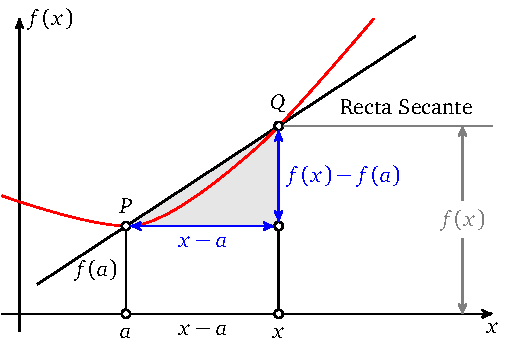
\includegraphics[scale=0.6]{20_home_antalcides_Calculo_pdf_derivada-1.pdf}\caption{Recta secante}
\label{sect}

\end{figure}

Supongamos que queremos hallar la tangente a una curva de ecuación
cartesiana $y=f(x)$ en el punto $(a,f(a))$. La estrategia, usada
primero por Pierre de Fermat y más tarde por Newton, consiste en aproximar
la tangente por rectas secantes cuyas pendientes sí pueden calcularse
directamente. En particular, consideremos la recta que une el punto
$(a,f(a))$ con un punto cercano, $(x,f(x))$, de la gráfica de $f$.
Esta recta se llama una secante (recta que corta a la curva, pero
no es tangente a la curva). La pendiente de esta secante es: 
\[
\frac{f(x)-f(a)}{x-a}
\]
dicho número suele llamarse \emph{cociente incremental de $f$ en
$a$}.

%\begin{floatingfigure}{95cm}%\flushleft 

%\caption{Recta secante}
%\label{sect}
%\end{floatingfigure}

Observa que una secante es una buena aproximación de la tangente,
siempre que el punto $Q(x,f(x))$ esté próximo al punto $P(a,f(a))$.
Estas consideraciones llevan a \emph{definir la tangente a la gráfica
de $f$ en el punto $P(a,f(a))$ como la recta que pasa por dicho
punto y cuya pendiente es igual al límite}: 
\[
\lim_{x\to a}\frac{f(x)-f(a)}{x-a}
\]
supuesto, claro está, que dicho límite exista. 

\subsection{Razón de cambio puntual y velocidad instantánea}

Muchas leyes de la Física, la Química, la Biología o la Economía,
son funciones que relacionan una variable ``dependiente'' $y$ con
otra variable ``independiente'' $x$, lo que suele escribirse en
la forma $y=f(x)$. Si la variable independiente cambia de un valor
inicial $a$ a otro $x$, la variable $y$ lo hace de $f(a)$ a $f(x)$.
La \emph{razón de cambio promedio de $y=f(x)$ con respecto a $x$
en el intervalo $[a,x]$} es: 
\[
\textrm{Razón de cambio promedio\ }=\frac{f(x)-f(a)}{x-a}
\]
Con frecuencia interesa considerar la razón de cambio en intervalos
cada vez más pequeños. Esto lleva a definir lo que podemos llamar
``\emph{razón de cambio puntual de $y=f(x)$ con respecto a $x$
en el punto $a$}'' como: 
\[
\lim_{x\to a}\frac{f(x)-f(a)}{x-a}.
\]
El ejemplo más conocido de esto que decimos es el de un móvil que
se mueve a lo largo de una recta sobre la cual hemos elegido un origen.
Sea $s(t)$ la posición del móvil en el tiempo $t$, es decir, la
distancia con signo del móvil al origen en el tiempo $t$. La razón
de cambio promedio tiene en este caso una interpretación física natural:
\[
\frac{s(a+h)-s(a)}{h}
\]
Es la \emph{velocidad media} del móvil en el intervalo de tiempo comprendido
entre $a$ y $a+h$. Parece intuitivo que, en cada instante, el móvil
se mueve con una determinada \emph{velocidad instantánea}. Pero no
hay manera de medir directamente una velocidad instantánea; un instante
quiere decir una posición en la recta: la velocidad instantánea del
móvil para $t=a$ es la velocidad que tiene cuando está en la posición
$s(a)$. La velocidad instantánea es una abstracción de un característica
física del movimiento, pero no es una magnitud que podamos observar
directamente. La única definición razonable de velocidad instantánea
es como la razón de cambio puntual: 
\[
\lim_{h\to0}\frac{s(a+h)-s(a)}{h}
\]

\noindent \textbf{Notación}.\ En lo que sigue usaremos las letras
$I$, $J$ para representar intervalos no vacíos de números reales.

\begin{defi}{Derivada en un punto}{def}\label{def:derivada} Se dice
que una función \func{f}{I}\ es \textbf{derivable en un punto
$a\in I$}, si existe el límite: 
\[
\lim_{x\to a}\frac{f(x)-f(a)}{x-a}.
\]
Explícitamente, $f$ es derivable en $a$ si hay un número $L\in\R$
verificando que para cada número $\varepsilon>0$ existe algún número
$\delta>0$ tal que para todo $x\in I$ con $x\neq a$ y %
\mbox{%
$\mid x-a\mid<\delta$%
} se tiene que: 
\[
\left|\frac{f(x)-f(a)}{x-a}\ -\ L\right|\leqslant\varepsilon.
\]
Dicho número $L$ se llama \textbf{derivada de $f$ en $a$} y lo
representaremos por $f\tl(a)$ (notación debida a Lagrange). \end{defi}

\begin{defi}{Derivada de una función}{} Dada una función $f:I\rightarrow\R$
derivable en todo punto de $I$, la \textbf{función derivada} de $f$
es la función $f\tl:I\rightarrow\R$ que a cada punto $x\in I$ hace
corresponder la derivada de $f$ en dicho punto. \end{defi}

\begin{ideabox}\label{ob:propiedadlocalderivada} \textbf{i)}\ El
límite $\ {\displaystyle \lim_{x\to a}\frac{f(x)-f(a)}{x-a}}$ se
puede escribir también de la forma $\ {\displaystyle \lim_{h\to0}\frac{f(a+h)-f(a)}{h}.}$

\noindent \textbf{ii)}\ La derivabilidad de $f$ en un punto $a\in I$
es una \emph{propiedad local}, depende solamente del comportamiento
de $f$ en los puntos de $I$ próximos al punto $a$. Concretamente,
si $J$ es cualquier \emph{intervalo abierto} que contiene el punto
$a$, se verifica que $f$ es derivable en $a$ si, y sólo si, la
función restricción $f_{|I\cap J}$ es derivable en $a$ y, por supuesto,
en tal caso ambas funciones tienen la misma derivada en $a$. \end{ideabox}

\noindent \textbf{La notación diferencial de Leibniz.}\ La notación
$\dfrac{\df{f(x)}}{\df{x}}$ para representar la derivada de $f$
en $x$ es debida a Leibniz.

Leibniz interpretaba ese símbolo como un ``cociente diferencial''
pues él lo entendía así: como un cociente de cantidades infinitesimales,
y lo manejaba como un cociente; por ejemplo, se puede multiplicar
o dividir, según convenga, por $\df{x}$ o $\df{f(x)}$. En el capítulo
5 hemos visto los problemas que planteaba el uso de cantidades infinitesimales,
y cómo, finalmente, a partir del último tercio del siglo XIX, fueron
totalmente abandonadas. Por eso, la interpretación de Leibniz de la
derivada, aunque intuitiva, no es la que se sigue en la gran mayoría
de los cursos de cálculo\footnote{Aunque sí en los cursos de Análisis No Estándar basados en los hiperreales
de A. Robinson.}.

A pesar de lo dicho, es frecuente, sobre todo en libros de ingeniería,
usar la notación de Leibniz y manejarla como él lo hacía. Creo que
esto es útil porque la notación de Leibniz tiene una gran fuerza heurística,
y no debe presentar ningún problema, siempre que no acabes creyendo
que una derivada, tal como la hemos definido, es un cociente de infinitésimos.
Y siempre que dicha notación se use como un mero simbolismo y no se
hagan demostraciones apoyadas en su supuesta significación.

Una dificultad de la notación de Leibniz es que no es cómoda para
representar la derivada en un punto concreto. Podemos entender que
$\dfrac{\df{f(x)}}{\df{x}}$ es la función derivada $f\tl(x)$, pero
¿cómo indicamos la derivada en punto concreto $a$? Las notaciones
$\dfrac{\df{f(a)}}{\df{x}}$ y $\dfrac{\df{f(x)}}{\df{x}}(a)$ son
confusas. Lo que suele hacerse es escribir: 
\[
\left.\dfrac{\df{f(x)}}{\df{x}}\right|_{x=a}
\]
que, realmente, es una notación incómoda. Una posible mejora sería
escribir $\dfrac{\df{f}}{\df{x}}(x)$ para representar $f\tl(x)$,
en cuyo caso $\dfrac{\df{f}}{\df{x}}(a)$ indicaría $f\tl(a)$.

La verdad es que la mayoría de los libros de ingeniería que usan estas
notaciones lo hacen sin preocuparse mucho por su significado, y esa
es una causa importante de que muchas veces no se entienda bien lo
que escriben. Las notaciones son importantes y hay que manejarlas
cuidadosamente. Y todavía más, cuando una notación se supone que tiene
un significado casi mágico, y que por su fuerza simbólica ella sola,
por sí misma, proporciona demostraciones. Volveremos a considerar
este asunto más adelante.

\begin{defi}{Recta tangente}{} Supuesto que $f$ es derivable en
$a$, la recta de ecuación cartesiana: 
\[
y=f(a)+f\tl(a)(x-a)
\]
se llama \textbf{recta tangente} a la gráfica de $f$ en el punto
$(a,f(a))$, y también recta tangente a $f$ en $x=a$.

Cuando $f\tl(a)\neq0$, la recta de ecuación: 
\[
y=f(a)-\dfrac{1}{f\tl(a)}(x-a)
\]
es la \textbf{recta normal} a la gráfica de $f$ en el punto $(a,f(a))$,
y también recta normal a $f$ en $x=a$ \end{defi}

\subsubsection{Elementos de una curva relacionados con la derivada}

En la figura~\ref{figcurva} se han representado algunos elementos
de una curva que se expresan por medio de la derivada.

\begin{figure}[H]
\centering 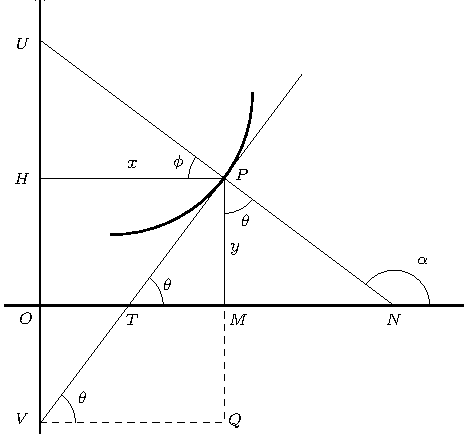
\includegraphics[scale=0.8]{21_home_antalcides_Calculo_pdf_rtan.pdf}\caption{\label{figcurva}{\small{}{Elementos de una curva relacionados con
la derivada}}}
\end{figure}

\begin{itemize}
\item La pendiente de la tangente es $\tg(\theta)=y\tl$. 
\item La pendiente de la normal es $\tg(\alpha)=\tg(\pi/2+\theta)=-1/y\tl$. 
\item El segmento $\overline{TM}$ es la \textbf{subtangente}. Su longitud
viene dada por $\overline{TM}=y\cotg(\theta)=y/y\tl$. 
\item El segmento $\overline{MN}$ es la \textbf{subnormal}. Su longitud
viene dada por $\overline{MN}=y\tg(\theta)=yy\tl$. 
\item Los segmentos interceptados en los ejes $OX$ y $OY$ por la tangente
son 
\[
\begin{cases}
\overline{OT}=\overline{OM}-\overline{TM}=x-y/y\tl\\
\overline{OV}=\overline{PM}-\overline{PQ}=y-x\tg(\theta)=y-xy\tl
\end{cases}
\]
\item Los segmentos interceptados en los ejes $OX$ y $OY$ por la normal
son 
\[
\begin{cases}
\overline{ON}=\overline{OM}+\overline{MN}=x+y\tg(\theta)=x+yy\tl\\
\overline{OU}=\overline{OH}+\overline{HU}=y+x\tg(\phi)=y+x\tg(\pi/2-\theta)=y+x/y\tl
\end{cases}
\]
\end{itemize}

\subsection{Derivadas laterales}

\begin{defi}{Derivadas laterales}{} Se dice que $f$ es \textbf{derivable
por la izquierda en $a$} si existe el límite: 
\[
\lim_{\substack{x\to a\\
x<a
}
}\frac{f(x)-f(a)}{x-a}.
\]
El valor de dicho límite se llama la \textbf{derivada por la izquierda}
de $f$ en $a$.

Análogamente se dice que $f$ es \textbf{derivable por la derecha
en $a,$} si existe el límite: 
\[
\lim_{\substack{x\to a\\
x>a
}
}\frac{f(x)-f(a)}{x-a}.
\]
El valor de dicho límite se llama la \textbf{derivada por la derecha}
de $f$ en $a$. \end{defi}

Teniendo en cuenta la relación que hay entre el límite de una función
en un punto y los límites laterales, es claro que: 
\begin{itemize}
\item[i)] Si $a=\max I$, entonces la derivabilidad de $f$ en $a$ es lo mismo
que la derivabilidad por la izquierda de $f$ en $a$. 
\item[ii)] Si $a=\min I$, entonces la derivabilidad de $f$ en $a$ es lo mismo
que la derivabilidad por la derecha de $f$ en $a$. 
\item[iii)] Si $a$ no es un extremo de $I$, entonces equivalen las afirmaciones: 
\begin{itemize}
\item[a)] $f$ es derivable en $a$. 
\item[b)] Las derivadas por la izquierda y por la derecha de $f$ en $a$ existen
y coinciden. 
\end{itemize}
\end{itemize}

\subsection{Propiedades de las funciones derivables. Reglas de derivación}

El siguiente resultado nos dice que la derivabilidad es una propiedad
más fuerte que la continuidad.

\begin{proposicion}{}{} Toda función derivable en un punto es continua
en dicho punto. \end{proposicion}

\begin{prueba} En efecto, si \func{f}{I}\ es derivable en $a$,
de la igualdad: 
\[
f(x)=f(a)+(x-a)\frac{f(x)-f(a)}{x-a}\quad(x\en I,\ x\neq a)
\]
se sigue que $\dis\lim_{x\to a}f(x)=f(a)$, es decir, $f$ es continua
en $a$.\end{prueba}

\begin{teo}{Reglas de derivación}{}\ Sean \func{f,g}{I}\ dos
funciones. Se verifican las siguientes afirmaciones: 
\begin{itemize}
\item[i)] La funciones suma, $f+g$, y producto, $fg$, son derivables en todo
punto $a\en I$ en el que $f$ y $g$ sean derivables, y las derivadas
respectivas vienen dadas por:

\[
(f+g)^{\prime}(a)=f\tl(a)+g\tl(a);\quad(fg)^{\prime}(a)=f\tl(a)g(a)+f(a)g\tl(a)
\]

\item[ii)] Si $g(x)\neq0$ para todo $x\in I$, la función cociente $f/g$ es
derivable en todo punto $a\en I$ en el que $f$ y $g$ sean derivables,
en cuyo caso se verifica que: 
\[
\left(\frac{f}{g}\right)^{\prime}(a)=\frac{f\tl(a)g(a)-f(a)g\tl(a)}{(g(a))^{2}}
\]
\end{itemize}
\end{teo} 

\begin{prueba} Las reglas de derivación se prueban muy fácilmente
haciendo uso de las propiedades algebraicas de los límites y la definición
de derivada. Es suficiente que tengas en cuenta las siguientes igualdades:
\begin{eqnarray*}
\dfrac{(f+g)(x)-(f+g)(a)}{x-a} & = & \dfrac{f(x)-f(a)}{x-a}+\dfrac{g(x)-g(a)}{x-a}\\
\dfrac{(fg)(x)-(fg)(a)}{x-a} & = & \dfrac{f(x)-f(a)}{x-a}g(x)+f(a)\dfrac{g(x)-g(a)}{x-a}\\
\dfrac{\frac{1}{g}(x)-\frac{1}{g}(a)}{x-a} & = & -\dfrac{g(x)-g(a)}{x-a}\dfrac{1}{g(x)g(a)}
\end{eqnarray*}
De la primera y segunda igualdades se deduce, tomando límites para
$x\to a$ , las reglas para la derivada de una suma y de un producto.
Igualmente, de la tercera igualdad, se deduce la derivada de $\frac{1}{g}$,
de donde, se obtiene la derivada de $\frac{f}{g}=f\frac{1}{g}$ haciendo
uso de la regla para derivar un producto.\end{prueba}

Como las funciones constantes tienen derivada nula en todo punto y
la función identidad, $f(x)=x$, tiene derivada igual a 1 en todo
punto, aplicando las reglas de derivación anteriores se obtiene el
siguiente corolario.

\begin{coro}{}{} Las funciones polinómicas son derivables en todo
punto y las funciones racionales son derivables en todo punto de su
conjunto natural de definición. Además la derivada de la función polinómica
\mbox{%
$\ f(x)=a_{0}+a_{1}x+a_{2}x^{2}+\cdots+a_{n}x^{n}$\ %
} en cada punto $x\in\R$ viene dada por: 
\[
f\tl(x)=a_{1}+2a_{2}x+3a_{3}x^{2}+\cdots+na_{n}x^{n-1}
\]
\end{coro}

\begin{teo}{Derivación de una función compuesta o regla de la cadena}{}{}

Sean \func{f}{I}\ y \func{g}{J}\ con $f(I)\subset J$,
y sea \func{h=g\!\circ \!f}{I}\ la función compuesta. Supongamos
que $f$ es derivable en $a\en I$ y que $g$ es derivable en $f(a)$.
Entonces $h$ es derivable en $a$ y $h\tl(a)=g\tl(f(a))f\tl(a)$.

\noindent En particular, si $g$ es derivable en $J$, la función
compuesta $h=g\!\circ\!f$ es derivable en todo punto de $I$ donde
$f$ sea derivable. \end{teo}

\noindent \begin{prueba} Pongamos $b=f(a)$. Tenemos que probar que
$\dis{\lim_{x\to a}\frac{h(x)-h(a)}{x-a}=g\tl(b)f\tl(a)}$. Por hipótesis
se cumple que :
\[
\lim_{y\to b}\frac{g(y)-g(b)}{y-b}\lim_{x\to a}\frac{f(x)-f(a)}{x-a}=g\tl(b)f\tl(a)
\]
La idea de la demostración es hacer en esta igualdad la sustitución
$y=f(x)$. Como no está garantizado por las hipótesis hechas que para
$x\neq a$ se tenga %
\mbox{%
$f(x)\neq b$,%
} no está justificado hacer directamente la sustitución indicada (dividir
por cero está prohibido). Podemos evitar esta dificultad como sigue.
Definamos la función \func{\ff}{J}\ por: 
\[
\ff(y)=\frac{g(y)-g(b)}{y-b}\ \ (y\neq b),\ \ff(b)=g\tl(b)
\]
Con ello la función \ff\ es continua en $b$. Es inmediato ahora
comprobar que para todo $x\en I$ con $x\neq a$ se verifica que:
\begin{equation}
\frac{h(x)-h(a)}{x-a}=\ff(f(x))\frac{f(x)-f(a)}{x-a}.\label{equality}
\end{equation}
Ahora, como $f$ es continua en $a$ (porque es derivable en $a$)
y \ff\ es continua en $b=f(a)$, se sigue que $\ff\circ f$ es continua
en $a$, por lo que: 
\[
\lim_{x\to a}\ff(f(x))=\ff(f(a))=\ff(b)=g\tl(b).
\]
La igualdad (\ref{equality}) nos dice ahora que:
\[
\lim_{x\to a}\frac{h(x)-h(a)}{x-a}=g\tl(b)f\tl(a)
\]
como queríamos probar.\end{prueba}

\noindent \textbf{Regla de la cadena al estilo Leibniz.} Una demostración
de la regla de la cadena al ``estilo Leibniz'' podría ser como sigue.
Por una parte, tenemos que $y$ es función de $x$ a través de $g$,
es decir, $y=g(x)$. También tenemos que $x$ es función de $t$ a
través de $f$, $x=f(t)$. Entonces la variación de $y$ respecto
a $t$ se hace por intermedio de $x$: 
\begin{equation}
\frac{\df{y}}{\df{t}}=\frac{\df{y}}{\df{x}}\frac{\df{x}}{\df{t}}\label{cadenaleibniz}
\end{equation}
Hemos acabado. Todo lo que hemos hecho ha sido multiplicar y dividir
por $\df{x}$.

No sé lo que pensará tú de esto, pero a mí me parecería una broma
que alguien pretendiera que lo que hemos hecho es una demostración.
Primero: ¿qué es $\df{x}$? Porque si es un símbolo, no tiene sentido
multiplicar y dividir por él (salvo que a esta operación se le hubiera
asignado previamente un significado preciso) y si es un número ¿cómo
está definido? ¿qué relación tiene ese número con la derivada? Preguntas
sin respuesta. A esto me refería al decir que una notación, por sí
sola, no sirve para demostrar nada.

Además, el simbolismo empleado en la igualdad (\ref{cadenaleibniz})
no indica dónde se evalúa cada una de las derivadas, y eso es fundamental
para entender la regla de la cadena. Fíjate que la regla de la cadena
nos dice que la derivada de una función compuesta de dos funciones
derivables, $h(x)=(g\circ f)(x)$, viene dada por 
\begin{equation}
h\tl(x)=g\tl(f(x))f\tl(x)=(g\tl\circ f)(x)f\tl(x)\label{cadenalagrange}
\end{equation}
que es un producto de dos funciones, $g\tl(f(x))$ y $f\tl(x)$, pero
la primera de ellas $g\tl(f(x))=(g\tl\circ f)(x)$ es una \emph{función
compuesta}. Por eso si queremos volver a derivar en la igualdad (\ref{cadenalagrange}),
debemos aplicar la regla para derivar un producto y, para derivar
el primer factor, debemos aplicar la regla de la cadena. Es por eso
que, en la regla de la cadena, es fundamental indicar los puntos donde
se evalúan las derivadas.

La notación en la igualdad (\ref{cadenaleibniz}) es mala porque no
indica dónde se evalúa cada una de las derivadas. Pero también es
mala por las razones siguientes.

$\bullet\quad$Una misma letra representa dos funciones distintas.
En (\ref{cadenaleibniz}) la letra $y$ aparece a la izquierda y a
la derecha. A la izquierda representa la función compuesta $y=g(f(t))$,
a la derecha representa la función $y=g(x)$.

\indent$\bullet\quad$Una misma letra representa una función y una
variable. La letra $x$ en la parte derecha representa la variable
en $y=g(x)$, y también representa la función $x=f(t)$.

Demasiado confuso ¿verdad? A pesar de lo dicho, la igualdad (\ref{cadenaleibniz})
aparece en muchos textos de matemáticas para ingenieros y en textos
de física, sin ningún comentario, sin explicar lo que significa y
pretendiendo que constituye por sí misma una demostración. Lo peor
de todo, es que si te la enseñan así puedes creer que la entiendes,
y entonces una de dos: o la entiendes de verdad, como acabo de explicarlo,
o te engañas y realmente no sabes lo que crees saber. Lamentablemente,
de estas dos posibilidades la más frecuente es la segunda.

Y…sin embargo, la igualdad (\ref{cadenaleibniz}) es muy simple y
fácil de recordar, y permite conjeturar la regla de la cadena sin
necesidad de demostrarla (por eso decimos que la notación de Leibniz
tiene un gran valor heurístico). Mi consejo es el siguiente: puedes
usar la notación de Leibniz siempre que te ayude en lo cálculos, pero
no debes dejarte llevar por la notación sino que debes entender lo
que estás haciendo en cada momento.

\begin{ejemplo} Sabiendo que $y=\sen x$ y $x=\cos t$, se pide calcular
la derivada de $y$ con respecto a $t$.

Lo que nos piden es calcular la derivada de la función compuesta $h(t)=\sen(\cos t)$.
Aquí $g(x)=\sen x$, $f(t)=\cos t$. Tenemos que 
\[
h\tl(t)=g\tl(f(t))f\tl(t)=-\cos(\cos t)\sen t
\]
Al estilo Leibniz: 
\[
\frac{\df{y}}{\df{t}}=\frac{\df{y}}{\df{x}}\frac{\df{x}}{\df{t}}=\cos x(-\sen t)=-\cos x\sen t
\]
Pero esta igualdad debe ser función de $t$ por lo que hay que sustituir
$x=\cos t$ y se vuelve a obtener el resultado anterior. \end{ejemplo}

\subsection{Derivación implícita}

\subsection{Derivada de la la función inversa}

\subsection{Derivabilidad de las funciones Transcendentales}

\subsubsection{Derivabilidad de la exponencial y del logaritmo. Criterio de equivalencia
logarítmica}

Aceptaremos que las funciones logaritmo, exponencial, trigonométricas
y sus inversas, son derivables, pues ahora no sería fácil probarlo.
Más adelante dispondremos de herramientas para hacerlo con comodidad.

La función exponencial $x\mapsto\exp(x)=\e^{x}$, $(x\in\R)$, y la
función logaritmo natural %
\mbox{%
$x\mapsto\log x$%
}, $(x\in\R^{+})$, son derivables en todo punto de sus respectivos
intervalos de definición, siendo: 
\[
(\exp)^{\prime}(x)=\exp x\ \ensuremath{\forall x\in\R),\ \ \ \ (\log)^{\prime}(x)=\frac{1}{x}\ \ensuremath{\forall x\in\R^{+})}}
\]
En particular, se verifica que: 
\[
\dis{\lim_{x\to1}\frac{\log x}{x-1}=1;\quad\lim_{x\to0}\frac{\e^{x}-1}{x}=1;\quad\lim_{x\to0}\frac{\log(1+x)}{x}=1;\quad\lim_{x\to0}(1+x)^{1/x}=\e}
\]
Pues los primeros tres límites son derivadas y el cuarto se reduce
fácilmente al tercero. Deducimos también un importante resultado que
permite resolver en muchos casos las indeterminaciones ``$1^{\infty}$''
y ``$0\infty$''.

\begin{teo}{Criterio de equivalencia logarítmica}{}\label{zapato}
Sea $a\en I$, $f$ y $g$ funciones definidas en %
\mbox{%
$I\setminus\{a\}$.%
} Supongamos que $f(x)>0$ para $x\en I\setminus\{a\}$, y que $\dis\lim_{x\to a}f(x)=1$.
Entonces se tiene que: 
\begin{itemize}
\item[i)] $\dis\lim_{x\to a}f(x)^{g(x)}=\e^{L}\ $ si, y sólo si, $\dis\lim_{x\to a}g(x)(f(x)-1)=L$. 
\item[ii)] $\dis\lim_{x\to a}f(x)^{g(x)}=+\infinity\ $ si, y sólo si, $\dis\lim_{x\to a}g(x)(f(x)-1)=+\infinity$. 
\item[iii)] $\dis\lim_{x\to a}f(x)^{g(x)}=0\ $ si, y sólo si, $\dis\lim_{x\to a}g(x)(f(x)-1)=-\infinity$. 
\end{itemize}
\end{teo} \dem Sea \func{\ff}{\Rp}\ la función dada por:
\[
\ff(x)=\frac{\log x}{x-1},\ (x\neq1),\ \ff(1)=1.
\]
Nótese que \ff\ es una función continua. Pongamos: 
\[
f(x)^{g(x)}=\exp\big(g(x)\log(f(x))\big)=\exp\big(g(x)(f(x)-1)\ff(f(x))\big)
\]
Puesto que $\dis\lim_{x\to a}\ff(f(x))=1$ se sigue que: 
\[
\lim_{x\to a}g(x)(f(x)-1)\ff(f(x))=L\en\R\cup\{+\infinity\}\cup\{-\infinity\}
\]
si, y sólo si 
\[
\lim_{x\to a}g(x)(f(x)-1))=L\en\R\cup\{+\infinity\}\cup\{-\infinity\}
\]
lo que prueba las afirmaciones hechas.\fin

Las afirmaciones que se hacen en la siguiente proposición son consecuencia
fácil de la regla de la cadena.

\begin{proposicion}{}{} Sean $f,g:I\rightarrow\R$, $a\en I$ y $g(x)>0$
para todo $x\in I$. Se verifica entonces que:\\
i) $f$ es derivable en $a$ si, y sólo si, la función $h(x)=\exp(f(x))$
es derivable en $a$ en cuyo caso $\ h^{\prime}(a)=f\tl(a)\exp(f(a))$.\\
ii) $g$ es derivable en $a$ si, y sólo si, la función $\varphi(x)=\log(g(x))$
es derivable en $a$ en cuyo caso ${\ {\displaystyle \varphi\tl(a)=\frac{g\tl(a)}{g(a)}.}}$\\
iii) Si $f$ y $g$ son derivables en $a$ la función $\psi(x)=g(x)^{f(x)}$
también es derivable en $a$ y 
\[
\psi\tl(a)=\psi(a)\left(\log(g(a))f\tl(a)+f(a)\frac{g\tl(a)}{g(a)}\right)
\]
\end{proposicion}

Te recuerdo que una forma cómoda para trabajar con funciones de la
forma $\psi(x)=g(x)^{f(x)}$ es escribirlas como exponenciales $\psi(x)=\exp\big(f(x)\log(g(x))\big)$.\vspace*{-3mm}


\subsubsection{Derivación logarítmica}

\subsubsection{Derivabilidad de las funciones trigonométricas}

Las funciones seno y coseno son derivables en todo punto verificándose
que: 
\[
\sen\tlo(x)=\cos x\quad\cos\tlo(x)=-\sen x.
\]
En particular, se verifica que: 
\[
\lim_{x\to0}\dfrac{\sen x}{x}=1,\quad\lim_{x\to0}\dfrac{\cos x-1}{x}=0.
\]
Las derivadas de las demás funciones trigonométricas se deducen con
facilidad a partir de las derivadas del seno y del coseno. \vspace*{-3mm}


\subsubsection{Derivabilidad de las funciones hiperbólicas}

Las derivadas de las funciones hiperbólicas y de sus inversas se deducen
con facilidad de las derivadas del logaritmo y de la exponencial.
Se comprueba sin dificultad que 
\[
\senh\tlo(x)=\cosh x,\quad\cosh\tlo(x)=\senh x
\]
Las derivadas de las funciones hiperbólicas inversas son muy útiles
para calcular primitivas de funciones en las que intervienen raíces
cuadradas de trinomios de segundo grado. 
\begin{center}
\begin{tabular}{|c|c|}
\hline 
% after \\: \hline or \cline{col1-col2} \cline{col3-col4} ...
\raisebox{1em}{$\rule{0mm}{9mm}\dis\argsenh(x)=\log\left(x+\sqrt{x^{2}+1}\right)$}  &
\raisebox{1em}{$\rule{0mm}{9mm}\dis\argsenh\tlo(x)=\frac{1}{\sqrt{x^{2}+1}}$} \tabularnewline
\hline 
\raisebox{1em}{$\rule{0mm}{9mm}\dis\argcosh(x)=\log\left(x+\sqrt{x^{2}-1}\right)\quad x>1$}  &
\raisebox{1em}{$\rule{0mm}{9mm}\dis\argcosh\tlo(x)=\frac{1}{\sqrt{x^{2}-1}}$} \tabularnewline
\hline 
\raisebox{1em}{$\rule{0mm}{9mm}\dis\argcosech(x)=\argsenh\left(\dfrac{1}{x}\right)\quad x\neq0$}  &
\raisebox{1em}{$\rule{0mm}{9mm}\dis\argcosech\tlo(x)=\frac{-1}{\abs{x}\sqrt{x^{2}+1}}$} \tabularnewline
\hline 
\raisebox{1em}{$\rule{0mm}{9mm}\dis\argsech(x)=\argcosh\left(\dfrac{1}{x}\right)\quad0<x<1$}  &
\raisebox{1em}{$\rule{0mm}{9mm}\dis\argsech\tlo(x)=\frac{-1}{x\sqrt{1-x^{2}}}$} \tabularnewline
\hline 
\end{tabular}
\par\end{center}

\begin{ejercicios propuestos} 

\selectlanguage{english}%
\item[]\emph{Empezaremos con algunas de las aplicaciones más sencillas 
y atractivas del cálculo diferencial. En esquema, se trata de lo siguiente: 
calcular la tasa de variación} de una magnitud cuando se conoce la 
tasa de variación de otra magnitud relacionada con ella. En este tipo 
de ejercicios la tasa de variación se interpreta como una derivada 
y, en la mayorí­a de los casos, basta usar la regla de la cadena para 
obtener lo que se pide. Hay que elegir las unidades de acuerdo con 
los datos del problema; por ejemplo, si un volumen se mide en litros 
tendremos que medir longitudes con decí­metros.

\selectlanguage{spanish}%
%\setcounter{propuesto}{172}

\propuesto ¿Con qué rapidez baja el nivel del agua contenida en un
depósito cilíndrico si estamos vaciándolo a razón de 3000 litros por
minuto?

\propuesto Se está llenando un globo de forma esférica con gas a
razón de 50cm$^{3}$/s. Calcula la velocidad a la que está aumentando
el radio, $r$, del globo cuando su valor es $r=5$.

\propuesto Un punto $P$ se mueve sobre la parte de la parábola $x=y^{2}$
situada en el primer cuadrante de forma que su coordenada $x$ está
aumentando a razón de 5cm/sg. Calcula la velocidad a la que el punto
$P$ se aleja del origen cuando $x=9$.

\propuesto Se está llenando un depósito cónico apoyado en su vértice
a razón de 9 litros por segundo. Sabiendo que la altura del depósito
es de 10 metros y el radio de la tapadera de 5 metros, ¿con qué rapidez
se eleva el nivel del agua cuando ha alcanzado una profundidad de
6 metros?

\propuesto El volumen de un cubo está aumentando a razón de 70cm$^{3}$
por minuto. ¿Con qué rapidez está aumentando el área cuando la longitud
del lado es de 12cm?

\propuesto Un barco $A$ se desplaza hacia el oeste con una velocidad
de 20 millas por hora y otro barco $B$ avanza hacia el norte a 15
millas por hora. Ambos se dirigen hacia un punto $O$ del océano en
el cual sus rutas se cruzan. Sabiendo que las distancias iniciales
de los barcos $A$ y $B$ al punto $O$ son, respectivamente, de 15
y de 60 millas, se pregunta: ¿A qué velocidad se acercan (o se alejan)
los barcos entre sí cuando ha transcurrido una hora? ¿Y cuando han
transcurrido 2 horas? ¿En qué momento están más próximos uno de otro?

\propuesto Una bola esférica de hielo se está derritiendo de forma
uniforme en toda la superficie, a razón de 50cm$^{3}$ por minuto.
¿Con qué velocidad está disminuyendo el radio de la bola cuando este
mide 15cm?

\propuesto Un hombre se aleja de una farola a razón de 1,5m/sg. Sabiendo
que la altura del hombre es de 1,8 metros y la de la farola de 15
metros, calcula la velocidad a la que está aumentando la sombra del
hombre proyectada por la luz.

\propuesto Un faro, cuya linterna gira a 8 revoluciones por minuto,
se encuentra situado a 3 kilómetros de una costa rectilínea. Calcula
la velocidad con que el rayo de luz recorre la orilla cuando el ángulo
de incidencia del rayo de luz con la línea de la costa es de 45 grados.

\bigskip{}

\emph{Los siguientes ejercicios son de cálculo de derivadas y de tangentes
y normales a distintas curvas. Cuando en un ejercicio intervienen
parámetros, debes expresar las soluciones de la forma más sencilla
posible.}

\bigskip{}

\propuesto Calcula $(f\circ g)^{\prime}(x)$ en el valor indicado
de $x$ en los siguientes casos: 
\begin{enumerate}
\item $\dis{f(x)=\frac{2x}{x^{2}+1},\quad g(x)=10x^{2}+x+1,\quad x=0}$ 
\item $\dis{f(x)=\left(\frac{x-1}{x+1}\right)^{2},\quad g(x)=\frac{1}{x^{2}}-1,\quad x=-1}$ 
\end{enumerate}
\propuesto Calcula en cada caso el valor de $a$ y $b$ en función
de $c$, para que exista la derivada en el punto $c$ de cada una
de las siguientes funciones: 
\[
f(x)=\left\{ \begin{array}{ll}
x^{2}, & x\le c\\
ax+b, & x>c
\end{array}\right.\ \ f(x)=\left\{ \begin{array}{ll}
\dfrac{1}{\abs{x}}, & \abs{x}>c\\
a+bx^{2}, & \abs{x}\le c
\end{array}\right.\ \ f(x)=\left\{ \begin{array}{ll}
\cos x, & x\le c\\
ax+b, & x>c
\end{array}\right.
\]
\propuesto Supongamos que $f$ es derivable en $a$, $g$ es continua
en $a$ y $f(a)=0$. Prueba que $fg$ es derivable en $a$.

\propuesto ¿Es cierta la igualdad ${\displaystyle f\tl(a)=\lim_{t\to a}\dfrac{f(a+t)-f(a-t)}{2t}}$?
Justifica tu respuesta.

\propuesto Supongamos que las funciones $f$ y $g$ y sus derivadas
tienen los siguientes valores en $x=2$ y $x=3$.
\begin{center}
\begin{tabular}{|c|c|c||c|c|}
\hline 
$x$ &
$f\left(x\right)$ &
$g\left(x\right)$ &
$f\tl\left(x\right)$ &
$g\tl\left(x\right)$\tabularnewline
\hline 
\hline 
2 &
8 &
2 &
$\frac{1}{3}$ &
-3\tabularnewline
\hline 
3 &
3 &
-4 &
$2\pi$ &
5\tabularnewline
\hline 
\end{tabular}
\par\end{center}

Calcular las derivadas de las siguientes funciones en los valores
dados de $x$:

\begin{tabular}{ll}
a)\ $f(x)g(x),\quad x=3\qquad\quad$  &
b)$\ f(x)/g(x),\quad x=3$\tabularnewline
c)\ $f(g(x)),\quad x=2$  &
d)\ $\sqrt{\rule{0mm}{3.5mm}(f(x))^{2}+(g(x))^{2}},\quad x=2$ \tabularnewline
\end{tabular}

\propuesto Supongamos que las funciones $f$ y $g$ y sus derivadas
tienen los valores que se indican en la tabla.
\begin{center}
\begin{tabular}{|c|c|c|c|c|}
\hline 
$x$ &
$f\left(x\right)$ &
$g\left(x\right)$ &
$f\tl\left(x\right)$ &
$g\tl\left(x\right)$\tabularnewline
\hline 
\hline 
0 &
1 &
5 &
2 &
-5\tabularnewline
\hline 
1 &
3 &
-2 &
0 &
1\tabularnewline
\hline 
3 &
2 &
4 &
1 &
-6\tabularnewline
\hline 
\end{tabular}
\par\end{center}

Calcula una tabla análoga para las funciones $f\circ g$ y $g\circ f$.

\propuesto Calcula directamente, aplicando la definición, la derivada
de $f(x)=x^{3}$ en un punto genérico $a$.

\propuesto Calcula directamente, aplicando la definición, la derivada
de $f(x)=\sqrt{x+7}$ en el punto $a=-1$.

\propuesto Supongamos que $f$ es una función que verifica una desigualdad
del tipo $\abs{f(x)}\le\abs{x}^{r}$ en algún intervalo abierto que
contiene a cero, donde $r>1$. Prueba que $f$ es derivable en $0$.

\propuesto Sea $f$ una función tal que $f(x+h)=f(x)+3xh+h^{2}-2h$
para todos $x,h\en\R$. Calcula $f\tl(0)$ y $f\tl(2)$.

\propuesto Calcula la derivada en todo punto de la función definida
por 
\[
f(x)=\left\{ \begin{array}{ll}
x^{2}\sen\dfrac{1}{x}, & x\neq0\\
0, & x=0
\end{array}\right.
\]
\propuesto Desarrolla $(1+x)^{n}$ por el binomio de Newton y deriva
la igualdad resultante para probar las igualdades siguientes: 
\[
\sum_{k=1}^{n}k\binom{n}{k}=n2^{n-1},\qquad\sum_{k=2}^{n}k(k-1)\binom{n}{k}=n(n-1)2^{n-2}
\]
\propuesto Calcula los puntos en que la cúbica de ecuación $y=ax^{3}+bx^{2}+cx+d$,
donde $a,b,c,d$ son constantes reales, tiene tangente horizontal.
Debes estudiar los distintos casos posibles.

\propuesto Calcula un punto $c$ por la condición de que la tangente
a la parábola $f(x)=x^{2}+\alpha x+\beta$ en el punto $(c,f(c))$,
sea paralela a la cuerda que une dos puntos dados $A=(a,f(a))$ y
$B=(b,f(b))$.

\propuesto Calcula las ecuaciones de las rectas tangente y normal
a una parábola $f(x)=ax^{2}+bx+c$ en un punto genérico $(u,v)$ de
la misma.

\propuesto Calcula las ecuaciones de las rectas tangente y normal
a una hipérbola de ecuación cartesiana $x^{2}-y^{2}=1$, en un punto
genérico $(u,v)$ de la misma.

\propuesto Calcula las ecuaciones de las rectas tangente y normal
a una elipse de ecuación 
\[
\frac{x^{2}}{a^{2}}+\frac{y^{2}}{b^{2}}=1
\]
en un punto $(u,v)$ de la misma. \end{ejercicios propuestos}

\begin{ejercicios resueltos} \resuelto ¿Con qué rapidez baja el
nivel del agua contenida en un depósito cilíndrico si estamos vaciándolo
a razón de 3000 litros por minuto?

\sol Sea $r$ el radio del cilindro y $h$ la altura medidos en decímetros.
Sea $V(t)$ el volumen de agua, medido en litros (dcm$^{3}$), que
hay en el cilindro en el tiempo $t$ medido en minutos. La información
que nos dan es una tasa de variación 
\[
V(t+1)-V(t)=-3000\quad\textrm{litros por minuto}
\]
En este tipo de ejercicios la tasa de variación se interpreta como
una derivada: $V\tl(t)=-3000$. Fíjate que $V(t+t_{0})-V(t_{0})\approxeq V\tl(t_{0})t$,
por lo que la interpretación es razonable. El signo negativo de la
derivada es obligado ya que el volumen disminuye con el tiempo. Como
el radio es constante pero la altura del agua depende del tiempo,
tenemos 
\[
V(t)=\pi r^{2}h(t)
\]
y deducimos 
\[
V\tl(t)=-3000=\pi r^{2}h\tl(t)
\]
Por tanto 
\[
h\tl(t)=-\dfrac{3000}{\pi\,r^{2}}\quad\textrm{decímetros por minuto}
\]
Si expresamos las medidas en metros, entonces $\,h\tl(t)=-\dfrac{3}{\pi r^{2}}$
metros por minuto.

Observa que lo que realmente hemos calculado es: 
\[
V(t+1)-V(t)=\pi r^{2}(h(t+1)-h(t))\quad\longrightarrow\quad h(t+1)-h(t)=\frac{V(t+1)-V(t)}{\pi r^{2}}=-\dfrac{3000}{\pi\,r^{2}}
\]
que es la tasa de variación de la altura en un intervalo de 1 minuto.
Pero, como ya te he dicho, en estos ejercicios se identifica la tasa
de variación con una derivada, lo cual es, claro está, una aproximación.\hecho

\resuelto Un punto $P$ se mueve sobre la parte de la parábola $\,x=y^{2}$
situada en el primer cuadrante de forma que su coordenada $x$ está
aumentando a razón de 5cm/sg. Calcular la velocidad a la que el punto
$P$ se aleja del origen cuando $x=9$.

\sol Sean $(x(t),y(t))$ las coordenadas, medidas en centímetros,
del punto $P$ en el instante $t$ medido en segundos. Nos dicen que
$y(t)\geqslant0$ y que $x(t)=y(t)^{2}$. La distancia del punto $P$
al origen viene dada por $f(t)=\sqrt{x(t)^{2}+y(t)^{2}}$, por lo
que 
\[
f\tl(t)=\frac{x(t)x\tl(t)+y(t)y\tl(t)}{\sqrt{x(t)^{2}+y(t)^{2}}}
\]
Lo que nos piden es $f\tl(t_{0})$ sabiendo que $x(t_{0})=9$. En
tal caso ha de ser $y(t_{0})=3$. También conocemos $x\tl(t)=5$ (cm/sg).
Con ello es fácil deducir el valor de $y\tl(t_{0})=\dfrac{x\tl(t_{0})}{2y(t_{0})}=\dfrac{5}{6}$.
Finalmente, 
\[
f\tl(t_{0})=\frac{x(t_{0})x\tl(t_{0})+y(t_{0})y\tl(t_{0})}{\sqrt{x(t_{0})^{2}+y(t_{0})^{2}}}=\frac{45+3(5/6)}{81+9}=\frac{95}{6\sqrt{10}}\ textrm{cm/sg}
\]
\hecho

\resuelto Se está llenando un depósito cónico apoyado en su vértice
a razón de 9 litros por segundo. Sabiendo que la altura del depósito
es de 10 metros y el radio de la tapadera de 5 metros, ¿con qué rapidez
se eleva el nivel del agua cuando ha alcanzado una profundidad de
6 metros?

\sol Expresaremos todas las medidas en metros. Si $V(t)$ es el volumen
de agua que hay en el depósito en el tiempo $t$ medido en segundos,
nos dicen que $V\tl(t)=\dfrac{9}{10^{3}}$ m$^{3}$/sg.
\begin{figure}[ht]
\centering{}%
\begin{minipage}[c]{0.45\textwidth}%
\vspace{0pt}
 \centering 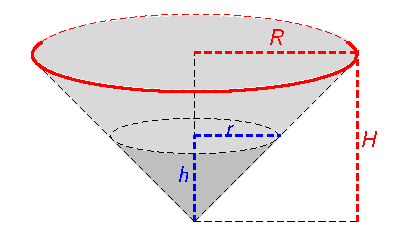
\includegraphics[scale=0.8]{22_home_antalcides_Calculo_pdf_resuelto1.pdf}
\captionsetup{,singlelinecheck=off,margin=1cm} \caption{Depósito cónico}
%
\end{minipage}%
\begin{minipage}[c]{0.55\textwidth}%
 \vspace{-4pt}
 Sabemos que $V(t)=\dfrac{1}{3}\pi\,r(t)^{2}h(t)$ donde $h(t)$ es
la altura, medida desde el vértice, alcanzada por el agua en el tiempo
$t$ y $r(t)$ es el radio de la sección transversal del cono a la
distancia $h(t)$ desde el vértice. Por semejanza de triángulos deducimos
que $\,\dfrac{r}{R}=\dfrac{h}{H}\,$, de donde, $r=r(t)=\dfrac{R}{H}h(t)=\dfrac{1}{2}h(t)$.
Luego $V(t)=\dfrac{1}{12}\pi\,h(t)^{3}$, y 
\[
V\tl(t)=\dfrac{9}{10^{3}}=\dfrac{\pi}{4}h(t)^{2}h\tl(t).
\]
%
\end{minipage}
\end{figure}
Luego, cuando $h(t_{0})=6$, deducimos que $\dfrac{9}{10^{3}}=\dfrac{\pi}{4}36h\tl(t_{0})$,
esto es, $h\tl(t_{0})=\dfrac{1}{10^{3}\pi}\ \textrm{m/sg}\ \approxeq1,146\ \textrm{m/h}$.\hecho

\resuelto El volumen de un cubo está aumentando a razón de 70\,cm$^{3}$
por minuto. ¿Con qué rapidez está aumentando el área cuando la longitud
del lado es de 12\,cm?

\sol Sea $V(t)$ el volumen del cubo, medido en centímetros cúbicos,
en el tiempo $t$, medido en minutos. Si $L(t)$ es la longitud en
centímetros del lado en el tiempo $t$, tenemos que $V(t)=L(t)^{3}$,
de donde, $L\tl(t)=\dfrac{V\tl(t)}{3L(t)^{2}}$. Como nos dicen que
$V\tl(t)=70$ cm/min, deducimos que cuando $L(t_{0})=12$, $L\tl(t_{0})=\dfrac{70}{3(12)^{2}}$.
El área del cubo viene dada por $S(t)=6L(t)^{2}$, deducimos que $\,S\tl(t_{0})=12L(t_{0})L\tl(t_{0})=\dfrac{70}{3}$
cm$^{2}$/min.\hecho

\resuelto Un barco $A$ se desplaza hacia el oeste con una velocidad
de 20 millas por hora y otro barco $B$ avanza hacia el norte a 15
millas por hora. Ambos se dirigen hacia un punto $O$ del océano en
el cual sus rutas se cruzan. Sabiendo que las distancias iniciales
de los barcos $A$ y $B$ al punto $O$ son, respectivamente, de 15
y de 60 millas, se pregunta: ¿A qué velocidad se acercan (o se alejan)
los barcos entre sí cuando ha transcurrido una hora? Y cuando han
transcurrido 2 horas? ?`En qué momento están más próximos uno de otro?

\sol Tomamos el punto $O$ como origen de coordenadas, tal como se
indica en la figura. Llamemos $x(t)$ a la distancia, medida en millas,
que separa el barco $A$ de $O$. Nos dicen que $x(0)=15$ y $x\tl(t)=-20$
millas por hora. Observa que como la función $x(t)$ es decreciente
su derivada debe ser negativa. Análogamente, sea $y(t)$ la distancia
que separa al barco $B$ de $O$.

\begin{figure}[ht]
\centering{}%
\begin{minipage}[c]{0.4\textwidth}%
\begin{center}
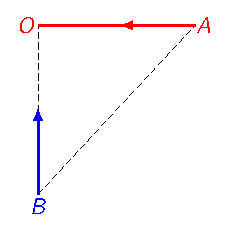
\includegraphics{23_home_antalcides_Calculo_pdf_resuelto2.pdf}
\par\end{center}
\captionsetup{,singlelinecheck=off,margin=1cm} \caption{Cruce de barcos}
%
\end{minipage}%
\begin{minipage}[c]{0.55\textwidth}%
 \vspace{-4pt}
 Nos dicen que $y(0)=60$ y $y\tl(t)=-15$ millas por hora. La distancia
entre los dos barcos viene dada por $\,f(t)=\sqrt{x(t)^{2}+y(t)^{2}}$.
Tenemos 
\[
f\tl(t)=\frac{x(t)x\tl(t)+y(t)y\tl(t)}{\sqrt{x(t)^{2}+y(t)^{2}}}
\]
Cuando ha pasado una hora $x(1)=15-20=-5$, $y(1)=60-15=45$. Deducimos
que 
\[
f\tl(1)=\frac{(-5)(-20)+45(-15)}{\sqrt{(-5)^{2}+(45)^{2}}}=-\frac{115}{\sqrt{82}}\ textrm{millas/h}
\]
Donde el sigo negativo indica que se están acercando (la distancia
entre ellos está disminuyendo). %
\end{minipage}
\end{figure}

\vspace*{10mm}

Cuando han pasado dos horas $x(2)=15-40=-25$, $y(2)=60-30=30$. Deducimos
que 
\[
f\tl(2)=\frac{(-25)(-20)+30(-15)}{\sqrt{(-25)^{2}+(30)^{2}}}=\frac{10}{\sqrt{61}}\ textrm{millas/h}
\]
Donde el sigo positivo indica que se están alejando (la distancia
entre ellos está aumentando).

La distancia entre los dos barcos es mínima cuando la derivada es
nula (fíjate que la derivada pasa de negativa a positiva). La condición
$\,f\tl(t_{0})=0$ equivale a la igualdad $-20\,x(t_{0})-15y(t_{0})=0$.
Sustituyendo en ella $x(t_{0})=15-20\,t_{0}$, $\,y(t_{0})=60-15\,t_{0}$,
obtenemos $t_{0}=\frac{48}{25}$. $x(\frac{48}{25})=-\frac{117}{5}$,
$y(\frac{48}{25})=\frac{156}{5}$. La distancia mínima a que se cruzan
los barcos es $f(\frac{48}{25})=39$ millas.\hecho

\resuelto Una bola esférica de hielo se está derritiendo de forma
uniforme en toda la superficie, a razón de 50\,cm$^{3}$ por minuto.
?`Con qué velocidad está disminuyendo el radio de la bola cuando este
mide 15\,cm?

\sol El volumen de la bola en el instante $t$ minutos viene dado
por $\,V(t)=\dfrac{4}{3}\pi\,r(t)^{3}$ centímetros cúbicos. Nos dicen
que $\,V\tl(t)=-50$. Deducimos que $-50=4\,\pi\,r(t)^{2}r\tl(t)$.
Si $r(t_{0})=15$, se sigue que 
\[
r\tl(t_{0})=\dfrac{-50}{4\,\pi(15)^{2}}=-\dfrac{1}{18\,\pi}\ \ textrm{cm/min}
\]
La derivada es negativa, como debe ser, ya que el radio está disminuyendo.\hecho

\resuelto Calcula $(f\circ g)^{\prime}(x)$ en el valor indicado
de $x$ en los siguientes casos: 

{[}a){]} 
\begin{enumerate}
\item $\dis{f(x)=\frac{2x}{x^{2}+1},\quad g(x)=10x^{2}+x+1,\quad x=0}$ 
\item $\dis{f(x)=\left(\frac{x-1}{x+1}\right)^{2},\quad g(x)=\frac{1}{x^{2}}-1,\quad x=-1}$ 
\end{enumerate}
\sol Este ejercicio lo puedes hacer de dos formas: calculando en
caso la función compuesta $(f\circ g)(x)$ y derivándola, o aplicando
la regla de la cadena sin necesidad de calcular previamente la función
compuesta. Esta segunda forma es mucho más rápida. Las derivadas que
nos piden son las siguientes.

\emph{a)}\ $f\tl(x)=\dfrac{2-x^{2}}{(x^{2}+1)^{2}},\ g\tl(x)=20x+1\;\longrightarrow\;(f\circ g)^{\prime}(0)=f\tl(g(0))g\tl(0)=f\tl(1)g\tl(0)=\dfrac{1}{4}.$
El otro apartado se hace igual.\hecho

\resuelto Calcula en cada caso el valor de $a$ y $b$ en función
de $c$, para que exista la derivada en el punto $c$ de cada una
de las siguientes funciones: 
\[
f(x)=\left\{ \begin{array}{ll}
x^{2}, & x\le c\\
ax+b, & x>c
\end{array}\right.\ \ f(x)=\left\{ \begin{array}{ll}
\dfrac{1}{\abs{x}}, & \abs{x}>c\\
a+bx^{2}, & \abs{x}\le c
\end{array}\right.\ \ f(x)=\left\{ \begin{array}{ll}
\cos x, & x\le c\\
ax+b, & x>c
\end{array}\right.
\]
\sol Consideremos la segunda de las funciones anteriores. Tenemos
que $f(x)=\frac{1}{\abs{x}}$ para $x<-c$ o $x>c$, y $f(x)=a+bx^{2}$
para $-c\le x\le c$. Imponemos primero la condición de que $f$ sea
continua en $c$. Tenemos que $f(c)=a+bc^{2}=\limlft{f(x)}{x}{c}$,
y $\limrgt{f(x)}{x}{c}=\frac{1}{\abs{c}}=\frac{1}{c}$. Debemos imponer
la condición $a+bc^{2}=\frac{1}{c}$. Impondremos también la condición
de que los límites laterales en $c$ de la derivada de $f$ coincidan.
Para $x>c$ es $f(x)=\frac{1}{x}$, por lo que 
\[
\limrgt{f\tl(x)}{x}{c}=\limrgt{-\frac{1}{x^{2}}}{x}{c}=-\frac{1}{c^{2}}.
\]
Análogamente 
\[
\limlft{f\tl(x)}{x}{c}=\limlft{2bx}{x}{c}=2bc.
\]
Debemos imponer la condición $2bc=-\frac{1}{c^{2}}$. Deducimos que
$b=-\frac{1}{2c^{3}}$ y $a=-bc^{2}+\frac{1}{c}=\frac{3}{2c}$.

Observa que las condiciones que hemos obtenido son necesarias para
que $f$ sea derivable en $c$. Pero dichas condiciones también son
suficientes como consecuencia de la proposición \ref{prop:dernodisc}.
No es necesario, por ello, que comprobemos que, con los valores de
$a$ y de $b$ obtenidos antes, efectivamente $f$ es derivable en
$c$.

Las otras dos funciones se estudian de la misma forma.\hecho

\resuelto ¿Es cierta la igualdad ${\displaystyle f\tl(a)=\lim_{t\to a}\dfrac{f(a+t)-f(a-t)}{2t}}$?
Justifica tu respuesta.

\sol Tenemos que 
\begin{align*}
\dfrac{f(a+t)-f(a-t)}{2t} & =\dfrac{f(a+t)-f(a)}{2t}+\dfrac{f(a)-f(a-t)}{2t}=\\
 & =\dfrac{1}{2}\dfrac{f(a+t)-f(a)}{t}+\dfrac{1}{2}\dfrac{f(a-t)-f(a)}{-t}
\end{align*}
Y basta tener en cuenta que: 
\[
\lim_{t\to a}\dfrac{f(a+t)-f(a)}{t}=\lim_{t\to a}\dfrac{f(a-t)-f(a)}{-t}=f\tl(a)
\]
\hecho

\resuelto Supongamos que las funciones $f$ y $g$ y sus derivadas
tienen los siguientes valores en $x=2$ y $x=3$.
\begin{center}
\begin{tabular}{|c|c|c||c|c|}
\hline 
$x$ &
$f\left(x\right)$ &
$g\left(x\right)$ &
$f\tl\left(x\right)$ &
$g\tl\left(x\right)$\tabularnewline
\hline 
\hline 
2 &
8 &
2 &
$\frac{1}{3}$ &
-3\tabularnewline
\hline 
3 &
3 &
-4 &
$2\pi$ &
5\tabularnewline
\hline 
\end{tabular}
\par\end{center}

Calcular las derivadas de las siguientes funciones en los valores
dados de $x$:

\begin{tabular}{ll}
a)\ $f(x)g(x),\quad x=3\qquad\quad$  &
b)$\ f(x)/g(x),\quad x=3$\tabularnewline
c)\ $f(g(x)),\quad x=2$  &
d)\ $\sqrt{(f(x))^{2}+(g(x))^{2}},\quad x=2$ \tabularnewline
\end{tabular}

\sol a)\ $(fg)\tl(3)=f\tl(3)g(3)+f(3)g\tl(3)=-8\pi+15$.

b)\ $\left(\dfrac{f}{g}\right)^{\!\prime}(3)=\dfrac{f\tl(3)g(3)-f(3)g\tl(3)}{g(3)^{2}}=\dfrac{-8\pi-15}{16}$.

c)\ $(f\circ g)\tl(2)=f\tl(g(2))g\tl(2)=f\tl(2)g\tl(2)=-1$.

d)\ $h(x)=\dis\sqrt{(f(x))^{2}+(g(x))^{2}}$, $h\tl(2)=\dfrac{f\tl(2)f(2)+g\tl(2)g(2)}{\sqrt{(f(x))^{2}+(g(x))^{2}}}=-\dfrac{5}{3\sqrt{17}}$.\hecho

\resuelto Supongamos que $f$ es una función que verifica una desigualdad
del tipo $\abs{f(x)}\le\abs{x}^{r}$ en algún intervalo abierto que
contiene a cero, donde $r>1$. Prueba que $f$ es derivable en $0$.

\sol La desigualdad $\abs{f(x)}\le\abs{x}^{r}$, con $r>0$, implica
que $f(0)=0$. Tenemos que 
\[
\modulo{\dfrac{f(x)-f(0)}{x-0}}=\modulo{\dfrac{f(x)}{x}}\le\abs{x}^{r-1}
\]
Como $r-1>0$, se tiene que $\Lim{\abs{x}^{r-1}}{x}{0}=0$, lo que,
por la desigualdad anterior, implica que 
\[
\lim_{x\to0}\modulo{\dfrac{f(x)-f(0)}{x-0}}=0\quad\Longleftrightarrow\quad\lim_{x\to0}\dfrac{f(x)-f(0)}{x-0}=0.
\]
Luego $f$ es derivable en $0$ y $f\tl(0)=0$.

\resuelto Calcula la derivada en todo punto de la función definida
por 
\[
f(x)=\left\{ \begin{array}{ll}
x^{2}\sen\dfrac{1}{x}, & x\neq0\\
0, & x=0
\end{array}\right.
\]

\sol Para $x\neq0$ se verifica que $\abs{f(x)}=\modulo{x^{2}\sen\dfrac{1}{x}}\le x^{2}$.
Como $f(0)=0$, resulta que $\abs{f(x)}\le x^{2}$ para todo $x\in\R$.
El ejercicio anterior implica que $f$ es derivable en $0$ con $f\tl(0)=0$.
En los intervalos $]-\infty,0[$ y $]0,+\infty[$ la función dada
es derivable por ser producto y composición de funciones derivables
en dichos intervalos, y podemos calcular su derivada con las reglas
de derivación usuales: 
\[
f\tl(x)=2x\sen\dfrac{1}{x}-\cos\dfrac{1}{x}
\]
Observa que esta derivada tiene una discontinuidad esencial en $0$.\hecho

\resuelto Calcula los puntos en que la cúbica $y=ax^{3}+bx^{2}+cx+d$,
donde $a,b,c,d$ son constantes reales, tiene tangente horizontal.
Debes estudiar los distintos casos posibles.

\sol La tangente es horizontal en los puntos donde se anula la derivada,
esto es, en las soluciones reales de la ecuación $\,3ax^{2}+2bx+c=0$,
las cuales viene dadas por 
\[
\dfrac{-2b\pm\sqrt{4b^{2}-12ac}}{6a}
\]
Si el discriminante $4b^{2}-12ac<0$ no hay ninguna solución real.
Si $4b^{2}-12ac=0$ hay una solución real doble (en la que también
se anula la derivada segunda pero no se anula la derivada tercera,
es un punto de inflexión). Si $4b^{2}-12ac>0$ hay dos puntos de tangencia
horizontal.\hecho

\resuelto Calcula un punto $c$ por la condición de que la tangente
a la parábola $f(x)=x^{2}+\alpha x+\beta$ en el punto $(c,f(c))$,
sea paralela a la cuerda que une dos puntos dados $A=(a,f(a))$ y
$B=(b,f(b))$.

\sol Dos rectas en el plano son paralelas cuando tienen igual pendiente.
Debemos calcular $c$ por la condición {\scalefont{.9}{
\[
\frac{f(b)-f(a)}{b-a}=f\tl(c)\ \Longleftrightarrow frac{b^{2}-a^{2}+\alpha(b-a)}{b-a}=2c+\alpha\ \Longleftrightarrow\ b+a+\alpha=2c+\alpha\ \Longleftrightarrow\ c=\frac{a+b}{2}
\]
}} \hecho \resuelto Calcula las ecuaciones de las rectas tangente
y normal a una hipérbola de ecuación cartesiana $y^{2}-x^{2}=1$,
en un punto genérico $(u,v)$ de la misma.

\sol Podemos expresar $y$ como función de $x$. Tenemos que $y^{2}=1+x^{2}$,
lo que da lugar a dos curvas $f(x)=\sqrt{1+x^{2}}$ (la parte de la
hipérbola en el semiplano superior $y>0$) y $g(x)=-\sqrt{1+x^{2}}$
(la parte de la hipérbola en el semiplano inferior $y<0$). La tangente
en un punto $(u,v)$ con $v=f(u)>0$ es la recta de ecuación: 
\[
y=f(u)+f\tl(u)(x-u)=v+\dfrac{u}{\sqrt{1+u^{2}}}(x-u)=v+\dfrac{ux-u^{2}}{v}\ \Longleftrightarrow\ vy-ux=1
\]
La tangente en un punto $(u,v)$ con $v=g(u)<0$ es la recta de ecuación:
\[
y=g(u)+g\tl(u)(x-u)=v-\dfrac{u}{\sqrt{1+u^{2}}}(x-u)=v+\dfrac{ux-u^{2}}{v}\ \Longleftrightarrow\ vy-ux=1
\]
En cualquier caso se obtiene la recta de ecuación $vy-ux=1$.

Podemos proceder también sin necesidad de calcular $y$ en función
de $x$. Para ello, basta observar que si expresamos $y$ en función
de $x$ y obtenemos $y=\ff(x)$ entonces se tiene que $\ff(x)^{2}-x^{2}=1$.
Podemos derivar ahora la función $x\mapsto\ff(x)^{2}-x^{2}$ con respecto
a $x$. La derivada es $2\ff(x)\ff\tl(x)-2x$ y, como dicha función
es constante igual a 1, su derivada debe ser nula. Luego 
\[
2\ff(x)\ff\tl(x)-2x=0\quad\Longleftrightarrow\quad\ff\tl(x)=\frac{x}{\ff(x)}
\]
Por tanto la derivada en un punto $u$ viene dada por $\ff\tl(u)=\frac{u}{v}$
donde $v=\ff(u)$. En consecuencia, la tangente en el punto $(u,v)$
es la recta de ecuación: 
\[
y=v+\ff\tl(u)(x-u)=v+\frac{u}{v}(x-u)=v+\frac{ux-u^{2}}{v}\ \Longleftrightarrow\ vy-ux=1
\]
Es decir, de esta forma, sin necesidad de calcular de forma explícita
$\ff(x)$ (que da lugar a las dos funciones anteriores $f(x)$ y $g(x)$),
podemos calcular la recta tangente sin necesidad de considerar cada
caso por separado.

Para que te convenzas de que esta forma de proceder es útil, considera
la hipérbola\linebreak{}
$x^{2}-y^{2}=1$. Si ahora expresas $y$ como función de $x$ obtendrás
cuatro curvas: \linebreak{}
$y_{1}=\sqrt{x^{2}-1}$ e $y_{2}=-\sqrt{x^{2}-1}$ para ($x>1$),
y $y_{3}=\sqrt{x^{2}-1}$ e %
\mbox{%
$y_{4}=-\sqrt{x^{2}-1}$%
} para ($x<-1$). Para calcular la tangente en un punto $(u,v)$ de
dicha hipérbola no merece la pena considerar cada una de ellas por
separado. Razonando como antes, se tiene que de cualquier forma que
expresemos $y=\ff(x)$ por la condición de que $x^{2}-\ff(x)^{2}=1$,
la derivada viene dada por $\ff\tl(x)=x/\ff(x)$. Por tanto la ecuación
de la recta tangente en $(u,v)$ viene dada por: 
\[
y=v+\ff\tl(u)(x-u)=v+\frac{u}{v}(x-u)=v+\frac{ux-u^{2}}{v}\ \Longleftrightarrow\ ux-vy=1
\]
\hecho \resuelto Calcula las ecuaciones de las rectas tangente y
normal a una elipse de ecuación $\dfrac{x^{2}}{a^{2}}+\dfrac{y^{2}}{b^{2}}=1$
en un punto $(u,v)$ de la misma.

\sol Procediendo como en el ejercicio anterior debes obtener la recta
de ecuación 
\[
\frac{ux}{a^{2}}+\frac{vy}{b^{2}}=1
\]
\hecho \end{ejercicios resueltos} 


\stopcontents[chapters]


\chapter{Aplicaciones de la derivada}

\PartialToc

\hypersetup{linkcolor=ptctitle}

\vspace*{0.5cm}
 
\begin{flushright}
\textit{\footnotesize{}El principio de raz�n suficiente, que afirma
que nada}
\par\end{flushright}{\footnotesize \par}

\begin{flushright}
\textit{\footnotesize{}sucede gratuitamente, es decir, que a todo
fen�meno }
\par\end{flushright}{\footnotesize \par}

\begin{flushright}
\textit{\footnotesize{}le corresponde una explicaci�n, una raz�n de
ser }
\par\end{flushright}{\footnotesize \par}

\begin{flushright}
\textit{\footnotesize{}que se presente admisible a la raz�n. }
\par\end{flushright}{\footnotesize \par}

\begin{flushright}
{\small{} }Leibniz: 
\par\end{flushright}

\vspace*{-1mm}


\section{M�ximos y m�nimos de una funci�n}

Vamos a estudiar los valores extremos de una funci�n en un intervalo,
si esta es continua en ese intervalo.

\subsection{Continuidad de una funci�n en un intervalo cerrado}

\begin{defi}{}{} Una funci�n $f$ es continua en un intervalo cerrado
$\left[a,b\right]$ si se cumplen las siguientes condiciones:
\begin{itemize}
\item $f$ es continua en el intervalo $\left(a,b\right)$
\item ${\displaystyle \lim_{x\rightarrow a^{+}}f\left(x\right)}$ existe.
\item ${\displaystyle \lim_{x\rightarrow b^{_{-}}}f\left(x\right)}$ existe.
\end{itemize}
\end{defi}

\subsubsection{�lgebra de funciones continuas}

Si $f$ y $g$ son dos funciones continuas en un intervalo $\left[a,b\right]$
entonces 
\begin{enumerate}
\item $\left(f+g\right)\left(x\right)$ y $\left(f\cdot g\right)\left(x\right)$
son continuas en el intervalo $\left[a,b\right]$
\item $\left(\dfrac{f}{g}\right)\left(x\right)$ es continua en el intervalo
$\left[a,b\right]$ si $g\left(x\right)\neq0.\,\forall x\in\left[a,b\right].$
\item Si $g\left(x\right)$ es continua en el intervalo $f\left([a,b]\right)$,
entonces $\left(g\circ f\right)\left(x\right)$ es continua en $[a,b].$
\end{enumerate}

\subsection{Discontinuidad}

\begin{defi}{}{} Decimos que una funci�n $f$ es discontinua en
un punto $x=c\in\left(a,b\right)$ si no es continua en $x=c.$\end{defi}

De acuerdo con la condici�n de continuidad que no se cumpla podemos
clasificar las discontinuidades de la siguiente manera:
\begin{enumerate}
\item Evitable o removible.\medskip{}
Una funci�n $f$ tiene una discontinuidad removible si ${\displaystyle \lim_{x\rightarrow a}f\left(x\right)=L\neq f\left(a\right)}$,
en este caso se puede redefinir la funci�n de la siguiente manera
\[
g\left(x\right)=\left\{ \begin{array}{cc}
f\left(x\right) & \text{si},\,x\neq a\\
L & \text{si,}\:x=a
\end{array}\right|
\]
\item Esencial o inevitable.\medskip{}
Existen dos casos
\begin{enumerate}
\item Si ${\displaystyle \lim_{x\rightarrow a^{+}}f\left(x\right)\neq\lim_{x\rightarrow a^{-}}f(x)}$,
pero existen, en este caso la discontinuidad se denomina de salto
finito. siendo el salto 
\[
s=\lim_{x\rightarrow a^{+}}f\left(x\right)-\lim_{x\rightarrow a^{-}}f(x)
\]
.
\item Si alguno de los dos l�mites laterales es infinito en esta caso la
discontinuidad se denomina de salto infinito.
\end{enumerate}
\end{enumerate}
\begin{ejemplo}Estudiar la discontinuidad de $f\left(x\right)=\dfrac{x+6}{x-2}$.

\end{ejemplo} 

\begin{solucion}

como $f$ es una funci�n racional determinamos los valores cr�ticos
del denominador. $x-2=0\Rightarrow x=2.$ Por tanto si $f$ es discontinua
lo es en $x=2$. Entonces calculamos los l�mites laterales en $x=2.$
\[
\lim_{x\rightarrow2^{-}}\frac{x+6}{x-2}=-\infty
\]

Es decir existe en $x=2$ una discontinuidad esencial de salto infinito.

\end{solucion}

\begin{ejemplo}

Estudiar la continuidad de la funci�n.
\[
f\left(x\right)=\frac{x-2}{x^{2}-4x+4}
\]

\end{ejemplo}

\subsection{Extremos locales}

\begin{figure}[H]

\begin{minipage}[c]{0.4\columnwidth}%
Cada uno de los puntos marcados en la gr�fica \ref{figad1} se llaman
extremos locales de la funci�n $f$.

Ahora definiremos estos puntos especiales de la gr�fica de una funci�n.%
\end{minipage}\hfill%
\begin{minipage}[b][1\totalheight][c]{0.6\columnwidth}%
\centering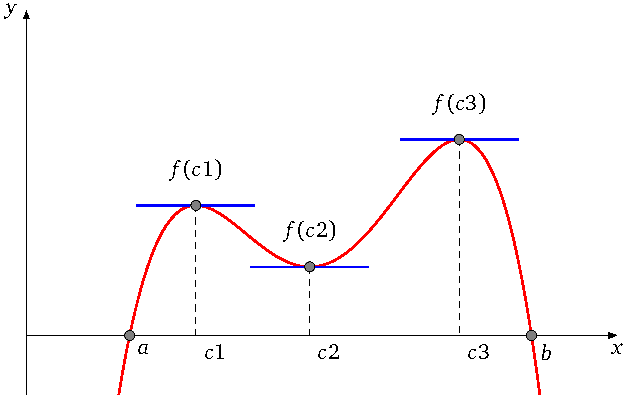
\includegraphics[scale=0.8]{25_home_antalcides_Calculo_pdf_Tikzfile47.pdf}\caption{Extremos locales}

\label{figad1}%
\end{minipage}
\end{figure}

\begin{defi}{M�ximo local}{ml}

Sea $f:\;D_{f}\subseteq\mathbb{R}\longrightarrow\mathbb{R}$ se dice
que $f$ alcanza un m�ximo local o relativo en $x_{0}\in D_{f}$ si,
para alg�n $\delta>0$, vale que $f\left(x_{0}\right)\geq f\left(x\right)$
para todo $x\in[D_{f}\cap\left(x_{0}-\delta,x_{0}+\delta\right)]$

\end{defi}

En la figura \ref{figad1} los puntos $B$ y $D$ son m�ximos relativos
de $f$.

\begin{defi}{M�nimo local}{ml}

Sea $f:\;D_{f}\subseteq\mathbb{R}\longrightarrow\mathbb{R}$ se dice
que $f$ alcanza un m�ximo local o relativo en $x_{0}\in D_{f}$ si,
para alg�n $\delta>0$, vale que $f\left(x_{0}\right)\leq f\left(x\right)$
para todo $x\in[D_{f}\cap\left(x_{0}-\delta,x_{0}+\delta\right)]$

\end{defi}

En ambos casos se dice que $f$ alcanza un extremo local.

\begin{figure}[H]
\noindent\begin{minipage}[b]{1\columnwidth}%
\centering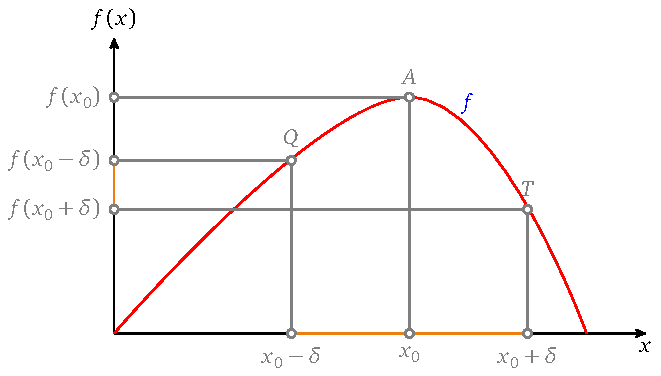
\includegraphics[scale=0.7]{26_home_antalcides_Calculo_pdf_Tikzfile20.pdf}\hfill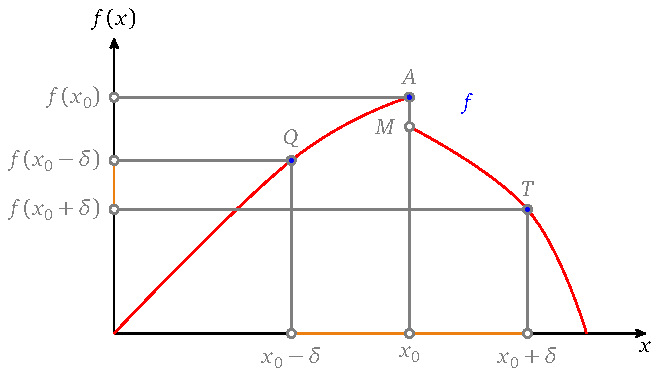
\includegraphics[scale=0.7]{27_home_antalcides_Calculo_pdf_Tikzfile21.pdf}

\caption{M�ximo local}

\label{figad2}%
\end{minipage}\vfill%
\begin{minipage}[b]{0.9\columnwidth}%
El punto $\left(x_{0},f\left(x_{0}\right)\right)$ en cada una de
las gr�ficas \ref{figad2} es un m�ximo local de $f$. por que existe
un $\delta>0$ tal que $f\left(x_{0}-\delta\right)<f\left(x_{0}\right)$
y $f\left(x_{0}+\delta\right)<f\left(x_{0}\right)$ para un intervalo
$D_{f}\cap\left(x_{0}-\delta,x_{0}+\delta\right)=\left(x_{0}-\delta,x_{0}+\delta\right)$.%
\end{minipage}
\end{figure}

\begin{figure}[H]
\noindent\begin{minipage}[b]{1\columnwidth}%
\centering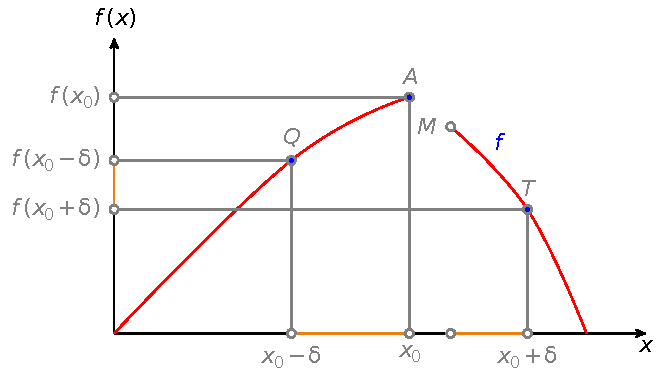
\includegraphics[scale=0.7]{28_home_antalcides_Calculo_pdf_Tikzfile22.pdf}\hfill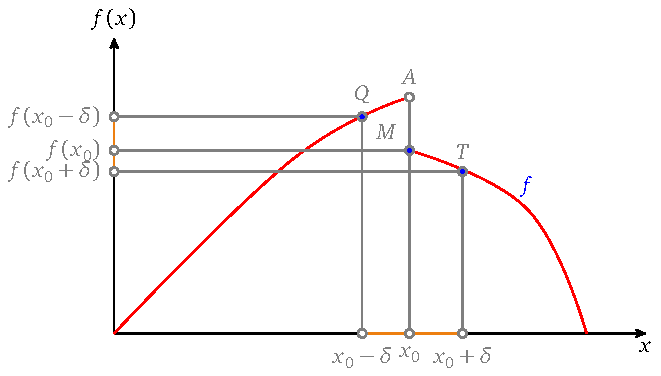
\includegraphics[scale=0.7]{29_home_antalcides_Calculo_pdf_Tikzfile23.pdf}

\caption{No hay m�ximo local}

\label{figad3}%
\end{minipage}

\begin{minipage}[b]{0.9\columnwidth}%
En este caso el punto $\left(x_{0},f\left(x_{0}\right)\right)$ en
la gr�fica de la izquierda de \ref{figad3} no es un m�ximo local
de $f$. por que no existe un $\delta>0$ tal que $f\left(x_{0}-\delta\right)<f\left(x_{0}\right)$
y $f\left(x_{0}+\delta\right)<f\left(x_{0}\right)$ para un intervalo
$D_{f}\cap\left(x_{0}-\delta,x_{0}+\delta\right)$. Ya que existen
valores $x\in\left(x_{0}-\delta,x_{0}+\delta\right)$ que no pertenecen
al $D_{f}$. Es decir la condici�n $D_{f}\cap\left(x_{0}-\delta,x_{0}+\delta\right)$
nos asegura que existen $x\in D_{f}$ y est�n muy cerca de $x_{0}.$

En la gr�fica de la derecha tampoco hay extremo relativo ya que existen
puntos como por ejemplo $Q$ donde $f\left(x_{0}-\delta\right)>f\left(x_{0}\right)$
y $T$ donde $f\left(x_{0}+\delta\right)<f\left(x_{0}\right)$.%
\end{minipage}
\end{figure}

\vspace{1cm}

\begin{teo}{Fermat}{fermat}

Sea $f$ una funci�n definida en $\left(a,b\right)$ tal que $f$
alcanza un extremo local en $x_{0}\in\left(a,b\right)$. Si $f$ es
derivable en $x_{0}$, entonces $f'\left(x_{0}\right)=0$

\end{teo}

\begin{prueba}

Como $f$ alcanza un extremo local en $x_{0}$ suponemos que este
es un m�ximo local, entonces para alg�n $\delta>0$ tenemos que vale
que $f\left(x\right)\leq f\left(x_{0}\right)$ para todo $x\in\left(x_{0}-\delta,x_{0}+\delta\right)$
y como $f$ es derivable en $x_{0}$ entonces ${\displaystyle \lim_{x\rightarrow x_{0}}\dfrac{f\left(x\right)-f\left(x_{0}\right)}{x-x_{0}}=f'\left(x_{0}\right)}$esto
asegura tambi�n la existencia de las derivadas laterales por tanto
se tiene que:
\begin{description}
\item [{i)}] para $x\rightarrow x_{0}^{-}$ se tiene $x<x_{0}$, entonces
$\dfrac{f\left(x\right)-f\left(x_{0}\right)}{x-x_{0}}\geq0$, pues
$f\left(x\right)-f\left(x_{0}\right)\leq0$ y $x-x_{0}>0$ luego ${\displaystyle f'\left(x\right)=\lim_{x\rightarrow x_{0}^{+}}\dfrac{f\left(x\right)-f\left(x_{0}\right)}{x-x_{0}}\geq0}$.
\item [{ii)}] para $x\rightarrow x_{0}^{+}$ se tiene $x>x_{0}$, entonces
$\dfrac{f\left(x\right)-f\left(x_{0}\right)}{x-x_{0}}\leq0$, pues
$f\left(x\right)-f\left(x_{0}\right)\leq0$ y $x-x_{0}<0$ luego ${\displaystyle f'\left(x\right)=\lim_{x\rightarrow x_{0}^{-}}\dfrac{f\left(x\right)-f\left(x_{0}\right)}{x-x_{0}}\leq0}$.
\end{description}
De i) y ii) se deduce que $f'\left(x_{0}\right)=0.$

\end{prueba}

La demostraci�n para el caso de un m�nimo local es id�ntica por lo
que queda de ejercicio.

\textbf{\textcolor{blue}{Nota:}} El resultado anterior es uno de los
que peor se interpretan debido a que suelen olvidarse sus hip�tesis,
que son dos:

$\bullet$\ Que en el punto $x=x_{0}$ exista un extremo relativo
de $f$.\marginpar{\flushright\curvasr}\\
\indent $\bullet$\ Que $f$ sea derivable en $x=x_{0}$.

La expresi�n ``como $f$ tiene un extremo en $x_{0}$, su derivada
debe anularse en $x=x_{0}$'' no es, en general, correcta. Los siguientes
ejemplos lo dejan bien claro: 

\begin{ejemplo}

\begin{figure}[H]
\parbox[c][1\totalheight][s]{0.4\columnwidth}{%
La funci�n \func{f}{{[}-1,1{]}}\ dada por $f(x)=x^{3}$, es
estrictamente creciente, y su derivada es $f'\left(x\right)=3x^{2}$
por lo que es derivable en todo punto y su derivada solamente se anula
en $x=0$. Tiene un m�nimo absoluto en $-1$ y un m�ximo absoluto
en $1$; dichos puntos no son extremos relativos de la funci�n, como
se puede observar en la gr�fica \ref{figad4}. La funci�n $f$ no
tiene extremos locales. Este ejemplo tambi�n muestra que la condici�n
necesaria de extremo relativo no es suficiente. 

.%
}\hfill%
\begin{minipage}[c]{0.5\columnwidth}%
\centering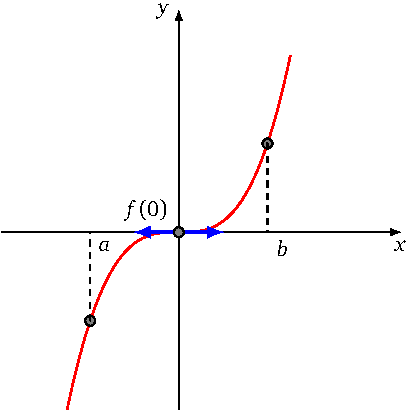
\includegraphics[scale=0.7]{30_home_antalcides_Calculo_pdf_Tikzfile48.pdf}\caption{Teorema de Fermat}

\label{figad4}%
\end{minipage}
\end{figure}

\end{ejemplo}

Otro problema del teorema de Fermat es que la funci�n debe ser derivable
en $\left(a,b\right)$ por ejemplo la funci�n $f\left(x\right)=\left|x\right|$
tiene un m�nimo local en $x=0,$ como se puede observar en la gr�fica
\ref{figad5}, pero no es derivable en $x=0.$

Es decir La funci�n \func{f}{\R}\ dada por $f(x)=\abs{x}$,
tiene claramente un m�nimo relativo (y tambi�n absoluto) en $0$,
pero no es derivable en $0$, por lo que no tiene ning�n sentido decir
que su derivada se anula en $0$. 
\begin{figure}[H]
\centering

\caption{Valor absoluto}
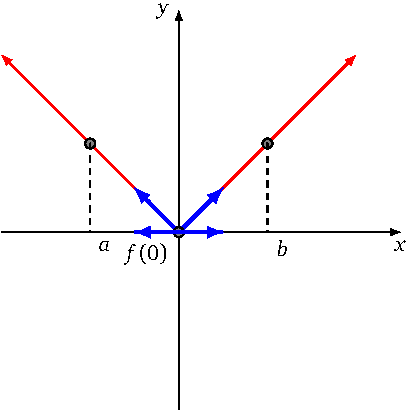
\includegraphics[scale=0.55]{31_home_antalcides_Calculo_pdf_Tikzfile49.pdf}\label{figad5}

\end{figure}
Del ejemplo anterior podemos concluir que pueden existir extremos
relativos en puntos donde la derivada no exista.

\begin{apunte} Esta condici�n $f'\left(x_{0}\right)=0$ no asegura
que $f$ tenga un extremo local en $x_{0}$, lo que asegura que si
$f$ alcanza un extremo relativo en $\left(a,b\right)$, lo alcanza
en valores $x_{0}\in\left(a,b\right)$ donde $f'\left(x_{0}\right)=0.$\end{apunte}

\subsection{Extremos globales o absolutos}

\begin{defi}{Extremos globales}{eg}

Sea $f\,:\,D_{f}\subseteq\mathbb{R}\rightarrow\mathbb{R}$ una funci�n.
Se dice que $f$ alcanza un m�ximo global o absoluto en $x_{M}\in D_{f}$
si se tiene que $f\left(x_{M}\right)\geq f\left(x\right)$ para todo
$x\in D_{f}$ y alcanza un m�nimo global o absoluto en $x_{m}\in D_{f}$
se se tiene que $f\left(x_{m}\right)\leq f\left(x\right)$ para todo
$x\in D_{f}.$ 

\end{defi}

\begin{ejemplo}

\begin{figure}[H]
\parbox[c][1\totalheight][s]{0.4\columnwidth}{%
No toda funci�n tiene extremos globales, por ejemplo $f\,:\,\left[-4,4\right]\rightarrow\mathbb{R}$
definida:
\[
f\left(x\right)=\left\{ \begin{array}{c}
\dfrac{1}{x-1},\,\,x\neq1\\
0,\,\:\qquad x=0
\end{array}\right.
\]
%
}\hfill%
\begin{minipage}[c]{0.5\columnwidth}%
\centering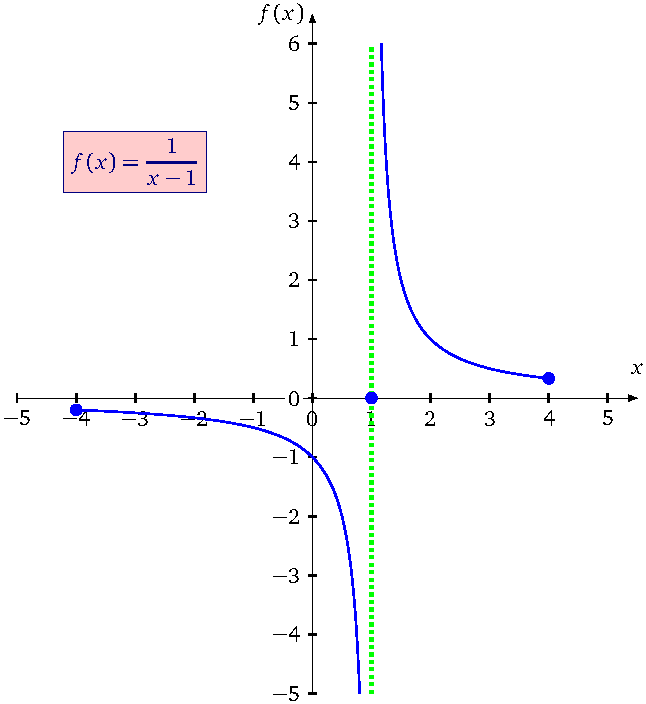
\includegraphics[scale=0.4]{32_home_antalcides_Calculo_pdf_Tikzfile51.pdf}\caption{No hay extremos globales}

\label{figad6}%
\end{minipage}
\end{figure}

\end{ejemplo}

\begin{teo}{}{}

Sea $f\,:\,\left[a,b\right]\rightarrow\mathbb{R}$ una funci�n continua
entonces $f$ est� acotada en $\left[a,b\right],$ es decir existen
n�meros reales $M$ y $m$ tales que 

$m\leq f\left(x\right)\leq M$ para todo $x\in\left[a,b\right]$

\end{teo}

\begin{ejemplo}

\begin{figure}[H]
\parbox[c][1\totalheight][s]{0.4\columnwidth}{%
Sea $f\,:\,\left[1,3\right]\rightarrow\mathbb{R}$ tal que $f\left(x\right)=x^{3}-12x+15$.
Hallar los extremos globales en $\left[1,3\right]$%
}\hfill%
\begin{minipage}[c]{0.5\columnwidth}%
\centering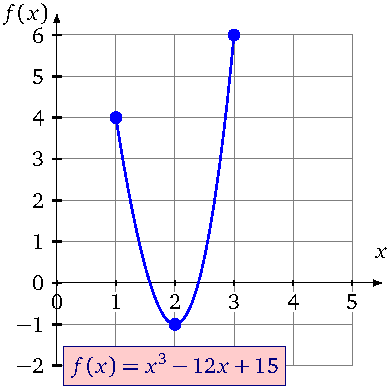
\includegraphics[scale=0.6]{33_home_antalcides_Calculo_pdf_Tikzfile52.pdf}\caption{Extremos globales}

\label{figad7}%
\end{minipage}
\end{figure}

\end{ejemplo}

\begin{solucion}

Como $f$ es continua en $\left[1,3\right]$ y derivable en $\left(1,3\right)$entonces
$f$ alcanza los extremos en $\left[1,3\right]$y se tienen dos posibilidades
\begin{description}
\item [{i)}] Por el teorema de Fermat $f$ tiene extremos en $\left(1,3\right)$
donde $f'\left(x\right)=0.$
\item [{ii)}] $f$ tiene los extremos en $x=1$ o $x=3.$
\end{description}
Entonces hallemos los ceros de la derivada $f'\left(x\right)=3x^{2}-12=0$,
por tanto $x^{2}=4$ es decir $x=\pm2.$

De lo que se deduce que hay tres valores posibles para $x$ son $1,2$
y $3$. As�:

\begin{eqnarray*}
f\left(1\right) & = & 4\\
f\left(2\right) & = & -1\\
f\left(3\right) & = & 6
\end{eqnarray*}
de estos resultados se concluye que en $x=2$ hay un m�nimo absoluto
y en $x=3$ hay un m�ximo absoluto.

\end{solucion}

\subsection{Teorema de Rolle y del valor medio}

Los resultados m�s �tiles del c�lculo diferencial se refieren a funciones
derivables en todos los puntos de un intervalo. El teorema del valor
medio es frecuentemente atribuido a Joseph Louis Lagrange; no obstante,
fue publicado por vez primera en 1806 por el f�sico Andr� Marie Amp�re
que justificaba el resultado usando ideas de Lagrange y suponiendo
que la funci�n derivada era continua; lo cual, como se ver� enseguida,
es innecesario. Quince a�os m�s tarde Augustin Cauchy volvi� a probar
el teorema con las mismas hip�tesis. El teorema del valor medio es
uno de los resultados m�s �tiles del C�lculo. Su utilidad se debe
principalmente a que dicho teorema permite acotar el incremento de
una funci�n cuando se conoce una cota de su derivada.

Michel Rolle (1652 - 1719) fue miembro de la Acad�mie des Sciences
y en 1691, estudiando un m�todo para resolver ecuaciones, estableci�,
sin demostrar, el teorema que ahora lleva su nombre que, como veremos,
es esencialmente equivalente al teorema del valor medio.

\begin{teo}{Rolle}{rolle} Sea $f\,:\,\left[a,b\right]\rightarrow\mathbb{R}$
una funci�n continua en un intervalo $\left[a,b\right]$ y derivable
en el intervalo abierto $\left(a,b\right)$ . Si $f\left(a\right)=f\left(b\right)$
entonces existe un valor $c\in\left(a,b\right)$ tal que $f'\left(c\right)=0.$ 

\end{teo}

\begin{figure}[H]

\caption{Teorema de Rolle}
\centering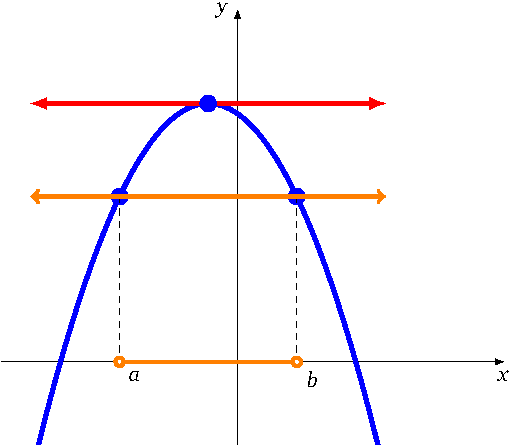
\includegraphics[scale=0.5]{34_home_antalcides_Calculo_pdf_Tikzfile53.pdf}\label{figad8}

\end{figure}

\vspace*{10mm}

\dem La continuidad de $f$ en $[a,b]$ garantiza que $f$ alcanza
en un punto %
\mbox{%
$u\en[a,b]$%
} un m�nimo absoluto y en un punto $v\en[a,b]$ un m�ximo absoluto.
Si $\{u,v\}=\{a,b\}$, entonces ser�\linebreak{}
\begin{figure}[h]
\centering{}%
\begin{minipage}[t]{0.55\textwidth}%
\vspace{-10pt}
 \hspace{5mm}  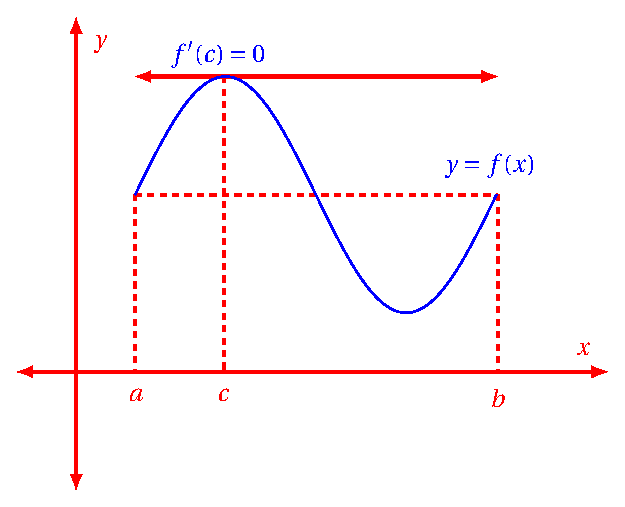
\includegraphics[scale=0.5]{35_home_antalcides_Calculo_pdf_Tikzfile40.pdf}\captionsetup{,singlelinecheck=off,margin=1cm}
\caption{Teorema de Rolle}
%
\end{minipage}%
\begin{minipage}[t]{0.45\textwidth}%
 \vspace{-16pt}
 $f(u)=f(v)$ y, por tanto $f$ es constante en $[a,b]$ y, en consecuencia,
su derivada es nula. Si $\{u,v\}\neq\{a,b\}$, entonces alguno de
los puntos $u$, $v$ est� en $]a,b[$ y es un extremo relativo de
$f$ por lo que, en virtud de la proposici�n anterior, concluimos
que la derivada de $f$ se anula en alg�n punto de $]a,b[$.\fin %
\end{minipage}
\end{figure}

\vspace*{1mm}

\noindent \textbf{Observaciones.} Observa que la demostraci�n del
teorema de Rolle que hemos dado, que es la usual, depende de forma
esencial del teorema de Weierstrass \ref{th:teoremadeweierstrass}
que garantiza la existencia de valores extremos absolutos.

El enunciado anterior del teorema de Rolle es el usual; pero, en cierto
sentido, es ``demasiado preciso''. Esto se debe a que las hip�tesis
que se consideran en el teorema son las m�nimas indispensables. Por
ejemplo, si consideramos la funci�n \func{f}{{[}-1,1{]}}\ dada
por $f(x)=\sqrt{1-x^{2}}$, cuya gr�fica es la mitad superior de la
circunferencia unidad, se tiene que $f$ es continua en $[-1,1]$,
derivable en $]-1,1[$ y, claro est�, su derivada se anula en $x=0$.
Esta funci�n no es derivable en los extremos del intervalo. Pero la
situaci�n m�s corriente es que la funci�n sea derivable en todo el
intervalo, incluidos sus extremos. Adem�s, es frecuente trabajar con
funciones definidas en intervalos abiertos que no tienen puntos extremos,
en cuyo caso debemos elegir un intervalo apropiado para aplicar el
teorema.

El teorema de Rolle se usa para estudiar ra�ces de ecuaciones, pues
permite relacionar los ceros de una funci�n derivable con los de su
derivada. Un cero de una funci�n es, naturalmente, un punto en el
que la funci�n se anula.

\begin{coro}{Rolle}{cerosrolle} a) Entre cada dos ceros de una funci�n
derivable en un intervalo hay por lo menos un cero de su derivada.

b) Entre cada dos ceros \emph{consecutivos} de la derivada de una
funci�n en un intervalo, solamente puede haber, como mucho, un cero
de la funci�n; o puede que la funci�n no tenga ning�n cero entre los
dos ceros de su derivada. \end{coro}

\dem \emph{a)} Sea \func{f}{I}\ una funci�n derivable en un
intervalo $I$. Sean $a,b\in I$ tales que $f(a)=f(b)=0$. El teorema
de Rolle nos dice que hay alg�n punto entre $a$ y $b$ en el que
se anula la derivada de $f$.

\noindent \emph{b)} Supongamos que $s,t$ son ceros \emph{consecutivos}
de la derivada de $f$, esto es, $f\tl(s)=f\tl(t)=0$ y $f\tl$ no
se anula en ning�n punto comprendido entre $s$ y $t$. En tal caso
puede ocurrir que $f$ no tenga ning�n cero comprendido entre $s$
y $t$ o que tenga solamente uno. No puede ocurrir que $f$ tenga
m�s de un cero entre $s$ y $t$, pues en tal caso su derivada tendr�a
que anularse en alg�n punto comprendido entre $s$ y $t$, cosa que
no sucede.\fin

El apartado \emph{b)} suele expresarse diciendo que \emph{los ceros
de la derivada separan los ceros de la funci�n}. Debes entender bien
lo que se afirma en \emph{b)}. Por ejemplo, puede ocurrir que la derivada
se anule en varios puntos y la funci�n no se anule nunca: la funci�n
$f(x)=2+\sen x$ no se anula nunca, pero su derivada $f\tl(x)=\cos x$
tiene infinitos ceros.

\begin{teo}{Lagrange}{lagrange} Sea $f\,:\,\left[a,b\right]\rightarrow\mathbb{R}$
una funci�n continua en un intervalo cerrado $\left[a,b\right]$ y
derivable en $\left(a,b\right)$entonces existe un valor $c\in\left(a,b\right)$
tal que $f'\left(c\right)=\dfrac{f\left(b\right)-f\left(a\right)}{b-a}$

\end{teo}

\begin{figure}[H]
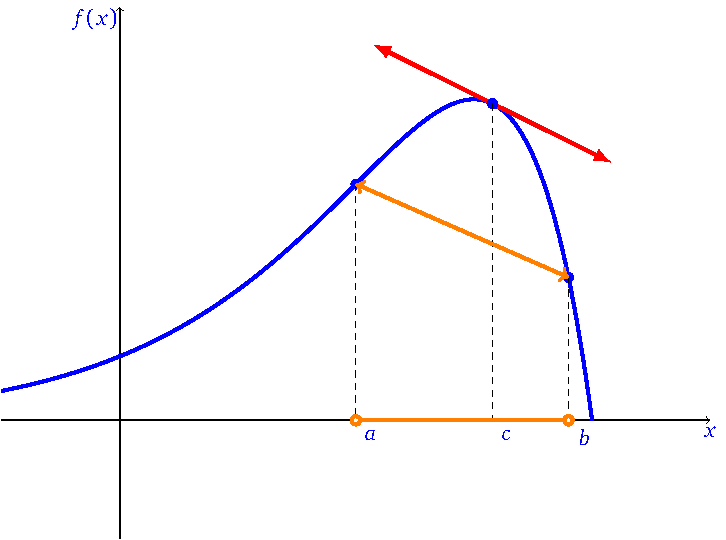
\includegraphics[scale=0.5,bb = 0 0 200 100, draft, type=eps]{/media/antalcides/Antalcides-EXT/maletin/apuntes/calculo/pdf/Tikzfile54.pdf}

\caption{Teorema del valor medio o de Lagrange}
\end{figure}

\dem Definamos una funci�n \func{g}{{[}a,b{]}}\ por $g(x)=f(x)+\lambda x$
donde $\lambda$ lo elegiremos por la condici�n de que $g(a)=g(b)$,
es decir: 
\[
f(a)+\lambda a=f(b)+\lambda b\quad\longrightarrow\quad\lambda=-\dfrac{f(b)-f(a)}{b-a}
\]
Podemos aplicar ahora el teorema de Rolle en el intervalo $[a,b]$
a la funci�n 
\[
g(x)=f(x)-\dfrac{f(b)-f(a)}{b-a}x
\]
para deducir que hay un punto $c\in]a,b[$ tal que 
\[
g\tl(c)=f\tl(c)-\dfrac{f(b)-f(a)}{b-a}=0
\]
lo que concluye la demostraci�n.\fin 
\noindent \begin{center}
\begin{figure}[H]
\centering 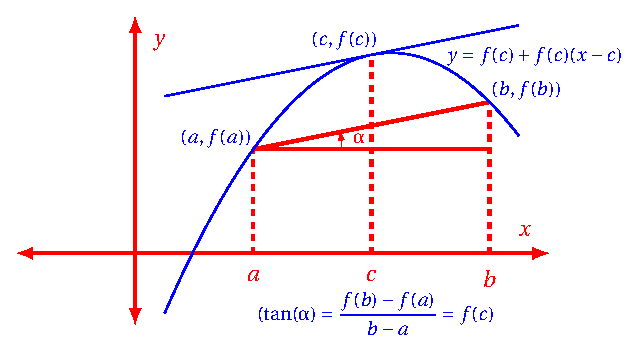
\includegraphics[scale=0.7]{36_home_antalcides_Calculo_pdf_lagrange.pdf}\caption{Teorema del valor medio}
\end{figure}
\par\end{center}

Lo que afirma el teorema del valor medio es que el incremento medio
de una funci�n en un intervalo es igual a su derivada o ``incremento
puntual'' en alg�n punto del mismo. Geom�tricamente: la tangente
a la gr�fica de $f$ en alg�n punto $c$ comprendido entre $a$ y
$b$ es paralela a la cuerda que une los puntos $(a,f(a)$ y $(b,f(b))$.

Observa que el teorema del valor medio lo hemos deducido del teorema
de Rolle, pero es evidente que el teorema de Rolle puede deducirse
del teorema del valor medio. Son dos resultados equivalentes. En lo
que sigue nos referiremos al teorema del valor medio por las siglas
TVM. 

\subsubsection{Consecuencias del teorema del valor medio}

\begin{proposicion}{}{} Sea $f$ una funci�n derivable en un intervalo
$I$, y supongamos que existe $M\geqslant0$ tal que $|f\tl(x)|\leqslant M$
para todo $x\en I$. Entonces se verifica que 
\begin{equation}
|f(x)-f(y)|\leqslant M|x-y|\qquad\textrm{para todos }x,y\en I\label{desigualdadTVM}
\end{equation}
En particular, si $f\tl(x)=0$ para todo $x\en I$ entonces $f$ es
constante en $I$. \end{proposicion} \dem Dados $x,y\en I$, el
TVM aplicado a la funci�n $f$ en el intervalo de extremos $x$ e
$y$ nos dice que hay alg�n punto $z$ en dicho intervalo tal que
$f(x)-f(y)=f\tl(z)(x-y)$. Tomando valores absolutos tenemos 
\[
\abs{f(x)-f(y)}=\abs{f\tl(z)}\abs{x-y}\leq M\abs{x-y}
\]
Si la derivada de $f$ es id�nticamente nula en $I$ podemos tomar
$M=0$ en la desigualdad (\ref{desigualdadTVM}) para obtener que
$f(x)=f(y)$ para todos $x,y\en I$, lo que nos dice que $f$ es constante
en $I$.\fin

El resultado anterior, adem�s de su inter�s te�rico, es muy �til para
probar desigualdades.

En la proposici�n anterior la hip�tesis de que $I$ es un intervalo
es esencial. La funci�n \func{f}{{]}0,1{[}\cup{]}1,2{[}}\ dada
por $f(x)=1$ si $0<x<1$ y $f(x)=2$ si $1<x<2$, es derivable en
todo punto con derivada nula y no es constante.

\begin{proposicion}{}{prop:dernodisc} Sea $I$ un intervalo, $a\en I$
y $f$ una funci�n continua en $I$ y derivable en $I\backslash\{a\}$.
Si la funci�n derivada $f\tl$ tiene l�mite por la derecha (resp.
por la izquierda) en $a$ entonces $f$ es derivable por la derecha
(resp. por la izquierda) en $a$ con derivada por la derecha (resp.
por la izquierda) en $a$ igual al valor de dicho l�mite. En particular,
si existe $\dis\lim_{x\to a}f\tl(x)=L$ entonces $f$ es derivable
en $a$ y $f\tl(a)=L$. \end{proposicion} \dem Supongamos $\dis\lim_{\substack{x\to a\\
x<a
}
}f\tl(x)=L$. Dado \epos, existe $\delta>0$ tal que %
\mbox{%
$]a-\delta,a]\subset I$%
} y para $a-\delta<x<a$ se verifica que $|f\tl(x)-L|<\eps$. Dado
$x\in]a-\delta,a]$, podemos aplicar el teorema del valor medio a
la funci�n $f$ en el intervalo $[x,a]$ y deducimos que hay alg�n
punto $c\in]x,a[\subset]a-\delta,a[$ tal que $f(x)-f(a)=f\tl(c)(x-a)$
y por tanto: 
\[
\left|\frac{f(x)-f(a)}{x-a}-L\right|=|f\tl(c)-L|<\eps.
\]
Lo que prueba que 
\[
\limlft{\frac{f(x)-f(a)}{x-a}}{x}{a}=L,
\]
es decir, $f$ es derivable por la izquierda en $a$ y la derivada
por la izquierda de $f$ en $a$ es igual a $L$.

\noindent El resto de las afirmaciones del enunciado se deducen f�cilmente
de lo anterior.\fin

La proposici�n anterior tiene una interesante consecuencia que, entre
otras cosas, nos informa de que no toda funci�n puede ser la derivada
de otra.

\begin{coro}{}{cor:discontinuidadderivadas} Las funciones derivadas
definidas en intervalos no tienen discontinuidades evitables ni de
salto. \end{coro}

\begin{teo}{Cauchy}{cauchy} Sean $f$ y $g$ funciones continuas
en el intervalo cerrado $\left[a,b\right]$ y derivable en $\left(a,b\right)$.
Entonces un valor $c\in\left(a,b\right)$ tal que 
\[
f'\left(c\right)\left(g\left(b\right)-g\left(a\right)\right)=f'\left(c\right)\left(f\left(b\right)-f\left(a\right)\right)
\]
 si adem�s $g'\left(x\right)\neq0$ para todo$x\in\left(a,b\right)$
entonces 
\[
\dfrac{f\left(b\right)-f\left(a\right)}{g\left(b\right)-g\left(a\right)}=\dfrac{f'\left(c\right)}{g'\left(c\right)}.
\]

\end{teo}

\dem Definimos una funci�n $h(x)=\lambda f(x)+\mu g(x)$ donde $\lambda$,
$\mu$ son n�meros que se eligen de forma que $h(a)=h(b)$, esto es,
$\lambda(f(a)-f(b))=\mu(g(b)-g(a))$. Basta para ello tomar $\lambda=g(b)-g(a)$,
$\mu=f(a)-f(b)$. El teorema del Rolle, aplicado a la funci�n $h(x)=(g(b)-g(a))f(x)-(f(b)-f(a))g(x)$,
nos dice que hay un punto $c\in]a,b[$ tal que $h\tl(c)=0$, lo que
concluye la demostraci�n.\fin

\subsubsection{Reglas de L'H�pital}

\noindent Guillaume Fran�ois Antoine de L'H�pital (1661-1704), public�
an�nimamente en 1696 el primer libro de texto sobre c�lculo diferencial,
el cual tuvo gran �xito e influencia durante el siglo XVIII. En �l
aparecen los resultados que hoy llevan su nombre, que permiten resolver
en muchos casos indeterminaciones de la forma $\frac{0}{0}$ o $\frac{\infty}{\infty}$,
que se presentan frecuentemente al estudiar el l�mite de un cociente
de dos funciones. Si bien L'H�pital era un escritor excepcionalmente
claro y eficaz, las llamadas ``reglas de L'H�pital'' no se deben
a �l sino a su maestro Jean Bernouilli (1667-1748).

\begin{teo}{L'Hopital I}{lopital1}

Sea $I$ un intervalo, $a\in I$ y $f,g\,:\,I-\{a\}\rightarrow\mathbb{R}$
funciones que cumplen que :
\begin{lyxlist}{00.00.0000}
\item [{a.}] $f$ y $g$ son derivables en $I-\{a\}.$
\item [{b.}] $g'\left(x\right)\neq0$ para todo $x\in I-\{a\}.$
\item [{c.}] ${\displaystyle \lim_{x\rightarrow a}f\left(x\right)=\lim_{x\rightarrow a}g\left(x\right)=0}$.
\end{lyxlist}
Entonces se tiene que $g\left(x\right)\neq0$ para todo $x\in I-\{a\}$
con las funciones $\frac{f}{g}$ y $\frac{f'}{g'}$ est�n definidas
en $I-\{a\}$ y se verifica que 
\begin{description}
\item [{i)}] ${\displaystyle \lim_{x\rightarrow a}\dfrac{f'\left(x\right)}{g'\left(x\right)}=L\in\mathbb{R}\longrightarrow\lim_{x\rightarrow a}\dfrac{f\left(x\right)}{g\left(x\right)}=L}.$
\item [{ii)}] Si $\dfrac{f'}{g'}$ diverge cuando $x\rightarrow a,$ entonces
$\dfrac{f}{g}$tambi�n diverge cuando $x\rightarrow a.$
\end{description}
\end{teo}

\begin{teo}{L'Hopital II}{lopital2}

Sea $I$ un intervalo, $a\in I$ y $f,g\,:\,I-\{a\}\rightarrow\mathbb{R}$
funciones que cumplen que :
\begin{lyxlist}{00.00.0000}
\item [{a.}] $f$ y $g$ son derivables en $I-\{a\}.$
\item [{b.}] $g'\left(x\right)\neq0$ para todo $x\in I-\{a\}.$
\item [{c.}] ${\displaystyle g}$ diverge en $x=a.$
\end{lyxlist}
Entonces existe un $\rho>0$ tal que para todo $x\in I$ con $0<\left|x-a\right|<\rho$
se tiene que $g\neq0.$ Adem�s se verifica que: 
\begin{description}
\item [{i)}] ${\displaystyle \lim_{x\rightarrow a}\dfrac{f'\left(x\right)}{g'\left(x\right)}=L\in\mathbb{R}\longrightarrow\lim_{x\rightarrow a}\dfrac{f\left(x\right)}{g\left(x\right)}=L}.$
\item [{ii)}] Si $\dfrac{f'}{g'}$ diverge cuando $x\rightarrow a,$ entonces
$\dfrac{f}{g}$ tambi�n diverge cuando $x\rightarrow a.$
\end{description}
\end{teo}

\begin{teo}{L'Hopital III}{lopital3}

Sea $I$ un intervalo sin cota superior y $f,g\,:\,I\rightarrow\mathbb{R}$
funciones que cumplen que :
\begin{lyxlist}{00.00.0000}
\item [{a.}] $f$ y $g$ son derivables en $I.$
\item [{b.}] $g'\left(x\right)\neq0$ para todo $x\in I.$
\item [{c.}] ${\displaystyle \lim_{x\rightarrow+\infty}f\left(x\right)=\lim_{x\rightarrow+\infty}g\left(x\right)=0}$.
\item [{d.}] $g\rightarrow+\infty$
\end{lyxlist}
Entonces existe un $M>0$ tal que para todo $x\in I$ con $x>m,$
se tiene $g\left(x\right)\neq0$, adem�s se verifica
\begin{description}
\item [{i)}] ${\displaystyle \lim_{x\rightarrow+\infty}\dfrac{f'\left(x\right)}{g'\left(x\right)}=L\in\mathbb{R}\longrightarrow\lim_{x\rightarrow+\infty}\dfrac{f\left(x\right)}{g\left(x\right)}=L}.$
\item [{ii)}] Si $\dfrac{f'}{g'}$ diverge cuando $x\rightarrow+\infty,$
entonces $\dfrac{f}{g}$ tambi�n diverge cuando $x\rightarrow\infty.$
\end{description}
\end{teo}

\noindent Las distintas formas de las reglas de L'H�pital pueden resumirse
en el siguiente enunciado.

\begin{teo}{Jean Bernouilli}{} Sean $-\infinity\leqslant a<b\leqslant+\infinity$,
$f$ y $g$ funciones derivables en $]a,b[$ con $g\tl(x)\neq0$,
para todo $x\in]a,b[$. Sea $\alpha\en\{a,b\}$ y supongamos que se
verifica alguna de las dos condiciones siguientes: 
\begin{enumerate}
\item $\dis{\lim_{x\to\alpha}f(x)=\lim_{x\to\alpha}g(x)=0}$ 
\item $\dis{\lim_{x\to\alpha}|g(x)|=+\infinity}$ 
\end{enumerate}
Y adem�s 
\[
\lim_{x\to\alpha}\frac{f\tl(x)}{g\tl(x)}=L\en\R\cup\{+\infinity,-\infinity\}
\]
Entonces se verifica que 
\[
\lim_{x\to\alpha}\frac{f(x)}{g(x)}=L
\]
\end{teo} \dem Antes de dar una demostraci�n al uso vamos a explicar
por qu� la hip�tesis de que el cociente de las derivadas tiene l�mite
implica que tambi�n lo tiene el cociente de las funciones. Para fijar
ideas, consideremos el caso en que $\alpha=a$ es un n�mero real y
$\dis{\lim_{x\to\alpha}f(x)=\lim_{x\to\alpha}g(x)=0}$. Definamos
$f(a)=g(a)=0$.

\noindent Observa que, aunque el punto $(g(x),f(x))$ recorre una
trayectoria en el plano que termina en $(0,0)$ cuando $x=a$, el
l�mite $\rule{0mm}{5mm}\lim_{x\to a}\frac{f(x)}{g(x)}$ no tiene por
qu� existir. Ello se debe a que la proximidad a $(0,0)$ del punto
$(g(x),f(x))$ no proporciona ninguna informaci�n sobre el valor del
cociente $\rule{0mm}{5mm}\frac{f(x)}{g(x)}$. Baste considerar que
en un c�rculo centrado en $(0,0)$ de radio tan peque�o como queramos,
hay puntos $(u,v)$ para los que el cociente $\frac{u}{v}$ puede
tomar cualquier valor.

Geom�tricamente, podemos interpretar $\frac{f(x)}{g(x)}$ como la
pendiente de la recta que une $(0,0)$ con el punto $(g(x),f(x))$.
Si imaginamos que el punto $\gamma(x)=(g(x),f(x))$ recorre una curva
$\Gamma$ en el plano que termina en $(0,0)$, parece evidente que,
cuando dicho punto est� muy pr�ximo a $(0,0)$, el n�mero $\rule{0mm}{5mm}\frac{f(x)}{g(x)}$
est� muy pr�ximo a la pendiente de la tangente a $\Gamma$ en $(g(x),f(x))$.
La figura \ref{fig:hopital} puede servir de ayuda.
\begin{center}
\begin{figure}[H]
\centering 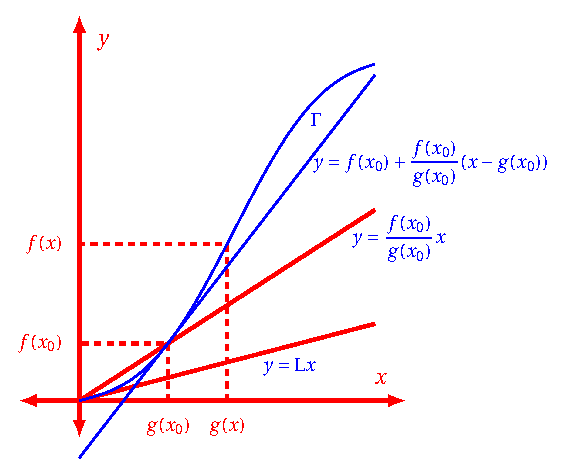
\includegraphics[scale=0.6]{37_home_antalcides_Calculo_pdf_lhopital.pdf}\caption{Regla de L'H�pital}
\label{fig:hopital} 
\end{figure}
\par\end{center}

\noindent F�jate que como $f$ y $g$ no se suponen derivables en
$x=a$, no est� garantizado que $\Gamma$ tenga tangente en el origen,
es decir, para $x=a$. Podemos, sin embargo, calcular la tangente
a $\Gamma$ en puntos distintos del origen. Para ello podemos usar
que el vector tangente a $\Gamma$ en un punto $x_{0}$ es $\gamma\tl(x_{0})=(g\tl(x_{0}),f\tl(x_{0}))$,
y la recta tangente en dicho punto tiene las ecuaciones param�tricas:
\[
(x,y)=(g(x_{0}),f(x_{0}))+\lambda(g\tl(x_{0}),f\tl(x_{0}))
\]
Eliminando el par�metro $\lambda$ en esta ecuaci�n obtenemos la ecuaci�n
cartesiana de la tangente que resulta ser 
\[
y=f(x_{0})+\frac{f\tl(x_{0})}{g\tl(x_{0})}(x-g(x_{0}))
\]
Lo que nos dice que la pendiente de dicha tangente es $\frac{f\tl(x_{0})}{g\tl(x_{0})}$.
En consecuencia, la pendiente de la tangente a $\Gamma$ en un punto
gen�rico $x\neq a$ es $\frac{f\tl(x)}{g\tl(x)}$.

A la vista de lo anterior, se comprende ahora que si exigimos que
$\frac{f\tl(x)}{g\tl(x)}$ tenga l�mite $L$ en el punto $a$, estamos
obligando a que el cociente $\frac{f(x)}{g(x)}$ tambi�n tenga l�mite
igual a $L$ en $a$. En la figura se ha supuesto que $L$ es un n�mero
real, pero est� claro que puede suponerse tambi�n $L=\pm\infinity$
lo que corresponde a los casos en que $\Gamma$ tiene tangente vertical
en el origen.

Daremos ahora una demostraci�n formal del teorema en dos casos particulares.

\noindent \textbf{Caso1} (Primera regla de L'H�pital).

\noindent Supongamos que $\alpha=a$ y $L$ son n�meros reales y $\dis{\lim_{x\to a}f(x)=\lim_{x\to a}g(x)=0}$.
Definamos %
\mbox{%
$f(a)=g(a)=0$.%
} Dado $x\en I$, $x\neq a$, aplicamos el teorema del valor medio
generalizado a las funciones $f$ y $g$ en el intervalo $[a,x]$,
para obtener $c_{x}\in]a,x[$ tal que 
\[
(f(x)-f(a))g\tl(c_{x})=(g(x)-g(a))f\tl(c_{x})
\]
es decir, %
\mbox{%
$f(x)g\tl(c_{x})=g(x)f\tl(c_{x})$.%
} Las hip�tesis hechas implican que $g$ es estrictamente mon�tona
en $I$ y, como $g(a)=0$, deducimos que $g(x)\neq0$ para todo $x\en I$.
Obtenemos as� que: 
\begin{equation}
\frac{f(x)}{g(x)}=\frac{f\tl(c_{x})}{g\tl(c_{x})}.\label{tvg}
\end{equation}
Por hip�tesis, dado \epos, existe $\delta>0$ tal que para $a<t<a+\delta$
es $\dis{\left|\frac{f\tl(t)}{g\tl(t)}-L\right|<\eps}$. Deducimos
de la igualdad \eqref{tvg} que si $a<x<a+\delta$ se tiene que: 
\[
\left|\frac{f(x)}{g(x)}-L\right|<\eps.
\]
Hemos probado as� que $\Lim{f(x)/g(x)}{x}{a}=L$. Los casos en que
$L=\pm\infinity$ se tratan de la misma forma.

\sskip

\noindent \textbf{Caso 2} (Segunda Regla de L'H�pital).

\noindent Supongamos que $\alpha=a$ y $L$ son n�meros reales y $\Lim{|g(x)|}{x}{a}=+\infinity$.
Esta �ltima condici�n implica que $g(x)\neq0$ para todo $x\en I$
suficientemente pr�ximo al punto $a$, y por el car�cter local del
l�mite no es restrictivo suponer que $g(x)\neq0$ para todo $x\en I$.
N�tese tambi�n que las hip�tesis hechas implican que $g$ es inyectiva
en $I$. La hip�tesis $\dis\lim_{x\to a}f\tl(x)/g\tl(x)=L$, nos dice
que dado \epos, hay un n�mero (fijo en lo que sigue) $c\en I$, tal
que para $a<t\leqslant c$ se verifica que: 
\begin{equation}
\left|\frac{f\tl(t)}{g\tl(t)}-L\right|<\frac{\eps}{4}\label{eqprime}
\end{equation}
Como $\Lim{|g(x)|}{x}{a}=+\infty$, hay un n�mero $\delta>0$ tal
que $a+\delta\leqslant c$ y para $a<x<a+\delta$ se verifica que:
\begin{equation}
\frac{|g(c)|}{|g(x)|}<1,\quad\frac{|f(c)-Lg(c)|}{|g(x)|}<\frac{\eps}{2}\label{eqsecd}
\end{equation}
Dado $a<x<a+\delta$ aplicamos el teorema del valor medio generalizado
para obtener un punto $c_{x}\in]x,c[$ tal que 
\[
\frac{f(x)-f(c)}{g(x)-g(c)}=\frac{f\tl(c_{x})}{g\tl(c_{x})}.
\]
Teniendo en cuenta la identidad: 
\begin{align*}
\dis\frac{f(x)}{g(x)}-L & =\dis{\left(\frac{f(x)-f(c)}{g(x)-g(c)}-L\right)\left(1-\frac{g(c)}{g(x)}\right)+\frac{f(c)-Lg(c)}{g(x)}}\\
 & =\dis{\left(\frac{f\tl(c_{x})}{g\tl(c_{x})}-L\right)\left(1-\frac{g(c)}{g(x)}\right)+\frac{f(c)-Lg(c)}{g(x)}}
\end{align*}
deducimos, en virtud de \eqref{eqprime} y \eqref{eqsecd}, que para
todo $x\in]a,a+\delta[$ se verifica que: 
\[
\left|\frac{f(x)}{g(x)}-L\right|\leqslant\frac{\eps}{4}2+\frac{\eps}{2}=\eps.
\]
Hemos probado as� que $\Lim{f(x)/g(x)}{x}{a}=L$. Los casos en que
$L=\pm\infinity$ se tratan de la misma forma.

Los dem�s casos tienen un tratamiento similar y tambi�n pueden reducirse
a los ya estudiados sin m�s que invertir la variable.\fin

N�tese que, tal y como las hemos enunciado, las reglas de L'H�pital
permiten calcular l�mites por la derecha y por la izquierda en un
punto y, por tanto, podemos usarlas para calcular el l�mite en un
punto de un intervalo que no sea extremo del mismo.

\subsubsection{T�cnicas para calcular l�mites de funciones}

Cuando en un ejercicio te piden calcular un l�mite, es casi seguro
que se trata de una \emph{``indeterminaci�n''}. Te recuerdo que
aquellos l�mites de sumas, productos, cocientes o potencias de funciones
en los que el resultado no est� predeterminado por el comportamiento
particular de cada una de las funciones se llaman \emph{``l�mites
indeterminados''}. La palabra \emph{``indeterminado''} quiere decir
simplemente que se trata de l�mites cuyo c�lculo no puedes hacerlo
aplicando las reglas b�sicas del \emph{``�lgebra de l�mites''} y
tienes que usar alguna t�cnica apropiada para calcularlos. Los l�mites
\emph{interesantes} son casi siempre de este tipo.

Las reglas de L'H�pital son muy �tiles para resolver las indeterminaciones,
pero yo pienso que se abusa de ellas. Las aplicamos sin pensar dos
veces lo que hacemos, nos dejamos llevar por la comodidad que proporcionan
(aunque no siempre) y acabamos calculando l�mites de forma mec�nica
sin saber muy bien qu� es lo que hacemos. No tengo nada en contra
de ellas, tan s�lo me parece que su uso casi exclusivo y de forma
mec�nica es empobrecedor. Por el contrario, pienso que cada l�mite
debe intentarse de la forma m�s adecuada a su caso. Para eso tienes
que fijarte en c�mo es la funci�n, relacionarla con otras parecidas
y tratar de relacionar el l�mite que te piden con otros bien conocidos.

Voy a contarte las estrategias que suelo usar para calcular l�mites.
Esencialmente, puedo resumirlas en dos:

$\bullet$ Trato de reducir el l�mite a otros bien conocidos.

$\bullet$ Siempre que puedo sustituyo funciones por otras m�s sencillas.

Vayamos con la primera. Si te preguntas qu� entiendo por l�mites \emph{bien
conocidos}, la respuesta es bien f�cil: los que siguen a continuaci�n. 

\paragraph{L�mites que debes saberte de memoria}

\begin{apunte}
$$ 
\begin{array}{llll} 
\Lim{\dfrac{\sen x}{x}}{x}{0}=1, & \Lim{\dfrac{\arcsen x}{x}}{x}{0}=1, & \Lim{\dfrac{\arctg x}{x}}{x}{0}=1, & \Lim{\dfrac{1-\cos x}{x^2}}{x}{0}=\dfrac{1}{2},  
\\ \rule{0mm}{8mm} \Lim{\dfrac{e^x -1}{x}}{x}{0}=1, & 
\Lim{\dfrac{(1+x)^\alpha -1}{x}}{x}{0}=\alpha, & 
\Lim{\dfrac{\log(1+x)}{x}}{x}{0}=1, & 
\Lim{\dfrac{x-\sen x}{x^{3}}}{x}{0}=\dfrac{1}{6}, \\ \rule{0mm}{8mm} \Lim{\dfrac{\log x}{x-1}}{x}{1}=1, & \Lim{\dfrac{\tg x - x}{x^{3}}}{x}{0}=\dfrac{1}{3}, & \Lim{\dfrac{\tg x}{x}}{x}{0}=1, & \Lim{\dfrac{x-\log(1+x)}{x^2}}{x}{0}=\dfrac{1}{2}.  
\end{array}
$$
\end{apunte}

Observa que todos ellos, con la excepci�n de cuatro, son \emph{derivadas}
en el punto $x=0$ de las respectivas funciones. Por ello no son dif�ciles
de recordar. Ahora bien, estos l�mites suelen aparecer algo disfrazados.
Realmente, m�s que como l�mites concretos, debes considerarlos como
\emph{modelos}.

\begin{ejemplo} El l�mite $$\Lim{\dfrac{\log(\cos x)}{\cos x -1}}{x}{0}$$
no est� en la lista anterior, pero responde al modelo $$\Lim{\dfrac{\log x}{x-1}}{x}{1}$$
en el que la variable $x$ se ha sustituido por la funci�n $\cos x$
y el punto $1$ por el punto $0$. 

\end{ejemplo}

\begin{ejemplo} Partimos del l�mite 
\[
\Lim{\dfrac{\tg x-x}{x^{3}}}{x}{0}=\dfrac{1}{3}
\]
Elijamos ahora cualquier funci�n \emph{continua} $g$ que se anule
en alg�n punto $c$, por ejemplo\linebreak{}
$g(x)=\e^{x}-1$ ($c=0$) o $g(x)=\log x$ ($c=1$), o $g(x)=\sqrt[3]{x}-1$
($c=1$), $\ldots$ En todos los casos se verifica que 
\[
\Lim{\dfrac{\tg(g(x))-g(x)}{g(x)^{3}}}{x}{c}=\frac{1}{3}
\]

Tenemos as� que 
\[
\Lim{\dfrac{\tg(\e^{x}-1)-\e^{x}+1}{(\e^{x}-1)^{3}}}{x}{0}=\Lim{\dfrac{\tg(\log x)-\log x}{(\log x)^{3}}}{x}{1}=\dfrac{1}{3}
\]

\end{ejemplo}

�Entiendes lo que pasa? Esto puede hacerse con cualquier l�mite. La
justificaci�n de estos resultados es el teorema \eqref{th:continuidadpermutaconlimite}
que establece que la continuidad permuta con el paso al l�mite (realmente
es una consecuencia de que la composici�n de funciones continuas es
continua). Como consecuencia, los l�mites de la lista anterior son
\emph{muchos m�s} de los que aparecen en ella. Si te acostumbras a
reconocerlos cuando vengan disfrazados podr�s ahorrarte mucho trabajo
innecesario. Para ayudarte, vamos a escribirlos de nuevo de forma
m�s general.

Sea $f$ cualquier funci�n tal que $f(x)\neq0$ y $\Lim{f(x)}{x}{a}=0$.
Entonces se verifica que:

\[
\begin{array}{lll}
\Lim{\dfrac{\sen f(x)}{f(x)}}{x}{a}=1, & \Lim{\dfrac{\arcsen f(x)}{f(x)}}{x}{a}=1, & \Lim{\dfrac{1-\cos f(x)}{f(x)^{2}}}{x}{a}=\dfrac{1}{2},\\
\rule{0mm}{8mm}\Lim{\dfrac{\e^{f(x)}-1}{f(x)}}{x}{a}=1, & \Lim{\dfrac{f(x)-\sen f(x)}{f(x)^{3}}}{x}{a}=\dfrac{1}{6}, & \Lim{\dfrac{(1+f(x))^{\alpha}-1}{f(x)}}{x}{a}=\alpha,\\
\rule{0mm}{8mm}\Lim{\dfrac{\log(1+f(x))}{f(x)}}{x}{a}=1, & \Lim{\dfrac{\tg f(x)}{f(x)}}{x}{a}=1, & \Lim{\dfrac{\arctg f(x)}{f(x)}}{x}{a}=1,\\
\rule{0mm}{8mm}\Lim{\dfrac{\tg f(x)-f(x)}{f(x)^{3}}}{x}{a}=\dfrac{1}{3}, & \Lim{\dfrac{f(x)-\log(1+f(x))}{f(x)^{2}}}{x}{a}=\dfrac{1}{2}.
\end{array}
\]

Vamos a la segunda estrategia. \emph{Sustituir funciones por otras
m�s sencillas}. Esto se basa en la proposici�n \eqref{equivalenciaasintotica}
que permite sustituir en un producto o en un cociente de funciones,
una de ellas por otra asint�ticamente equivalente. �Ojo! En una suma
no puedes, en general, hacer eso.

La lista de los l�mites \emph{bien conocidos} es, de hecho, una lista
de equivalencias asint�ticas y eso la hace m�s �til todav�a.

\begin{ejemplo} El l�mite 
\[
\Lim{\dfrac{\e^{x}-\cos\sqrt{2}x-x}{\tg\!^{3}x}}{x}{0}
\]
es una indeterminaci�n del tipo $\dfrac{0}{0}$ y puede hacerse por
L'H�pital. El problema est� en que vamos a tener que derivar por lo
menos dos veces y las derivadas de la tangente se van complicando.
Para evitarlo podemos sustituir $\tg x$ por $x$ pues $\tg x\thicksim x(x\to0)$.
Escribiendo 
\[
\dfrac{\e^{x}-\cos\sqrt{2}x-x}{\tg\!^{3}x}=\frac{x^{3}}{\tg\!^{3}x}\frac{\e^{x}-\cos\sqrt{2}x-x}{x^{3}}
\]
y teniendo en cuenta que 
\[
\Lim{\frac{x^{3}}{\tg\!^{3}x}}{x}{0}=\Lim{\left(\frac{x}{\tg x}\right)^{3}}{x}{0}=1,
\]
basta calcular 
\[
\Lim{\dfrac{\e^{x}-\cos\sqrt{2}x-x}{x^{3}}}{x}{0}.
\]
Lo que puedes hacer por L'H�pital muy f�cilmente. \end{ejemplo}

Las estrategias anteriores son las m�s b�sicas, pero hay otras un
poco m�s elaboradas. Esencialmente consisten en aplicar el teorema
de Taylor-Young para tratar de reducir ciertos l�mites al l�mite de
un cociente de dos polinomios. Bueno, sorpresa, todos los l�mites
de la lista de \emph{l�mites bien conocidos} son, sin excepci�n, casos
particulares del teorema de Taylor-Young.

Ahora despu�s te pondr� algunos ejemplos de esta forma de proceder.
Pero, para que puedas usar con comodidad este m�todo, tienes que saberte
de memoria, o ser capaz de deducirlos en poco tiempo, los polinomios
de Taylor de las funciones elementales. Adem�s, esta forma de proceder
se adapta m�s a unos casos que a otros y tan s�lo con la pr�ctica
se aprende cu�ndo conviene usarla.

\begin{ejemplo} Si tratas de calcular por L'H�pital el l�mite 
\[
\Lim{\frac{(\tg x)(\arctg x)-x^{2}}{x^{6}}}{x}{0},
\]
tendr�s que ser paciente porque necesitar�s derivar por lo menos cinco
veces, y en el numerador hay un producto cuyas derivadas se van haciendo
cada vez m�s complicadas. Ahora, si calculas los polinomios de Taylor
de orden 5 de $\tg x$ y $\arctg x$ en $a=0$, obtendr�s que 
\[
\tg x=x+\dfrac{1}{3}x^{3}+\dfrac{2}{15}x^{5}+o(x^{6}),\quad\arctg x=x-\dfrac{1}{3}x^{3}+\dfrac{1}{5}x^{5}+o(x^{6}).
\]
Observa que como se trata de funciones impares sus derivadas de orden
par en $x=0$ son nulas, por eso los polinomios anteriores son, de
hecho, los polinomios de Taylor de orden 6 y eso explica que aparezca
el t�rmino $o(x^{6})$. Deducimos que 
\[
\tg x\arctg x=x^{2}+\dfrac{2}{9}x^{6}+o(x^{7})
\]
y 
\[
\Lim{\frac{(\tg x)(\arctg x)-x^{2}}{x^{6}}}{x}{0}=\Lim{\dfrac{2/9x^{6}+o(x^{7})}{x^{6}}}{x}{0}=\dfrac{2}{9}
\]
Observa que aunque $\tg x\thicksim x$ y $\arctg x\thicksim x$ para
$x\to0$, se tiene que $\tg x\arctg x-x^{2}\thicksim\dfrac{2}{9}x^{6}$
para $x\to0$. F�jate que al calcular el producto 
\[
\tg x\arctg x=\left(x+\dfrac{1}{3}x^{3}+\dfrac{2}{15}x^{5}+o(x^{6})\right)\left(x-\dfrac{1}{3}x^{3}+\dfrac{1}{5}x^{5}+o(x^{6})\right)
\]
tan s�lo nos interesan las potencias de $x$ hasta la de orden $6$
inclusive, las dem�s potencias y los t�rminos de la forma $xo(x^{6})$,
$x^{2}o(x^{6})$, $o(x^{6})o(x^{6})$, etc. son todos ellos funciones
de la forma $o(x^{6})$ (pues al dividirlos por $x^{6}$ su l�mite
es cero), y su suma tambi�n es una funci�n de la forma $o(x^{6})$,
por lo que \emph{no es preciso calcularlos para hacer el l�mite}.
Observa que, al proceder de esta manera, tienes que calcular las 5
primeras derivadas en $x=0$ de las funciones $\tg(x)$ y $\arctg(x)$,
pero te ahorras el trabajo de derivar su producto. Si a�n tienes dudas,
calcula el l�mite por L'H�pital y compara. \end{ejemplo}

\begin{ejemplo} Se trata de calcular 
\[
\Lim{\dfrac{(\cos x-1)(\log(1+x)-x)-\dfrac{1}{4}x^{4}}{x^{5}}}{x}{0}.
\]
Tenemos que 
\[
\cos x=1-\dfrac{1}{2}x^{2}+o(x^{3}),\quad\log(1+x)=x-\dfrac{1}{2}x^{2}+\dfrac{1}{3}x^{3}+o(x^{3})
\]
luego 
\[
(\cos x-1)(\log(1+x)-x)=\dfrac{1}{4}x^{4}-\dfrac{1}{6}x^{5}+o(x^{5}),
\]
de donde se sigue que 
\[
\Lim{\dfrac{(\cos x-1)(\log(1+x)-x)-\dfrac{1}{4}x^{4}}{x^{5}}}{x}{0}=-\frac{1}{6}
\]
\end{ejemplo} 

\subsection{Sobre el mal uso de las reglas de L'H�pital}

No conviene aplicar las reglas de L'H�pital para calcular derivadas,
es decir, l�mites de la forma 
\[
\lim_{x\to a}\frac{f(x)-f(a)}{x-a}
\]
La raz�n es muy sencilla. Si para calcular el l�mite anterior usas
las reglas de L'H�pital, lo que haces es calcular el l�mite $\dis\lim_{x\to a}f\tl(x)$.
Si �ste l�mite es igual a $L$ deducimos que el anterior tambi�n es
igual a $L$. Pero �has probado m�s de lo que se ped�a! Acabas de
probar que la derivada de $f$ es continua en $a$, porque has probado
que $\lim_{x\to a}f\tl(x)=L=f\tl(a)$; y lo que se ped�a era solamente
calcular la derivada de $f$ en $a$. Esto puede que no tenga mayor
importancia o que s� la tenga. Depende de la funci�n. Veamos un ejemplo
t�pico.

\begin{ejemplo} Queremos calcular el l�mite siguiente: 
\begin{equation}
\lim_{x\to0}\frac{(1+x)^{\frac{1}{x}}-\e}{x}\label{limitnohopital}
\end{equation}
Pongamos $f(x)=\dis(1+x)^{\frac{1}{x}}$ y definamos $f(0)=\e$ (esto
se hace as� porque sabemos que $\Lim{f(x)}{x}{0}=\e$). El l�mite
\eqref{limitnohopital} no es otra cosa que la derivada de $f$ en
$0$. Para calcular dicha derivada, lo mejor es tomar logaritmos y
calcular la derivada en $0$ de la funci�n 
\[
g(x)=\log f(x)=\frac{\log(1+x)}{x},\quad g(0)=\log f(0)=1
\]
Tenemos que 
\[
\frac{g(x)-g(0)}{x}=\frac{\log(1+x)-x}{x^{2}}
\]
Este l�mite puede hacerse muy f�cilmente por L'H�pital, pero resulta
que es un l�mite b�sico, de los que debes saberte de memoria. Por
tanto: 
\[
\lim_{x\to0}\frac{g(x)-g(0)}{x}=-\dfrac{1}{2}.
\]
Concluimos, por la regla de la cadena, que $f(x)=\exp(g(x))$ es derivable
en $0$, y su derivada viene dada por $f\tl(0)=\exp\tl(g(0))g\tl(0)=-\dfrac{\e}{2}$.

Veamos lo que pasa si aplicamos L'H�pital para calcular el l�mite
\eqref{limitnohopital}. Primero, debemos comprobar que podemos aplicar
L'H�pital y para eso debemos observar que $\Lim{\dis(1+x)^{\frac{1}{x}}}{x}{0}=\e$.
Seguidamente, derivamos numerador y denominador en \eqref{limitnohopital},
y resulta que debemos calcular el l�mite siguiente: 
\[
\lim_{x\to0}(1+x)^{\frac{1}{x}}\left(\dfrac{1}{x(1+x)}-\dfrac{\log(1+x)}{x^{2}}\right)
\]
Que tambi�n puede hacerse por L'H�pital pero es un poco m�s complicado
que el anterior. \end{ejemplo}

Otro caso en el que puede no ser conveniente aplicar L'H�pital es
para calcular un l�mite de la forma: 
\[
\lim_{x\to a}\frac{f(x)-f(a)}{g(x)-g(a)}
\]
Primero es conveniente escribir 
\[
\frac{f(x)-f(a)}{g(x)-g(a)}=\dfrac{\dfrac{f(x)-f(a}{x-a}}{\dfrac{g(x)-g(a)}{x-a}}
\]
Si la funciones $f$ y $g$ son derivables en $a$ y $g\tl(a)\neq0$,
se sigue que 
\[
\lim_{x\to a}\frac{f(x)-f(a)}{g(x)-g(a)}=\dfrac{f\tl(a)}{g\tl(a)}
\]
Si aplicamos L'H�pital probaremos, sin necesidad, que las derivadas
de $f$ y $g$ son continuas en $a$, cosa que no se pide y que puede
ser m�s complicada que lo anterior.

Los errores m�s frecuentes al aplicar L'H�pital se deben a que no
se comprueban las hip�tesis cada vez que aplicamos las reglas. Es
frecuente empezar con una indeterminaci�n del tipo $\frac{0}{0}$
o $\frac{\infty}{\infty}$ y, despu�s de aplicar L'H�pital una vez,
no volver a comprobar que seguimos teniendo una indeterminaci�n. As�
que no lo olvides: cada vez que apliques L'H�pital comprueba que se
trata de una indeterminaci�n del tipo $\frac{0}{0}$ o $\frac{\infty}{\infty}$
y que la derivada del denominador no se anula. 

\subsection{Sobre el uso de la notaci�n ${\displaystyle \lim_{x\to a}}$}

La notaci�n que usamos para l�mites es tan buena que a veces te hace
ver lo que no hay. En cierto sentido la notaci�n ``tira de ti'':
basta con que escribas ``$\dis\lim_{x\to a}$'' delante de una funci�n
para que mentalmente hagas la sustituci�n $x=a$. Para comprobar esto
te propongo un juego: dime en menos de medio segundo el valor del
siguiente l�mite: 
\[
\lim_{x\to0}\frac{x}{x}
\]
�Has dudado? �Has cre�do que es una indeterminaci�n tipo $\frac{0}{0}$?
Si respondes que s� a estas preguntas es porque has hecho mentalmente
la sustituci�n $x=0$ en el cociente $\frac{x}{x}$ y has visto lo
que no hay. Porque, evidentemente, se tiene que $\frac{x}{x}=1$,
es decir, el l�mite anterior es el l�mite de la funci�n constante
igual a 1. No hay ninguna indeterminaci�n. Es un l�mite trivial. Lo
mismo pasa con el siguiente l�mite $\dis\lim_{x\to+\infty}1^{x}$.
Si te dejas llevar por la notaci�n y haces mentalmente la sustituci�n
$x=+\infty$, puedes creer que se trata de una indeterminaci�n $1^{\infty}$,
cuando no lo es porque, evidentemente, $1^{x}=1$ es la funci�n constante
igual a 1. Se pueden poner muchos m�s ejemplos.

�C�mo evitar que la notaci�n ``$\dis\lim_{x\to a}$'' ``tire de
ti'' y te lleve a ver lo que no hay? Pues no us�ndola hasta que no
hayas visto claramente lo que realmente hay. Este es un consejo importante:
\emph{antes de empezar a calcular un l�mite funcional, simplifica
todo lo que puedas la funci�n y no escribas el s�mbolo ``$\lim$''
hasta que no tengas una idea clara de c�mo vas a hacer los c�lculos.}

\subsubsection{Derivadas sucesivas. Polinomios de Taylor}

Sea $f$ una funci�n derivable en un intervalo $I$. Si la funci�n
derivada $f\tl$ tambi�n es derivable en $I$ decimos que $f$ es
{\em dos veces derivable\/} en $I$ y la funci�n $f^{\prime\prime}:=(f\tl)\tl$
se llama {\em derivada segunda\/} de $f$ en $I$. En general,
si $n\en\N$, decimos que $f$ es $n+1$ {\em veces derivable\/}
en $I$ si $f$ es $n$ veces derivable en $I$ y la funci�n derivada
de orden $n$ de $f$ en $I$, que representaremos por $f^{(n)}$,
es derivable en $I$; en cuyo caso la funci�n $f^{(n+1)}=(f^{(n)})\tl$
se llama {\em derivada de orden} $n+1$ de $f$ en $I$. Si $n$
es un n�mero natural, $n\geqslant2$, decimos que $f$ es $n$ {\em
veces derivable en un punto} $a\en I$, si $f$ es $n-1$ veces derivable
en $I$ y la funci�n $f^{(n-1)}$ es derivable en $a$. Se dice que
$f$ es una funci�n de clase $C^{n}$ en $I$ si $f$ es $n$ veces
derivable $I$ y la funci�n $f^{(n)}$ es continua en $I$. Se dice
que $f$ es una funci�n de clase $C^{\infty}$ en $I$ si $f$ tiene
derivadas de todos �rdenes en $I$. Por convenio se define $f^{(0)}=f$.

Observemos que una funci�n $f$ derivable en un punto $a$ puede ser
aproximada localmente por una funci�n polin�mica $P(x)$ de grado
$\leqslant1$, de forma que 
\[
\lim_{x\to a}\frac{f(x)-P(x)}{x-a}=0.
\]
Basta para ello definir $P(x)=f(a)+f\tl(a)(x-a)$, con lo que la igualdad
anterior no es otra cosa que la definici�n de derivada de $f$ en
$a$.

Es natural preguntarse si, en el caso de que $f$ sea derivable $n$
veces en $a$, existir� una funci�n polin�mica $P$ de grado $\leqslant n$,
de forma que 
\[
\lim_{x\to a}\frac{f(x)-P(x)}{(x-a)^{n}}=0.
\]
N�tese que, en el caso $n=1$, el polinomio $P(x)=f(a)+f\tl(a)(x-a)$
es el �nico polinomio de grado $\leqslant1$ que cumple que $P(a)=f(a)$
y $P\tl(a)=f\tl(a)$. En el caso general, parece razonable hallar
un polinomio $P$ de grado $\leqslant n$ cuyo valor y el valor de
sus derivadas, hasta la del orden $n$, en el punto $a$ coincida
con el valor de $f$ y de las respectivas derivadas de $f$ en $a$.
Sea $P(x)$ un polinomio gen�rico de grado menor o igual que $n$
y pongamos $Q(x)=P(x+a)$. Notemos que $\dis{Q^{(k)}(x)=P^{(k)}(x+a)}$
para $k=0,1,\dots,n$. Sea $\dis{Q(x)=\sum_{k=0}^{n}a_{k}x^{k}}$.
Calcularemos los coeficientes de $Q$ por la condici�n de que $\dis{Q^{(k)}(0)=\Dfka}$.
Con ello se obtiene f�cilmente que $a_{k}=\Dfka/k!$. Resulta as�
que el polinomio $P$ dado por: 
\[
P(x)=Q(x-a)=\sum_{k=0}^{n}\frac{\Dfka}{k!}(x-a)^{k}
\]
verifica que $P^{(k)}(a)=Q^{(k)}(0)=\Dfka$ para $k=0,1,\dots,n$
y es el �nico polinomio de grado $\leqslant n$ que cumple dichas
condiciones.

\begin{definicion} Sea $f$ una funci�n $n$ veces derivable en un
punto $a$. La funci�n polin�mica $T_{n}(f,a)$ definida para todo
$x\en\R$ por 
\[
T_{n}(f,a)(x)=f(a)+\sum_{k=1}^{n}\frac{f^{(k)}(a)}{k!}(x-a)^{k}
\]
se llama el \textbf{polinomio de Taylor de orden $n$ de $f$ en $a$}.
\end{definicion}

Los dos resultados siguientes son, junto con las reglas de L'H�pital,
los m�s �tiles para calcular l�mites.

\begin{teo}{Teorema de Taylor-Young}{} Sea $f$ una funci�n $n$
veces derivable en un punto $a$, y sea $T_{n}(f,a)$ el polinomio
de Taylor de orden $n$ de $f$ en $a$. Entonces se verifica que:
\[
\lim_{x\to a}\frac{f(x)-T_{n}(f,a)(x)}{(x-a)^{n}}=0.
\]
\end{teo} \dem \ Haremos la demostraci�n por inducci�n. Para $n=1$
la afirmaci�n del enunciado es cierta sin m�s que recordar la definici�n
de derivada de una funci�n en un punto. Supongamos que la afirmaci�n
del enunciado es cierta para toda funci�n $n$ veces derivable en
$a$. Sea $f$ una funci�n $n+1$ veces derivable en $a$. Entonces
la funci�n $g=f\tl$ es $n$ veces derivable en $a$ y por tanto:
\[
\lim_{x\to a}\frac{g(x)-T_{n}(g,a)(x)}{(x-a)^{n}}=0.
\]
Se comprueba f�cilmente que $T_{n+1}\tl(f,a)(x)=T_{n}(g,a)(x)$, con
lo cual resulta que 
\[
g(x)-T_{n}(g,a)(x)=\frac{\textrm{d}}{\textrm{dx}}\big(f(x)-T_{n+1}(f,a)(x)\big).
\]
Por el teorema de L'H�pital obtenemos que: 
\[
\lim_{x\to a}\frac{f(x)-T_{n+1}(f,a)(x)}{(x-a)^{n+1}}=\lim_{x\to a}\frac{g(x)-T_{n}(g,a)(x)}{(n+1)(x-a)^{n}}=0.
\]
Lo que concluye la demostraci�n.\fin

\noindent \begin{corolario}{}{}\label{young2} Sea $f$ una funci�n
definida en un intervalo $I$ que es $n+1$ veces derivable en un
punto $a\en I$, y sea $T_{n}(f,a)$ el polinomio de Taylor de orden
n de $f$ en $a$. Entonces se verifica que: 
\[
\lim_{x\to a}\frac{f(x)-T_{n}(f,a)(x)}{(x-a)^{n+1}}=\frac{1}{(n+1)!}f^{(n+1)}(a).
\]
\end{corolario}

\subsection{Notaci�n de Landau}

Te recuerdo tambi�n una notaci�n extraordinariamente �til, me refiero
a la notaci�n de Landau. Si $f(x)$ y $g(x)$ son funciones tales
que $\Lim{\dfrac{f(x)}{g(x)}}{x}{a}=0$, se escribe $f(x)=o(g(x))$
cuando $x\to a$, y se lee \emph{$f(x)$ es un infinit�simo de orden
superior que $g(x)$ en el punto $a$}. La idea es que $f(x)$ tiende
a cero m�s r�pidamente que $g(x)$ cuando $x\to a$. Si no hay lugar
a confusi�n, omitimos la precisi�n \emph{``cuando $x\to a$''}.

Usando la notaci�n de Landau, el teorema de Taylor\textendash Young
puede expresarse en la forma %
\mbox{%
$f(x)-T_{n}(f,a)(x)=o(x-a)^{n}$%
} cuando $x\to a$. Lo que suele escribirse 
\begin{equation}
f(x)=T_{n}(f,a)(x)+o(x-a)^{n}\label{restoinfinitesimal}
\end{equation}
Esta �ltima igualdad suele llamarse en algunos textos \emph{Teorema
de Taylor con resto infinitesimal} o \emph{forma infinitesimal del
resto de Taylor}. No es otra cosa que el teorema de Taylor\textendash Young
escrito con la notaci�n de Landau.

Lo interesante de esta notaci�n es que si, por ejemplo, $\ff(x)=o(x-a)^{p}$
y $\psi(x)=o(x-a)^{q}$, entonces $\ff(x)\psi(x)=o(x-a)^{p+q}$ y,
si $p>q$, $\dfrac{\ff(x)}{\psi(x)}=o(x-a)^{p-q}$ y $(\ff(x)+\psi(x))=o(x-a)^{q}$.
Adem�s, si $H(x)$ es \emph{una funci�n acotada} en un intervalo abierto
que contenga al punto $a$ y sabemos que $\ff(x)=o(x-a)^{p}$ entonces
tambi�n $H(x)\ff(x)=o(x-a)^{p}$.

\subsection{Polinomios de Taylor de las funciones elementales}

Los polinomios de Taylor de la funci�n exponencial centrados en $a=0$
son inmediatos pues las derivadas de $\e^{x}$ en $x=0$ valen todas
1. Luego 
\[
T_{n}(\exp,0)(x)=1+\sum_{k=1}^{n}\dfrac{1}{k!}x^{k}
\]
Como $\sen\tl(x)=\cos(x)=\sen(\frac{\pi}{2}+x)$, se sigue que $\sen^{(n)}(x)=\sen(\frac{n\pi}{2}+x)$.
En particular, $\sen^{(n)}(0)=\sen(\frac{n\pi}{2})$. Por tanto 
\[
T_{n}(\sen,0)(x)=\sum_{k=1}^{n}\dfrac{\sen(\frac{k\pi}{2})}{k!}x^{k}
\]
Como para $k$ par es $\sen(\frac{k\pi}{2})=0$ y para $k$ impar
$k=2q-1$ es $\sen(\frac{(2q-1)\pi}{2})=(-1)^{q+1}$, resulta que
\[
T_{2n-1}(\sen,0)(x)=T_{2n}(\sen,0)(x)=\sum_{k=1}^{n}\dfrac{(-1)^{k+1}}{(2k-1)!}x^{2k-1}
\]
An�logamente para la funci�n coseno 
\[
T_{2n}(\cos,0)(x)=T_{2n+1}(\cos,0)(x)=\sum_{k=0}^{n}\dfrac{(-1)^{k}}{(2k)!}x^{2k}
\]
Pongamos $f(x)=(1+x)^{\alpha}$. Tenemos que $f^{(n)}(x)=\alpha(\alpha-1)(\alpha-2)\cdots(\alpha-n+1)(1+x)^{\alpha-n}$.
Por lo que 
\[
T_{n}(f,0)(x)=1+\sum_{k=1}^{n}\dfrac{\alpha(\alpha-1)(\alpha-2)\cdots(\alpha-k+1)}{k!}x^{k}
\]
Cualquiera sea el \emph{n�mero real} $\alpha$ y el n�mero natural
$k$ se define 
\[
\binom{\alpha}{k}=\dfrac{\alpha(\alpha-1)(\alpha-2)\cdots(\alpha-k+1)}{k!}
\]
Por convenio $\binom{\alpha}{0}=1$. Con ello podemos escribir 
\[
T_{n}(f,0)(x)=\sum_{k=0}^{n}\binom{\alpha}{k}x^{k}
\]
Para obtener los polinomios de Taylor de $\log(1+x)$, $\arctg x$
y $\arcsen x$ es conveniente usar la siguiente relaci�n, de comprobaci�n
inmediata, entre los polinomios de Taylor de una funci�n $\ff$ y
de su derivada $\ff\tl$ que se expresa por: 
\begin{equation}
\dfrac{d}{dx}T_{n+1}(\ff,a)(x)=T_{n}(\ff\tl,a)(x)\label{poli}
\end{equation}
Es decir, la derivada del polinomio de Taylor de orden $n+1$ de $\ff$
es el polinomio de Taylor de orden $n$ de $\ff\tl$. La igualdad
(\ref{poli}) es interesante \emph{en los dos sentidos} pues permite
calcular $T_{n+1}(\ff,a)(x)$ sin m�s que calcular \emph{la primitiva
o antiderivada} de $T_{n}(\ff\tl,a)(x)$ que en el punto $a$ coincida
con $\ff(a)$. Los siguientes ejemplos son representativos de esta
forma de proceder.

En lo que sigue vamos a usar que $T_{n}(\ff,a)$ \emph{es el �nico
polinomio de grado menor o igual que} $n$ \emph{tal que} $\ff(x)=T_{n}(\ff,a)(x)+o(x-a)^{n}$
(ver ejercicio \ref{poliunico}). 

Pongamos $f(x)=\log(1+x)$. Tenemos que 
\[
f\tl(x)=\dfrac{1}{1+x}=1-x+x^{2}-x^{3}+\cdots+(-1)^{n}x^{n}+(-1)^{n+1}\dfrac{x^{n+1}}{1+x}
\]
De donde se deduce, por lo antes dicho, que 
\[
T_{n}(f\tl,0)(x)=1-x+x^{2}-x^{3}+\cdots+(-1)^{n}x^{n}
\]
y, por tanto, para $n=0,1,2,\ldots$ 
\[
T_{n+1}(f,0)(x)=x-\dfrac{x^{2}}{2}+\dfrac{x^{3}}{3}-\dfrac{x^{4}}{4}+\cdots+(-1)^{n}\dfrac{x^{n+1}}{n+1}
\]

Para el caso de la funci�n $\arctg x$ se procede igual teniendo en
cuenta que 
\[
\arctg\tl(x)=\dfrac{1}{1+x^{2}}=1-x^{2}+x^{4}-x^{6}+\cdots+(-1)^{n}x^{2n}+(-1)^{n+1}\dfrac{x^{2n+2}}{1+x^{2}}
\]
de donde se sigue que 
\[
T_{2n}(\arctg,0)(x)=T_{2n+1}(\arctg,0)(x)=x-\dfrac{x^{3}}{3}+\dfrac{x^{5}}{5}-\dfrac{x^{7}}{7}+\cdots+(-1)^{n}\dfrac{x^{2n+1}}{2n+1}
\]

Finalmente, como $\arcsen\tl(x)=(1-x^{2})^{-1/2}$ es de la forma
$(1+z)^{\alpha}$ donde $z=-x^{2}$, %
\mbox{%
$\alpha=-1/2$,%
} y como el polinomio de Taylor de orden $n$ en $a=0$ de $(1+z)^{\alpha}$
sabemos que es $\dis\sum_{k=0}^{n}\binom{\alpha}{k}z^{k}$, deducimos
que 
\[
T_{2n}(\arcsen\tl,0)(x)=\sum_{k=0}^{n}\binom{-1/2}{k}(-x^{2})^{k}=\sum_{k=0}^{n}\binom{-1/2}{k}(-1)^{k}x^{2k}
\]
y, por tanto, 
\[
T_{2n}(\arcsen,0)(x)=T_{2n+1}(\arcsen,0)(x)=\sum_{k=0}^{n}\binom{-1/2}{k}(-1)^{k}\dfrac{x^{2k+1}}{2k+1}
\]
Como 
\[
\binom{-1/2}{k}=\dfrac{\frac{-1}{2}(\frac{-1}{2}-1)(\frac{-1}{2}-2)\cdots(\frac{-1}{2}-k+1)}{k!}=(-1)^{k}\dfrac{1\cdot3\cdot5\cdots(2k-1)}{2\cdot4\cdot6\cdots(2k)}
\]
tenemos que 
\[
T_{2n+1}(\arcsen,0)(x)=\sum_{k=0}^{n}\dfrac{1\cdot3\cdot5\cdots(2k-1)}{2\cdot4\cdot6\cdots(2k)}\dfrac{1}{2k+1}x^{2k+1}
\]

En resumen, debes recordar los siguientes desarrollos: 
\begin{align}
\e^{x} & =1+\dis\sum_{k=1}^{n}\dfrac{1}{k!}x^{k}+o(x^{n})\\
\sen x & =\dis\sum_{k=1}^{n}\dfrac{(-1)^{k+1}}{(2k-1)!}x^{2k-1}+o(x^{2n})\\
\cos x & =\dis\sum_{k=0}^{n}\dfrac{(-1)^{k}}{(2k)!}x^{2k}+o(x^{2n+1})\\
(1+x)^{\alpha} & =\dis\sum_{k=0}^{n}\binom{\alpha}{k}x^{k}+o(x^{n})\\
\log(1+x) & =\dis\sum_{k=1}^{n}\dfrac{(-1)^{k+1}}{k}x^{k}+o(x^{n})\\
\arctg x & =\dis\sum_{k=1}^{n}\dfrac{(-1)^{k+1}}{2k-1}x^{2k-1}+o(x^{2n})\\
\arcsen x & =\dis\sum_{k=0}^{n}\dfrac{1\cdot3\cdot5\cdots(2k-1)}{2\cdot4\cdot6\cdots(2k)}\dfrac{1}{2k+1}x^{2k+1}+o(x^{2n+2})
\end{align}


\section{Extremos relativos. Teorema de Taylor}

El siguiente resultado es de gran utilidad para el estudio de los
extremos relativos de una funci�n.

\begin{teo}{Condiciones suficientes de extremo relativo}{} Sean $I$
un intervalo, $a$ un punto de $I$ que no es extremo de $I$ y \func{f}{I}\ una
funci�n $n\!\geqslant\!2$ veces derivable en $a$. Supongamos que
todas las derivadas de $f$ hasta la de orden $n-1$ inclusive se
anulan en $a$, es decir, $f^{(k)}(a)=0$ para %
\mbox{%
$k=1,2,\dots,n-1$%
}, y que $f^{(n)}(a)\neq0.$ Entonces:\\
i)\rule{0mm}{5mm} Si $n$ es par y $f^{(n)}(a)>0$, $f$ tiene un
m�nimo relativo en $a$.\\
ii) \rule{0mm}{5mm}Si $n$ es par y $f^{(n)}(a)<0$, $f$ tiene un
m�ximo relativo en $a$.\\
iii) \rule{0mm}{5mm}Si $n$ es impar entonces $f$ no tiene extremo
relativo en $a$. \end{teo} \dem Basta observar que, en virtud de
las hip�tesis hechas y \eqref{young2}, se verifica que: 
\[
\Lim{\frac{f(x)-f(a)}{(x-a)^{n}}}{x}{a}=\frac{1}{n!}f^{(n)}(a)\neq0
\]
Por la definici�n de l�mite (o por el teorema de conservaci�n local
del signo), existe un n�mero %
\mbox{%
$r>0$%
} tal que $]a-r,a+r[\subset I$ y para $x\in]a-r,a+r[$, $x\neq a$
se verifica que: 
\[
\frac{f(x)-f(a)}{(x-a)^{n}}f^{(n)}(a)>0.
\]
Si $n$ es par ser� $(x-a)^{n}\!>\!0$, por lo que si $f^{(n)}(a)\!>\!0$
tiene que ser %
\mbox{%
$f(x)-f(a)>0$%
} para todo $x\in]a-r,a+r[\setminus\{a\}$, es decir, $f$ tiene un
m�nimo relativo (estricto) en el punto $a$; si por el contrario es
$f^{(n)}(a)<0$ entonces tiene que $f(x)-f(a)<0$ para todo %
\mbox{%
$x\in]a-r,a+r[\setminus\{a\}$,%
} es decir, $f$ tiene un m�ximo relativo (estricto) en el punto $a$.

\noindent En el caso en que $n$ sea impar se tiene que $(x-a)^{n}<0$
para $a-r<x<a$ y $(x-a)^{n}>0$ para $a<x<a+r$. Deducimos que para
$a-r<x<a$, $f(x)-f(a)$ tiene signo opuesto al que tiene para $a<x<a+r$.
En consecuencia $f$ no tiene un extremo relativo en $a$.\fin

Hay que insistir en que este resultado es �til para estudiar extremos
relativos pero que \emph{no proporciona condiciones suficientes de
extremo absoluto}. Puede enunciarse un criterio de extremo absoluto
para la derivada segunda como sigue.

\begin{proposicion}{Criterio de extremo absoluto}{} Supongamos que
$f$ es continua en $[a,b]$, dos veces derivable en $]a,b[$ y tiene
un punto cr�tico en $c\in]a,b[$. Entonces:\vspace{3mm}
 
\begin{enumerate}
\item Si $f\scd(x)\le0$ para todo $x\in]a,b[$ se verifica que $f$ alcanza
en $c$ un m�ximo absoluto en $[a,b]$. 
\item Si $f\scd(x)\ge0$ para todo $x\in]a,b[$ se verifica que $f$ alcanza
en $c$ un m�nimo absoluto en $[a,b]$. 
\end{enumerate}
\end{proposicion} \dem \emph{a)}\ Las hip�tesis hechas implican
que $f\tl$ es decreciente en $]a,b[$ y, como $f\tl(c)=0$, se sigue
que para $a<x\le c$ es $f\tl(x)\ge0$, y para $c\le x<b$ es $f\tl(x)\le0$.
Podemos aplicar ahora la proposici�n \eqref{extremoabs} para concluir
que $f$ alcanza en $c$ un m�ximo absoluto en $[a,b]$.

La demostraci�n del apartado \emph{b)} se hace de forma an�loga.\fin

El teorema de Taylor\textendash Young nos dice que cuando $x$ est�
muy pr�ximo al punto $a$, el valor, $f(x)$, de $f$ en $x$ es muy
pr�ximo al valor, $T_{n}(f,a)(x)$, del polinomio de Taylor de orden
$n$ de $f$ en $x$, pero no nos permite calcular el error que se
comete en la aproximaci�n. El siguiente resultado es importante porque
permite acotar dicho error.

\begin{teo}{Teorema de Taylor}{taylor}\label{th:taylor} Sea $f$
una funci�n $n+1$ veces derivable en un intervalo $I$. Dados dos
puntos cualesquiera $x,a$ en $I$ con $x\neq a$, se verifica que
existe alg�n punto $c$ en el intervalo abierto de extremos $a$ y
$x$ tal que: 
\begin{equation}
f(x)-T_{n}(f,a)(x)=\frac{f^{(n+1)}(c)}{(n+1)!}(x-a)^{n+1}.
\end{equation}
\end{teo} \dem En lo que sigue el punto $x$ y el punto $a$ \emph{est�n
fijos}. Definamos la funci�n \func{g}{I}\ dada para todo $t\en I$
por: 
\[
g(t)=f(x)-\sum_{k=0}^{n}\frac{f^{(k)}(t)}{k!}(x-t)^{k}
\]
Se comprueba f�cilmente que 
\[
\dis{g\tl(t)=-\frac{f^{(n+1)}(t)}{n!}(x-t)^{n}}.
\]
Aplicamos ahora el teorema del valor medio generalizado a las funciones
$g$ y $h(t)=(x-t)^{n+1}$ en el intervalo de extremos $x$ y $a$,
para obtener que hay un punto $c$ comprendido entre $x$ y $a$ tal
que 
\[
(h(x)-h(a))g\tl(c)=(g(x)-g(a))h\tl(c).
\]
Como $g(x)=h(x)=0$, obtenemos que:
\[
(x-a)^{n+1}\frac{f^{(n+1)}(c)}{n!}(x-c)^{n}=g(a)(n+1)(x-c)^{n}.
\]
Simplificando, y teniendo en cuenta que $g(a)=f(x)-T_{n}(f,a)(x)$,
se obtiene la igualdad del enunciado.\fin

El n�mero 
\begin{equation}
\frac{f^{(n+1)}(c)}{(n+1)!}(x-a)^{n+1}\label{restolagrange}
\end{equation}
Se llama \textbf{resto de Lagrange}. Si somos capaces de probar una
desigualdad de la forma 
\begin{equation}
\frac{\abs{f^{(n+1)}(c)}}{(n+1)!}\abs{x-a}^{n+1}\le\eps\label{acotarrestolagrange}
\end{equation}
Entonces podemos asegurar que el error cometido al aproximar $f(x)$
por $T_{n}(f,a)(x)$ es menor que \eps. Observa que el resto de Lagrange
es tanto m�s peque�o cuanto m�s pr�ximo est� $x$ de $a$. En los
ejercicios del teorema de Taylor, usualmente el punto $a$ debemos
elegirlo nosotros y hay que hacerlo \emph{procurando que est� lo m�s
pr�ximo posible al punto} $x$, donde nos piden calcular el valor
de la funci�n, y que \emph{el valor de $f$ y de sus derivadas en
$a$ pueda calcularse de forma exacta}.

La dificultad para acotar el resto de Lagrange es que no se conoce
exactamente el punto $c$ sino solamente que est� comprendido entre
los puntos $a$ y $x$. Por eso, \emph{para acotar el resto de Lagrange
hay que acotar la derivada $f^{(n+1)}$ en el intervalo de extremos
$a$ y $x$}. Adem�s, como se divide por $(n+1)!$, se puede sospechar
que cuanto mayor sea $n$ menor ser� el error cometido. Esto es cierto
en muchos casos pero no siempre, es algo que depende de lo r�pidamente
que crezcan las derivadas de $f$. En este tipo de c�lculos no se
sabe de entrada c�mo hay que tomar $n$, lo que se trata es precisamente
de elegir $n$ de forma que se obtenga la acotaci�n deseada. Pero
para ello hay que empezar acotando en funci�n de $n$. Veamos la forma
de proceder con un ejemplo.

\begin{ejemplo} Queremos calcular el n�mero $\sqrt{2}$ con un error
menor que $10^{-9}$ por medio de un conveniente polinomio de Taylor.

Aqu� la funci�n es $f(x)=\sqrt{x}=x^{\frac{1}{2}}$, definida para
$x\ge0$. Debemos elegir un punto $a$ pr�ximo a $2$ en el que podamos
calcular de forma exacta $f(a)$. Lo que se hace es calcular cuadrados
pr�ximos a dos. Como sabemos que $\sqrt{2}$ es aproximadamente $1,4$,
podemos probar con $a=(1.4)^{2}=1,96$. Efectivamente, $a=1.96$ est�
muy pr�ximo a $2$ y $f(1.96)=1,4$ de forma exacta. Calculemos las
derivadas de $f$. 
\[
f^{(n)}(x)=\dfrac{1}{2}\left(\dfrac{1}{2}-1\right)\left(\dfrac{1}{2}-2\right)\cdots\left(\dfrac{1}{2}-n+1\right)x^{1/2-n}=(-1)^{n-1}\dfrac{1\cdot3\cdot5\cdots(2(n-1)-1)}{2^{n}}x^{1/2-n}
\]
 Observa que las derivadas tambi�n puede calcularse de forma exacta
en $1.96$. El error de aproximaci�n viene dado por el resto de Lagrange:
\[
\begin{array}{ll}
\dfrac{\big|f^{(n+1)}(c)\big|}{(n+1)!}|x-a|^{n+1}\hspace{-3.5mm} & =\left[x=1.96,\ a=2\right]=\\
dfrac{\big|f^{(n+1)}(c)\big|}{(n+1)!}\left(\dfrac{4}{10^{2}}\right)^{\!\!n+1}\hspace{-3.5mm}=\\
 & =\dfrac{1\cdot3\cdot5\cdots(2n-1)}{(n+1)!\,2^{n+1}}\dfrac{1}{c^{1/2+n}}\dfrac{4}{10^{2n+2}}\\
 & =\dfrac{1\cdot3\cdot5\cdots(2n-1)}{2\cdot4\cdots(2n)(2n+2)}\dfrac{1}{c^{1/2+n}}\dfrac{4}{10^{2n+2}}<\dfrac{1}{2n+2}\dfrac{1}{c^{1/2+n}}\dfrac{4}{10^{2n+2}}
\end{array}
\]
donde $1.96<c<2$. Deducimos que 
\[
\dfrac{\big|f^{(n+1)}(c)\big|}{(n+1)!}|x-a|^{n+1}<\dfrac{1}{2n+2}\dfrac{1}{(1.4)(1.96)^{n}}\dfrac{4}{10^{2n+2}}
\]
Como el error permitido es $\eps=10^{-9}$, es suficiente elegir $n$
por la condici�n de que 
\[
\dfrac{1}{2n+2}\dfrac{1}{(1.4)(1.96)^{n}}\dfrac{4}{10^{2n+2}}<10^{-9}
\]
Para lo cual, claramente, basta tomar $n=3$. Por tanto, el valor
pedido de $\sqrt{2}$ es $T_{3}(f,1.96)(2)$. \end{ejemplo}

\subsection{Monoton�a}

\begin{teo}{Monoton�a}{monotonia}

Sea $f\,:\,I=\left[a,b\right]\rightarrow\mathbb{R}$ una funci�n continua
en $\left[a,b\right]$ y derivable en $\left(a,b\right)$
\begin{itemize}
\item Si $f$'$\left(x\right)\geq0$ para todo $x\in\left(a,b\right)$ $f$
es estrictamente creciente en $\left[a,b\right].$
\item Si $f$'$\left(x\right)\leq0$ para todo $x\in\left(a,b\right)$ $f$
es estrictamente decreciente en $\left[a,b\right].$
\end{itemize}
\end{teo}

\dem Supongamos que $f\tl(x)\geqslant0$ para todo $x\en I$. Dados
dos puntos $u,v\en I$ con $u<v$, podemos aplicar el teorema del
valor medio a $f$ en el intervalo $[u,v]$ para deducir que existe
$c\in]u,v[$ tal que $f(v)-f(u)=f\tl(c)(v-u)\geqslant0$, por lo que
\mbox{%
$f(u)\leqslant f(v)$,%
} es decir $f$ es creciente.

\noindent Rec�procamente, si $f$ es creciente en $I$ entonces para
todos $a,x\en I$, con $x\neq a$, se tiene que $\dis\frac{f(x)-f(a)}{x-a}\geqslant0$,
lo que implica que: 
\[
\Lim{\frac{f(x)-f(a)}{x-a}}{x}{a}=f\tl(a)\geqslant0.
\]
\fin Este resultado es muy �til para probar desigualdades entre funciones.
Muchos problemas de desigualdades responden al siguiente esquema. 

\noindent \begin{estrategia} Supuesto que $f$ y $g$ son funciones
derivables, para probar que $f(x)\le g(x)$ para todo $x\ge a$, se
hace lo siguiente:

$\bullet\quad$ Se define $h(x)=g(x)-f(x)$ y se comprueba que $h(a)=0$.\\
\indent$\bullet\quad$ Se comprueba que $h\tl(x)\ge0$ para todo
$x>a$.

Esta �ltima desigualdad implica que $h$ es creciente en $[a,+\infty[$
y, como $h(a)=0$, concluimos que $h(x)\ge0$, es decir, $g(x)-f(x)\ge0$,
para todo $x>a$. 

Naturalmente, los detalles pueden cambiar. Puede que el punto $a$
debas elegirlo t�. Es una estrategia que tiene �xito cuando la desigualdad
$h\tl(x)\ge0$ es m�s f�cil que la inicial. Puede ocurrir que esta
desigualdad siga siendo complicada; entonces podemos aplicarle a ella
el mismo procedimiento, comprobamos que $h\tl(a)=0$ y que $h\scd(x)\ge0$
para todo $x>a$, lo que implica que $h\tl$ es creciente en $[a,+\infty[$
y, como $h\tl(a)=0$, concluimos que $h\tl(x)\ge0$ para todo $x>a$.\end{estrategia}

\smallskip{}

\begin{minipage}[c]{0.5\columnwidth}%
\centering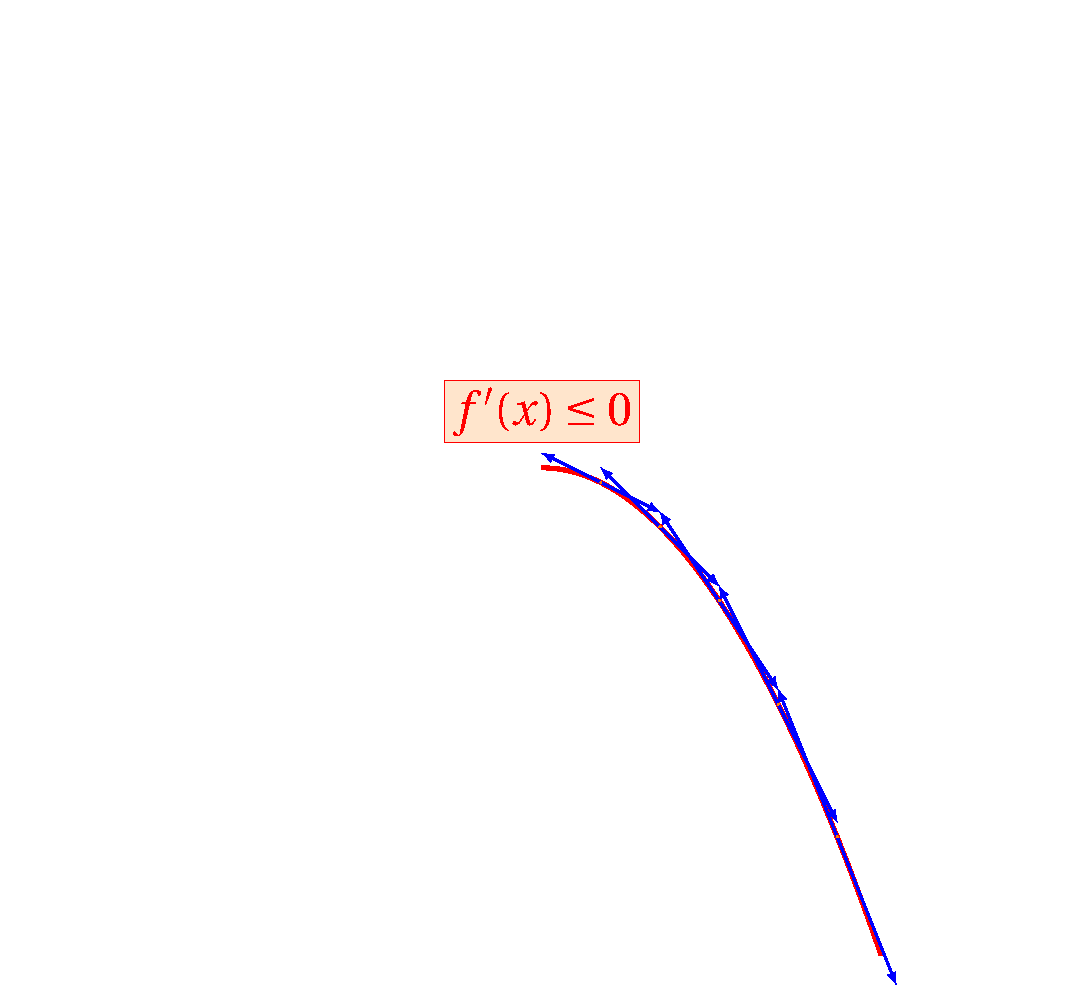
\includegraphics[scale=0.4]{38_home_antalcides_Calculo_pdf_creciente-b.pdf}

\vspace{2pt} Funci�n decreciente%
\end{minipage}\hfill%
\begin{minipage}[c]{0.5\columnwidth}%
\centering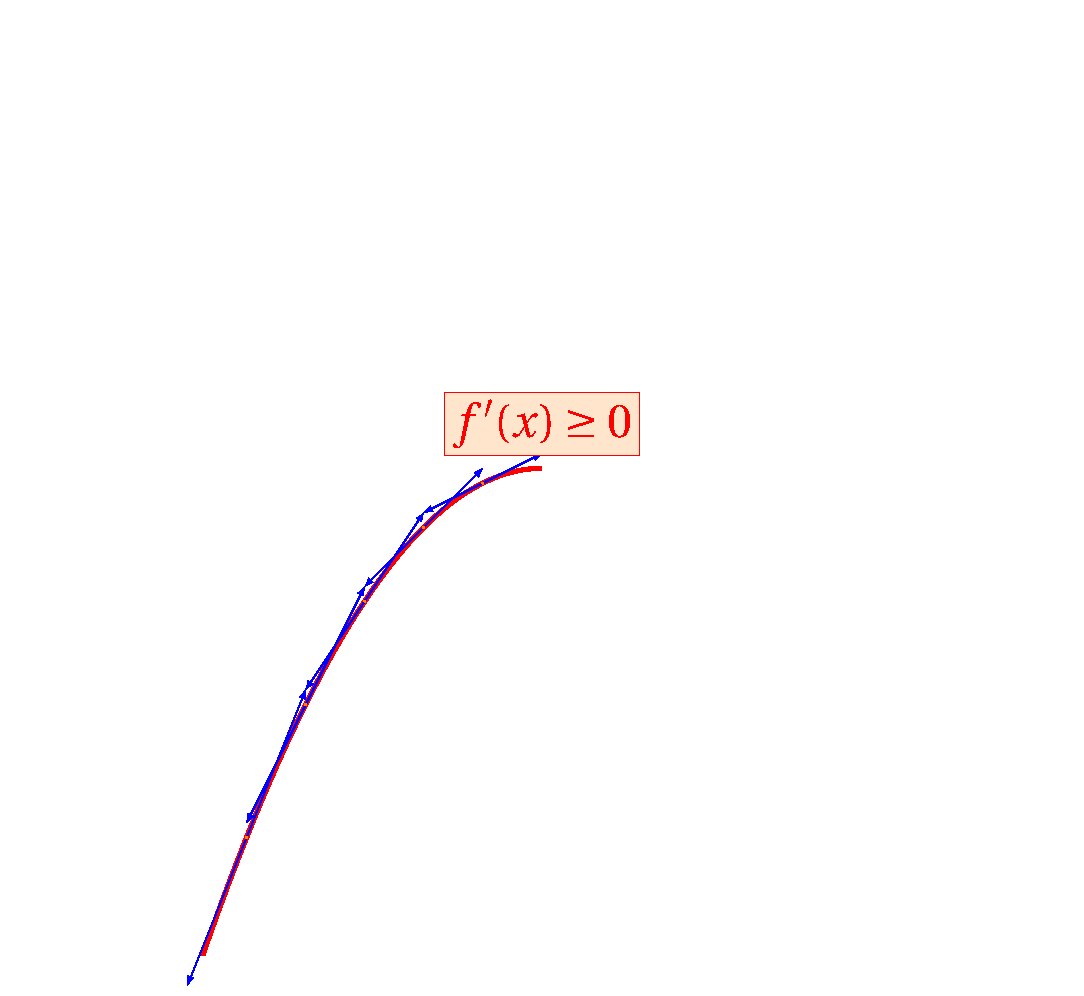
\includegraphics[scale=0.4]{39_home_antalcides_Calculo_pdf_creciente-a.pdf}

\vspace{2pt}Funci�n creciente%
\end{minipage}

Si una funci�n es estrictamente creciente o estrictamente decreciente
se le llama estrictamente mon�tona.

De la proposici�n \eqref{derivmonot} se deduce el siguiente resultado
de extremo absoluto.

\begin{proposicion}{Criterio de extremo absoluto}{extremoabs} Sea
$f$ una funci�n continua en $[a,b]$ y derivable en todo punto de
$]a,b[$ con la posible excepci�n de un punto $c\in]a,b[$. 

{[}a){]} 
\begin{enumerate}
\item Si $f\tl(x)\ge0$ para todo $x\in]a,c[$ y $f\tl(x)\le0$ para todo
$x\in]c,b[$, entonces $f$ alcanza en $c$ un m�ximo absoluto en
$[a,b]$. 
\item Si $f\tl(x)\le0$ para todo $x\in]a,c[$ y $f\tl(x)\ge0$ para todo
$x\in]c,b[$, entonces $f$ alcanza en $c$ un m�nimo absoluto en
$[a,b]$. 
\end{enumerate}
\end{proposicion} \dem \emph{a)} Las hip�tesis hechas implican,
en virtud de la proposici�n \eqref{derivmonot}, que $f$ es creciente
en $[a,c]$ y decreciente en $[c,b]$. Por tanto, se verifica que
$f(x)\le f(c)$ para todo $x\in[a,b]$.

La demostraci�n del apartado \emph{b)} se hace de la misma forma.\fin

El anterior criterio de extremo absoluto suele aplicarse en puntos
donde la derivada se anula. Aunque el resultado anterior est� enunciado
en t�rminos de extremos absolutos, est� claro que si se aplica a un
peque�o intervalo contenido en un intervalo m�s grande, donde la funci�n
est� definida, dicho resultado proporciona en tal caso un criterio
de extremo relativo.

\begin{teo}{}{deriny} Sea $f:I\rightarrow\R$ derivable en el intervalo
$I$ con $f\tl(x)\neq0$ para todo $x\en I$. Se verifica entonces
una de las dos afirmaciones siguientes: 
\begin{itemize}
\item $f$ es estrictamente creciente y $f\tl(x)>0$ para todo $x\en I$. 
\item $f$ es estrictamente decreciente y $f\tl(x)<0$ para todo $x\en I$. 
\end{itemize}
\end{teo} \dem Dados dos puntos $u,v\en I$ con $u\neq v$, podemos
razonar como antes para obtener que existe $c\in]u,v[$ tal que $f(v)-f(u)=f\tl(c)(v-u)\neq0$.
Hemos probado as� que $f$ es inyectiva en el intervalo $I$. Como,
adem�s $f$ es continua en $I$ (por ser derivable), podemos usar
el resultado \ref{continuaeinyectiva} del cap�tulo 4, para deducir
que $f$ es estrictamente mon�tona en $I$. Es suficiente tener en
cuenta ahora la proposici�n anterior para concluir la demostraci�n.\fin

\noindent Es importante advertir que el resultado anterior nos dice
que si una funci�n $f$ es derivable en un intervalo y la derivada
$f\tl$ toma valores positivos y negativos, entonces $f\tl$ se anula
en alg�n punto. Este resultado recuerda mucho al teorema de los ceros
de Bolzano para funciones continuas en un intervalo, con una notable
diferencia: aqu� no exigimos que la funci�n derivada $f\tl$ sea continua.
De hecho, se verifica el siguiente resultado que es un teorema del
valor intermedio para funciones derivadas, en el que no se supone
que la derivada sea continua.

\begin{teo}{Propiedad del valor intermedio para derivadas}{} Sea
$\varphi$ una funci�n definida en un intervalo $I$ que es la derivada
de alguna funci�n en dicho intervalo. Entonces se verifica que la
imagen por $\varphi$ de $I$, $\varphi(I)$, es un intervalo. \end{teo}
\dem Por hip�tesis hay una funci�n derivable \func{f}{I}\ tal
que $\ff(x)=f\tl(x)$ para todo $x\en I$. Sean $u=\ff(a)$, $v=\ff(b)$
dos valores que toma la funci�n \ff, y supongamos $u<v$. Dado $\lambda\in]u,v[$,
definimos la funci�n $g(x)=f(x)-\lambda x$. Tenemos entonces %
\mbox{%
$g\tl(a)=\ff(a)-\lambda=u-\lambda<0$%
} y %
\mbox{%
$g\tl(b)=\ff(b)-\lambda=v-\lambda>0$.%
} Por tanto, la derivada de $g$ toma valores positivos y negativos
en el intervalo $I$ y, por el teorema \ref{deriny}, tiene que anularse,
es decir, existe alg�n punto $c\en I$ tal que $g\tl(c)=\ff(c)-\lambda=0$,
esto es, $\ff(c)=\lambda$. Hemos probado as� que si \ff\ toma dos
valores tambi�n toma todos los comprendidos entre ellos dos, es decir,
que $\ff(I)$ es un intervalo.\fin 

\begin{defi}{Punto cr�tico de primer orden}{pcpo}

Sea $f$ una funci�n definida y derivable en un intervalo $I-\{c\}$
se llama punto cr�tico de primer orden a los puntos de $I$ donde
$f$ est� definida y cumple:
\begin{itemize}
\item Son soluci�n de la ecuaci�n $f'\left(x\right)=0$
\end{itemize}
o
\begin{itemize}
\item Son valores donde $f'\left(x\right)$no est� definida.
\end{itemize}
\end{defi}

\paragraph{Condiciones necesarias de extremo relativo.}

\begin{teo}{Criterio de la primera derivada}{} Sea $c$ un n�mero
cr�tico de una funci�n $f$ continua en un intervalo abierto $I$
que contiene a $c$. Si $f$ es derivable en el intervalo $I$, excepto
a lo sumo en $c$ entonces $f(c)$ puede clasificarse como sigue:
\begin{enumerate}
\item $f\lyxmathsym{\textasciiacute}$ cambia de negativa a positiva en
$c$, $f(c)$ es un m�nimo relativo de $f$. 
\item Si  $f\lyxmathsym{\textasciiacute}$ cambia de positiva a negativa
en $c$, $f(c)$ es un m�ximo relativo de $f$. 3. Si $f\lyxmathsym{\textasciiacute}$
no cambia su signo en $c$, $f(c)$ no es m�nimo ni m�ximo relativo
\end{enumerate}
\end{teo}
\begin{itemize}
\item En las gr�ficas mostraremos las dos condiciones cuando la funci�n
es derivable.
\end{itemize}
\begin{minipage}[t]{0.45\columnwidth}%
\vspace{-10pt}
 \centering 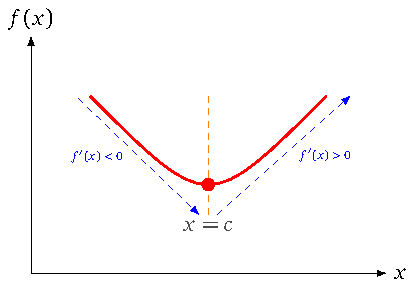
\includegraphics[scale=0.7]{40_home_antalcides_Calculo_pdf_extremos.pdf}
\caption{M�ximo relativo}%
\end{minipage}\hfill%
\begin{minipage}[t]{0.45\columnwidth}%
\vspace{-10pt}
 \centering 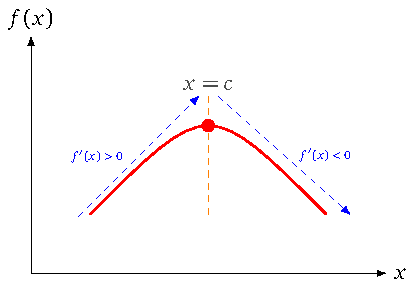
\includegraphics[scale=0.7]{41_home_antalcides_Calculo_pdf_extremos-a.pdf}
\caption{M�nimo relativo}%
\end{minipage}
\begin{itemize}
\item Ahora mostraremos la gr�fica de la segunda condici�n para m�ximos
relativos cuando la funci�n no es derivable.
\end{itemize}
\begin{minipage}[t]{0.9\columnwidth}%
\vspace{-10pt}
 \centering 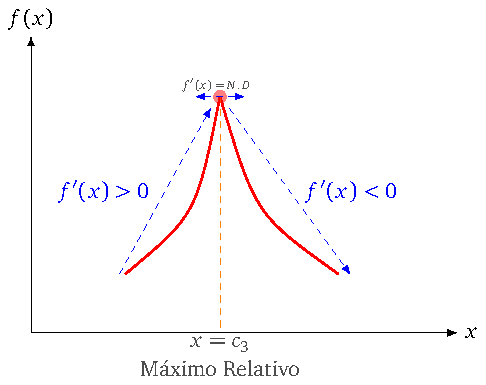
\includegraphics[scale=0.7]{42_home_antalcides_Calculo_pdf_extremos-c.pdf}
\caption{m�ximo  relativo}%
\end{minipage}

Determinar los intervalos donde $f$ es creciente o decreciente es
�til para hallar su gr�fica. Sin embargo, localizando los intervalos
donde $f\lyxmathsym{\textasciiacute}$ crece o decrece, podemos determinar
donde se curva hacia arriba o hacia abajo la gr�fica de $f$ , como
lo estudiaremos a continuaci�n, pero antes mostraremos una gr�fica
para que tengan una idea.

\begin{minipage}[t]{0.9\columnwidth}%
\vspace{-10pt}
 \centering 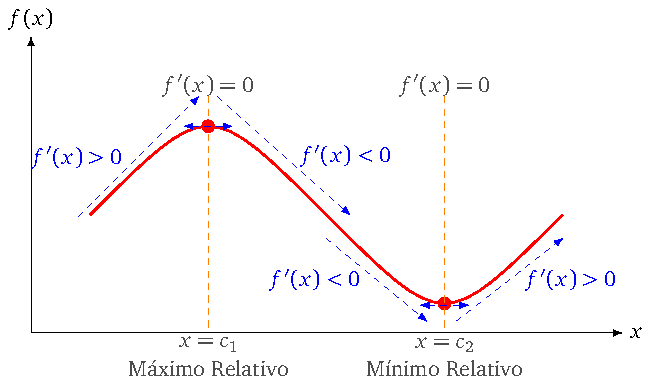
\includegraphics[scale=0.7]{43_home_antalcides_Calculo_pdf_extremos-b.pdf}
\caption{Extremos  relativo}%
\end{minipage}

\begin{teo}{Criterio de la Segunda Derivada}{csd} Sea $f$ una funci�n
tal que $f'(c)=0$ y tal que $f''$ exista en un intervalo abierto
que contenga a $c$. 
\begin{itemize}
\item Si $f''(c)>0$ , entonces $f(c)$ es un m�nimo relativo.
\item Si $f''(c)<0,$ entonces $f(c)$ es un m�ximo relativo.
\item Si  $f''(c)=0,$ entonces el criterio no decide 
\end{itemize}
\end{teo}

\begin{apunte} 

El criterio de la segunda derivadas s�lo puede ser aplicado s�: 
\begin{itemize}
\item $f$ es dos veces derivable en un intervalo abierto que contenga a
$c$ , $f'\left(c\right)=0$ y $f''(c)\neq0.$ 
\item Si el criterio de la segunda derivada no es aplicable, hay que recurrir
a la primera derivada.
\end{itemize}
\end{apunte}

\begin{ejemplo}

\begin{minipage}[t]{0.45\columnwidth}%
\vspace{10pt}

Sea $y=f(x)$ una funci�n cuya derivada tiene una gr�fica como la
que se muestra en la figura.

a) �Qu� se puede decir de $f$ en $x=b$?

b) �Tiene $f$ alg�n m�ximo?

c) �D�nde $f$ decrece?%
\end{minipage}\hfill%
\begin{minipage}[t]{0.45\columnwidth}%
\vspace{10pt}

\centering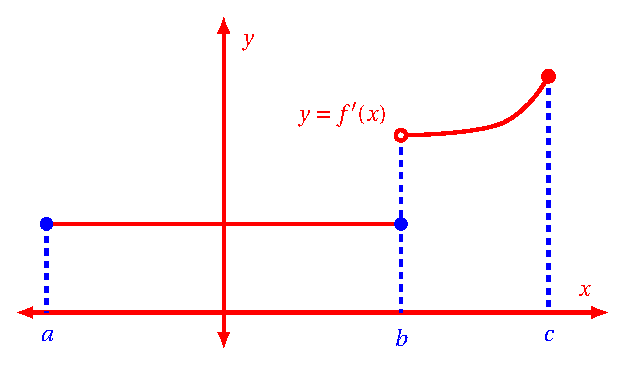
\includegraphics[scale=0.6]{44_home_antalcides_Calculo_pdf_ejsegde.pdf}%
\end{minipage}

\end{ejemplo}

\sol a) De la gr�fica se deduce que $f'(x)$ no es continua en $x=b$,
porque los l�mites laterales son diferentes. Esto indica que la funci�n
$f$ no es derivable en $x=b$. 

b) En todo el intervalo $(a,b)$ la derivada de $f$ es positiva.
Por lo tanto, la funci�n crece.

De la misma manera, en el intervalo $(b,c)$ la funci�n $f$ tambi�n
crece. El m�ximo se encuentra en $c$, que es el extremo derecho del
intervalo donde est� definida la funci�n.

c) De lo anterior se deduce que en ning�n momento la funci�n decrece,
porque la derivada nunca es negativa.\hecho

\begin{ejemplo}

Hallar un polinomio de tercer grado sabiendo que para $x=3$ alcanza
un m�nimo local, para $x=2$ alcanza un m�ximo local y para $x=0$
y $x=1$ toma los valores 1 y 29/6, respectivamente.

\end{ejemplo}

\sol

Escribimos la forma general de un polinomio de grado 3 como $f(x)=ax^{3}+bx^{2}+cx+d$. 

Para $x=0$, $f(0)=1=d$. 

Para $x=1$, $f\left(1\right)=\frac{29}{6}=a+b+c+d$. 

Como $f'(x)=3ax^{2}+2bx+c$, tenemos: 

Para $x=3,\;f'(3)=0=27a+6b+c$. 

Para $x=2$, $f'(2)=0=12a+4b+c$. 

Resulta as� el sistema de ecuaciones: 

\[
\begin{array}{ccc}
a+b+c+d & = & \frac{29}{6}\\
27a+6b+c & = & 0\\
12a+4b+c & = & 0\\
d & = & 1
\end{array}
\]
Al resolver el sistema llegamos a la soluci�n $a=1/3$, $b=-5/2$,
$c=6$, $d=1$, y la funci�n soluci�n es $f(x)=\frac{1}{3}x3-\frac{5}{2}x^{2}+6x+1$.

\hecho

\begin{ejemplo}

Hallar, en caso de que existan, las abscisas de los m�ximos y m�nimos
de la funci�n y
\[
=\frac{1}{3}x^{3}+\frac{5}{2}x^{2}+14x+10\ln(x+3)+90\ln(x-5).
\]

\end{ejemplo}

\sol la primera derivada es:

\[
\begin{aligned}y' & = & x^{2}+5x+14+\frac{10}{x+3}+\frac{90}{x\text{\textminus}5}\\
 &  & \frac{(x^{2}+5x+14)(x+3)(x\text{\textminus}5)+10(x\text{\textminus}5)+90(x+3)}{(x+3)(x\text{\textminus}5)}
\end{aligned}
\]

Al anular la la derivada, obtenemos:

$\begin{array}{ccc}
y'=0 & \Longleftrightarrow & (x^{2}+5x+14)(x+3)(x\text{\textminus}5)+10(x\text{\textminus}5)+90(x+3)=0\\
 & \Longleftrightarrow & x^{4}+3x^{3}\text{\textminus}11x^{2}\text{\textminus}3x+10=0.
\end{array}$

Si aplicamos la regla de Ruffini, resultan las ra�ces $1,$ $-1,$$2$
y $-5.$

Teniendo en cuenta que el dominio de la funci�n es el conjunto $D_{f}=\{x\,|\,x>5\},$
ninguno de los puntos anteriores pertenece al dominio por lo que la
funci�n carece de m�ximos y m�nimos relativos. Adem�s, como $f'\left(x\right)>0,\;\forall\in D_{f}$,
$f$ es siempre creciente. 

\hecho

\begin{ejemplo}

Dada la funci�n $y=(x+1)^{2}e^{-x}$, hallar los m�ximos y m�nimos
locales.

\end{ejemplo}

\sol Calculamos la primera derivada para determinar los puntos cr�ticos:

\[
f'(x)=2(x+1)\text{�}e^{\text{\textminus}x}\text{\textminus}e^{\text{\textminus}x}(x+1)^{2}=e^{\text{\textminus}x}(x+1)(1\text{\textminus}x);
\]

\[
f'(x)=0\Longleftrightarrow e^{\text{\textminus}x}(x+1)(1\text{\textminus}x)=0\Longleftrightarrow x=1\text{\ensuremath{\acute{o}}}x=\text{\textminus}1.
\]

Los �nicos posibles m�ximos y m�nimos se alcanzan en los puntos $P_{1}\left(1,\frac{4}{e}\right)$
y $P_{2}\left(-1,0\right).$

Estudiamos a continuaci�n el crecimiento de la funci�n.
\begin{center}
\begin{tabular}{|c|c|c|c|}
\hline 
 &
$\left(-\infty,-1\right)$ &
$\left(-1,1\right)$ &
$\left(-\infty\right)$\tabularnewline
\hline 
\hline 
$f'\left(x\right)$ &
- &
+ &
-\tabularnewline
\hline 
\end{tabular}
\par\end{center}

De lo anterior se deduce que el punto $P_{1}$es un m�ximo local y
que el punto $P_{2}$ es un m�nimo local de la funci�n \hecho

\begin{teo}{Mon\'otona e inyectiva}{monotonia2}

Sea $f\,:\,\left[a,b\right]\rightarrow\mathbb{R}$ una funci�n estrictamente
mon�tona en $\left[a,b\right]$ entonces $f$ es inyectiva en $\left[a,b\right]$.

\end{teo}

Es decir que si una funci�n es estrictamente mon�tona es invertible.\vspace*{6mm}
 \begin{proposicion}{Derivaci�n de la funci�n inversa}{} Sea $f:I\rightarrow\R$
derivable en el intervalo $I$ con derivada $f\tl(x)\neq0$ para todo
$x\en I$. Entonces $f$ es una biyecci�n de $I$ sobre el intervalo
$J=f(I)$, y la funci�n inversa $f^{-1}:J\rightarrow\R$ es derivable
en $J$ siendo 
\begin{equation}
(f^{-1})\tl(y)=\frac{1}{f\tl(f^{-1}(y))}\qquad(y\in J).\label{derivadainversa}
\end{equation}
\end{proposicion} \dem Las hip�tesis hechas implican que $f$ es
estrictamente mon�tona y continua; por tanto es una biyecci�n de $I$
sobre $J=f(I)$, y la funci�n inversa $f^{-1}:J\rightarrow\R$ es
continua en $J$ (\ref{continuidadinversa}). Sea $b=f(a)\en J$.
Puesto que 
\[
\Lim{\frac{x-a}{f(x)-f(a)}}{x}{a}=\frac{1}{f\tl(a)},
\]
la funci�n \func{h}{I}\ dada por: 
\[
h(x)=\frac{x-a}{f(x)-f(a)}\quad\textrm{para }\ x\neq a,\quad h(a)=\frac{1}{f\tl(a)}
\]
es continua en $I$. Como $f^{-1}$ es continua en $J$, deducimos
que $h\circ f^{-1}$ es continua en $J$, por lo que, en particular,
$\Lim{h(f^{-1}(y))}{y}{b}=h(f^{-1}(b))=h(a)$. Pero, para todo $y\en J$,
con $y\neq b$ es 
\[
h(f^{-1}(y))=\frac{f^{-1}(y)-f^{-1}(b)}{y-b}.
\]
Concluimos as� que 
\[
\Lim{\frac{f^{-1}(y)-f^{-1}(b)}{y-b}}{y}{b}=\frac{1}{f\tl(a)}
\]
\fin La mejor forma de recordar la igualdad \eqref{derivadainversa}
es derivar por la regla de la cadena la identidad $(f\circ f^{-1})(y)=y$,
con lo que se obtiene $f\tl(f^{-1}(y))(f^{-1})\tl(y)=1$, de donde
puede despejarse $(f^{-1})\tl(y)$.

\subsection{Funciones trigonom�tricas inversas}

\paragraph{\noindent Derivabilidad de las funciones trigonom�tricas inversas}

\noindent \begin{ejemplo} La funci�n tangente es una biyecci�n derivable
del intervalo $]-\pi/2,\pi/2[$ sobre \R, cuya derivada no se anula.
El teorema anterior nos dice que la funci�n inversa, es decir, la
funci�n arcotangente es derivable en \R\ y su derivada podemos calcularla
derivando la identidad $(\tg\circ\arctg)(x)=x$, con lo que obtenemos
\[
(1+\tg^{2}(\arctg x))\arctg\tl(x)=1\ms{3mu}\Longleftrightarrow\ms{3mu}(1+x^{2})\arctg\tl(x)=1\ms{3mu}\Longleftrightarrow\ms{3mu}\arctg\tl(x)=\frac{1}{1+x^{2}}
\]
An�logamente, la funci�n seno es una biyecci�n derivable del intervalo
$]-\pi/2,\pi/2[$ sobre $]-1,1[$ cuya derivada no se anula. El teorema
anterior nos dice que la funci�n inversa, es decir, la funci�n arcoseno
es derivable en $]-1,1[$ y su derivada podemos calcularla derivando
la identidad $(\sen\circ\arcsen)(x)=x$, con lo que obtenemos: 
\[
\cos(\arcsen x)\arcsen\tl(x)=1\ms{3mu}\Longleftrightarrow\ms{3mu}\sqrt{1-x^{2}}\arcsen\tl(x)=1\ms{3mu}\Longleftrightarrow\ms{3mu}\arcsen\tl(x)=\frac{1}{\sqrt{1-x^{2}}}
\]
\end{ejemplo}

\subsubsection{Funci�n Arco-seno}

\subsubsection{Funci�n Arco-coseno}

\subsubsection{Funci�n Arco-tangente}

\subsubsection{Funci�n Arco-cotangente}

\subsubsection{Funci�n Arco-secante}

\subsubsection{Funci�n Arco-cosecante}

\subsection{Concavidad}

\subsubsection{Puntos cr�ticos de segundo orden}

\begin{defi}{Punto cr�tico de segundo orden}{pcso}

Sea $f$ una funci�n definida y que admite segunda derivada en un
intervalo $I-\{c\}$ se llama punto cr�tico de segundo orden a los
puntos de $I$ donde $f$ est� definida y cumple:
\begin{itemize}
\item Son soluci�n de la ecuaci�n $f''\left(x\right)=0$
\end{itemize}
o
\begin{itemize}
\item Son valores donde $f''\left(x\right)$no est� definida.
\end{itemize}
\end{defi}

\section{Funciones convexas y funciones c�ncavas}

\begin{defi}{}{} Dados dos puntos $\boldmath{\alpha}=(a,b)$ y $\boldmath{\beta}=(c,d)$
en el plano, el segmento que une $\boldmath{\alpha}$ con $\boldmath{\beta}$
es el conjunto de puntos del plano: 
\begin{equation}
[\boldmath{\alpha},\boldmath{\beta}]=\set{t\boldmath{\alpha}+(1-t)\boldmath{\beta}:0\le t\le1}=\set{\big(ta+(1-t)c,tb+(1-t)d\big):0\le t\le1}\label{segmento}
\end{equation}
\end{defi} Observa que si $x<y$ son n�meros reales, el segmento
que une $x$ con $y$ es el intervalo cerrado $[x,y]$.

\begin{defi}{Concavidad}{} Sea \func{f}{I}\ una funci�n definida
en un intervalo $I$. Se dice que $f$ es \emph{convexa} en $I$ si
para todo par de puntos $x,y\en I$ y para todo $t$ con $0\le t\le1$,
se verifica que: 
\begin{equation}
f(tx+(1-t)y)\le tf(x)+(1-t)f(y)\label{convexidad}
\end{equation}
Cuando la desigualdad anterior es estricta para $0<t<1$ se dice que
$f$ es \emph{estrictamente convexa}. Se dice que $f$ es \emph{c�ncava}
en $I$ cuando $-f$ es convexa en $I$ y \emph{estrictamente c�ncava}
cuando $-f$ es estrictamente convexa. \end{defi}

La interpretaci�n geom�trica de esta desigualdad es la siguiente.
El segmento que une el punto del plano $(x,f(x))$ con el punto $(y,f(y))$
es el conjunto 
\[
\set{\big(tx+(1-t)y,tf(x)+(1-t)f(y)\big):0\le t\le1}
\]
La desigualdad \eqref{convexidad} dice que la ordenada, $tf(x)+(1-t)f(y)$,
de cada punto de dicho segmento es mayor o igual que el valor de $f$
en la abscisa $f(tx+(1-t)y)$. Es decir, el punto $\big(tx+(1-t)y,tf(x)+(1-t)f(y)\big)$
queda por encima del punto $\big(tx+(1-t)y,f(tx+(1-t)y)\big)$. Dicho
de otra forma: el segmento (la cuerda) que une dos puntos de la gr�fica
de $f$ queda siempre por encima de la gr�fica de $f$.

\begin{figure}[ht]
\begin{minipage}[t]{0.45\textwidth}%
\vspace{0pt}
 \centering %singlelinecheck=off,
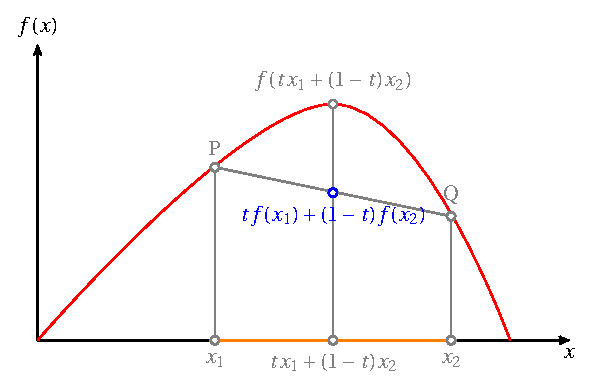
\includegraphics[scale=0.5]{45_home_antalcides_Calculo_pdf_concavidad-abj.pdf}\caption{Funci�n c�ncava}
\label{fig:concava} %
\end{minipage}%
\begin{minipage}[t]{0.45\textwidth}%
\vspace{0pt}
 \centering 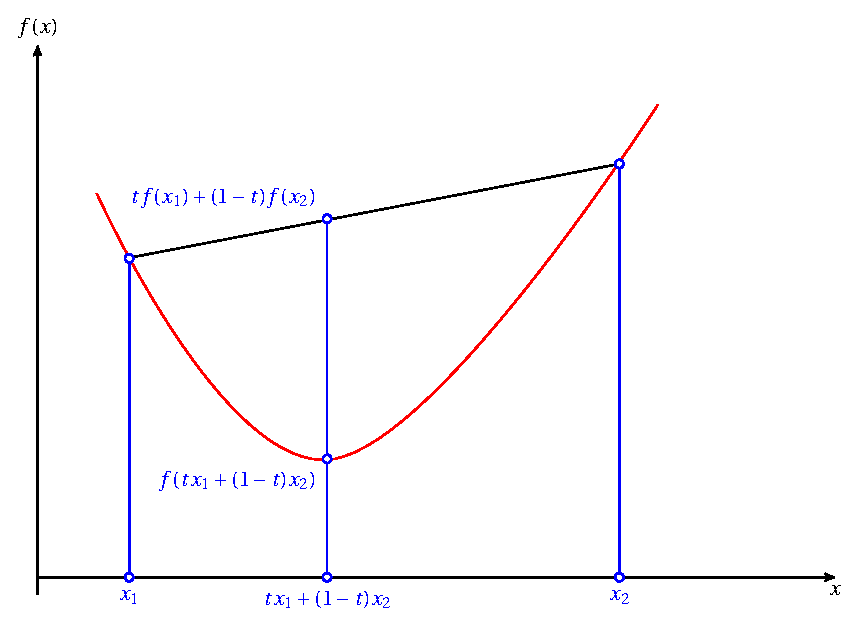
\includegraphics[scale=0.4]{46_home_antalcides_Calculo_pdf_concavidad-arr.pdf}\captionsetup{,margin=1cm}
\caption{Funci�n convexa}
\label{fig:convexa} %
\end{minipage}
\end{figure}

Naturalmente, para una funci�n c�ncava se verifica la desigualdad
opuesta a \eqref{convexidad} y, por tanto, si $f$ es c�ncava el
segmento (la cuerda) que une dos puntos de la gr�fica de $f$ queda
siempre por debajo de la gr�fica de $f$.

Las gr�ficas \eqref{fig:convexa} y \eqref{fig:concava} muestran
claramente estos comportamientos.

Es decir desde el punto de vista geom�trico Una funci�n se dice c�ncava
hacia arriba o convexa en un intervalo $(a,b)$ cuando al unir dos
puntos de la curva en ese intervalo, el segmento que se forma queda
por encima de la curva. De la misma forma, ser� c�ncava hacia abajo
o c�ncava cuando cualquiera de dichos segmentos queda por debajo de
la curva. Ilustramos estos casos con las siguientes gr�ficas.

\begin{minipage}[t]{0.45\textwidth}%
\vspace{0pt}
 \centering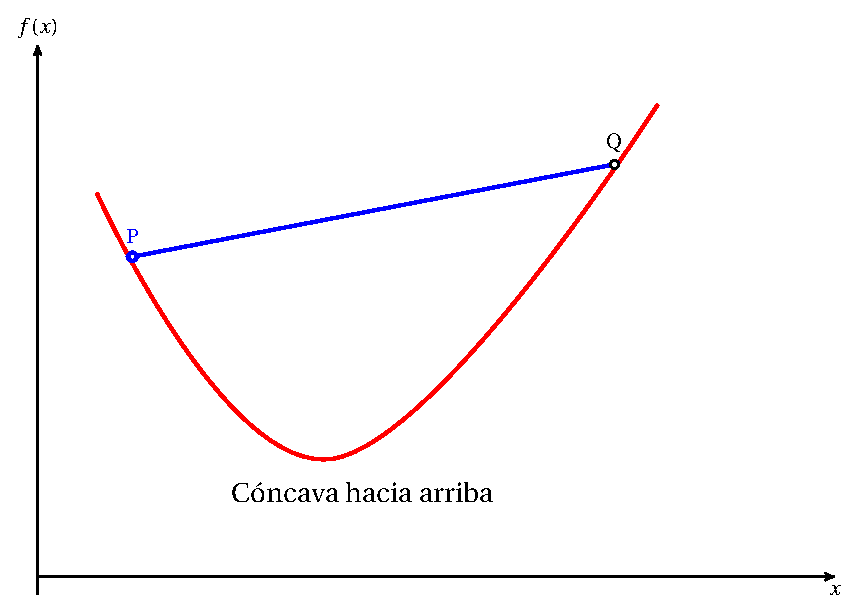
\includegraphics[scale=0.5]{47_home_antalcides_Calculo_pdf_concavidad-c.pdf}\label{fig:concava-3-1} %
\end{minipage}%
\begin{minipage}[t]{0.45\textwidth}%
\vspace{10pt}
 \centering 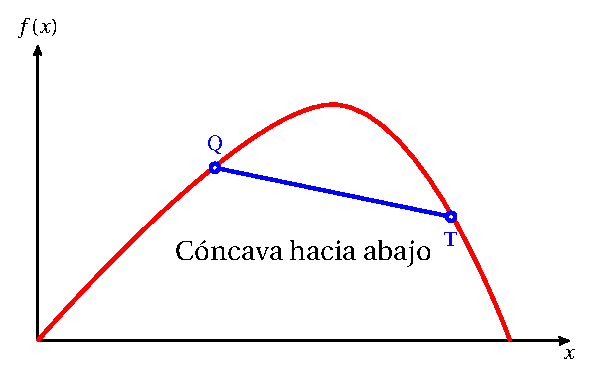
\includegraphics[scale=0.8]{48_home_antalcides_Calculo_pdf_concavidad-d.pdf}\label{fig:convexa-2-1} %
\end{minipage}

En este caso se puede trazar por lo menos un segmento donde la curva
no esta totalment or encima o por debajo de ella.

\begin{minipage}[t]{0.9\textwidth}%
\vspace{0pt}
 \centering 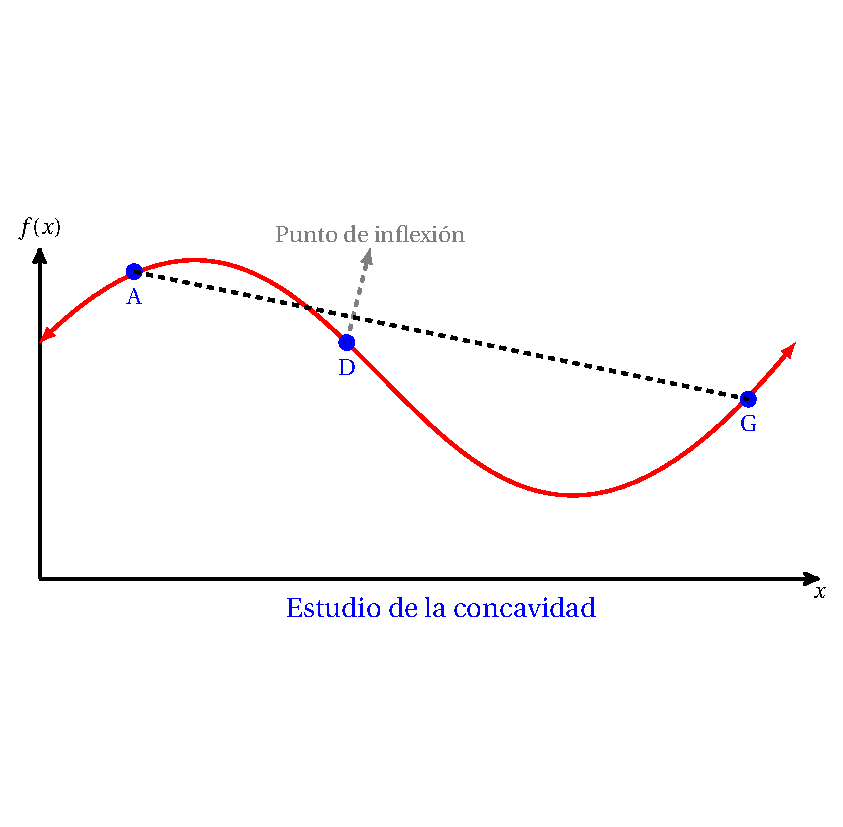
\includegraphics[scale=0.6]{49_home_antalcides_Calculo_pdf_est-concavidad.pdf}
\label{fig:convexa-2-2} %
\end{minipage}

Ejemplos t�picos de funciones convexas son las par�bolas ``hacia
arriba'' y la exponencial. Ejemplos t�picos de funciones c�ncavas
son las par�bolas ``hacia abajo'' y el logaritmo.

Para funciones derivables se tiene una �til caracterizaci�n de la
convexidad.

\begin{teo}{Condiciones suficientes de convexidad}{} Supongamos que
$f$ es continua en $[a,b]$ y derivable en $]a,b[$. Si la derivada
de $f$ es creciente (resp. estrictamente creciente) en $]a,b[$ entonces
$f$ es convexa (resp. estrictamente convexa) en $[a,b]$. En particular
si $f$ es dos veces derivable en $]a,b[$ y se verifica que $f\scd(x)\ge0$
(resp. $f\scd(x)\leq0$) para todo $x\in]a,b[$, entonces $f$ es
convexa (resp. estrictamente convexa) en $[a,b]$. \end{teo} \dem
Sean $x,y\in[a,b]$ con $x<y$. Sea $t\in]0,1[$ y pongamos $z=tx+(1-t)y$.
Hay que probar que $f(z)\le tf(x)+(1-t)f(y)$. Puesto que $f(z)=tf(z)+(1-t)f(z)$,
esta desigualdad puede escribirse 
\[
tf(z)+(1-t)f(z)\le tf(x)+(1-t)f(y)\quad\Longleftrightarrow\quad(1-t)\big(f(z)-f(x)\big)\le t\big(f(y)-f(z)\big)
\]
Aplicando el TVM en los intervalos $[x,z]$ y $[z,y]$, obtenemos
puntos $c\in]x,z[$, $d\in]z,y[$ tales que 
\[
f(z)-f(x)=f\tl(c)(z-x),\qquad f(y)-f(z)=f\tl(d)(y-z)
\]
Teniendo en cuenta que $f\tl$ se supone creciente, por lo que $f\tl(c)\le f\tl(d)$,
y la igualdad de comprobaci�n inmediata $(1-t)(z-x)=t(y-z)$, se tiene
que: 
\[
(1-t)\big(f(z)-f(x)\big)=(1-t)f\tl(c)(z-x)\le tf\tl(d)(y-z)=t\big(f(y)-f(z)\big)
\]
Que es la desigualdad que quer�amos probar.\fin

Interpretando la derivada primera como la velocidad y la derivada
segunda como la aceleraci�n, las curvas convexas aceleran y las c�ncavas
frenan.

Observa que si $f$ es una funci�n convexa y derivable en un intervalo
$I$, entonces la gr�fica de $f$ queda siempre por encima de la recta
tangente en cualquier punto, es decir, para todo par de puntos $x,a\en I$
se verifica que %
\mbox{%
$f(x)\geqslant f(a)+f\tl(a)(x-a)$%
}. De hecho, para funciones derivables, esta propiedad es equivalente
a la convexidad (ver ejercicio \ref{ejer:convex}).

\begin{defi}{Punto de inflexi�n}{} Se dice que $a\in D_{f}$ es un
\textbf{punto de inflexi�n} de una funci�n $f$, si hay un n�mero
$r>0$ tal que $f$ es c�ncava en el intervalo $]a-r,a[$ y $f$ es
convexa en el intervalo $]a,a+r[$ (o al rev�s). Es decir, los puntos
en los que una funci�n pasa de c�ncava a convexa o de convexa a c�ncava
se llaman puntos de inflexi�n. \end{defi}

El siguiente resultado se prueba f�cilmente y queda como ejercicio.

\begin{proposicion}{}{} Si $f$ tiene un punto de inflexi�n en $a\in I$
y es dos veces derivable en $I$ excepto quiz�s en $x=a$, entonces
$f\scd(a)=0$ o $f\scd(a)$ no est� definida .

Si $f$ es tres veces derivable en un punto $a$ y se tiene que $f\scd(a)=0$
pero $f^{\prime\mspace{-2mu}\prime\mspace{-2mu}\prime}(a)\neq0$,
entonces $f$ tiene un punto de inflexi�n en $a$. \end{proposicion}

\begin{minipage}[t]{0.45\textwidth}%
\vspace{0pt}
 \centering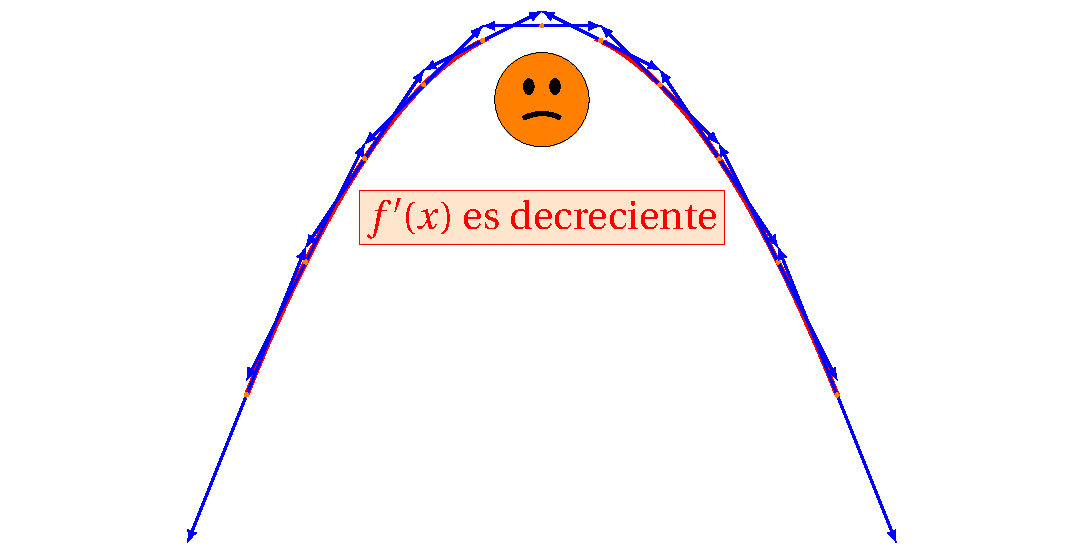
\includegraphics[scale=0.4]{50_home_antalcides_Calculo_pdf_concavidad-b.pdf}%
\end{minipage}%
\begin{minipage}[t]{0.45\textwidth}%
\vspace{10pt}
 \centering 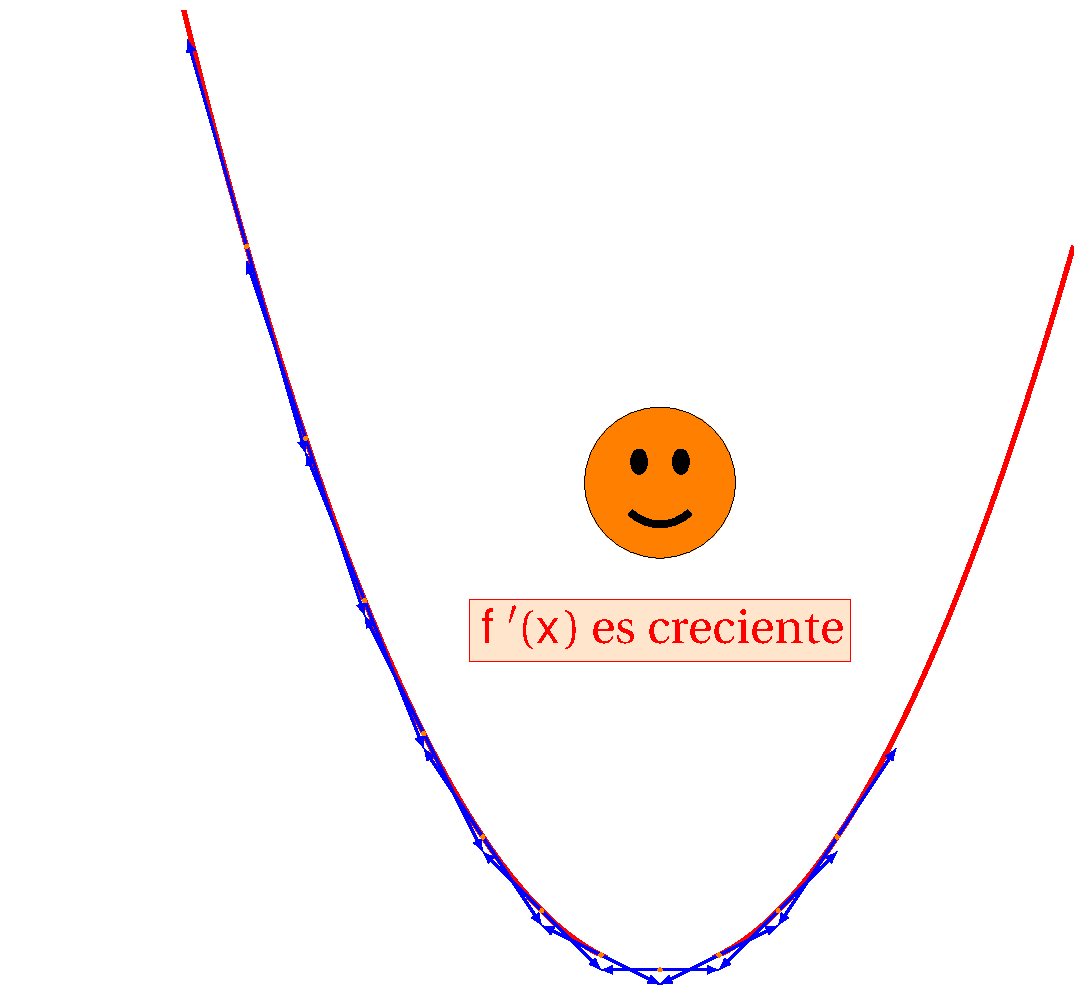
\includegraphics[scale=0.3]{51_home_antalcides_Calculo_pdf_concavidad-a.pdf}%
\end{minipage}

De la figura anterior, se puede deducir la siguiente interpretaci�n
gr�fica de la concavidad. 
\begin{itemize}
\item Si una curva est� por encima de sus rectas tangentes, es c�ncava hacia
arriba.
\item Si una curva est� por debajo de las rectas tangentes es c�ncava hacia
abajo.
\end{itemize}
Para determinar la concavidad sin ver la gr�fica de $f$, podemos
usar la segunda derivada para distinguir donde crece o decrece $f'$.
Bastar� con tener en mente que la segunda derivada de $f$ es la primera
de $f'$. Por lo tanto, $f'$ es creciente si $f''$ es positiva y
decreciente si $f''$ es negativa. 

\begin{apunte}Si la gr�fica de una funci�n continua posee recta tangente
en un punto donde la concavidad cambia de sentido, llamamos a ese
punto de inflexi�n.\end{apunte}

\begin{ejemplo}

Estudiar la concavidad de la funci�n $f(x)=\frac{x^{2}}{1+x}$ y localizar
sus puntos de inflexi�n.

\end{ejemplo}

\sol En primer lugar calcularemos las derivadas de primer y segundo
orden de la funci�n: 
\[
f'(x)=\frac{2x(1+x)-x^{2}}{(1+x)^{2}}=\frac{x^{2}+2x}{\left(1+x\right)^{2}}.
\]

\[
\begin{array}{ccc}
f''\left(x\right) & = & \frac{(2x+2)(1+x)^{2}\text{\textminus}(x^{2}+2x)\text{�}2(1+x)}{(1+x)4}\\
 & = & \frac{(2x+2)(1+x)\text{\textminus}(x^{2}+2x)\text{�}2}{(1+x)^{3}}=\frac{2}{(1+x)^{3}}.
\end{array}
\]
Para estudiar el signo de la segunda derivada, observamos que el numerador
nunca se anula.

En cambio, el denominador se anula en el punto de abscisa $x=-1$,
que es precisamente el punto que no est� en el dominio. 

Para estudiar el signo en los intervalos que este punto determina,
construimos el siguiente diagrama de signos:
\begin{center}
\begin{tabular}{|c|c|c|}
\hline 
 &
$\left(-\infty,-1\right)$ &
$\left(-1,\infty\right)$\tabularnewline
\hline 
\hline 
$f''\left(x\right)$ &
- &
+\tabularnewline
\hline 
\end{tabular}
\par\end{center}

Al calcular $f''(x)$ en un punto del intervalo $(-\infty,-1)$ result�
un valor negativo y al sustituir en la funci�n un punto del intervalo
$(-1,\infty)$ el fue positivo. Eso quiere decir que: $f$ es c�ncava
hacia arriba en el intervalo $(-1,\infty)$; $f$ es c�ncava hacia
abajo en el intervalo $(-\infty,-1)$. Sin embargo no hay punto de
inflexi�n pues el punto $x=-1$, en donde cambia la concavidad, no
est� en el dominio\hecho

\section{Graficaci�n}

En este apartado se resumen todas las t�cnicas estudiadas anteriormente
y se agrupan para dibujar con relativa precisi�n las curvas correspondientes
a funciones definidas en forma expl�cita. Toda la informaci�n que
se pueda obtener de la funci�n ser� �til para conseguir una gr�fica
m�s exacta. En la primera parte se dar�n algunas informaciones de
cierta funci�n desconocida y se tratar� de dibujar una funci�n que
verifique dichos datos. El m�todo m�s adecuado consiste en seguir
los siguientes pasos: 
\begin{enumerate}
\item Determine el dominio de la funci�n.
\item Determine los puntos de corte con los ejes coordenados , $x=0$, $f\left(x\right)=0.$
\item estudiar la simetr�a de la gr�fica.
\item Estudiar la continuidad de la funci�n.
\item Determinar las as�ntotas si las hay.
\item Construir una tabla donde se expresen los intervalos conocidos de
crecimiento y concavidad de la funci�n, tal como se hizo en los apartados
anteriores.
\item Dibujar en un sistema de coordenadas los puntos por donde se sepa
que pasa la funci�n, es decir si encontramos  m�ximos, m�nimos , puntos
de inflexi�n y puntos de corte con los ejes. Despu�s se deben trazar
las as�ntotas conocidas.
\item Por �ltimo, trazar \textquotedblright pedazos\textquotedblright de
curva que tengan la forma indicada por el crecimiento y la concavidad
correspondientes a cada intervalo, y de acuerdo a la tabla construida,
de modo que pase por los puntos dibujados en el paso anterior y tenga
como as�ntotas las ya dibujadas.
\end{enumerate}
\begin{ejemplo}\\
Estudie el comportamiento de la gr�fica de la funci�n 
\[
f\left(x\right)=2x^{2}-x^{4}
\]

\end{ejemplo}

\sol Realizaremos todos los pasos para trazar la gr�fica de $f.$
\begin{itemize}
\item Como $f$ es un polinomio entonces su dominio de $\R$.
\item La funci�n es par $f\left(x\right)=f\left(-x\right)=2\left(-x\right)^{2}-\left(-x\right)^{4}=2x^{2}-x^{4},$
la gr�fica de $f$ tiene el eje $OY$ por eje de simetr�a� (simetr�a
axial), es decir es sim�trica con respecto al eje $y$. Como el punto
$(x-y)$ no pertenece a la gr�fica entonces la funci�n no es sim�trica
con respecto al eje $x$, y como el punto $(-x,-y)$ no pertenece
a la gr�fica no es sim�trica con respecto al origen. 
\item Calcularemos los puntos de intersecci�n con los ejes es decir los
puntos donde $y=0$ y $x=0$
\[
f\left(x\right)=x^{2}\left(2-x^{2}\right)=0.
\]
Por tanto las soluciones son $x=0$ y $x=\pm\sqrt{2}\Rightarrow y=0$
, en los tres casos.
\[
x=0\Rightarrow f\left(0\right)=0\Rightarrow y=0.
\]
Es decir los puntos son de intersecci�n con los ejes son, $(0,0),$
($\sqrt{2},0)$ y $(-\sqrt{2},0)$. 
\item Como la funci�n es polin�mica entonces es continua en $\R.$
\item No tiene as�ntotas.
\item Calcularemos las dos primeras derivadas,
\[
f'\left(x\right)=4x-4x^{3}
\]
\[
f''\left(x\right)=4-12x.
\]
Primero analizaremos la primera derivada y para ello calculamos los
valores cr�ticos de las inecuaciones 
\[
4x-4x^{3}<0\vee4x-4x^{3}>0,
\]
los cuales son $x=-1,x=1,x=0$ de aqu� se obtienen los intervalos
donde la derivada cambia de signo es decir en $(-\infty,-1),\:(0,1),\:\left(-1,0\right)$y
$\left(1,+\infty\right)$, entonces tomamos un valores de prueba para
cada uno de los intervalos como por ejemplo. $-1.1\:,-0.99,\:0.1,\:1.1$
y evaluamos la derivada en cada punto. De lo anterior se deduce que
la derivada es positiva en $(-\infty,-1),(0,1)$ y es negativa en
$\left(-1,0\right),\left(1,+\infty\right)$, colocamos los resultados
en una tabla.\vspace{10pt}
Realizamos el mismo procedimiento para la segunda derivada $f''\left(x\right)$
obteniendo que la segunda derivada es negativa en $\left(-\infty,{\displaystyle \frac{-1}{\sqrt{3}}}\right)$,$\left({\displaystyle \frac{{\displaystyle 1}}{\sqrt{3}}},+\infty\right)$
y es positiva en $\left({\displaystyle \frac{-1}{{\displaystyle \sqrt{3}}}},{\displaystyle {\displaystyle {\displaystyle \frac{1}{{\displaystyle \sqrt{3}}}}}}\right)$ 
\end{itemize}
Podemos resumir toda la informaci�n en una tabla.\vspace*{30pt}

\begin{tabular}{|c|c|c|c|c|c|c|c|c|c|c|c|c|}
\hline 
$-\infty$  &
\textbf{\footnotesize{}Forma}{\footnotesize{} } &
\textbf{\footnotesize{}$-1$}{\footnotesize{} } &
\textbf{\footnotesize{}Forma}{\footnotesize{} } &
\textbf{\footnotesize{}$\frac{-1}{\sqrt{3}}$}{\footnotesize{} } &
\textbf{\footnotesize{}Forma}{\footnotesize{} } &
\textbf{\footnotesize{}$0$}{\footnotesize{} } &
\textbf{\footnotesize{}Forma}{\footnotesize{} } &
\textbf{\footnotesize{}$\frac{1}{\sqrt{3}}$}{\footnotesize{} } &
\textbf{\footnotesize{}Forma}{\footnotesize{} } &
\textbf{\footnotesize{}$1$}{\footnotesize{} } &
\textbf{\footnotesize{}Forma}{\footnotesize{} } &
$\infty$\tabularnewline
\hline 
\hline 
 &
\multirow{2}{*}{$\nearrow$$\curvearrowright$}  &
\multirow{2}{*}{ Max}  &
\multirow{2}{*}{$\searrow$$\curvearrowright$}  &
\multirow{2}{*}{P.I}  &
\multirow{2}{*}{$\searrow$\ro}  &
\multirow{2}{*}{Min}  &
\multirow{2}{*}{$\nearrow$\ro}  &
\multirow{2}{*}{P.I}  &
\multirow{2}{*}{$\nearrow$$\curvearrowright$}  &
\multirow{2}{*}{Max}  &
\multirow{2}{*}{$\searrow$$\curvearrowright$}  &
\multirow{2}{*}{}\tabularnewline
 &
 &
 &
 &
 &
 &
 &
 &
 &
 &
 &
 &
\tabularnewline
\hline 
\end{tabular}
\begin{figure}[H]
\centering

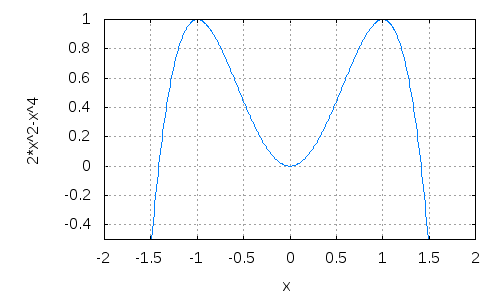
\includegraphics[scale=0.5,bb = 0 0 200 100, draft, type=eps]{/media/antalcides/Antalcides-EXT/maletin/ua12016/asignaturas/talleres/lyx_mathway/figuras/6_media_ANTALCIDES____talleresmat_optimizacion.png}\caption{Graficaci�n}

\label{fig3} 
\end{figure}

Al observar la gr�fica(\ref{fig3}) podemos concluir que : 
\begin{itemize}
\item Es sim�trica con respecto al eje $y$. 
\item Tiene m�ximos relativos en $x=-1,x=1$ y esta de acuerdo con el resumen
de la tabla donde la gr�fica cambia de creciente a decreciente. 
\item Tiene un m�nimo relativo en $x=0$ como se deduce en la tabla que
cambia de decreciente a decreciente. 
\item Hay puntos de inflexi�n en $x=-\frac{{\displaystyle 1}}{\sqrt{3}},\:x=\frac{{\displaystyle 1}}{\sqrt{3}}$
es decir la concavidad en esos puntos. 
\item En $\left(-\infty,{\displaystyle \frac{-1}{\sqrt{3}}}\right)$,$\left({\displaystyle \frac{{\displaystyle 1}}{\sqrt{3}}},+\infty\right)$
es c�ncava hacia abajo y en $\left({\displaystyle \frac{-1}{{\displaystyle \sqrt{3}}}},{\displaystyle {\displaystyle {\displaystyle \frac{1}{{\displaystyle \sqrt{3}}}}}}\right)$
es c�ncava hacia arriba.
\end{itemize}
\hecho

\begin{ejemplo} Dada la funci�n
\[
f(x)=\frac{\sqrt{x}}{1+x^{2}}
\]

\begin{description}
\item [{(a)}] Estudiar su dominio, puntos de corte y as�ntotas. 
\item [{(b)}] Calcular su funci�n derivada primera. �Est� dicha funci�n
definida en $x=0$? Hallar la derivada en el punto $x=1$. 
\item [{(c)}] Determinar sus intervalos de crecimiento y decrecimiento,
as� como sus m�ximos y m�nimos relativos. 
\item [{(d)}] Representar su gr�fica. 
\end{description}
\end{ejemplo} 

\sol\textbf{(a)} Al estudiar el dominio, la ra�z cuadrada nos indica
que $x\ge0$. Pero tambi�n deber�amos plantearnos si es posible que
el denominador sea cero. Por supuesto, esto es imposible, pues $1+x^{2}$
siempre toma valores estrictamente positivos. 

Continuando con el problema, vamos a estudiar los puntos de corte. 

A continuaci�n, podemos estudiar el punto de corte con el eje de ordenadas,
obteniendo el punto $(0,0)$: la funci�n no tiene asintotas (�Porqu�?).

\textbf{(b)} Calculamos ahora las dos primeras derivadas

En el cociente $f'\left(x\right)=-\frac{(3x^{2}-1)}{(2\sqrt{x}(x^{2}+1)^{2})}$
se aprecia perfectamente que la funci�n no est� definida en $x=0$,
pues en tal caso estar�amos dividiendo por cero. Esto se ve con claridad
si sustituimos $x=0$ y se anula en $x=\pm\frac{\sqrt{3}}{3}.$

La segunda derivada nos da \[f''(x)=-\frac{1-3\cdot {{x}^{2}}}{4\cdot {{x}^{\frac{3}{2}}}\cdot {{\left( 1+{{x}^{2}}\right) }^{2}}}-\frac{3\cdot \sqrt{x}}{{{\left( 1+{{x}^{2}}\right) }^{2}}}-\frac{2\cdot \sqrt{x}\cdot \left( 1-3\cdot {{x}^{2}}\right) }{{{\left( 1+{{x}^{2}}\right) }^{3}}}\]

\textbf{(c)} Para estudiar el crecimiento y extremos relativos de
$f(x)$ estudiaremos sus puntos cr�ticos. 

As�, $f'(x)>0$ en $(0,1/\sqrt{3})$ ($f$ creciente) y $f'(x)<0$
en $(1/\sqrt{3},+\infty)$ ($f$ decreciente). Por supuesto, tenemos
un m�ximo relativo (y, en este caso, absoluto) en $x=1/3$.

\textbf{(d)} 

\begin{figure}[H]
\centering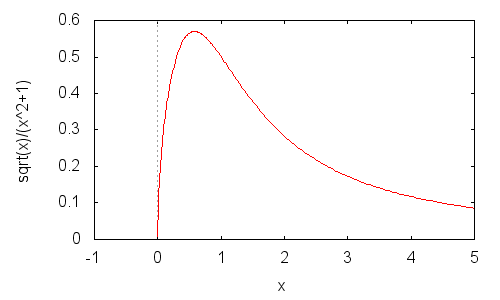
\includegraphics[scale=0.6,bb = 0 0 200 100, draft, type=eps]{/media/antalcides/Antalcides-EXT/maletin/ua12016/asignaturas/talleres/lyx_mathway/figuras/7_media_ANTALCIDES____talleresmat_ej6.png}

\caption{Trazado de una gr�fica}

\label{fig6} 
\end{figure}

\hecho

\begin{ejemplo} Estudie el comportamiento de la gr�fica de la funci�n
\[
f(x)=\frac{4x}{x^{2}-1}.
\]

\end{ejemplo}

\sol
\begin{itemize}
\item Calculemos los puntos de intersecci�n con los ejes 
\end{itemize}
La gr�fica interseca a los ejes en el punto $(0,0).$ 
\begin{itemize}
\item Determinemos las as�ntotas 
\end{itemize}
Para determinar las as�ntotas debemos encontrar los valores para los
cuales el denominador es cero y 
\[
\lim_{x\rightarrow-\infty}f(x)\:\mbox{y \ensuremath{\lim_{x\rightarrow+\infty}f(x).}}
\]

Hay as�ntotas verticales en $x=-1$ y $x=1,$ adem�s el eje $x$ es
una as�ntota horizontal. 
\begin{itemize}
\item Puntos cr�ticos. 
\end{itemize}
Calcularemos la primera derivada y la igualamos a $0$ para determinar
los puntos cr�ticos.

Como la soluci�n no est� en el conjunto $\mathbb{R}$, entonces no
hay puntos cr�ticos, por tanto la funci�n no tiene extremos relativos. 
\begin{itemize}
\item Monoton�a 
\end{itemize}
Como la funci�n no tiene extremos relativos debe ser mon�tona, veamos
si es creciente o decreciente.

Como la derivada no es positiva entonces la funci�n es decreciente. 
\begin{itemize}
\item Puntos de inflexi�n y concavidad. 
\end{itemize}
Debemos ahora calcular la segunda derivada y analizar su signo.

De acuerdo con el resultado hay un punto de inflexi�n en $x=0.$

Ahora analicemos el signo entre $\left(-\infty,-1\right),\:\left(-1,0\right),\:\left(0,1\right)$
y $\left(1,+\infty\right)$

\begin{flushleft}
\[
\frac{8\,x\,\left({x}^{2}+3\right)}{{\left(x-1\right)}^{3}\,{\left(x+1\right)}^{3}}>0\,\vee\,\frac{8\,x\,\left({x}^{2}+3\right)}{{\left(x-1\right)}^{3}\,{\left(x+1\right)}^{3}}<0
\]
\par\end{flushleft}

La funci�n es concava hacia arriba en $\left(-1,0\right),\left(1,+\infty\right)$
y c�ncava hacia abajo en $\left(-\infty,-1\right),\left(0,1\right)$.
\begin{flushleft}
La existencia de as�ntotas nos puede hacer equivocar al analizar el
signo de la segunda derivada, ya que hay cambio de concavidad, pero
no hay punto de inflexi�n, por tanto como $x=-1$, $x=0$ y $x=1$
son valores cr�ticos da las inecuaciones debemos considerar los intervalos
anteriormente analizados. 
\par\end{flushleft}
\begin{itemize}
\item Analicemos la simetr�a 
\end{itemize}
Determinemos si dado un punto de la funci�n $\left(x,y\right)$ existe
en la funci�n alguno de los puntos siguientes $\left(x-y\right)$o
$\left(-x,y\right)$ o $\left(-x,-y\right)$

Es es decir existe el punto $\left(-x,-y\right)$ por tanto es sim�trica
con respecto al eje $y.$ 
\begin{itemize}
\item La gr�fica para verificar 
\end{itemize}
Antes vamos a construir la tabla para resumir la informaci�n

\vspace*{30pt}

\begin{tabular}{|c|c|c|c|c|c|c|c|c|}
\hline 
$-\infty$  &
\textbf{\footnotesize{}Forma}{\footnotesize{} } &
-1  &
\textbf{\footnotesize{}Forma}{\footnotesize{} } &
\textbf{\footnotesize{}$0$}{\footnotesize{} } &
\textbf{\footnotesize{}Forma}{\footnotesize{} } &
1  &
\textbf{\footnotesize{}Forma}{\footnotesize{} } &
$\infty$\tabularnewline
\hline 
\hline 
 &
\multirow{2}{*}{$\searrow$$\curvearrowright$}  &
\multirow{2}{*}{A.V}  &
\multirow{2}{*}{$\searrow$\ro}  &
\multirow{2}{*}{\textbf{\footnotesize{}P.I}{\footnotesize{}} } &
\multirow{2}{*}{$\searrow$$\curvearrowright$}  &
\multirow{2}{*}{A.V}  &
\multirow{2}{*}{$\searrow$\ro}  &
\multirow{2}{*}{}\tabularnewline
 &
 &
 &
 &
 &
 &
 &
 &
\tabularnewline
\hline 
\end{tabular}

\begin{figure}[H]
\centering

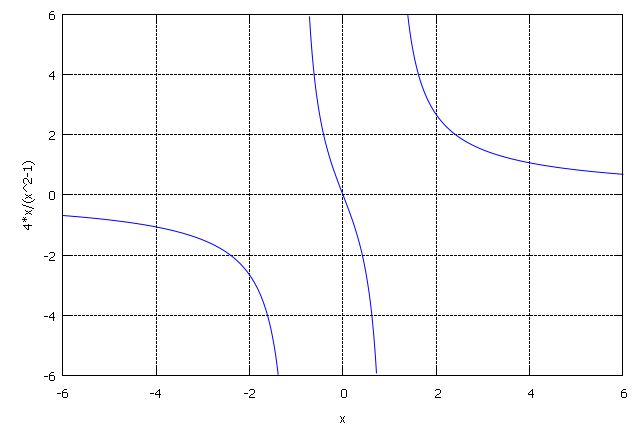
\includegraphics[scale=0.8,bb = 0 0 200 100, draft, type=eps]{/media/antalcides/Antalcides-EXT/maletin/ua12016/asignaturas/talleres/lyx_mathway/figuras/8_media_ANTALCIDES____talleresmat_pegado17.png}\caption{Trazado de una gr�fica}

\label{fig7} 
\end{figure}

\hecho 

\begin{ejercicios propuestos} 

\item[\bf Consejo.]\emph{ Una de las aplicaciones m�s �tiles de las
derivadas es a los problemas de optimizaci�n. En dichos problemas
se trata, por lo general, de calcular el m�ximo o el m�nimo absolutos
de una magnitud. Hay una gran variedad de problemas que responden
a este esquema y con frecuencia tienen contenido geom�trico o econ�mico
o f�sico. Por ello cada uno de estos ejercicios requiere un estudio
particular.}

\emph{Los siguientes consejos pueden ser �tiles:}\\
\emph{$\bullet$\ Entiende bien el problema. Haz, si es posible,
un dibujo o un esquema.}\\
\emph{$\bullet$\ Elige las variables y la magnitud, $Q$, que tienes
que optimizar.}\\
\emph{$\bullet$\ Estudia las relaciones entre las variables para
expresar la magnitud $Q$ como funci�n de una sola de ellas, $Q=f(x)$.}\\
\emph{$\bullet$\ Las condiciones del problema deben permitir establecer
el dominio de $f$.}\\
\emph{$\bullet$\ Estudia la variaci�n del signo de la derivada de
$f$ en su dominio para calcular m�ximos y m�nimos absolutos por aplicaci�n
de la proposici�n \ref{extremoabs}. }

%\setcounter{propuesto}{195}
\propuesto Dado un punto $P=(a,b)$ situado en el primer cuadrante
del plano, determina el segmento con extremos en los ejes coordenados
y que pasa por $P$ que tiene longitud m�nima.

\textbf{Observaci�n.} La soluci�n de este ejercicio tambi�n resuelve
el problema de calcular la longitud de la escalera m�s larga que,
llevada en posici�n horizontal, puede pasar por la esquina que forman
dos corredores de anchuras respectivas $a$ y $b$.

\propuesto Demuestra que entre todos los rect�ngulos con un per�metro
dado, el que tiene mayor �rea es un cuadrado.

\propuesto Determina el rect�ngulo con lados paralelos a los ejes
coordenados, inscrito en la elipse de ecuaci�n ${\displaystyle \frac{x^{2}}{a^{2}}+\frac{y^{2}}{b^{2}}=1}$,
y que tenga �rea m�xima.

\textbf{Observaci�n.} Los dos ejercicios anteriores se han resuelto
en el cap�tulo 1 usando la desigualdad de las medias. �Qu� m�todo
te parece mejor?

\propuesto Calcula el �rea m�xima de un rect�ngulo que tiene dos
v�rtices sobre una circunferencia y su base est� sobre una cuerda
dada de dicha circunferencia.

\propuesto Encuentra un punto $P$ de la circunferencia $\,x^{2}+y^{2}=1\,$
con coordenadas positivas y tal que el tri�ngulo cuyos v�rtices son
$(0,0)$ y las intersecciones de la tangente a la circunferencia en
$P$ con los ejes coordenados tenga �rea m�nima.

\propuesto Calcula un punto $(u,v)$ ($u>0,v>0$) de la elipse de
ecuaci�n $\,\dfrac{x^{2}}{9}+\dfrac{y^{2}}{4}=1\,$ tal que la tangente
a la elipse en dicho punto determine con los ejes un segmento de longitud
m�nima.

\propuesto Calcula el �rea de la elipse de m�nima �rea circunscrita
a un rect�ngulo dado. Recuerda que el �rea de una elipse de semiejes
$s$, $t$ es igual a $\pi st$.

\propuesto %
\begin{minipage}[t]{0.55\textwidth}%
 La figura representa un espejo rectangular en el que se ha partido
una esquina. Las dimensiones del espejo son $\overline{AB}=3$, $\overline{AC}=5$
y las de la esquina rota son las que se indican en la figura donde
se supone que $a$ es un valor conocido. Se pide calcular un punto
$P$ sobre la l�nea de corte de forma que el espejo de v�rtices $A,X,P,Y$
tenga �rea m�xima. �Para qu� valor de $a$ se verifica que el espejo
de mayor �rea es un cuadrado? %
\end{minipage}%
\begin{minipage}[t]{0.4\textwidth}%
\vspace{0pt}
 \flushright 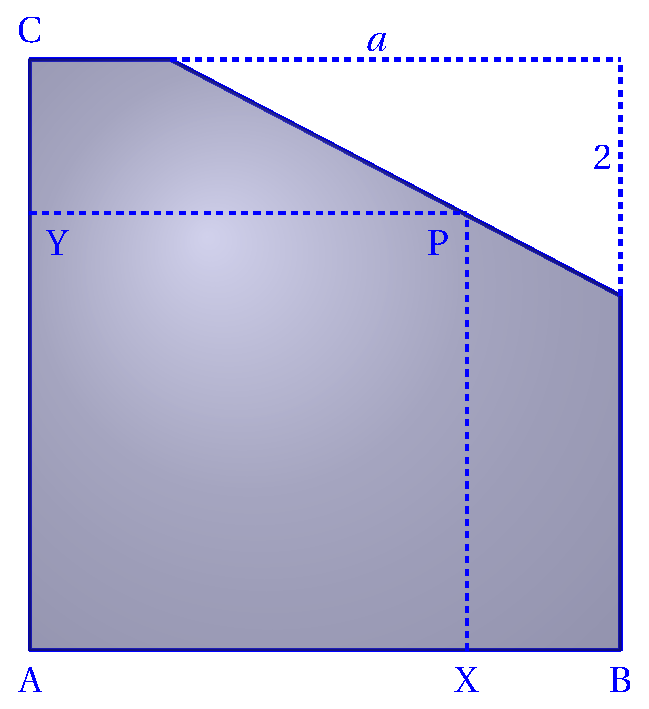
\includegraphics[scale=0.5]{52_home_antalcides_Calculo_pdf_espejo.pdf}%
\end{minipage}

\propuesto Se quiere construir una caja sin tapa con una l�mina met�lica
rectangular cortando cuadrados iguales en cada esquina y doblando
hacia arriba los bordes. Halla las dimensiones de la caja de mayor
volumen que puede construirse de tal modo si los lados de la l�mina
rectangular miden: a) 10\,cm. y %
\mbox{%
10\,cm.%
} b) 12\,cm. y 18\,cm.

\propuesto Calcula las dimensiones (radio y altura) de una lata cil�ndrica
de un litro de capacidad cuya superficie total sea m�nima.

\propuesto Calcula las dimensiones (radio y altura) de una lata cil�ndrica
de un litro de capacidad cuyo costo de producci�n sea m�nimo. Se supone
que no se desperdicia aluminio al cortar los lados de la lata, pero
las tapas de radio $r$ se cortan de cuadrados de lado $2r$ por lo
que se produce una p�rdida de metal.

\propuesto Se necesita construir un dep�sito de acero de 500 m$^{3}$,
de forma rectangular con base cuadrada y sin tapa. Tu trabajo, como
ingeniero de producci�n, es hallar las dimensiones del dep�sito para
que su costo de producci�n sea m�nimo.

\propuesto Halla el volumen del cilindro circular recto m�s grande
que puede inscribirse en una esfera de radio ($a>0$).

\propuesto Halla el volumen del cilindro circular recto m�s grande
que puede inscribirse en un cono circular recto de altura $h$ y radio
$r$ conocidos.

\propuesto Halla el volumen del cono circular recto m�s grande que
puede inscribirse en una esfera de radio ($a>0$).

\propuesto La resistencia de una viga de madera de secci�n rectangular
es proporcional a su anchura y al cuadrado de su altura. Calcula las
dimensiones de la viga m�s resistente que puede cortarse de un tronco
de madera de radio $r$.

\propuesto Calcula la distancia m�nima del punto $(6,3)$ a la par�bola
de ecuaci�n %
\mbox{%
$y=x^{2}$.%
}

\propuesto Una empresa tiene 100 casas para alquilar. Cuando la renta
es de 80 libras al mes, todas las casas est�n ocupadas. Por cada 4
libras de incremento de la renta una casa queda deshabitada. Cada
casa alquilada supone a la empresa un coste de 8 libras para reparaciones
diversas. �Cu�l es la renta mensual que permite obtener mayor beneficio?

\propuesto Una empresa produce semanalmente 300 bicicletas de monta�a
que vende �ntegramente al precio de 600 euros cada una. Tras un an�lisis
de mercados observa que si var�a el precio, tambi�n var�an sus ventas
(de forma continua) seg�n la siguiente proporci�n: por cada 7 euros
que aumente o disminuya el precio de sus bicicletas, disminuye o aumenta
la venta en 3 unidades. 

{[}a){]} 
\begin{enumerate}
\item �Puede aumentar el precio y obtener mayores ingresos? 
\item �A qu� precio los ingresos ser�n m�ximos? 
\end{enumerate}
\propuesto En la orilla de un r�o de 100 metros de ancho est� situada
una planta el�ctrica y en la orilla opuesta, y a 500 metros r�o arriba,
se est� construyendo una f�brica. Sabiendo que el r�o es rectil�neo
entre la planta y la f�brica, que el tendido de cables a lo largo
de la orilla cuesta a 9 euros cada metro y que el tendido de cables
sobre el agua cuesta a 15 euros cada metro, �cu�l es la longitud del
tendido m�s econ�mico posible entre la planta el�ctrica y la f�brica?.

\propuesto Se proyecta un jard�n en forma de sector circular de radio
$R$ y �ngulo central $\theta$ (medido en radianes). El �rea del
jard�n ha de ser $A$ fija. �Qu� valores de $R$ y $\theta$ hacen
m�nimo el per�metro del jard�n?.

\propuesto Se corta un alambre de longitud $L$ formando un c�rculo
con uno de los trozos y un cuadrado con el otro. Calcula por d�nde
se debe cortar para que la suma de las �reas de las dos figuras sea
m�xima o sea m�nima.

\propuesto Dados dos puntos $A$ y $B$ situados en el primer cuadrante
del plano, calcula cu�l es el camino m�s corto para ir de $A$ a $B$
pasando por un punto del eje de abscisas.

\propuesto Se desea construir una ventana con forma de rect�ngulo
coronado de un semic�rculo de di�metro igual a la base del rect�ngulo.
Pondremos cristal blanco en la parte rectangular y cristal de color
en el semic�rculo. Sabiendo que el cristal coloreado deja pasar la
mitad de luz (por unidad de superficie) que el blanco, calcula las
dimensiones de la ventana para conseguir la m�xima luminosidad si
se ha de mantener un per�metro constante dado.

\propuesto Se desea confeccionar una tienda de campa�a c�nica de
un volumen determinado. Calcula sus dimensiones para que la cantidad
de lona necesaria sea m�nima.

\propuesto En una l�mina circular de radio $R$ se recorta un sector
circular de �ngulo $\vartheta$ y con �l se construye un cono. Calcula
el valor de $\vartheta$ para que el volumen del cono as� construido
sea m�ximo.

\propuesto Se desea construir un silo, con un volumen $V$ determinado,
que tenga la forma de un cilindro rematado por una semiesfera. El
costo de construcci�n (por unidad de superficie) es doble para la
semiesfera que para el cilindro (la base es gratis). Calcula las dimensiones
�ptimas para minimizar el costo de construcci�n.

\propuesto Demuestra que de todos los tri�ngulos is�sceles que se
pueden circunscribir a una circunferencia de radio $r$, el de �rea
m�nima es el equil�tero de altura $3r$.

\propuesto Se considera la elipse $\,\dfrac{x^{2}}{a^{2}}+\dfrac{y^{2}}{b^{2}}=1$.
Calcula el tri�ngulo is�sceles de �rea m�xima inscrito en dicha elipse,
que tiene un v�rtice en el punto $(0,b)$ y base paralela al eje de
abscisas.

\propuesto Con una cuerda de longitud $L$, con un nudo corredizo
en uno de sus extremos, rodeamos una columna circular de radio $R$
haciendo pasar el otro extremo por el nudo. Calcula la m�xima distancia
posible del extremo libre al centro de la columna.

\propuesto Est�s en el desierto con tu veh�culo situado en un punto
cuyas coordenadas son $A=(0,40)$ y tienes que ir a otro punto $C=(28,0)$
(la unidad de medida es la milla terrestre). Del punto $A$ al origen
$O=(0,0)$ y de �ste al punto $C$ hay una carretera asfaltada. Pero
tambi�n, para ir de $A$ a $C$, puedes hacer parte o todo el camino
sobre la arena. En carretera tu velocidad es de 75 millas por hora;
y sobre la arena de 45 millas por hora. �Qu� camino debes seguir para
llegar lo antes posible a $C$?

\propuesto Calcula las dimensiones del rect�ngulo de mayor �rea que
puede inscribirse en un tri�ngulo equil�tero cuyo lado mide 2 cent�metros.
Se supone que el rect�ngulo se apoya sobre un lado del tri�ngulo.

\propuesto El principio de Fermat afirma que la luz viaja de un punto
$A$ a otro punto $B$ siguiendo la trayectoria en la que se invierte
el menor tiempo posible. Supongamos que el eje de abscisas, $y=0$,
separa dos medios en los que la luz viaja a distinta velocidad (por
ejemplo, aire y agua). Sea $c$ la velocidad de la luz en el semiplano
superior $y>0$ y sea $\frac{3}{4}c$ la velocidad correspondiente
al semiplano inferior $y<0$. Calcular el punto de dicho eje por el
que pasar� el rayo que viaje desde el punto $A=(-4,3)$ al $B=(3,-4)$.

\propuesto %
\begin{minipage}[t]{0.5\textwidth}%
 \vspace{0pt}
 Calcula la posici�n del punto $P=(x,0)$ en la figura de la derecha,
donde $A=(0,1)$ y $B=(2+\sqrt{3},2)$, para que el �ngulo $\theta$
sea m�ximo. �Cu�l es dicho valor m�ximo de $\theta$? Justifica con
detalle lo que haces. %
\end{minipage}%
\begin{minipage}[t]{0.45\textwidth}%
\vspace{8pt}
 \hspace{1cm} 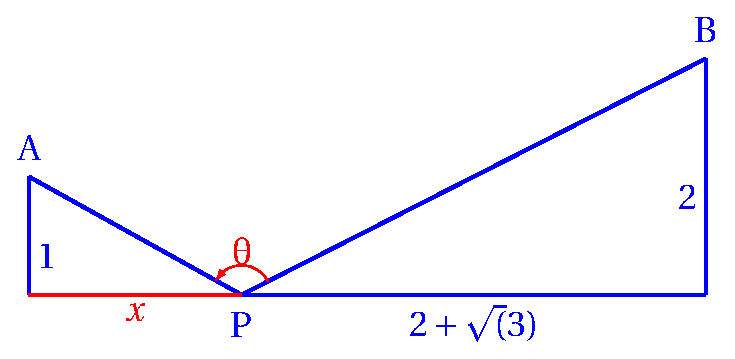
\includegraphics[scale=0.5]{53_home_antalcides_Calculo_pdf_punto-p.pdf}%
\end{minipage}

\bigskip{}

\emph{Uno de los resultados m�s �tiles del c�lculo diferencial son
las Reglas de L'H�pital que permiten resolver las indeterminaciones
en el c�lculo de l�mites.}

\propuesto Calcula el l�mite en el punto $a$ que en cada caso se
indica de las funciones siguientes: %que se suponen definidas en $]0,\pi/2[$.
\[
\begin{array}{ll}
\dis f(x)=(\sen x+\cos x)^{1/x},\ \ a=0; & \dis f(x)=(1+\tg x)^{1/x^{2}},\ \ a=0\\
\dis f(x)=(\cot x)^{\sen\,x},\ \ a=0; & \dis f(x)=\left(\cos^{2}x+\frac{x^{2}}{2}\right)^{1/x^{2}},\ \ a=0\\
\rule{0mm}{7mm}\dis f(x)=(1+\sen x)^{\cotg x},\ \ a=0; & \dis f(x)=\frac{\log(\sen x)}{(\pi-2x)^{2}},\ \ a=\pi/2\\
\rule{0mm}{7mm}\dis f(x)=\frac{x-\arctg x}{\sen^{3}x},\ \ a=0; & \dis f(x)=\frac{(\tg x)(\arctg x)-x^{2}}{x^{6}},\ \ a=0\\
\rule{0mm}{7mm}\dis f(x)=\dfrac{\e^{x}-\cos\sqrt{2\,}x-x}{\tg^{2}x},\ \ a=0; & \dis f(x)=\left(\frac{\sen x}{x}\right)^{1/(1-\cos x)},\ \ a=0
\end{array}
\]

\propuesto Justifica que para todo $r\en\R$ y para todo $s>0$ se
verifica que: 
\[
\Lim{\dfrac{(\log x)^{r}}{x^{s}}}{x}{+\infty}=0,\quad\Lim{\dfrac{x^{r}}{\e^{sx}}}{x}{+\infty}=0,\quad\limrgt{x^{s}\vert\log x\vert^{r}}{x}{0}=0.
\]

\propuesto Calcula el l�mite en el punto $a$ que en cada caso se
indica de las funciones $\,f:\R^{+}\rightarrow\R$. 
\[
f(x)=\frac{x^{2}\sen1/x}{\log x},\ \ a=+\infinity;\qquad f(x)=\sen\sqrt{1+x}-\sen\sqrt{x},\ \ a=+\infinity
\]
\[
f(x)=\sen x\,\sen\frac{1}{x},\ \ a=0,\ a=+\infinity;\qquad f(x)=\left(\cos\frac{\pi}{x+2}\right)^{x^{2}},\ \ a=+\infinity
\]

\propuesto Sea $\,g:\R\rightarrow\R$ derivable en \R \ y dos veces
derivable en 0 siendo, adem�s, $g(0)=0$. Definamos $\,f:\R\rightarrow\R$
por ${\displaystyle {\,f(x)=\frac{g(x)}{x}}}$\ si $\,x\neq0$, $f(0)=g\tl(0)$.
Estudia la derivabilidad de $\,f$. �Es $\,f\tl$ continua en 0?.

\propuesto Sean $\,f,g:]-1,\infty[\rightarrow\R$ las funciones definidas
por 
\[
f(x)=\frac{\log(1+x)}{x},\ f(0)=1;\ \ \ g(x)=\e^{f(x)}
\]
Calcula las derivadas primera y segunda de $f$ y $g$ en $0$ y deduce
el valor del l�mite 
\[
\lim_{x\to0}\frac{(1+x)^{1/x}-\e+\dfrac{\e}{2}x}{x^{2}}
\]

\propuesto Sea $f:]-1/2,+\infty[\rightarrow\R$ dada por ${\displaystyle {f(x)=(x+\e^{x})^{\frac{1}{x}}}}$
para $x\neq0$, y $f(0)=\e^{2}$. Estudia la continuidad y derivabilidad
de $f$ en cero.

\propuesto Estudia la derivabilidad de las siguientes funciones. 
\begin{enumerate}
\item $f:\R^{+}\rightarrow\R$, dada por ${\displaystyle f(x)=x^{1/(x^{2}-1)}}$,
y $f(1)=\sqrt{\e}$. 
\item $f:]-1/2,+\infty[\rightarrow\R$, dada por ${\displaystyle f(x)=(x+\e^{x})^{1/x}}$
y $f(0)=\e^{2}$. 
\item $f:[0,+\infty[\rightarrow\R$ dada por $f(x)=(1+x\,\log x)^{1/x}$,
y $f(0)=0$. 
\item $f:]-\pi/2,\pi/2[\rightarrow\R$ dada por $f(x)=\left(\dfrac{\sen x}{x}\right)^{1/x^{2}}$
y $f(0)=\e^{-1/6}.$ 
\item $f:\R\rightarrow\R$, dada por ${\displaystyle f(x)=\left(1+x^{2}\right)^{\sen(1/x)},\ \ f(0)=1}.$ 
\item \func{f}{{]}-\pi/2,\pi/2{[}}\ dada por $f(x)=\left(\dfrac{2-2\cos x}{x^{2}}\right)^{1/x}$
para $x\neq0$ y $f(0)=1.$ 
\end{enumerate}
\propuesto Calcula los l�mites 
\begin{alignat*}{2}
 & \lim_{x\to0}\left(\dfrac{1}{\sen^{2}x}-\dfrac{1}{x^{2}}\right) & \qquad & \lim_{x\to1}\left(\dfrac{1}{\log x}-\dfrac{1}{x-1}\right)\\
 & \lim_{x\to0}\dfrac{x\e^{2x}+x\e^{x}-2\e^{2x}+2\e^{x}}{(\e^{x}-1)^{3}} &  & \lim_{x\to+\infty}\left(\dfrac{\pi}{2}-\arctg x\right)^{\frac{1}{\log x}}\\
 & \lim_{x\to0}\dfrac{\log\left(\dfrac{\sen x}{x}\right)}{(\log(1+x))^{2}} &  & \lim_{x\to0}\left(\dfrac{\tg x}{x}\right)^{1/x^{2}}\\
 & \lim_{x\to0}\dfrac{x\log(1+\sen2x)\arctg(\sen^{3}x)}{(\e^{x}-1)(1-\cos^{2}(\tg^{2}x))} &  & \lim_{x\to0}\dfrac{\arctg x-\sen x}{x(1-\cos x)}\\
 & \lim_{x\to0}\dfrac{\arctg(\arcsen x^{2})}{(\e^{2x}-1)\log(1+2x)} &  & \lim_{x\to0}\left(\frac{3\sen x-3\,x\,\cos x}{x^{3}}\right)^{1/x}
\end{alignat*}
\textbf{Sugerencia.} Pueden usarse las reglas de L'H�pital pero es
conveniente realizar previamente alguna transformaci�n.

\propuesto Explica si es correcto usar las reglas de L'H�pital para
calcular los l�mites: 
\[
\lim_{x\to+\infty}\frac{x-\sen x}{x+\sen x};\qquad\lim_{x\to\,0}\frac{x^{2}\sen(1/x)}{\sen x}.
\]

\smallskip{}

\emph{El teorema de los ceros de Bolzano, junto con el teorema de
Rolle, permiten determinar en muchas ocasiones el n�mero de ceros
reales de una funci�n.}

Se dice que \textbf{una funci�n polin�mica} $P(x)$ \textbf{tiene
un cero de orden} $k\ge1$ en un punto $a$, si el valor de $P$ y
el de sus derivadas hasta la de orden $k-1$ en $a$ es cero, y la
derivada de orden $k$ de $P$ no se anula en $a$. Los ceros de orden
$1$ se llaman \textbf{ceros simples}. El Teorema Fundamental del
�lgebra dice que una funci�n polin�mica de grado $n$ (en general,
con coeficientes complejos) tiene $n$ ra�ces reales o complejas \emph{contando
cada ra�z tantas veces como indica su orden}. Recuerda tambi�n que
las ra�ces complejas de un polinomio con coeficientes reales vienen
por pares de ra�ces complejas conjugadas.

\smallskip{}

\propuesto Prueba que una funci�n polin�mica de grado $n$ coincide
con su polinomio de Taylor de orden $n$ centrado en un punto cualquiera
$a$.

\propuesto Prueba que una funci�n polin�mica $P$ tiene un cero de
orden $k$ en $a$ si, y s�lo si, puede escribirse de la forma $P(x)=(x-a)^{k}Q(x)$,
donde $Q(x)$ es una funci�n polin�mica que no se anula en $a$.

\propuesto Calcula el n�mero de ceros y la imagen de la funci�n \func{f}{\R},
$\ f(x)=x^{6}-3x^{2}+2$.

\propuesto Calcula el n�mero de soluciones de la ecuaci�n $3\log x-x=0$.

\propuesto Estudia el n�mero de soluciones reales de la ecuaci�n
$3x^{5}+5x^{3}-30x=\alpha$ seg�n los valores de $\alpha$.

\propuesto Determina el n�mero de soluciones reales de la ecuaci�n
$2x^{3}-3x^{2}-12x=m$ seg�n el valor de $m$.

\propuesto Justifica que la ecuaci�n $\ x^{2}=x\sen x+\cos x\ $
tiene exactamente dos soluciones reales.

\propuesto Sea $f$ una funci�n polin�mica que tiene un m�ximo relativo
en $(-3,5)$, un m�nimo relativo en $(1,1)$ y un m�ximo relativo
en $(4,7)$ y no tiene m�s puntos cr�ticos. �Cu�ntos ceros reales
tiene $f$? \propuesto Prueba por medio del teorema de Rolle que
la ecuaci�n $5x^{4}-4x+1=0$ tiene alguna soluci�n en $[0,1]$.

\propuesto Estudia el n�mero de ceros reales de la funci�n $f(x)=2^{x}-1-x^{2}$.

\propuesto Prueba que entre cada dos soluciones reales de la ecuaci�n
$\e^{x}\sen x=1$ hay al menos una soluci�n real de la ecuaci�n $\e^{x}\cos x=-1$.

\propuesto Sean $\,a_{0},a_{1},\ldots,a_{n}$ n�meros reales. Prueba
que para alg�n $x\in[0,1]$ se verifica que ${\dis\sum_{k=0}^{n}a_{k}x^{k}=\sum_{k=0}^{n}\dfrac{a_{k}}{k+1}}$.

\propuesto Sea $f$ una funci�n polin�mica y sea $a<b$. Justifica
que, {\em contando cada cero tantas veces como su orden}, si $f(a)f(b)<0$
el n�mero de ceros de $f$ en $]a,b[$ es impar; y si $f(a)f(b)>0$
dicho n�mero (caso de que haya alg�n cero) es par. Deduce que si $f$
tiene grado $n$, es condici�n necesaria y suficiente para que $f$
tenga $n$ ra�ces reales distintas que su derivada tenga $n-1$ ra�ces
reales distintas $c_{1}<c_{2}<\cdots<c_{n-1}$ y que para $\alpha<c_{1}$
suficientemente peque�o y para $\beta>c_{n-1}$ suficientemente grande,
los signos de los n�meros $f(\alpha),f(c_{1}),f(c_{2}),\dots,f(c_{n-1}),f(\beta)$
vayan alternando.

\propuesto Determina para qu� valores de $\alpha$ la funci�n polin�mica
$3x^{4}-8x^{3}-6x^{2}+24x+\alpha$ tiene cuatro ra�ces reales distintas.

\propuesto Dado $n\en\N$, sea $\,f(x)=(x^{2}-1)^{n}\ \ (x\en\R)$.
Prueba que la derivada $k$-�sima ($1\leq k\leq n$) de $f$ tiene
exactamente $k$ ra�ces reales distintas en el intervalo $]-1,1[$.

\propuesto Dado\nN, sea $f_{n}(x)=1-x+\dfrac{x^{2}}{2}-\dfrac{x^{3}}{3}+\cdots+(-1)^{n}\dfrac{x^{n}}{n}$.
Prueba que si $n$ es impar la ecuaci�n $f_{n}(x)=0$ tiene una �nica
soluci�n y ninguna si $n$ es par.

\smallskip{}

\emph{El teorema del valor medio permite acotar el incremento de una
funci�n por el incremento de la variable y una cota de la derivada.
Esto da lugar a muchas desigualdades interesantes. Por otra parte,
algunas de las desigualdades m�s �tiles son consecuencia de la convexidad.
Los siguientes ejercicios tratan de ello.}

\smallskip{}

\propuesto Sean $0<x<y$. Prueba que:

a)\ $\dfrac{y-x}{1+y^{2}}<\arctg y-\arctg x<\dfrac{y-x}{1+x^{2}}$.

b)\ $\rule{0mm}{6mm}\dfrac{y-x}{y}<\log y-\log x<\dfrac{y-x}{x}$.

\propuesto Sean $n\in\N$, $n\ge2$ y $0<a<b$. Prueba que 
\[
na^{n-1}(b-a)<b^{n}-a^{n}<nb^{n-1}(b-a)
\]
\textbf{Aplicaci�n}. Haciendo ${\dis\,a\!=\!1+\dfrac{1}{n+1},\ b=\!1+\dfrac{1}{n}}$,
primero en la desigualdad de la derecha y despu�s en la desigualdad
de la izquierda, deduce que: 
\[
\left(1+\frac{1}{n}\right)^{\!n}<\left(1+\frac{1}{n+1}\right)^{\!n+1},\qquad\left(1+\frac{1}{n+1}\right)^{\!n+2}<\left(1+\frac{1}{n}\right)^{\!n+1}
\]

\propuesto Prueba que para todo $x>-1$ se verifica que 
\[
\dfrac{x}{x+1}\leq\log(1+x)
\]
�Cu�ndo se da la igualdad en la desigualdad anterior?

\propuesto Supuesto que $a>0$, demuestra que $-a\,\e\log x\leqslant x^{-a}$
para todo $x>0$.

\propuesto Dado $\alpha\in]0,1[$, prueba que $\,x^{\alpha}<\alpha x+1-\alpha\,$
para todo $x\en\R^{+}\setminus\{1\}$.

Deduce que, dados $p>0$ y $q>0$ tales que $1/p+1/q=1$, entonces
para todos $a>0$ y $b>0$ se verifica que $ab\le\dfrac{a^{p}}{p}+\dfrac{b^{q}}{q}$.
�Cu�ndo se da la igualdad?

\propuesto Sean $0<a<b$. Prueba que si $b\leq\e$ entonces $a^{b}\!<b^{a}$,
y si $\e\leq a$ entonces %
\mbox{%
$b^{a}\!<a^{b}$.%
} �Qu� puede decirse si $a<\e<b$?.

\textbf{Sugerencia}. Considera la funci�n ${\displaystyle {\,x\mapsto\frac{\log x}{x}}}$.

\propuesto�Hay alg�n n�mero $a>0$ que verifique que $\,a^{x/a}\geq x\,$
para todo $x\en\R^{+}$? �Cu�l es dicho n�mero?

\propuesto Prueba que para todo $x\in]0,\pi/2[$ se verifica que
\[
i)\ 1-\frac{x^{2}}{2}<\cos x\,;\quad ii)\ \frac{2x}{\pi}<\sen x<x<\tg x
\]

\propuesto Dados $a,b\en\Rp$ con $a\neq b$, prueba que para todo
$x\en\R$ se verifica la desigualdad: 
\[
\left(\dfrac{a+x}{b+x}\right)^{b+x}\ms{-8mu}>\!\dfrac{a}{b}.
\]

\propuesto \textbf{Desigualdad de Jensen}. Sea $f:I\rightarrow\R$
una funci�n convexa en el intervalo $I$, y sea $n\en\N$, $n\ge2$.
Dados n�meros $\alpha_{k}>0$, $x_{k}\en I$ tales que $\sum_{k=1}^{n}\alpha_{k}=1$,
prueba que: 
\[
f\left(\sum_{k=1}^{n}\alpha_{k}x_{k}\right)\leq\sum_{k=1}^{n}\alpha_{k}f(x_{k}).
\]
Adem�s, si $f$ es estrictamente convexa, la desigualdad anterior
es estricta siempre que al menos dos de los puntos $x_{k}$ sean distintos.

\textbf{Sugerencia}. Es suficiente considerar el caso $n=2$ y proceder
por inducci�n.

\propuesto Sean $x_{k}$, $\alpha_{k}$, donde $1\leq k\leq n$,
n�meros positivos verificando que $\sum_{k=1}^{n}\alpha_{k}=1$. Usando
la convexidad de la funci�n $\,x\mapsto-\log x\,$ demuestra la desigualdad:
\[
x_{1}^{\alpha_{1}}x_{2}^{\alpha_{2}}\cdots x_{n}^{\alpha_{n}}\le\sum_{k=1}^{n}\alpha_{k}x_{k}
\]
�Cu�ndo se da la igualdad?

\propuesto Sean $p,q$ n�meros reales positivos tales que $1/p+1/q=1$.

a) Prueba que $\ ab\leqslant\dfrac{a^{p}}{p}+\dfrac{b^{q}}{q}\ $
y la igualdad ocurre si, y s�lo si, $a^{p}=b^{q}$.

b) Dado $\vz=(z_{1},z_{2},\dots,z_{n})\en\R^{n}$ y $s>0$, definamos
$\norma{z}_{s}=\dis\left(\sum_{i=1}^{n}|z_{i}|^{s}\!\right)^{\!\!1/s}$.
Prueba que para todo $\vx=(x_{1},x_{2},\dots,x_{n})$ y todo $\vy=(y_{1},y_{2},\dots,y_{n})\,$
en $\R^{n}$ se verifica la \textbf{desigualdad de H�lder}: 
\[
\sumaf{i=1}{n}\modulo{x_{i}y_{i}}\leqslant\norma{x}_{p}\norma{y}_{q}.
\]
�Cu�ndo se da la igualdad?

\textbf{Sugerencias.} El punto a) puede hacerse como consecuencia
del ejercicio anterior. Para b) h�gase $a=\dfrac{|x_{i}|}{\norma{x}_{p}},b=\dfrac{|y_{i}|}{\norma{y}_{q}}$
en la desigualdad del punto a).

\propuesto Sea $f$ es una funci�n derivable en un intervalo $I$.
Prueba que $f$ es convexa en $I$ si, y s�lo si, la gr�fica de $f$
queda siempre por encima de la recta tangente en cualquier punto,
es decir, para todo par de puntos $x,a\en I$ se verifica que %
\mbox{%
$f(x)\geqslant f(a)+f\tl(a)(x-a)$%
}.

\medskip{}

\emph{Los teoremas de Taylor\textendash Young y de Taylor se usan
para obtener aproximaciones polinomiales de una funci�n dada y para
calcular valores aproximados con precisi�n prefijada.}

\medskip{}

\propuesto Calcula una funci�n polin�mica $\varphi$ tal que ${\displaystyle \lim_{x\to\,0}\frac{\sqrt[3]{1+x}-\varphi(x)}{x^{5}}}=0$.

\propuesto Calcula una funci�n polin�mica $\,\varphi\,$ tal que
${\displaystyle \lim_{x\to\,0}\frac{\log\arctg(x+1)-\varphi(x)}{x^{2}}}=0.$

\propuesto Prueba que las �nicas funciones $n$ veces derivables
con derivada de orden $n$ constante son las funciones polin�micas
de grado menor o igual que $n$.

\propuesto Prueba que el polinomio de Taylor de orden $n$ de una
funci�n $f$ es el �nico polinomio $P(x)$ de grado menor o igual
que $n$ que verifica que $f(x)=P(x)+o(x-a)^{n}$.

\propuesto Sea \func{f}{{]}-\pi/2,\pi/2{[}} la funci�n dada
para $x\in]-\pi/2,\pi/2[$, $x\neq0$, por: 
\[
f(x)=\dfrac{\log(1+\sen x)-\sen x}{\sen^{2}x},
\]
y $f(0)=-1/2$. Calcula el polinomio de Taylor de orden 3 de $f$
en $0$.

\propuesto Sea \func{f}{{]}-1,+\infty{[}} la funci�n dada para
$x\neq0$ por: 
\[
f(x)=\dfrac{\arctg(\log(1+x))}{\log(1+x)},
\]
y $f(0)=1$. Calcula el polinomio de Taylor de orden 3 de $f$ en
$0$.

\propuesto Calcula, usando un desarrollo de Taylor conveniente, un
valor aproximado del n�mero real $\alpha$ con un error menor de $10^{-3}$
en cada uno de los casos siguientes: 
\[
a)\ \alpha=\sqrt[3]{7}\quad b)\ \alpha=\sqrt{\e}\quad c)\ \alpha=\sen\frac{1}{2}\quad d)\ \alpha=\sen(61^{\circ})
\]

\emph{Una de las aplicaciones m�s comunes de las derivadas es el trazado
de gr�ficas. Para trazar la gr�fica de una funci�n $f$ se debe tener
en cuenta:}\\
\textbf{\emph{1.}}\emph{ Propiedades de simetr�a o de periodicidad
de $f$.}\\
\textbf{\emph{2.}}\emph{ Los puntos en que se anula la primera o la
segunda derivada de $f$ y los puntos en los que $f$ no es derivable.}\\
\textbf{\emph{3.}}\emph{ Los intervalos en que \fder{f}\ tiene
signo constante. Lo que nos informa del crecimiento y decrecimiento
de $f$ y tambi�n de la naturaleza de los puntos singulares (m�ximos
y m�nimos locales).}\\
\textbf{\emph{4.}}\emph{ Los intervalos en que la derivada segunda
tiene signo constante. Lo que nos informa de la convexidad y concavidad,
as� como de los puntos de inflexi�n.}\\
\textbf{\emph{5.}}\emph{ Hallar las as�ntotas.}\\
\textbf{\emph{As�ntota vertical}}\emph{. La recta $\,x=c\,$ es una
as�ntota vertical de la gr�fica de $f$ si alguno de los l�mites laterales
de $f$ en $\,c\,$ es infinito.}\\
\textbf{\emph{As�ntota horizontal}}\emph{. La recta $\,y=L\,$ es
una as�ntota horizontal de la gr�fica de $f$ si $f$ tiene l�mite
en $+\infty$ o en $-\infty$ igual a $\,L$.}\\
\textbf{\emph{As�ntota oblicua}}\emph{. Si $f$ es una funci�n racional
con el grado del numerador una unidad mayor que el grado del denominador,
entonces puede escribirse de la forma 
\[
f(x)=mx+b+g(x)
\]
donde $\dis\lim_{x\to+\infty}g(x)=0$. En tal caso la recta $\,y=mx+b\,$
es una as�ntota oblicua de la gr�fica de $f$.}\\
\textbf{\emph{6.}}\emph{ Dibujar m�ximos, m�nimos, puntos de inflexi�n,
cortes con los ejes y cortes con las as�ntotas.}

\propuesto Dibuja las gr�ficas de las funciones siguientes:

\begin{tabular}{l@{\mbox{$\ms{45mu}$}}l}
a)\ $f(x)=3x^{5}-5x^{3}+2$  &
b)\ $\dis f(x)=\frac{x^{2}+1}{x^{2}-1}$ \tabularnewline
c)\ $\dis f(x)=\frac{x^{2}-2x+2}{x-1}$  &
d)\ $f(x)=|x|^{2x}$ \tabularnewline
e)\ $\rule{0mm}{6mm}f(x)=\sqrt[3]{x^{2}}(x-2)^{2}$  &
f)\ $f(x)=x^{4}-4x^{3}+10$\tabularnewline
g)\ \rule{0mm}{6mm} $\dis{f(x)=\frac{x^{2/3}}{(x-6)^{2/3}}}$  &
h)\ $f(x)=2x^{2}\log|x|-5x^{2},\ f(0)=0$ \tabularnewline
i) \ $\dis f(x)=\frac{x^{2}-x-2}{x-3}$  &
j)\ \rule{0mm}{6mm} $\dis{f(x)=\dfrac{2x^{2}-3x+5}{(x+1)(x-2)}}$ \tabularnewline
k)\ $f(x)=\log(2+\sen x)$  &
\tabularnewline
\end{tabular}

\propuesto La figura de abajo muestra la gr�fica de una funci�n $f$
dos veces derivable. Estudia el signo de la primera y la segunda derivada
de $f$ en cada uno de los puntos indicados, suponiendo que la gr�fica
representa el siguiente fen�meno..\\[2cm]\medskip{}
 %
\begin{minipage}[t]{0.55\textwidth}%
\vspace{50pt}

Si suponemos que la gr�fica de la derecha representa la distancia
desde el origen de un sistema de referencia de un m�vil que se mueve
a lo largo de una l�nea recta en un tiempo $t$. Indica, de acuerdo
con el estudios de sus derivadas a la vista de la gr�fica y de forma
aproximada contesta lo siguiente: 

a)\ Cu�ndo se est� alejando o acercando al origen. \\
b)\ Cu�ndo est� acelerando y cu�ndo est� frenando. %
\end{minipage}%
\begin{minipage}[t]{0.35\textwidth}%
\vspace{0pt}
\flushright 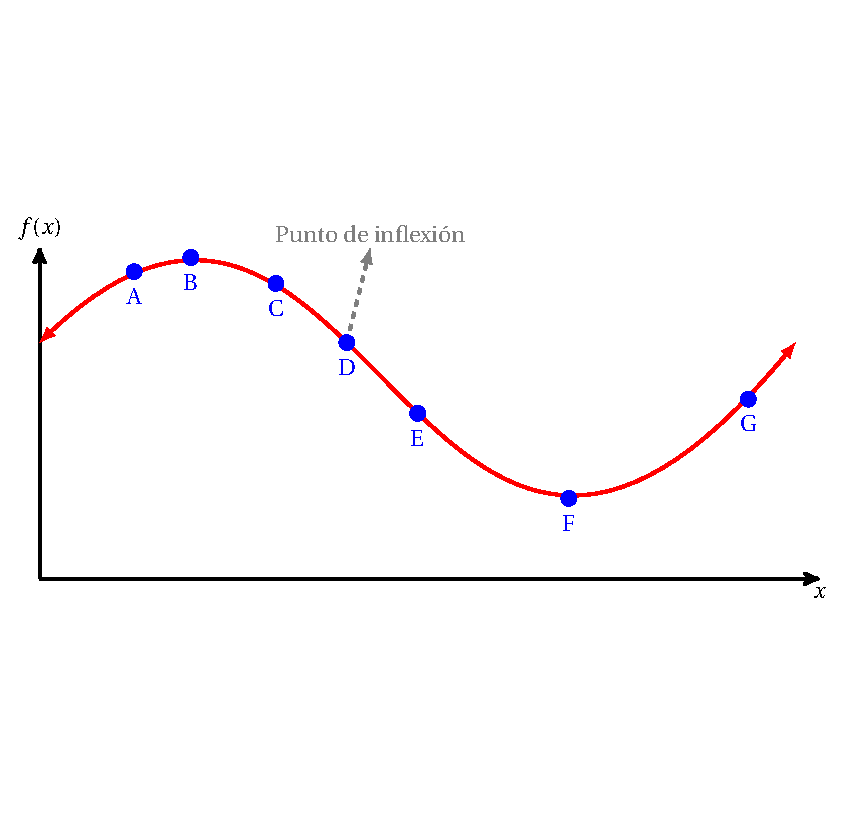
\includegraphics[scale=0.5]{54_home_antalcides_Calculo_pdf_estudio.pdf}%
\end{minipage}

\propuesto %
\begin{minipage}[t]{0.35\textwidth}%
 \vspace{15pt}
 La figura de la derecha muestra la gr�fica de una funci�n y de su
derivada. Debes identificar cada una de ellas y explicar las relaciones
entre ambas gr�ficas. %
\end{minipage}%
\begin{minipage}[t]{0.57\textwidth}%
\vspace{0pt}
 \flushright 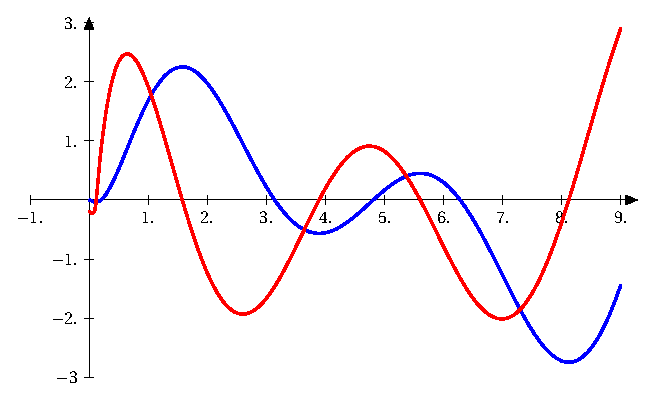
\includegraphics[scale=0.5]{55_home_antalcides_Calculo_pdf_derivadas.pdf}%
\end{minipage}

\propuesto %
\begin{minipage}[t]{0.35\textwidth}%
 \vspace{20pt}
 La figura de la derecha muestra la gr�fica de una funci�n y de sus
dos primeras derivadas. Debes identificar cada una de ellas y explicar
las relaciones entre dichas gr�ficas. %
\end{minipage}%
\begin{minipage}[t]{0.6\textwidth}%
\vspace{-10pt}
 \flushright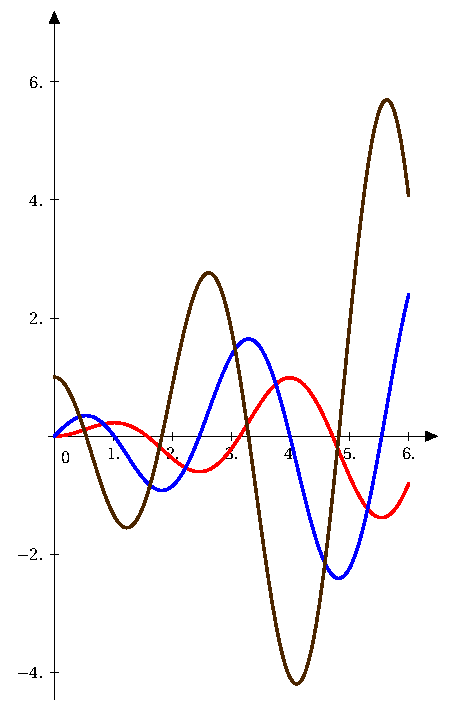
\includegraphics[width=6cm,height=4cm]{56_home_antalcides_Calculo_pdf_derivadas2.pdf}%
\end{minipage}

\propuesto Traza la gr�fica de una funci�n $f$ dos veces derivable
en \R, sabiendo que:

a) La gr�fica de $f$ pasa por los puntos $(-2,2),(-1,1),(0,0),(1,1),(2,2)$.

b) $f\tl$ es positiva en los intervalos $]-\infty,-2[$ y $]0,2[$,
y es negativa en $]-2,0[$ y $]2,+\infty[$.

c)\ $f^{\prime\prime}$ es negativa en los intervalos $]-\infty,-1[$
y $]1,+\infty[$, y es positiva en el intervalo $]-1,1[$.

\propuesto a)\ �Es cierto que los puntos donde se anula la derivada
segunda son puntos de inflexi�n?

b)\ �Qu� puedes decir de los puntos de inflexi�n de una funci�n polin�mica
de grado 2 o 3?

Justifica tus respuestas.

\propuesto �Es cierto que la gr�fica de toda funci�n polin�mica de
grado par tiene tangente horizontal en alg�n punto? �Y si el grado
es impar? Justifica tus respuestas.

\bigskip{}

\emph{Consideraremos ahora el problema de hallar el m�ximo o m�nimo
absolutos de una funci�n continua $f$ en un intervalo cerrado $[a,b]$.
Para ello puede seguirse el siguiente procedimiento:}

\textbf{\emph{Paso 1}}\emph{. Hallar todos los puntos $x$ de $[a,b]$
que o bien son puntos singulares de $f$ o son puntos en los que $f$
no es derivable.}\\
\textbf{\emph{Paso 2}}\emph{. Calcular el valor de $f$ en cada uno
de los puntos obtenidos en el Paso 1 y tambi�n en $a$ y en $b$.}\\
\textbf{\emph{Paso 3}}\emph{. Comparar los valores obtenidos en el
Paso 2. El mayor de todos ello ser� el m�ximo absoluto de $f$ en
$[a,b]$ y el menor ser� el m�nimo absoluto de $f$ en $[a,b]$.}

\bigskip{}

\propuesto Calcula los valores m�ximo y m�nimo de las siguientes
funciones en los intervalos que se indican: 
\begin{enumerate}
\item $f(x)=x^{3}-x^{2}-8x+1$ en el intervalo $[-2,2]$. 
\item $f(x)=\dfrac{x+1}{x^{2}+1}$ en el intervalo $[-1,2]$. 
\item $f(x)=\dfrac{1}{2}(\sen^{2}x+\cos x)+2\sen x-x$ en el intervalo $[0,\pi/2]$. 
\item $f(x)=\sqrt[3]{x^{2}}(5-2x)$ en el intervalo $[-1,2]$. 
\item $f(x)=-x^{3}+12x+5$ en el intervalo $[-3,3]$. 
\end{enumerate}
\propuesto Para cada n�mero real $t$ sea $f(x)=-\frac{1}{3}x^{3}+t^{2}x$.
Calcula, para cada valor de $t\in[-1,1]$, el m�nimo valor de $f(x)$
en el intervalo $[0,1]$.

\bigskip{}

\emph{Cuando una funci�n no est� definida en un intervalo cerrado
hay que estudiar el signo de la derivada si queremos calcular m�ximos
o m�nimos absolutos cuya existencia habr� que justificar.}

\bigskip{}

\propuesto Definamos $f(x)=5x^{2}+\alpha x^{-5}$, donde $\alpha>0$
es una constante. Calcula el valor m�s peque�o de $\alpha$ tal que
$f(x)\ge21$ para todo $x>0$.

\propuesto Calcula el m�nimo valor de $\dis\sum_{k=1}^{n}(x-a_{k})^{2}$
donde $\,a_{1},a_{2},\cdots a_{n}$ son n�meros reales dados.

\propuesto Calcula la imagen de \func{f}{\Rp}\ dada por $\ {\displaystyle {f(x)=x^{\frac{1}{x}}}}$.

\propuesto Sea \func{f}{\R}\ la funci�n definida por $\,\dis{f(x)=\e^{-1/x^{2}}}$
para $x\neq0$, y $f(0)=0$. Estudia la continuidad y derivabilidad
de $f$ y calcula su imagen.

\propuesto Dado $a\neq0$, definamos, para $x\neq1/a$, la funci�n:
\[
f(x)=\arctan a+\arctan x-\arctan\dfrac{a+x}{1-ax}.
\]
Calcula la imagen de $f$.

\bigskip{}

\emph{Acabamos esta larga relaci�n con algunos ejercicios que me ha
parecido que no encajaban propiamente en ninguno de los apartados
anteriores.}

\bigskip{}

\propuesto Supongamos que $f$ es una funci�n derivable en $a$ con
$f(a)\neq0$. Calcula el l�mite: 
\[
\lim_{x\to0}\left(\dfrac{f(a+x)}{f(a)}\right)^{\!\frac{1}{x}}.
\]

\propuesto Sea $f$ dos veces derivable en $a$. Calcula el l�mite:
\[
\lim_{h\to0}\dfrac{f(a+h)+f(a-h)-2f(a)}{h^{2}}.
\]
\propuesto Sea \func{f}{{[}a,b{]}}\ derivable y $f\tl$ creciente.
Prueba que la funci�n $g:]a,b]\rightarrow\R$ dada para todo $x\in]a,b]$
por 
\[
g(x)=\frac{f(x)-f(a)}{x-a}
\]
es creciente.

\propuesto Sea $f:[0,1]\rightarrow\R$ una funci�n derivable verificando
que $f(0)=0$ y que $\abs{f\tl(x)}\le\abs{f(x)}$ para todo $x\in[0,1]$.
Prueba que $f(x)=0$ para todo $x\in[0,1]$.

\propuesto Sea \func{f}{{[}a,b{]}}\ continua en $[a,b]$ y
derivable dos veces en $]a,b[$. Supongamos que el segmento de extremos
$\,(a,f(a)),\ (b,f(b))\,$ corta a la gr�fica de $\,f$ en un punto
$\,(c,f(c))\,$ con $\,a<c<b.$ Demuestra que existe alg�n punto $d\!\in]a,b[\,$
tal que %
\mbox{%
$f\scd(d)=0.$%
}

Sugerencia. Interpreta gr�ficamente el enunciado.

\propuesto Justifica que existe una funci�n $g:\R\rightarrow\R$
derivable y que verifica que $\dis{g(x)+\e^{g(x)}=x}$ para todo $x\en\R$.
Calcula $g\tl(1)$ y $g\tl(1+\e)$.

\propuesto Sea $f:\R\rightarrow\R$ dada por $f(x)=x^{3}-3x^{2}+3x+17$.
Prueba que $f$ es una biyecci�n y estudia la derivabilidad de $f^{-1}$.

\propuesto Justifica que hay una funci�n derivable \func{\ff}{\R}\ tal
que para todo $x\en\R$ verifica que $(\ff(x))^{5}+\ff(x)+x=0$.

\propuesto Sea $f$ una funci�n derivable que no se anula en ning�n
punto. Justifica que la funci�n %
\mbox{%
$h(x)=\log|f(x)|$%
} es derivable y calcula su derivada.

\propuesto Sea $f:\R\rightarrow\R$ verificando que $f(x+y)=f(x)f(y)$
para todos $x,y\en\R$; $f(0)\neq0$ y $f$ es derivable en 0. Justifica
que $f$ es derivable en todo punto y hay un n�mero real $\alpha$
tal que %
\mbox{%
$\dis f(x)=\e^{\alpha x}$%
} para todo $x\en\R$.

\propuesto Sea $\,f:\R\rightarrow\R$ una funci�n dos veces derivable
y tal que para todo $x\en\R$ se verifica la igualdad $f\scd(x)+f(x)=0$.
Prueba que existen n�meros $\alpha,\beta\en\R$, �nicos, de manera
que $f(x)=\alpha\sen x+\beta\cos x$ para todo $x\en\R$.

Sugerencia. Define $h(x)=\alpha\sen x+\beta\cos x$ y considera la
funci�n 
\[
g(x)=(f(x)-h(x))^{2}+(f\tl(x)-h\tl(x))^{2}.
\]
Calcula $g\tl(x)$.

\propuesto Prueba la llamada ``f�rmula de Machin'': 
\[
\frac{\pi}{4}=4\arctan\frac{1}{5}-\arctan\frac{1}{239}.
\]
Sugerencia. Sea $A=\arctan1/5,\ B=4A-\pi/4$. Calcula $\tan B$.

Utiliza la f�rmula de Machin para calcular $\pi$ con cinco cifras
decimales exactas.

\propuesto Sea $f$ una funci�n polin�mica de grado $n$ tal que
$f^{(k)}(a)\geq0$ para $1\leq k\leq n$ y $f(a)>0$. Justifica que
si $f(c)=0$, entonces $c<a.$

\propuesto Sea $\,f\,$ derivable en $[a,b]$ con $f^{\,\prime}(a)=f^{\,\prime}(b)=0$.
Prueba que hay alg�n $z\en]a,b[$ tal que ${\displaystyle f^{\,\prime}(z)=\frac{f(z)-f(a)}{z-a}}.$

Sugerencia. Sea ${\displaystyle {g(x)=\frac{f(x)-f(a)}{x-a}}}$ para
$a<x\leq b$. Define convenientemente $g(a)$ y compara $g^{\,\prime}(b)$
con ${\displaystyle \frac{g(b)-g(a)}{b-a}}$.

\end{ejercicios propuestos}

\begin{ejercicios resueltos}

\resuelto Dado un punto $P=(a,b)$ situado en el primer cuadrante
del plano, determinar el segmento con extremos en los ejes coordenados
y que pasa por $P$ que tiene longitud m�nima.

\sol

\begin{minipage}[t]{0.5\textwidth}%
 En un ejercicio como este \emph{lo primero que hay que hacer es elegir
la variable} en funci�n de la cual vamos a calcular la longitud del
segmento $\overline{AB}$. Tomando como variable $\ff$, es decir,
la medida en radianes del �ngulo indicado en la figura, la longitud
del segmento $\overline{AB}$ viene dada por 
\[
f(\ff)=\frac{b}{\sen\ff}+\frac{a}{\cos\ff}\qquad(0<\ff<\pi/2)
\]
Debemos calcular el m�nimo absoluto de $f$. Tenemos que: %
\end{minipage}%
\begin{minipage}[t]{0.45\textwidth}%
\vspace{0pt}
  \flushright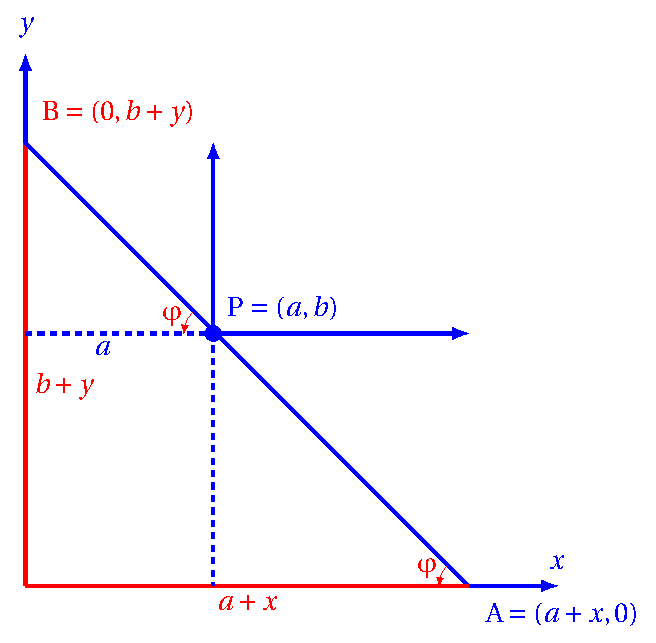
\includegraphics[scale=0.5]{57_home_antalcides_Calculo_pdf_resuelto6-1.pdf}%
\end{minipage}

\[
f\tl(\ff)=\frac{-b\,\cos\ff}{\sen^{2}\ff}+\frac{a\,\sen\ff}{\cos^{2}\ff}
\]
Se obtiene enseguida que $f\tl(\ff)$ se anula en un \emph{�nico}
punto $\ff_{0}\in]0,\pi/2[$ que viene dado por la condici�n $\dis\tg(\ff_{0})=\sqrt[3]{b/a}$.
Se justifica f�cilmente que $f$ tiene en $\ff_{0}$ un m�nimo absoluto.

En efecto, como $f\tl$ es continua y no se anula en los intervalos
$]0,\ff_{0}[$ y $]\ff_{0},\pi/2[$, debe tener signo constante en
ellos. Como $\Lim{f\tl(\ff)}{x}{0}=-\infty$, y $\Lim{f\tl(\ff)}{x}{\pi/2}=+\infty$
se sigue que: 
\[
\ff\in]0,\ff_{0}[\longrightarrow f\tl(\ff)<0,\quad\ff\in]\ff_{0},\pi/2[\longrightarrow f\tl(\ff)>0
\]
por tanto, $f$ es estrictamente decreciente en $]0,\ff_{0}]$ y estrictamente
creciente en $[\ff_{0},\pi/2[$, lo que implica que $f(\ff_{0})\leqslant f(\ff)$
para todo $\ff\en]0,\pi/2[$.

Para calcular la longitud m�nima $f(\ff_{0})$, basta tener en cuenta
que: 
\[
1+\tg^{2}(\ff_{0})=\frac{1}{\cos^{2}(\ff_{0})}=1+\sqrt[3]{\rule{0mm}{5mm}\left(\dis\frac{b}{a}\right)^{2}}\longrightarrow\frac{a}{\cos(\ff_{0})}=a^{2/3}\big(a^{2/3}+b^{2/3}\big)^{1/2}
\]
F�cilmente se obtiene ahora que $\dis\frac{b}{\sen(\ff_{0})}=b^{2/3}\big(a^{2/3}+b^{2/3}\big)^{1/2}$
con lo que la longitud m�nima buscada viene dada por: 
\[
f(\ff_{0})=\big(a^{2/3}+b^{2/3}\big)^{3/2}
\]

Otra forma de calcular la longitud del segmento $\overline{AB}$ consiste
en considerar la ecuaci�n general de las rectas que pasan por el punto
$P=(a,b)$. Dicha ecuaci�n general es de la forma $y=\lambda(x-a)+b$,
donde $\lambda$ es un par�metro. Las intersecciones de dicha recta
con los ejes son los puntos $A=(a-b/\lambda,0)$ y $B=(0,-a\lambda+b)$.
Por tanto, la longitud del segmento $\overline{AB}$ viene dada por:
\[
g(\lambda)=\sqrt{\left(a-\frac{b}{\lambda}\right)^{2}+(b-a\lambda)^{2}}\qquad(\lambda<0)
\]

Otra forma de calcular la longitud del segmento $\overline{AB}$ consiste
en introducir las variables $x$ e $y$ tales que $A=(a+x,0)$, $B=(0,b+y)$,
como se indica en la figura. La longitud del segmento $\overline{AB}$
viene dada por $H(x,y)=\sqrt{(a+x)^{2}+(b+y)^{2}}$. Esta funci�n,
aparentemente, depende de dos variables, pero dichas variables \emph{no
son independientes}, pues los puntos $A$, $P$ y $B$ est�n alineados.
Por semejanza de tri�ngulos se obtiene que $x/b=a/y$, por lo que
$y=(ab)/x$. En consecuencia, la longitud del segmento $\overline{AB}$
viene dada por: $h(x)=\sqrt{(a+x)^{2}+(b+(ab)/x)^{2}}\quad(x>0)$.

\sskip

Tanto si se usa la funci�n $g$ como la $h$, debemos obtener un m�nimo
absoluto y, como son ra�ces cuadradas, es suficiente que calculemos
el m�nimo absoluto de la funci�n radicando (las ra�ces respetan el
orden en \Rpo). Es decir, las funciones $g$ y $h$ alcanzan su m�nimo
absoluto en el mismo punto en que lo alcanzan las funciones:
\[
G(\lambda)=\left(a-\frac{b}{\lambda}\right)^{2}+(b-a\lambda)^{2}\quad(\lambda<0);\qquad H(x)=(a+x)^{2}+\left(b+\frac{ab}{x}\right)^{2}\quad(x>0)
\]
Comprueba que, de cualquier forma que lo hagas, vuelves a obtener
la soluci�n anterior.

\textbf{Comentario.} Una forma equivalente de enunciar este ejercicio
es la siguiente: Calcula la longitud de la escalera m�s larga que
llevada en posici�n horizontal puede pasar por la esquina que forman
dos corredores de anchuras respectivas $a$ y $b$.

Es evidente que la longitud de la escalera tiene que ser \emph{menor
o igual} que la longitud de \emph{cualquier} segmento $\overline{AB}$
como el de la figura. Por tanto, la longitud de la escalera \emph{m�s
larga} que puede pasar es igual a la \emph{longitud m�nima} del segmento
$\overline{AB}$.\hecho

\resuelto Determina el rect�ngulo con lados paralelos a los ejes
coordenados, inscrito en la elipse de ecuaci�n ${\displaystyle \frac{x^{2}}{a^{2}}+\frac{y^{2}}{b^{2}}=1}$,
y que tenga �rea m�xima.

\sol

\begin{minipage}[t]{0.5\textwidth}%
 \vspace{0pt}
 Por razones de simetr�a, es suficiente determinar el v�rtice del
rect�ngulo situado en el primer cuadrante. Si las coordenadas de dicho
v�rtice son $(x,y)$, entonces el �rea del rect�ngulo ser� igual a
$4xy$. Como el v�rtice debe estar en la elipse, sus coordenadas $x$
e $y$ deber�n satisfacer la igualdad ${\displaystyle \dfrac{x^{2}}{a^{2}}+\dfrac{y^{2}}{b^{2}}=1}$. %
\end{minipage}%
\begin{minipage}[t]{0.45\textwidth}%
\vspace{-15pt}
\flushright 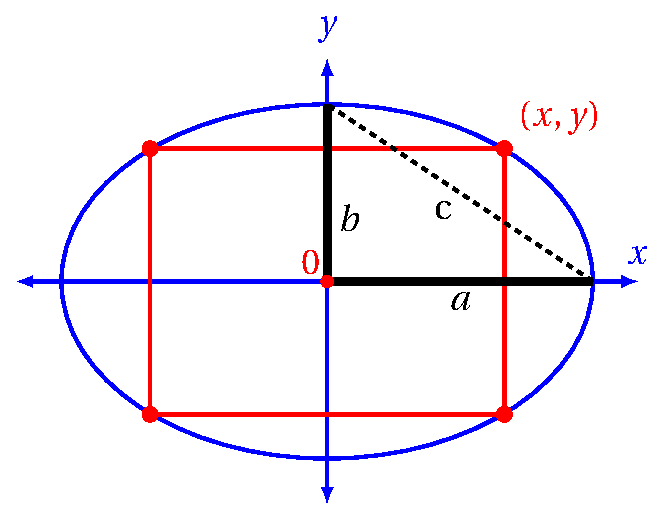
\includegraphics[scale=0.5]{58_home_antalcides_Calculo_pdf_resuelto6-2.pdf}%
\end{minipage}

Deducimos que $\,y=b\sqrt{1-\dfrac{x^{2}}{a^{2}}}$. Por tanto, se
trata de calcular el m�ximo absoluto de la funci�n $\,f(x)=x\,b\sqrt{1-\dfrac{x^{2}}{a^{2}}}$,
donde $0\leqslant x\leqslant a$.

Como se trata de una funci�n positiva, para calcular el valor en que
alcanza su m�ximo podemos elevarla al cuadrado. En definitiva, nuestro
problema es calcular el m�ximo absoluto de la funci�n $\,h(x)=x^{2}\left(1-\dfrac{x^{2}}{a^{2}}\right)$
en el intervalo $[0,a]$. Tenemos que 
\[
h\tl(x)=2x\left(1-\dfrac{x^{2}}{a^{2}}\right)+x^{2}\dfrac{-2x}{a^{2}}=2x-\dfrac{4x^{3}}{a^{2}}.
\]
Los puntos cr�ticos de $h$ son $x=0$ que corresponde a un m�nimo
y $x=\dfrac{a}{\sqrt{2}}$ que corresponde a un m�ximo absoluto (justificaci�n:
la funci�n $h(x)$ se anula en los extremos del intervalo $[0,a]$
y es positiva en $]0,a[$ por lo que su m�ximo absoluto en $[0,a]$
tiene que alcanzarse en un punto del intervalo abierto $]0,a[$ en
el cual debe anularse su derivada. Pero el �nico punto que cumple
estas condiciones es $a/\sqrt{2}$).

El rect�ngulo pedido es el que tiene de v�rtices $\left(\pm\dfrac{a}{\sqrt{2}},\pm\dfrac{b}{\sqrt{2}}\right)$,
y su �rea vale $2ab$.\hecho

\resuelto Calcula el �rea m�xima de un rect�ngulo que tiene dos v�rtices
sobre una circunferencia y su base est� sobre una cuerda dada de dicha
circunferencia.

\sol

\begin{minipage}[t]{0.5\textwidth}%
 \vspace{20pt}
 Sea $\rho$ el radio de la circunferencia y $\overline{BA}$ la cuerda.
Pongamos $A=(\rho\cos\alpha,\rho\sen\alpha)$ que es un dato conocido.
Observa que $-\pi/2<\alpha\leqslant0$. Hay que calcular un punto
$P=(\rho\cos\beta,\rho\sen\beta)$ por la condici�n de que el rect�ngulo
de la figura tenga m�xima �rea. La altura, $h$, del rect�ngulo viene
dada por %
\mbox{%
$h=\rho(\sen\beta-\sen\alpha)$,%
} y la base, $b$, por $b=2\rho\cos\beta$. Observa que la longitud
de la base del rect�ngulo no puede ser mayor que la longitud de la
cuerda $\overline{BA}$, lo que implica que $\cos\beta\le\cos\alpha=\cos(-\alpha)$.
Como el coseno es decreciente en el intervalo $[0,\pi/2]$,\linebreak{}
%
\end{minipage}%
\begin{minipage}[t]{0.45\textwidth}%
\vspace{-15pt}
  \flushright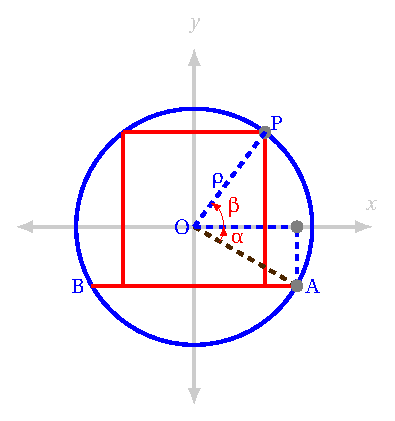
\includegraphics{59_home_antalcides_Calculo_pdf_resuelto6-3.pdf}%
\end{minipage}\vspace*{-0.5cm}

deber� ser $\beta\ge-\alpha$. Debemos calcular el m�ximo absoluto
de $2\rho^{2}\cos\beta(\sen\beta-\sen\alpha)$ donde $-\alpha\leqslant\beta\leqslant\pi/2$.Pongamos,
por comodidad, $\beta=x$ y prescindamos del factor $2\rho^{2}$.
Sea 
\[
f(x)=\cos x(\sen x-\sen\alpha)\qquad-\alpha\le x\le\pi/2\quad(\textrm{donde }-\pi/2<\alpha\le0)
\]
%Como la funci�n seno es estrictamente creciente en $[-\pi/2,\pi/2]$, y el coseno es positivo en dicho intervalo, la funci�n $f(x)$ es positiva en $[-\alpha,\pi/2]$. Adem�s, $f$ solamente se anula en el extremo $f(\pi/2)=0$.

Tenemos que $\,f\tl(x)=-\sen x(\sen x-\sen\alpha)+\cos^{2}x=-2\sen^{2}x+\sen\alpha\,\sen x+1$.
Haciendo $t=\sen x$ tenemos que $f\tl(x)=0$ equivale a que $-2t^{2}+t\,\sen\alpha+1=0$.
Esta ecuaci�n tiene dos ra�ces reales que vienen dadas por 
\[
t_{0}=\dfrac{\sen\alpha-\sqrt{\sen^{2}\alpha+8}}{4},\quad t_{1}=\dfrac{\sen\alpha+\sqrt{\sen^{2}\alpha+8}}{4}
\]
Adem�s, como 
\[
\modulo{\dfrac{\sen\alpha\pm\sqrt{\sen^{2}\alpha+8}}{4}}<\frac{1+\sqrt{9}}{4}=1
\]
Tenemos que $-1<t_{0}<0<t_{1}<1$. Por tanto, la derivada $f\tl$
se anula en dos �nicos puntos que vienen dados por: 
\[
\beta_{0}=\arcsen\left(\dfrac{\sen\alpha-\sqrt{\sen^{2}\alpha+8}}{4}\right),\quad\beta_{1}=\arcsen\left(\dfrac{\sen\alpha+\sqrt{\sen^{2}\alpha+8}}{4}\right)
\]
Tenemos que $-\pi/2<\beta_{0}<0<\beta_{1}<\pi/2$. Como $-2t^{2}+t\sen\alpha+1$
es una par�bola hacia abajo, toma valores positivos entre sus dos
ra�ces, es decir $-2t^{2}+t\sen\alpha+1>0$ para $t_{0}<t<t_{1}$.
Lo que implica que $f\tl(x)>0$ para $\beta_{0}<x<\beta_{1}$.

Como $f\tl(\pi/2)=\sen\alpha-1<0$ y$f\tl$ no se anula en $]\beta_{1},\pi/2]$,
concluimos que $f\tl$ debe ser negativa en dicho intervalo y, por
tanto $f$ es estrictamente decreciente en $[\beta_{1},\pi/2]$.

A la vista de los resultados anteriores, debemos distinguir dos casos:

a) $-\alpha\le\beta_{1}$. En este caso, $f$ es creciente en $[-\alpha,\beta_{1}]$
y decreciente en $[\beta_{1},\pi/2]$, por lo que el m�ximo absoluto
de $f$ en $[-\alpha,\pi/2]$ se alcanza en $\beta_{1}$.

b) $\beta_{1}<-\alpha$. En este caso, $f$ es estrictamente decreciente
en $[-\alpha,\pi/2]$ por lo que el m�ximo absoluto de $f$ en $[-\alpha,\pi/2]$
se alcanza en $-\alpha$.

Finalmente, se comprueba con facilidad que la desigualdad $0\le-\alpha\le\beta_{1}$,
equivale a $0\le-\sen\alpha\le1/\sqrt{3}$, esto es, $-\arcsen(1/\sqrt{3})\le\alpha\le0$.

Observa que si $\alpha=0$, entonces $\beta=\arcsen(\sqrt{2}/2)=\pi/4$,
es decir, en este caso el rect�ngulo es la mitad del cuadrado inscrito
en la circunferencia.\hecho

\resuelto Encuentra un punto $P$ de la circunferencia $\,x^{2}+y^{2}=1\,$
con coordenadas positivas y tal que el tri�ngulo cuyos v�rtices son
$(0,0)$ y las intersecciones de la tangente a la circunferencia en
$P$ con los ejes coordenados tenga �rea m�nima.

\sol

\begin{minipage}[t]{0.6\textwidth}%
 \vspace{0pt}
 Sean $(s,t)$ las coordenadas de $\,P$. La ecuaci�n de la recta
tangente a la circunferencia $\,x^{2}+y^{2}=1\,$ en $\,P\,$ es $\,xs+yt=1$,
cuyos cortes con los ejes son los puntos %
\mbox{%
$A=(0,1/t)$,%
} $B=(1/s,0)$. Por tanto el �rea del tri�ngulo $AOB$ es igual a 
\[
\dfrac{1}{2}\dfrac{1}{s\,t}=\dfrac{1}{2}\dfrac{1}{s\sqrt{1-s^{2}}}
\]
%
\end{minipage}%
\begin{minipage}[t]{0.35\textwidth}%
\vspace{-5pt}
 \flushright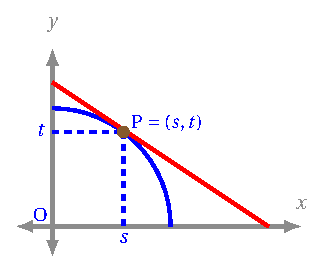
\includegraphics{60_home_antalcides_Calculo_pdf_resuelto6-4.pdf}%
\end{minipage}

Para calcular su valor m�nimo, como se trata de una funci�n positiva,
podemos elevarla al cuadrado para simplificar los c�lculos. En definitiva,
nuestro problema se reduce a calcular el m�nimo de la funci�n $\,f(s)=\dfrac{1}{s^{2}(1-s^{2})}$
en el intervalo $]0,1[$.

Derivando tenemos $\,f\tl(s)=2\dfrac{2s^{2}-1}{s^{3}(1-s^{2})^{2}}$.
Por tanto el �nico cero de la derivada en el intervalo $]0,1[$ es
$\,s=1/\sqrt{2}$. Como para $0<s<1/\sqrt{2}$ se tiene que $f\tl(s)<0$,
y para $1/\sqrt{2}<s<1$ es $f\tl(s)>0$, deducimos que en el punto
$1/\sqrt{2}$ hay un m�nimo absoluto de $f$. El punto $P=(1/\sqrt{2},1/\sqrt{2})$
es, por tanto, el que proporciona el tri�ngulo de m�nima �rea.\hecho

\resuelto Se quiere construir una caja sin tapa con una l�mina met�lica
rectangular cortando cuadrados iguales en cada esquina y doblando
hacia arriba los bordes. Halla las dimensiones de la caja de mayor
volumen que puede construirse de tal modo si los lados de la l�mina
rectangular miden: a) 10\,cm. y %
\mbox{%
10\,cm.%
} b) 12\,cm. y 18\,cm.

\sol

\begin{minipage}[t]{0.55\textwidth}%
 \vspace{0pt}
 Sean $\,a\,$ y $\,b\,$ las longitudes de los lados de la l�mina
y $\,x\,$ la longitud del lado del cuadrado que se cortar� en cada
esquina. Supongamos que $a\le b$. El volumen de la caja resultante
es $\,f(x)=(a-2x)(b-2x)x$. Se trata de calcular el m�ximo absoluto
de la funci�n $f$ en el intervalo $[0,a/2]$. Derivando resulta %
\mbox{%
$f\tl(x)=12x^{2}-4(a+b)x+ab$.%
} Los ceros de la derivada son %
\end{minipage}%
\begin{minipage}[t]{0.4\textwidth}%
\vspace{-20pt}
 \flushright 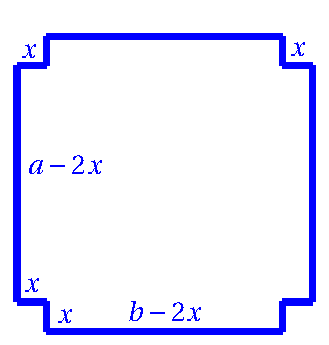
\includegraphics[scale=0.5]{61_home_antalcides_Calculo_pdf_resuelto6-5.pdf}%
\end{minipage}

\[
\alpha=\frac{1}{6}\left(a+b-\sqrt{a^{2}+b^{2}-ab}\right),\quad\beta=\frac{1}{6}\left(a+b+\sqrt{a^{2}+b^{2}-ab}\right)
\]
F�jate que: 
\[
a^{2}+b^{2}-ab>a^{2}+b^{2}-2ab=(b-a)^{2}\geq0\quad\longrightarrow\quad\sqrt{a^{2}+b^{2}-ab}>b-a.
\]
Deducimos que las ra�ces de $f\tl$ son \emph{reales}. Veamos si dichas
ra�ces est�n en el intervalo $[0,a/2]$. Tenemos que: 
\[
\alpha=\frac{1}{6}\left(a+b-\sqrt{a^{2}+b^{2}-ab}\right)<\frac{1}{6}(a+b-(b-a))=\frac{a}{3}
\]
Tambi�n: 
\[
a^{2}+b^{2}-ab<a^{2}+b^{2}+2ab=(a+b)^{2}\quad\longrightarrow\quad\sqrt{a^{2}+b^{2}-ab}<a+b\quad\longrightarrow\quad\alpha>0.
\]
Por tanto $0<\alpha<a/3$ y $\alpha\in]0,a/2[$. Comprobemos que $\beta\ge a/2$.
\[
\frac{1}{6}\left(a+b+\sqrt{a^{2}+b^{2}-ab}\right)\ge\frac{a}{2}\quad\Longleftrightarrow\quad\sqrt{a^{2}+b^{2}-ab}\ge2a-b
\]
Si $2a-b\le0$, est� desigualdad es trivialmente cierta. Supongamos
que $2a-b>0$. En tal caso, elevando al cuadrado ambos lados, la desigualdad
anterior equivale a la siguiente: 
\[
a^{2}+b^{2}-ab\ge4a^{2}-4ab+b^{2}\quad\Longleftrightarrow\quad3a(b-a)\ge0
\]
Lo cual es cierto porque se ha supuesto que $a\le b$, luego $\beta\not\in]0,a/2[$.

Por el teorema de Weierstrass, sabemos que $f$ alcanza un m�ximo
absoluto en alg�n punto $x_{0}\in[0,a/2]$. Como $f(0)=f(a/2)=0$
y $f(x)>0$ para $0<x<a/2$, debe ser $x_{0}\in]0,\pi/2[$. En consecuencia,
$x_{0}$ tambi�n es un extremo relativo de $f$ en $[0,\pi/2]$ por
lo que la derivada de $f$ debe anularse en $x_{0}$. Pero el �nico
punto del intervalo $[0,a/2]$ en el que se anula la derivada de $f$
es $\alpha$. Concluimos as� que $x_{0}=\alpha$.

Con unos sencillos c�lculos se obtiene 
\[
f(\alpha)=\frac{1}{54}(-2a^{3}+3a^{2}b+3ab^{2}-2b^{3}+2(a^{2}-ab+b^{2})^{3/2})
\]

\textbf{Comentario.} Otra forma de razonar este ejercicio, algo m�s
indirecta pero con la que te ahorras trabajo, es como sigue.

Como $f(0)=f(a/2)=0$, podemos aplicar el teorema de Rolle, para obtener
que la derivada de $f$ tiene que anularse en alg�n punto de $]0,a/2[$.
Adem�s, $f$ tiene que alcanzar en un punto $x_{0}$ de $[0,a/2]$
un m�ximo absoluto y como, evidentemente, $x_{0}\in]0,a/2[$, deducimos
que $f\tl$ debe anularse en $x_{0}$. Luego o bien es $x_{0}=\alpha$
o es $x_{0}=\beta$. El criterio de la derivada segunda nos permite
salir de dudas. Tenemos que $f\scd(x)=-4(a+b-6x)$. Con ello,
\[
f\scd(\alpha)=-4(a+b-6\alpha)=-4\sqrt{a^{2}+b^{2}-ab},\ f\scd(\beta)=-4(a+b-6\beta)=4\sqrt{a^{2}+b^{2}-ab}
\]
Por tanto, $f\scd(\alpha)<0$ y $f\scd(\beta)>0$. Deducimos as� que
el punto $\alpha$ est� en el intervalo $]0,a/2[$ y en �l la funci�n
$f$ alcanza su m�ximo absoluto en $[0,a/2]$.

Alternativamente, puedes estudiar el signo de la primera derivada.
Escribiendo $f\tl(x)=12(x-\alpha)(x-\beta)$, se sigue que $f\tl(x)<0$
si $x\in]\alpha,\beta[$ y $f\tl(x)>0$ si $x<\alpha$ o si $x>\beta$.
Deducimos que $f$ es creciente en el intervalo $]-\infty,\alpha]$,
decreciente en el intervalo $[\alpha,\beta]$ y creciente en $[\beta,+\infty[$.
Luego en $\alpha$ hay un m�ximo relativo. Ahora hay que justificar
que $\alpha$ est� en $[0,a/2]$ y que es el punto donde $f$ alcanza
su m�ximo absoluto en dicho intervalo.\hecho

\resuelto Calcular las dimensiones (radio y altura) de una lata cil�ndrica
de un litro de capacidad cuya superficie total sea m�nima.

\sol Sea $r$ el radio y $h$ la altura medidos en dec�metros. Como
el volumen es %
\mbox{%
1 dcm$^{3}$,%
} tenemos que $\pi r^{2}h=1$, de donde $h=\dfrac{1}{\pi r^{2}}$.
La superficie total de la lata es $f(r)=2\pi r^{2}+2\pi rh=2\pi r^{2}+\dfrac{2}{r}$.
Se trata, por tanto, de calcular el m�ximo absoluto de $f(r)$ cuando
$r>0$. Derivando, $f\tl(r)=4\pi r-\dfrac{2}{r^{2}}=2\dfrac{2\pi r^{3}-1}{r^{2}}$.
Deducimos que la derivada tiene un �nico cero real $\alpha=\dfrac{1}{\sqrt[3]{2\pi}}$.
Como para $0<r<\alpha$ es $f\tl(r)<0$, se sigue que $f$ es decreciente
en el intervalo $]0,\alpha]$; y como para $\alpha<r$ es $f\tl(r)>0$,
se sigue que $f$ es creciente en el intervalo $[\alpha,+\infty[$.
En consecuencia $f(\alpha)\leqslant f(r)$ para todo $r>0$. As�,
las dimensiones de la lata con m�nima superficie lateral son $r=\dfrac{1}{\sqrt[3]{2\pi}}\approxeq0,542\textrm{dcm}$,
y $h\approxeq1,1\textrm{dcm}$.\hecho

%\pagebreak

\resuelto Hallar el volumen del cilindro circular recto m�s grande
que puede inscribirse en una esfera de radio ($a>0$).

\sol

\begin{minipage}[t]{0.55\textwidth}%
 \vspace{0pt}
 La relaci�n entre el radio de la esfera $a$, el radio de la base
del cilindro, $r$, y la altura del cilindro, $h$, viene dada, como
se deduce de la figura, por $a^{2}=r^{2}+\dfrac{h^{2}}{4}$. El volumen
del cilindro viene dado por $\pi r^{2}h=\pi\dfrac{4a^{2}-h^{2}}{4}h$.
El problema se reduce a calcular el m�ximo absoluto de $f(h)=4a^{2}h-h^{3}$
en el intervalo $[0,2a]$. Tenemos que $f\tl(h)=4a^{2}-3h^{2}$. Como
la funci�n $f$ es positiva en $]0,2a[$ y se anula en los extremos
del intervalo, deducimos, por un razonamiento ya varias veces repetido,
que el �nico cero que tiene la derivada en el intervalo $]0,2a[$,\linebreak{}
%
\end{minipage}%
\begin{minipage}[t]{0.4\textwidth}%
\vspace{0pt}
\flushright 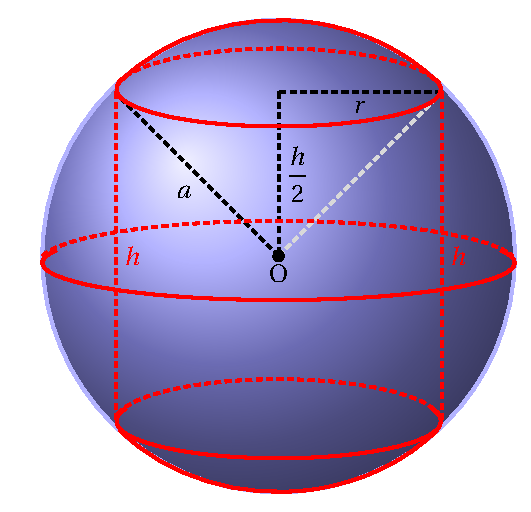
\includegraphics[scale=0.5]{62_home_antalcides_Calculo_pdf_resuelto6-6.pdf}%
\end{minipage}\vspace{-0.5cm}

es decir, el punto, $\alpha=2a/\sqrt{3}$, corresponde a un m�ximo
absoluto de $f$ en $[0,2a]$.\hecho

\resuelto Hallar el volumen del cono circular recto m�s grande que
puede inscribirse en una esfera de radio ($a>0$).

\sol

\begin{minipage}[t]{0.55\textwidth}%
 \vspace{0pt}
 Sean $r$ y $h$ el radio y la altura del cono. Tenemos que 
\[
(h-a)^{2}+r^{2}=a^{2}
\]
es decir, $\,r^{2}=a^{2}-(h-a)^{2}$. El volumen del cilindro viene
dado por $\,\dfrac{1}{3}\pi r^{2}h=\dfrac{1}{3}\pi(a^{2}-(h-a)^{2})h$.
El problema se reduce a calcular el m�ximo absoluto de 
\[
f(h)=\dfrac{1}{3}\pi(a^{2}-(h-a)^{2})h=\dfrac{\pi}{3}h^{2}(2a-h)
\]
%
\end{minipage}%
\begin{minipage}[t]{0.4\textwidth}%
\vspace{5pt}
 \flushright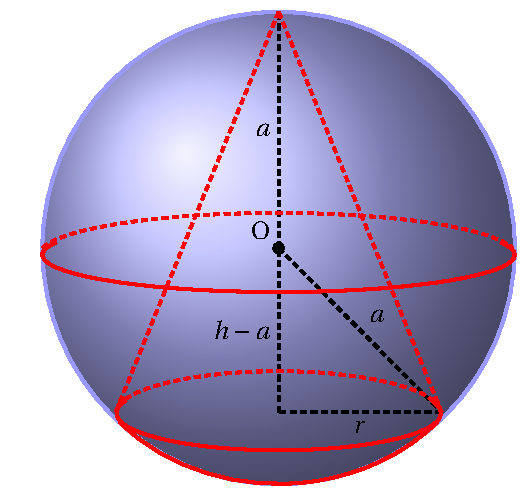
\includegraphics[scale=0.5]{63_home_antalcides_Calculo_pdf_resuelto6-7.pdf}%
\end{minipage}

en el intervalo $[0,2a]$. Tenemos que $f\tl(h)=\dfrac{\pi}{3}(4a-3h)h$.
De donde se deduce enseguida que el cilindro de mayor volumen que
puede inscribirse en la esfera dada es el de altura $h=4a/3$ y radio
$r=\dfrac{8a^{2}}{9}$; y su volumen es igual a $\dfrac{32a^{3}\pi}{81}$.\hecho

\resuelto Hallar el volumen del cilindro circular recto m�s grande
que puede inscribirse en un cono circular recto de altura $H$ y radio
$R$ conocidos.

\sol

\begin{minipage}[t]{0.6\textwidth}%
 \vspace{0pt}
 Sean $r$ y $h$ el radio y la altura del cilindro. Por ser los tri�ngulos
$OAB$ y $DCB$ semejantes, tenemos que $\dfrac{r}{R}=\dfrac{H-h}{H}$,
de donde, $\,h=H(1-r/R)$. El volumen del cilindro viene dado por
$\,\pi r^{2}h=\pi Hr^{2}\left(1-\dfrac{r}{R}\right)$. El problema
se reduce a calcular el m�ximo absoluto de $f(r)=\pi Hr^{2}\left(1-\dfrac{r}{R}\right)$
en el intervalo $[0,R]$. Tenemos que $f\tl(r)=\dfrac{H\pi r(2R-3r)}{R}$.
De donde se deduce enseguida que el cilindro de mayor volumen que
puede inscribirse en el cono dado es el de radio $r=2R/3$ y altura
$h=H/3$; y su volumen es igual a $\dfrac{4\pi R^{2}H}{27}$.\hecho %
\end{minipage}%
\begin{minipage}[t]{0.35\textwidth}%
\vspace{15pt}
 \flushright 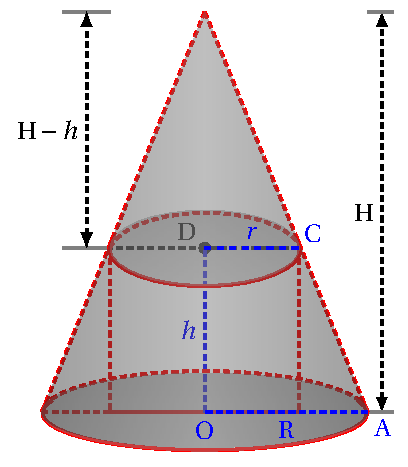
\includegraphics[scale=0.6]{64_home_antalcides_Calculo_pdf_resuelto6-8.pdf}%
\end{minipage}

\resuelto La resistencia de una viga de madera de secci�n rectangular
es proporcional a su anchura y al cuadrado de su altura. Calcular
las dimensiones de la viga m�s resistente que puede cortarse de un
tronco de madera de radio $R$.

\sol

\begin{minipage}[t]{0.6\textwidth}%
 \vspace{0pt}
 Sean $x$ e $y$ las coordenadas del v�rtice superior derecho de
la viga. Ser� $\,x^{2}+y^{2}=R^{2}$. Nos dicen que la resistencia
de la viga viene dada por una funci�n de la forma $\,kxy^{2}$ donde
$\,k\,$ es una constante. El problema consiste en calcular el m�ximo
absoluto de $f(x)=\,kx(R^{2}-x^{2})$ en el intervalo $[0,R]$. Tenemos
que $f\tl(x)=k(R^{2}-3x^{2})$. De donde se deduce enseguida que la
viga m�s resistente se obtiene para $\,x=R/\sqrt{3}$, e $\,y=\sqrt{\dfrac{2}{3}}R$.\hecho %
\end{minipage}%
\begin{minipage}[t]{0.35\textwidth}%
\vspace{-10pt}
 \flushright 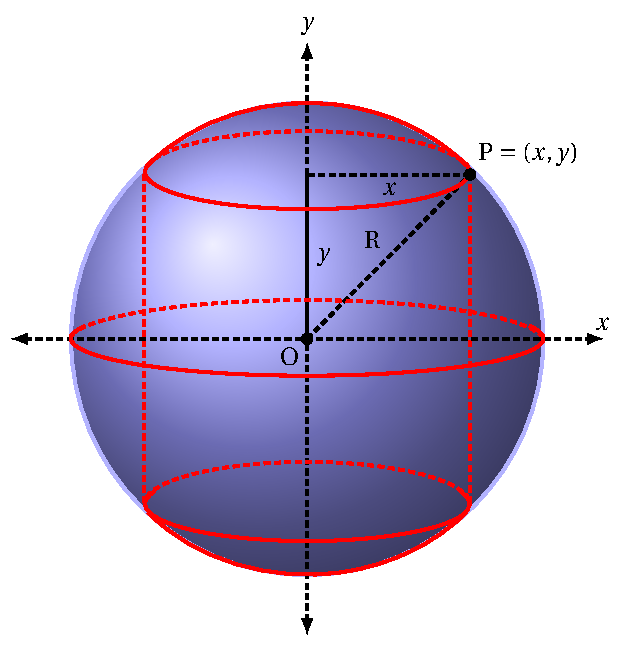
\includegraphics[scale=0.5]{65_home_antalcides_Calculo_pdf_resuelto6-9.pdf}%
\end{minipage}

\resuelto Calcula la distancia m�nima del punto $(6,3)$ a la par�bola
de ecuaci�n %
\mbox{%
$y=x^{2}$.%
}

\sol

La distancia del punto $(6,3)$ a un punto de la par�bola $(x,x^{2})$
viene dada por 
\[
\sqrt{(x-6)^{2}+(x^{2}-3)^{2}}.
\]
Como se trata de una funci�n positiva, calcularemos el punto donde
el cuadrado de la distancia alcanza su m�nimo absoluto. Sea 
\[
f(x)=(x-6)^{2}+(x^{2}-3)^{2}=45-12x-5x^{2}+x^{4}.
\]
Se trata de calcular el m�nimo absoluto de $f$ cuando $x\en\R$.
Observa que, en general, una funci�n continua en \R\ no tiene por
qu� alcanzar un m�nimo absoluto, pero $f$ es una \emph{funci�n polin�mica
de grado par con coeficiente l�der positivo}, por lo que la existencia
de un valor m�nimo absoluto de $f$ en \R\ est� garantizada de antemano,
aunque no vamos a usar este resultado.

Tenemos que $\,f\tl(x)=-12-10x+4x^{3}=2(x-2)(3+4x+2x^{2})$, que tiene
una �nica ra�z real $\,x=2$. Como para $x<2$ se tiene que $f\tl(x)<0$
y para $x>2$ es $f\tl(x)>0$, deducimos que en el punto $x=2$ la
funci�n $f$ alcanza un m�nimo absoluto en \R. Por tanto, el punto
de la par�bola $y=x^{2}$ cuya distancia al punto $(6,3)$ es m�nima
es el punto $(2,4)$.\hecho

\resuelto Una empresa tiene 100 casas para alquilar. Cuando la renta
es de 80\EURtm\ al mes, todas las casas est�n ocupadas. Por cada
4\EURtm\ de incremento de la renta una casa queda deshabitada. Cada
casa alquilada supone a la empresa un coste de 8\EURtm\ para reparaciones
diversas. �Cu�l es la renta mensual que permite obtener mayor beneficio?

\sol

Todo lo que hay que hacer es calcular la funci�n de beneficio. Sea
$80+x$ el precio del alquiler expresado en euros. Como es evidente
que no interesa bajar la renta de 80\EURtm, se considera que $x\geqslant0$.
El beneficio mensual viene dado por 
\[
f(x)=\left(100-\dfrac{x}{4}\right)(80+x-8)=7200+82x-\dfrac{x^{2}}{4}
\]
Tenemos que $f\tl(x)=82-\dfrac{x}{2}$. Deducimos f�cilmente que para
$x=164$ obtenemos al m�ximo beneficio. Es decir, cobrando un alquiler
de $244$\EURtm, lo que supone alquilar un total de $100-\dfrac{164}{4}=59$
casas y dejar sin alquilar 41, la empresa obtiene el m�ximo beneficio
$f(164)=13\textrm{.}924$\EURtm\ (as� es la econom�a capitalista$\ldots$).\hecho

\resuelto Se proyecta un jard�n en forma de sector circular de radio
$r$ y �ngulo central $\vartheta$. El �rea del jard�n ha de ser $A$
fija. �Qu� valores de $r$ y $\vartheta$ hacen m�nimo el per�metro
del jard�n?

\sol

\begin{minipage}[t]{0.65\textwidth}%
 \vspace{0pt}
 El �rea de un sector circular de amplitud $\vartheta$ medida en
radianes y radio $r$ es igual a $\dfrac{\vartheta}{2}r^{2}$, y su
longitud viene dada por $\,\vartheta\,r$. El per�metro del jard�n
es igual a $\vartheta\,r+2r$. Como debe ser $\dfrac{\vartheta}{2}r^{2}=A$,
es decir, $\vartheta=\dfrac{2A}{r^{2}}$, la funci�n cuyo m�nimo absoluto
debemos obtener es $\,f(r)=\dfrac{2A}{r}+2r$, donde $r>0$. Como
$\,f\tl(r)=-\dfrac{2A}{r^{2}}+2=2\dfrac{r^{2}-A}{r^{2}}$, se deduce
f�cilmente que en $r=\sqrt{A}$ $\,f\,$ alcanza un m�nimo absoluto.
El valor m�nimo del per�metro es igual a $4\sqrt{A}$.\hecho %
\end{minipage}%
\begin{minipage}[t]{0.3\textwidth}%
\vspace{0pt}
 \flushright\includegraphics[scale=0.5]{66_home_antalcides_Calculo_pdf_resuelto6-10.pdf}%
\end{minipage}

\resuelto Se corta un alambre de longitud $L$ formando un c�rculo
con uno de los trozos y un cuadrado con el otro. Calcular por d�nde
se debe cortar para que la suma de las �reas de las dos figuras sea
m�xima o sea m�nima.

\sol

Supongamos que partimos el alambre en dos trozos de longitud $x$
y $L-x$. Con el trozo de longitud $x$ formamos un cuadrado cuya
�rea ser� $x^{2}/16$, con el otro trozo formamos un c�rculo cuyo
radio, $r$, vendr� dado por $2\pi r=L-x$, y su area ser� $\pi r^{2}=\dfrac{(L-x)^{2}}{4\pi}$.
El problema consiste en calcular los puntos donde la funci�n $f(x)=\dfrac{x^{2}}{16}+\dfrac{(L-x)^{2}}{4\pi}$
alcanza su m�ximo y su m�nimo absolutos en el intervalo $[0,L]$.
Tenemos que 
\[
f\tl(x)=\dfrac{-4L+(4+\pi)x}{8\pi}.
\]
Deducimos, estudiando el signo de la derivada, que en el punto $x=\dfrac{4L}{4+\pi}$
hay un m�nimo absoluto.

Como la derivada tiene un �nico cero en $]0,L[$, deducimos que el
m�ximo absoluto de $f$ en $[0,L]$ tiene que alcanzarse en uno de
los extremos y, como $f(L)=0$, concluimos que el valor m�ximo de
$f$ se alcanza para $x=0$ y vale $f(0)=\dfrac{L^{2}}{4\pi}$.\hecho

\resuelto Dados dos puntos $A$ y $B$ situados en el primer cuadrante
del plano, calcula cu�l es el camino m�s corto para ir de $A$ a $B$
pasando por un punto del eje de abscisas.

\sol

\begin{minipage}[t]{0.5\textwidth}%
 \vspace{0pt}
 Podemos situar los puntos $A$ y $B$ de forma que $A=(0,r)$ y $B=(s,t)$
con $r,s,t$ positivos. La longitud del camino $APB$ viene dada por
$\,f(x)=\sqrt{x^{2}+r^{2}}+\sqrt{(s-x)^{2}+t^{2}}$. Debemos calcular
el m�nimo absoluto de $f(x)$ en el intervalo $[0,s]$. Tenemos que
\[
f\tl(x)=\frac{x-s}{\sqrt{t^{2}+(s-x)^{2}}}+\frac{x}{\sqrt{r^{2}+x^{2}}}
\]
Resolviendo $f\tl(x)=0$ obtenemos la soluci�n $\alpha=\dfrac{rs}{r+t}$.
(Si haces los c�lculos encontrar�s que $\dfrac{rs}{r-t}\,$ es tambi�n
una \emph{posible} soluci�n, pero $f\tl\left(\dfrac{rs}{r-t}\right)\neq0$). %
\end{minipage}%
\begin{minipage}[t]{0.45\textwidth}%
\vspace{0pt}
 \flushright \includegraphics[scale=0.5]{67_home_antalcides_Calculo_pdf_resuelto6-12.pdf}%
\end{minipage}

Es inmediato que $\alpha$ est� en el intervalo $[0,s]$. Por tanto,
los valores candidatos para ser m�nimo absoluto de $f$ en $[0,s]$
son $f(0)$, $f(s)$ y $f(\alpha)$. Como $f\tl(0)<0$ y $f\tl$ es
continua, se sigue que $f\tl(x)<0$ en un intervalo abierto que contiene
a $0$. En dicho intervalo abierto la funci�n $f$ es decreciente,
por lo que $f(0)$ no puede ser el valor m�nimo de $f$ en $[0,s]$.
An�logamente, como $f\tl(s)>0$ y $f\tl$ es continua, se sigue que
$f\tl(x)>0$ en un intervalo abierto que contiene a $s$, por lo que
$f(s)$ tampoco puede ser el valor m�nimo de $f$ en $[0,s]$. Por
exclusi�n, concluimos que $f(\alpha)=\sqrt{s^{2}+(r+t)^{2}}$ es el
valor m�nimo de $f$ en $[0,s]$.

\textbf{Comentario.} \ No es del todo inmediato comparar directamente
los valores $f(0)$, $f(s)$ y $f(\alpha)$ para ver cu�l de ellos
es el menor. Para salvar esta dificultad lo m�s c�modo es razonar
como lo hemos hecho.

Alternativamente, puedes calcular la derivada segunda 
\[
f\tl\!\tl(x)=\dfrac{t^{2}}{\big(t^{2}+(s-x)^{2}\big)^{3/2}}+\dfrac{r^{2}}{\big(r^{2}+x^{2}\big)^{3/2}}
\]
Como $f\tl\!\tl(x)>0$, se sigue que $f\tl$ es estrictamente creciente.
Luego si $x<\alpha$ es $f\tl(x)<0$, y si $\alpha<x$ es $f\tl(x)>0$;
de donde se deduce que $f$ tiene un m�nimo absoluto en $\alpha$.

En la figura sugiero una elegante y sencilla soluci�n geom�trica del
problema. El punto $D$ es el que proporciona el camino m�s corto
$\overline{AD}+\overline{DB}$. Cualquier otro camino $\overline{AP}+\overline{PB}$
es m�s largo porque un lado de un tri�ngulo $\overline{CB}=\overline{CD}+\overline{DB}=\overline{AD}+\overline{DB}$
es siempre m�s peque�o que la suma de los otros dos $\overline{CP}+\overline{PB}=\overline{AP}+\overline{PB}$.\hecho

\resuelto Se desea construir una ventana con forma de rect�ngulo
coronado de un semic�rculo de di�metro igual a la base del rect�ngulo.
Pondremos cristal blanco en la parte rectangular y cristal de color
en el semic�rculo. Sabiendo que el cristal coloreado deja pasar la
mitad de luz (por unidad de superficie) que el blanco, calcular las
dimensiones de la ventana para conseguir la m�xima luminosidad si
se ha de mantener un per�metro constante dado.

\sol

Sea $x$ la longitud de la base de la ventana y $h$ su altura. El
per�metro es igual a una cantidad dada, $A$; es decir, $2x+h+\pi\dfrac{x}{2}=A$.
La luminosidad viene dada por 
\[
f(x)=2xh+\pi\dfrac{x^{2}}{8}=x(A-x-\pi\dfrac{x}{2})+\pi\dfrac{x^{2}}{8}=A\,x-\dfrac{1}{8}(8+3\pi)x^{2}
\]
La derivada $f\tl(x)=A-\dfrac{1}{4}(8+3\pi)x$ se anula en $\dfrac{4A}{8+3\pi}$
y, como $f\scd(x)=-\dfrac{1}{4}(8+3\pi)<0$, concluimos que $f$ alcanza
un m�ximo absoluto en el punto $\dfrac{4A}{8+3\pi}$. Las dimensiones
de la ventana con mayor luminosidad son por tanto $x=\dfrac{4A}{8+3\pi}$,
$h=\dfrac{A(4+4\pi)}{16+6\pi}$.\hecho

\resuelto Se desea confeccionar una tienda de campa�a c�nica de un
volumen determinado. Calcular sus dimensiones para que la cantidad
de lona necesaria sea m�nima.

\sol

\begin{minipage}[t]{0.3\textwidth}%
 \vspace{0pt}
 Para hacer la tienda necesitamos cortar un sector circular de lona
como se indica en la figura. Sea $\vartheta$ la medida en radianes
del �ngulo central del sector y $x$ la medida del radio. La cantidad
de\linebreak{}
%
\end{minipage}%
\begin{minipage}[t]{0.65\textwidth}%
\vspace{-10pt}
 \flushright \includegraphics[scale=0.6]{68_home_antalcides_Calculo_pdf_resuelto6-13a.pdf}%
\end{minipage}\vspace{-2mm}

lona que necesitamos es igual al �rea del sector y viene dada por
$\dfrac{\vartheta}{2}x^{2}$ (si el volumen se expresa en m$^{3}$,
las dem�s medidas se expresar�n en metros). Sea $r$ el radio de la
base de la tienda y $h$ su altura. Nos dicen que el volumen de la
tienda debe ser igual a una cantidad prefijada, $V$, es decir, $V=\dfrac{1}{3}\pi r^{2}h$.

Nuestro problema es calcular el m�nimo absoluto de $\dfrac{\vartheta}{2}x^{2}$
sabiendo que la cantidad %
\mbox{%
$V=\dfrac{1}{3}\pi r^{2}h$%
} es conocida. Veamos que esta condici�n nos permite expresar $x$
en funci�n de $\vartheta$.

Observa que la longitud de la base de la tienda, $2\pi r$, debe ser
igual a la longitud, $\vartheta\,x$, del arco circular que abarca
el sector: $\,\vartheta\,x=2\pi r$, de donde, $r=\dfrac{\vartheta\,x}{2\pi}$.
Adem�s, es evidente que $\,x^{2}=h^{2}+r^{2}$, y deducimos que 
\[
h^{2}=x^{2}-r^{2}=x^{2}-\dfrac{\vartheta^{2}x^{2}}{4\pi^{2}}=x^{2}\left(1-\frac{\vartheta^{2}}{4\pi^{2}}\right)\longrightarrow h=\dfrac{x\sqrt{4\pi^{2}-\vartheta^{2}}}{2\pi}
\]
Por tanto 
\[
V=\frac{1}{3}\pi r^{2}h=\frac{1}{3}\pi\dfrac{\vartheta^{2}x^{2}}{4\pi^{2}}\dfrac{x\sqrt{4\pi^{2}-\vartheta^{2}}}{2\pi}=\dfrac{x^{3}\vartheta^{2}\sqrt{4\pi^{2}-\vartheta^{2}}}{24\pi^{2}}
\]
Despejando $x$, obtenemos que $\,x=\dfrac{2(3\pi^{2}V)^{1/3}}{\vartheta^{2/3}(4\pi^{2}-\vartheta^{2})^{1/6}}$.
La funci�n de la que tenemos que calcular su m�nimo absoluto es 
\[
f(\vartheta)=\frac{\vartheta}{2}x^{2}=\frac{(9\pi^{4}V^{2})^{1/3}}{\big(4\pi^{2}\vartheta-\vartheta^{3}\big)^{1/3}}\qquad(0<\vartheta<2\pi)
\]
Tenemos que $f\tl(\vartheta)=(9\pi^{4}V^{2})^{1/3}\dfrac{3\vartheta^{2}-4\pi^{2}}{3\big(4\pi^{2}\vartheta-\vartheta^{3}\big)^{4/3}}$,
que tiene un �nico cero positivo $\vartheta=\dfrac{2\pi}{\sqrt{3}}$
que corresponde, como se justifica f�cilmente estudiando el signo
de la derivada, a un m�nimo absoluto de $f$. El correspondiente valor
del radio del sector es $\,x=\sqrt[6]{\dfrac{3^{5}V^{2}}{2\pi^{2}}}$
y el �rea, $3\sqrt[6]{\dfrac{3\pi^{2}V^{4}}{4}}$.

Para un volumen $V=5\,\textrm{m}^{3}$, la cantidad de lona necesaria
es $\,\approxeq12.25\,\textrm{m}^{2}$; el radio del sector $x\approxeq2,6$m,
la altura de la tienda $h\approxeq2,12$m\, y el radio de la tienda
$r\approxeq1,5$m.\hecho

\resuelto Se desea construir un silo, con un volumen $V$ determinado,
que tenga la forma de un cilindro rematado por una semiesfera. El
costo de construcci�n (por unidad de superficie) es doble para la
semiesfera que para el cilindro (la base es gratis). Calc�lense las
dimensiones �ptimas para minimizar el costo de construcci�n.

\sol

Sea $r$ el radio de la base y $h$ la altura del cilindro. Nos dicen
que el volumen del silo, $\pi r^{2}h+\dfrac{2}{3}\pi r^{3}$, es un
valor conocido, $V$, que podemos suponer expresado en m$^{3}$. Si
el coste de construcci�n de 1\,m$^{2}$ de superficie del cilindro
es $\alpha$ euros, la funci�n de coste viene dada por $\alpha(2\pi rh)+2\alpha(2\pi r^{2})$.
De la condici�n $\,V=\pi r^{2}h+\dfrac{2}{3}\pi r^{3}$, se sigue
que $\,h=-\dfrac{2r}{3}+\dfrac{V}{\pi r^{2}}$. Sustituyendo este
valor en la funci�n de coste, resulta que la funci�n que debemos minimizar
es 
\[
f(r)=\frac{8}{3}\pi r^{2}\alpha+\frac{2V\,\alpha}{r}\qquad(r>0)
\]
Tenemos $\,f\tl(r)=\dfrac{2\alpha(8\pi r^{3}-3V)}{3r^{2}}$ que se
anula para $r=\dfrac{1}{2}\sqrt[3]{\dfrac{3V}{\pi}}$ en donde, como
se comprueba f�cilmente estudiando el signo de $f\tl(r)$, la funci�n
$f$ alcanza un m�nimo absoluto. La altura correspondiente es $h=\sqrt[3]{\dfrac{3V}{\pi}}$.
Para un volumen $V=100\,\textrm{m}^{3}$, tenemos $r\approxeq2,3\,$m
y $h\approxeq4,6\,$m.\hecho

\resuelto Demuestra que de todos los tri�ngulos is�sceles que se
pueden circunscribir a una circunferencia de radio $r$, el de �rea
m�nima es el equil�tero de altura $3r$.

\sol

\begin{minipage}[t]{0.5\textwidth}%
 \vspace{0pt}
 Sea $\alpha$ la medida en radianes de los �ngulos $\angle\,CAB=\angle\,ABC$.
El tri�ngulo $\triangle ONC$ es rect�ngulo y $\angle CON=\angle\,ABC$
por ser �ngulos con lados perpendiculares. Obtenemos as� que $\cos(\alpha)=\dfrac{r}{\overline{OC}}$,
esto es, $\overline{OC}=\dfrac{r}{\cos{\alpha}}$. Considerando el
tri�ngulo rect�ngulo $\triangle OMB$, obtenemos $\tg(\alpha/2)=\dfrac{\overline{OM}}{\overline{MB}}=\dfrac{r}{\overline{MB}}$,
de donde $\overline{MB}=r\,\cotg(\alpha/2)$. El �rea del tri�ngulo
viene dada por $\overline{MB}(\overline{OC}+r)\,$ y, sustituyendo
los valores anteriores, resulta la funci�n 
\[
f(\alpha)=r^{2}\cotg(\alpha/2)\frac{1+\cos{\alpha}}{\cos\alpha}\ \ensuremath{0<\alpha<\pi/2)}
\]
%
\end{minipage}%
\begin{minipage}[t]{0.45\textwidth}%
\vspace{-10pt}
 \flushright\includegraphics[scale=0.7]{69_home_antalcides_Calculo_pdf_resuelto6-14.pdf}%
\end{minipage}

Como 
\[
f\tl(\alpha)=r^{2}\dfrac{(1-2\cos\alpha)\cos^{2}(\alpha/2)}{\cos^{2}(\alpha)\sen^{2}(\alpha/2)}
\]
deducimos que la derivada tiene un �nico cero que se obtiene cuando
\mbox{%
$1-2\cos\alpha=0$,%
} lo que implica que $\alpha=\pi/3$. Se comprueba f�cilmente, estudiando
el signo de la derivada, que dicho valor corresponde a un m�nimo absoluto
del �rea. Por tanto, de todos los tri�ngulos is�sceles que se pueden
circunscribir a una circunferencia de radio $r$, el de �rea m�nima
es el equil�tero; su altura es igual a $\,\overline{OC}+r=\dfrac{r}{\cos{\alpha}}+r=2r+r=3r\,$
y su �rea vale $3r^{2}\sqrt{3}$.\hecho

\resuelto Con una cuerda de longitud $L$, con un nudo corredizo
en uno de sus extremos, rodeamos una columna circular de radio $R$
haciendo pasar el otro extremo por el nudo. Calcula la m�xima distancia
posible del extremo libre al centro de la columna.

\sol

\begin{minipage}[t]{0.5\textwidth}%
 \vspace{0pt}
 Para hacer este ejercicio debes tener en cuenta que en los puntos
donde la cuerda se separa de la columna lo hace en la direcci�n de
la tangente a la circunferencia. En la figura se han representado
los radios $\overline{OC}$ y $\overline{OB}$ que unen el centro
de la circunferencia con los puntos de tangencia. Lo que nos piden
es calcular la longitud m�xima del segmento $\overline{OP}$ conociendo
la\linebreak{}
%
\end{minipage}%
\begin{minipage}[t]{0.45\textwidth}%
\vspace{-5pt}
 \hspace{1cm} \includegraphics[scale=0.7]{70_home_antalcides_Calculo_pdf_resuelto6-15.pdf}%
\end{minipage}\vspace{4mm}

longitud de la cuerda y el radio de la columna. Tenemos que $\overline{OP}=\overline{OA}+\overline{AP}$,
como el tri�ngulo $\triangle OCA$ es rect�ngulo, se verifica que
$\overline{OA}=\dfrac{R}{\sen\vartheta}$, donde $\vartheta$ es la
medida en radianes del �ngulo $\angle OAC$.

La longitud del arco de circunferencia desde $C$ hasta $B$ en sentido
contrario a las agujas del reloj, es igual a $\,R(\pi+2\vartheta)$;
adem�s se verifica que $\tg\vartheta=\dfrac{\overline{OC}}{\overline{AC}}=\dfrac{R}{\overline{AC}}$.
Deducimos as� que 
\[
\overline{AP}=L-2\overline{AC}-CB{\raisebox{2.5mm}{\hspace{-4mm}{\ensuremath{\frown}}}}=L-2R\dfrac{\cos\vartheta}{\sen\vartheta}-R(\pi+2\vartheta)
\]
Por tanto 
\[
f(\vartheta)=\dfrac{R}{\sen\vartheta}+L-2R\dfrac{\cos\vartheta}{\sen\vartheta}-R(\pi+2\vartheta)\qquad0<\vartheta\leqslant\pi/2
\]
es la funci�n que nos da la longitud del segmento $\overline{OP}$.
Calculando su derivada y simplificando resulta 
\[
f\tl(\vartheta)=R\dfrac{\cos\vartheta(2\cos\vartheta-1)}{\sen^{2}\vartheta}.
\]
La derivada se anula solamente cuando $2\cos\vartheta-1=0$, es decir,
$\vartheta=\pi/3$. Se comprueba f�cilmente, por ejemplo estudiando
el signo de $f\tl(\vartheta)$, que dicho valor corresponde a un m�ximo
absoluto de $f$ en $]0,\pi/2]$. La longitud m�xima del segmento
$\overline{OP}$ es igual a $f(\pi/3)=L-\dfrac{5\pi R}{3}$.

\textbf{Comentario.}\ Es claro que la longitud de la cuerda debe
ser suficiente para rodear la columna, es decir, $L\geqslant2\pi R$.
Pero observa que si $L=2\pi R$ no podemos separarnos de la columna.
Para que el ejercicio \emph{tenga sentido} es necesario que podamos
alejarnos m�s o menos de la columna, dependiendo de la posici�n del
nudo corredizo, y para eso es preciso que $L>2\pi R$.

F�jate tambi�n en que $\limrgt{f(\vartheta)}{\vartheta}{0}=-\infty$,
por lo que $f(\vartheta)$ toma valores negativos cuando $\vartheta$
es suficientemente peque�o. Esto nos dice que la funci�n $f(\vartheta)$
no siempre representa la longitud del segmento $\overline{OP}$. De
hecho, como $\sen\vartheta=\dfrac{R}{\overline{OA}}$ y $\overline{OA}\leqslant L+R$,
se sigue que $\sen\vartheta\geqslant\dfrac{R}{L+R}$, lo que implica
que $\vartheta\geqslant\vartheta_{0}$ donde $\vartheta_{0}=\arcsen\left(\dfrac{R}{L+R}\right)$.
Estas consideraciones no afectan a la soluci�n obtenida porque hemos
calculado el m�ximo absoluto de $f$ en \emph{todo} el intervalo $]0,\pi/2]$,
salvo por un detalle: debemos asegurarnos de que es posible separar
el nudo de la columna hasta que $\vartheta\leqslant\pi/3$. Para eso
\emph{es suficiente que la longitud de la cuerda sea mayor o igual}
que $R(\pi+2\pi/3)+2R/\sqrt{3}$ (la longitud del arco $CB{\raisebox{2.5mm}{\hspace{-4mm}{\ensuremath{\frown}}}}$
m�s dos veces la longitud del segmento $\overline{AC}$ correspondientes
a $\vartheta=\pi/3$). Observa que $R(\pi+2\pi/3)+2R/\sqrt{3}=\dfrac{2\sqrt{3}R+5\pi R}{3}>2\pi R$.\hecho

\resuelto El principio de Fermat afirma que la luz viaja de un punto
$A$ a otro punto $B$ siguiendo la trayectoria en la que se invierte
el menor tiempo posible. Supongamos que el eje de abscisas, $y=0$,
separa dos medios en los que la luz viaja a distinta velocidad (por
ejemplo, aire y agua). Sea $c$ la velocidad de la luz en el semiplano
superior $y>0$ y sea $\frac{3}{4}c$ la velocidad en el semiplano
inferior $y<0$. Calcula el punto del eje de abscisas por el que pasar�
el rayo que viaje desde el punto $A=(-4,3)$ al $B=(3,-4)$.

\sol

\begin{minipage}[t]{0.5\textwidth}%
 \vspace{0pt}
 Se trata de calcular $P=(x,0)$ por la condici�n de que el tiempo
total invertido por el rayo de luz para recorrer el camino $\overline{APB}$
sea m�nimo. Sea $t_{1}$ el tiempo que tarda la luz en recorrer el
segmento $\overline{AP}$ y $t_{2}$ el tiempo que tarda la luz en
recorrer el segmento $\overline{PB}$. Tenemos que: 
\[
\begin{split}\textrm{longitud}(\overline{AP}) & =\sqrt{(x+4)^{2}+9}=c\,t_{1}\\
\textrm{longitud}(\overline{PB}) & =\sqrt{(x-3)^{2}+16}=\frac{3}{4}c\,t_{2}
\end{split}
\]
%
\end{minipage}%
\begin{minipage}[t]{0.45\textwidth}%
\vspace{-10pt}
 \flushright \includegraphics[scale=0.6]{71_home_antalcides_Calculo_pdf_resuelto6-16.pdf}%
\end{minipage}\vspace{0.5cm}

La funci{�}n cuyo m�nimo debemos calcular es 
\[
f(x)=t_{1}+t_{2}=\dfrac{\sqrt{(x+4)^{2}+9}}{c}+\dfrac{4\sqrt{(x-3)^{2}+16}}{3c}
\]
Cuya derivada es 
\[
f\tl(x)=\dfrac{1}{3c}\dfrac{3(x+4)}{\sqrt{(x+4)^{2}+9}}+\dfrac{1}{3c}\dfrac{4(x-3)}{\sqrt{(x-3)^{2}+16}}
\]
Es claro que $x=0$ es un cero de la derivada. Veamos si corresponde
a un m�nimo absoluto de $f(x)$. Calculando la derivada segunda y
simplificando obtenemos que 
\[
f\scd(x)=\dfrac{1}{3c}\dfrac{27}{\sqrt{((x+4)^{2}+9)^{3}}}+\dfrac{1}{3c}\dfrac{64}{\sqrt{((x-3)^{2}+16)^{3}}}
\]
Resulta as� que $f\scd(x)>0$ para todo $x$ por lo que la derivada
$f\tl$ es estrictamente creciente y, al ser $f\tl(0)=0$, se sigue
que $f\tl(x)<0$ para $x<0$ y $f\tl(x)>0$ para $x>0$, luego $f$
es decreciente en $]-\infty,0]$ y creciente en $[0,+\infty[$ y,
en consecuencia, $f$ tiene un m�nimo absoluto en $x=0$.\hecho

\resuelto Calcula la posici�n del punto $P=(x,0)$ en la figura de
la derecha, donde $A=(0,1)$ y $B=(2+\sqrt{3},2)$, para que el �ngulo
$\theta$ sea m�ximo. �Cu�l es dicho valor m�ximo de $\theta$? Justifica
con detalle lo que haces.

\sol

\begin{minipage}[t]{0.5\textwidth}%
 \vspace{0pt}
 Tenemos que $\dis\theta=\pi-\theta_{1}-\theta_{2}$, es decir\linebreak{}
$\theta=(\frac{\pi}{2}-\theta_{1})+(\frac{\pi}{2}-\theta_{2})=\beta_{1}+\beta_{2}$
y deducimos f�cilmente que 
\[
\theta(x)=\arctg x+\arctg\left(\dfrac{2+\sqrt{3}-x}{2}\right)
\]
Derivando, tenemos 
\[
\theta\tl(x)=\dfrac{1}{1+x^{2}}+\dfrac{-1/2}{1+\left(\dfrac{2+\sqrt{3}-x}{2}\right)^{2}}
\]
%
\end{minipage}%
\begin{minipage}[t]{0.45\textwidth}%
\vspace{1pt}
 \flushright\includegraphics[scale=0.45]{72_home_antalcides_Calculo_pdf_resuelto6-17.pdf}%
\end{minipage}

Simplificando resulta 
\[
\theta\tl(x)=\dfrac{9+4\sqrt{3}-(4+2\sqrt{3})x-x^{2}}{(1+x^{2})(4+(2+\sqrt{3}-x)^{2})}
\]
Los ceros de la derivada son las ra�ces de $\ x^{2}+(4+2\sqrt{3})x-4\sqrt{3}-9=0$,
que vienen dadas por 
\[
\alpha=\dfrac{-4-2\sqrt{3}+\sqrt{(4+2\sqrt{3})^{2}+4(4\sqrt{3}+9)}}{2},\quad\beta=\dfrac{-4-2\sqrt{3}-\sqrt{(4+2\sqrt{3})^{2}+4(4\sqrt{3}+9)}}{2}
\]
 Como $(4+2\sqrt{3})^{2}+4(4\sqrt{3}+9)=32(2-\sqrt{3})=16(4+2\sqrt{3})=16(\sqrt{3}+1)^{2}$.
Naturalmente, como $0\leqslant x\leqslant2+\sqrt{3}$, y $\beta<0$
se sigue que 
\[
\alpha=\dfrac{-4-2\sqrt{3}+\sqrt{16(\sqrt{3}+1)^{2}}}{2}=\sqrt{3}
\]
es el �nico cero de la derivada en el intervalo $[0,2+\sqrt{3}]$.

Estudiemos ahora el signo de la derivada. Como el denominador de $\theta\tl(x)$
es positivo, el signo de $\theta\tl(x)$ es igual al de $9+4\sqrt{3}-(4+2\sqrt{3})x-x^{2}$.
Pero 
\[
9+4\sqrt{3}-(4+2\sqrt{3})x-x^{2}=-(x-\alpha)(x-\beta)
\]
que es positivo cuando $\beta<x<\alpha$ y negativo si $x<\beta$
o $\alpha<x$. Deducimos que $\theta\tl(x)>0$ si $0\leqslant x<\sqrt{3}$
y $\theta\tl(x)<0$ si $\sqrt{3}<x\leqslant2+\sqrt{3}$. Por tanto,
la funci�n $\theta$ es creciente en $[0,\sqrt{3}]$ y decreciente
en $[\sqrt{3},2+\sqrt{3}]$. Concluimos que en $\sqrt{3}$ la funci�n
$\theta$ alcanza un m�ximo absoluto en $[0,2+\sqrt{3}]$. El valor
m�ximo es $\theta(\sqrt{3})=\arctg(\sqrt{3})+\arctg(1)=\pi/3+\pi/4=7\pi/12$.\hecho

\resuelto Calcula el l�mite en el punto $a$ que en cada caso se
indica de las siguientes funciones: 
\[
\begin{array}{ll}
\dis f(x)=(\sen x+\cos x)^{1/x},\ \ a=0; & \dis f(x)=(1+\tg x)^{1/x^{2}},\ \ a=0\\
\dis f(x)=(\cot x)^{\sen\,x},\ \ a=0,\,\pi/2; & \dis f(x)=\left(\cos\!^{2}x+\frac{x^{2}}{2}\right)^{1/x^{2}},\ \ a=0\\
\rule{0mm}{7mm}\dis f(x)=(1+\sen x)^{\cotg x},\ \ a=0,\,\pi/2; & \dis f(x)=\frac{\log(\sen x)}{(\pi-2x)^{2}},\ \ a=\pi/2\\
\rule{0mm}{7mm}\dis f(x)=\frac{x-\arctg x}{\sen\!^{3}x},\ \ a=0; & \dis f(x)=\frac{(\tg x)(\arctg x)-x^{2}}{x^{6}},\ \ a=0\\
\rule{0mm}{7mm}\dis f(x)=\dfrac{\e^{x}-\cos\sqrt{2}\,x-x}{\tg\!^{2}x},\ \ a=0; & \dis f(x)=\left(\frac{\sen x}{x}\right)^{1/(1-\cos x)},\ \ a=0
\end{array}
\]
\sol

$\bullet\quad$ El l�mite \Lim{(\sen x+\cos x){1/x}}{x}{0}\ es
de la forma \Lim{f(x){g(x)}}{x}{a}\ cuando $\Lim{f(x)}{x}{a}=1$\ y
$\Lim{|g(x)|}{x}{a}=+\infty$. Se trata, por tanto, de una indeterminaci�n
del tipo $1^{\infty}$. Estos l�mites suelen poderse calcular haciendo
uso del criterio de equivalencia logar�tmica (teorema \ref{zapato})
que, en las condiciones anteriores para $f$ y $g$, nos dice que:
\[
\begin{array}{ccc}
\Lim{f(x)^{g(x)}}{x}{a}=\e^{L} & \Longleftrightarrow & \Lim{g(x)(f(x)-1)}{x}{a}=L\\
\Lim{f(x)^{g(x)}}{x}{a}=0 & \Longleftrightarrow & \Lim{g(x)(f(x)-1)}{x}{a}=-\infty\\
\Lim{f(x)^{g(x)}}{x}{a}=+\infty & \Longleftrightarrow & \Lim{g(x)(f(x)-1)}{x}{a}=+\infty
\end{array}
\]
En nuestro caso: 
\[
\Lim{\dfrac{1}{x}(\sen x+\cos x-1)}{x}{0}=\Lim{\dfrac{\sen x+\cos x-1}{x}}{x}{0}=\Lim{\dfrac{\sen x}{x}}{x}{0}+\Lim{\dfrac{\cos x-1}{x}}{x}{0}=1.
\]
Donde hemos usado que 
\begin{eqnarray*}
%\nonumbertoremovenumbering(beforeeachequation)
\Lim{\frac{\sen x}{x}}{x}{0} & = & \Lim{\frac{\sen x-\sen0}{x-0}}{x}{0}=\cos0=1\\
\Lim{\frac{\cos x-1}{x}}{x}{0} & = & \Lim{\frac{\cos x-\cos0}{x-0}}{x}{0}=\sen0=0
\end{eqnarray*}
sin m�s que recordar la definici�n de derivada de una funci�n en un
punto. Concluimos as� que 
\[
\Lim{(\sen x+\cos x)^{1/x}}{x}{0}=\e
\]

$\bullet\quad$ El l�mite \Lim{(1+\tg x){1/x{2}}}{x}{0}\ es
del mismo tipo anterior. Ahora, el l�mite 
\[
\Lim{\dfrac{\tg x}{x^{2}}}{x}{0}=\Lim{\dfrac{\sen x}{x}\dfrac{1}{x\cos x}}{x}{0}
\]
no existe, pues 
\[
\limrgt{\dfrac{1}{x\cos x}}{x}{0}=+\infty,\quad\limlft{\dfrac{1}{x\cos x}}{x}{0}=-\infty.
\]
Luego $\limrgt{(1+\tg x)^{1/x^{2}}}{x}{0}=+\infty$ y %
\mbox{%
$\limlft{(1+\tg x)^{1/x^{2}}}{x}{0}=0$.%
}

$\bullet\quad$ El l�mite \Lim{\left(\cos{2}x+\frac{x2}{2}\right){1/x{2}}}{x}{0}\ es
del mismo tipo que los anteriores. Tenemos ahora que: 
\[
\Lim{\dfrac{\cos^{2}x+x^{2}/2-1}{x^{2}}}{x}{0}=\Lim{\dfrac{-\sen^{2}x+x^{2}/2}{x^{2}}}{x}{0}=-\Lim{\left(\dfrac{\sen x}{x}\right)^{2}}{x}{0}+\dfrac{1}{2}=-\frac{1}{2}
\]
Luego, $\Lim{\left(\cos^{2}x+\frac{x^{2}}{2}\right)^{1/x^{2}}}{x}{0}=\dfrac{1}{\sqrt{\e}}$.

$\bullet\quad$ El l�mite \Lim{\left(\frac {\sen x}{x}\right){1/(1-\cos
x)}}{x}{0}\ es del mismo tipo que los anteriores. Tenemos ahora
que 
\[
\Lim{\left(\frac{\sen x}{x}-1\right)\frac{1}{1-\cos x}}{x}{0}=\Lim{\frac{\sen x-x}{x(1-\cos x)}}{x}{0}
\]
Este �ltimo l�mite no tiene dificultad y puede hacerse por L'H�pital.
Pero es m�s f�cil usar los l�mites ``bien conocidos'': 
\[
\frac{\sen x-x}{x(1-\cos x)}=\frac{\sen x-x}{x^{3}}\frac{x^{2}}{1-\cos x}.
\]
Deducimos que \Lim{\frac{\sen x - x}{x(1-\cos x)}}{x}{0}$=\dfrac{-1}{3}$.
Luego $\Lim{\left(\frac{\sen x}{x}\right)^{1/(1-\cos x)}}{x}{0}=\dfrac{1}{\sqrt[3]{\e}}$.

$\bullet\quad$ El l�mite \Lim{\dfrac{\e{x}-\cos \sqrt{2\,}x
- x}{\tg\!{2}x}}{x}{0}\ es una indeterminaci�n del tipo
$\dfrac{0}{0}$ y puede hacerse por L'H�pital, pero antes es conveniente
sustituir $\tg x$ por $x$ pues son funciones asint�ticamente equivalentes
para $x\to0$. Escribiendo: 
\[
\dfrac{\e^{x}-\cos\sqrt{2}\,x-x}{\tg\!^{2}x}=\frac{x^{2}}{\tg\!^{2}x}\frac{\e^{x}-\cos\sqrt{2}\,x-x}{x^{2}}
\]
y teniendo en cuenta que $\Lim{\left(\frac{x}{\tg x}\right)^{2}}{x}{0}=1$,
basta calcular \Lim{\dfrac{\e{x}-\cos \sqrt{2}\,x - x}{x{2}}}{x}{0}\ lo
que puedes hacer por L'H�pital muy f�cilmente.

$\bullet\quad$ El l�mite \Lim{\frac{\log (\sen x)}{(\pi
-2x){2}}}{x}{\pi/2}\ es tambi�n una indeterminaci�n del
tipo $\dfrac{0}{0}$ y, en principio, puede hacerse por L'H�pital.
Hazlo t� aplicando L'H�pital. Yo voy a reducirlo a l�mites ``bien
conocidos''.

Lo primero que voy a hacer es convertir el l�mite para $x\to\pi/2$
en un l�mite para $x\to0$. Para ello basta sustituir $x$ po $\pi/2-x$
como sigue: 
\[
\Lim{\frac{\log(\sen x)}{(\pi-2x)^{2}}}{x}{\pi/2}=\Lim{\frac{\log(\sen(\pi/2-x))}{(\pi-2(\pi/2-x))^{2}}}{x}{0}=\Lim{\frac{\log(\cos x)}{4x^{2}}}{x}{0}
\]
Ahora, la presencia de $x^{2}$ y de $\cos x$ me sugiere escribir
$\dfrac{\log(\cos x)}{4x^{2}}=\dfrac{\log(\cos x)}{\cos x-1}\dfrac{\cos x-1}{x^{2}}$.
El l�mite $\Lim{\dfrac{\cos x-1}{x^{2}}}{x}{0}=-1/2$ porque es uno
de los l�mites ``bien conocidos''. El l�mite $\Lim{\dfrac{\log(\cos x)}{\cos x-1}}{x}{0}=1$\ porque
tambi�n es uno de los l�mites ``bien conocidos'', pues es de la
forma \Lim{\dfrac{\log t}{t-1}}{t}{1}\ donde se ha sustituido
$t$ por $\cos x$.

Por tanto $\Lim{\dfrac{\log(\sen x)}{(\pi-2x)^{2}}}{x}{\pi/2}=-\dfrac{1}{2}$.

Los restantes l�mites de este ejercicio te los dejo para que los hagas
t�.\hecho

\resuelto Justifica que para todo $r\en\R$ y para todo $s>0$ se
verifica que: 
\[
\Lim{\dfrac{(\log x)^{r}}{x^{s}}}{x}{+\infty}=0,\quad\Lim{\dfrac{x^{r}}{\e^{sx}}}{x}{+\infty}=0,\quad\limrgt{x^{s}\vert\log x\vert^{r}}{x}{0}=0.
\]

\sol

Es suficiente probar que para todo $n\en\N$ se verifica $\Lim{\dfrac{(\log x)^{n}}{x^{s}}}{x}{+\infty}=0$.
Podemos hacerlo por inducci�n. Para $n=1$, tenemos, aplicando L'H�pital
por tratarse de una indeterminaci�n $\frac{\infty}{\infty}$, que:
\[
\Lim{\dfrac{\log x}{x^{s}}}{x}{+\infty}=\frac{1}{s}\Lim{\dfrac{1}{x^{s}}}{x}{+\infty}=0.
\]
Supuesto demostrado que $\Lim{\dfrac{(\log x)^{n}}{x^{s}}}{x}{+\infty}=0$,
tenemos: 
\[
\Lim{\dfrac{(\log x)^{n+1}}{x^{s}}}{x}{+\infty}=\frac{n+1}{s}\Lim{\dfrac{(\log x)^{n}}{x^{s}}}{x}{+\infty}=0.
\]
Lo que concluye la demostraci�n por inducci�n.

Haciendo la sustituci�n de $x$ por $\e^{x}$ en el l�mite anterior,
obtenemos: 
\[
0=\Lim{\dfrac{(\log x)^{r}}{x^{s}}}{x}{+\infty}=[x\leftrightarrow\e^{x}]=\Lim{\dfrac{x^{r}}{\e^{sx}}}{x}{+\infty}
\]
Haciendo la sustituci�n de $x$ por $1/x$ en el l�mite primero, obtenemos:
\[
0=\Lim{\dfrac{(\log x)^{r}}{x^{s}}}{x}{+\infty}=[x\leftrightarrow1/x]=\limrgt{x^{s}\vert\log x\vert^{r}}{x}{0}
\]
\hecho

\resuelto Calcula el l�mite en el punto $a$ que en cada caso se
indica de las funciones $\,f:\R^{+}\rightarrow\R$. 
\[
f(x)=\frac{x^{2}\sen1/x}{\log x},\ \ a=+\infinity;\qquad f(x)=\sen\sqrt{1+x}-\sen\sqrt{x},\ \ a=+\infinity
\]
\[
f(x)=\sen x\,\sen\frac{1}{x},\ \ a=0,\ a=+\infinity;\qquad f(x)=\left(\cos\frac{\pi}{x+2}\right)^{x^{2}},\ \ a=+\infinity
\]

\sol

El l�mite \Lim{\dfrac{x{2}\sen 1/x}{\log x}}{x}{+\infty}\ es,
de hecho, una indeterminaci�n del tipo $\frac{\infty}{\infty}$ y
puedes intentar hacerlo por L'H�pital. Prueba a ver qu� pasa. En este
caso el marqu�s de L'H�pital no resuelve el l�mite. Pero es f�cil
ver que $\Lim{x\sen(1/x)\dfrac{x}{\log x}}{x}{+\infty}=+\infty$,
porque $\Lim{x\sen(1/x)}{x}{+\infty}=\limrgt{\dfrac{\sen x}{x}}{x}{0}=1$
y $\Lim{\dfrac{x}{\log x}}{x}{+\infty}=+\infty$.

El l�mite \Lim{\big(\sen \sqrt{1+x} - \sen \sqrt{x}\big)}{x}{+\infty}\ no
entra dentro de ninguna de las indeterminaciones usuales. De hecho,
el l�mite $\Lim{\sen\sqrt{x}}{x}{+\infty}$ no existe (�sabes probarlo?).
Est� claro que el l�mite que nos piden calcular requiere un tratamiento
particular. Despu�s de pensarlo un poco, a la vista de c�mo es la
funci�n, se me ocurre usar el teorema del valor medio. Dicho teorema,
aplicado a la funci�n $\sen\sqrt{x}$ en el intervalo $[x,x+1]$,
me dice que hay alg�n punto $z\in]x,x+1[$ tal que $\sen\sqrt{x+1}-\sen\sqrt{x}=\dfrac{\cos z}{2\sqrt{z}}$,
y tomando valores absolutos deducimos 
\[
\modulo{\sen\sqrt{x+1}-\sen\sqrt{x}}=\left\vert \dfrac{\cos z}{2\sqrt{z}}\right\vert \leqslant\dfrac{1}{2\sqrt{x}}
\]
de donde se deduce que $\Lim{\big(\sen\sqrt{1+x}-\sen\sqrt{x}\big)}{x}{+\infty}=0$.

El l�mite \Lim{\left (\cos \frac{\pi}{x+2} \right ){x2}}{x}{+\infty}\ es
una indeterminaci�n $1^{\infty}$ y aplicaremos el criterio de equivalencia
logar�tmica. Para ello, calculamos 
\begin{align*}
\Lim{x^{2}\left(\cos\left(\frac{\pi}{x+2}\right)-1\right)}{x}{+\infty} & =\limrgt{\dfrac{\cos\left(\dfrac{\pi x}{1+2x}\right)-1}{x^{2}}}{x}{0}=\\
 & =\limrgt{\dfrac{\ \cos\left(\dfrac{\pi\,x}{1+2x}\right)-1\ }{\left(\dfrac{\pi x}{1+2x}\right)^{2}}\ \dfrac{\left(\dfrac{\pi\,x}{1+2x}\right)^{2}}{x^{2}}}{x}{0}=\frac{-\pi^{2}}{2}
\end{align*}
Luego $\Lim{\left(\cos\frac{\pi}{x+2}\right)^{x^{2}}}{x}{+\infty}=\e^{-\pi^{2}/2}$.
El l�mite que queda por hacer es inmediato. \hecho

\resuelto Sea \func{g}{\R}\ derivable en \R\ y dos veces
derivable en 0 siendo, adem�s, $g(0)=0$. Definamos \func{f}{\R}\ por
$f(x)=\dfrac{g(x)}{x}$\ si $\,x\neq0$ y $f(0)=g\tl(0)$. Estudia
la derivabilidad de $f$. �Es $f\tl$ continua en 0?

\sol Por la regla de la cadena, $f$ es derivable en todo punto $x\neq0$
y, por la regla de derivaci�n de un cociente, tenemos que $\,f\tl(x)=\dfrac{x\,g\tl(x)-g(x)}{x^{2}}$
para $x\neq0$. Para estudiar si $f$ es derivable en $x=0$ no hay
otra forma de hacerlo (pero lee m�s abajo) que recurriendo a la definici�n.
Tenemos que 
\[
\Lim{\dfrac{f(x)-f(0)}{x-0}}{x}{0}=\Lim{\dfrac{g(x)-g\tl(0)x}{x^{2}}}{x}{0}=\dfrac{g\tl\!\tl(0)}{2}
\]
en virtud del teorema de Taylor-Young (si lo prefieres, puedes aplicar
-�una vez solo!- L'H�pital). Por tanto, $f$ es derivable en $x=0$
y $f\tl(0)=\dfrac{g\tl\!\tl(0)}{2}$.

Estudiemos si $f\tl$ es continua en $x=0$. Tenemos que $\Lim{f\tl(x)}{x}{0}=\Lim{\dfrac{x\,g\tl(x)-g(x)}{x^{2}}}{x}{0}$
y para calcular este l�mite \emph{no} se puede aplicar L'H�pital porque
no sabemos si $g\tl$ es derivable (nos dicen que $g$ es \emph{una}
vez derivable en \R). Intentaremos relacionar el cociente con las
hip�tesis que nos dan sobre $g$. Despu�s de pensarlo un poco, parece
conveniente escribir: 
\[
\dfrac{x\,g\tl(x)-g(x)}{x^{2}}=\dfrac{x\,g\tl(x)-x\,g\tl(0)+x\,g\tl(0)-g(x)}{x^{2}}=\dfrac{g\tl(x)-g\tl(0)}{x}-\dfrac{g(x)-g\tl(0)x}{x^{2}}
\]
y deducimos que $\Lim{f\tl(x)}{x}{0}=\dfrac{g\tl\!\tl(0)}{2}$, luego
$f\tl$ es continua en $x=0$.

Tambi�n puedes usar para hacer este ejercicio un resultado de teor�a
que dice que si una funci�n $f$ es continua en un intervalo $I$,
$a$ es un punto de $I$, y sabemos que $f$ es derivable en $I\setminus\{a\}$
y que $\Lim{f\tl(x)}{x}{a}=L$, entonces $f$ tambi�n es derivable
en $a$ con $f\tl(a)=L\,$ y, por tanto, $f\tl$ es continua en $a$.

Es evidente (�o no lo es?) que la funci�n $f$ del ejercicio es continua
en el intervalo $I=\R$ y es derivable en $\R\setminus\{0\}$. Como
$\Lim{f\tl(x)}{x}{0}=\dfrac{g\tl\!\tl(0)}{2}$, esto prueba de golpe
que $f$ es derivable en $x=0$, que $f\tl(0)=\dfrac{g\tl\!\tl(0)}{2}\,$
y que $f\tl$ es continua en $x=0$.\hecho

\resuelto Sean \func{f,g}{{]}-1,+\infty{[}}\ las funciones
definidas por 
\[
f(x)=\frac{\log(1+x)}{x},\ \ f(0)=1;\quad g(x)=\e^{f(x)}
\]
Calcula las derivadas primera y segunda de $f$ y $g$ en $0$ y deduce
el valor del l�mite 
\[
\lim_{x\to0}\frac{(1+x)^{1/x}-\e+\dfrac{\e}{2}x}{x^{2}}
\]

\sol Observa que si $x>-1$ y $x\neq0$ es $g(x)=(1+x)^{1/x}$ y
$g(0)=\e$. Es claro tambi�n que $f(x)=\log g(x)$. El ejercicio consiste
en calcular las dos primeras derivadas de $g$ en $x=0$. Por la regla
de la cadena es suficiente para ello calcular las dos primeras derivadas
de $f$ en $x=0$. Pues entonces $g\tl(x)=\e^{f(x)}f\tl(x)$, y $g\tl\!\tl(x)=\e^{f(x)}\big((f\tl(x))^{2}+f\tl\!\tl(x)\big)$.
F�jate en que la funci�n $f$ es m�s sencilla que la $g$. De hecho,
no es inmediato calcular directamente $g\tl(0)$ porque el l�mite
\Lim{\dfrac{(1+x){1/x}-\e}{x}}{x}{0}\ se complica
un poco si tratas de hacerlo por L`H�pital. Las funciones como la
$g$, esto es, las del tipo $u(x)^{v(x)}$, tienen derivadas complicadas.

Derivar $f$ es f�cil. El l�mite $\,\Lim{\dfrac{f(x)-f(0)}{x-0}}{x}{0}=\Lim{\dfrac{\log(1+x)-x}{x^{2}}}{x}{0}=\dfrac{-1}{2}$
es bien conocido. Deducimos que $f\tl(0)=\dfrac{-1}{2}$. Ahora, para
$x\neq0$, se calcula f�cilmente, por la regla de derivaci�n de un
cociente, que $\,f\tl(x)=\dfrac{x-\log(1+x)-x\,\log(1+x)}{x^{2}(1+x)}$.
Tenemos 
\[
\dfrac{f\tl(x)-f\tl(0)}{x-0}=\dfrac{x-\log(1+x)-x\,\log(1+x)+\dfrac{1}{2}x^{2}(1+x)}{x^{3}(1+x)}
\]
Se trata de calcular el l�mite para $x\to0$ de este cociente. Lo
primero es quitar el factor $(1+x)$ del denominador (evidentemente,
$(1+x)\thicksim1$ para $x\to0$). Hecho esto, nos damos cuenta de
que se trata de comparar %
\mbox{%
$x-\log(1+x)-x\,\log(1+x)+\dfrac{1}{2}x^{2}+\dfrac{1}{2}x^{3}$%
} con $x^{3}$. Utilizando el teorema de Taylor-Young (o, simplemente,
recordando los polinomios de Taylor de $\log(1+x)$ en $x=0$), tenemos
que: 
\[
\log(1+x)=x-\dfrac{1}{2}x^{2}+\dfrac{1}{3}x^{3}+o(x^{3}).
\]
Deducimos que: 
\[
x-\log(1+x)-x\,\log(1+x)+\dfrac{1}{2}x^{2}+\dfrac{1}{2}x^{3}=\dfrac{2}{3}x^{3}+o(x^{3})
\]
por lo que $\Lim{\dfrac{f\tl(x)-f\tl(0)}{x-0}}{x}{0}=\dfrac{2}{3}$,
es decir, $f\scd(0)=\dfrac{2}{3}$.

Resulta as� que $g\tl(0)=\e^{f(0)}f\tl(0)=-\dfrac{\e}{2}$ y 
\[
g\scd(0)=\e^{f(0)}\big((f\tl(0))^{2}+f\tl\!\tl(0)\big)=\e\left(\dfrac{1}{4}+\dfrac{2}{3}\right)=\dfrac{11}{12}\e.
\]

Finalmente, como consecuencia del teorema de Taylor-Young, tenemos
que: 
\[
\lim_{x\to0}\frac{(1+x)^{1/x}-\e+\dfrac{\e}{2}x}{x^{2}}=\dfrac{11}{24}\e.
\]
Porque dicho l�mite es de la forma $\Lim{\dfrac{g(x)-g(0)-g\tl(0)x}{x^{2}}}{x}{0}=\dfrac{1}{2}g\scd(0)$.\hecho

\resuelto Estudia la derivabilidad de las siguientes funciones. 
\begin{enumerate}
\item $f:\R^{+}\rightarrow\R$, dada por ${\displaystyle f(x)=x^{1/(x^{2}-1)}}$,
y $f(1)=\sqrt{\e}$. 
\item $f:]-1/2,+\infty[\rightarrow\R$, dada por ${\displaystyle f(x)=(x+\e^{x})^{1/x}}$
y $f(0)=\e^{2}$. 
\item $f:[0,+\infty[\rightarrow\R$ dada por $f(x)=(1+x\,\log x)^{1/x}$,
y $f(0)=0$. 
\item $f:\R\rightarrow\R$, dada por ${\displaystyle f(x)=\left(1+x^{2}\right)^{\sen(1/x)}}$
y $f(0)=1$. 
\item $f:]-\pi/2,\pi/2[\rightarrow\R$ dada por $f(x)=\left(\dfrac{\sen x}{x}\right)^{1/x^{2}}$
y $f(0)=\e^{-1/6}.$ 
\item \func{f}{{]}-\pi/2,\pi/2{[}}\ dada por $f(x)=\left(\dfrac{2-2\cos x}{x^{2}}\right)^{1/x}$
para $x\neq0$ y $f(0)=1$. 
\end{enumerate}
\sol En todos los casos nos piden estudiar la derivabilidad de una
funci�n de la forma %
\mbox{%
$F(x)=u(x)^{v(x)}$%
} en un punto \emph{``conflictivo''} en el que no puedes aplicar
las reglas de derivaci�n. En este tipo de ejercicios la mejor forma
de proceder consiste en estudiar la derivabilidad de la funci�n $\ff(x)=\log F(x)=v(x)\log u(x)$
en el punto conflictivo. Para ello debes recurrir a la definici�n
de derivada. Observa que como $F(x)=\e^{\ff(x)}$, la derivabilidad
de $\ff$ equivale a la derivabilidad de $F$. Como en el ejercicio
anterior ya hemos usado esta estrategia, un par de ejemplos m�s deben
ser suficiente para que la comprendas bien. Consideraremos las dos
�ltimas funciones propuestas.

5) 
\[
f(x)=\left(\frac{\sen x}{x}\right)^{1/x^{2}},\qquad f(0)=\e^{-1/6}
\]

Tenemos que $\ff(x)=\log f(x)=\dfrac{\log\left(\dfrac{\sen x}{x}\right)}{x^{2}}$,
$\ff(0)=\log f(0)=\dfrac{-1}{6}$. Tenemos: 
\[
\Lim{\dfrac{\ff(x)-\ff(0)}{x-0}}{x}{0}=\Lim{\dfrac{\log\left(\dfrac{\sen x}{x}\right)+\dfrac{1}{6}x^{2}}{x^{3}}}{x}{0}=
\]
Podemos aplicar L'H�pital para quitar el logaritmo. 
\begin{align*}
\Lim{\dfrac{\ff(x)-\ff(0)}{x-0}}{x}{0} & =\Lim{\dfrac{\dfrac{x}{\sen x}\left(\dfrac{x\,\cos x-\sen x}{x^{2}}\right)+\dfrac{1}{3}x}{3x^{2}}}{x}{0}=\\
 & =\Lim{\dfrac{x\cos x-\sen x+\dfrac{1}{3}x^{2}\sen x}{3x^{3}\sen x}}{x}{0}
\end{align*}
Sustituimos en el denominador $\sen x$ por $x$. Usando que 
\[
\sen x=x-\dfrac{1}{6}x^{3}+o(x^{4}),\quad\cos x=1-\dfrac{1}{2}x^{2}+o(x^{3})
\]
deducimos que $x\cos x-\sen x+\dfrac{1}{3}x^{2}\sen x=o(x^{4})$,
por lo que 
\[
\Lim{\dfrac{x\,\cos x-\sen x+\dfrac{1}{3}x^{2}\sen x}{3x^{4}}}{x}{0}=0
\]
Concluimos que $\ff$ es derivable en $x=0$ y $\ff\tl(0)=0$ por
lo que tambi�n $f$ es derivable en $x=0$ y $f\tl(0)=f(0)\ff\tl(0)=0$.

6) 
\[
f(x)=\left(\dfrac{2-2\cos x}{x^{2}}\right)^{1/x},\quad f(0)=1
\]

Es m�s f�cil estudiar la derivabilidad de $\ff(x)=\log f(x)$. N�tese
que al ser $f(x)=\exp(\ff(x))$, en todo punto $a$ en que sea derivable
$\ff$ tambi�n, en virtud de la regla de la cadena, ser� derivable
$f$ siendo $f\tl(a)=\ff\tl(a)\exp(\ff(a))=\ff\tl(a)f(a)$. Tenemos
que 
\[
\ff(x)=\dfrac{\log\left(\dfrac{2-2\cos x}{x^{2}}\right)}{x}
\]
para $x\neq0$, y $\ff(0)=0$. Para estudiar la derivabilidad de $\ff$
en $x=0$ consideremos el cociente: 
\[
H(x)=\frac{\ff(x)-\ff(0)}{x-0}=\frac{\log\left(\dis\frac{2-2\cos x}{x^{2}}\right)}{x^{2}}
\]
Se trata de calcular \Lim{H(x)}{x}{0}. Puesto que 
\begin{equation}
\Lim{\dis\frac{2-2\cos x}{x^{2}}}{x}{0}=1\label{limitev}
\end{equation}
el l�mite buscado es una indeterminaci�n de la forma $\frac{0}{0}$
y se dan las condiciones que permiten aplicar la regla de L'H�pital.
Tenemos entonces, supuesto que los l�mites en cuesti�n existen: 
\[
\Lim{H(x)}{x}{0}=\lim_{x\to0}\frac{x^{2}}{2-2\cos x}\frac{\dis\frac{2x^{2}\sen x-2x(2-2\cos x)}{x^{4}}}{2x}=\lim_{x\to0}\frac{x\sen x+2\cos x-2}{x^{4}}
\]
donde hemos tenido en cuenta \eqref{limitev}. Podemos volver a usar
la regla de L'H�pital para calcular el �ltimo l�mite, obteniendo:
\[
\lim_{x\to0}\frac{x\sen x+2\cos x-2}{x^{4}}=\lim_{x\to0}\frac{x\cos x-\sen x}{4x^{3}}=\lim_{x\to0}\frac{-x\sen x}{12x^{2}}=\frac{-1}{12}
\]
Hemos probado as� que $f$ es derivable en $0$ y $f\tl(0)=-1/12$.

\textbf{Comentario.}\ No debe calcularse la derivada de $f$ en $0$
aplicando la regla de L'H�pital para calcular el l�mite $\dis\lim_{x\to0}\dis\frac{f(x)-f(0)}{x-0}$,
pues entonces lo que haremos ser� calcular $\,\lim_{x\to0}f\tl(x)$.
La existencia de este l�mite, junto con la continuidad de $f$ en
$0$, implican que \emph{$f$ tiene derivada continua en $0$} y eso
es m�s de lo que se pide y, por eso mismo, suele ser m�s complicado.
\hecho

\resuelto Calcula los l�mites 
\begin{alignat*}{2}
 & 1)\ \lim_{x\to0}\left(\dfrac{1}{\sen^{2}x}-\dfrac{1}{x^{2}}\right) & \qquad & 2)\ \lim_{x\to1}\left(\dfrac{1}{\log x}-\dfrac{1}{x-1}\right)\\
 & 3)\ \lim_{x\to0}\dfrac{x\e^{2x}+x\e^{x}-2\e^{2x}+2\e^{x}}{(\e^{x}-1)^{3}} &  & 4)\ \lim_{x\to+\infty}\left(\dfrac{\pi}{2}-\arctg x\right)^{\frac{1}{\log x}}\\
 & 5)\ \lim_{x\to0}\dfrac{\log\left(\dfrac{\sen x}{x}\right)}{(\log(1+x))^{2}} &  & 6)\ \lim_{x\to0}\left(\dfrac{\tg x}{x}\right)^{1/x^{2}}\\
 & 7)\ \lim_{x\to0}\dfrac{x\log(1+\sen2x)\arctg(\sen^{3}x)}{(\e^{x}-1)(1-\cos^{2}(\tg^{2}x))} &  & 8)\ \lim_{x\to0}\dfrac{\arctg x-\sen x}{x(1-\cos x)}\\
 & 9)\ \lim_{x\to0}\dfrac{\arctg(\arcsen x^{2})}{(\e^{2x}-1)\log(1+2x)} &  & 10)\ \lim_{x\to0}\left(\frac{3\sen x-3\,x\,\cos x}{x^{3}}\right)^{1/x}
\end{alignat*}
\textbf{Sugerencia.} Pueden usarse las reglas de L'H�pital pero es
conveniente realizar previamente alguna transformaci�n.

\sol

1) Recuerda: antes de calcular un l�mite debemos simplificar todo
lo que podamos la funci�n. Tenemos que: 
\[
\dfrac{1}{\sen^{2}x}-\dfrac{1}{x^{2}}=\dfrac{x^{2}-\sen^{2}x}{x^{2}\sen^{2}x}
\]
Como $\sen x\sim x$ para $x\to0$, podemos sustituir $\sen x$ por
$x$ en el denominador (�no en el numerador!). Con ello: 
\[
\dfrac{1}{\sen^{2}x}-\dfrac{1}{x^{2}}\sim\dfrac{x^{2}-\sen^{2}x}{x^{4}}
\]
Ahora recordamos que $x-\sen x\sim x^{3}/6$ para $x\to0$, con lo
cual: 
\begin{equation}
\dfrac{x^{2}-\sen^{2}x}{x^{4}}=\dfrac{x-\sen x}{x^{3}}\dfrac{x+\sen x}{x}\label{recordar}
\end{equation}
Finalmente, deducimos que: 
\[
\lim_{x\to0}\left(\dfrac{1}{\sen^{2}x}-\dfrac{1}{x^{2}}\right)=\dfrac{1}{3}
\]
Observa que una descomposici�n como la hecha en \eqref{recordar}
solamente se te ocurre si recuerdas que $x-\sen x\sim x^{3}/6$ para
$x\to0$ (que es uno de los l�mites que debes saber de memoria). En
general, descomponer una funci�n en producto (o en suma) de otras
dos solamente debe hacerse si sabes el comportamiento de cada una
de las nuevas funciones. Hay que tener cuidado en esto porque es f�cil
equivocarse. Por ejemplo, podr�amos haber puesto: 
\[
\dfrac{x^{2}-\sen^{2}x}{x^{4}}=\dfrac{x-\sen x}{x^{2}}\dfrac{x+\sen x}{x^{2}}
\]
Con lo que introducimos una funci�n $\dfrac{x+\sen x}{x^{2}}$ que
no tiene l�mite en $0$.

2) Es muy f�cil y parecido al anterior.

3)\ Este l�mite se hace muy f�cilmente por L'H�pital pero, antes
de derivar, debes sustituir $\e^{x}-1$ por $x$.

4)\ $\dis\lim_{x\to+\infty}\left(\frac{\pi}{2}-\arctg x\right)^{\frac{1}{\log x}}$
es una indeterminaci�n tipo $0^{0}$. Sea $f(x)=\left(\dfrac{\pi}{2}-\arctg x\right)^{\frac{1}{\log x}}$.
Tomando logaritmos tenemos que $\log f(x)=\dfrac{\log\left(\dfrac{\pi}{2}-\arctg x\right)}{\log x}$.
Teniendo en cuenta que para $x>0$ es $\dfrac{\pi}{2}-\arctg x=\arctg\dfrac{1}{x}$,
se sigue que 
\[
\Lim{\log f(x)}{x}{+\infty}=\Lim{\dfrac{\log\left(\arctg\dfrac{1}{x}\right)}{-\log\dfrac{1}{x}}}{x}{+\infty}=-\limrgt{\dfrac{\log(\arctg t)}{\log t}}{t}{0}
\]
Este �ltimo l�mite puede calcularse por L'H�pital 
\[
\Lim{\log f(x)}{x}{+\infty}=-\limrgt{\dfrac{t}{(1+t^{2})\arctg t}}{t}{0}=-1
\]
Deducimos que $\Lim{f(x)}{x}{+\infty}=\dfrac{1}{\e}$.

5)\ Tambi�n puede hacerse por L'H�pital pero, antes de derivar, debes
sustituir $\log(1+x)$ por $x$. Te recuerdo que puedes sustituir
funciones asint�ticamente equivalentes en un producto o en un cociente,
nunca en una suma. Tampoco se pueden hacer estas sustituciones en
una funci�n, es decir, si $g(x)\sim h(x)$ para $x\to a$, y $F$
es una funci�n, no es cierto en general que $F(g(x))$ sea asint�ticamente
equivalente a $F(h(x))$ para $x\to a$. En este l�mite, la funci�n
$\frac{\sen x}{x}\sim1$ para $x\to0$, pero no es cierto que $\log\big(\frac{\sen x}{x}\big)\sim\log(1)=0$.

6)\ Es una indeterminaci�n $1^{\infty}$. Ya debes saberlo hacer.

7)\ Este es el t�pico l�mite en el que si aplicas directamente L'H�pital,
sin antes simplificar sustituyendo funciones por otras asint�ticamente
equivalentes, lo m�s probable es que acabes por equivocarte al derivar.
Apliquemos la primera regla: simplificar todo lo que se pueda la funci�n.

Tenemos que: 
\[
1-\cos^{2}(\tg^{2}x))=\sen^{2}(\tg^{2}x)=\left(\dfrac{\sen(\tg^{2}x)}{\tg^{2}x}\right)^{2}\tg^{4}x\sim\tg^{4}x\sim x^{4}
\]
Tambi�n es $\e^{x}-1\sim x$, $\log(1+\sen2x)\sim\sen2x\sim2x$ y
$\arctg(\sen^{3}x)\sim\sen^{3}x\sim x^{3}$. Todas estas equivalencias
asint�ticas son para $x\to0$ y todas ellas se deducen de la tabla
de los l�mites que debes saberte de memoria. En consecuencia el l�mite
que nos piden se reduce a calcular el siguiente l�mite: 
\[
\Lim{\dfrac{2x^{5}}{x^{5}}}{x}{0}=\Lim{2}{x}{0}=2
\]

Los dem�s l�mites de este ejercicio te los dejo para que los hagas
t�.\hecho

\resuelto Explica si es correcto usar las reglas de L'H�pital para
calcular los l�mites: 
\[
\lim_{x\to+\infty}\frac{x-\sen x}{x+\sen x};\qquad\lim_{x\to0}\frac{x^{2}\sen(1/x)}{\sen x}
\]

\sol Las reglas de L'H�pital dicen que, bajo ciertas hip�tesis, la
existencia de \Lim{\dfrac{f\tl(x)}{g\tl(x)}}{x}{a}\ implica
la existencia de \Lim{\dfrac{f(x)}{g(x)}}{x}{a}\ en cuyo
caso ambos l�mites coinciden. Una hip�tesis de las reglas de L'H�pital
es que la derivada del denominador no se anule en un intervalo que
tenga al punto $a$ por extremo y que el l�mite \Lim{\dfrac{f(x)}{g(x)}}{x}{a}\ sea
una indeterminaci�n.

Esto no ocurre en el caso del cociente $\,\dfrac{x-\sen x}{x+\sen x}\,$
para $x\to+\infty$ pues, aunque puede verse como una indeterminaci�n
del tipo $\dfrac{\infty}{\infty}$, la derivada del denominador es
$1+\cos x$ que se anula en todos los puntos de la forma $\pi+2k\pi$,
$k=1,2,\ldots$ por lo que \emph{no tiene sentido} considerar el l�mite
del cociente de las derivadas, \Lim{\dfrac{1-\cos x}{1+\cos
x}}{x}{+\infty}, pues dicho cociente no est� definido en ning�n
intervalo de la forma $]c,+\infty[$. Es claro, sin embargo, que:
\[
\Lim{\dfrac{x-\sen x}{x+\sen x}}{x}{+\infty}=\Lim{\dfrac{1-\dfrac{\sen x}{x}}{1+\dfrac{\sen x}{x}}}{x}{+\infty}=1
\]
En el caso del l�mite \Lim{\dfrac{x{2}\sen(1/x)}{\sen x}}{x}{0},
que puede verse como una indeterminaci�n del tipo $\dfrac{0}{0}$,
si formamos el cociente de las derivadas obtenemos la funci�n 
\[
\dfrac{2x\sen(1/x)-\cos(1/x)}{\cos x}
\]
la cual no tiene l�mite en 0 (el denominador tiene l�mite 1, pero
el numerador no tiene l�mite), luego no es posible aplicar L'H�pital
para calcular este l�mite el cual, por otra parte, es evidentemente
igual a $0$, pues: 
\[
\Lim{\dfrac{x^{2}\sen(1/x)}{\sen x}}{x}{0}=\Lim{\dfrac{x}{\sen x}\,x\sen(1/x)}{x}{0}=0
\]
\hecho

\resuelto Prueba que una funci�n polin�mica de grado $n$ coincide
con su polinomio de Taylor de orden $n$ centrado en un punto cualquiera
$a$.

\sol Las funciones polin�micas son indefinidamente derivables, por
lo que, dados $x,a\en\R$, podemos aplicar el teorema de Taylor con
resto de Lagrange para obtener que hay alg�n punto $c$ comprendido
entre $a$ y $x$ tal que: 
\[
P(x)=P(a)+P\tl(a)(x-a)+\frac{P\scd(a)}{2}(x-a)^{2}+\cdots+\frac{P^{(n)}(a)}{n!}(x-a)^{n}+\frac{P^{(n+1)}(c)}{(n+1)!}(x-a)^{n+1}
\]
Como $P$ es una funci�n polin�mica de grado $n$ su derivada de orden
$n+1$ es nula en todo punto. Luego $P^{(n+1)}(c)=0$, por lo que
resulta: 
\[
P(x)=P(a)+P\tl(a)(x-a)+\frac{P\scd(a)}{2}(x-a)^{2}+\cdots+\frac{P^{(n)}(a)}{n!}(x-a)^{n}
\]
Por tanto $P(x)$ coincide con su polinomio de Taylor de orden $n$
centrado en $a$.\hecho

\resuelto Prueba que una funci�n polin�mica $P$ tiene un cero de
orden $k$ en $a$ si, y s�lo si, puede escribirse de la forma $P(x)=(x-a)^{k}Q(x)$,
donde $Q(x)$ es una funci�n polin�mica que no se anula en $a$.

\sol Supongamos que $P(x)$ tiene un cero de orden $k$ en $a$,
es decir el valor de $P$ y el de todas sus derivadas hasta la de
orden $k-1$ son nulos en $a$ y la derivada de orden $k$ de $P$
no se anula en $a$. Entonces, como consecuencia del ejercicio anterior,
tenemos que: 
\[
P(x)=\sum_{j=0}^{n}\frac{P^{(j)}(a)}{j!}(x-a)^{j}=\sum_{j=k}^{n}\frac{P^{(j)}(a)}{j!}(x-a)^{j}=(x-a)^{k}\sum_{j=k}^{n}\frac{P^{(j)}(a)}{j!}(x-a)^{j-k}
\]
Poniendo $Q(x)=\sum_{j=k}^{n}\frac{P^{(j)}(a)}{j!}(x-a)^{j-k}$, tenemos
que $Q$ es un polinomio, $Q(a)=\frac{P^{(k)}(a)}{k!}\neq0$ y $P(x)=(x-a)^{k}Q(x)$.
El rec�proco es inmediato.\hecho

\resuelto Calcular el n�mero de ceros y la imagen de la funci�n \func{f}{\R}\ dada
por $f(x)=x^{6}-3x^{2}+2$.

\sol Se trata de un polinomio de grado par con coeficiente l�der
positivo, por tanto, alcanza un m�nimo absoluto en \R, si �ste es
igual a $m$, se tiene que $f(\R)=[m,+\infty[$. El punto (o los puntos)
en donde $f$ alcanza su m�nimo absoluto debe ser un cero de la derivada.
Como 
\[
f\tl(x)=6x^{5}-6x=6x(x^{4}-1)=6x(x^{2}-1)(x^{2}+1)=6x(x-1)(x+1)(x^{2}+1)
\]
se anula en $-1$, $0$ y $1$, se sigue que el m�nimo absoluto de
$f$ debe alcanzarse en alguno de estos puntos y, como $f(1)=f(-1)=0<f(0)$,
deducimos que $f(-1)=f(1)=0$ es el m�nimo absoluto de $f$ en \R.
Luego $f(\R)=[0,+\infty[$. Hemos determinado as� la imagen de $f$
y tambi�n hemos encontrado que $-1$ y 1 son ceros de $f$ (cosa f�cil
sin m�s que ver c�mo es $f$). Observa que $-1$ y 1 son ceros de
orden 2 de $f$ (porque son ceros simples de $f\tl$). Es claro que
$f$ no puede tener m�s ceros, porque si $f(x_{0})=0$ entonces en
$x_{0}$ la funci�n $f$ alcanza un m�nimo absoluto y, por tanto,
$f\tl$ debe anularse en $x_{0}$. En conclusi�n, $f$ tiene 4 ceros
reales (2 ceros reales dobles).\hecho

\resuelto Calcula el n�mero de soluciones de la ecuaci�n $\,3\log x-x=0$.

\sol Sea $f(x)=3\log x-x$. Observa que $\limrgt{f(x)}{x}{0}=\Lim{f(x)}{x}{+\infty}=-\infty$
y %
\mbox{%
$f(\e)=3-\e>0$.%
} Deducimos, por el teorema de Bolzano, que $f$ tiene por lo menos
un cero en cada intervalo $]0,\e[$ y $]\e,+\infty[$. Como la derivada
$f\tl(x)=\dfrac{3}{x}-1$ tiene un �nico cero en $x=3$, concluimos,
por el teorema de Rolle, que $f$ no puede tener m�s de dos ceros
distintos. En conclusi�n, la ecuaci�n $\,3\log x-x=0$ tiene una soluci�n
en el intervalo $]0,\e[$ y otra en $]\e,+\infty[$. Si quieres, puedes
precisar m�s. Como $f(1)<0$ y $f(\e^{2})=6-\e^{2}<0$, se sigue que
los dos ceros de $f$ est�n en el intervalo $]1,\e^{2}[$.\hecho

\resuelto Estudia, seg�n los valores de $\alpha$, el n�mero de ceros,
contando multiplicidades cuando proceda, de la funci�n polin�mica
$f(x)=3x^{5}+5x^{3}-30x-\alpha$. Explica con detalle lo que haces.

\sol Como consecuencia del teorema de Rolle, si la derivada de una
funci�n tiene $k$ ceros (reales) \emph{distintos} entonces la funci�n
\emph{no puede tener m�s de} $k+1$ ceros (reales) \emph{distintos}
(�pero puede que no tenga ninguno!). Sabemos tambi�n, como consecuencia
del teorema de los ceros de Bolzano, que todo polinomio de grado impar
tiene por lo menos un cero real. Como las ra�ces complejas, cuando
las hay, de polinomios con coeficientes reales, vienen por parejas
de ra�ces complejas conjugadas, deducimos que \emph{contando cada
cero tantas veces como indica su multiplicidad, todo polinomio de
grado impar y coeficientes reales tiene un n�mero impar de ceros reales}.
Por las mismas razones, \emph{contando cada cero tantas veces como
indica su multiplicidad, todo polinomio de grado par y coeficientes
reales tiene un n�mero par de ceros reales y tambi�n puede que no
tenga ninguno}.

En nuestro caso: 
\[
f\tl(x)=15x^{4}+15x^{2}-30=15(x^{2}+2)(x^{2}-1)=15(x^{2}+2)(x+1)(x-1)
\]
resulta que $f\tl$ tiene dos ceros reales , $1$ y $-1$, por lo
que $f$ \emph{no puede tener m�s de tres ceros reales distintos}
(pero todav�a no sabemos si los tiene). Lo que es seguro es que $f$,
por ser un polinomio de grado impar, tiene por lo menos un cero real,
y en el caso de que tenga m�s de un cero real debe tener tres (que
pueden ser simples o uno simple y otro doble). Veamos cu�ndo ocurre
una cosa u otra. Tenemos que $f$ es inyectiva en los intervalos $]-\infty,-1]$,
$[-1,1]$ y $[1,+\infty[$ (porque su derivada no se anula en ning�n
punto de dichos intervalos excepto en los extremos). Adem�s $\,\lim_{x\to-\infty}f(x)=-\infty\,$
y $\,\lim_{x\to+\infty}f(x)=+\infty$.

Deducimos que para que $f$ tenga tres ceros reales simples, uno en
cada intervalo\linebreak{}
\mbox{%
$]-\infty,-1[$,%
} $]-1,1[$ y $]1,+\infty[$, \emph{es necesario y suficiente} que
$f(-1)=22-\alpha>0$ y \linebreak{}
\mbox{%
$f(1)=-22-\alpha<0$.%
} Condiciones que equivalen a $-22<\alpha<22$.

Cuando $\alpha=22$ entonces $f(-1)=0$ y $f(1)<0$, por lo que $f$
tiene tambi�n tres ceros reales: uno simple en el intervalo $]1,+\infty[$
y otro doble (porque tambi�n anula a la derivada) en $-1$.

Cuando $\alpha=-22$ entonces $f(-1)>0$ y $f(1)=0$, por lo que $f$
tiene tambi�n tres ceros reales: uno simple en el intervalo $]-\infty,-1[$
y otro doble (porque tambi�n anula a la derivada) en $1$.

Cuando $\alpha>22$ o $\alpha<-22$, $f$ s�lo tiene un cero real
(porque no puede tener tres ceros reales simples ni tampoco un cero
real doble).

La discusi�n anterior puede hacerse tambi�n representando gr�ficamente
la funci�n polin�mica $h(x)=3x^{5}+5x^{3}-30x$ y viendo cu�ntos cortes
tiene dicha gr�fica con la recta horizontal $y=\alpha$. Para ello
observemos que $h$ y $f$ tienen la misma derivada, por lo que: 
\[
x<-1\longrightarrow h\tl(x)>0,\quad-1<x<1\longrightarrow h\tl(x)<0,\quad x>1\longrightarrow h\tl(x)>0.
\]
Por tanto $h$ es estrictamente creciente en $]-\infty,-1]$, estrictamente
decreciente en $[-1,1]$ y estrictamente creciente en $[1,+\infty[$.
Deducimos que $h$ tiene en $-1$ un m�ximo relativo y en $1$ un
m�nimo relativo. Adem�s, la derivada segunda $h\scd(x)=30x(x^{2}+1)$
se anula solamente en $x=0$, siendo $h\scd(x)<0$ para $x<0$ y $h\scd(x)>0$
para $x>0$, es decir, $h$ es c�ncava en $]-\infty,0[$ y convexa
en $]0,+\infty[$. Con esta informaci�n ya podemos representar su
gr�fica.\vspace{-1cm}

\begin{center}
\includegraphics[scale=0.8]{73_home_antalcides_Calculo_pdf_resuelto6-18.pdf}
\par\end{center}

\vspace{1cm}

De esta gr�fica se deducen f�cilmente los mismos resultados antes
obtenidos. N�tese que como $f(x)=h(x)+\alpha$, la gr�fica de $f$
se obtiene trasladando la de $h$ hacia arriba (si $\alpha>0$) o
hacia abajo (si $\alpha<0$). Se ve as� claramente, que cuando $\alpha=-22$
o $\alpha=22$, la gr�fica de $f$ \emph{es tangente al eje de abscisas}
en el punto $-1$ o en el $1$ donde hay un cero doble.\hecho

\resuelto Justifica que la ecuaci�n $\ x^{2}=x\sen x+\cos x\ $ tiene
exactamente dos soluciones reales.

\sol Sea $f(x)=x^{2}-x\sen x-\cos x$. Se trata de probar que $f$
se anula en exactamente dos puntos. La funci�n $f$ es continua y
$f(0)=-1$, $f(\pi)=f(-\pi)=\pi^{2}+1$. El teorema de Bolzano nos
dice que $f$ se anula en alg�n punto del intervalo $]-\pi,0[$ y
en alg�n punto del intervalo $]0,\pi[$. Luego $f$ se anula al menos
en dos puntos. Veamos que no puede anularse en m�s de dos puntos.
En efecto, la derivada de $f$ es $\,f\tl(x)=x(2-\cos x)$. Como $2-\cos x>0$
para todo $x\en\R$, se sigue que la derivada $f\tl$ solamente se
anula en $x=0$. Si la funci�n $f$ se anulara en tres o m�s puntos,
en virtud del teorema de Rolle, su derivada deber�a anularse al menos
en dos puntos, lo cual, seg�n acabamos de ver, no ocurre. Concluimos
que $f$ se anula exactamente en dos puntos.

Alternativamente, podemos razonar como sigue. Al ser $f\tl(x)<0$
para todo $x<0$, la funci�n $f$ es estrictamente decreciente en
\Rm, luego solamente puede anularse una vez en \Rm. An�logamente,
como $f\tl(x)>0$ para todo $x>0$, la funci�n $f$ es estrictamente
creciente en \Rp, luego solamente puede anularse una vez en \Rp.\hecho

\resuelto Sean $\,a_{0},a_{1},\ldots,a_{n}$ n�meros reales. Prueba
que para alg�n $x\in[0,1]$ se verifica que 
\[
\sum_{k=0}^{n}a_{k}x^{k}=\sum_{k=0}^{n}\dfrac{a_{k}}{k+1}.
\]

\sol Se trata del t�pico ejercicio que una vez que sabes c�mo se
hace te parece muy f�cil. Pero se te tiene que ocurrir c�mo hacerlo.
La pista la dan los n�meros $\dfrac{a_{k}}{k+1}$ y el ``para alg�n
$x\in[0,1]$''. El ejercicio recuerda al teorema del valor medio.
Despu�s de pensarlo un poco, se nos ocurre considerar la funci�n 
\[
f(x)=\sum_{k=0}^{n}\dfrac{a_{k}}{k+1}x^{k+1}.
\]
El teorema del valor medio aplicado a esta funci�n en el intervalo
$[0,1]$, nos dice que hay un punto $x\in]0,1[$ tal que 
\[
\dfrac{f(1)-f(0)}{1-0}=f(1)=f\tl(x)=\sum_{k=0}^{n}a_{k}x^{k}.
\]
Eso es justamente lo que hab�a que probar.\hecho

\resuelto Sea $f$ una funci�n polin�mica y sea $a<b$. Justifica
que, {\em contando cada cero tantas veces como su orden}, si $f(a)f(b)<0$
el n�mero de ceros de $f$ en $]a,b[$ es impar; y si $f(a)f(b)>0$
dicho n�mero (caso de que haya alg�n cero) es par. Deduce que si $f$
tiene grado $n$, es condici�n necesaria y suficiente para que $f$
tenga $n$ ra�ces reales distintas que su derivada tenga $n-1$ ra�ces
reales distintas $c_{1}<c_{2}<\cdots<c_{n-1}$ y que para $\alpha<c_{1}$
suficientemente peque�o y para $\beta>c_{n-1}$ suficientemente grande,
los signos de los n�meros $f(\alpha),f(c_{1}),f(c_{2}),\dots,f(c_{n-1}),f(\beta)$
vayan alternando.

\sol Si $f$ es un polinomio de grado $n$ y $c$ es un cero de orden
$k$ de $f$, entonces tenemos que $f(x)=(x-c)^{k}h(x)$ donde $h(x)$
es un polinomio de grado $n-k$ con $h(c)\neq0$. Podemos suponer,
por comodidad, que $h(c)>0$. Por la continuidad de $h$, hay un intervalo
abierto $I$ que contiene a $c$ tal que para todo $x\en I$ se verifica
que $h(x)>0$.

$\bullet\quad$ Si $k$ es par, tenemos que $(x-c)^{k}>0$ para todo
$x\neq c$ y deducimos que $f(x)>0$ para todo $x\en I\setminus\{c\}$.
Por tanto, la gr�fica de $f$ \emph{no atraviesa} al eje de abscisas
en $x=c$.

$\bullet\quad$ Si $k$ es impar, tenemos que $(x-c)^{k}>0$ para
$x>c$ y $(x-c)^{k}<0$ para $x<c$. Deducimos que $f(x)>0$ para
$x>c$ y $f(x)<0$ para $x<c$. Por tanto, la gr�fica de $f$ \emph{atraviesa}
al eje de abscisas en $x=c$.

En otros t�rminos, en un cero de orden par la funci�n $f$ no cambia
de signo y en un cero de orden impar s� cambia.

Es claro que si $f(a)f(b)<0$ el n�mero de cambios de signo de $f$
entre $a$ y $b$ tiene que ser impar. Deducimos, por lo antes visto,
que $f$ tiene en $]a,b[$ un n�mero impar de ceros de orden impar,
por lo que el n�mero total de ceros de $f$ en $]a,b[$, contando
cada cero tantas veces como su orden, es impar.

An�logamente, si $f(a)f(b)>0$ el n�mero de cambios de signo de $f$
entre $a$ y $b$ tiene que ser par (o ninguno) y deducimos que el
n�mero total de ceros de $f$ en $]a,b[$ es par.

Si $f$ tiene $n$ ceros (reales) distintos, $\alpha_{1}<\alpha_{2}<\cdots<\alpha_{n-1}<\alpha_{n}$,
estos ceros determinan $n-1$ intervalos $]\alpha_{j},\alpha_{j+1}[$
y, por el teorema de Rolle, en cada uno de esos intervalos la derivada
tiene que tener alg�n cero $c_{j}\in]\alpha_{j},\alpha_{j+1}[$. Deducimos
as� que la derivada tiene $n-1$ ra�ces (reales) distintas $c_{1}<c_{2}<\cdots<c_{n-1}$.
Como en cada intervalo $]\alpha_{j},\alpha_{j+1}[$ la gr�fica de
$f$ atraviesa una vez el eje de abscisas, deducimos que $f(c_{j})f(c_{j+1})<0$,
es decir, los n�meros $f(c_{1}),f(c_{2}),\ldots,f(c_{n-1})$ van alternando
su signo. Ahora, si $\alpha<\alpha_{1}$, en el intervalo $]\alpha,c_{1}[$
la funci�n $f$ tiene un cero simple $\alpha_{1}$ y, por tanto, su
gr�fica atraviesa una vez al eje de abscisas, luego $f(\alpha)f(c_{1})<0$.
An�logamente, si $\alpha_{n}<\beta$ debe ser $f(c_{n-1})f(\beta)<0$.
Hemos probado as� que la condici�n del enunciado es necesaria.

Rec�procamente, la condici�n del enunciado implica que $f$ tiene
$n+1$ cambios de signo, luego tiene $n$ ra�ces distintas.\hecho

\resuelto Determina para qu� valores de $\alpha$ la funci�n polin�mica
\[
3x^{4}-8x^{3}-6x^{2}+24x+\alpha
\]
tiene cuatro ra�ces reales distintas.

\sol Sea $f(x)=3x^{4}-8x^{3}-6x^{2}+24x+\alpha$. Como 
\[
f\tl(x)=12x^{3}-24x^{2}-12x+24=12(x+1)(x-1)(x-2)
\]
y $\Lim{f(x)}{x}{-\infty}=\Lim{f(x)}{x}{+\infty}=+\infty$, se sigue,
en virtud del ejercicio anterior, que $f$ tiene $4$ ra�ces reales
distintas si, y s�lo si, $f(-1)=-19+\alpha<0$, $f(1)=13+\alpha>0$
y $f(2)=8+\alpha<0$. Estas condiciones equivalen a $-13<\alpha<-8$.\hecho

\resuelto Dado $n\en\N$, sea $\,f(x)=(x^{2}-1)^{n}$. Prueba que
la derivada $k$-�sima ($1\leq k\leq n$) de $f$ tiene exactamente
$k$ ra�ces reales distintas en el intervalo $]-1,1[$.

\sol Observa que $f$ es un polinomio de grado $2n$ que tiene un
cero de orden $n$ en $x=-1$ y otro cero de orden $n$ en $x=1$.
La derivada de orden $k$ de $f$ ser� un polinomio de grado $2n-k$
que tendr� un cero de orden $n-k$ en $x=-1$ y otro cero de orden
$n-k$ en $x=1$, luego debe ser de la forma $f^{(k)}(x)=(x^{2}-1)^{n-k}P_{k}(x)$
donde $P_{k}(x)$ es un polinomio de grado $k$. Lo que nos piden
es probar que para $1\leqslant k\leqslant n\,$ el polinomio $P_{k}(x)$
tiene $k$ ra�ces reales distintas en el intervalo $]-1,1[$. Lo haremos
por inducci�n (finita). Para $k=1$, $f\tl(x)=(x^{2}-1)^{n-1}2n\,x$
que tiene un cero en $]-1,1[$. Supongamos que $1<k<n-1$ y que $P_{k}(x)$
tiene $k$ ra�ces reales distintas, $a_{1}<a_{2}<\cdots<a_{k}$ en
el intervalo $]-1,1[$. Tenemos que 
\[
\begin{array}{ll}
f^{(k+1)}(x) & =(x^{2}-1)^{n-k-1}2(n-k)xP_{k}(x)+(x^{2}-1)^{n-k}P_{k}\tl(x)\\
 & =(x^{2}-1)^{n-k-1}\big(2(n-k)xP_{k}(x)+(x^{2}-1)P_{k}\tl(x)\big).
\end{array}
\]
Por tanto 
\[
P_{k+1}(x)=2(n-k)xP_{k}(x)+(x^{2}-1)P_{k}\tl(x).
\]
El polinomio $P_{k}\tl(x)$ tiene un cero en cada uno de los intervalos
$]a_{j},a_{j+1}[$ y, como hay en total $k-1$ de ellos, deducimos
que $P_{k}\tl(x)$ tiene $k-1$ ceros simples $c_{j}\in]a_{j},a_{j+1}[$.

En cada uno de dichos ceros $P_{k}\tl(x)$ cambia de signo, es decir,
\mbox{%
$P_{k}\tl(a_{j})P_{k}\tl(a_{j+1})<0$.%
} Supongamos, por comodidad, que $P_{k}\tl(a_{1})<0$. Entonces $(-1)^{j}P_{k}\tl(a_{j})>0$
para\linebreak{}
$1\leqslant j\leqslant k$. Como 
\[
P_{k+1}(a_{j})=2(n-k)a_{j}P_{k}(a_{j})+(a_{j}^{2}-1)P_{k}\tl(a_{j})=(a_{j}^{2}-1)P_{k}\tl(a_{j})
\]
y $a_{j}^{2}-1<0$, deducimos que 
\[
(-1)^{j}P_{k+1}(a_{j})=(a_{j}^{2}-1)(-1)^{j}P_{k}\tl(a_{j})<0,\qquad1\leqslant j\leqslant k.
\]
Por tanto $P_{k+1}(x)$ tiene una ra�z en cada uno de los $k-1$ intervalos
$]a_{j},a_{j+1}[$.

Probaremos ahora que $P_{k+1}(x)$ tiene una ra�z en $]-1,a_{1}[$
y otra en $]a_{k},1[$. Como $(-1)^{j}P_{k+1}(a_{j})<0$, se sigue
que $P_{k+1}(a_{1})>0$. Tenemos tambi�n que $\,P_{k+1}(-1)=-2(n-k)P_{k}(-1)$
por lo que, al ser $n-k>0$, ser� suficiente probar que $P_{k}(-1)>0$.
Para ello basta observar que como $P_{k}\tl(x)\neq0$ para $x<c_{1}$
y como $P_{k}\tl(a_{1})<0$, se sigue que $P_{k}\tl(x)<0$ para todo
$x<c_{1}$. Luego $P_{k}(x)$ es estrictamente decreciente en el intervalo
$]-\infty,c_{1}]$ y como se anula en $a_{1}<c_{1}$, concluimos que
$P_{k}(x)>0$ para $x<a_{1}$ y, por tanto, $P_{k}(-1)>0$. An�logamente
se prueba que $P_{k}(x)$ tiene una ra�z en $]a_{k},1[$.\hecho

\resuelto Prueba que $-a\e\log x\leqslant x^{-a}$ para todo $x>0$
y todo $a\en\R$.

\sol La desigualdad propuesta, aparentemente, depende de dos variables
$a\en\R$ y $x>0$. Debemos escribirla en funci�n de una sola variable.
Para ello basta escribir dicha desigualdad en la forma: 
\[
\dfrac{\log\big(x^{-a}\big)}{x^{-a}}\leqslant\dfrac{1}{\e}.
\]
Teniendo en cuenta que $x^{-a}=\exp(-a\log x)$ puede ser cualquier
n�mero positivo, vemos que realmente se trata de probar la desigualdad
$\dfrac{\log t}{t}\leqslant\dfrac{1}{\e}$ para todo $t>0$.

Sea, pues, $f(t)=\dfrac{\log t}{t}$ donde $t>0$. Tenemos que $f\tl(t)=\dfrac{1-\log t}{t^{2}}$
y, por tanto, $f\tl(t)>0$ si $0<t<\e$ por lo que $f$ es estrictamente
creciente en $]0,\e]$ y $f\tl(t)<0$ si $t>\e$ por lo que $f$ es
estrictamente decreciente en $[\e,+\infty[$. Deducimos que $f$ alcanza
en $t=\e$ un m�ximo absoluto en \Rp. Luego $f(t)\leqslant f(\e)=1/\e$.

Hemos probado que 
\begin{equation}
\dfrac{\log t}{t}\leqslant\dfrac{1}{\e}\qquad(t>0)\label{desisgualdadutil}
\end{equation}
Adem�s, esta desigualdad es estricta para $t\neq\e$.

Haciendo en \eqref{desisgualdadutil} $t=x^{-a}$, donde $x>0$ y
$a\en\R$, deducimos que la desigualdad $-a\e\log x\leqslant x^{-a}$
es v�lida para todo $x>0$ y para todo $a\en\R$.\hecho

\resuelto Dado $\alpha\in]0,1[$ demuestra que $\,x^{\alpha}<\alpha x+1-\alpha$
para todo $x\en\Rp$, $x\neq1$.

\sol Sea $f(x)=\alpha x+1-\alpha-x^{\alpha}$. Es claro que $f(1)=0$,
por tanto, todo consiste en probar que la funci�n $f$ alcanza en
$x=1$ un m�nimo absoluto estricto. Tenemos que $f\tl(x)=\alpha-\alpha x^{\alpha-1}=\alpha(1-x^{\alpha-1})$.
Para $0<x<1$ es $(\alpha-1)\log x>0$ y, por tanto, $x^{\alpha-1}=\exp\big((\alpha-1)\log x\big)>1$,
lo que implica, por ser $\alpha>0$, que %
\mbox{%
$f\tl(x)<0$.%
} An�logamente se justifica que $f\tl(x)>0$ si $x>1$. Por tanto $f$
es estrictamente decreciente en $]0,1]$ y estrictamente creciente
en $[1,+\infty[$. Concluimos as� que $f(x)>f(1)=0$ para todo $x>0$,
$x\neq1$.

Tenemos que: 
\[
ab\le\frac{a^{p}}{p}+\frac{b^{q}}{q}\Longleftrightarrow ab^{1-q}\le\frac{a^{p}b^{-q}}{p}+\frac{1}{q}=\frac{a^{p}b^{-q}}{p}+1-\frac{1}{p}
\]
Poniendo $\alpha=\frac{1}{p}$ y $x=ab^{1-q}$, con lo que $x^{\alpha}=a^{p}b^{-q}$,
esta desigualdad es un caso particular de la antes probada. La igualdad
ocurre si, y s�lo si, $x=1$, es decir, $a^{p}=b^{q}$.\hecho

\resuelto Prueba que para todo $x\in]0,\pi/2[$ se verifica que:
\[
\textrm{i)}\ \ 1-\frac{x^{2}}{2}<\cos x\,;\quad\textrm{ii)}\ \frac{2x}{\pi}<\sen x<x<\tg x
\]

\sol

i) Sea $f(x)=\cos x-1+\dfrac{x^{2}}{2}$. Tenemos que $f\tl(x)=-\sen x+x\,$
y $f\scd(x)=1-\cos x$. Como $f\scd(x)>0$ para todo $x\en]0,\pi/2[$,
se sigue que $f\tl$ es estrictamente creciente en $[0,\pi/2]$ y,
como $f\tl(0)=0$, obtenemos que $f\tl(x)>0$ para todo $x\in]0,\pi/2[$.
Por tanto $f$ es estrictamente creciente en $[0,\pi/2]$. Puesto
que $f(0)=0$, concluimos finalmente que $f(x)>0$ para todo $x\in]0,\pi/2]$.

ii) Sea $f(x)=\sen x-\dfrac{2x}{\pi}$. Tenemos que $f\tl(x)=\cos x-\dfrac{2}{\pi}$
y $f\scd(x)=-\sen x$. Como $f\scd(x)<0$ para todo $x\in]0,\pi/2[$,
se sigue que $f\tl$ es estrictamente decreciente en $[0,\pi/2]$.
Como $f\tl(0)>0$, y $f\tl(\pi/2)<0$, deducimos que hay un �nico
punto $x_{0}\in]0,\pi/2[$ tal que $f\tl(x_{0})=0$, y en dicho punto
la funci�n $f$ alcanza un m�ximo absoluto en $[0,\pi/2]$. Sabemos,
por el teorema de valores m�ximos y m�nimos de Weierstrass, que $f$
tiene que alcanzar un valor m�nimo absoluto en $[0,\pi/2]$. Dicho
m�nimo absoluto necesariamente tiene que alcanzarse en los extremos
del intervalo ya que si se alcanzara en un punto interior, en dicho
punto habr�a de anularse la derivada y hemos visto que �sta s�lo se
anula en un punto que es de m�ximo absoluto. Como $f(0)=f(\pi/2)=0$
concluimos que $f(x)>0$ para todo $x\in]0,\pi/2[$.

Observa que en ambos casos interesa trabajar en el intervalo cerrado
$[0,\pi/2]$. \hecho

\resuelto \textbf{Desigualdad de Jensen}. Sea $f:I\rightarrow\R$
una funci�n convexa en el intervalo $I$, y sea $n\en\N$, $n\ge2$.
Dados n�meros $\alpha_{k}>0$, $x_{k}\en I$ tales que $\sum_{k=1}^{n}\alpha_{k}=1$,
prueba que: 
\begin{equation}
f\left(\sum_{k=1}^{n}\alpha_{k}x_{k}\right)\leq\sum_{k=1}^{n}\alpha_{k}f(x_{k}).\label{desigualdadjensen}
\end{equation}
Adem�s, si $f$ es estrictamente convexa, la desigualdad anterior
es estricta siempre que al menos dos de los puntos $x_{k}$ sean distintos.

\sol Para $n=2$ la desigualdad del enunciado es 
\[
f(\alpha_{1}x_{1}+\alpha_{2}x_{2})\le\alpha_{1}f(x_{1})+\alpha_{2}f(x_{2})
\]
donde $\alpha_{1}$ y $\alpha_{2}$ son n�meros positivos con $\alpha_{1}+\alpha_{2}=1$.
Pero esta es justamente la definici�n de funci�n convexa (si no lo
ves claro, pon $t=\alpha_{1}$, $1-t=1-\alpha_{1}=\alpha_{2}$, $x_{1}=x$,
$x_{2}=y$ con lo que dicha desigualdad es exactamente igual que la
desigualdad \eqref{convexidad}.)

Supongamos que la desigualdad \eqref{desigualdadjensen} sea cierta
para un n�mero natural $n\ge2$ y probemos que, en tal caso, tambi�n
es cierta para $n+1$. Sean $\alpha_{k}>0$ tales que $\sum_{k=1}^{n+1}\alpha_{k}=1$
y sean $x_{k}\en I$ para $k=1,2,\dots,n+1$. Tenemos que: 
\begin{equation}
\sum_{k=1}^{n+1}\alpha_{k}x_{k}=(1-\alpha_{n+1})\sum_{k=1}^{n}\frac{\alpha_{k}}{1-\alpha_{n+1}}x_{k}+\alpha_{n+1}x_{n+1}\label{partjensen}
\end{equation}
Pongamos $\lambda_{k}=\dfrac{\alpha_{k}}{1-\alpha_{n+1}}>0$. Tenemos
que: 
\[
\sum_{k=1}^{n}\lambda_{k}=\dfrac{1}{1-\alpha_{n+1}}\sum_{k=1}^{n}\alpha_{k}=\dfrac{1-\alpha_{n+1}}{1-\alpha_{n+1}}=1
\]
Por tanto, el n�mero $x=\dis\sum_{k=1}^{n}\lambda_{k}x_{k}$ est�
en $I$ porque est� comprendido entre el m�nimo y el m�ximo de los
$x_{k}$, $1\le k\le n$. Escribiendo la igualdad \eqref{partjensen}
en la forma: 
\[
\sum_{k=1}^{n+1}\alpha_{k}x_{k}=(1-\alpha_{n+1})x+\alpha_{n+1}x_{n+1}
\]
Y usando que $f$ es convexa, tenemos que 
\[
f\left(\sum_{k=1}^{n+1}\alpha_{k}x_{k}\right)\le(1-\alpha_{n+1})f(x)+\alpha_{n+1}f(x_{n+1})
\]
Por la hip�tesis de inducci�n aplicada a $x=\dis\sum_{k=1}^{n}\lambda_{k}x_{k}$
con $\lambda_{k}>0$ y $\sum_{k=1}^{n}\lambda_{k}=1$, tenemos que
\[
f(x)\le\sum_{k=1}^{n}\lambda_{k}f(x_{k})=\sum_{k=1}^{n}\dfrac{\alpha_{k}}{1-\alpha_{n+1}}f(x_{k})
\]
De las dos �ltimas desigualdades se deduce que: 
\[
f\left(\sum_{k=1}^{n+1}\alpha_{k}x_{k}\right)\leq\sum_{k=1}^{n+1}\alpha_{k}f(x_{k}).
\]
Lo que completa la demostraci�n por inducci�n.

Finalmente, si la funci�n $f$ es estrictamente convexa, entonces
las desigualdades son estrictas salvo en el caso trivial de que todos
los puntos $x_{k}$ coincidan. \hecho

\resuelto Sean $x_{k}$, $\alpha_{k}$, donde $1\leq k\leq n$, n�meros
positivos verificando que $\sum_{k=1}^{n}\alpha_{k}=1$. Usando de
la convexidad de la funci�n $\,x\mapsto-\log x\,$ demuestra la desigualdad:
\begin{equation}
x_{1}^{\alpha_{1}}x_{2}^{\alpha_{2}}\cdots x_{n}^{\alpha_{n}}\le\sum_{k=1}^{n}\alpha_{k}x_{k}\label{desconvxlog}
\end{equation}
�Cu�ndo se da la igualdad?

\sol La funci�n $f(x)=-\log x$ es estrictamente convexa en \Rp\ porque
su derivada segunda es positiva en \Rp. Usando la desigualdad de
Jensen, tenemos que 
\[
-\log\left(\sum_{k=1}^{n}\alpha_{k}x_{k}\right)\le-\sum_{k=1}^{n}\log(\alpha_{k}x_{k})=-\sum_{k=1}^{n}\log\big(x_{k}^{\alpha_{k}}\big)=-\log\big(x_{1}^{\alpha_{1}}x_{2}^{\alpha_{2}}\cdots x_{n}^{\alpha_{n}}\big)
\]
Teniendo en cuenta que la funci�n logaritmo es estrictamente creciente,
la desigualdad anterior es equivalente a la que se pide probar.

La igualdad solamente ocurre cuando todos los $x_{k}$ coinciden.
\hecho

\resuelto\label{res:holder} Sean $p,q$ n�meros reales positivos
tales que $1/p+1/q=1$.

a) Prueba que $\ ab\leqslant\dfrac{a^{p}}{p}+\dfrac{b^{q}}{q}\ $
y la igualdad ocurre si, y s�lo si, $a^{p}=b^{q}$.

b) Dado $\vz=(z_{1},z_{2},\dots,z_{n})\en\R^{n}$ y $s>0$, definamos
$\norma{z}_{s}=\dis\left(\sum_{i=1}^{n}|z_{i}|^{s}\!\right)^{\!\!1/s}$.
Prueba que para todo $\vx=(x_{1},x_{2},\dots,x_{n})$ y todo $\vy=(y_{1},y_{2},\dots,y_{n})\,$
en $\R^{n}$ se verifica la \textbf{desigualdad de H�lder}: 
\[
\sumaf{i=1}{n}\modulo{x_{i}y_{i}}\leqslant\norma{x}_{p}\norma{y}_{q}.
\]
�Cu�ndo se da la igualdad?

\textbf{Sugerencias.} El punto a) puede hacerse como consecuencia
del ejercicio anterior. Para b) h�gase $a=\dfrac{|x_{i}|}{\norma{x}_{p}},b=\dfrac{|y_{i}|}{\norma{y}_{q}}$
en la desigualdad del punto a).

\sol

a) Haciendo en la desigualdad \eqref{desconvxlog}\ $x_{1}=a^{p}$,
$x_{2}=b^{q}$, $\alpha_{1}=1/p$ y $\alpha_{2}=1/q$, obtenemos la
desigualdad: 
\[
ab\le\dfrac{1}{p}a^{p}+\dfrac{1}{q}b^{q}.
\]
La igualdad ocurre si, y s�lo si, $a^{p}=b^{q}$.

b) Tenemos que: 
\[
\dfrac{|x_{i}|}{\norma{\vx}_{p}}\dfrac{|y_{i}|}{\norma{\vy}_{q}}\le\frac{1}{p}\dfrac{|x_{i}|^{p}}{\norma{\vx}_{p}^{p}}+\frac{1}{q}\dfrac{|y_{i}|^{q}}{\norma{\vy}_{q}^{q}}
\]
Sumando estas desigualdades: 
\[
\sum_{i=1}^{n}\dfrac{|x_{i}|}{\norma{\vx}_{p}}\dfrac{|y_{i}|}{\norma{\vy}_{q}}\le\frac{1}{p}\sum_{1=1}^{n}\dfrac{|x_{i}|^{p}}{\norma{\vx}_{p}^{p}}+\frac{1}{q}\sum_{i=1}^{n}\dfrac{|y_{i}|^{q}}{\norma{\vy}_{q}^{q}}=\dfrac{1}{p}+\dfrac{1}{q}=1
\]
Lo que prueba la desigualdad de H�lder. La igualdad ocurre si, y solamente
si, $\modulo{x_{i}}^{p}=\rho\modulo{y_{i}}^{q}$ para todo $i=1,2,\dots,n$,
donde $\rho=\dfrac{\norma{\vx}_{p}^{p}}{\norma{\vy}_{q}^{q}}$

Para $s=2$, el n�mero $\norma{\vx}_{2}=\dis\sqrt{\sum_{j=1}^{n}x_{j}^{2}}$
se llama \textbf{norma eucl�dea} del vector \vx. La desigualdad de
H�lder para $p=q=2$ se llama \textbf{desigualdad de Cauchy-Schwarz}:
\begin{equation}
\sum_{j=1}^{n}\modulo{x_{j}y_{j}}\le\norma{\vx}_{2}\norma{\vy}_{2}\label{CS}
\end{equation}
La igualdad ocurre si, y s�lo si, $\modulo{x_{j}}=\lambda\modulo{y_{j}}$
para $j=1,2,\dots,n$ donde $\lambda\en\Rp$.

La desigualdad \eqref{CS} suele escribirse de la forma: 
\begin{equation}
\modulo{\sum_{j=1}^{n}x_{j}y_{j}}\le\norma{\vx}_{2}\norma{\vy}_{2}\label{CS2}
\end{equation}
Teniendo en cuenta que: 
\begin{equation}
\modulo{\sum_{j=1}^{n}x_{j}y_{j}}\le\sum_{j=1}^{n}\modulo{x_{j}y_{j}},\label{CS3}
\end{equation}
es claro que la desigualdad \eqref{CS2}\ es consecuencia de la \eqref{CS}.
Pero basta sustituir en \eqref{CS2}\ $x_{j}$ e $y_{j}$ por $\abs{x_{j}}$
y $\abs{y_{j}}$, lo que no afecta para nada a las respectivas normas
eucl�deas, para convertir \eqref{CS2}\ en \eqref{CS}.

Veamos cu�ndo se da la igualdad en \eqref{CS2}. Es claro que para
ello tiene que darse la igualdad en \eqref{CS3}\ y en \eqref{CS}.
La igualdad en \eqref{CS3}\ equivale a que los n�meros $x_{j}y_{j}$
($1\le j\le n$) sean todos mayores o iguales que cero o todos menores
o iguales que cero. La igualdad en \eqref{CS}\ sabemos que equivale
a que $\modulo{x_{j}}=\lambda\modulo{y_{j}}$ para $j=1,2,\dots,n$
donde $\lambda\en\Rp$. Estas dos condiciones juntas equivalen a que
$x_{j}=\mu y_{j}$ para $1\le j\le n$, donde $\mu\en\R$, es decir,
los vectores \vx, \vy\ son linealmente dependientes.\hecho

\resuelto \label{ejer:convex} Sea $f$ es una funci�n derivable
en un intervalo $I$. Prueba que $f$ es convexa en $I$ si, y s�lo
si, la gr�fica de $f$ queda siempre por encima de la recta tangente
en cualquier punto, es decir, para todo par de puntos $x,a\en I$
se verifica que %
\mbox{%
$f(x)\geqslant f(a)+f\tl(a)(x-a)$%
}.

\sol Supongamos que $f$ es convexas y sea $x<a$. De la desigualdad:
\[
f(tx+(1-t)a)\le tf(x)+(1-t)f(a)=t(f(x)-f(a))+f(a)\qquad0<t<1
\]
se deduce que 
\[
\frac{f(x)-f(a)}{x-a}\le\frac{f(a+t(x-a))-f(a)}{t(x-a)}.
\]
Como esta desigualdad es cierta para todo $t\in]0,1[$, tomando l�mites
en la derecha para $t\to0$ se deduce que 
\[
\frac{f(x)-f(a)}{x-a}\le f\tl(a)\quad\longrightarrow\quad f(x)-f(a)\ge f\tl(a)(x-a)
\]
Para el caso en que $x>a$ se obtiene la misma desigualdad.

Supongamos ahora que $f$ es derivable en $I$ y para todo par de
puntos $x,a\en I$ se verifica que: 
\begin{equation}
f(x)\geqslant f(a)+f\tl(a)(x-a)\label{DCVX}
\end{equation}
Supongamos que $a<b$. Sustituyendo en la desigualdad anterior $x$
por $b$ resulta: 
\[
f\tl(a)\le\frac{f(b)-f(a)}{b-a}
\]
Sustituyendo ahora en \eqref{DCVX}\ $a$ por $b$ y $x$ por $a$,
obtenemos: 
\[
f(a)\geqslant f(b)+f\tl(b)(a-b)\quad\longrightarrow\quad\frac{f(b)-f(a)}{b-a}\le f\tl(b)
\]
De esta desigualdad y de la anterior, deducimos que $f\tl(a)\le f\tl(b)$,
lo que prueba que la derivada de $f$ es creciente en $I$.\hecho

\resuelto Prueba que las �nicas funciones $n$ veces derivables con
derivada de orden $n$ constante son las funciones polin�micas de
grado menor o igual que $n$.

\sol Sea $f$ una funci�n $n$ veces derivables con derivada de orden
$n$ constante. Naturalmente, dicha funci�n tiene derivada de orden
$n+1$ id�nticamente nula. Dado, $x\en\R$, aplicamos el teorema de
Taylor con resto de Lagrange a $f$ en el punto $a=0$, y deducimos
que existe un punto $c$ comprendido entre $0$ y $x$ tal que: 
\[
f(x)=f(0)+f\tl(0)x+\dfrac{f\scd(0)}{2}x^{2}+\cdots+\dfrac{f^{(n)}(0)}{n!}x^{n}+\dfrac{f^{(n+1)}(c)}{(n+1)!}x^{n+1}
\]
y como $f^{(n+1)}(t)=0$ para todo $t\en\R$, concluimos que $f$
coincide con su polinomio de Taylor de orden $n$ en $a=0$ y, por
tanto, es una funci�n polin�mica de grado $\leqslant n$.

F�jate que no cabe esperar que este resultado pueda probarse sin usar
alg�n resultado te�rico profundo. Recuerda que se necesita el teorema
del valor medio para probar que una funci�n con primera derivada nula
es constante.\hecho

\resuelto \label{poliunico} Prueba que el polinomio de Taylor de
orden $n$ de una funci�n $f$ es el �nico polinomio $P(x)$ de grado
menor o igual que $n$ tal que %
\mbox{%
$f(x)=P(x)+o(x-a)^{n}$.%
}

\sol Supongamos que $P(x)$ y $Q(x)$ son funciones polin�micas de
grado menor o igual que $n$ tales que: 
\[
\lim_{x\to a}\frac{f(x)-P(x)}{(x-a)^{n}}=\lim_{x\to a}\frac{f(x)-Q(x)}{(x-a)^{n}}=0
\]
Entonces, se tiene que 
\[
\lim_{x\to a}\frac{P(x)-Q(x)}{(x-a)^{n}}=0
\]
Pongamos $H(x)=P(x)-Q(x)$ que es una funci�n polin�mica de grado
$\le n$. Sea $T_{n}(H,a)(x)$ el polinomio de Taylor de orden $n$
de $H$ en $a$. Por el teorema de Taylor\textendash Young sabemos
que: 
\[
\lim_{x\to a}\frac{H(x)-T_{n}(H,a)(x)}{(x-a)^{n}}=0.
\]
Como: 
\[
\frac{T_{n}(H,a)(x)}{(x-a)^{n}}=\frac{H(x)}{(x-a)^{n}}-\frac{H(x)-T_{n}(H,a)(x)}{(x-a)^{n}}+
\]
Deducimos que: 
\[
\lim_{x\to a}\frac{T_{n}(H,a)(x)}{(x-a)^{n}}=0
\]
Evidentemente, la �nica posibilidad de que esto ocurra es que el polinomio
$T_{n}(H,a)(x)$ sea id�nticamente nulo. Pero, como $H$ es una funci�n
polin�mica de grado $\le n$, sabemos que $T_{n}(H,a)(x)=H(x)$, por
tanto, $H$ es id�nticamente nulo, es decir, $P(x)=Q(x)$ para todo
$x\en\R$.\hecho

\resuelto Sea \func{f}{{]}-\pi/2,\pi/2{[}} la funci�n dada
por: 
\[
f(x)=\dfrac{\log(1+\sen x)-\sen x}{\sen^{2}x}
\]
para $x\in]-\pi/2,\pi/2[$, $x\neq0$, y $f(0)=-1/2$. Calcula el
polinomio de Taylor de orden 3 de $f$ en $0$.

\sol La forma de la funci�n $f$ sugiere considerar la siguiente
funci�n: 
\[
g(x)=\frac{\log(1+x)-x}{x^{2}},\quad g(0)=-\frac{1}{2}.
\]
Pues se tiene que $f(x)=g(\sen x)$, por lo que si sabemos derivar
$g$ tambi�n sabemos derivar $f$. En principio, debemos calcular
las derivadas $f\tl(0)$, $f\scd(0)$ y $f^{\prime\prime\prime}(0)$.
Pero tambi�n podemos intentar calcular directamente un polinomio $P(x)$
de grado $\le3$ tal que $f(x)=P(x)+o(x^{3})$ pues, por el ejercicio
anterior, $P(x)$ ser� el polinomio de Taylor de orden $3$ de $f$
en $0$. La ventaja de proceder as� es que nos ahorramos bastante
trabajo y, adem�s, podemos aprovecharnos de que los polinomios de
Taylor de $g$ en $0$ se deducen f�cilmente de los polinomios de
Taylor de $\log(1+x)$ en $0$ y �stos son conocidos. Sabemos que
\[
\log(1+x)=x-\frac{x^{2}}{2}+\frac{x^{3}}{3}-\frac{x^{4}}{4}+\frac{x^{5}}{5}+\cdots+\frac{(-1)^{n+1}}{n}x^{n}+o(x^{n})
\]
Deducimos que 
\[
g(x)=-\frac{1}{2}+\frac{x}{3}-\frac{x^{2}}{4}+\frac{x^{3}}{5}+\cdots+\frac{(-1)^{n+1}}{n}x^{n-2}+o(x^{n-2})
\]
Acabamos de calcular el polinomio de Taylor de orden $n-2$ de $g$
en $0$. En particular 
\[
T_{3}(g,0)(x)=-\frac{1}{2}+\frac{x}{3}-\frac{x^{2}}{4}+\frac{x^{3}}{5}
\]
Tenemos que 
\begin{align*}
\lim_{x\to0}\dfrac{g(x)-T_{3}(g,0)(x)}{x^{3}}=0 & \ms{3mu}\longrightarrow\ms{3mu}\lim_{x\to0}\dfrac{x^{3}}{\sen^{3}x}\dfrac{g(\sen x)-T_{3}(g,0)(\sen x)}{x^{3}}=0\\
 & \ms{3mu}\longrightarrow\ms{3mu}\lim_{x\to0}\dfrac{g(\sen x)-T_{3}(g,0)(\sen x)}{x^{3}}=0
\end{align*}
La idea ahora es obtener un polinomio, $P(x)$, de grado $\le3$ tal
que: 
\[
\lim_{x\to0}\frac{T_{3}(g,0)(\sen x)-P(x)}{x^{3}}=0,
\]
pues entonces como: 
\[
\frac{f(x)-P(x)}{x^{3}}=\frac{g(\sen x)-T_{3}(g,0)(\sen x)}{x^{3}}+\frac{T_{3}(g,0)(\sen x)-P(x)}{x^{3}}
\]
tendremos que 
\[
\lim_{x\to0}\frac{f(x)-P(x)}{x^{3}}=0
\]
y, por tanto, $P(x)$ ser� el polinomio de Taylor de orden $3$ de
$f$ en $0$.

Teniendo en cuenta que 
\[
\sen x=x-\frac{x^{3}}{6}+o(x^{4})
\]
es muy f�cil calcular $P(x)$. De hecho, tenemos que: 
\[
T_{3}(g,0)(\sen x)=T_{3}(g,0)\left(x-\frac{x^{3}}{6}+o(x^{4})\right)=-\frac{1}{2}+\frac{1}{3}x-\frac{1}{4}x^{2}+\frac{13}{90}x^{3}+o(x^{3})
\]
Donde deben hacerse los c�lculos sabiendo lo que se busca para no
hacer trabajo innecesario. Alternativamente, puedes calcular directamente
$P(x)$ porque es el polinomio de Taylor de orden $3$ de $T_{3}(g,0)(\sen x)$
en $0$. De una forma u otra, concluimos que el polinomio pedido es:
\[
P(x)=-\frac{1}{2}+\frac{1}{3}x-\frac{1}{4}x^{2}+\frac{13}{90}x^{3}
\]
Observa que no hemos necesitado calcular las tres primeras derivadas
de $f$ en $0$, pero ahora las conocemos: 
\[
f\tl(0)=\frac{1}{3},\ f\scd(0)=-\frac{1}{2},\ f^{\prime\prime\prime}(0)=\frac{13}{15}
\]
\hecho

\resuelto Calcula, usando un desarrollo de Taylor conveniente, un
valor aproximado del n�mero real $\alpha$ con un error menor que
\eps\ en cada uno de los casos siguientes: 
\[
a)\ \alpha=\sqrt[3]{7},\ \eps=10^{-3}\ b)\ \alpha=\sqrt{\e},\ \eps=10^{-3}\ c)\ \alpha=\sen\frac{1}{2},\ \eps=10^{-4}\ d)\ \alpha=\sen(61^{\circ}),\ \eps=10^{-8}
\]
\sol a) Elegimos un punto $a$ pr�ximo a $x=7$ en el que podamos
calcular de forma exacta el valor de $f(x)=\sqrt[3]{x}$ y de sus
derivadas. El punto $a=8$ es un buen candidato, pues est� pr�ximo
a $x=7$ y $\sqrt[3]{8}=2$. El error que se comete al aproximar $\sqrt[3]{7}$
por el correspondiente valor del polinomio de Taylor $T_{n}(f,a)(x)$
viene dado por 
\[
\dfrac{\big|f^{(n+1)}(c)\big|}{(n+1)!}|x-a|^{n+1}=[a=8,\ x=7]=\dfrac{\big|f^{(n+1)}(c)\big|}{(n+1)!}
\]
donde $7<c<8$. Como 
\[
f^{(n)}(x)=\dfrac{1}{3}\left(\dfrac{1}{3}-1\right)\left(\dfrac{1}{3}-2\right)\cdots\left(\dfrac{1}{3}-n+1\right)x^{1/3-n}=\dfrac{1\cdot2\cdot5\cdot8\cdots(3(n-1)-1)}{3^{n}}\dfrac{\sqrt[3]{x}}{x^{n}}
\]
deducimos que 
\[
\dfrac{\big|f^{(n+1)}(c)\big|}{(n+1)!}<\dfrac{1\cdot2\cdot5\cdot8\cdots(3n-1)}{(n+1)!3^{n+1}}\dfrac{\sqrt[3]{8}}{7^{n+1}}<\dfrac{2}{7^{n+1}}
\]
y basta tomar $n=4$ para que el error cometido al aproximar $\sqrt[3]{7}$
por el valor del polinomio de Taylor $T_{3}(f,8)(7)$ sea menor que
$10^{-3}$.

Si hubi�ramos tomado $a=1.9^{3}=6.859$ la aproximaci�n obtenida hubiera
sido mucho mejor porque $7-6.859=0.141$. Y a�n mejor tomando $a=1.91^{3}=6.96787$,
pues $7-6.96787<0.05$. En ambos casos el valor de $f(x)=\sqrt[3]{x}$
y de sus derivadas puede calcularse de forma exacta en $a$.

d) Lo primero que hay que hacer es expresar el seno en radianes. Tenemos
que 
\[
\sen(61^{\circ})=\sen\left(\dfrac{61\pi}{180}\right)=\sen\left(\dfrac{\pi}{3}+\dfrac{\pi}{180}\right)
\]
Claramente, debemos elegir $a=\pi/3$. El error que se comete al aproximar
$\sen\left(\frac{61\pi}{180}\right)$ por el correspondiente valor
del polinomio de Taylor $T_{n}(\sen,a)(x)$ viene dado por 
\[
\dfrac{\big|\sen^{(n+1)}(c)\big|}{(n+1)!}|x-a|^{n+1}=\left[a=\frac{\pi}{3},\ x=\frac{61\pi}{180}\right]\le\dfrac{1}{(n+1)!}\left(\dfrac{2}{100}\right)^{n+1}
\]
donde hemos tenido en cuenta que las derivadas del seno est�n acotadas
por $1$ y que $\frac{\pi}{180}<\frac{3.5}{180}<\frac{2}{100}$. Deducimos
que basta tomar $n=3$ para que el error cometido al aproximar $\sen\left(\frac{61\pi}{180}\right)$
por el valor del polinomio de Taylor $T_{3}\left(\sen,\frac{\pi}{3}\right)\left(\frac{61\pi}{180}\right)$
sea menor que $10^{-8}$.\hecho

\resuelto Calcula los valores m�ximo y m�nimo de las siguientes funciones
en los intervalos que se indican: 
\begin{enumerate}
\item $f(x)=x^{3}-x^{2}-8x+1$ en el intervalo $[-2,2]$. 
\item $\dfrac{x+1}{x^{2}+1}$ en el intervalo $[-1,2]$. 
\item $f(x)=\dfrac{1}{2}(\sen^{2}x+\cos x)+2\sen x-x$ en el intervalo $[0,\pi/2]$. 
\item $f(x)=\sqrt[3]{x^{2}}(5-2x)$ en el intervalo $[-1,2]$. 
\item $f(x)=-x^{3}+12x+5$ en el intervalo $[-3,3]$. 
\end{enumerate}
\sol

3)\ La funci�n $f(x)=\dfrac{1}{2}(\sen^{2}x+\cos x)+2\sen x-x$,
tiene como derivada 
\[
f\tl(x)=\cos x\,\sen x-\dfrac{1}{2}\sen x+2\cos x-1=\dfrac{1}{2}(-1+2\cos x)(2+\sen x)
\]
Por tanto, el �nico cero de la derivada en el intervalo $[0,\pi/2]$
es $x=\pi/3$. Como para $0\leqslant x<\pi/3$ es $f\tl(x)>0$ y para
$\pi/3<x\leqslant\pi/2$ es $f\tl(x)<0$, se sigue que el valor m�ximo
absoluto de la funci�n $f$ en $[0,\pi/2]$ se alcanza un en $x=\pi/3$
y vale $f(\pi/3)=\dfrac{5}{8}+\sqrt{3}-\dfrac{\pi}{3}$. El valor
m�nimo absoluto debe alcanzarse en alguno de los extremos del intervalo.
Como $f(0)=\dfrac{1}{2}$ y $f(\pi/2)=\dfrac{5}{2}-\dfrac{\pi}{2}$,
se sigue que el valor m�nimo absoluto de $f$ en $[0,\pi/2]$ se alcanza
en $x=0$.

4)\ La funci�n $f(x)=\sqrt[3]{x^{2}}(5-2x)$, tiene como derivada
\[
f\tl(x)=\dfrac{2}{3}x^{2/3-1}(5-2x)-2\,x^{2/3}=x^{\,2/3}\left(\dfrac{10-4x}{3x}-2\right)=\sqrt[3]{x^{2}}\frac{10(1-x)}{3x}\quad x\neq0
\]
Claramente, $f$ no es derivable en $x=0$. El �nico cero de la derivada
es $x=1$, puesto que $f\tl(x)<0$, para $-1\leqslant x<0$, $f\tl(x)>0$
para $0<x<1$ y $f\tl(x)<0$ para $1<x\leqslant3$, se sigue que $f$
es estrictamente decreciente en $[-1,0]$, estrictamente creciente
en $[0,1]$ y estrictamente decreciente en $[1,3]$. Por tanto $x=0$
es un m�nimo relativo y $x=1$ es un m�ximo relativo. Como $f(-1)=7$,
$f(0)=0$, $f(1)=3$ y $f(3)=-\sqrt[3]{9}$, se sigue que, en el intervalo
$[-1,3]$, el m�nimo absoluto de $f$ se alcanza en el punto $x=3$
y el m�ximo absoluto se alcanza en $x=-1$.\hecho

\resuelto Para cada n�mero real $t$ sea $f(x)=-\frac{1}{3}x^{3}+t^{2}x$.
Calcula, para cada valor de $t\in[-1,1]$, el m�nimo valor de $f(x)$
en el intervalo $[0,1]$.

\sol Tenemos que: 
\[
f\tl(x)=-x^{2}+t^{2}=(t+x)(t-x)=0\ms{3mu}\longrightarrow x=t\ \textrm{ o }\ x=-t
\]
Solamente nos interesa el cero de $f\tl$ en $[0,1]$. Distinguiremos
dos casos.

a) $-1\le t\le0$. En este caso el �nico punto de $[0,1]$ donde la
derivada se anula es $x_{0}=-t$. Adem�s, se tiene que para $0\le x\le x_{0}$
es $f\tl(x)\ge0$ y para $x_{0}\le x\le1$ es $f\tl(x)\le0$. Por
tanto en $x_{0}$ hay un m�ximo absoluto. El m�nimo absoluto de $f$
debe alcanzarse en alguno de los extremos del intervalo. Tenemos que
$f(0)=0$ y $f(1)=t^{2}-\frac{1}{3}$. Por tanto, si $-1\le t<-\frac{1}{\sqrt{3}}$
se tiene que $f(0)<f(1)$ y el m�nimo absoluto se alcanza en $x=0$.
Si $-\frac{1}{\sqrt{3}}\le t\le0$ se tiene que $f(1)\le f(0)$ y
el m�nimo absoluto se alcanza en $x=1$.

b) $0\le t\le1$. Se hace de la misma forma.\hecho

\resuelto Definamos $f(x)=5x^{2}+\alpha x^{-5}$, donde $\alpha>0$
es una constante. Calcula el valor m�s peque�o de $\alpha$ tal que
$f(x)\ge21$ para todo $x>0$.

\sol Calcularemos el m�nimo de $f(x)$ en \Rp, que depender� de
$\alpha$, e impondremos que dicho m�nimo sea $\ge21$. Tenemos que:
\[
f\tl(x)=10x-5\alpha x^{-6}=5x^{-6}(2x^{7}-\alpha)
\]
El �nico cero de $f\tl$ en \Rp\ es $x_{0}=\sqrt[7]{\frac{\alpha}{2}}$.
Para $0<x<x_{0}$ se tiene que $f\tl(x)<0$ y para $x>x_{0}$ es $f\tl(x)>0$.
Deducimos que $f$ alcanza en $x_{0}$ su valor m�nimo absoluto en
\Rp. Imponemos la condici�n de que dicho valor m�nimo sea $\ge21$:
\[
f(x_{0})=5x_{0}^{2}+\alpha x_{0}^{-5}=5\frac{\alpha^{\frac{2}{7}}}{2^{\frac{2}{7}}}+\alpha\frac{2^{\frac{5}{7}}}{\alpha^{\frac{5}{7}}}=\alpha^{\frac{2}{7}}\frac{7}{2^{\frac{2}{7}}}\ge21\Longleftrightarrow\alpha\ge2\left(\frac{21}{7}\right)^{\!\frac{7}{2}}=54\sqrt{3}
\]
El valor m�nimo pedido de $\alpha$ es $54\sqrt{3}$.\hecho

\resuelto Calcula el m�nimo valor de $\sum_{k=1}^{n}(x-a_{k})^{2}$
donde $a_{1},a_{2},\dots,a_{n}$ son n�meros reales dados.

\sol Se trata de calcular el m�nimo absoluto de la funci�n $f(x)=\dis\sum_{k=1}^{n}(x-a_{k})^{2}$
cuando $x\en\R$. Cuando una funci�n no est� definida en un intervalo
cerrado hay que estudiar el signo de la derivada si queremos calcular
m�ximos o m�nimos absolutos \emph{cuya existencia habr� que justificar}.
Tenemos 
\[
f\tl(x)=2\sum_{k=1}^{n}(x-a_{k})=2n\,x-2\sum_{k=1}^{n}a_{k}
\]
que se anula solamente en 
\[
\conj{x}=\frac{1}{n}\dis\sum_{k=1}^{n}a_{k}.
\]
Como $f\scd(x)=2n>0$, se sigue que $f\tl(x)$ es creciente y, por
tanto, $f\tl(x)<0$ si $x<\conj{x}$ y $f\tl(x)>0$ si $x>\conj{x}$.
Luego $f(\conj{x})\leqslant f(x)$ para todo $x\en\R$. Es decir,
el valor m�nimo buscado se obtiene cuando $x$ se sustituye por la
media aritm�tica, $\conj{x}$, de $a_{1},a_{2},\dots,a_{n}$.\hecho

\resuelto Calcula la imagen de \func{f}{\Rp}\ dada por $\ \dis{f(x)=x^{1/x}}$.

\sol Como se trata de una funci�n continua, definida en un intervalo,
su imagen tiene que ser un intervalo. Escribamos $f(x)=\exp\left(\dfrac{\log x}{x}\right)$.
Tenemos que $f\tl(x)=\dfrac{1-\log x}{x^{2}}f(x)$. Es evidente que
$f(x)>0$ para todo $x>0$. La derivada se anula solamente para $x=\e$,
y $f\tl(x)>0$ para $0<x<\e$, $f\tl(x)<0$ para $x>\e$. Deducimos
que en $x=\e$ la funci�n alcanza un m�ximo absoluto. Es claro que
$f$ no alcanza ning�n m�nimo absoluto aunque toma valores arbitrariamente
pr�ximos a $0$, pues como $\limrgt{\dfrac{\log x}{x}}{x}{0}=-\infty$,
se sigue que $\limrgt{f(x)}{x}{0}=0$. Concluimos que la imagen de
$f$ es el intervalo $]0,\e^{1/\e}]$.\hecho

\resuelto Sea \func{f}{\R}\ la funci�n definida por $\,\dis{f(x)=\e^{-1/x^{2}}}$
para $x\neq0$, y $f(0)=0$. Estudia la continuidad y derivabilidad
de $f$ y calcula su imagen.

\sol Consideremos la funci�n \func{g}{\Rpo}\ definida para
todo $x>0$ por $g(x)=\e^{-1/x}=\dfrac{1}{\e^{1/x}}$, y $g(0)=0$.
Recuerda que para todo n�mero $r\en\R$ se verifica que 
\[
\Lim{\dfrac{x^{r}}{\e^{x}}}{x}{+\infty}=\limrgt{\dfrac{1}{x^{r}\e^{1/x}}}{x}{0}=0
\]
Como $\limrgt{g(x)}{x}{0}=0$, la funci�n $g$ es continua en \Rpo.
Para $x>0$ es 
\[
g\tl(x)=\dfrac{1}{x^{2}}\e^{-1/x}=\dfrac{1}{x^{2}\e^{1/x}},
\]
por lo que $\limrgt{g\tl(x)}{x}{0}=0$ y, por un resultado de teor�a
usado ya en varias ocasiones, concluimos que $g$ es derivable en
$0$ con $g\tl(0)=0$ siendo, adem�s, $g\tl$ continua en $0$ y,
por tanto, en \Rpo. Como para $x>0$ es $\,g\scd(x)=\big(-2x^{-3}+x^{-4}\big)\e^{-1/x}$,
se sigue que $\limrgt{g\scd(x)}{x}{0}=0$, luego $g$ es dos veces
derivable en 0 siendo $g\scd(0)=0$. De esta forma puedes demostrar
por inducci�n que $g$ tiene derivadas de todos �rdenes en $x=0$
siendo $g^{(n)}(0)=0$ para todo $n\en\N$.

Como $f(x)=g(x^{2})$ para todo $x\en\R$, se sigue que tambi�n $f$
tiene derivadas de todos �rdenes en $x=0$ siendo $f^{(n)}(0)=0$
para todo $n\en\N$. Por tanto, $f$ tiene derivadas de todos �rdenes
en \R, es decir, es una funci�n de clase $C^{\infty}$ en \R.

Sabemos que la imagen de $f$ es un intervalo. El m�nimo absoluto
de $f$ se alcanza en $x=0$. Como $f\tl(x)=\dfrac{2}{x^{3}}\e^{-1/x^{2}}$
$(x\neq0)$, se tiene que $f\tl(x)<0$ si $x<0$ y $f\tl(x)>0$ si
$x>0$. Luego $f$ es estrictamente decreciente en $]-\infty,0]$
y estrictamente creciente en $[0,+\infty[$. Adem�s como $f(-x)=f(x)$,
tenemos que $f(\R)=f([0,+\infty[)=[f(0),\Lim{f(x)}{x}{+\infty}[=[0,1[$.\hecho

\resuelto Sea \func{f}{{[}a,b{]}}\ continua en $[a,b]$ y derivable
dos veces en $]a,b[$. Supongamos que el segmento de extremos $(a,f(a))$
y $(b,f(b))$ corta a la gr�fica de $f$ en un punto $(c,f(c))$ con
$a<c<b.$ Demuestra que existe alg�n punto $d\in]a,b[$ tal que $f\scd(d)=0.$

\textbf{Sugerencia.} Interpreta gr�ficamente el enunciado.

\sol

\begin{minipage}[t]{0.5\textwidth}%
\vspace{0pt}
 Basta aplicar el teorema del valor medio a $f$ en los intervalos
$[a,c]$ y $[c,b]$ para obtener que hay puntos $u\in]a,c[$, $v\en]c,b[$
tales que 
\[
f\tl(u)=\frac{f(c)-f(a)}{c-a},\ \ f\tl(v)=\frac{f(b)-f(c)}{b-c}
\]
Como los puntos $(a,f(a))$, $(c,f(c))$ y $(b,f(b))$ est�n alineados
es: 
\[
\dfrac{f(c)-f(a)}{c-a}=\dfrac{f(b)-f(c)}{b-c}.
\]
Por tanto $f\tl(u)=f\tl(v)$.

Aplicamos ahora el teorema de Rolle a $f\tl$ en $[u,v]$, para concluir
que hay alg�n $z\in]u,v[$ tal que $f\scd(z)=0$.\hecho %
\end{minipage}%
\begin{minipage}[t]{0.45\textwidth}%
\vspace{-2pt}
 \flushright \includegraphics[scale=0.8]{74_home_antalcides_Calculo_pdf_resuelto6-19.pdf}%
\end{minipage}

\resuelto Sea \func{f}{{[}a,b{]}}\ derivable y $f\tl$ creciente.
Prueba que la funci�n $g:]a,b]\rightarrow\R$ dada para todo $x\in]a,b]$
por $g(x)=\dfrac{f(x)-f(a)}{x-a}$ es creciente.

\sol

Podemos derivar $g(x)$ como se deriva un cociente. Tenemos 
\[
g\tl(x)=\frac{f\tl(x)(x-a)-(f(x)-f(a))}{(x-a)^{2}},\quad(a<x\leqslant b)
\]
Aplicando el teorema del valor medio a $f$ en el intervalo $[a,x]$,
tenemos $f(x)-f(a)=f\tl(c)(x-a)$ para alg�n $c\in]a,x[$. Por tanto
\[
f\tl(x)(x-a)-(f(x)-f(a))=(f\tl(x)-f\tl(c))(x-a)\geqslant0
\]
por ser $f\tl$ creciente. Concluimos que $g\tl(x)\geqslant0$ para
todo $x\en]a,b]$, lo que implica que $g$ es creciente en dicho intervalo.\hecho

\resuelto Justifica que existe una funci�n $g:\R\rightarrow\R$ derivable
y que verifica que $\dis{g(x)+\e^{g(x)}=x\,}$ para todo $x\en\R$.
Calcula $g\tl(1)$ y $g\tl(1+\e)$.

\sol

Se trata de probar que la funci�n \func{f}{\R}\ definida por
$f(x)=\e^{x}+x$ es una biyecci�n de \R\ sobre \R, pues entonces
llamando $g$ a la funci�n inversa de $f$, se tendr� que $f(g(x))=x$,
es decir, $\dis{g(x)+\e^{g(x)}=x\,}$ para todo $x\en\R$.

Naturalmente, ser�a una ingenuidad intentar calcular de forma expl�cita
la funci�n inversa de $f$, pues la igualdad $x+\e^{x}=y$ no permite
expresar de forma elemental $x$ como funci�n de $y$. Hemos de contentarnos
con demostrar que la funci�n $g$ \emph{existe}.

Desde luego, como $f\tl(x)=1+\e^{x}>0$, se sigue que $f$ es inyectiva,
de hecho, estrictamente creciente en \R. Adem�s como $\Lim{f(x)}{x}{-\infty}=-\infty$
y $\Lim{f(x)}{x}{+\infty}=+\infty$, se sigue que la imagen de $f$
es todo \R\ (porque debe ser un intervalo no minorado ni mayorado).
Luego $f$ es una biyecci�n y su funci�n inversa, $g=f^{-1}$ verifica
que $g(x)+\e^{g(x)}=x$, para todo $x\en\R$.

En virtud del teorema de la funci�n inversa, sabemos que $g$ es derivable
y la relaci�n entre las respectivas derivadas viene dada por $g\tl(x)=\dfrac{1}{f\tl(g(x))}$.
Como $g(1)=0$ (porque $f(0)=1$) y $g(1+\e)=1$ (porque $f(1)=1+\e$),
deducimos que 
\[
g\tl(1)=\dfrac{1}{f\tl(0)}=\frac{1}{2},\quad g\tl(1+\e)=\frac{1}{f\tl(1)}=\frac{1}{1+\e}.
\]

\hecho

\end{ejercicios resueltos}


%\backmatter
\part{Apendices}
\appendix
\clearpage 
\phantomsection 
\chapter{Tabajando con Geogebra }
aaaaa
\phantomsection 
\chapter{Trabajando con Maple}
aaaaa
\clearpage 
\phantomsection 
\chapter{Trabajando con WxMaxima}
bbbbbb
\chapter{Trabajando con SageMath}
\chapter{Trabajando con Mathway}
bbbb
\part*{Referencias}

%\backmatter %\printindex
\bibliographystyle{plain}
\bibliography{bibliografia}

\bibliographystyle{plain}
\bibliography{calculo}
\bibliographystyle{plain} 

 \renewcommand{\indexname}{\'Indice}
  \phantomsection
\printindex
  \addcontentsline{toc}{section}{\hspace*{-1cm}\Large\'Indice}

{\bf \Huge Notas finales}
\end{document}
